% -*- Mode:TeX -*-
%DIF LATEXDIFF DIFFERENCE FILE
%DIF DEL ../oldthesisdraft/main.tex   Thu Jun 30 16:17:18 2016
%DIF ADD main.tex                     Mon Aug  8 18:59:06 2016

%% The documentclass options along with the pagestyle can be used to generate
%% a technical report, a draft copy, or a regular thesis.  You may need to
%% re-specify the pagestyle after you \include  cover.tex.  For more
%% information, see the first few lines of mitthesis.cls. 

%\documentclass[12pt,vi,twoside]{mitthesis}
%%
%%  If you want your thesis copyright to you instead of MIT, use the
%%  ``vi'' option, as above.
%%
%\documentclass[12pt,twoside,leftblank]{mitthesis}
%%
%% If you want blank pages before new chapters to be labelled ``This
%% Page Intentionally Left Blank'', use the ``leftblank'' option, as
%% above. 

%\documentclass[12pt]{mitthesis}
%\documentclass[12pt,singlespace,twoside]{mitthesis}
%DIF 21a21
%\documentclass{tufte-book} %DIF > 
%DIF -------
\documentclass[12pt,twoside]{mitthesis}
\usepackage{lgrind}
\usepackage{todonotes}
\usepackage{subcaption}
\usepackage{cmap}
\usepackage[T1]{fontenc}
\usepackage{array}
\usepackage{graphicx}
\usepackage{caption}
%DIF 30a31-39
\usepackage{csquotes} %DIF > 
\usepackage{sidecap} %DIF > 
\usepackage{verbatim} %DIF > 
\usepackage{tabularx} %DIF > 
\usepackage{enumitem} %DIF > 
\setlist{nosep} %DIF > 
 %DIF > 
\sidecaptionvpos{figure}{c} %DIF > 
 %DIF > 
%DIF -------
%\usepackage{subfigure}
%\documentclass[12pt,oneside]{mitthesis}
%\usepackage{lgrind}
\usepackage{url}
\usepackage{textcomp}
\usepackage{verbatim}
\usepackage{amsmath}
\usepackage{amsfonts}
\usepackage{amssymb}    % if you want extra symbols
\usepackage{mathrsfs}
\usepackage{program}
\usepackage{newlfont}
\usepackage{rotating}
\usepackage{varioref}
\usepackage{graphicx}
%\usepackage{txfont}
\usepackage{makeidx}
\usepackage{tocbibind}
\usepackage{program}
\usepackage{import}
%\usepackage{subfigure}
\usepackage{verbatim}
\usepackage{colortbl}
\usepackage{todonotes}
%DIF 54a64-66
\usepackage{parskip} %DIF > 
%\usepackage{booktabs} %DIF > 
\usepackage{microtype} %DIF > 
%DIF -------

%\usepackage[LY1]{fontenc}
%\usepackage{patchcmd}
%\usepackage{myfss}
%\usepackage{caslon}
%\renewcommand{\encodingdefault}{LY1}
%\rmshape \rgshape

%\usepackage[oldstyle]{garamond}
%\usepackage[lining]{agaramond}
\usepackage[small]{eulervm}
\usepackage{courier} % for texttt



%\usepackage{ulem} %underlines
%\normalem % normal emph w/ ulem

\usepackage[numbers,square,sort&compress]{natbib}
\usepackage[pdftex,plainpages=false,breaklinks=true,colorlinks=true,urlcolor=blue,citecolor=blue, linkcolor=blue,bookmarks=true,bookmarksopen=true,bookmarksopenlevel=0,pdfstartview=Fit,pdfview=Fit,pagebackref,linktocpage=true,bookmarksnumbered=true]{hyperref}
\usepackage{hypernat}
\usepackage{array}
\usepackage{supertabular}

%%% stuff for doxygen
%\usepackage{times}
\usepackage{multicol}
\usepackage{multirow}
\usepackage{float}
\usepackage{alltt}
%\usepackage{Body/appb/doxygen}
%%%%%%%%%%%

% create a shortcut to typeset table headings
\newcommand\tabhead[1]{\small\textbf{#1}}
\usepackage{courier}
%\newcommand \codevar[1]{\texttt{#1}}
\usepackage{expl3,xparse} 
\ExplSyntaxOn 
\NewDocumentCommand \lstcolorlines { O{green} m } 
{ \clist_if_in:nVT { #2 } { \the\value{lstnumber} }{ \color{#1} } } 
\ExplSyntaxOff
\definecolor{mygray}{rgb}{0.925,0.925,0.925}
\definecolor{lightyellow}{HTML}{FFE600}


% Arabic page numbers for submission. 
% Remove this line to eliminate page numbers for the camera ready copy
\pagenumbering{arabic}


% Load basic packages
\usepackage{balance}  % to better equalize the last page
\usepackage{graphics} % for EPS, load graphicx instead
\usepackage{times}    % comment if you want LaTeX's default font
\usepackage{url}      % llt: nicely formatted URLs
\usepackage{comment}
\usepackage{listings}
\usepackage{lstlinebgrd}

\usepackage[T1]{fontenc}
%DIF 115c128
%DIF < \usepackage[scaled=0.80]{beramono}
%DIF -------
%\usepackage[scaled=0.80]{beramono} %DIF > 
%DIF -------
\usepackage{color}
\usepackage{multirow}
\definecolor{bluekeywords}{rgb}{0.13,0.13,1}
\definecolor{greencomments}{rgb}{0,0.5,0}
\definecolor{redstrings}{rgb}{0.9,0,0}
\lstset{
showspaces=false,
showtabs=false,
breaklines=true,
showstringspaces=false,
breakatwhitespace=true,
escapeinside={(*@}{@*)},
commentstyle=\color{greencomments},
morekeywords = {MultiType},
keywordstyle=\color{bluekeywords}\bfseries,
stringstyle=\color{redstrings},
basicstyle=\ttfamily\footnotesize,
numbers=none, xleftmargin=.1in, numbersep=3pt
}

% Symbols used by the authors
    \DeclareMathOperator{\suffix}{suffix}
    \DeclareMathOperator{\prefix}{prefix}
    \DeclareMathOperator{\prob}{Pr}
\newcommand{\conv}{\curvearrowright}
\newcommand{\ttt}[1]{\texttt{#1}}
\newcommand{\vect}[1]{\begin{pmatrix}#1\end{pmatrix}}
\newcommand{\paren}[1]{\left(#1\right)}
\newcommand{\brac}[1]{\left[#1\right]}
\newcommand{\braces}[1]{\left\{#1\right\}}
\newcommand{\avector}[2]{(#1_1,#1_2,\ldots,#1_{#2})} 
\newcommand{\aset}[2]{{#1_1,#1_2,\ldots,#1_{#2}}} 
\newcommand{\ith}[1]{\ensuremath{{#1^{\textrm{th}}}}} 
\newcommand{\nd}[1]{\ensuremath{{#1^{\textrm{nd}}}}} 
%DIF 150c163
%DIF < \DeclareSymbolFont{AMSb}{U}{msb}{m}{n}
%DIF -------
%\DeclareSymbolFont{AMSb}{U}{msb}{m}{n} %DIF > 
%DIF -------
\DeclareMathSymbol{\N}{\mathbin}{AMSb}{"4E}
\DeclareMathSymbol{\realNums}{\mathbin}{AMSb}{"52}


\newcommand{\curls}[1]{\left\{#1\right\}}
%\newcommand{\teirRegEx}{\ensuremath{\paren{\Sigma\cup\curls{\brac{\Sigma\Sigma^{\ast}\Sigma}}}\paren{\Sigma\cup\curls{.}\cup\curls{\brac{\Sigma\Sigma^{\ast}\Sigma}}}^{\ast}\paren{\Sigma\cup\curls{\brac{\Sigma\Sigma^{\ast}\Sigma}}}\cup\Sigma}}
\newcommand{\teirRegEx}{\ensuremath{\Sigma\paren{\Sigma\cup\curls{.}}\Sigma}}
\newcommand{\teiresias}{\texttt{TEIRESIAS}}
\newcommand{\Teiresias}{\texttt{TEIRESIAS}}
\newcommand{\Fasta}{FastA}
\newcommand{\fasta}{FastA}
\newcommand{\psiblast}{psi--Blast}
\newcommand{\prosite}{PROSITE}
\newcommand{\biodictionary}{Bio--Dictionary}
\newcommand{\genbank}{GENBANK}
\newcommand{\embl}{EMBL}
\newcommand{\etal}{\emph{et.\ al.\ }}
\newcommand{\sptr}{SwissProt/TrEMBL}
\newcommand{\swissp}{SWISS--PROT}
\newcommand{\swissprot}{\swissp}
\newcommand{\swissptr}{SWISS--PROT/TrEMBL}
\newcommand{\swissprottrembl}{\swissptr}
\newcommand{\amsdb}{AMSDb}
\newcommand{\ncbi}{NCBI}
\newcommand{\blosum}{BLOSUM}
\newcommand{\pam}{PAM}
\newcommand{\oligo}{oligonucleotide}
\newcommand{\Oligo}{Oligonucleotide}
\newcommand{\blast}{BLAST}
\newcommand{\pr}[1]{\prob\left(#1\right)}
\newcommand{\prt}[1]{\prob\left(\textrm{#1}\right)}
\newcommand{\cp}[2]{\prob\left(#1\mid #2\right)}
\newcommand{\cpt}[2]{\prob\left(\textrm{#1}\mid \textrm{#2}\right)}
\newcommand{\ex}[1]{\mathbf{E}\left[#1\right]}
%\newcommand{\var}[1]{\textrm{var}\left(#1\right)}
\newcommand{\phip}[3]{\Phi\paren{\frac{#1-\paren{#2}}{#3}}}
%\newcommand{\vect}[1]{\mathbf{#1}}
\newcommand{\ten}[1]{\mathbf{#1}}
\newcommand{\pdf}[2]{p_{#1}\left(#2\right)}
\newcommand{\pmf}[2]{p_{#1}\left(#2\right)}
\newcommand{\transf}[2]{M_{#1}\left(#2\right)}
\newcommand{\expo}[1]{\exp\left[#1\right]}
\newcommand{\pd}[2]{\frac{\partial}{\partial #2}\brac{#1}}
\setlength{\extrarowheight}{3pt}
\newcommand{\marnote}[1]{\marginpar{\raggedleft\footnotesize\bfseries\hspace{0pt} #1}}

\usepackage{fancyhdr}
%\renewcommand{\chaptermark}[1]{\markboth{\textit{\chaptername}\ \thechapter.\ #1}{}}

%this defines the basic headers and footer
% styles when we use the 'fancyhdr' styles
%\lhead[\fancyplain{}{\itshape\footnotesize\thepage}]{\fancyplain{}{\itshape\footnotesize\rightmark}}
%\rhead[\fancyplain{}{\itshape\footnotesize\leftmark}]{\fancyplain{}{\itshape\footnotesize\thepage}}
%\lhead[\fancyplain{}\bfseries\thepage]{\fancyplain{}\bfseries\rightmark}
%\rhead[\fancyplain{}\bfseries\leftmark]{\fancyplain{}\bfseries\thepage}
%\pagestyle{fancyplain}
\addtolength{\headwidth}{0.5\marginparsep}
\addtolength{\headwidth}{0.5\marginparwidth}
%\renewcommand{\chaptermark}[1]{\markboth{#1}{}}
%\renewcommand{\sectionmark}[1]{\markright{\thesection\ #1}}
\lhead[\fancyplain{}{\footnotesize\thepage}]{\fancyplain{}{\footnotesize\rightmark}}
\rhead[\fancyplain{}{\footnotesize\leftmark}]{\fancyplain{}{\footnotesize\thepage}}
\cfoot{}
\cfoot{}

% Special Float captions
% Different font in captions
\newcommand{\captionfonts}{\mdseries}
\newcommand{\floatnamefonts}{\bfseries}
\makeatletter  % Allow the use of @ in command names
\long\def\@makecaption#1#2{%
  \vskip\abovecaptionskip
  \sbox\@tempboxa{{\floatnamefonts #1:~~\captionfonts #2}}%
  \ifdim \wd\@tempboxa >\hsize
    {\floatnamefonts #1: \captionfonts #2\par}
  \else
    \hbox to\hsize{\hfil\box\@tempboxa\hfil}%
  \fi
  \vskip\belowcaptionskip}
\makeatother   % Cancel the effect of \makeatletter

\makeindex

\pagestyle{plain}


\usepackage{courier}
%DIF 238a251
%\usepackage{unicode-math} %DIF > 
%DIF -------

\newcommand \codevar[1]{\texttt{#1}}

%% This bit allows you to either specify only the files which you wish to
%% process, or `all' to process all files which you \include.
%% Krishna Sethuraman (1990).

%\typein [\files]{Enter file names to process, (chap1,chap2 ...), or `all' to process all files:}
%\def\all{all}
%\ifx\files\all \typeout{Including all files.} \else \typeout{Including only \files.} \includeonly{\files} \fi
%\DeclareMathAlphabet{\mathnormal}{OMS}{cmsy}{m}{n} %DIF > 
%\setmathfont{Latin Modern Math} %DIF > 
%DIF PREAMBLE EXTENSION ADDED BY LATEXDIFF
%DIF UNDERLINE PREAMBLE %DIF PREAMBLE
\RequirePackage[normalem]{ulem} %DIF PREAMBLE
\RequirePackage{color}\definecolor{RED}{rgb}{1,0,0}\definecolor{BLUE}{rgb}{0,0,1} %DIF PREAMBLE
\providecommand{\DIFaddtex}[1]{{\protect\color{blue}\uwave{#1}}} %DIF PREAMBLE
\providecommand{\DIFdeltex}[1]{{\protect\color{red}\sout{#1}}}                      %DIF PREAMBLE
%DIF SAFE PREAMBLE %DIF PREAMBLE
\providecommand{\DIFaddbegin}{} %DIF PREAMBLE
\providecommand{\DIFaddend}{} %DIF PREAMBLE
\providecommand{\DIFdelbegin}{} %DIF PREAMBLE
\providecommand{\DIFdelend}{} %DIF PREAMBLE
%DIF FLOATSAFE PREAMBLE %DIF PREAMBLE
\providecommand{\DIFaddFL}[1]{\DIFadd{#1}} %DIF PREAMBLE
\providecommand{\DIFdelFL}[1]{\DIFdel{#1}} %DIF PREAMBLE
\providecommand{\DIFaddbeginFL}{} %DIF PREAMBLE
\providecommand{\DIFaddendFL}{} %DIF PREAMBLE
\providecommand{\DIFdelbeginFL}{} %DIF PREAMBLE
\providecommand{\DIFdelendFL}{} %DIF PREAMBLE
%DIF END PREAMBLE EXTENSION ADDED BY LATEXDIFF
%DIF PREAMBLE EXTENSION ADDED BY LATEXDIFF
%DIF HYPERREF PREAMBLE %DIF PREAMBLE
\providecommand{\DIFadd}[1]{\texorpdfstring{\DIFaddtex{#1}}{#1}} %DIF PREAMBLE
\providecommand{\DIFdel}[1]{\texorpdfstring{\DIFdeltex{#1}}{}} %DIF PREAMBLE
%DIF END PREAMBLE EXTENSION ADDED BY LATEXDIFF

\begin{document}
%\fontencoding{LY1}\fontfamily{ACaslonPro}\mdweight

% -*-latex-*-
% $Log: cover.tex,v $
% Revision 1.7  2001/02/08 18:53:16  boojum
% changed some \newpages to \cleardoublepages
%
% Revision 1.6  1999/10/21 14:49:31  boojum
% changed comment referring to documentstyle
%
% Revision 1.5  1999/10/21 14:39:04  boojum
% *** empty log message ***
%
% Revision 1.4  1997/04/18  17:54:10  othomas
% added page numbers on abstract and cover, and made 1 abstract
% page the default rather than 2.  (anne hunter tells me this
% is the new institute standard.)
%
% Revision 1.4  1997/04/18  17:54:10  othomas
% added page numbers on abstract and cover, and made 1 abstract
% page the default rather than 2.  (anne hunter tells me this
% is the new institute standard.)
%
% Revision 1.3  93/05/17  17:06:29  starflt
% Added acknowledgements section (suggested by tompalka)
% 
% Revision 1.2  92/04/22  13:13:13  epeisach
% Fixes for 1991 course 6 requirements
% Phrase "and to grant others the right to do so" has been added to 
% permission clause
% Second copy of abstract is not counted as separate pages so numbering works
% out
% 
% Revision 1.1  92/04/22  13:08:20  epeisach
\addcontentsline{toc}{chapter}{Cover page}
\title{Clustering and Visualizing Solution Variation \DIFdelbegin \DIFdel{In }\DIFdelend \DIFaddbegin \DIFadd{in }\DIFaddend Massive Programming Classes}
\DIFdelbegin %DIFDELCMD < \todo{Massive removed based on rob's feedback on NEML poster}
%DIFDELCMD < %%%
\DIFdelend \author{Elena L. Glassman}
\department{Department of Electrical Engineering \\ and Computer Science}
% If the thesis is for two degrees simultaneously, list them both
% separated by \and like this:
 \degree{Doctor of Philosophy}
%\degree{Bachelor of Science in Computer Science and Engineering}
\degreemonth{August}
\degreeyear{2016}
\thesisdate{August 7, 2016}

%% By default, the thesis will be copyrighted to MIT.  If you need to copyright
%% the thesis to yourself, just specify the `vi' documentclass option.  If for
%% some reason you want to exactly specify the copyright notice text, you can
%% use the \copyrightnoticetext command.  
\copyrightnoticetext{\copyright ~Elena L. Glassman, 2016.}

\begin{comment}
\copyrightnoticetext{\copyright ~Elena L. Glassman, 2016. \\
{\footnotesize
This work is licensed under the Creative
Commons Attribution-NonCommercial 2.5
License. To view a copy of this license, visit
\url{http://creativecommons.org/licenses/by-nc/2.5/} or send a
letter to
Creative Commons
543 Howard Street, 5th Floor,
San Francisco, California, 94105, USA.
}}
\end{comment}

% If there is more than one supervisor, use the \supervisor command
% once for each.
\supervisor{Robert C. Miller}{Professor of Electrical Engineering \\ and Computer Science}

% This is the department committee chairman, not the thesis committee
% chairman.  You should replace this with your Department's Committee
% Chairman.
%\chairman{Daniel Blankschtein}{Chairman, Department Committee on Graduate Students}
\chairman{------------------}{Chairman, Department Committee on Graduate Students}

% Make the titlepage based on the above information.  If you need
% something special and can't use the standard form, you can specify
% the exact text of the titlepage yourself.  Put it in a titlepage
% environment and leave blank lines where you want vertical space.
% The spaces will be adjusted to fill the entire page.  The dotted
% lines for the signatures are made with the \signature command.
\maketitle

% The abstractpage environment sets up everything on the page except
% the text itself.  The title and other header material are put at the
% top of the page, and the supervisors are listed at the bottom.  A
% new page is begun both before and after.  Of course, an abstract may
% be more than one page itself.  If you need more control over the
% format of the page, you can use the abstract environment, which puts
% the word "Abstract" at the beginning and single spaces its text.

%% You can either \input (*not* \include) your abstract file, or you can put
%% the text of the abstract directly between the \begin{abstractpage} and
%% \end{abstractpage} commands.

% First copy: start a new page, and save the page number.
\cleardoublepage
% Uncomment the next line if you do NOT want a page number on your
% abstract and acknowledgments pages.
\pagestyle{empty}
\setcounter{savepage}{\thepage}
\begin{abstractpage}\addcontentsline{toc}{chapter}{Abstract}
%DIF <  $Log: abstract.tex,v $
%DIF <  Revision 1.1  93/05/14  14:56:25  starflt
%DIF <  Initial revision
%DIF < 
%DIF <  Revision 1.1  90/05/04  10:41:01  lwvanels
%DIF <  Initial revision
%DIF < 
%DIF < 
%DIF < % The text of your abstract and nothing else (other than comments) goes here.
%DIF < % It will be single-spaced and the rest of the text that is supposed to go on
%DIF < % the abstract page will be generated by the abstractpage environment.  This
%DIF < % file should be \input (not \include 'd) from cover.tex.
\DIFdelbegin %DIFDELCMD < 

%DIFDELCMD < %%%
\DIFdel{In a massive open online course (MOOC)}\DIFdelend \DIFaddbegin \DIFadd{In large programming classes}\DIFaddend , a single \DIFdelbegin \DIFdel{programming exercise }\DIFdelend \DIFaddbegin \DIFadd{problem }\DIFaddend may yield thousands of student solutions\DIFdelbegin \DIFdel{that vary in many ways, some superficial and some fundamental}\DIFdelend \DIFaddbegin \DIFadd{. Solutions can vary in correctness, approach, and readability}\DIFaddend . Understanding large-scale variation in \DIFdelbegin \DIFdel{programs }\DIFdelend \DIFaddbegin \DIFadd{solutions }\DIFaddend is a hard but important problem. For teachers, this variation \DIFdelbegin \DIFdel{can }\DIFdelend \DIFaddbegin \DIFadd{could }\DIFaddend be a source of \DIFdelbegin \DIFdel{pedagogically valuable examples and expose corner casesnot yet covered by autograding. For students, }\DIFdelend \DIFaddbegin \DIFadd{innovative new student solutions and instructive examples. Understanding solution variation could help teachers write better feedback, test cases, and evaluation rubrics. Theories of learning, e.g., analogical learning and variation theory, suggest that students would benefit from understanding }\DIFaddend the variation in \DIFdelbegin \DIFdel{a large class means that }\DIFdelend \DIFaddbegin \DIFadd{their peers' solutions as well. Even when there are many solutions to a problem, when a student is struggling in a large class, }\DIFaddend other students may have struggled along a similar solution path, hit the same bugs, and \DIFdelbegin \DIFdel{can offer }\DIFdelend \DIFaddbegin \DIFadd{have }\DIFaddend hints based on that earned expertise.

This thesis describes \DIFdelbegin \DIFdel{three systems that explore the value of solution variation in large-scale programming and simulated digital circuit classes. All three systems }\DIFdelend \DIFaddbegin \DIFadd{systems that exploit large-scale solution variation and }\DIFaddend have been evaluated using data or live deployments in on-campus or edX courses with thousands of students. \DIFdelbegin \DIFdel{(1) }\DIFdelend OverCode visualizes thousands of programming solutions using static and dynamic analysis to cluster similar solutions. \DIFdelbegin \DIFdel{It }\DIFdelend \DIFaddbegin \DIFadd{Compared to the status quo, OverCode }\DIFaddend lets teachers quickly develop a high-level view of student understanding and misconceptions and provide feedback that is relevant to \DIFdelbegin \DIFdel{many }\DIFdelend \DIFaddbegin \DIFadd{more }\DIFaddend student solutions. \DIFdelbegin \DIFdel{(2) Foobaz clusters variables in student programs by their names and behavior so that teachers can give feedback on }\DIFdelend \DIFaddbegin \DIFadd{Foobaz helps teachers give feedback at scale on a critical aspect of readability, i.e., }\DIFaddend variable naming. \DIFdelbegin \DIFdel{Rather than requiring the teacher to comment on thousands of students individually, Foobaz }\DIFdelend \DIFaddbegin \DIFadd{Foobaz displays the distribution of student-chosen names for each common variable in student solutions and, with a few teacher annotations, it }\DIFaddend generates personalized quizzes that help students \DIFdelbegin \DIFdel{evaluate their own names by comparing them with }\DIFdelend \DIFaddbegin \DIFadd{learn from the }\DIFaddend good and bad \DIFdelbegin \DIFdel{names from other students. (3) }\DIFdelend \DIFaddbegin \DIFadd{naming choices of their peers. }\DIFaddend ClassOverflow collects and organizes \DIFdelbegin \DIFdel{solution }\DIFdelend hints indexed by the autograder test that failed or a performance characteristic like size or speed. It helps students reflect on their debugging or optimization process \DIFdelbegin \DIFdel{, }\DIFdelend \DIFaddbegin \DIFadd{and }\DIFaddend generates hints that can help other students with the same problem\DIFdelbegin \DIFdel{, and could potentially bootstrap an intelligent tutor tailored to the problem}\DIFdelend . These systems demonstrate how clustering and visualizing \DIFdelbegin \DIFdel{student solutions helps teachers and students provide types of one-on-one design feedback at scale that was previously only possible in a small classroom or one-on-one tutoring. The design choices around which these scaled-up forms of feedback rest can be curated by teachers directly from trends and outliers within the students' own solutions. The feedback generated by both teachers and students can be re-used by future students who attempt the same programming or hardware design problem.
}%DIFDELCMD < 

%DIFDELCMD < \begin{comment}
%DIFDELCMD < 

%DIFDELCMD < %%%
\DIFdel{helps teachers respond to class-population-level }\DIFdelend \DIFaddbegin \DIFadd{solution variation can help teachers directly respond to }\DIFaddend trends and outliers \DIFdelbegin \DIFdel{in student designs, and curate pedagogically examples that can then These systems demonstrate how, 
}%DIFDELCMD < 

%DIFDELCMD < %%%
\DIFdel{Foobaz and ClassOverflow demonstrate how practices that previously could only occur in one-on-one interactions or wtihin small classrooms can be scaled up to serve thousands of current and future students. User testing of OverCode and its extensions demonstrate how visualizing and clustering large collections of code can help teachers gain insight into and take advantage of the space of student-generated solutionsin ways that were not possible in smaller classrooms.
}%DIFDELCMD < 

%DIFDELCMD < %%%
\DIFdel{Massive programming courses produce a massive collection of student solutions for each programming exercise. The solutions to any particular problem vary along many dimensions, including bugs, naming, syntax, and semantics. The distribution of solutions along these dimensions reflect students' prior knowledge, the teacher's course curriculum and explanations so far, and misconceptions common to all programming students.
}%DIFDELCMD < 

%DIFDELCMD < %%%
\DIFdel{Personal tutors can respond to an individual tutee's solution, and only draw on their personal recollection of previously observed solution variation. Teachers teaching larger groups of students can directly observe that a significant fraction of students are struggling with a particular concept or implementation, and respond appropriately with rapid contextual feedback. They can also pick out particular student solutions as examples to illustrate different concepts or ways of solving a problem, rather than solely relying on their own creativity to composing these examples from scratch. 
}%DIFDELCMD < 

%DIFDELCMD < %%%
\DIFdel{When scaling up to massive programming courses, it becomes painful or prohibitively exhausting to engage with student solutions this way. It is also an opportunity: teachers have access to a comparatively dense sampling of the distribution over student solution bugs, naming, syntax, and semantics. 
}%DIFDELCMD < 

%DIFDELCMD < %%%
\DIFdel{The systems in this thesis help teachers take advantage of the massive collections of solutions, enabling either (1) the same teaching practices that were previously only tractable in smaller courses or (2) new practices that are only possible when a massive collection of student solutions are available. The common empowering mechanism is clustering and visualizing solution variation for human understanding. Using these systems, teachers can gain insights into student design choices, detect autograder failures, process solutions that deserve partial credit, use targeted learnersourcing to collect hints for other students , and give personalized style feedback at scale.
}%DIFDELCMD < \end{comment}
%DIFDELCMD < 

%DIFDELCMD < %%%
\DIFdelend \DIFaddbegin \DIFadd{within student solutions, as well as help students help each other.
}\DIFaddend \end{abstractpage}

% Additional copy: start a new page, and reset the page number.  This way,
% the second copy of the abstract is not counted as separate pages.
% Uncomment the next 6 lines if you need two copies of the abstract
% page.
% \setcounter{page}{\thesavepage}
% \begin{abstractpage}
% % $Log: abstract.tex,v $
% Revision 1.1  93/05/14  14:56:25  starflt
% Initial revision
%
% Revision 1.1  90/05/04  10:41:01  lwvanels
% Initial revision
%
%
%% The text of your abstract and nothing else (other than comments) goes here.
%% It will be single-spaced and the rest of the text that is supposed to go on
%% the abstract page will be generated by the abstractpage environment.  This
%% file should be \input (not \include 'd) from cover.tex.

In massive programming-based engineering courses, a single exercise may yield thousands of student solutions. Some solutions are superficially different, while others differ in a fundamental way. Understanding large-scale variation in solutions is a hard but important problem. For teachers, this variation can be a source of pedagogically valuable examples and expose corner cases not yet covered by autograding. For students, the variation in a large class means that other students may have struggled along a similar solution path, hit the same bugs, and can offer hints based on that earned expertise.

This thesis describes three systems that explore the value of solution variation in large-scale programming and simulated digital circuit classes. All three systems have been evaluated using data or live deployments in on-campus or edX courses with thousands of students. (1) OverCode visualizes thousands of programming solutions using static and dynamic analysis to cluster similar solutions. It lets teachers quickly develop a high-level view of student understanding and misconceptions and provide feedback that is relevant to many student solutions. (2) Foobaz clusters variables in student programs by their names and behavior so that teachers can give feedback on variable naming. Rather than requiring the teacher to comment on thousands of students individually, Foobaz generates personalized quizzes that help students evaluate their own names by comparing them with good and bad names from other students. (3) ClassOverflow collects and organizes solution hints indexed by the autograder test that failed or a performance characteristic like size or speed. It helps students reflect on their debugging or optimization process, generates hints that can help other students with the same problem, and could potentially bootstrap an intelligent tutor tailored to the problem.

These systems demonstrate how clustering and visualizing student solutions helps teachers and students provide types of one-on-one design feedback at scale that was previously only possible through one-on-one tutoring or in a small classroom. They also demonstrate ways that teachers can systematically curate good and bad design choices from trends and outliers generated by an entire population of hundreds or thousands of students. The feedback generated by both teachers and students can be re-used by future students who attempt the same problem.

\begin{comment}

helps teachers respond to class-population-level trends and outliers in student designs, and curate pedagogically examples that can then These systems demonstrate how, 

Foobaz and ClassOverflow demonstrate how practices that previously could only occur in one-on-one interactions or wtihin small classrooms can be scaled up to serve thousands of current and future students. User testing of OverCode and its extensions demonstrate how visualizing and clustering large collections of code can help teachers gain insight into and take advantage of the space of student-generated solutions in ways that were not possible in smaller classrooms.

Massive programming courses produce a massive collection of student solutions for each programming exercise. The solutions to any particular problem vary along many dimensions, including bugs, naming, syntax, and semantics. The distribution of solutions along these dimensions reflect students' prior knowledge, the teacher's course curriculum and explanations so far, and misconceptions common to all programming students.

Personal tutors can respond to an individual tutee's solution, and only draw on their personal recollection of previously observed solution variation. Teachers teaching larger groups of students can directly observe that a significant fraction of students are struggling with a particular concept or implementation, and respond appropriately with rapid contextual feedback. They can also pick out particular student solutions as examples to illustrate different concepts or ways of solving a problem, rather than solely relying on their own creativity to composing these examples from scratch. 

When scaling up to massive programming courses, it becomes painful or prohibitively exhausting to engage with student solutions this way. It is also an opportunity: teachers have access to a comparatively dense sampling of the distribution over student solution bugs, naming, syntax, and semantics. 

The systems in this thesis help teachers take advantage of the massive collections of solutions, enabling either (1) the same teaching practices that were previously only tractable in smaller courses or (2) new practices that are only possible when a massive collection of student solutions are available. The common empowering mechanism is clustering and visualizing solution variation for human understanding. Using these systems, teachers can gain insights into student design choices, detect autograder failures, process solutions that deserve partial credit, use targeted learnersourcing to collect hints for other students, and give personalized style feedback at scale.
\end{comment}

% \end{abstractpage}

\cleardoublepage

\section*{Preface}\addcontentsline{toc}{chapter}{Preface}
I am not a professional software developer, but learning how to write programs in middle school was one of the most empowering skills my father could ever have taught me. I did not need access to chemicals or heavy \DIFdelbegin \DIFdel{machinery--just }\DIFdelend \DIFaddbegin \DIFadd{machinery. I only needed }\DIFaddend a computer and \DIFdelbegin \DIFdel{, occasionally , }\DIFdelend \DIFaddbegin \DIFadd{occasionally }\DIFaddend an internet connection. I acquired datasets and wrote programs to extract interesting patterns in them. It \DIFdelbegin \DIFdel{was--and still is--a }\DIFdelend \DIFaddbegin \DIFadd{was and still is a }\DIFaddend creative outlet.

More recently, the value of learning how to code, or at least how to \DIFdelbegin \DIFdel{"think computationally" }\DIFdelend \DIFaddbegin \DIFadd{think computationally, }\DIFaddend has gained national attention. Last September, New York City Mayor Bill de Blasio announced that all public schools in NYC will be required to offer computer science to all students by 2025. In January of this year, the White House released its Computer Science \DIFdelbegin \DIFdel{For }\DIFdelend \DIFaddbegin \DIFadd{for }\DIFaddend All initiative, "offering every student the \DIFdelbegin \DIFdel{hands-on }\DIFdelend \DIFaddbegin \DIFadd{hands--on }\DIFaddend computer science and math classes that make them \DIFdelbegin \DIFdel{job-ready }\DIFdelend \DIFaddbegin \DIFadd{job--ready }\DIFaddend on day one" (President Obama, 2016 State of the Union Address).

The economic value and employment prospects associated with knowing how to program, the subsiding stigma of being \DIFdelbegin \DIFdel{"a computer geek}\DIFdelend \DIFaddbegin \DIFadd{a computer "geek" or "nerd}\DIFaddend ," and the \DIFaddbegin \DIFadd{production and }\DIFaddend popularity of movies about \DIFdelbegin \DIFdel{(now rich) programmers like The Social Network, has driven }\DIFdelend \DIFaddbegin \DIFadd{programmers may be responsible for driving }\DIFaddend up enrollment in computer science classes to unprecedented levels. Hundreds or thousands of students enroll in programming \DIFdelbegin \DIFdel{classes }\DIFdelend \DIFaddbegin \DIFadd{courses }\DIFaddend at schools like MIT, Stanford, Berkeley and the University of Washington.

One-on-one tutoring is considered a gold standard in education, and programming education is likely no exception. However, most students are not going to receive that kind of personalized instruction. We, as a computer science community, may not be able to offer one-on-one tutoring at a massive scale, but can we create systems that enhance the teacher and student experiences in massive classrooms in ways that would never have been possible in one-on-one tutoring? This thesis is one particular approach to answering that question. %are not even possible in just a one-on-one environment?% How can we best teach the next generation of students how to code when there are so many of them?


\DIFdelbegin %DIFDELCMD < \begin{comment}
%DIFDELCMD < %%%
\DIFdel{When I was in elementary school, I wanted a pet. Specifically, I wanted a pet robot that could learn from human interaction. Nothing fancy, just some associative learning so that I could pat it on the head while saying its name and its software would eventually figure out that that particular sequence of syllables referred to itself.
}%DIFDELCMD < 

%DIFDELCMD < %%%
\DIFdel{My dad told methat one way to create this hypothetical learning pet robot was to start with its brain. To do that, I'd need to learn how to program. I still remember the thrill of accomplishment after sitting down together with a Student Version of Matlab for three whole hours on a Saturday afternoon, stepping through for loops, printing variable values and iterating through arrays, figuring out how to harness the the computer one programming construct at a time. If the program was wrong, I could change the file of instructions and run it again--over and over again if necessary, until it worked the way I wanted it to.
}%DIFDELCMD < 

%DIFDELCMD < %%%
\DIFdel{By ninth grade, I'd finally finished programming my hypothetical pet robot's ear. By tenth grade, I'd made a lot of progress toward programming its mouth. However, by then, I'd also outgrown the original idea of a learning pet robot. }%DIFDELCMD < 

%DIFDELCMD < %%%
\DIFdel{Ihaven't outgrown the idea that programming is deeply creative and incredibly powerful. Someone who programs can autonomously control objects in the physical world and manipulate abstract ideas, like the likelihood of observations given some assumptions. Programming is the biggest force multiplier of human effort humanity has ever developed.
}%DIFDELCMD < 

%DIFDELCMD < %%%
\DIFdel{At MIT and Stanford, so many students take a programming course that it is practically a general institute requirement. Outside traditional schools, students can learn programming online from organizations like edX and Kahn Academy or from developer bootcamps that promise a good paying job after less than six months of intense training. New York City and the US Federal Government have both recently announced initiatives designed to expose every student to programming, or at least computational thinking, before they graduate from high school. }%DIFDELCMD < 

%DIFDELCMD < %%%
\DIFdel{I was lucky; I got one-on-one personal tutoring, which is considered the gold-standard in terms of educational outcomes \mbox{%DIFAUXCMD
\cite{bloom}}%DIFAUXCMD
. The glut of students trying to learn programming is inflating class sizes into the hundreds or thousands at schools like MIT, Stanford and Berkeley. The rapid, personalized feedback and attention that is possible within a one-on-one tutoring relationship becomes prohibitively painful or expensive. To me, the obvious answer to handling the growing demand for programming education is, of course, also programming. The only remaining question is ``how."
}%DIFDELCMD < \end{comment}
%DIFDELCMD < 

%DIFDELCMD < %%%
\DIFdelend \cleardoublepage

\section*{Acknowledgments}\addcontentsline{toc}{chapter}{Acknowledgments}

\DIFdelbegin %DIFDELCMD < \begin{comment}
%DIFDELCMD < %%%
\DIFdel{There are countless individuals who have helped me in ways, large and small, complete this particular marathon. 
}%DIFDELCMD < 

%DIFDELCMD < %%%
\DIFdel{I thank my father for inviting me to think with him about interesting problems and principles in electrical engineering and computer science (even while we were in the middle of a Saturday morning jog through town when I was growing up), for teaching me how to program, for helping me learn new concepts by explaining them to him, and for providing emotional support throughout my time becoming an engineer. 
}%DIFDELCMD < 

%DIFDELCMD < %%%
\DIFdel{I thank my mother for helping me put together science fair boards at the last minute, copy-editing my paper drafts, and listening to my many updates about life and drama at the Institute.
}%DIFDELCMD < 

%DIFDELCMD < %%%
\DIFdel{I thank my brother for demonstrating how to completely switch fieldsof expertise, become a computer scientist and software developer}\DIFdelend \DIFaddbegin \DIFadd{Thank you, thank you, thank you to my advisor, Rob Miller, who took a chance on me}\DIFaddend , \DIFaddbegin \DIFadd{and my other co-authors on this thesis work, Rishabh Singh, Jeremy Scott, Philip Guo, Lyla Fischer, Aaron Lin, and Carrie Cai. The past and present members of our User Interface Design group were instrumental in helping me feel at home in a new area and get up to speed while having fun. I'm also grateful to my past internship mentors at Google and MSR, specifically Dan Russell, Merrie Ringel Morris, }\DIFaddend and \DIFaddbegin \DIFadd{Andr\'{e}s Monroy-Hern\'{a}ndez, who gave me the chance to try out my chops in new environments. I also want to thank my friends outside MIT, especially the greater Boston community of wrestling coaches, who helped me learn important lessons outside the classroom. And, last but not least, my partner Victor, my parents, and my brother, who have each supported me in their own way, from hugs, to proofreading papers, to being technical sounding-boards, and finally, to demonstrating, as my brother has, how to switch fields, pick up a whole new set of skills, and }\DIFaddend look good doing it.



\DIFdelbegin \DIFdel{I thank my partner, Victor, for making my final year of graduate school so much fun, giving me encouraging pep-talks when I was felt down, and reminding me to "squeeze limes" and do what needs to be done, even when I did not want to. }%DIFDELCMD < \end{comment}
%DIFDELCMD < %%%
\DIFdel{I thank my labmates, Carrie, Juho, Tom, Katrina, . .. }%DIFDELCMD < \todo{finish}
%DIFDELCMD < 

%DIFDELCMD < \begin{comment}
%DIFDELCMD < 

%DIFDELCMD < %%%
\DIFdel{First, I would like to thank my parents for fostering my love of scientific inquiry (literally, a love of asking good questions and problems worth working on), for encouraging me to sit by the fire in a comfy chair and ask `what if?' and for proofreading all my camera-ready submissions. }%DIFDELCMD < 

%DIFDELCMD < %%%
\DIFdel{I would also like to thank my brother, for being a model of courage and steady progress on a PhD in a new field. We both switched fields to get to where we are , and making progress side by side (virtually) has been a resevoir of quiet support. }%DIFDELCMD < 

%DIFDELCMD < %%%
\DIFdel{I am grateful for my thesis advisor Rob Miller's guidance, support, and insight. Bumping into him in the Gates tower stairway was one of the best things that happened to me in graduate school. 
}%DIFDELCMD < 

%DIFDELCMD < %%%
\DIFdel{My collaborators...
}%DIFDELCMD < 

%DIFDELCMD < %%%
\DIFdel{My lab neighbors...
}%DIFDELCMD < 

%DIFDELCMD < %%%
\DIFdel{My friends outsid the lab...
}%DIFDELCMD < 

%DIFDELCMD < %%%
\DIFdel{I am indebted to many people who both directly and indirectly
contributed to this thesis .  First, I would like to thank those
collaborators who directly contributed.  Most of all, I'm grateful
for the help and friendship of Mark Styczynski. Mark was my
collaborator on all matters computational for the past four years
--- his influence is evident throughout this document.  I'm also
grateful for my collaboration with Christopher Loose, who performed
many of the experiments on antimicrobial peptides described in
Chapter~\ref{chapter:amps}.  Finally, I would like to thank Isidore Rigoutsos, who
straddled the line between collaborator and advisor.  Isidore taught
me an attention to detail and a penchant for the UNIX command line
and vi editor. }%DIFDELCMD < 

%DIFDELCMD < %%%
\DIFdel{Most importantly, I am indebted to Greg Stephanopoulos, my advisor,
whose guidance and support was unwavering these past six years.
Greg
is the perpetual optimist --- always positive in the face of my many
failures along the way.  He also gave me the freedom to pursue
projects of my own choosing, which contributed greatly to my
academic independence, if not the selection of wise projects. }%DIFDELCMD < 

%DIFDELCMD < %%%
\DIFdel{I am much obliged to my thesis committee members: my advisor Greg,
Isidore, Bill Green, and Bob Berwick.  My committee was always
flexible in scheduling and judicious in their application of both
carrots and sticks.
}%DIFDELCMD < 

%DIFDELCMD < %%%
\DIFdel{There are numerous people who contributed indirectly to this thesis.
First among these is my intelligent,lovely,and vivacious wife
Kathryn Miller--Jensen.  Next, my parents Carl and Julie, my sister
Heather,and my in-laws, Ron, Joyce, Suzanne, Jeff, and Mindi. Finally, there are innumerable friends who contributed and to whom I
am greatly appreciative including Michael Raab, Joel Moxley, Bill
Schmitt, Vipin Guptda, and Jatin Misra. }%DIFDELCMD < \end{comment}
%DIFDELCMD < 

%DIFDELCMD < %%%
\DIFdelend %%%%%%%%%%%%%%%%%%%%%%%%%%%%%%%%%%%%%%%%%%%%%%%%%%%%%%%%%%%%%%%%%%%%%%
% -*-latex-*-

\pagestyle{plain}
% -*- Mode:TeX -*-
%% This file simply contains the commands that actually generate the table of
%% contents and lists of figures and tables.  You can omit any or all of
%% these files by simply taking out the appropriate command.  For more
%% information on these files, see appendix C.3.3 of the LaTeX manual. 
\tableofcontents
\newpage
\listoffigures
\newpage
\listoftables



%now start the fancy headings
\pagestyle{fancyplain}
\addtolength{\headheight}{\baselineskip}
%add a nice little line underneath the heading
%\renewcommand{\headrulewidth}{0.6pt}

\chapter{Introduction}\label{chapter:introduction}

\DIFdelbegin %DIFDELCMD < \begin{comment}%%%
\DIFdel{Dead kitten: since the first CS degrees were awarded in the late 1960s
}\footnote{\DIFdel{Some CS departments are considering or already implementing course enrollment limits, which may disproportionately affect underrepresented students \mbox{%DIFAUXCMD
\cite{personalconversationwithjasonchuang}}%DIFAUXCMD
.}}
%DIFAUXCMD
\addtocounter{footnote}{-1}%DIFAUXCMD
\DIFdel{Enrollment in computer science, including programming classes, has been growing. We are now experiencing a third boom in student interest \mbox{%DIFAUXCMD
\cite{csBoom}}%DIFAUXCMD
.
}%DIFDELCMD < \end{comment} 
%DIFDELCMD < %%%
\DIFdelend \DIFaddbegin \DIFadd{Introductory programming classes are big and hard to teach. Programming classes on some college campuses are reaching hundreds or thousands of students~\mbox{%DIFAUXCMD
\cite{biggestClass}}%DIFAUXCMD
. Massive Open Online Courses (MOOCs) on programming have drawn tens or hundreds of thousands of students~\mbox{%DIFAUXCMD
\cite{codewebs}}%DIFAUXCMD
. Millions of students complete programming problems online through sites like Khan Academy.
}\DIFaddend 

\DIFdelbegin \DIFdel{Given growing demand, programming class sizes at major universities like MIT,Stanford, Berkeley, and University of Washington are reaching hundreds or thousands of students. However, one-on-one tutoring is considered a gold standard for the educational outcomes it regularly produces \mbox{%DIFAUXCMD
\cite{bloom}}%DIFAUXCMD
. The rapid, personalized feedback and attention that is possible within a one-on-one tutoring relationship or a small class becomes prohibitively difficult or expensive at larger scales. Systems and techniques that scale the benefits of low student-to-teacher ratios to arbitrarily many students is an on-going challenge in modern education.
}\DIFdelend \DIFaddbegin \DIFadd{Massive classes generate massive datasets of solutions to the same programming problem. The problem could be exponentiating a number, computing a derivative, or transforming a string in a specific way. The solutions are typically a single function that prints or returns an answer. A terse solution might contain a couple of lines. An excessively verbose solution might contain over twenty lines.
}\DIFaddend 

\DIFdelbegin \DIFdel{Computers are a natural ally in this challenge. Even though computers do not yet have a human's ability to design curriculum, compose an entirely new question, or handle a novel answer,their attention,computation, and memory scales much better than humanity's. This thesis work supports a vision of teaching computer science education where humans--teachers and students--are front and center, discussing approaches, design choices, }\DIFdelend \DIFaddbegin \DIFadd{This thesis revolves around clustering and visualizing massive datasets of solutions in novel, human-readable ways. For example, rather than representing solutions as points in a projection of a high-dimensional space into two or three dimensions, OverCode's deterministic unsupervised clustering pipeline synthesizes platonic solutions that each represent entire stacks of solutions. For example, the solution shown in Figure~\ref{largestStack} represents 1538 solutions~\mbox{%DIFAUXCMD
\cite{overcode}}%DIFAUXCMD
. OverCode is the first of several systems for clustering and visualizing solutions and solution variation that were developed in this thesis.
}

\begin{figure}
\centering
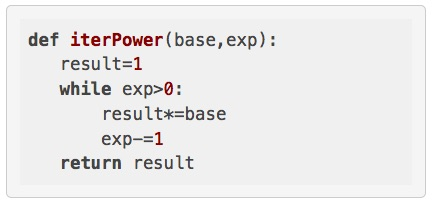
\includegraphics[width=0.5\linewidth]{Body/figures/overcode/largest_stack_cropped.jpg}
\caption{\DIFaddFL{A solution synthesized by OverCode that represents 1538 student solutions.}}
\label{largestStack}
\end{figure}

\section{Solution Variation}

\DIFadd{The taxonomy for }{\it \DIFadd{solution variation}} \DIFadd{used in this thesis has three branches: correctness, approach, }\DIFaddend and \DIFdelbegin \DIFdel{trade-offs, augmented by computation behind the scenes. }\DIFdelend \DIFaddbegin \DIFadd{readability. Since correctness is difficult to prove for an arbitrary piece of code, it is approximated in industry and education by correctness with respect to a set of test cases. In education, the machinery that checks for correctness is often called an autograder.
}\DIFaddend 

\DIFdelbegin \DIFdel{The challenge of scaling up computer science education is usually framed as simply coping with the problems of large class sizes. This thesis, however, explores how the volume of students and their solutions can be exploited to enable new types of rapid personalized feedback, as well as recover aspects of a traditional small class}\DIFdelend \DIFaddbegin \DIFadd{There is a wide range of solutions that pass all the test cases and are labeled correct by the autograder, but they are not all equally good. Figure~\ref{table:diffapproaches} shows three different solutions of widely varying approach and readability that are correct with respect to the autograder test cases.
}

\begin{figure}
\begin{tabular}{ll}
{\bf \DIFaddFL{Iterative Solution}} & {\bf \DIFaddFL{Recursive Solution}} \\
\begin{minipage}{0.5\linewidth}
\begin{lstlisting}[basicstyle=\linespread{1.0}\ttfamily\footnotesize,language=python]
\DIFaddFL{def power(base,exp):
    result=1
    while exp>0:
        result*=base
        exp-=1
    return result
}\end{lstlisting}
\end{minipage}
&
\begin{minipage}{0.5\linewidth}
\begin{lstlisting}[basicstyle=\linespread{1.0}\ttfamily\footnotesize,language=python]
\DIFaddFL{def power(base,exp):
    if exp == 0:
        return 1
    else:
        return base * power(base, exp-1)
}\end{lstlisting}
\end{minipage} \\
%DIF >  \end{tabular}

%DIF >  \begin{tabular}{l}
{\bf \DIFaddFL{Poorly Written Solution}} & \\
\begin{minipage}{0.5\linewidth}
\begin{lstlisting}[basicstyle=\linespread{1.0}\ttfamily\footnotesize,language=python]
\DIFaddFL{def power(base, exp):
    tempBase=base
    result = base
}

    \DIFaddFL{if type(base)==int:
        while exp==0:
            result = 1
            print(result)
            break
        exp=exp-1
        while exp >0:
            tempCal=abs(tempBase)
            exp=exp-1
            while exp<0:
                break
            for i in range (1,tempCal):
                result=result+base
                tempCal=tempCal-1
                tempRes=base
            base=result
        return(result)
}

    \DIFaddFL{else:
        result = 1
        while exp > 0:
            result = result* base
            exp = exp- 1
        return result
}\end{lstlisting}
\end{minipage} 
\end{tabular}
\caption{\DIFaddFL{Three different solutions that exponentiate a base to an exponent. They are all marked correct by the autograder because they pass all the autograder test cases.}}
\label{table:diffapproaches}
\end{figure}

\DIFadd{Solutions can have different approaches. For example, a student might be subversive and disregard a request by the teacher to solve the problem without using an existing equivalent library function. Or the student might include unnecessary lines of code that reveal possible misconceptions about how the language works. Figure~\ref{table:morediffapproaches} gives an example of each.
}

\begin{figure}
\begin{tabular}{ll}
{\bf \DIFaddFL{Subversive Solution}} &  \\
\begin{minipage}{0.5\linewidth}
\begin{lstlisting}[basicstyle=\linespread{1.0}\ttfamily\footnotesize,language=python]
\DIFaddFL{def power(base, exp):
  return base**exp
}\end{lstlisting}
\end{minipage}
& \\
%DIF >  \end{tabular}

%DIF >  \begin{tabular}{l}
{\bf \DIFaddFL{Solution with Unnecessary Statement}} & \\
\begin{minipage}{1.0\linewidth}
\begin{lstlisting}[basicstyle=\linespread{1.0}\ttfamily\footnotesize,language=python]
\DIFaddFL{def power(base,exp):
 result=1
 while exp>0:
     result=result*base
     exp-=1
     continue #keyword here does not change execution
 return result
}\end{lstlisting}
\end{minipage} 
\end{tabular}
\caption{\DIFaddFL{Two different approaches to solving the problem. The first disregards teacher instructions to not use equivalent library functions and the second includes the keyword }\texttt{\DIFaddFL{continue}} \DIFaddFL{in a place where it is completely unnecessary, casting doubt on student understanding of the keyword }\texttt{\DIFaddFL{while}}\DIFaddFL{.}}
\label{table:morediffapproaches}
\end{figure}

\DIFadd{Approaches can be common or uncommon. One can think of the students submitting solutions as a generative function that produces a distribution of solutions we could characterize and take into account while teaching or designing new course material. Figure~\ref{table:commonuncommon} shows the most common and one of the most uncommon solutions produced by students for a problem assigned in 6.00x, an introductory programming course offered on edX in the fall of 2012. Uncommon solutions may be highly innovative or extraordinarily poor.
}

\begin{figure}
\begin{tabular}{ll}
{\bf \DIFaddFL{Common Solution}} & {\bf \DIFaddFL{Uncommon solution}} \\
\begin{minipage}{0.5\linewidth}
\begin{lstlisting}[basicstyle=\linespread{1.0}\ttfamily\footnotesize,language=python]
\DIFaddFL{def power(base,exp):
  result=1
  while exp>0:
      result*=base
      exp-=1
  return result
}\end{lstlisting}
\end{minipage}
& 
%DIF >  \end{tabular}

%DIF >  \begin{tabular}{l}
 %DIF >  & \\
\begin{minipage}{1.0\linewidth}
\begin{lstlisting}[basicstyle=\linespread{1.0}\ttfamily\footnotesize,language=python]
\DIFaddFL{def power(base,exp):
  if exp == 0:
      return 1
  else:
      return base * power(base, exp-1)
}\end{lstlisting}
\end{minipage} 
\end{tabular}
\caption{\DIFaddFL{Common and uncommon solutions to exponentiating a base to an exponent produced by students in the 6.00x introductory Python programming course offered by edX in the Fall of 2012.}}
\label{table:commonuncommon}
\end{figure}

\DIFadd{Readability is the third critical component of solution variation. Poorly written solutions like the one in Figure~\ref{table:diffapproaches} may be both the symptom and the cause of student confusion. Unreadable code is harder to understand and debug, for both teacher and student. In industry, peer-to-peer code reviews help prevent code with poor readability from entering code bases, where it can be difficult and costly to maintain.
}

{\it \DIFadd{Student design choices}} \DIFadd{affect correctness, approach, and readability. Examples include choosing }\texttt{\DIFadd{for}} \DIFadd{over ~}\texttt{\DIFadd{while}}\DIFadd{, }\texttt{\DIFadd{a *= b}} \DIFadd{over }\texttt{\DIFadd{a = a*b}}\DIFadd{, and recursive over iteration. Solution variation is a result of these choices. Even simple differences, like comments, statement order, formatting and variable names can make solutions look quite different to the unaided eye, as shown in Figure~\ref{table:difflook}}\DIFaddend .

\DIFdelbegin \DIFdel{Learners individually solving programming or digital hardware design problems can collectively generate a wide variety of possible bugs and solutions.
  A single programming or digital hardware design exercise may yield thousands of student solutions that vary in many ways, some superficial and some fundamental. For teachers, this variation can, for example, be a source of pedagogically valuable examples and corner cases that slipped past an automatic grader. For students, the variation in a large class means that other students may have struggled along a similar solution path, hit the same bugs, and can offer hints based on that earned expertise. 
}\DIFdelend \DIFaddbegin \begin{figure}
\begin{tabular}{ll}
%DIF >  {\bf Solution } & {\bf Uncommon solution} \\
\begin{minipage}{0.5\linewidth}
\begin{lstlisting}[basicstyle=\linespread{1.0}\ttfamily\footnotesize,language=python]
\DIFaddFL{def iterPower(base, exp):
  '''
  base: int or float.
  exp: int >= 0
}\DIFaddendFL 

  \DIFdelbeginFL \DIFdelFL{Understanding large-scale variation in student solutions requires identifying appropriate features of solutions, developing ways to automatically extract those features from each solution, user interface design to communicate the results to teachers or students, and possibly the collection of additional information from students through learnersourcing. This thesis includes the development of four systems that take advantage of the solution variation in large classes. All four systems have been evaluated using data or live deployments in on-campus or edX courses with hundreds or thousands of students}\DIFdelendFL \DIFaddbeginFL \DIFaddFL{returns: int or float, base^exp
  '''
  result = 1
  while exp > 0:
      result *= base
      exp -= 1
  return result
}\end{lstlisting}
\end{minipage}
& 
%DIF >  \end{tabular}

%DIF >  \begin{tabular}{l}
 %DIF >  & \\
\begin{minipage}{1.0\linewidth}
\begin{lstlisting}[basicstyle=\linespread{1.0}\ttfamily\footnotesize,language=python]
\DIFaddFL{def iterPower(base, exp):
  wynik = 1
}

  \DIFaddFL{while exp > 0:
      exp -= 1  #exp argument is counter
}

      \DIFaddFL{wynik *= base
}

  \DIFaddFL{return wynik
}\end{lstlisting}
\end{minipage} 
\end{tabular}
\caption{\DIFaddFL{These two solutions only differ by comments, statement order, formatting, and variable names. Note: }\texttt{\DIFaddFL{wynik}} \DIFaddFL{means `result' in Polish.}}
\label{table:difflook}
\end{figure}

\section{A Challenge and an Opportunity}

\DIFadd{When teachers may have hundreds or thousands of raw student solutions to the same problem, it becomes arduous or impractical to review them by hand. And yet, only testing for approximate correctness via test cases has been automated. Identifying student solution approaches and readability automatically are still open areas of research. Given the volume and variety of student solutions, how do teachers comprehend what their students wrote? How do they give feedback on approach and readability at scale? 
}

\DIFadd{What value can }{\it \DIFadd{only}} \DIFadd{be extracted from a massive programming class? This thesis focuses on the opportunity posed by exploiting solution variation within large datasets of student solutions to the same problem. With algorithms, visualizations and interfaces, teachers may learn from their students by exposing student solutions they did not know about before. Teachers could find better examples to pull out for discussion. Teachers could write better feedback, test cases, and evaluation rubrics, given new knowledge of the distribution of student solutions across the dimensions of correctness, approach, and readability. And students could be tapped as experts on the solutions they create and the bugs they fix}\DIFaddend .

\section{A Tale of Two Turing Machines}

\DIFdelbegin \DIFdel{This work began after midnight in the basement computer lab of the Stata Center, where a student was struggling to create a Turing Machine that could detect whether a string of open and closed parentheses was properly balanced. If he was not successful within the next day or two, he would fail Computer Architecture (6.004). I will refer to him as Paul. I had a hard time helping Paul turn his Turing machine into one that would pass all the automatic grader's test tapes. I }\DIFdelend \DIFaddbegin \DIFadd{A short story about my time as a teaching assistant illustrates some of the challenges posed by solution variation. Students were programming simulated Turing machines, which compute by reading and writing to a simulated infinitely long tape. I struggled to help a student whose approach was not familiar to me. I }\DIFaddend could not tell if \DIFdelbegin \DIFdel{his approach could work with a little debugging or }\DIFdelend \DIFaddbegin \DIFadd{the approach }\DIFaddend was fatally flawed \DIFaddbegin \DIFadd{or unusual and possibly innovative}\DIFaddend . I did not want to \DIFdelbegin \DIFdel{demoralize him by telling him to abandon his efforts so far and start over unless it was truly necessary. And what if he was on the path to a novel solution no one else had created before?
}\DIFdelend \DIFaddbegin \DIFadd{dissuade him from a novel idea simply because I did not recognize it.
}\DIFaddend 

\DIFdelbegin \DIFdel{While not a necessary condition for the correctness of his intended approach, finding a similar working solution in the pool of previous student submissions would serve as an existence proof and evidence that he should persevere.
I had copies of hundreds of other students' correct Turing machines, but it was difficult to see by inspection whether any of these solutions were successful implementations of his intended approach. This was due to both superficial static and dynamic differences between solutions. There are two sources of static superficial differences: (1) students design their own symbol library and state names for the finite state machine portion of their Turing machine (2) students can list behavioral specifications in terms of their custom symbol and state names in any arbitrary order. Each behavior-specifying rule is a computer-readable version of the form ``if you're in state X and you read symbol Y on the tape, overwrite symbol Y with symbol Z, move the tape-reader in direction W, and transition to state Q." Dynamic superficial differences arise because even after translating these textual statements into a finite state machine diagram, the diagrams look very different from one correct solution to the next.
}%DIFDELCMD < 

%DIFDELCMD < %%%
\DIFdel{Eventually, through trial and error, he got his Turing Machine to work on all the test tapes, and passed the course. But I was deeply troubled by the experience. I felt like the information was there, in our staff server, but my brain could not see through the superficial textual differences nor mentally execute all the studentsolutions I had access to in order to have the perspective that would have helped me help Paul, when I could not see the bugs in his Turing Machine directly. }%DIFDELCMD < 

%DIFDELCMD < %%%
\DIFdel{After the semester ended, I looked into this further. I ran all the correct two-state Turing machines collected during the semester on the same test tape containing a string of open and closed parentheses. The movement of the tape-reading head across this input was logged in coordinates relative to the common starting point, at the left end of the test tape, and displayed along the vertical axis. The horizontal axis represents the number of steps taken by the Turing machine on its way to completing the task. These discrete steps are analogous to time. 
}%DIFDELCMD < 

%DIFDELCMD < %%%
\DIFdel{The majority (88\% ) of the solutions employ one of two mutually exclusive strategies. These strategies were identified just from visual inspection of the movement of many Turing machines across the common test tape. Figure \ref{turingFig} shows their locations on the common input tape over time, separated by strategy into Figures \ref{tapeMoveA} and \ref{tapeMoveB}. These two strategies for determining whether or not the tape's string of parentheses is balanced are (1) matching the innermost open parenthesis with the innermost closed parenthesis, i. e., standard semantic interpretation in math, and (2) matching the $n^{th}$ }%DIFDELCMD < \todo{fix this font} %%%
\DIFdel{open parenthesis with the $n^{th}$ closed parenthesis. The remaining 12}\DIFdelend \DIFaddbegin \DIFadd{The staff server had thousands of previously submitted correct student solutions, but I could not easily see if one of them successfully employed the same approach as the one envisioned by the struggling student. After experimenting with different representations, I found a visualization of Turing machine behavior on test cases that separated 90\% of the correct student solutions into two main approaches~\mbox{%DIFAUXCMD
\cite{ICERGlassman}}%DIFAUXCMD
. The remaining approximately 10}\DIFaddend \% of solutions \DIFdelbegin \DIFdel{(not shown) include }\DIFdelend \DIFaddbegin \DIFadd{included }\DIFaddend less common strategies. \DIFdelbegin \DIFdel{This analysis also exposes room for improvement in the suite of test tapes: at least two strategies in this group are known to pass the test tapes but are actually incorrect because they cannot handle an arbitrary depth of nested parentheses. }%DIFDELCMD < 

%DIFDELCMD < %%%
%DIF < Each staff member is encouraged to complete the Turing Machine lab on their own before counseling students. 
\DIFdel{Staff members were aware of the Turing machine solution they each had found on their own time, and yet were }\DIFdelend \DIFaddbegin \DIFadd{Two solutions passed all test cases but subverted teacher instructions. Many teaching staff members were }\DIFaddend not aware that there were \DIFdelbegin \DIFdel{two mutually exclusive common solutions }\DIFdelend \DIFaddbegin \DIFadd{multiple solutions to the problem and that the current test suite was insufficient to distinguish correct solutions from incorrect ones}\DIFaddend . At least one staff member admitted steering students away from solutions they did not recognize, but in retrospect may have indeed been valid solutions.

\DIFdelbegin \DIFdel{Based on my analysis, I was able to brief fellow 6.004 staff members on the space of solutions--both good and bad--in preparation for subsequent semesters and could suggest additions to the test tape suite to catch submissions that were previously erroneously marked as correct. 
}\DIFdelend \DIFaddbegin \section{Research Questions}
\DIFaddend 

\DIFdelbegin \DIFdel{This experience was a critical and formative one for me. It has inspired the design approach and technical approach taken in many of the systems that follow.
}\DIFdelend \DIFaddbegin \DIFadd{When a teacher cannot read all the student solutions to a programming problem because there are too many of them,
} \begin{itemize} 
\item {\bf \DIFadd{R1}} \DIFadd{how can the teacher understand the common and uncommon variation in their student solutions?
}\item {\bf \DIFadd{R2}} \DIFadd{how can the teacher give feedback on approach and readability at scale?
}\item {\bf \DIFadd{R3}} \DIFadd{... in a personalized way?
}\item {\bf \DIFadd{R4}} \DIFadd{... and how can students do the same?
} \end{itemize} 
\DIFadd{In this thesis, several systems and workflows are developed and studied to better answer these questions. 
}\DIFaddend 

\DIFdelbegin %DIFDELCMD < \begin{figure*}[p]
%DIFDELCMD < 

%DIFDELCMD < \begin{subfigure}[b]{1.0\textwidth}
%DIFDELCMD < \centering
%DIFDELCMD < 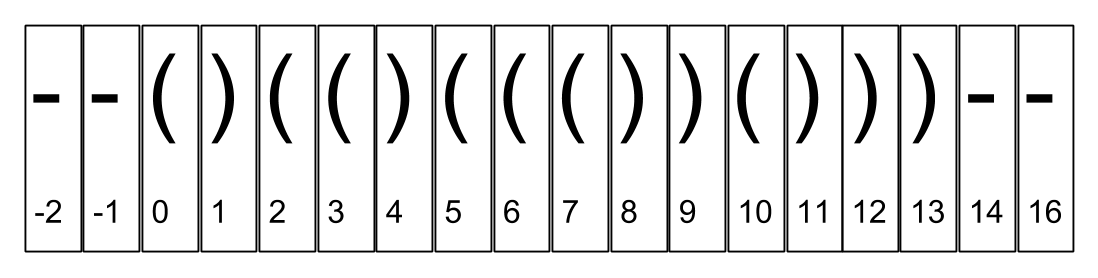
\includegraphics[width=140mm]{Body/figures/ICERtapeLocations.png}
%DIFDELCMD < %%%
%DIFDELCMD < \caption{%
{%DIFAUXCMD
\DIFdelFL{Tape on which all 148 two-state Turing machines were tested, and the numbering system by which locations along the test tape are identified.}}
%DIFAUXCMD
%DIFDELCMD < %DIFDELCMD < \label{tapeLocations}%%%
%DIFDELCMD < \end{subfigure}
%DIFDELCMD < 

%DIFDELCMD < \begin{subfigure}[b]{1.0\textwidth}
%DIFDELCMD < \centering
%DIFDELCMD < 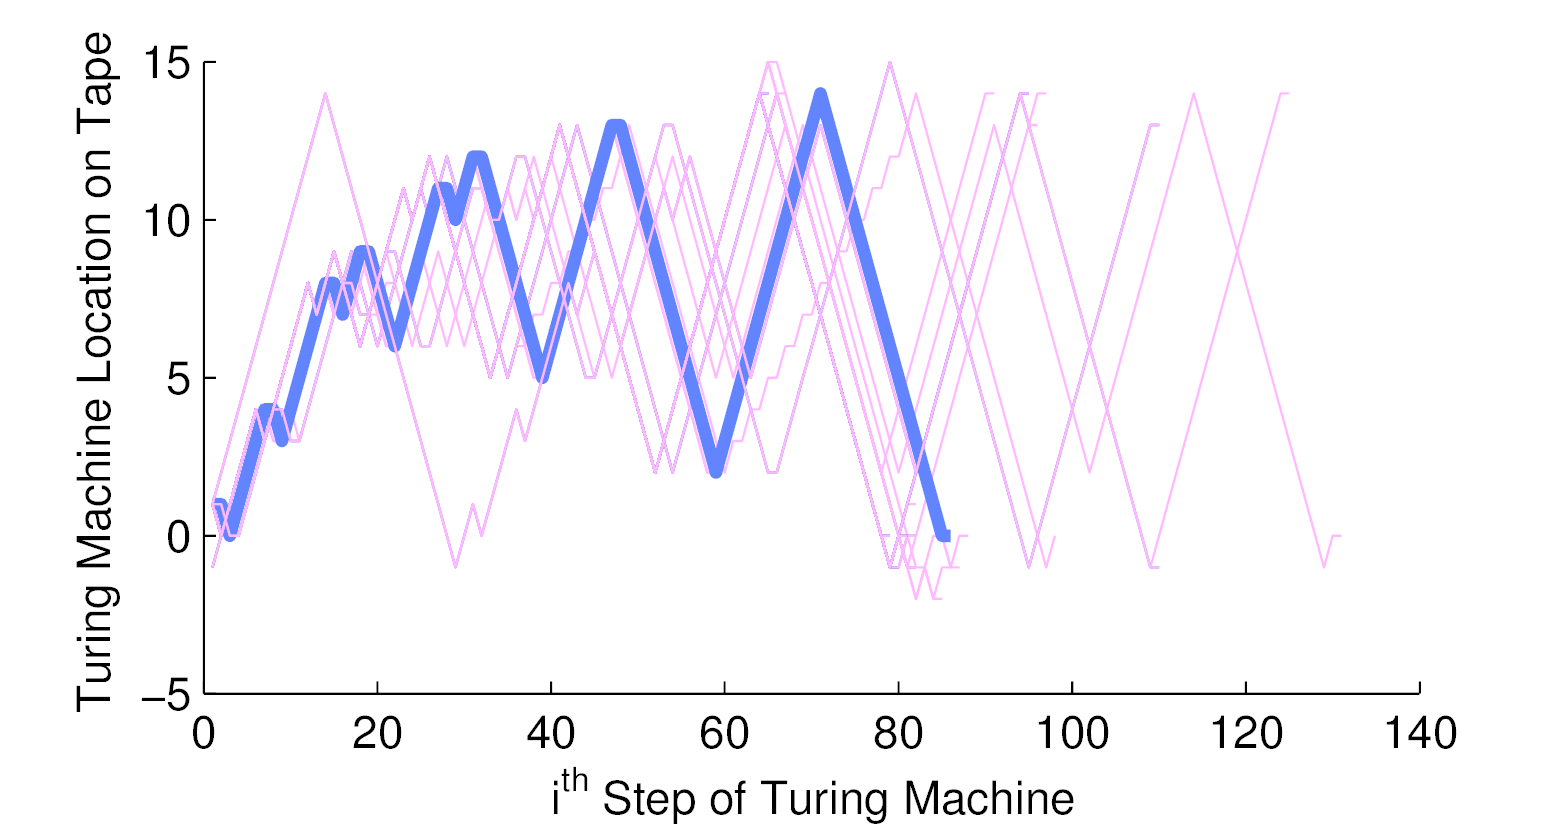
\includegraphics[width=0.85\textwidth]{Body/figures/tmvisualization_InnerParensMatched_allkidsAnno2}
%DIFDELCMD < %%%
%DIFDELCMD < \caption{%
{%DIFAUXCMD
\DIFdelFL{Strategy A Turing machines: those which paired inner sets of open and closed parentheses, as is standard in mathematical notation. (73 out of 148 Turing machines)}}
%DIFAUXCMD
%DIFDELCMD < %DIFDELCMD < \label{tapeMoveA}%%%
%DIFDELCMD < \end{subfigure}
%DIFDELCMD < 

%DIFDELCMD < \begin{subfigure}[b]{1.0\textwidth}
%DIFDELCMD < \centering
%DIFDELCMD < 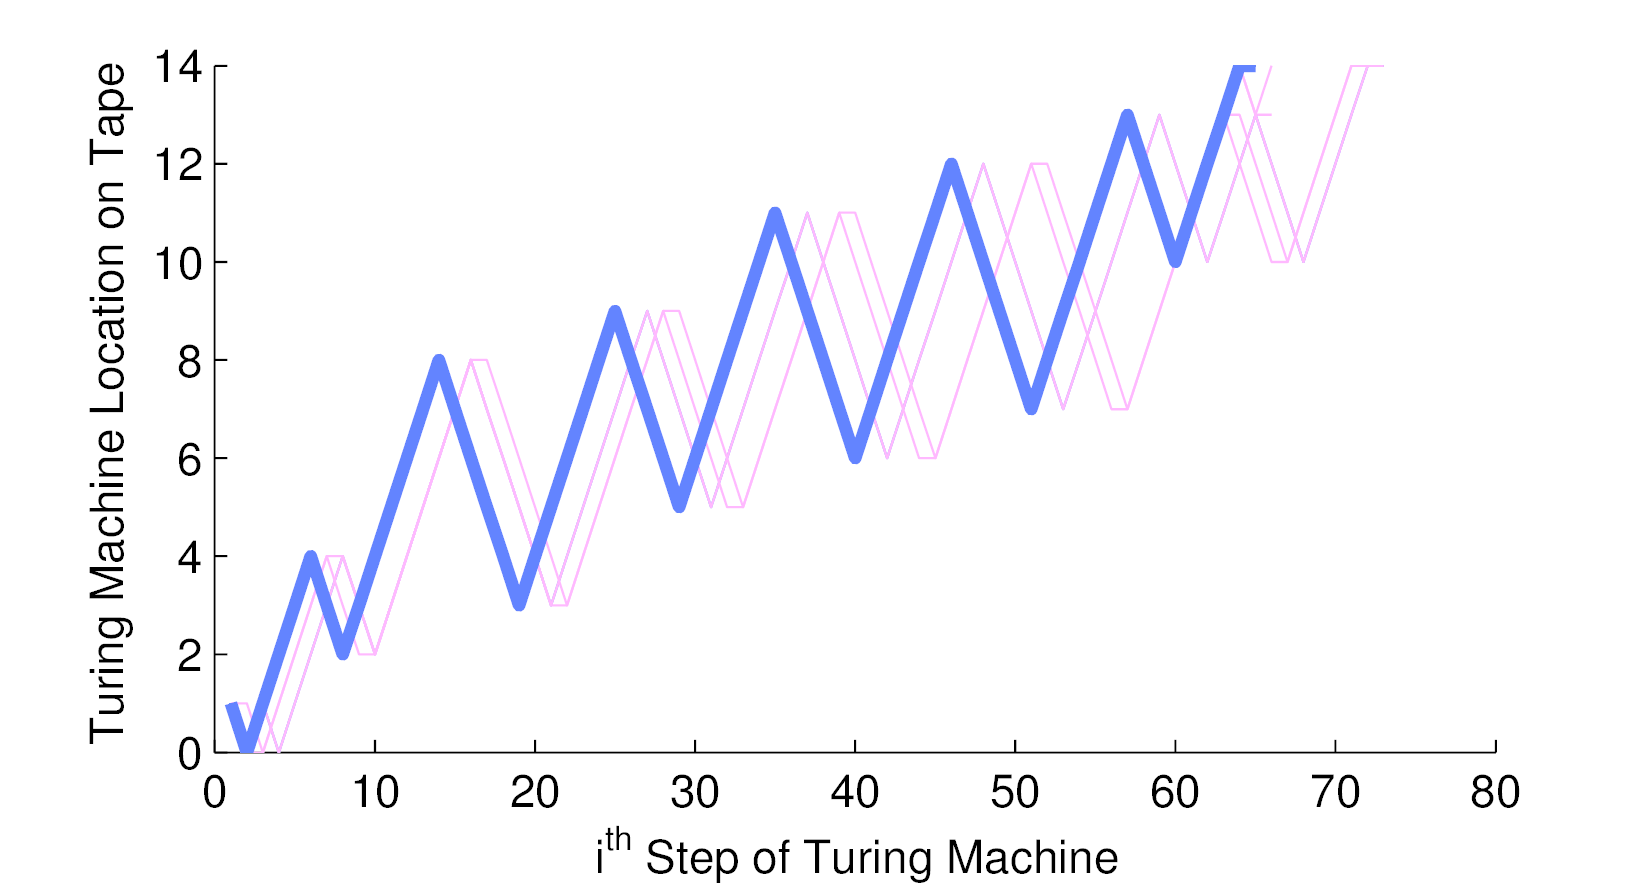
\includegraphics[width=0.85\textwidth]{Body/figures/tmvisualization_NtoNParensMatched_allkidsAnno2}
%DIFDELCMD < %%%
%DIFDELCMD < \caption{%
{%DIFAUXCMD
\DIFdelFL{Strategy B Turing machines: those which paired the first open with the first closed parenthesis, the second open with the second closed parenthesis, etc. (58 out of 148 Turing machines)}}
%DIFAUXCMD
%DIFDELCMD < %DIFDELCMD < \label{tapeMoveB}%%%
%DIFDELCMD < \end{subfigure}
%DIFDELCMD < 

%DIFDELCMD < %%%
%DIF <  \begin{subfigure}[b]{1.0\textwidth}
%DIF <  \includegraphics[scale=0.85]{Body/figures/tmvisualization_Other_allkidsAnno}
%DIF <  \caption{The trajectories of the 17 remaining Turing machines, run on the same common test tape as above, which have yet to be categorized. Both bold trajectories correspond to solutions that do not work in general, but passed the provided, fixed test suite.}
%DIF <  \label{tapeMoveC}
%DIF <  \end{subfigure}
%DIFDELCMD < 

%DIFDELCMD < %%%
%DIFDELCMD < \caption{%
{%DIFAUXCMD
\DIFdelFL{The two most common strategies for a two-state Turing machine to determine if a string of parentheses is balanced. Figures \ref{tapeMoveA} and \ref{tapeMoveB} show tape head position over time on the tape illustrated in Fig. \ref{tapeLocations}. The bold trajectories represent particularly clean examples.}}
%DIFAUXCMD
%DIFDELCMD < %DIFDELCMD < \label{turingFig}%%%
%DIFDELCMD < \end{figure*}
%DIFDELCMD < 

%DIFDELCMD < \section{OverCode}
%DIFDELCMD < 

%DIFDELCMD < %%%
\DIFdel{In MOOCs, a single programming exercise may produce thousands of solutions from learners. Understanding solution variation is important for providing appropriate feedback to students at scale. The wide variation among these solutions can be a source of pedagogically valuable examples, and can be used to refine the autograder for the exercise by exposing corner cases. We developed OverCode to visualize and explore thousands of small Python programs that solve the same problem. 
}\DIFdelend \DIFaddbegin \DIFadd{The OverCode and Foobaz systems both give teachers a better understanding of student solutions and how they vary in approach and readability. }\DIFaddend OverCode \DIFdelbegin \DIFdel{uses both static and dynamic analysis to cluster similar solutions , and lets teachers further filter and cluster solutions based on different criteria. We evaluated OverCode against a non-clustering baseline in a within-subjects study with 24 teaching assistants, and found that the OverCode interface }\DIFdelend allows teachers to more quickly develop a high-level view of student understanding and misconceptions\DIFdelbegin \DIFdel{, and to provide feedback that is }\DIFdelend \DIFaddbegin \DIFadd{. Foobaz displays the variety of common and uncommon variable names in student solutions to a single programming problem, so teachers can better understand student naming practices. The clustering and visualization techniques created for both these systems provide some new answers to the research question }{\bf \DIFadd{R1}} \DIFadd{for introductory Python problems. 
}

\DIFadd{OverCode also helps answer research question }{\bf \DIFadd{R2}}\DIFadd{. With OverCode, teachers produced feedback on solution approaches that was }\DIFaddend relevant to more student solutions\DIFaddbegin \DIFadd{, compared to feedback informed by status quo tools}\DIFaddend . 

\DIFdelbegin %DIFDELCMD < \begin{figure}
%DIFDELCMD < \centering
%DIFDELCMD < 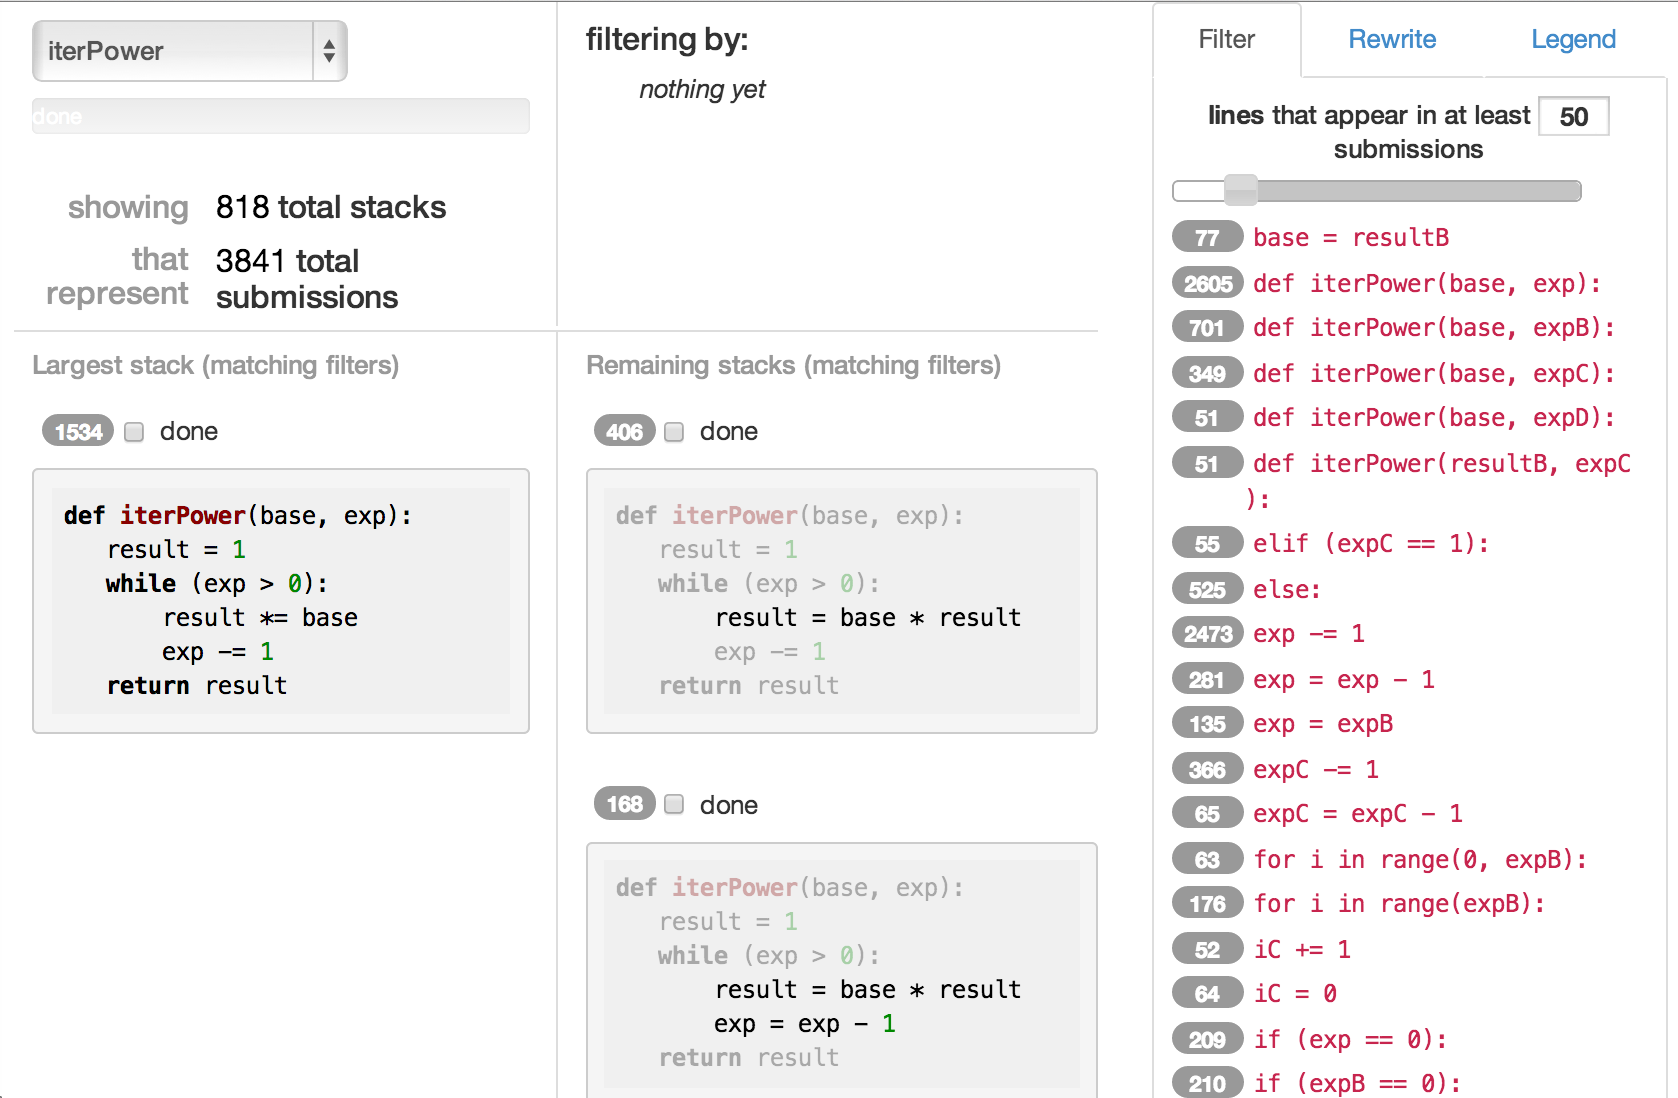
\includegraphics[width=1.0\linewidth]{Body/figures/interfaceScreenShot.png}
%DIFDELCMD < %%%
%DIFDELCMD < \caption{%
{%DIFAUXCMD
\DIFdelFL{The OverCode user interface. The top left panel shows the number of clusters, called }%DIFDELCMD < {\it %%%
\DIFdelFL{stacks}%DIFDELCMD < }%%%
\DIFdelFL{, and the total number of solutions visualized. The next panel down in the first column shows the largest stack, while the second column shows the remaining stacks. The third column shows the lines of code occurring in the cleaned solutions of the stacks together with their frequencies.}}
%DIFAUXCMD
%DIFDELCMD < %DIFDELCMD < \label{fullinterface}%%%
%DIFDELCMD < \end{figure}
%DIFDELCMD < 

%DIFDELCMD < \section{Foobaz}
%DIFDELCMD < 

%DIFDELCMD < %%%
\DIFdel{Traditional feedback methods, such as hand-grading student code for substance and style, are labor intensive and do not scale. We created a new user interface that addresses feedback at scale for a particular and important aspect of code quality}\DIFdelend \DIFaddbegin \DIFadd{The research question }{\bf \DIFadd{R3}} \DIFadd{asks how we can personalize feedback for individual students because personalization, in the form of one-on-one tutoring, has been a gold standard in educational psychology for decades~\mbox{%DIFAUXCMD
\cite{bloom}}%DIFAUXCMD
. For Foobaz, the challenge of delivering personalized feedback on approach and readability at scale was narrowed down to just one critical aspect of readability}\DIFaddend : variable names\DIFdelbegin \DIFdel{(see Figure \ref{fig:figure2}). Foobaz distinguishes variables by their behavior in the program, allowing teachers to comment not only on poor names, but also on names that mislead the reader about the variable 's role. We ran two lab studies of Foobaz, one with teachers and the other with students. In the first study, 10 Python teachers used Foobaz to comment on variable names in thousands of student solutions from an introductory programming MOOC. In the second study, 6 students composed fresh solutions to the same programming problems, and immediately received personalized variable-name quizzes composed in the previous user study. }%DIFDELCMD < 

%DIFDELCMD < \begin{figure}
%DIFDELCMD < 	\centering
%DIFDELCMD < 	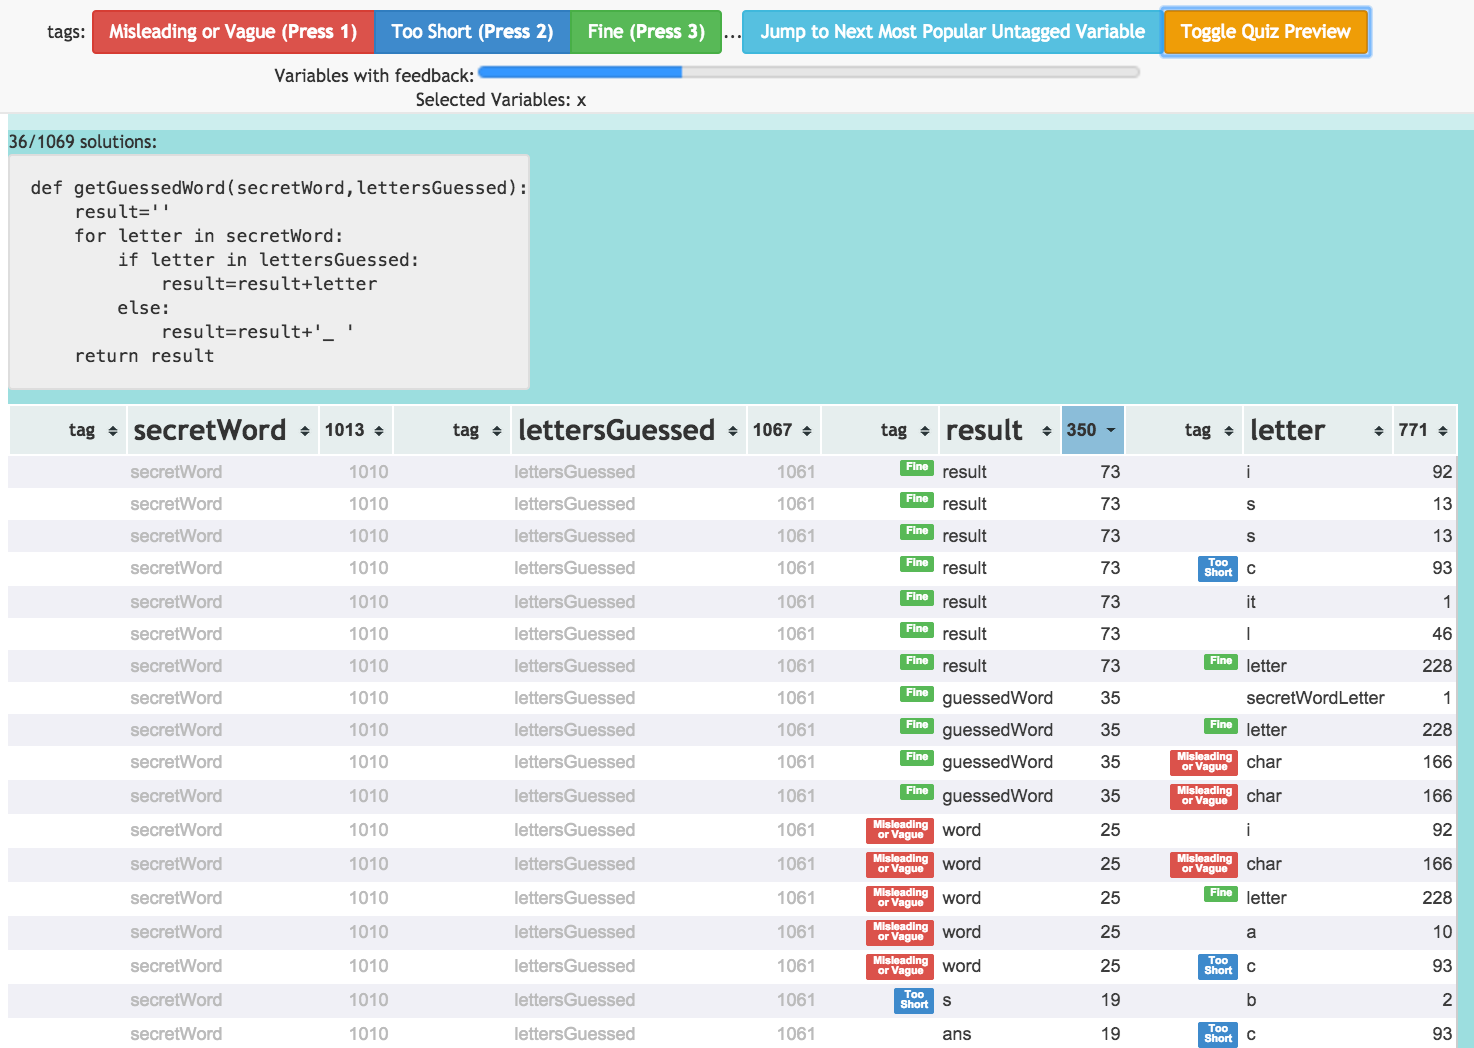
\includegraphics[width=1.0\linewidth]{Body/figures/FoobazInitialFat.png}
%DIFDELCMD < 	%%%
%DIFDELCMD < \caption{%
{%DIFAUXCMD
\DIFdelFL{The Foobaz teacher interface. The teacher is presented with a scrollable list of normalized solutions, each followed by a table of student-chosen variable names. Some names shown here have been labeled by the teacher as ``misleading or vague,'' ``too short,'' or ``fine.''}}
	%DIFAUXCMD
%DIFDELCMD < %DIFDELCMD < \label{fig:figure2}%%%
%DIFDELCMD < \end{figure}
%DIFDELCMD < 

%DIFDELCMD < \todo{include the student view}
%DIFDELCMD < 

%DIFDELCMD < \section{Extensions of OverCode Clustering}
%DIFDELCMD < 

%DIFDELCMD < %%%
\DIFdel{In order to perform more comprehensive clustering, several extensions of the original OverCode clustering methods have been explored and some have been fully implemented. GroverCode is an extension of OverCode built to canonicalize and cluster both correct and incorrect solutions. This was also done in the context of hundreds of exam-level solutions instead of thousands of solutions to "finger exercises" and problem set problems. This change in regime was inspired by need-finding interviews with the lecturer who teaches both the online and residential versions of MIT's introductory Python programming class. She was appreciative of the insights OverCode could give her extracted from the thousands of correct solutions submitted by her online students, but the semi-regular pain of hand-grading the hundreds of incorrect solutions submitted by tuition-paying residential students was a more immediate concern. Adapting to the needs of a team of graders grading a smaller number of more complex solutions, many of which were incorrect, required significant changes to the pipeline and interface. The resulting system was deployed to the staff for use during two grading sessions. The results of this field deployment are also promising; the staff welcomes its continued use in future semesters. More preliminary explorations of statistical methods for clustering solutions are also described.
}%DIFDELCMD < 

%DIFDELCMD < \section{ClassOverflow}
%DIFDELCMD < 

%DIFDELCMD < %%%
\DIFdel{Personalized support for students is a gold standard in education, but it scales poorly with the number of students. Prior work on }\textit{\DIFdel{learnersourcing}} %DIFAUXCMD
\DIFdel{presented an approach for learners to engage in human computation tasks while trying to learn a new skill.Our key insight is that students, through their own experience struggling with a particular problem, can become experts on the particular optimizations they implement or bugs they resolve. The students can then generate hints for fellow students based on their new expertise }\DIFdelend . \DIFdelbegin \DIFdel{ClassOverflow  uses new workflows }\DIFdelend \DIFaddbegin \DIFadd{In a one-on-one scenario, a teacher helping a student might notice that the student is choosing poor variable names. The teacher might start a conversation about both their good and bad variable naming choices. In a massive classroom where that kind of chat is not possible, Foobaz delivers personalized active learning exercises intended to spark the same thought processes in the student. These exercises are called }{\it \DIFadd{variable name quizzes}}\DIFadd{. Foobaz helps answer }{\bf \DIFadd{R3}} \DIFadd{by demonstrating how teachers can compose automatically personalized feedback on an aspect of readability to students at scale.
}

\DIFadd{The final research question, }{\bf \DIFadd{R4}}\DIFadd{, is addressed by two novel workflows that collect and deliver personalized hints. It can be hard to get personalized help in large classes, especially when there are many varied solutions and bugs. Students who struggle, then succeed, become experts on writing particular solutions and fixing particular bugs. The two workflows are built on that insight. Unlike prior incarnations of assigning tasks }\DIFaddend to \DIFdelbegin \DIFdel{harvest and organize students' collective knowledge and advice for helping fellow novices through design problems in engineering (see Figure \ref{fig:workflow}). ClassOverflow was evaluated in an undergraduate digital hardware design class with hundreds of students. We show that, given our design choices, students can create helpful hints for their peers that augment or even replace teachers' personalized assistance, especially when that assistance is not available}\DIFdelend \DIFaddbegin \DIFadd{and collecting data from learners, i.e., learnersourcing~\mbox{%DIFAUXCMD
\cite{kim2013learnersourcing}}%DIFAUXCMD
, these workflows collect and distribute hints written only by students who earned the expertise necessary to write them. Both workflows give students an opportunity to reflect on their own technical successes and mistakes, which is helpful for learning~\mbox{%DIFAUXCMD
\cite{dewey1933} }%DIFAUXCMD
and currently lacking in the engineering education status quo~\mbox{%DIFAUXCMD
\cite{asee}}%DIFAUXCMD
. One of the two workflows also systematically exposes students to some of the variation present in other student solutions, as recommended by theories from educational psychology, specifically variation theory~\mbox{%DIFAUXCMD
\cite{marton1997learning} }%DIFAUXCMD
and analogical learning theory~\mbox{%DIFAUXCMD
\cite{kurtz01learning,loewenstein2003analogical}}%DIFAUXCMD
}\DIFaddend .

\DIFdelbegin %DIFDELCMD < \begin{figure}
%DIFDELCMD < \centering
%DIFDELCMD < 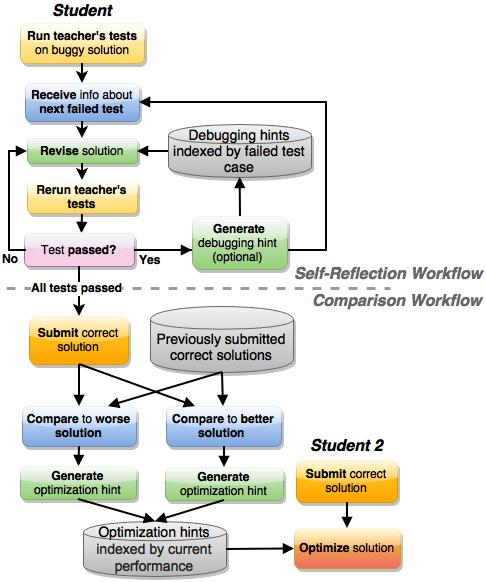
\includegraphics[width=1.0\linewidth]{Body/figures/classoverflow/CombinedWorkflow_CameraReady_FIXED_2.jpg}
%DIFDELCMD < %%%
%DIFDELCMD < \caption{%
{%DIFAUXCMD
\DIFdelFL{In the }\textit{\DIFdelFL{self-reflection}} %DIFAUXCMD
\DIFdelFL{workflow, students generate hints by reflecting on an obstacle they themselves have recently overcome. In the }\textit{\DIFdelFL{comparison}} %DIFAUXCMD
\DIFdelFL{workflow, students compare their own solutions to those of other students, generating a hint as a byproduct of explaining how one might get from one solution to the other.}}
%DIFAUXCMD
%DIFDELCMD < %DIFDELCMD < \label{fig:workflow}%%%
%DIFDELCMD < \end{figure}
%DIFDELCMD < %%%
\DIFdelend \DIFaddbegin \section{Thesis Statement and Contributions}
\DIFaddend 

\DIFdelbegin %DIFDELCMD < \begin{comment}
%DIFDELCMD < \section{Discussion}
%DIFDELCMD < %%%
\DIFdel{Learnersourcing has been a recurring topic at CSCW recently, and these systems }\DIFdelend \DIFaddbegin \DIFadd{The systems described in this thesis }\DIFaddend show various mechanisms for \DIFdelbegin \DIFdel{leveraging learners in large engineering classes. Learners }\DIFdelend \DIFaddbegin \DIFadd{handling and taking advantage of solution variation in massive programming courses. Students }\DIFaddend produce many variations of solutions to a problem, running into common and uncommon bugs along the way. \DIFdelbegin \DIFdel{Learners can be part of a closed system workflow that prompts them to generate analysis of their own activity and sends it to selected fellow learners as feedback. Alternatively, learners can be }\DIFdelend \DIFaddbegin \DIFadd{Students can be }\DIFaddend pure producers whose \DIFdelbegin \DIFdel{activity is analyzed by systems and distilled by teachersinto personalized feedback for fellow learners. We would like to demo these systems together, as a suite of learnersourcing systems that allow teachers to turn the challenges of teaching at scale into an opportunity for discussion, self-reflection, peer-teaching, and more learning from examples. }%DIFDELCMD < \end{comment}
%DIFDELCMD < %%%
\DIFdelend \DIFaddbegin \DIFadd{solutions are analyzed and displayed to teachers. Alternatively, students can be prompted to generate analysis of their own and others' solutions, for the benefit of themselves and current and future students. %DIF > , and sends it to selected fellow learners as feedback. %We would like to demo these systems together, as a suite of learnersourcing systems that allow teachers to turn the challenges of teaching at scale into an opportunity for discussion, self-reflection, peer-teaching, and more learning from examples.
}\DIFaddend 

\DIFdelbegin %DIFDELCMD < \todo{block-quote this}
%DIFDELCMD < {\bf %%%
\DIFdelend My thesis statement is: 
\DIFaddbegin \begin{displayquote}
\DIFaddend Clustering and visualizing solution variation collected from programming courses can help teachers gain insights into student design choices, detect autograder failures, award partial credit, use targeted learnersourcing \DIFdelbegin %DIFDELCMD < \todo{make sure targeted learnersourcing is defined} %%%
\DIFdelend to collect hints for other students, and give personalized style feedback at scale.
\DIFdelbegin %DIFDELCMD < }
%DIFDELCMD < %%%
\DIFdelend \DIFaddbegin \end{displayquote}
\DIFaddend 

\DIFdelbegin %DIFDELCMD < \section{Terminology}
%DIFDELCMD < 

%DIFDELCMD < \todo{Finish defining: solutions, programming exercise/problem, collections of solutions to an exercise....}
%DIFDELCMD < 

%DIFDELCMD < %%%
\DIFdel{Since terminology across research domains can vary, I will define the terms in which I will describe previous research and my own}\DIFdelend \DIFaddbegin \DIFadd{The main contributions of this thesis are}\DIFaddend :
 \begin{itemize} 
\item \DIFdelbegin \DIFdel{A }%DIFDELCMD < {\it %%%
\DIFdel{solution}%DIFDELCMD < } %%%
\DIFdel{is code that a particular person wrote in response to a prompt or problem description.
}\DIFdelend \DIFaddbegin \DIFadd{An algorithm that uses the behavior of variables to help cluster Python solutions and generate the platonic solution for each cluster. Platonic solutions are readable and encode both static and dynamic information, i.e., the syntax carries the static information and the variable name encodes dynamic information.
}\DIFaddend \item \DIFdelbegin %DIFDELCMD < {\it %%%
\DIFdel{Solution clusters}%DIFDELCMD < } %%%
\DIFdel{represent different patterns of implementation. For example, there may be two distinct solution clusters, both achieving the same input-output behavior but by different means. }%DIFDELCMD < \todo{better name for this, that respects topic model approach?}
%DIFDELCMD < \item %%%
\item%DIFAUXCMD
\DIFdelend A \DIFdelbegin %DIFDELCMD < {\it %%%
\DIFdel{solution path}%DIFDELCMD < } %%%
\DIFdel{is a series of code snapshots generated while a person is working toward meeting a particular input-output behavior specification. 
}%DIFDELCMD < \item %%%
\item%DIFAUXCMD
\DIFdel{The }%DIFDELCMD < {\it %%%
\DIFdel{space of student solutions}%DIFDELCMD < } %%%
\DIFdel{refers to the aggregation of student-generated solutions and the solution clusters they form. }%DIFDELCMD < \item {\it %%%
\DIFdel{Learnersourcing}%DIFDELCMD < }%%%
\DIFdel{... }%DIFDELCMD < \todo{define, using my own wording if necessary}
%DIFDELCMD < \end{itemize}
%DIFDELCMD < 

%DIFDELCMD < \section{Contributions}
%DIFDELCMD < 

%DIFDELCMD < \todo{add grovercode contributions, turn into prose}%%%
\DIFdel{The main contributions of this thesis are:
}%DIFDELCMD < \begin{itemize}
%DIFDELCMD < \item %%%
\item%DIFAUXCMD
\DIFdel{A }\DIFdelend novel visualization that \DIFdelbegin \DIFdel{shows }\DIFdelend \DIFaddbegin \DIFadd{highlights }\DIFaddend similarity and variation among thousands of Python solutions \DIFdelbegin \DIFdel{, with cleaned code shown }\DIFdelend \DIFaddbegin \DIFadd{while displaying platonic solutions }\DIFaddend for each variant. 
\item \DIFdelbegin \DIFdel{An algorithm that uses the behavior of variables to help cluster Python solutions and generate the cleaned code for each cluster of solutions.
}%DIFDELCMD < \item %%%
\item%DIFAUXCMD
\DIFdelend Two user studies that show this visualization is useful for giving teachers a \DIFdelbegin \DIFdel{birds-eye }\DIFdelend \DIFaddbegin \DIFadd{bird's-eye }\DIFaddend view of thousands of students' Python solutions.
\item A \DIFaddbegin \DIFadd{grading interface that shows similarity and variation among Python solutions, with faceted browsing so teachers can filter solutions by error signature, i.e., the test cases they pass and fail. 
}\item \DIFadd{Two field deployments of the grading interface within introductory Python programming exam grading sessions.
}\item \DIFadd{A }\DIFaddend technique for displaying clusters of Python solutions with only \DIFdelbegin \DIFdel{a slice }\DIFdelend \DIFaddbegin \DIFadd{an aspect, i.e., variable names and roles, }\DIFaddend of each cluster exposed, revealing the \DIFdelbegin \DIFdel{features }\DIFdelend \DIFaddbegin \DIFadd{details }\DIFaddend that are relevant to the task. \DIFdelbegin \DIFdel{In this application, the relevant features are variable names and roles.
}\DIFdelend %DIF > In this application, the relevant features are variable names and roles.
\item A workflow for generating personalized active learning exercises, emulating how a teacher might socratically discuss good and bad choices with a student while they review the student's solution together. 
\item \DIFdelbegin \DIFdel{A working system which implements }\DIFdelend \DIFaddbegin \DIFadd{An implementation of }\DIFaddend the above technique and method for \DIFdelbegin \DIFdel{datasets from both MOOCs and large residential classes on introductory Python programming. }\DIFdelend \DIFaddbegin \DIFadd{variable naming. %DIF >  within datasets from both MOOCs and large residential classes on introductory Python programming.
}\DIFaddend \item Two lab studies which evaluate both the \DIFdelbegin \DIFdel{teachers' and students' }\DIFdelend \DIFaddbegin \DIFadd{teacher and student }\DIFaddend experience of the \DIFdelbegin \DIFdel{variable name feedback workflow .
}%DIFDELCMD < \item{A self-reflection learnersourcing workflow in which students generate hints for each other by reflecting on an obstacle they themselves have recently overcome while debugging their solution to a Python or digital design exercise.}
%DIFDELCMD < \item{A comparison learnersourcing workflow in which students generate design hints for each other by comparing their own solutions to alternative designs submitted by other students.} 
%DIFDELCMD < \item{A deployment of the self-reflection workflow in a 200-student class and a lab study of the comparison workflow with 9 participants. Results from these studies show that personalized hints can be viably learnersourced, and that these hints serve as helpful guides to fellow students encountering the same obstacle or attempting to reach the same goal.}
%DIFDELCMD < %%%
\DIFdelend \DIFaddbegin \DIFadd{workflow applied to variable names.
}\item \DIFadd{A self-reflection learnersourcing workflow in which students generate hints for each other by reflecting on an obstacle they themselves have recently overcome while debugging their solution.
}\item \DIFadd{A comparison learnersourcing workflow in which students generate design hints for each other by comparing their own solutions to alternative designs submitted by other students.
}\item \DIFadd{Deployments of both workflows in a 200-student digital circuit programming class, and an in-depth lab study with 9 participants.
}\DIFaddend  \end{itemize} 

\section{Thesis Overview}

Chapter \ref{chapter:relatedwork} summarizes prior and contemporary relevant research on systems that support programming education. It also briefly explains theories from the learning sciences and psychology literature that influenced or support the pedagogical value of the design choices made within this thesis.

The four chapters that follow describe, in detail, the four systems developed, as well as their evaluation on archived data or in the field.

 \begin{itemize} 
\item OverCode (Chapter \ref{chapter:overcode}) visualizes thousands of programming solutions using static and dynamic analysis to cluster similar solutions. It lets teachers quickly develop a high-level view of student understanding and misconceptions and provide feedback that is relevant to many student solutions. \DIFaddbegin \DIFadd{It also describes GroverCode, an extension of OverCode optimized for grading correct and incorrect student solutions.
}\DIFaddend 

\item Foobaz (Chapter \ref{chapter:foobaz}) clusters variables in student \DIFdelbegin \DIFdel{programs }\DIFdelend \DIFaddbegin \DIFadd{solutions }\DIFaddend by their names and behavior so that teachers can give feedback on variable naming. Rather than requiring the teacher to comment on thousands of students individually, Foobaz generates personalized quizzes that help students evaluate their own names by comparing them with good and bad names from other students. 

\item \DIFdelbegin \DIFdel{ClassOverflow (Chapter \ref{chapter:classoverflow} ) collects and organizes }\DIFdelend \DIFaddbegin \DIFadd{Chapter \ref{chapter:classoverflow} describes two workflows that collect and organize }\DIFaddend solution hints indexed by \DIFaddbegin \DIFadd{(1) }\DIFaddend the autograder test that failed or \DIFaddbegin \DIFadd{(2) }\DIFaddend a performance characteristic like size or speed. It helps students reflect on their debugging or optimization process, generates hints that can help other students with the same problem, and could potentially bootstrap an intelligent tutor tailored to the problem.

\item \DIFdelbegin \DIFdel{OverCode Extensions (Chapter \ref{chapter:grovercode} ) describes (1) GroverCode, an extension to OverCode optimized for processing and displaying incorrect as well as correct student submissions and (2) }\DIFdelend \DIFaddbegin \DIFadd{Chapter \ref{chapter:grovercode} describes Bayesian }\DIFaddend clustering and mixture modeling algorithms applied to the OverCode pipeline \DIFdelbegin \DIFdel{'s output for }\DIFdelend \DIFaddbegin \DIFadd{output for extracting }\DIFaddend additional insight into patterns within student solutions. 
%DIF < The GroverCode user interface is optimized and deployed in the field for teachers awarding partial credit to each of the hundreds of students who submitted programs in computer-based quizzes and final exams for the residential Python-based introductory programming (6.0001) and data science (6.0002) courses at MIT.
 \end{itemize} 

Chapter \ref{chapter:discussion} discusses \DIFdelbegin \DIFdel{the design lessons that apply to the entire collection of }\DIFdelend \DIFaddbegin \DIFadd{some of the insights that came out of building and testing the }\DIFaddend systems in this thesis. Chapter \DIFdelbegin \DIFdel{\ref{chapter:futurework} }\DIFdelend \DIFaddbegin \DIFadd{\ref{chapter:conclusion} }\DIFaddend outlines avenues of future work \DIFdelbegin \DIFdel{this thesis work}\DIFdelend \DIFaddbegin \DIFadd{on the systems and ideas in this thesis}\DIFaddend , in combination with the complementary work of others in this space\DIFdelbegin \DIFdel{, paves the way for.
}%DIFDELCMD < 

%DIFDELCMD < \begin{comment}%%%
\DIFdel{"one-on-one tutoring promotes both greater student learning and increased student motivation to learn compared with traditional, formal classroom teaching and learning settings" --http://www.ncbi.nlm.nih.gov/pmc/articles/PMC3292071/ }%DIFDELCMD < \end{comment}
%DIFDELCMD < 

%DIFDELCMD < \begin{comment}
%DIFDELCMD < 

%DIFDELCMD < %%%
\DIFdel{Dead kittens:
}%DIFDELCMD < 

%DIFDELCMD < %%%
\DIFdel{In introductory programming and digital circuit design education, this thesis aims to change the traditional curve in the quality of education as a function of class size from monotonically decreasing to a U-shape. As a proxy for measuring learning outcomes, the systems developed in this thesis empower old or entirely new rapid, personalized feedback modes similar to those delivered in a one-on-one teaching relationship but enabled by the scale of students composing solutions to class exercises.
}%DIFDELCMD < 

%DIFDELCMD < %%%
\DIFdel{By second grade, children should be able to write simple, coherent stories \mbox{%DIFAUXCMD
\cite{http://www.webmd.com/parenting/features/when-should-kids-learn-read-write-math}}%DIFAUXCMD
. 
}%DIFDELCMD < 

%DIFDELCMD < %%%
\DIFdel{When I was much younger, my dad taught me about vacuum tubes. With few modifications, tubes can serve as amplifiers, switches, or displays. ``Tube: The Invention of Television'' tells the dramatic history behind the invention and commericialization of the first televisions, which were built with cathode ray tubes. At critical parts of the story, he'd ask, e.g., ``How you would change the intensity of the electron beam hitting the screen?'' just before the authors were about to reveal how the inventors would get past their next technological hurdle.
}%DIFDELCMD < 

%DIFDELCMD < %%%
\DIFdel{Sometimes, I had no idea how to answer. Sometimes, I came up with something similar to what the inventors came up with. And sometimes, because I was not biased by the actual scientific literature that the inventors were immersed in, I came up with something very different, but possibly also effective. 
}%DIFDELCMD < 

%DIFDELCMD < %%%
\DIFdel{The systems in this thesis help teachers take advantage of the massive collections of solutions, enabling either (1) the same teaching practices that were previously only tractable in smaller courses or (2) new practices that are only possible when a massive collection of student solutions are available.
}%DIFDELCMD < 

%DIFDELCMD < %%%
\DIFdel{This thesis describes several systems designed to (1)  (2) (3) amplify teachers' actions, by enabling them to compose and deliver personalized feedback to more students while expending minimal additional effort. 
}%DIFDELCMD < 

%DIFDELCMD < %%%
\DIFdel{Despite recent advances in artificial intelligence, human and computer intelligence remain largely complementary. Humans can compose new questions and handle novel answers, while computers can perform prescribed analyses of thousands of student answers orders of magnitude faster than humans. 
}%DIFDELCMD < 

%DIFDELCMD < %%%
\DIFdel{Ways of delivering the rapid, personalized feedback that  commonly accepted practices of good teaching d
}%DIFDELCMD < 

%DIFDELCMD < %%%
\DIFdel{As enrollment in programming courses grows, some teaching practices and systems may become prohibitively expensive or arduous to use.
}%DIFDELCMD < 

%DIFDELCMD < %%%
\DIFdel{This thesis documents several novel tools I developed for helping hundreds or thousands of students learn how to program. The demand for programming education is growing rapidly, and this thesis treats the volume of students in programming classes not as a problem, but as an opportunity. It begins with the story of how I learned to program, and ends with a description of new tools for teachers and students engaged in the hard work of transferring the knowledge and practice of programming from one generation to the next.
}%DIFDELCMD < 

%DIFDELCMD < %%%
\DIFdel{At heart, I'm an electrical engineer, and it has informed my approach through-out. To me, a class of students is a system I want closed-loop control over: with the control policy of an experienced teacher and knowledge of the state of the system--my hundreds or thousands of students--I can better steer it to my intended destination of knowledge and skills.
}%DIFDELCMD < 

%DIFDELCMD < %%%
\DIFdel{I similarly think of solutions as systems that turn inputs into outputs, sometimes in the same way, sometimes in different ways.
}%DIFDELCMD < \end{comment}
%DIFDELCMD < 

%DIFDELCMD < %%%
\DIFdelend \DIFaddbegin \DIFadd{.
}\DIFaddend \chapter{Related Work}\label{chapter:relatedwork}

Systems that help students in massive programming courses may build on work from \DIFdelbegin \DIFdel{any or all the following related fields: }\DIFdelend program analysis, program synthesis, crowd workflows, \DIFdelbegin \DIFdel{user-interface }\DIFdelend \DIFaddbegin \DIFadd{user interface }\DIFaddend design, machine learning, intelligent tutoring systems, natural language processing, data mining, and learning science. \DIFdelbegin \DIFdel{First, I present prior work and theories of how people learn that later inspired key design decisions. I then clarify how this thesis work is novel while describing related work that achieves similar goals or uses similar methods. %DIF < \todo{add references to my own work, to illustrate relevance}
}\DIFdelend \DIFaddbegin \DIFadd{This chapter summarizes relevant technical and psychological work that supports the pedagogical value of the systems developed in this thesis and gives context to the technical contributions. %DIF > \todo{rewrite chapter description} %First, I present prior work and theories of how people learn that later inspired key design decisions or suggest that the systems in this thesis are beneficial in a learning environment. I then clarify how this thesis work is novel while describing related work that achieves similar goals or uses similar methods. %\todo{add references to my own work, to illustrate relevance}
}\DIFaddend 

\DIFdelbegin %DIFDELCMD < \section{Scalable teaching principles}
%DIFDELCMD < %%%
\DIFdelend %DIF > \todo{rewrite this paragraph}

%DIF < Learning how to write programs, or at least how to “think computationally,” has gained national attention in the last year. Last September, New York City Mayor Bill de Blasio announced that all public schools in NYC will be required to offer computer science to all students by 2025. In January, the White House released its “Computer Science For All” initiative, “offering every student the hands-on computer science and math classes that make them job-ready on day one” (President Obama, 2016 State of the Union Address).
\DIFaddbegin \section{Clustering}
\DIFaddend 

%DIF < Schools like MIT, Stanford, Berkeley and the University of Washington have expanded to accommodate hundreds or thousands of students in a single programming class. Many more complete exercises on tutorial websites like Codecademy, Kahn Academy, and Code School or enroll in coding schools and bootcamps like General Assembly and Hackbright Academy. One-on-one tutoring is considered a gold standard in education, and the teacher-to-student ratio is only getting worse.
%DIF > \todo{add citations}

%DIF < As we develop new tools, techniques, and curriculum to serve more students, it is important to be grounded in, or at least knowledgeable of, the work that researchers in educational psychology have been doing for decades: teasing apart what it takes to learn something efficiently and well.
\DIFdelbegin %DIFDELCMD < 

%DIFDELCMD < %%%
\DIFdel{There are many factors inside and outside the classroom that have significant effects on learning.I will focus on a few techniques and theories from the learning sciences that a human may be able to execute better with a computer than without. Therefore, peer groups, home environment, learning communities, and identity formation~\mbox{%DIFAUXCMD
\cite{walberg1984improving,case2008education} }%DIFAUXCMD
are beyond our consideration}\DIFdelend \DIFaddbegin \DIFadd{Grouping similar items, i.e., }{\it \DIFadd{clustering}}\DIFadd{, is a fundamental human activity for organizing, making sense of, and drawing conclusions from data. Across many scientific fields, clustering goes by different names but serves a common purpose: helping humans explore, interpret, and summarize data~\mbox{%DIFAUXCMD
\cite{Jain50}}%DIFAUXCMD
}\DIFaddend .

%DIF < There is an entire literature on developing sustainable communities of practice that foster student development and mastery, much the way a traditional judo dojo operates. There is also great work on how identity formation can help budding experts persist and thrive in a learning environment. For a high level treatment of both those literatures as they pertain to engineering education, read this brief handbook for practitioners: Education theories on learning: an informal guide for the engineering education scholar.
\DIFdelbegin %DIFDELCMD < 

%DIFDELCMD < %%%
%DIF < However, I will focus on a few theories and concepts that specifically help teachers develop more effective presentations of information and exercises for practice. This short-list of ideas, techniques, and benchmarks from educational psychology have guided my own development of tools for teachers teaching hundreds or thousands of programming students at once.
%DIFDELCMD < 

%DIFDELCMD < \subsection{Tutoring}
%DIFDELCMD < 

%DIFDELCMD < %%%
\DIFdel{Tutoring has been held up as a gold standard in education since 1984 when Bloom published a collection of his lab's work demonstrating tutoring's efficacy relative to other experimental and conventional methods at the time~\mbox{%DIFAUXCMD
\cite{bloom}}%DIFAUXCMD
. }\DIFdelend \DIFaddbegin \DIFadd{This is }{\it \DIFadd{unsupervised machine learning}}\DIFadd{. There are no labels, no ground truth. }\DIFaddend For example, \DIFdelbegin \DIFdel{his lab found that, after 11 sessions of instruction in probability or cartography, elementary and middle school students who received tutoring in groups of one to three were, on average, two standard deviations better than their counterparts in a conventional 30-person classroom. Given the expense of scaling up one-on-one tutoring, Bloom challenged the academic community to find a method of group instruction that was just as good, or better. That challenge still stands as a benchmark that modern systems and techniques can compare against. While I do not measure the relative learning gains associated with the systems presented in this thesis, I do relate key design decisions to the tutoring best practices that are able to be scaled up or automated, such as prompting for self-explanations}\DIFdelend \DIFaddbegin \DIFadd{is there one true clustering of all the articles the New York Times ever published? Humans have goals, and how useful clusters are to them is all that matters}\DIFaddend .
%DIF <  evidence from the learning sciences The focus on this thesis is on developing systems that scale up what good tutors and teachers do.

\DIFdelbegin %DIFDELCMD < \subsubsection{Reflection and Self-Explanation}
%DIFDELCMD < %%%
\DIFdelend \DIFaddbegin \DIFadd{Humans are pattern finders. A human can look at collections of items and group them in various ways. For example, a collection of dogs could be grouped according to their size or the color of their fur. Both clusterings are equally valid. Clustering by size may be more useful if the purpose is to decide which dogs get walked together.
}\DIFaddend 

\DIFdelbegin \DIFdel{Effective tutors often have characteristics described by Lepper and Wolverton's INSPIRE model: superior domain and pedagogical content knowledge, nurturing relationships with students, progressive content delivery, Socratic styles that prompt students to explain and generalize, and feedback on solutions, not students~\mbox{%DIFAUXCMD
\cite{wood2012role}}%DIFAUXCMD
. Turns et al. \mbox{%DIFAUXCMD
\cite{asee} }%DIFAUXCMD
argue that the absence of reflection in traditional engineering education is a significant shortcoming. This thesis contributes systems designed to address that shortcoming}\DIFdelend \DIFaddbegin \DIFadd{Computers need more instructions before they can step in and help cluster items, when there are too many for a human to cluster them alone. Items need to be represented in a machine-readable way, and human judgements need to be replaced with computation}\DIFaddend .

\DIFdelbegin \DIFdel{Self-explanations are generated by the student for themselves; they are a form of reflection, which is a critical method for triggering the transformation from conflict and doubt into clarity and coherence \mbox{%DIFAUXCMD
\cite{dewey1933}}%DIFAUXCMD
. Students self-explanations foster the integration of new knowledge, while some tutors' explanations may be insufficient or flawed, due to }\DIFdelend \DIFaddbegin \DIFadd{The first critical decision when preparing a collection for clustering by a computer is how to represent the items in a machine-readable format, e.g., as images or sets of attributes, also called }{\it \DIFadd{features}}\DIFadd{, like weight, height, and fur color. This }{\it \DIFadd{representation}} \DIFadd{effects every subsequent step of the clustering process~\mbox{%DIFAUXCMD
\cite{Jain50}}%DIFAUXCMD
. Since the clustering is performed for a human with a goal, the representation ideally captures aspects of }\DIFaddend the \DIFdelbegin \DIFdel{curse of knowledge~\mbox{%DIFAUXCMD
\cite{birch2007curse}}%DIFAUXCMD
. Effective tutors encourage self-explanation by prompting students with questions like "Why?" and "How?"~\mbox{%DIFAUXCMD
\cite{selfexplanation}}%DIFAUXCMD
. Students of tutors who fostered self-explanations had learning gains similar to those whose tutors provided their own explanations and feedback\mbox{%DIFAUXCMD
\cite{chi2001learning}}%DIFAUXCMD
. }\DIFdelend \DIFaddbegin \DIFadd{items that are relevant to that goal.
}\DIFaddend 

%DIF < One insight stands out: the value of self-explanation for fostering student learning.
\DIFaddbegin \DIFadd{Further customizing the item representation for the human goal, also known as }{\it \DIFadd{feature extraction}}\DIFadd{, is optional but often very helpful. Feature extraction is computing new features about each item from the original representation. These new features may better capture the aspects of items that are relevant to the human goal. For example, if the goal is to partition dogs by fur color and dogs are represented by images, one might extract the most common color in every dog image.
}\DIFaddend 

%DIF < \subsubsection{Self-Explanation}
\DIFaddbegin \DIFadd{A second optional step is }{\it \DIFadd{feature selection}}\DIFadd{, the process of determining what features can be ignored because they are irrelevant to the human goal. For example, if the goal is to partition dogs by fur color and dogs are represented by collections of features, then only the fur color feature may be selected, ignoring height and weight.
}\DIFaddend 

%DIF < Reflection is also a critical method for triggering the transformation from conflict and doubt into clarity and coherence \cite{dewey1933}. Turning that reflection into a self-explanation further improves understanding \cite{selfexplanation}.
\DIFdelbegin %DIFDELCMD < 

%DIFDELCMD < \begin{comment}
%DIFDELCMD < %%%
\DIFdel{Turns et al. \mbox{%DIFAUXCMD
\cite{asee} }%DIFAUXCMD
argue that the absence of reflection in traditional engineering education is a significant shortcoming.
}%DIFDELCMD < \end{comment}
%DIFDELCMD < 

%DIFDELCMD < %%%
%DIF < \subsubsection{Curse of Knowledge}
%DIFDELCMD < 

%DIFDELCMD < %%%
%DIF < While explanations generated by tutees may help them integrate new knowledge, explanations generated by experts, i.e., the tutor, may be insufficent or flawed, due to the curse of knowledge \cite{birch2007curse}.
%DIFDELCMD < 

%DIFDELCMD < %%%
%DIF < Reflection is a critical method for triggering the transformation from conflict and doubt into clarity and coherence \cite{dewey1933}. Turning that reflection into a self-explanation further improves understanding \cite{selfexplanation}. According to Turns et al. \cite{asee}, the absence of reflection in traditional engineering education is a significant shortcoming. 
%DIFDELCMD < 

%DIFDELCMD < \subsection{Deliberate Practice}
%DIFDELCMD < 

%DIFDELCMD < %%%
%DIF < Ericsson is one of the foremost experts on how learners can efficiently acquire domain-specific knowledge and skills, like those necessary for becoming an effective programmer. 
%DIFDELCMD < 

%DIFDELCMD < %%%
\DIFdel{Deliberate practice is generally accepted to be goal directed, effortful, not enjoyable, repetitive, accompanied by rapid feedback, and only sustained as long as the learner can be fully concentrated on the task, i.e., no more than a few hours~\mbox{%DIFAUXCMD
\cite{Gobet2012}}%DIFAUXCMD
. For example, rather than just playing pickup basketball games in the neighborhood, an aspiring professional player might design specific drills to work on his/her weaknesses.
Teachers help facilitate deliberate practice, because they can design appropriate exercises and provide feedback until the student can differentiate between good and bad performance and provide that feedback to themselves. }%DIFDELCMD < 

%DIFDELCMD < %%%
\DIFdel{Recent work incorporating deliberate practice in large classrooms has demonstrated great benefits. A recent study of undergraduate physics classrooms found that, with deliberate practice as a base of the instructional design, improvements can approach and exceed Bloom's 2-sigma threshold~\mbox{%DIFAUXCMD
\cite{Deslauriers862}}%DIFAUXCMD
. Another recent study confirms the value of rapid feedback in foundation engineering classrooms \mbox{%DIFAUXCMD
\cite{ieeeRapidFeedback}}%DIFAUXCMD
. This thesis contributes systems designed to provide feedback on some aspects of programming tasks where it was not feasible to do so before, such as Foobaz, which stimulates reflection and provides feedback on one of the most basic forms of program readability: variable names}\DIFdelend \DIFaddbegin \DIFadd{Hopefully, at the end of this process, some items are closer to each other than they are to others, with respect to some aspect of the items the human cares about. If a computer is to verify this, one needs to define exactly what the }{\it \DIFadd{closer}} \DIFadd{means. The computer needs a human to define a }{\it \DIFadd{distance function}} \DIFadd{that quantifies how close or far items are from each other}\DIFaddend .

\DIFdelbegin %DIFDELCMD < \subsection{Zone of Proximal Development and Scaffolding}
%DIFDELCMD < 

%DIFDELCMD < %%%
\DIFdel{The concept of the zone of proximal development (ZPD) was first introduced in the mid 1920's by the Soviet pyschologist Lev Vygotsky. It refers to the gap between what a learner can do without help and what a learner cannot yet do, no matter how much help they are given.It is implied that an object of learning strictly outside the ZPD is either too easy or too hard, and little or no learning will occur. }\DIFdelend \DIFaddbegin \DIFadd{The next step is choosing a }{\it \DIFadd{clustering method}}\DIFadd{, i.e., a general strategy. Clustering is finding clusters of items that are closer to each other than they are to items in other groups. There is no one best method for all clustering problems, but some methods produce clusters that support the human's problem-specific goal better than others.
}\DIFaddend 

\DIFdelbegin \DIFdel{Wood et al.~\mbox{%DIFAUXCMD
\cite{woodscaffolding} }%DIFAUXCMD
introduced a complementary processcalled scaffolding. Scaffolding enables a learner to "solve a problem, carry out a task or achieve a goalwhich would otherwise be beyond his unassisted efforts" because the teacher controls the aspects of }\DIFdelend \DIFaddbegin \DIFadd{Some methods have an }{\it \DIFadd{objective function}} \DIFadd{that quantifies some desirable characteristic of clusters to maximize or some undesirable characteristic of clusters to minimize~\mbox{%DIFAUXCMD
\cite{Jain50}}%DIFAUXCMD
. One objective function sums up how different each item is from its cluster center. Presumably, }\DIFaddend the \DIFdelbegin \DIFdel{task that are initially outside the learner's abilities. Recent work suggests that }\DIFdelend \DIFaddbegin \DIFadd{smaller the differences, }\DIFaddend the \DIFdelbegin \DIFdel{maximum learning gains come from giving students the hardest possible tasks they are able, with the assistance of scaffolding, to complete~\mbox{%DIFAUXCMD
\cite{zpd14}}%DIFAUXCMD
. Formative feedback~\mbox{%DIFAUXCMD
\cite{formative} }%DIFAUXCMD
can be helpfulas part of the scaffolding. It should non-evaluative, supportive, timely, and specific. It usually arrives as a response to a student's action, e. g., a hint, an explanation, or a verification based on the student answer. Based on this research, one of the systems in this thesis, ClassOverflow, identifies where a student solution is on the spectrum of optimality and prompts the student to reflect on the }\DIFdelend \DIFaddbegin \DIFadd{better the clustering. Specific clustering algorithms may define different centers for each cluster, tally up the differences in different ways, and follow different processes to minimize the objective function.
}

\DIFadd{Some methods are more easily characterized by their process than their objective function. For example, hierarchical clustering methods are characterized as either:
}

 \begin{itemize} 
\item \DIFaddend {\it \DIFdelbegin \DIFdel{next most optimal}\DIFdelend \DIFaddbegin \DIFadd{agglomerative}\DIFaddend } \DIFdelbegin \DIFdel{solution.
}\DIFdelend \DIFaddbegin \DIFadd{or bottom-up, by merging individual items into small clusters, then merging small clusters into larger clusters, etc., or
}\item {\it \DIFadd{divisive}} \DIFadd{or top-down, by splitting the entire collection of items into clusters, then splitting those clusters into further clusters, until all clusters only contain one item~\mbox{%DIFAUXCMD
\cite{xu2005survey}}%DIFAUXCMD
.
} \end{itemize} 
\DIFaddend 

\DIFdelbegin %DIFDELCMD < \subsection{The Role of Strategic Variation in Examples}
%DIFDELCMD < %%%
\DIFdelend \DIFaddbegin \DIFadd{The objective functions used in these methods help determine which clusters to merge or split.
}\DIFaddend 

\DIFdelbegin \DIFdel{Studies of tutors and their students help us identify characteristics and styles of interaction that help explain the effectiveness of tutoring. Some of these can be successfully deployed in large classrooms. However, the way we frame content can also have large effects on how students understand, generalize, and transfer their learning to new contexts.
}\DIFdelend \DIFaddbegin \DIFadd{Some statistical clustering methods, such as mixture models, assume that the items are samples from underlying, unseen distributions of items. By making some assumptions about what those distributions might look like, an algorithm can map items to clusters to maximize a statistical measure of fit between the observed data and the unobserved distributions.
}\DIFaddend 

\DIFdelbegin \DIFdel{Concrete examples of an object of learning--like how to apply an appropriate statistical test in a statistics word problem--vary in ways that are superficial, e.g., irrelevant , and fundamental, e. g., relevant. In the language of educational psychologists, these are often called surface and structural features~\mbox{%DIFAUXCMD
\cite{quilicimayer}}%DIFAUXCMD
. A simple compare and contrast exercise when solving equations~\mbox{%DIFAUXCMD
\cite{rittle2007does} }%DIFAUXCMD
or examining case studies in negotiation~\mbox{%DIFAUXCMD
\cite{loewenstein2003analogical} }%DIFAUXCMD
can bring this variation to the fore, and yield learning benefits}\DIFdelend \DIFaddbegin \DIFadd{Many methods require the human to provide additional values and thresholds, such as how similar two items need to be to be grouped together or how many clusters to look for. Some methods incorporate techniques that anticipate outliers and attempt to be robust to them}\DIFaddend .

\DIFdelbegin \DIFdel{Learning in the presence of variation in these features helps learners generalize and transfer their knowledge to new situations, such as better transfer of geometric problem solving skills~\mbox{%DIFAUXCMD
\cite{workedexamplesvariability,Variabilityofpractice}}%DIFAUXCMD
. Several educational models, e.g., Variation Theory and the 4C/ID Model~\mbox{%DIFAUXCMD
\cite{van2002blueprints}}%DIFAUXCMD
, build on the value of variability by suggesting specific ways for how it should be deployed in the classroom. The three primary systems in this thesis, OverCode, Foobaz, and ClassOverflow, are all designed to make the natural variability present in student solutions useful to teachers and students, in accordance with recommendations from the educational theories that follow. }\DIFdelend \DIFaddbegin \DIFadd{The types of clusters produced by clustering algorithms can be partitioned in several ways~\mbox{%DIFAUXCMD
\cite{wiki:clustering}}%DIFAUXCMD
, such as:
}\DIFaddend 

\DIFdelbegin %DIFDELCMD < \subsubsection{Analogical Learning}
%DIFDELCMD < %%%
\DIFdelend \DIFaddbegin  \begin{itemize} 
\item {\it \DIFadd{Hard}} \DIFadd{versus }{\it \DIFadd{soft}}\DIFadd{: If each item is mapped to a single cluster, the method is hard. If items can partially belong in different degrees to multiple clusters, the method is soft.
}\item {\it \DIFadd{Partition}} \DIFadd{vs. }{\it \DIFadd{overlap}} \DIFadd{vs. }{\it \DIFadd{hierarchy}}\DIFadd{: If each item belongs to one and only one cluster, the method is producing strict partitions. If each item belongs to one or more clusters, than the method is producing overlapping clusters. If each item belongs to one cluster and clusters are strictly contained by other clusters, the method is hierarchical.
} \end{itemize} 
\DIFaddend 

\DIFdelbegin \DIFdel{Analogies are central to human cognition; they can help learners understand and transfer knowledge and skills to new situations. Analogical learning is at play both when learners have a base of knowledge that they bring with them to a novel target and when they compare two partially understood situations that can illuminate each other, serving as both a source and recipient of information~\mbox{%DIFAUXCMD
\cite{kurtz01learning,loewenstein2003analogical}}%DIFAUXCMD
.
However, in order to reap the full benefits of analogical learning, learners must engage deeply.Reading two cases, serially, in a session is not enough; learners will not necessarily make the necessary connections unless there are explicit instructions to compare~\mbox{%DIFAUXCMD
\cite{loewenstein2003analogical,catrambone1989overcoming}}%DIFAUXCMD
. Kolodner~\mbox{%DIFAUXCMD
\cite{Kolodner} }%DIFAUXCMD
suggests creating software tools that align examples to facilitate analogical learning. This thesis is }\DIFdelend \DIFaddbegin \DIFadd{Some methods do not produce clusters of items, but rather clusters of components within items. For example}\DIFaddend , \DIFdelbegin \DIFdel{in part, a response this suggestion.
}\DIFdelend \DIFaddbegin \DIFadd{Latent Dirichlet Allocation (LDA)~\mbox{%DIFAUXCMD
\cite{lda} }%DIFAUXCMD
does not cluster entire documents. It produces a hard, strict partition of words into different clusters, typically called }{\it \DIFadd{topics}}\DIFadd{. At the level of documents, however, this can look like a soft clustering: an individual document might be 50\% hospital-related words, 30\% government-related words, and 20\% negotiation-related words.
}\DIFaddend 

\DIFdelbegin \DIFdel{Novices may become confused if asked to compare their solution to a fellow student's solution; this is not necessarily bad for learning outcomes.
Piaget theorized that cognitive disequilibrium, experienced as confusion, could trigger learning due to the creation or restructuring of knowledge schema~\mbox{%DIFAUXCMD
\cite{disequilibrium}}%DIFAUXCMD
. D'Mello et al. maintain that confusion can be productive, as long as it is both appropriately injected and resolved~\mbox{%DIFAUXCMD
\cite{productiveconfusion}}%DIFAUXCMD
. Similarly, reflecting on a peer's conceptual development or alternative solution may bring about cognitive conflict that prompts reevaluation of the student's own beliefs and understanding \mbox{%DIFAUXCMD
\cite{kavanagh}}%DIFAUXCMD
. The ClassOverflow system is designed to stimulate this kind of productive confusion, comparison, and resolution through self-explanation. }%DIFDELCMD < \todo{add Towards Providing Feedback to Students in Absence of Formalized Domain Models by Sebastian Gross, Bassam Mokbel, Barbara Hammer, Niels Pinkwart}
%DIFDELCMD < %%%
\DIFdelend \DIFaddbegin \DIFadd{Clusters are hard to objectively evaluate. It is expensive and time consuming to bring in humans with goals to evaluate how useful the clusters are to them. }{\it \DIFadd{Cluster validation}} \DIFadd{refers to the metrics used to approximate the quality of clusters with little or no human input~\mbox{%DIFAUXCMD
\cite{xu2005survey}}%DIFAUXCMD
. These metrics can be the basis of choosing one method over another, one parameter value over another, or one clustering over another quickly but approximately.
}\DIFaddend 

\DIFdelbegin \DIFdel{Analogical learning can be very difficult. For example, the structural features may be aligned between a base and the new target situation, but large differences in surface features will hurt the learner's ability to see any connection~\mbox{%DIFAUXCMD
\cite{Kurtz}}%DIFAUXCMD
.
This may be explained by how human memory works. For novices, the most reliable form of retrieval is based on surface similarity, not deep analogical similarity; experts can more easily retrieve situations that are structurally similar and therefore more relevant for a new situation at hand~\mbox{%DIFAUXCMD
\cite{Loewenstein}}%DIFAUXCMD
.
}%DIFDELCMD < 

%DIFDELCMD < %%%
\DIFdel{Variation Theory, discussed next, is specifically designed to help students more deeply appreciate structural features, which may help them transfer their learning to new situations instead of feeling lost, confused by superficial differences.
}%DIFDELCMD < 

%DIFDELCMD < \subsubsection{Variation Theory: Preventing Human Overfitting}
%DIFDELCMD < 

%DIFDELCMD < %%%
\DIFdel{This aphorism captures the ideas at the heart of Variation Theory (VT) well: }\DIFdelend \DIFaddbegin \DIFadd{Another way to produce more helpful clusterings is to involve the human in an }\DIFaddend {\it \DIFdelbegin \DIFdel{"He cannot, England know, who knows England only ."}\DIFdelend \DIFaddbegin \DIFadd{interactive}\DIFaddend } \DIFdelbegin \DIFdel{VT is concerned with the way in which students are taught from concrete examples.
It is relatively new and still being investigated for its usefulness in a broad range of disciplines, including mathematics and computer science. 
}\DIFdelend \DIFaddbegin \DIFadd{process. The clustering algorithm produces clusters and gives the human one or more ways to give feedback. Feedback could be in the form of indicating what is good or bad about this clustering. Feedback could be the human reaching in and directly moving an item from one cluster to another. The method reruns, based on this new information, and produces a new clustering for the human to evaluate and give feedback on.
}\DIFaddend 

\DIFdelbegin \DIFdel{VT asserts that human learning can suffer from overfitting for some of the same reasons that machine learning algorithms do. Overfitting is a term I am borrowing from the machine learning community. If a machine learning algorithm "thinks" the key difference between photos of cats and dogs is the color of the sky (which is obviously unrelated to distinguishing between photos of cats and dogs), then a possible explanation is that the algorithm was trained on photos with insufficient or biased variation.
If all the cat photos it ever saw were taken on a cloudy day, and all the dog photos it ever saw were taken on a sunny day, could you blame this naive program for latching on to this obvious differentiator of housepet species? Humans can make the same inferential mistake when not exposed to a sufficient variety of examples of an object of learning. VT catalogues a hierarchy of patterns of variation designed to immunize the learner to this kind of mistake}\DIFdelend \DIFaddbegin \DIFadd{One aspect of clustering that does not fall into the traditional conversation about features, distance functions, and methods is }{\it \DIFadd{interpretability}}\DIFadd{. A clustering may have good quality scores with respect to those cluster validation metrics, but if it is difficult for the human to understand what each cluster contains, they may have trouble using it to achieve their goals}\DIFaddend .

\DIFdelbegin \DIFdel{More abstractly, VT is built on the understanding that learning is not possible without being able to discern what the object of learning is ~\mbox{%DIFAUXCMD
\cite{marton1997learning}}%DIFAUXCMD
. Discernment is not possible without experiencing variation in the object of learning and the world in which its situated~\mbox{%DIFAUXCMD
\cite{marton2004classroom}}%DIFAUXCMD
. This variation is described in terms of aspects and features. An aspect refers to a dimension of variation, and a feature is a value of that dimension of variation~\mbox{%DIFAUXCMD
\cite{ling2012variation}}%DIFAUXCMD
. Some features are irrelevant, while critical features collectively define the object of learning.
}%DIFDELCMD < 

%DIFDELCMD < %%%
\DIFdel{For a more concrete discussion of variation, consider the following examples:
}%DIFDELCMD < \begin{enumerate}
 \begin{enumerate} %DIFAUXCMD
%DIFDELCMD < \item %%%
\item%DIFAUXCMD
\DIFdel{The phrase “a heavy object” might not make sense to the reader unless they have interacted with objects of various weights.
}%DIFDELCMD < \item %%%
\item%DIFAUXCMD
\DIFdel{Consider a child who recently learned how to add numbers, but always starts with the larger number: 2+1=3, 4+2=6, etc. Asking the child to add the numbers in the opposite order, smaller number first, and verify that the result is the same introduces the commutative feature of addition. }%DIFDELCMD < \item %%%
\item%DIFAUXCMD
\DIFdel{No matter how wildly a cup diverges from a prototypical exampleof a tea cup, if it does not have the critical feature of being able to hold something, it is not a cup. }
 \end{enumerate} %DIFAUXCMD
%DIFDELCMD < \end{enumerate}
%DIFDELCMD < 

%DIFDELCMD < %%%
\DIFdel{Marton et al.~\mbox{%DIFAUXCMD
\cite{} }%DIFAUXCMD
identify four patterns of variation: contrast, separation, generalization, and fusion. If a child is learning the concept of “three”, then contrast refers to being introduced to three apples, as well as a pair of apples, or a dozen. Generalization refers to being introduced to different groups of three: three apples, three dogs, three beaches, and three languages.
This clarifies that it is not the apples that give “three” its meaning. Separation refers to a pattern of examples that helps the learner separate a dimension of variation from other dimensions of variation. A child could be introduced to a litter of nearly identical puppies that only differ in coat color, for example.
Fusion is the final pattern of variation, where the learner is exposed to examples that vary along all the dimensions of variation at once, since this is most commonly encountered in the real world. These patterns of variation are intended to reveal which aspects of a concept or phenomenon are superficial and irrelevant and which are innate and critical to its definition. }%DIFDELCMD < 

%DIFDELCMD < %%%
\DIFdel{VT is a framework that has guided teaching materials and been used as an analytic framework in a variety of contexts, including lessons on critical reading~\mbox{%DIFAUXCMD
\cite{noble1998contents}}%DIFAUXCMD
, vocabulary learning~\mbox{%DIFAUXCMD
\cite{doi:10.1108/IJLLS-10-2014-0038}}%DIFAUXCMD
, the color of light~\mbox{%DIFAUXCMD
\cite{Ling2006}}%DIFAUXCMD
, mathematics~\mbox{%DIFAUXCMD
\cite{Pythagoras233}}%DIFAUXCMD
, chemical engineering~\mbox{%DIFAUXCMD
\cite{C2RP20145C}}%DIFAUXCMD
, Laplace transforms~\mbox{%DIFAUXCMD
\cite{carstensen2004laplace}}%DIFAUXCMD
, supply and demand~\mbox{%DIFAUXCMD
\cite{marton2006some} }%DIFAUXCMD
and computing education~\mbox{%DIFAUXCMD
\cite{suhonen2007applications}}%DIFAUXCMD
. It has been the subject of a government-funded three-year longitudinal study in Hong Kong, with promising results~\mbox{%DIFAUXCMD
\cite{lo2005each}}%DIFAUXCMD
}\DIFdelend \DIFaddbegin \DIFadd{There are thousands of published methods that exhibit combinations of these properties and strategies. When comparing methods, it is helpful to break the comparison down by representation, features, distance function, objective function, and algorithm they use as well as the type of clusters they produce. In subsequent sections, this language will be used to help describe the many different code analysis and clustering processes found in related work}\DIFaddend .


\DIFdelbegin \DIFdel{In this thesis, Overcode and Foobaz are explicitly designed to discover and make human-interpretable the variation naturally present in student solutions. All the systems in this thesis demonstrate ways in which extracted variation, in solutions or errors, can be used in massive classes. In the next section, I describe efforts to extract, answer questions about, or otherwise make usable the natural variation in corpuses of webpages, apps, and code that do not all have the same purpose. In the final section, I describe similar efforts specifically for corpuses of student solutions to the same programming exercise.
}\DIFdelend \DIFaddbegin \section{Mining Solution Variation}
\DIFaddend 

%DIF < that teachers can more easily employ variation theory-based techniques. %While we do not yet have data that directly compares the effectiveness of VT-inspired lessons to those delivered by personal tutors, programming teachers can keep Variation Theory in mind when they teach concepts, like recursion.
\DIFdelbegin %DIFDELCMD < 

%DIFDELCMD < \section{Exploring and Mining Variation in the Wild}
%DIFDELCMD < 

%DIFDELCMD < %%%
\DIFdelend One important aspect of both engineering and design is that there are multiple ways to solve the same problem\DIFdelbegin \DIFdel{. There are many means to an end, and the optimality of each solution may be context-dependent. Sub-optimality }\DIFdelend \DIFaddbegin \DIFadd{, each with their own trade-offs. The consequences of these design choices can be significant. Suboptimal solutions, including poorly designed code, }\DIFaddend can have high personal, safety, and economic costs. 
\DIFdelbegin \DIFdel{For example, in the software industry, maintenance dominates the cost of producing software~\mbox{%DIFAUXCMD
\cite{fox2013engineering}}%DIFAUXCMD
. Poorly designed code may be the culprit because it requires significantly more maintenance.
}\DIFdelend 

\DIFdelbegin %DIFDELCMD < \begin{comment}
%DIFDELCMD < %%%
\DIFdel{There’s no silver bullet for becoming a great engineer. However, best practices will probably always include analyzing others’ designs, highlighting their successes and failures, as well as composing one’s own designs and receiving critiques from others.
}%DIFDELCMD < 

%DIFDELCMD < %%%
\DIFdel{This method of training is particularly exciting today, when there is such a diversity of design examples available online. Thousands of apps are available for download from app stores. Kaggle maching learning competition submissions are not public by default, but are sometimes released by authors and collected for the benefit of others. Github and Bitbucket host millions of repositories, many of them public and searchable. }%DIFDELCMD < \end{comment}
%DIFDELCMD < 

%DIFDELCMD < %%%
\DIFdel{If solutionscan be indexed in useful ways, they can be mined to ask basic questions like,
}%DIFDELCMD < \begin{enumerate}
%DIFDELCMD < \item    %%%
\DIFdelend \DIFaddbegin \DIFadd{It may be possible to learn good and bad practices from large collections of previous solutions by looking at common and uncommon choices and making judgements about their successes and trade-offs. In order to understand the space of current solutions, there are many questions one could ask. }\DIFaddend In the face of a common design choice, what do \DIFdelbegin \DIFdel{people }\DIFdelend \DIFaddbegin \DIFadd{designers }\DIFaddend most commonly pick? Has this changed over time? \DIFdelbegin %DIFDELCMD < \item    %%%
\DIFdelend What are popular design alternatives? \DIFdelbegin %DIFDELCMD < \item    %%%
\DIFdelend What are examples of design \DIFdelbegin \DIFdel{fails }\DIFdelend \DIFaddbegin \DIFadd{failures }\DIFaddend that should be learned from and never repeated? \DIFdelbegin %DIFDELCMD < \item    %%%
\DIFdelend What are examples of design innovations that are clearly head-and-shoulders above the rest? \DIFdelbegin %DIFDELCMD < \end{enumerate}
%DIFDELCMD < %%%
\DIFdelend The answers to these questions could fuel \DIFdelbegin \DIFdel{instruction }\DIFdelend \DIFaddbegin \DIFadd{education about designing solutions }\DIFaddend that complies with \DIFdelbegin \DIFdel{Variation Theory's recommendations. With }\DIFdelend \DIFaddbegin \DIFadd{variation theory recommendations. }\DIFaddend OverCode, Foobaz, and \DIFdelbegin \DIFdel{ClassOverflow, I }\DIFdelend \DIFaddbegin \DIFadd{the comparison learnersourcing workflow }\DIFaddend try to answer \DIFdelbegin \DIFdel{the same questions for students tackling the same programming challenge}\DIFdelend \DIFaddbegin \DIFadd{these questions for student solutions written in code}\DIFaddend .

\DIFdelbegin %DIFDELCMD < \subsection{Webpages}
%DIFDELCMD < %%%
\DIFdelend %DIF > The same questions could be applied to student solutions to a programming problem, and OverCode, Foobaz, and the targeted learnersourcing workflows attempt to answer them.
\DIFaddbegin 

\subsection{Code Outside the Classroom}

\subsubsection{Web pages}
\DIFaddend Ritchie et al.~\cite{ritchie2011d} describe a user interface for finding \DIFdelbegin \DIFdel{“relevant and inspiringdesign examples?\DIFdelend \DIFaddbegin \DIFadd{helpful, i.e., relevant or inspiring, design examples }\DIFaddend from a curated database of web pages. \DIFdelbegin \DIFdel{This }\DIFdelend \DIFaddbegin \DIFadd{Their }\DIFaddend work is intended to support designers who like to refer to or adapt previous designs for their own purposes. Traditional search engines only index the content of web pages\DIFdelbegin \DIFdel{; this }\DIFdelend \DIFaddbegin \DIFadd{. Their }\DIFaddend system indexes web \DIFdelbegin \DIFdel{pages?\DIFdelend \DIFaddbegin \DIFadd{pages' }\DIFaddend design style by automatically extracting global stylistic and structural features from each page. Instead of manual browsing, users can search and filter a gallery of design-indexed pages. Users can provide an example design in order to find similar and dissimilar designs, as well as high-level style terms like \DIFdelbegin \DIFdel{“minimal.?\DIFdelend \DIFaddbegin \DIFadd{``minimal.''
}\DIFaddend 

Kumar et al.~\cite{webzeitgeist} defined {\it design mining} as \DIFdelbegin \DIFdel{?\DIFdelend \DIFaddbegin \DIFadd{``}\DIFaddend using knowledge discovery techniques to understand design demographics, automate design curation, and support data-driven design tools.\DIFdelbegin \DIFdel{” This }\DIFdelend \DIFaddbegin \DIFadd{'' Their }\DIFaddend work goes beyond searching and filtering a gallery of hundreds of curated \DIFdelbegin \DIFdel{webpages}\DIFdelend \DIFaddbegin \DIFadd{web pages}\DIFaddend . Their Webzeitgeist design mining platform allows users to query a repository of hundreds of thousands of web pages based on the properties of their Document Object Model (DOM) tree and the look of the rendered page. A \DIFdelbegin \DIFdel{1679-dimensional }\DIFdelend vector of descriptive features \DIFdelbegin \DIFdel{are }\DIFdelend \DIFaddbegin \DIFadd{is }\DIFaddend computed for each DOM node in each page.

Webzeitgeist enables users to ask and answer \DIFdelbegin \DIFdel{some of those originally highlighted questions }\DIFdelend \DIFaddbegin \DIFadd{questions like the following}\DIFaddend , with respect to \DIFdelbegin \DIFdel{this }\DIFdelend \DIFaddbegin \DIFadd{a }\DIFaddend large web page repository\DIFdelbegin \DIFdel{:
}%DIFDELCMD < \begin{enumerate}
%DIFDELCMD < \item    %%%
\DIFdelend \DIFaddbegin \DIFadd{. }\DIFaddend What are all the distinct cursors? \DIFdelbegin %DIFDELCMD < \item    %%%
\DIFdelend What are the most popular colors for text? \DIFdelbegin %DIFDELCMD < \item    %%%
\DIFdelend How many DOM tree nodes does a typical page have? How deep is a typical DOM tree? \DIFdelbegin %DIFDELCMD < \item    %%%
\DIFdelend What is the distribution of aspect ratios for images? \DIFdelbegin %DIFDELCMD < \item    %%%
\DIFdelend What are the spatial distributions for common HTML tags? \DIFdelbegin %DIFDELCMD < \item    %%%
\DIFdelend How do web page designers use the HTML canvas element?
\DIFdelbegin %DIFDELCMD < \end{enumerate}
%DIFDELCMD < %%%
\DIFdelend 

To dig into examples of a particular design choice, users can, for example, query for all pages with very wide images. The result is a set of horizontally scrolling pages. Alternatively, users can query for \DIFdelbegin \DIFdel{webpages }\DIFdelend \DIFaddbegin \DIFadd{web pages }\DIFaddend that have a particular layout, like a large header, a navigational element at the top of the page, and a text node containing greater than some threshold of words, in order to see all the examples of pages that fit those layout specifications. Specific combinations of page features can imply high-level designs as well so, with careful query construction, users can query for high-level ideas. For example, querying for pages with a centered HTML input element \DIFdelbegin \DIFdel{AND }\DIFdelend \DIFaddbegin \DIFadd{and }\DIFaddend low visual complexity retrieves many examples that look like the front pages of search engines.

\DIFdelbegin %DIFDELCMD < \subsection{Android Apps}
%DIFDELCMD < %%%
\DIFdelend \DIFaddbegin \subsubsection{Android Apps}
\DIFaddend 

Shirazi et al.~\cite{Shirazi} and Alharbi and Yeh~\cite{Alharbi} describe automated processes for taking apart and analyzing Android app code as well as empirical analyses of \DIFdelbegin \DIFdel{corpuses of Android Apps available on }\DIFdelend \DIFaddbegin \DIFadd{corpora of Android apps available from }\DIFaddend the Google Play app store. Shirazi et al. analyzed the 400 most popular free Android applications, while Alharbi and Yeh tracked over 24,000 Android apps over a period of 18 months. Alharbi and Yeh \DIFdelbegin \DIFdel{caputured }\DIFdelend \DIFaddbegin \DIFadd{captured }\DIFaddend each update within their collection window, as well. They decompiled apps into code from which UI design and behavior could be inferred, e.g., XML and click handlers, and tracked changes across versions of the same app. Both papers analysed population-level characteristics of their \DIFdelbegin \DIFdel{corpuses}\DIFdelend \DIFaddbegin \DIFadd{corpora}\DIFaddend , answering questions like: \DIFdelbegin %DIFDELCMD < \begin{itemize}
%DIFDELCMD < \item     %%%
\DIFdel{What }\DIFdelend \DIFaddbegin \DIFadd{what }\DIFaddend is the distribution of layout design patterns, among the seven standard Android layout containers? \DIFdelbegin %DIFDELCMD < \item     %%%
\DIFdelend What are the most common design patterns for navigation, e.g., tab layout and horizontal paging? Have any apps switched from one pattern to another?  \DIFdelbegin %DIFDELCMD < \item     %%%
\DIFdelend How quickly are newly introduced design patterns adopted? \DIFdelbegin %DIFDELCMD < \item     %%%
\DIFdelend What are the most frequent interface elements? And combinations of interface elements? How many applications does that combination cover?
\DIFdelbegin %DIFDELCMD < \end{itemize}
%DIFDELCMD < %%%
\DIFdelend 

\DIFdelbegin %DIFDELCMD < \subsection{Open-Source Code Repositories}
%DIFDELCMD < %%%
\DIFdelend \DIFaddbegin \subsubsection{Open-Source Code Repositories}
\DIFaddend 

Ideally, code is not just correct, it is simple, readable, and ready for the inevitable need for future changes~\cite{peters2010zen,6005notes}. How can we help students reach this level of programming composition zen? How can we learn from others' code, even after we become competent, or even an expert, at the art of programming?

For the same reason we look at patterns in design across web pages and mobile apps, we can look at the design choices already made by humans who share their programs. Rather than using web crawlers or app stores, we can process millions of public repositories hosted online. What can we learn about good and bad code design decisions from these collections?

These code analysis techniques that follow are most closely related to those developed for OverCode and Foobaz. \DIFaddbegin \DIFadd{The }\DIFaddend OverCode and Foobaz \DIFdelbegin \DIFdel{'s }\DIFdelend pipelines are optimized for user interfaces that help users answer design mining questions about their \DIFdelbegin \DIFdel{students' compositions }\DIFdelend \DIFaddbegin \DIFadd{student solutions }\DIFaddend and put the code front and center. 
\DIFdelbegin \DIFdel{The advantages and disadvantages of the OverCode and Foobaz pipelines with respect to the systems designed in this section will be discussion in later chapters after the techniques developed in this thesis are fully explained.
}\DIFdelend %DIF >  \subsubsection{Regularity In Code}

\DIFdelbegin %DIFDELCMD < \subsubsection{Regularity In Code}
%DIFDELCMD < 

%DIFDELCMD < %%%
\DIFdel{Several papers make similar observations, arguments, and emperical validation of the regularitythat can be found in code}\DIFdelend \DIFaddbegin \DIFadd{Code, like natural language, exhibits regularity}\DIFaddend . Hindle et al.~\cite{Hindle2012} \DIFdelbegin \DIFdel{were motivated by the assertion that human-produced natural language and human-produced program language may both be "complex and admit a great wealth of expression, but what people write ... is largely regular and predictable." The authors }\DIFdelend argue that the \DIFdelbegin \DIFdel{assertion }\DIFdelend \DIFaddbegin \DIFadd{regularity of code }\DIFaddend may be even more true for code than for natural language. Allamanis and Sutton~\cite{allamanis2014mining} observe that \DIFdelbegin \DIFdel{there are syntactic fragments , i.e., idioms, that }\DIFdelend \DIFaddbegin \DIFadd{some syntactic fragments }\DIFaddend serve a single semantic purpose and recur frequently across software projects. Fast et al.~\cite{codex} observe that poorly written code is often syntactically different from well written code, with the caveat that not all syntactically divergent code is bad.

\DIFdelbegin %DIFDELCMD < \subsubsection{Mining Idioms}
%DIFDELCMD < %%%
\DIFdelend \DIFaddbegin {\bf \DIFadd{Mining Idioms}}
\DIFaddend 

Idiomatic code is written in a manner that experienced programmers perceive as \DIFdelbegin \DIFdel{"normal " or "natural. " }\DIFdelend \DIFaddbegin \DIFadd{normal or natural. }\DIFaddend Idioms are roughly equivalent to mental \DIFdelbegin \DIFdel{"chunks." }\DIFdelend \DIFaddbegin \DIFadd{chunks, i.e., the memory units characterized by George Miller~\mbox{%DIFAUXCMD
\cite{chunking}}%DIFAUXCMD
. }\DIFaddend I will borrow an example from Allamanis and Sutton\DIFaddbegin \DIFadd{:}\DIFaddend ~\cite{allamanis2014mining}

 \begin{itemize} 
\item \DIFdelbegin \DIFdel{for(int i=0;i<n;i++)}%DIFDELCMD < {%%%
\DIFdel{...}%DIFDELCMD < } %%%
\DIFdelend \DIFaddbegin \texttt{\DIFadd{for (int i=0;i<n;i++) ...}} \DIFaddend is a common idiom for looping in Java.
\item do-while and recursive looping strategies are not.
 \end{itemize} 

\DIFdelbegin \DIFdel{An experienced Java programmer will be able to understand the code whether it's idiomatic or not, but it may take longer. They may even be distracted by questions, e.g., "Why did the author make this choice?"
}\DIFdelend %DIF > An experienced Java programmer will be able to understand the code whether it's idiomatic or not, but it may take longer. They may even be distracted by questions, e.g., {\it Why did the author make this choice?}

Fast et al.~\cite{codex} break the definition of idioms into two levels. An example of a \DIFdelbegin \DIFdel{"}\DIFdelend high-level \DIFdelbegin \DIFdel{" }\DIFdelend idiom is code that initializes a nested hash. An example of a \DIFdelbegin \DIFdel{"}\DIFdelend low-level \DIFdelbegin \DIFdel{" }\DIFdelend idiom is code that returns the result of an addition operation. Some languages support a variety of different, equally good ways to do the same thing\DIFdelbegin \DIFdel{; others }\DIFdelend \DIFaddbegin \DIFadd{. Others }\DIFaddend encourage a single, idiomatic way to achieve each task.

Idioms can and do recur throughout distinct projects and domains (unlike repeated code nearly verbatim, i.e., clones) and commonly involve syntactic sugar (unlike API patterns). In general, clone detectors look for the largest repeated code fragments and API mining algorithms look for frequently used sequences of API calls. Idiom mining is distinct because idioms have syntactic structure and are often wrapped around or interleaved with context-dependent blocks of code\DIFdelbegin \DIFdel{, like the block of statements within an the idiomatic for loop in the previous paragraph.}\DIFdelend \DIFaddbegin \DIFadd{.%DIF > , like the block of statements within an the idiomatic for loop in the previous paragraph.
}\DIFaddend 

There are enough idioms for some languages that they have lengthy, highly \DIFdelbegin \DIFdel{"starred" }\DIFdelend \DIFaddbegin \DIFadd{bookmarked }\DIFaddend and shared online guides. StackOverflow has many questions asked and answered about the appropriate language or library-specific idioms for particular, common tasks. It is difficult for expert users of each language or library to catalogue all the idioms. It is much more practical to simply look at how programmers are using the language or library and extract idioms from the data.

Hindle et al.~\cite{Hindle2012} used statistical language models from natural language processing to identify idiom-like patterns in Java code. They found that \DIFdelbegin \DIFdel{corpus-based }\DIFdelend n-gram language models \DIFdelbegin \DIFdel{captured }\DIFdelend \DIFaddbegin \DIFadd{built by analyzing corporacaptured }\DIFaddend a high level of project- and domain-specific local regularity in programs. Local regularities are valuable for statistical machine translation of natural language\DIFdelbegin \DIFdel{; they }\DIFdelend \DIFaddbegin \DIFadd{. They }\DIFaddend may prove useful in analogous tasks for software as well. For example, the authors trained and tested \DIFdelbegin \DIFdel{a corpus-based }\DIFdelend \DIFaddbegin \DIFadd{an }\DIFaddend n-gram model token suggestion engine that looks at the previous two tokens already entered into the text buffer and predicts the next one the programmer might type.

Allamanis and Sutton~\cite{allamanis2014mining} automatically mine idioms from a corpus of idiomatic code using nonparametric Bayesian tree substitution grammars. The mined idioms correspond to important programming concepts, e.g., object creation, exception handling, and resource management, and are \DIFdelbegin \DIFdel{, as expected, }\DIFdelend often library-specific. They found that 67\% of the idioms mined from one set of open source projects were also found in code snippets posted on StackOverflow.

Fast et al.~\cite{codex} computed statistics about the abstract syntax trees (ASTs) of three million lines of popular open source code in the 100 most popular Ruby projects hosted on Github. AST nodes are normalized, and all identical normalized nodes are collapsed into a single database entry. The unparsed code snippets that correspond to each normalized node are saved. Codex normalizes these snippets by renaming variable identifiers, strings, symbols, and numbers to \DIFdelbegin \DIFdel{var0, var1, var2, str0, str1}\DIFdelend \DIFaddbegin \texttt{\DIFadd{var0}}\DIFadd{, }\texttt{\DIFadd{var1}}\DIFadd{, }\texttt{\DIFadd{var2}}\DIFadd{, }\texttt{\DIFadd{str0}}\DIFadd{, }\texttt{\DIFadd{str1}}\DIFaddend , etc. Note that this fails when primitives, like specific strings and numbers, are vital to interpreting the purpose of the statement.

The resulting system, Codex, can warn programmers when they chain or compose functions, place a method call in a block, or pass an argument to a function that is infrequently seen in the corpus. It is fast enough to run in the background of an IDE, highlighting problem statements and annotating them with messages like, \DIFdelbegin \DIFdel{?\DIFdelend \DIFaddbegin \DIFadd{``}\DIFaddend We have seen the function split 30,000 times and strip 20,000 times, but \DIFdelbegin \DIFdel{we?\DIFdelend \DIFaddbegin \DIFadd{we'}\DIFaddend ve never seen them chained together.\DIFdelbegin \DIFdel{?\DIFdelend \DIFaddbegin \DIFadd{'' }\DIFaddend Codex can be queried for nodes by code complexity; type, i.e., function call; frequency of occurrence across files and projects; and containment of particular strings.

\DIFdelbegin %DIFDELCMD < \subsubsection{Mining Larger Patterns in Code}
%DIFDELCMD < %%%
\DIFdelend \DIFaddbegin {\bf \DIFadd{Mining Larger Patterns in Code}}
\DIFaddend 

In the code of working applications, Ammons et al.~\cite{ammons2002mining} observed that \DIFdelbegin \DIFdel{?\DIFdelend common behavior is often correct\DIFdelbegin \DIFdel{behavior. ?\DIFdelend \DIFaddbegin \DIFadd{. }\DIFaddend Based on that observation, they use probabilistic learning from program execution traces to infer the \DIFdelbegin \DIFdel{program?\DIFdelend \DIFaddbegin \DIFadd{program'}\DIFaddend s formal correctness specifications. Inferring formal specifications for programs is valuable because programmers have historically been reluctant to write them. During program execution, the authors summarize frequent patterns as state machines that can be inspected by the programmer. As a result, the authors identified correct protocols and some previously unknown bugs.

Buse and Weimer~\cite{buse2012synthesizing} go beyond idioms to mining API \DIFdelbegin \DIFdel{useage}\DIFdelend \DIFaddbegin \DIFadd{usage}\DIFaddend . Based on a corpus of Java code, they find examples that reference a target class, symbolically execute it to compute intraprocedural path predicates while recording all subexpression values, identify expressions that correspond to one use of the class, capture the order of method calls in those concrete examples, then use \DIFdelbegin \DIFdel{K-mediods }\DIFdelend \DIFaddbegin \DIFadd{K-medoids }\DIFaddend to cluster these extracted concrete use examples with a custom formal parameterized distance metric that penalizes for differences in method ordering and type information. Concrete use examples within the same cluster are merged into abstract uses represented as graphs with edge weights that correspond to counts of how many times node X happens before node Y. Finally, they have a synthesis method to express these abstract use graphs in a human-readable form, i.e., representative, well-formed, and well-typed Java code fragments.

\DIFdelbegin %DIFDELCMD < \subsubsection{Mining Names}
%DIFDELCMD < %%%
\DIFdelend \DIFaddbegin {\bf \DIFadd{Mining Names}}
\DIFaddend 

Without modifying execution, names can express to the human reader the type and purpose of an object, as well as suggest the kinds of operators used to manipulate it~\cite{jones2008operand}. Perhaps as a direct result, variable names can exhibit some of the same regularity exhibited by code, in general. H{{\o{}}}st and {{\O{}}}stvold~\cite{host2008java} go so far as to call method names a restricted natural language they dubbed Programmer English.

H{{\o{}}}st and {{\O{}}}stvold~\cite{host2008java} ran an analysis pipeline on a corpus of Java that performs semantic analysis on methods and grammatical analysis on method names\DIFdelbegin \DIFdel{; it }\DIFdelend \DIFaddbegin \DIFadd{. It }\DIFaddend generates a data-driven phrasebook that Java programmers can use when naming methods. In a second publication~\cite{host2009debugging}, they formally defined and then automatically identified method naming bugs in code, i.e., giving a method a name that incorrectly implies what the method takes as an argument or does with an argument.

They did this by identifying prevalent naming patterns, e.g., contains-*, which occur in over half of the applications in the corpus and match at least 100 method instances. They also determined and cataloged the attributes of each method body, such as whether it read or wrote fields, created new objects, or threw exceptions. If almost all the methods whose names match a particular pattern, e.g., contains-*, have an attribute or do not have some other attribute, it \DIFaddbegin \DIFadd{is }\DIFaddend automatically determined to be an implementation rule that all names in the corpus should follow. \DIFdelbegin \DIFdel{On }\DIFdelend \DIFaddbegin \DIFadd{When run on }\DIFaddend a large corpus of Java projects, this analysis pipeline found a variety of naming bugs.

Fast et al.'s Codex~\cite{codex} produced similar results\DIFdelbegin \DIFdel{; by }\DIFdelend \DIFaddbegin \DIFadd{. By }\DIFaddend keeping track of variable names in variable assignment statements, it can warn programmers when their variable name violates \DIFdelbegin \DIFdel{statistically-established }\DIFdelend \DIFaddbegin \DIFadd{statistically established }\DIFaddend naming conventions, such as the (probably confusing) naming of a \DIFdelbegin \DIFdel{Hash object "array." 
}\DIFdelend \DIFaddbegin \DIFadd{hash object ``array.'' 
}\DIFaddend 

Foobaz can go beyond Fast et al.~\cite{codex} and H{{\o{}}}st and {{\O{}}}stvold's~\cite{host2008java,host2009debugging} work in providing feedback on variable names because all solutions are known to address the same programming \DIFdelbegin \DIFdel{exercise}\DIFdelend \DIFaddbegin \DIFadd{problem}\DIFaddend .

%DIF < \section{Variation and Commonality Across Student Solutions}
\DIFdelbegin %DIFDELCMD < \section{Exploring and Mining Variation in Student Solutions}
%DIFDELCMD < %%%
\DIFdelend %DIF > \subsection{Student Solutions}
\DIFaddbegin \subsection{Code Inside the Classroom}
\DIFaddend 

\DIFdelbegin \DIFdel{All the work in this thesis was composed during an eruption of interest in teaching massive numbers of people through online exercises and courses. Computer-based, scalable teaching environments, such as Intelligent Tutoring Systems, were not new, and neither was putting coursework up online. For example, MIT OpenCourseware opened its virtual doors to provide free access to static MIT course materials nearly 15 years ago, in 2002. However, it was not until 2011, that the first full university level course was made available to the public, complete with college-level programming exercises. Soon after, several organizations, e.g., edX, Coursera, and Udacity, started up to provide similar experiences for a range of university courses. I was acutely aware of edX because it was first organized from within the same basement lab of Stata in which I was spending my days and nights helping students complete assignments for Computation Structures.
}%DIFDELCMD < 

%DIFDELCMD < %%%
%DIF < Andrew Ng at Stanford opened up his machine learning course infrastructure to the public, so that they could "take" his class--including its web-based programming exercises.
%DIFDELCMD < 

%DIFDELCMD < %%%
\DIFdel{These organizations were soon sitting on top of piles of student activity and responses that could be studied by researchers. It became possible to formulate and answer new questions. The ACM Learning at Scale conference was started to give these a dedicated venue to talk about this new work. Multiple research groups began working on making sense and making use of this data to enhance learning outcomes and experiences. The work in this section is relevant to processing large corpuses of }\DIFdelend \DIFaddbegin \DIFadd{The common purpose of the code in a corpus of }\DIFaddend student solutions to the same programming \DIFdelbegin \DIFdel{exercise. %DIF < What set this work apart from previous research efforts was the idea that, with additional students %Early posters and workshop papers reporting interesting research questions and approaches with only preliminary results inspired several series of papers by research groups working in parallel.
}%DIFDELCMD < 

%DIFDELCMD < %%%
\DIFdel{The common purpose of the code in the corpus }\DIFdelend \DIFaddbegin \DIFadd{problem }\DIFaddend almost certainly contributes to the regularity already found in code from large \DIFdelbegin \DIFdel{corpuses }\DIFdelend \DIFaddbegin \DIFadd{corpora }\DIFaddend of open source projects. However, \DIFdelbegin \DIFdel{this regularity from }\DIFdelend \DIFaddbegin \DIFadd{student-written code may not exhibit the same regularity as code written by software developers contributing to an open source project. In other words, the regularity of student solutions to the same programming problem that comes from sharing }\DIFaddend a common purpose may be \DIFdelbegin \DIFdel{more than }\DIFdelend counter-balanced by the \DIFdelbegin \DIFdel{fact that the code is generated by novices who are still learning how to program and are not yet well-versed in the common idioms and programming constructs. 
}\DIFdelend \DIFaddbegin \DIFadd{variety of student coding styles. 
}\DIFaddend 

\DIFdelbegin \DIFdel{Unlike corpuses of }\DIFdelend \DIFaddbegin \DIFadd{It is easier to run student solutions than code in }\DIFaddend open source projects\DIFdelbegin \DIFdel{, it is often not difficult to go beyond static analysis and perform dynamic analyses while executing each solution in the corpus. A set of teacher-designed tests of expected behavior may }\DIFdelend \DIFaddbegin \DIFadd{. Teacher-designed tests }\DIFaddend already exist, some available to \DIFdelbegin \DIFdel{students while developing }\DIFdelend \DIFaddbegin \DIFadd{and some hidden from students while they developed }\DIFaddend their solutions, \DIFdelbegin \DIFdel{some hidden from students' view, }\DIFdelend and some generated on the fly \DIFdelbegin \DIFdel{, }\DIFdelend through fuzz testing \cite{fuzztesting}. %DIF < As a result, these solutions can be analyzed on both their syntactic and behavioral qualities.
\DIFaddbegin \DIFadd{This means that dynamic analysis can complement the static analysis of solutions. %DIF >  solutions can be described by both their syntactic and behavioral qualities.
}\DIFaddend 

Also unlike \DIFdelbegin \DIFdel{corpuses }\DIFdelend \DIFaddbegin \DIFadd{corpora }\DIFaddend of open source code, the solutions in large \DIFdelbegin \DIFdel{corpuses }\DIFdelend \DIFaddbegin \DIFadd{corpora }\DIFaddend of student code often require feedback, so that the author can learn. Automated feedback on solutions to programming \DIFdelbegin \DIFdel{exercises }\DIFdelend \DIFaddbegin \DIFadd{problems }\DIFaddend is still an area of active research. For example, assigning grades based solely on the number of teacher-designed tests the code passes may not capture what teachers care to grade on. A single error in a solution can cause a near-perfect solution to fail all test cases. A solution can perform perfectly on test cases but be poorly written or violate instructions, e.g., use the wrong algorithm to achieve the right results. The test cases themselves may be poorly designed. \DIFdelbegin \DIFdel{For these reasons, the teaching staff of 6.0001 at MIT review every exam solution from each student by hand. }\DIFdelend \DIFaddbegin \DIFadd{Some teachers hand-review hundreds of exam solutions because the autograder output is not sufficient to assign grades. %DIF > For these reasons, the teaching staff of 6.0001 at MIT review every exam solution from each student by hand.
}\DIFaddend 

When \DIFdelbegin \DIFdel{teachers have }\DIFdelend \DIFaddbegin \DIFadd{a course has }\DIFaddend hundreds or thousands of students, it can be challenging to provide feedback to each solution quickly and consistently by hand. Design mining techniques and interfaces can help teachers explore and understand the whole space of solutions as well as distribute feedback to specific subsets of solutions, or subsets within solutions. It could be an important tool to assist in the sometimes difficult, manual task of identifying pedagogically valuable examples for illuminating a concept or principle. Distributing feedback can also be approached as an unsupervised or supervised, possibly interactive, machine learning problem, by leveraging clustering, classification, \DIFdelbegin \DIFdel{or }\DIFdelend \DIFaddbegin \DIFadd{clone detection, and }\DIFaddend mixture modeling methods. \DIFdelbegin \DIFdel{Clustering also need not be done by machine learning methods; clone detection methods can identify clones at a variety of levels~\mbox{%DIFAUXCMD
\cite{roy2009comparison}}%DIFAUXCMD
.
}\DIFdelend %DIF > Clustering also need not be done by machine learning methods. For example, clone detection methods can identify clones at a variety of levels~\cite{roy2009comparison}.

%DIF < Design mining, described in the previous section, is concerned with capturing design choices and then making the space of existing designs explorable. These approaches can be applied to large corpuses of student solutions to the same programming exercise as well. It could be an important tool to assist in the sometimes difficult, manual task of identifying pedagogically valuable examples for illuminating a concept or principle. 
%DIF > \todo{DNHT: cite roy2009comparison?}

\DIFdelbegin %DIFDELCMD < \subsection{Regularizing Code}
%DIFDELCMD < %%%
\DIFdel{Before comparing solutions, it is common to preprocess the code to remove token variability that is irrelevant to later stages in the analysis pipeline. Light preprocessing might include normalizing white space and removing comments. Slightly more preprocessing might include systematically renaming variable and method names, i.e., those chosen by the code author, to generic placeholders. OverCode and Foobaz also preprocess solutions by normalizing whitespace and removing comments. However, since variables are central to the both systems, variables are carefully tracked and strategically renamed, rather than replaced by generic placeholders.
}\DIFdelend %DIF > Design mining, described in the previous section, is concerned with capturing design choices and then making the space of existing designs explorable. These approaches can be applied to large corpora of student solutions to the same programming exercise as well. It could be an important tool to assist in the sometimes difficult, manual task of identifying pedagogically valuable examples for illuminating a concept or principle. 

%DIF < e.g., normalizing white space, removing comments, and/or mapping author-chosen variable and method names to generic, unique strings like $var0$ or $str1$. %. , with or without the regularization of variable and method names, whitespace, and comments    with or without the regularization of variable and method names, whitespace, and comments
\DIFaddbegin \subsubsection{Regularizing Student Solutions}
%DIF > Before comparing code, it is common to preprocess the code to remove token variability that is irrelevant to later stages in the analysis pipeline. Light preprocessing might include normalizing white space and removing comments. Slightly more preprocessing might include systematically renaming variable and method names, i.e., those chosen by the code author, to generic placeholders. OverCode and Foobaz also preprocess solutions by normalizing whitespace and removing comments. However, since variables are central to the both systems, 
\DIFaddend 

\DIFdelbegin \DIFdel{More aggressive code preprocessing can remove syntactic differences between solutions that are semantically similar by using semantics-preserving transformations}\DIFdelend %DIF > More aggressive code preprocessing can remove syntactic differences between solutions that are semantically similar by using semantics-preserving transformations. 
\DIFaddbegin 

\DIFadd{Solutions to the same problem can have different syntax but common semantics. Semantics-preserving transformations can be used to identify and regularize semantically equivalent code}\DIFaddend . This can include standard compiler optimizations, such as dead code removal, constant folding, copy propagation, and the inlining of helper functions~\cite{rivers2015data}. It can also include transformations, like changes in the order of operands to a commutative function, that make one solution closer to another solution with respect to some definition of edit distance. Applying semantics-preserving transformations, sometimes referred to as \DIFdelbegin \DIFdel{canonicalization }\DIFdelend \DIFaddbegin \DIFadd{normalization }\DIFaddend or standardization, has been used for a variety of applications, including detecting clones\DIFdelbegin \DIFdel{\mbox{%DIFAUXCMD
\cite{baxter,CCFinder}}%DIFAUXCMD
, automatic "transform-based diagnosis " }\DIFdelend \DIFaddbegin \DIFadd{~\mbox{%DIFAUXCMD
\cite{baxter,CCFinder}}%DIFAUXCMD
, diagnosis }\DIFaddend of bugs in \DIFdelbegin \DIFdel{students' programswritten in programming tutors }\DIFdelend \DIFaddbegin \DIFadd{student-written programs~}\DIFaddend \cite{xutransformation}, and self-improving intelligent tutoring systems~\cite{rivers2015data}. 

\DIFdelbegin \DIFdel{A schema, in the context of programming, }\DIFdelend \DIFaddbegin \DIFadd{Semantics-preserving transformations will not change the }{\it \DIFadd{schema(s)}} \DIFadd{within a solution. A schema }\DIFaddend is a high-level cognitive construct by which humans understand or generate code to solve problems~\cite{Soloway1984}. For example, two programs that implement bubble sort have the same schema, bubble sort, even though they may have different low-level implementations. 
\DIFdelbegin \DIFdel{While powerful, these semantics-preserving transformations will not change the schema(s) within a solution.This is not true for the }\DIFdelend \DIFaddbegin 

\DIFadd{Nguyen et al.~\mbox{%DIFAUXCMD
\cite{codewebs} }%DIFAUXCMD
mines }\DIFaddend probabilistic semantically equivalent AST subtrees \DIFdelbegin \DIFdel{algorithmically mined }\DIFdelend from a corpus of solutions \DIFdelbegin \DIFdel{by Nguyen et al. ~\mbox{%DIFAUXCMD
\cite{codewebs}}%DIFAUXCMD
. These are probabilistic equivalences because the different AST }\DIFdelend \DIFaddbegin \DIFadd{to the same problem. The equivalences are probabilistic because the }\DIFaddend subtrees are only verified to be semantically equivalent {\it with respect to} the problem and the specific test cases provided. \DIFaddbegin \DIFadd{In future work, this could also be used for regularization of code. For example, all subtrees in all solutions could be replaced with the most popular subtree that is probabilistically semantically equivalent to it, much like OverCode renames variables to their most popular names after determining that they are probabilistically semantically equivalent. 
}\DIFaddend 

%DIF < When two pieces of code have different syntax, and therefore different abstract syntax trees (ASTs), they may still be semantically equivalent. A teacher viewing the code may want to see those syntactic differences, or may want to ignore them in order to focus on semantic differences. Semantics-preserving transformations can reduce or eliminate the syntactic differences between code.
\DIFaddbegin \DIFadd{In OverCode and Foobaz, variables are carefully tracked and strategically renamed, rather than replaced by generic placeholders. This normalization step is novel in that its design decisions were made to maximize }{\it \DIFadd{human readability}} \DIFadd{of the resulting code. As a side-effect, syntactic differences between answers are also reduced.
}\DIFaddend 

\DIFdelbegin %DIFDELCMD < \subsection{Features and Distance Functions}
%DIFDELCMD < %%%
\DIFdelend \DIFaddbegin \subsubsection{Features and Distance Functions for Student Solutions}
\DIFaddend 



\DIFdelbegin \DIFdel{The challenge is designing features or distance functions that capture what the teacher cares about. Teachers may want to give feedback on correctness, design decisions (a. 
k.a., code style), or both. Other applications of code similarity functions are clone detection and plagiarism.
}\DIFdelend Solutions can be represented as sets or vectors of hand-crafted computed features, sequences of tokens, or graphs. In the context of software, tokens could be characters or tokens corresponding to the lexical rules of the programming language. Drummond et al.~\cite{drummond2014learning} \DIFdelbegin \DIFdel{catalogues }\DIFdelend \DIFaddbegin \DIFadd{catalog }\DIFaddend additional distance measures that are potentially helpful for clustering interactive programs.

\DIFdelbegin %DIFDELCMD < \subsubsection{Features}
%DIFDELCMD < %%%
\DIFdelend %DIF >  \subsubsection{Features}
%DIF >  {\bf Features of Student Solutions}
\DIFaddbegin 

\DIFaddend Just as the authors of Webzeitgeist defined sets of features to be computed for each node in a web page \DIFdelbegin \DIFdel{'s }\DIFdelend DOM~\cite{webzeitgeist}, there are many sets of features used to estimate program similarity in the literature. Aggrawal et al.~\cite{srikant2014system}, Elenbogen and Seliya~\cite{Elenbogen}, Roger ~\cite{ACESthesis}, Rees~\cite{Rees:1982}, Huang et al.~\cite{MOOCshop}, Kaleeswaran et al.~\cite{kaleeswaran2016semi}, and Taherkhani et al.~\cite{taherkhani2010recognizing} each defined a set of features that could be computed automatically for each solution and represented as a numerical feature vector. These feature sets each include \DIFdelbegin \DIFdel{a mixture of static and/}\DIFdelend \DIFaddbegin \DIFadd{static }\DIFaddend or dynamic features. \DIFaddbegin \DIFadd{Some include both.
}\DIFaddend 

Static features include \DIFdelbegin \DIFdel{but are not limited to counts of the solution's }\DIFdelend \DIFaddbegin \DIFadd{counts of }\DIFaddend various keywords and tokens \DIFaddbegin \DIFadd{in the solution}\DIFaddend , e.g., control flow keywords, operators, constants, and external function calls; counts of each type of expression in the solution;  measures of code complexity; length of commented code; scores from linting scripts; function name lengths; line lengths; and entire solution lengths. To quantify the goodness of a solution's style, AutoStyle~\cite{choudhury2016autostyle} used \DIFdelbegin \DIFdel{a pre-existing metric called }\DIFdelend the ABC score, a weighted count of assignments, branches, and conditional statements in a block of code.

Dynamic features include \DIFdelbegin \DIFdel{but are not limited to }\DIFdelend data collected from running a solution on each test case, e.g., the solution \DIFdelbegin \DIFdel{'s }\DIFdelend output and whether or not it is correct with respect to the teacher \DIFdelbegin \DIFdel{'s }\DIFdelend specification, the evolution of values assigned to each variable within the solution, and the order in which statements in the solution are executed. For example, Huang et al.~\cite{MOOCshop} create an \DIFdelbegin \DIFdel{'output vector ' }\DIFdelend \DIFaddbegin \DIFadd{output vector }\DIFaddend for each solution: a binary vector representing the solution's correctness on each test case. For approximately one million solutions to 42 programming \DIFdelbegin \DIFdel{exercises Stanford's }\DIFdelend \DIFaddbegin \DIFadd{problems collected from the }\DIFaddend original Machine Learning MOOC \DIFaddbegin \DIFadd{offered by Stanford}\DIFaddend , the authors found that a teacher could cover 90\% of solutions or more in almost all problems by annotating the top 50 output vectors. However, \DIFdelbegin \DIFdel{this could be difficult; }\DIFdelend the authors acknowledge that many different mistakes can produce \DIFdelbegin \DIFdel{to }\DIFdelend the same output vector.

\DIFdelbegin %DIFDELCMD < {\bf %%%
\DIFdel{Role of Variables Theory}%DIFDELCMD < }
%DIFDELCMD < %%%
\DIFdelend %DIF >  {\bf Role of Variables Theory}
\DIFaddbegin 

\DIFaddend Variable behavior is \DIFdelbegin \DIFdel{another }\DIFdelend \DIFaddbegin \DIFadd{a }\DIFaddend specific kind of dynamic feature that merits additional description. Just as there is evidence that experts subconsciously internalize {\it control flow plans}, like the Running Total Loop Plan that accumulates partial totals, there is evidence that experts subconsciously internalize {\it variable plans} ~\cite{variableplans}. Variable plans are characterized by the function or role that it serves in a function, how it is initialized and updated, and conditional statements on the variable's value. 

Empirically, the number of distinct variable roles found in introductory-level programs is small. While reviewing three introductory programming textbooks written for Pascal, Sajaniemi~\cite{sajaniemi2002empirical} hand-labeled the role of variables within each provided example program, based only on the pattern of successive values each variable took on. Nine variable roles, e.g., \DIFdelbegin \DIFdel{'stepper' and '}\DIFdelend \DIFaddbegin \DIFadd{``stepper'' and ``}\DIFaddend one-way flag\DIFdelbegin \DIFdel{'}\DIFdelend \DIFaddbegin \DIFadd{''}\DIFaddend , covered 99\% of the variables in all 109 programs found in those textbooks. Sajaniemi notes that a single variable can switch roles during execution, \DIFdelbegin \DIFdel{'properly ' or 'sporadically'}\DIFdelend \DIFaddbegin \DIFadd{properly or sporadically}\DIFaddend . A proper switch is when its final value while serving in one role is its initial value when serving in the next role. A sporadic switch is one in which the variable is reset to a new value at some point, to serve a new role that may or may not have anything to do with its previous role. \DIFdelbegin %DIFDELCMD < \todo{find and look at green1985programmer--The Programmer's Torch--to summarize how it's different, based on sajaniemi2002empirical's description} %%%
\DIFdelend Sajaniemi has been credited for creating what is now \DIFdelbegin \DIFdel{called }\DIFdelend \DIFaddbegin \DIFadd{known }\DIFaddend in the literature as role of variables theory. 

Further work independently confirms and operationalizes Sajaniemi's insights. Taherkhani et al. ~\cite{taherkhani2010recognizing} found that 11 variable roles cover all variables in novice-level programs, including object-oriented, procedural, and functional programming styles, and went further to automatically classify algorithms based on variables and some additional features. Gulwani et al.~\cite{gulwani_fse14} also depend on variable behavior to recognize different algorithmic approaches\DIFdelbegin \DIFdel{; they }\DIFdelend \DIFaddbegin \DIFadd{. They }\DIFaddend ask teachers to annotate source code, by hand, with key values that differentiate algorithmic approaches. \DIFdelbegin \DIFdel{Gulwani et al.'s work was published at a conference six months after the submission of the OverCode manuscript to TOCHI.
}\DIFdelend %DIF > Gulwani et al.'s work was published at a conference six months after the submission of the OverCode manuscript to TOCHI.

OverCode and Foobaz make use of a pipeline that characterizes each solution as (1) a set of variables, which are distinguished from each other by their dynamic behavior during execution on test cases, (2) a set of one-line statements \DIFdelbegin \DIFdel{canonicalized }\DIFdelend \DIFaddbegin \DIFadd{normalized }\DIFaddend in a novel way by those identified variables and (3) the solution \DIFdelbegin \DIFdel{'s }\DIFdelend outputs in response to each test case. \DIFdelbegin \DIFdel{After OverCode's publication, }\DIFdelend Gulwani et al.~\cite{gulwani2016automated} \DIFdelbegin \DIFdel{used }\DIFdelend \DIFaddbegin \DIFadd{uses }\DIFaddend the same variable value tracing method to cluster solutions, augmenting it with information about control flow structure to overcome syntactic differences between solutions.

\DIFdelbegin \DIFdel{Alternative distance functions based on tokens or solution-derived graphs, like ASTs, are included in the next sections for completeness, and so that the techniques can be revisited in discussions of future work.
}\DIFdelend %DIF > Alternative distance functions based on tokens or solution-derived graphs, like ASTs, are included in the next sections for completeness, and so that the techniques can be revisited in discussions of future work.

\DIFdelbegin %DIFDELCMD < \subsubsection{Token-based distance functions}
%DIFDELCMD < %%%
\DIFdel{Many token-based statistical }\DIFdelend %DIF >  {\bf Distance Functions for Student Solutions}
\DIFaddbegin 

\DIFadd{Statistical }\DIFaddend natural language processing techniques can also be applied to code, preferably after preprocessing. For example, Biegel et al.~\cite{Biegel} described how $w$-shingling can capture local patterns within a solution. The $w$-shingling of a solution is the set of all unique subsequences of $w$ tokens it contains \cite{BRODER19971157}. The resemblance $r$ between two solutions is defined as the number of unique subsequences of $w$ tokens both solutions contain, normalized (divided) by the union of unique subsequences of $w$ tokens contained in either solution. It other words, it is the Jaccard coefficient of the two solutions' $w$-shinglings. The resemblance distance is defined as $1-r$\DIFdelbegin \DIFdel{; it is a metric that }\DIFdelend \DIFaddbegin \DIFadd{, which }\DIFaddend obeys the triangle inequality. $n$-grams models are like $w$-shinglings except instead of capturing just the {\it set} of unique subsequences of a certain length, they also capture a more global feature: the relative frequencies of these unique subsequences in the entire solution or corpus. Similarly, representing Python programs as TF-IDF vectors calculated from counts of tokens, e.g., keywords, collected across the entire corpus of solutions can capture \DIFdelbegin \DIFdel{individual solution's deviations from whole-corpus }\DIFdelend \DIFaddbegin \DIFadd{deviations from corpus }\DIFaddend trends~\cite{Gaudencio}.

CCFinder~\cite{CCFinder} and MOSS~\cite{schleimer2003winnowing} (Measure \DIFdelbegin \DIFdel{Of }\DIFdelend \DIFaddbegin \DIFadd{of }\DIFaddend Software Similarity) are both \DIFdelbegin \DIFdel{pair-wise }\DIFdelend \DIFaddbegin \DIFadd{pair wise }\DIFaddend similarity (clone) detectors. Like $w$-shingling and $n$-gram models, MOSS extracts all subsequences of tokens of a specified length\DIFdelbegin \DIFdel{; unlike }\DIFdelend \DIFaddbegin \DIFadd{. Unlike }\DIFaddend them, the order of these subsequences is preserved. CCFinder \cite{CCFinder} is an exception to this pattern\DIFdelbegin \DIFdel{; after }\DIFdelend \DIFaddbegin \DIFadd{. After }\DIFaddend aggressive pre-processing, it considers all sub-strings in both solutions and looks for matches.

\DIFdelbegin %DIFDELCMD < \subsubsection{Structure-based features and distance functions}
%DIFDELCMD < %%%
\DIFdelend %DIF >  \subsubsection{Structure-based features and distance functions}

The structure of solutions can be represented as trees, i.e., ASTs, and graphs, e.g., data dependency and control flow graphs. Binary or numerical feature vectors can be computed from the graphs, as well as graph-to-graph metrics of similarity, for use in feedback or assessment~\cite{Robinson:1980,srikant2014system}. Recent literature uses the full AST for computing pairwise distance metrics, e.g., the tree edit distance (TED). TED is defined as the minimum cost sequence of node edits that transforms one AST into another, given some \DIFdelbegin \DIFdel{set of costs on types of edits}\DIFdelend \DIFaddbegin \DIFadd{cost function}\DIFaddend .

%The tree edit distance (TED) between two ASTs is the minimum cost sequence of node edits that transforms one AST into another, given some set of costs on types of edits. 

While a naive TED algorithm scales very poorly with tree size, an optimized TED algorithm~\cite{shasha1994exact} makes this computation more feasible\DIFdelbegin \DIFdel{; it }\DIFdelend \DIFaddbegin \DIFadd{. The optimized algorithm }\DIFaddend is only quadratic in both the number of solutions and the size of their ASTs~\cite{MOOCshop}. In contrast, the analysis pipeline used by both OverCode and Foobaz \DIFdelbegin \DIFdel{clusters solutions }\DIFdelend scales linearly with the number and size of solutions. 

Huang et al.~\cite{MOOCshop} used the optimized TED algorithm to process approximately a million solutions while executing on a computing cluster. The same analysis pipeline was used by Roger et al.~\cite{ACESthesis}. Yin et al.~\cite{yin2015clustering} defined a normalized TED that weighs edits associated with nodes closer to the tree root more heavily than nodes closer to the leaves. This prioritizes high-level structural similarities between solutions and de-emphasizes minor differences in syntax near the AST leaves.

\DIFdelbegin %DIFDELCMD < \todo{add http://web.stanford.edu/~cpiech/bio/papers/programEncoding.pdf}
%DIFDELCMD < %%%
\DIFdelend %DIF > \todo{DNHT: add http://web.stanford.edu/~cpiech/bio/papers/programEncoding.pdf}

%In contrast to these systems that rely on TED for pairwise distance computations, 


\DIFdelbegin %DIFDELCMD < \subsection{Clustering Solutions}
%DIFDELCMD < %%%
\DIFdelend \DIFaddbegin \subsubsection{Clustering Student Solutions}
\DIFaddend 

\DIFdelbegin \DIFdel{Gaudencio et al.~\mbox{%DIFAUXCMD
\cite{Gaudencio} }%DIFAUXCMD
recently investigated whether computers might be able to compare student code solutions as well as teachers. In the process, they found that teachers only agreed with each otherbetween 62\% and 95\% of the time. Similarly, }\DIFdelend \DIFaddbegin \DIFadd{Clustering student solutions can be difficult. Teachers may not agree on which solutions are closest to each other~\mbox{%DIFAUXCMD
\cite{Gaudencio}}%DIFAUXCMD
. }\DIFaddend Rogers et al.~\cite{ACESthesis} found that official graders for a large programming course \DIFdelbegin \DIFdel{at Berkeley }\DIFdelend agreed on solution \DIFdelbegin \DIFdel{grades }\DIFdelend \DIFaddbegin \DIFadd{clusters }\DIFaddend only 47.5\% of the time even when there were only 3 possible \DIFdelbegin \DIFdel{grades }\DIFdelend \DIFaddbegin \DIFadd{clusters }\DIFaddend to choose from. In spite of the lack of agreement across \DIFaddbegin \DIFadd{some }\DIFaddend expert code evaluators, several research efforts have focused on automatically clustering \DIFdelbegin \DIFdel{and grading }\DIFdelend solutions.

%DIF > too awkward to include: In order to agree on a set of clusters, humans must also agree on which solutions are closer or farther from each other. Gaudencio et al.~\cite{Gaudencio} found that teachers only agreed with each other on a solution comparison task between 62\% and 95\% of the time. Similarly, 
\DIFaddbegin 

\DIFaddend %\subsubsection{Clustering}
%In addition to annotating groups of solutions with feedback, 
Luxton-Reilly et al.~\cite{Luxton13} \DIFdelbegin \DIFdel{suggests }\DIFdelend \DIFaddbegin \DIFadd{suggest }\DIFaddend that identifying distinct clusters of solutions can help instructors select appropriate examples of code for helping students learn, e.g., in accordance with the systematic variation suggested by \DIFdelbegin \DIFdel{Variation Theory}\DIFdelend \DIFaddbegin \DIFadd{variation theory}\DIFaddend . They also suggest that it is helpful for teachers' own understanding and quality of feedback and guidance. Clustering can also be used to guide rubric creation.

Luxton-Reilly et al.~\cite{Luxton13} develop a hierarchical clustering taxonomy for types of solution variations, from high- to low-level: structural, syntactic, or presentation-related. The structural similarity between solutions \DIFdelbegin \DIFdel{in a dataset }\DIFdelend is captured by comparing their control flow graphs. If the control flow of two solutions is the same, then the syntactic variation within the blocks of code is compared by looking at the sequence of token classes. \DIFdelbegin \DIFdel{Presentation-based variation}\DIFdelend \DIFaddbegin \DIFadd{Variation in presentation}\DIFaddend , such as variable names and spacing, is only examined when two solutions are structurally and syntactically the same. However, it is not yet fully implemented. %In contrast, our approach is not hierarchical, and uses dynamic information in addition to syntactic information.

\DIFdelbegin %DIFDELCMD < \todo{add http://research.microsoft.com/en-us/um/people/sumitg/pubs/fse14.pdf "Our key insight is that the algorithmic strategy employed
%DIFDELCMD < by a program can be identi ed by observing the values com-
%DIFDELCMD < puted during the execution of the program."}
%DIFDELCMD < %%%
\DIFdelend %DIF > In the clustering pipeline described in this thesis, OverCode, clusters Python solutions to the same programming problem. 

\DIFdelbegin \DIFdel{The analysis pipeline behind OverCode and Foobaz cluster solutions based on whether or not they have the same output vector and the same set of variables and canonicalized statements. }\DIFdelend Other systems rely on clustering algorithms applied to solutions whose pairwise distances are determined by TED scores. AutoStyle~\cite{choudhury2016autostyle} uses the OPTICS clustering algorithm to cluster solutions based on normalized TED scores. \DIFdelbegin \DIFdel{That work was inspired by early published OverCode work~\mbox{%DIFAUXCMD
\cite{glassman2014feature} }%DIFAUXCMD
on hierarchically clustering solutions. }\DIFdelend Huang et al.~\cite{MOOCshop} and Rogers et al.~\cite{ACESthesis} cluster solutions by creating a graph where nodes are solutions and an edge between each pair of nodes exists if and only if the TED between their ASTs is below a user-specified threshold. Modularity is used to infer clusters within the graph. 

\DIFdelbegin %DIFDELCMD < \todo{add a paraphrase of this "Gross et al. \cite{gross} use prototype-based clustering and examine the effectiveness of comparing student submissions to the prototype submissions. They use the Relational Neural Gas technique (RNG) to cluster graded submissions and find prototypes. They provide feedback on each new submission by highlighting the differences between that submission and the closest prototype submission. Expert graders determined that seeing these differences can help students debug their code.
%DIFDELCMD < 

%DIFDELCMD < Unlike GroverCode, Gross et al. focus on providing feedback to a single student at a time. They cluster submissions already graded by experts, and use these clusters and their prototypes to help identify problems in a new submission. In contrast, GroverCode processes ungraded submissions and helps staff assign grades to a whole body of submissions at one time. However, GroverCode does highlight differences between submissions to help pinpoint problems, although it is staff, rather than students, who view these differences."}
%DIFDELCMD < %%%
\DIFdelend \DIFaddbegin \DIFadd{Gross et al. \mbox{%DIFAUXCMD
\cite{gross2012feedback} }%DIFAUXCMD
use the Relational Neural Gas technique (RNG) to cluster graded solutions and find solutions, called prototypes, that can represent entire clusters. Feedback on new solutions is provided by highlighting the differences between the new solution and the closest prototype. Seeing these differences can help students debug their code. 
}\DIFaddend 

\DIFaddbegin \DIFadd{Unlike the work in this thesis, Gross et al. focus on providing feedback to a single student at a time. Graded solutions are clustered, and these clusters help identify problems in new solutions. In contrast, OverCode, Foobaz, and GroverCode process ungraded solutions and help staff compose feedback for the whole class or assign grades or feedback to a whole body of solutions at one time. OverCode and GroverCode do highlight differences between solutions to help pinpoint problems, although it is staff, rather than students, who view these differences.
}

\begin{comment}
\DIFaddend Another approach to clustering solutions comes from the field of Bayesian inference. The following methods are \DIFdelbegin \DIFdel{potentially useful in the context of OverCode}\DIFdelend \DIFaddbegin \DIFadd{particularly relevant to clustering code}\DIFaddend :
 \begin{itemize} 
\item Bayesian Case Models (BCM) \DIFdelbegin \DIFdel{\mbox{%DIFAUXCMD
\citet{beenNIPS} }%DIFAUXCMD
}\DIFdelend \DIFaddbegin \DIFadd{\mbox{%DIFAUXCMD
\cite{beenNIPS} }%DIFAUXCMD
}\DIFaddend learn a pre-set number of subspace clusters, where each cluster is represented by an example and a small set of features that \DIFdelbegin \DIFdel{play an "important role" in identifying }\DIFdelend \DIFaddbegin \DIFadd{help characterize }\DIFaddend that cluster. This representation of the clusters has been designed to increase human interpretability of the results. This model has \DIFdelbegin \DIFdel{has }\DIFdelend an interactive version, iBCM \cite{beenthesis}, where humans can directly modify the cluster example and important features that characterize a cluster.
\item Mind the Gap \DIFdelbegin \DIFdel{model }\DIFdelend \DIFaddbegin \DIFadd{Model }\DIFaddend (MGM) by \DIFdelbegin \DIFdel{\mbox{%DIFAUXCMD
\citet{kim2015mind} }%DIFAUXCMD
}\DIFdelend \DIFaddbegin \DIFadd{\mbox{%DIFAUXCMD
\cite{kim2015mind} }%DIFAUXCMD
}\DIFaddend clusters data while also learning a \DIFdelbegin \DIFdel{"}\DIFdelend \DIFaddbegin \DIFadd{``}\DIFaddend global set of distinguishable dimensions to assist with further data exploration and hypothesis generation.\DIFdelbegin \DIFdel{" }\DIFdelend \DIFaddbegin \DIFadd{'' }\DIFaddend This is another interpretable clustering algorithm, which may explain itself in ways teachers can understand and base grades on with confidence.
\item Dirichlet Process Mixture Models (\DIFdelbegin \DIFdel{DPMMs}\DIFdelend \DIFaddbegin \DIFadd{DPMM}\DIFaddend )~\cite{} do not require the number of clusters to be set beforehand\DIFdelbegin \DIFdel{; the }\DIFdelend \DIFaddbegin \DIFadd{. The }\DIFaddend number of clusters solutions are assigned to can grow as the number of solutions grow. However, every data point belongs to one cluster.
 \end{itemize} 
\DIFaddbegin \todo{get DPMM citation}
\end{comment}
\DIFaddend 

%into an intelligent tutoring system that provides a variety of feedback messages coaching students toward solutions with better coding style, based on an automatically computable heuristic for good code style.\todo{expand on it}

\DIFdelbegin %DIFDELCMD < \todo{Maybe add Classification for grading: Aggrawal et al. [successful] Rogers [unsuccessful] Taherkhani [successful]}
%DIFDELCMD < %%%
\DIFdelend %DIF > \todo{DNHT: Maybe add Classification for grading: Aggrawal et al. [successful] Rogers [unsuccessful] Taherkhani [successful]}

%DIF < Drummond et al.~\cite{drummond2014learning} use Bayesian techniques to cluster solutions into one of two categories: "good" and "bad".
%DIF > Drummond et al.~\cite{drummond2014learning} use Bayesian techniques to cluster solutions into one of two categories: ''good'' and ''bad''.

\DIFdelbegin %DIFDELCMD < \todo{add http://ethanfast.com/resources/deduceit-paper.pdf}
%DIFDELCMD < %%%
\DIFdelend %DIF > \todo{add http://ethanfast.com/resources/deduceit-paper.pdf}

%\todo{add bayesian clustering--like BCM}

\DIFdelbegin %DIFDELCMD < \todo{add https://arxiv.org/pdf/1501.04346v1.pdf}
%DIFDELCMD < %%%
\DIFdelend %DIF > \todo{DNHT: add https://arxiv.org/pdf/1501.04346v1.pdf}

\DIFdelbegin %DIFDELCMD < \subsection{Identifying Common Components Across Solutions}
%DIFDELCMD < %%%
\DIFdelend %DIF >  \subsubsection{Identifying Common Components Across Solutions}

\DIFdelbegin \DIFdel{Since teacher's holistic grades can be so inconsistent, they may be internally }\DIFdelend \DIFaddbegin \DIFadd{Inconsistent holistic grades could be explained by teachers }\DIFaddend relying on different \DIFdelbegin \DIFdel{rubrics, not equally sensitive to minor differences, and/or weighing factors differently}\DIFdelend \DIFaddbegin \DIFadd{internalized rubrics}\DIFaddend . Teachers may be more consistent if, rather than generating holistic grades, they can annotate or grade particular components, mistakes, or design choices within solutions. Three existing approaches support this goal: (1) Create a classifier for \DIFdelbegin \DIFdel{every component, mistake, or design choice }\DIFdelend \DIFaddbegin \DIFadd{components that }\DIFaddend teachers are interested in, similar to what was done for web pages in the Webzeitgeist dataset by Lim et al.~\cite{lim2012learning}. (2) Model solutions as mixtures of components \DIFdelbegin \DIFdel{or design choices }\DIFdelend using mixture modeling. They have already been applied to source code \DIFdelbegin \DIFdel{~\mbox{%DIFAUXCMD
\cite{} }%DIFAUXCMD
}\DIFdelend and student solutions to open-response mathematical questions ~\DIFdelbegin \DIFdel{\mbox{%DIFAUXCMD
\cite{} }%DIFAUXCMD
~}\DIFdelend \cite{binkley2014understanding,Linstead}. (3) Create a \DIFdelbegin \DIFdel{'}\DIFdelend code search engine \DIFdelbegin \DIFdel{' }\DIFdelend which takes AST nodes or subtrees as queries and retrieves solutions in the database that contain them, as Nguyen et al.~\cite{codewebs} did for \DIFdelbegin \DIFdel{solutions to the same problem }\DIFdelend \DIFaddbegin \DIFadd{student solutions }\DIFaddend and Fast et al.~\cite{codex} did for general open source code.

\DIFaddbegin \begin{comment}
\DIFaddend There is a particularly rich literature on Bayesian mixture models. The following methods are \DIFdelbegin \DIFdel{potentially useful in the context of OverCode}\DIFdelend \DIFaddbegin \DIFadd{particularly relevant to modeling code as mixtures of choices}\DIFaddend :
 \begin{itemize} 
\item Latent Dirichlet Allocation (LDA)~\cite{bleiLDA} is a mixture model that is typically applied to natural language. In that context, it learns \DIFdelbegin \DIFdel{"topics"}\DIFdelend \DIFaddbegin \DIFadd{topics}\DIFaddend , i.e., distributions over words, as well as the distributions over topics found in each document. %DIF < , which is typically applied to corpuses of documents could model solutions as "documents" with sets of "words," where each word belongs to one topic and each document can contain words from multiple topics.
%DIF > , which is typically applied to corpora of documents could model solutions as "documents" with sets of "words," where each word belongs to one topic and each document can contain words from multiple topics.
\item Correlated Topic Models (CTM)~\cite{} are like LDA but topics are no longer assumed to be independent. In other words, the topics learned by the model can be correlated. If it \DIFdelbegin \DIFdel{it }\DIFdelend \DIFaddbegin \DIFadd{is }\DIFaddend possible to formulate the inputs such that the learned latent topics represent design decisions, this could capture the reality that design choices are not independent of each other in code composition.
\item Hierarchical Dirichlet Process \DIFdelbegin \DIFdel{Models (HDPs) }\DIFdelend \DIFaddbegin \DIFadd{(HDP) model}\DIFaddend ~\cite{}, like DPMMs, do not require a pre-set number of clusters. Unlike DPMMs, solutions do not belong to a single cluster. Like LDA, solutions contain features, and each feature belongs to a cluster. Solutions can contain features from multiple clusters. This method emulates LDA with no pre-set number of clusters. 
\item \DIFdelbegin \DIFdel{Models and inference algorithms built on Indian Buffet Processes (IBPs)by \mbox{%DIFAUXCMD
\citet{doshi2009indian} }%DIFAUXCMD
are like HDPs, }\DIFdelend \DIFaddbegin \DIFadd{Indian Buffet Process (IBP), such as those by \mbox{%DIFAUXCMD
\cite{doshi2009indian}}%DIFAUXCMD
, are like HDP }\DIFaddend but individual features can belong to multiple clusters.
 \end{itemize} 

\DIFdelbegin %DIFDELCMD < \subsection{Visualization and Interfaces}
%DIFDELCMD < %%%
\DIFdelend \DIFaddbegin \todo{get CTM and HDP citations}
\end{comment}
\DIFaddend 

\DIFaddbegin \subsubsection{Visualizing and Interacting with Student Solutions}

\DIFaddend There are several existing visualizations or interfaces that help \DIFdelbegin \DIFdel{users }\DIFdelend \DIFaddbegin \DIFadd{teachers and students }\DIFaddend understand how solutions vary within a large corpus of solutions to a common problem\DIFdelbegin \DIFdel{and/or why a given set of solutions are grouped together. Even tools that are not built for this purpose, such as file comparison tools, do have useful features to consider when designing new interfaces. Most highlight inserted, deleted, and changed text.Unchanged text is often collapsed. Some of these tools are customized for analyzing code, such as Code Compare.They are also integrated into existing integrated development environments (IDE), including IntelliJ IDEA and Eclipse. These code-specific comparison tools may match methods rather than just comparing lines. Three panes side-by-side are used to show code during three-way merges of file differences. There are tools, e.g., KDiff3, which will show the differences between four files when performing a distributed version control merge operation, but that appears to be an upper limit. These tools do not scale beyond comparing a handful of programs simultaneously.
}\DIFdelend \DIFaddbegin \DIFadd{. A common design choice is to map each solution to a point in some feature space. Huang et al.~\mbox{%DIFAUXCMD
\cite{MOOCshop}}%DIFAUXCMD
, Rogers et al.~\mbox{%DIFAUXCMD
\cite{ACESthesis}}%DIFAUXCMD
, AutoStyle~\mbox{%DIFAUXCMD
\cite{choudhury2016autostyle}}%DIFAUXCMD
, and Ned Gulley~\mbox{%DIFAUXCMD
\cite{ICERGlassman} }%DIFAUXCMD
all use this strategy. %DIF >  and/or why a given set of solutions are grouped together
}\DIFaddend 

%Cody\footnote{\url{mathworks.com/matlabcentral/cody}} is an informal learning environment for the Matlab programming language that presents learners with {\em solution maps}. 

\DIFdelbegin \DIFdel{In contrast, the solutions maps in }\DIFdelend \DIFaddbegin \DIFadd{Ned Gulley designed solutions maps for }\DIFaddend Cody, a Matlab programming game\footnote{\url{mathworks.com/matlabcentral/cody}}, \DIFdelbegin \DIFdel{do }\DIFdelend \DIFaddbegin \DIFadd{to }\DIFaddend help users pick and compare pairs of solutions from hundreds of solutions to the same programming \DIFdelbegin \DIFdel{exercise}\DIFdelend \DIFaddbegin \DIFadd{problem}\DIFaddend . The solution map plots each solution as a point against two axes: time of \DIFaddbegin \DIFadd{solution }\DIFaddend submission on the horizontal axis, and code size on the vertical axis, where code size is the number of nodes in the parse tree of the solution. Users can select pairs of points to see the code they correspond to side-by-side beneath the solution map. Despite the simplicity of this metric, solution maps can provide quick and valuable insight when exploring differences among large numbers of solutions~\cite{ICERGlassman}. This can help game players learn alternative, possibly better, ways to solve a problem using the Matlab programming language, including its extensive libraries.

Huang et al.~\cite{MOOCshop} and Rogers et al.~\cite{ACESthesis} \DIFdelbegin \DIFdel{have an alternative but still point-based representation of hundreds or thousands of solutions. They }\DIFdelend create graphs where each node is a solution and links between nodes indicate similarity scores beneath a certain threshold. \DIFdelbegin \DIFdel{Inter-Node }\DIFdelend \DIFaddbegin \DIFadd{Inter-node }\DIFaddend and inter-cluster distances correspond to syntactic similarity. Clusters are colored using modularity, a measure of how well a network decomposes into modular communities. Rogers et al.~\cite{ACESthesis} built a grading interface on top of this clustering process\DIFdelbegin \DIFdel{; graders }\DIFdelend \DIFaddbegin \DIFadd{. Graders }\DIFaddend graded one solution at a time, grouped by cluster.

AutoStyle~\cite{choudhury2016autostyle} \DIFdelbegin \DIFdel{also uses a point-based display of solutions. The authors }\DIFdelend visualize all solutions on the screen using a t-SNE 2D visualization. Similar to the previous clustering interfaces, each point represents a solution and its color indicates its cluster. Hovering over a point reveals the solution it represents. Using this interface, teachers hand-annotate each cluster with a label, i.e., \DIFdelbegin \DIFdel{'good', 'average', or 'weak' }\DIFdelend \DIFaddbegin \DIFadd{``good'', ``average'', or ``weak'' }\DIFaddend and a hint about how to improve the solution. For each cluster, the teacher must also choose an exemplar solution from a {\it slightly better} cluster as an example of what to shoot for.

\DIFdelbegin \DIFdel{In contrast to point-based displays, the }\DIFdelend \DIFaddbegin \DIFadd{Tools that are not built for representing an entire corpus, such as file comparison tools, do have useful features to consider when designing new interfaces. Most highlight inserted, deleted, and changed text. Unchanged text is often collapsed. Some of these tools are customized for analyzing code, such as Code Compare. They are also integrated into existing integrated development environments (IDE), including IntelliJ IDEA and Eclipse. These code-specific comparison tools may match methods rather than just comparing lines. Three panes side-by-side are used to show code during three-way merges of file differences. There are tools, e.g., KDiff3, which will show the differences between four files when performing a distributed version control merge operation, but that appears to be an upper limit. These tools do not scale beyond comparing a handful of programs simultaneously.
}

\DIFadd{The }\DIFaddend OverCode interface puts the code front and center, \DIFaddbegin \DIFadd{synthesizing platonic solutions that represent entire stacks of solutions, }\DIFaddend borrowing display techniques from file comparison tools, adding filtering mechanisms and interactive clustering through rewrite rules on top of the clustering done by the analysis pipeline. \DIFdelbegin \DIFdel{The pipeline' s clustering criteria allows the user interface to efficiently "name" clusters with a representative exemplar solution automatically. }\DIFdelend \DIFaddbegin \DIFadd{OverCode was also inspired by information visualization projects like WordSeer \mbox{%DIFAUXCMD
\cite{wordseerlitcomp13,wordseercikm13} }%DIFAUXCMD
and CrowdScape \mbox{%DIFAUXCMD
\cite{crowdscape}}%DIFAUXCMD
. WordSeer helps literary analysts navigate and explore texts, using query words and phrases \mbox{%DIFAUXCMD
\cite{wordseerhcir11}}%DIFAUXCMD
. CrowdScape gives users an overview of crowd-workers' performance on tasks.
}\DIFaddend 

%DIF < \subsection{Handling Incorrect Solutions}
\DIFaddbegin \DIFadd{More generally, several interfaces have been designed for providing grades or feedback to students at scale, and for browsing large collections in general, not just student solutions. The powergrading paradigm \mbox{%DIFAUXCMD
\cite{basupowergrading} }%DIFAUXCMD
enables teachers to assign grades or write feedback to many similar answers at once. Their interface focused on powergrading for short-answer questions from the U.S. Citizenship exam. After machine learning clustered answers, the frontend allowed teachers to read, grade, or provide feedback on similar answers simultaneously. When compared against a baseline interface, the teachers assigned grades to students substantially faster, gave more feedback to students, and developed a ``high-level view of students' understanding and misconceptions'' \mbox{%DIFAUXCMD
\cite{basuDivideAndConquer}}%DIFAUXCMD
.
}\DIFaddend 

\DIFaddbegin \section{Teaching Principles}


\DIFadd{This section describes ideas and techniques from educational psychology and the learning sciences that influenced this thesis work. The systems in this thesis are designed to support teachers and students in massive classrooms. For example, one way to support teachers is to give them a better idea of the solution space, so they can better help a student one-on-one. Another way to support teachers is to deploy personalized prompts that mimic what the teacher might have said to the student if they could interact one-on-one.
}

\DIFadd{One-on-one or small group tutoring has been held up as a gold standard in education since 1984 when Bloom published a collection of his lab's work demonstrating tutoring's efficacy relative to other experimental and conventional methods at the time~\mbox{%DIFAUXCMD
\cite{bloom}}%DIFAUXCMD
. For example, his lab found that, after 11 sessions of instruction in probability or cartography, elementary and middle school students who received tutoring in groups of one to three were, on average, two standard deviations better than their counterparts in a conventional 30-person classroom. Given the expense of scaling up one-on-one tutoring, Bloom challenged the academic community to find a method of group instruction that was just as good, or better. This became known as Bloom's two sigma problem.
%DIF > That challenge still stands as a benchmark that modern systems and techniques can compare against. While I do not measure the relative learning gains associated with the systems presented in this thesis, I do relate key design decisions to the tutoring best practices that are able to be scaled up or automated, such as prompting for self-explanations.% evidence from the learning sciences The focus on this thesis is on developing systems that scale up what good tutors and teachers do.
}

%DIF > \subsection{Self-Explanations and Reflection}

\DIFadd{Foobaz and the learnersourcing workflows explicitly prompt students to reflect and generate explanations on their own. These explanations are helpful to others, but they are also helpful to the student who generated them. These explanations, sometimes called self-explanations, foster the integration of new knowledge. Effective tutors encourage self-explanation by prompting students with questions like }{\it \DIFadd{Why?}} \DIFadd{and }{\it \DIFadd{How?}}\DIFadd{~\mbox{%DIFAUXCMD
\cite{selfexplanation}}%DIFAUXCMD
. Students of tutors who fostered self-explanations had learning gains similar to those whose tutors provided their own explanations and feedback\mbox{%DIFAUXCMD
\cite{chi2001learning}}%DIFAUXCMD
. 
}

\DIFadd{Self-explanations are a form of reflection, which is a critical method for triggering the transformation from conflict and doubt into clarity and coherence~\mbox{%DIFAUXCMD
\cite{dewey1933}}%DIFAUXCMD
. Turns et al. \mbox{%DIFAUXCMD
\cite{asee} }%DIFAUXCMD
argue that the absence of reflection in traditional engineering education is a significant shortcoming. This thesis contributes systems designed, in part, to address that shortcoming.
}


%DIF > \subsection{Deliberate Practice and Rapid Feedback}

%DIF > Ericsson is one of the foremost experts on how learners can efficiently acquire domain-specific knowledge and skills, like those necessary for becoming an effective programmer. 

\DIFadd{OverCode and Foobaz are designed to help teachers give faster and more personalized feedback to massive numbers of introductory programming students. Rapid personalized feedback supports learning in foundational engineering classrooms \mbox{%DIFAUXCMD
\cite{ieeeRapidFeedback}}%DIFAUXCMD
. 
}

\DIFadd{Rapid feedback is also a critical part of deliberate practice, a targeted form of concentrated practice that helps build a specific skill. Deliberate practice is goal-directed, effortful, repetitive, accompanied by rapid feedback, and only sustained as long as the learner can be fully concentrated on the task, i.e., no more than a few hours~\mbox{%DIFAUXCMD
\cite{Gobet2012}}%DIFAUXCMD
. For example, rather than just playing pickup basketball games in the neighborhood, an aspiring professional player might design specific drills to work on his/her weaknesses. Recent work incorporaing deliberate practice in large classrooms has demonstrated great benefits. A recent study of undergraduate physics classrooms found that, with deliberate practice as a base of the instructional design, improvements can approach and exceed Bloom's 2-sigma threshold~\mbox{%DIFAUXCMD
\cite{Deslauriers862}}%DIFAUXCMD
.
}

\DIFadd{Teachers help facilitate deliberate practice, because they can design appropriate exercises and provide feedback until the student can differentiate between good and bad performance and provide that feedback to themselves. Following this pattern of instruction, Foobaz introduces a new way for teachers to provide systematic personalized feedback on good and bad variable names. The student can use this feedback to improve their own solutions and build up their own mental model about variable names are good and bad.
}

 %DIF > Another recent study confirms the value of rapid feedback in foundational engineering classrooms \cite{ieeeRapidFeedback}. 

%DIF > This thesis contributes systems designed to provide feedback on some aspects of programming tasks where it was not feasible to do so before, such as Foobaz, which stimulates reflection and provides feedback on one of the most basic forms of program readability: variable names.\todo{ROBTODO: REWRITE AND FLESH OUT INTO ITS OWN PARAGRAPH.}

%DIF > \subsection{Zone of Proximal Development and Scaffolding}

\DIFadd{The comparison learnersourcing workflow was designed with zones of proximal development (ZPD) and scaffolding in mind. The workflow dictates showing students better and worse solutions, relative to the solution they generated on their own. Some solutions are optimized in ways that may make them difficult to understand for a student who struggled just to make a working, non-optimized solution. Teachers who use the comparison workflow can decide whether students are prompted to reflect on slightly better and worse solution or radically better and worse solutions. Ideally, these better and worse solutions are not so different, they are outside a student's theoretical zone of proximal development.
}

\DIFadd{The concept of the zone of proximal development (ZPD) was first introduced in the mid-1920's by the Soviet pyschologist Lev Vygotsky. It refers to the gap between what a learner can do without help and what a learner cannot yet do, no matter how much help they are given. It is implied that an object of learning strictly outside the ZPD is either too easy or too hard, and little or no learning will occur.
}

\DIFadd{Wood et al.~\mbox{%DIFAUXCMD
\cite{woodscaffolding} }%DIFAUXCMD
introduced a complementary process called scaffolding. Scaffolding enables a learner to solve problems or achieve goals that would ordinarily be beyond their grasp because the teacher controls the aspects of the task that are initially outside the learner's abilities. Recent work suggests that the maximum learning gains come from giving students the hardest possible tasks they are able, with the assistance of scaffolding, to complete~\mbox{%DIFAUXCMD
\cite{zpd14}}%DIFAUXCMD
. 
}

\DIFadd{Formative feedback~\mbox{%DIFAUXCMD
\cite{formative} }%DIFAUXCMD
can be helpful as part of the scaffolding. It should non-evaluative, supportive, timely, and specific. It usually arrives as a hint, an explanation, or a verification based on the student answer. Likewise, the comparison workflow, identifies where a student solution is on the spectrum of optimality and prompts the student to reflect on a better solution, such as the next most optimal one.
}

\section{Learning through Variation in Examples}

\DIFadd{The work in this thesis is deeply influenced by multiple theories about the role of variation in learning. Designing sets of examples that illuminate an object of learning can have signifiant effects on how students understand, generalize, and transfer their learning to new contexts. This section summarizes these theories and how they have been applied in studies of human learning.
}

%DIF > Studies of tutors and their students help us identify characteristics and styles of interaction that help explain the effectiveness of tutoring. Some of these can be successfully deployed in large classrooms. However, the way we frame content can also have large effects on how students understand, generalize, and transfer their learning to new contexts.

\DIFadd{Concrete examples of an object of learning--like how to apply an appropriate statistical test in a statistics word problem--vary in ways that may be superficial or fundamental. In the language of educational psychologists, these are often called surface and structural features ~\mbox{%DIFAUXCMD
\cite{quilicimayer}}%DIFAUXCMD
. A simple compare and contrast exercise when solving equations~\mbox{%DIFAUXCMD
\cite{rittle2007does} }%DIFAUXCMD
or examining case studies in negotiation~\mbox{%DIFAUXCMD
\cite{loewenstein2003analogical} }%DIFAUXCMD
can bring this variation to the fore, and yield learning benefits.
}

\DIFadd{Learning in the presence of variation in these features helps learners generalize and transfer their knowledge to new situations, such as better transfer of geometric problem solving skills~\mbox{%DIFAUXCMD
\cite{workedexamplesvariability,Variabilityofpractice}}%DIFAUXCMD
. Several educational models, e.g., variation theory and the 4C/ID Model~\mbox{%DIFAUXCMD
\cite{van2002blueprints}}%DIFAUXCMD
, build on the value of variability by suggesting specific ways for how it should be deployed in the classroom. The three components in this thesis, OverCode, Foobaz, and the targeted learnersourcing workflows, are all designed to make the natural variability present in student solutions useful to teachers and students, in accordance with recommendations from the educational theories that follow.
}

\subsection{Analogical Learning}

\DIFadd{Analogies are central to human cognition. They can help learners understand and transfer knowledge and skills to new situations. Analogical learning is at play both when learners have a base of knowledge that they bring with them to a novel target and when they compare two partially understood situations that can illuminate each other~\mbox{%DIFAUXCMD
\cite{kurtz01learning,loewenstein2003analogical}}%DIFAUXCMD
. However, in order to reap the full benefits of analogical learning, learners must engage deeply. Reading two cases, serially, in a session is not enough. Learners will not necessarily make the necessary connections unless there are explicit instructions to compare~\mbox{%DIFAUXCMD
\cite{loewenstein2003analogical,catrambone1989overcoming}}%DIFAUXCMD
. 
}

\DIFadd{Kolodner~\mbox{%DIFAUXCMD
\cite{Kolodner} }%DIFAUXCMD
suggests creating software tools that align examples to facilitate analogical learning. This thesis is, in part, a response to this suggestion. The comparison learnersourcing workflow pairs solutions the student wrote themselves with solutions that are novel to them. They are prompted to compare the solutions and write a hint for future students.
}

\DIFadd{Novices may become confused if asked to compare their solution to a fellow student's solution. This is not necessarily bad for learning outcomes. Piaget theorized that cognitive disequilibrium, experienced as confusion, could trigger learning due to the creation or restructuring of knowledge schema~\mbox{%DIFAUXCMD
\cite{disequilibrium}}%DIFAUXCMD
. D'Mello et al. maintain that confusion can be productive, as long as it is both appropriately injected and resolved~\mbox{%DIFAUXCMD
\cite{productiveconfusion}}%DIFAUXCMD
. Similarly, reflecting on a peer's conceptual development or alternative solution may bring about cognitive conflict that prompts reevaluation of the student's own beliefs and understanding \mbox{%DIFAUXCMD
\cite{kavanagh}}%DIFAUXCMD
. The comparison workflow component of this thesis is designed to stimulate this kind of productive confusion, comparison, and resolution through self-explanation. %DIF > \todo{DNHT: add Towards Providing Feedback to Students in Absence of Formalized Domain Models by Sebastian Gross, Bassam Mokbel, Barbara Hammer, Niels Pinkwart}
}

\DIFadd{Analogical learning can be very difficult. For example, the structural features may be aligned between a base and the new target situation, but large differences in surface features will hurt the learner's ability to see any connection~\mbox{%DIFAUXCMD
\cite{Kurtz}}%DIFAUXCMD
. This may be explained by how human memory works. For novices, the most reliable form of retrieval is based on surface similarity, not deep analogical similarity. Experts can more easily retrieve situations that are structurally similar and therefore more relevant for a new situation at hand~\mbox{%DIFAUXCMD
\cite{Loewenstein}}%DIFAUXCMD
. Variation theory, discussed next, is specifically designed to help students more deeply appreciate structural features, which may help them transfer their learning to new situations instead of feeling lost, confused by superficial differences.
}

\subsection{Variation Theory}

\DIFadd{Variation theory (VT)~\mbox{%DIFAUXCMD
\cite{marton1997learning} }%DIFAUXCMD
views learning and understanding as discernment, specifically of the various features of objects and concepts that define what they are. An aphorism captures the ideas at the heart of variation theory well: }{\it \DIFadd{He cannot, England know, who knows England only.}} \DIFadd{VT is concerned with the way in which students are taught from concrete examples. It is relatively new and still being investigated for its usefulness in a broad range of disciplines, including mathematics and computer science.%DIF > \todo{add more specific definition of VT} 
}

\DIFadd{VT is built on the understanding that learning is not possible unless the learner can discern what the object of learning is~\mbox{%DIFAUXCMD
\cite{marton1997learning}}%DIFAUXCMD
. Discernment is not possible without experiencing variation in the object of learning and the world in which it is situated~\mbox{%DIFAUXCMD
\cite{marton2004classroom}}%DIFAUXCMD
. Dimensions of variation are described by features~\mbox{%DIFAUXCMD
\cite{ling2012variation}}%DIFAUXCMD
}\footnote{\DIFadd{In variation theory literature, the nomenclature is similar but distinct from that of machine learning: features are referred to as aspects and feature values are referred to as features.}}\DIFadd{. Some feature values are irrelevant, while critical feature values collectively define the object of learning.
}

\DIFadd{Through the lens of machine learning, VT asserts that human learning can suffer from overfitting for some of the same reasons that machine learning algorithms do. If a machine learning algorithm selects the the color of the sky as the key difference between photos of cats and dogs (which is obviously unrelated to distinguishing between photos of cats and dogs), then a possible explanation is that the algorithm was trained on photos with insufficient or biased variation. If all the cat photos it ever saw were taken on a cloudy day, and all the dog photos it ever saw were taken on a sunny day, could you blame this naive program for latching on to this obvious differentiator of housepet species? Humans can make the same inferential mistake when not exposed to a sufficient variety of examples of an object of learning. VT catalogues a hierarchy of patterns of variation designed to immunize the learner to this kind of mistake.
}

%DIF > This variation is described in terms of aspects and features. An aspect refers to a dimension of variation, and a feature is a value of that dimension of variation~\cite{ling2012variation}. Some features are irrelevant, while critical features collectively define the object of learning.

\DIFadd{For a more concrete discussion of variation, consider the following examples:
} \begin{enumerate} 
\item \DIFadd{The phrase }{\it \DIFadd{a heavy object}} \DIFadd{might not make sense to the reader unless they have interacted with objects of various weights.
}\item \DIFadd{Consider a child who recently learned how to add numbers, but always starts with the larger number: 2+1=3, 4+2=6, etc. Asking the child to add the numbers in the opposite order, smaller number first, and verify that the result is the same introduces the commutative feature of addition.
}\item \DIFadd{No matter how wildly a cup diverges from a prototypical example of a tea cup, if it does not have the critical feature of being able to hold something, it is not a cup.
} \end{enumerate} 

\DIFadd{Marton et al.~\mbox{%DIFAUXCMD
\cite{marton1997learning} }%DIFAUXCMD
identify four patterns of variation: }{\it \DIFadd{contrast}}\DIFadd{, }{\it \DIFadd{separation}}\DIFadd{, }{\it \DIFadd{generalization}}\DIFadd{, and }{\it \DIFadd{fusion}}\DIFadd{. The contrast pattern of variation includes examples that differ by feature values that determine whether each example represents the object of learning. If a child is learning the concept of three, then contrast refers to being introduced to three apples, as well as a pair of apples, or a dozen. The generalization pattern highlights, through contrast, what about an object of learning remains constant while certain features vary. Using this pattern of variation, a child learning the concept of three might be introduced to different groups of three, e.g., three apples, three dogs, three beaches, and three languages. This clarifies that it is not the apples that give }{\it \DIFadd{three}} \DIFadd{its meaning. Separation refers to a pattern of examples that helps the learner separate a dimension of variation from other dimensions of variation. A child could be introduced to a litter of nearly identical puppies that only differ in coat color, for example. Fusion is the final pattern of variation, where the learner is exposed to examples that vary along all the dimensions of variation at once, since this is most commonly encountered in the real world. These patterns of variation are intended to reveal which aspects of a concept or phenomenon are superficial and irrelevant and which are innate and critical to its definition.
}

\DIFadd{VT is a framework that has guided teaching materials and been used as an analytic framework in a variety of contexts, including lessons on critical reading~\mbox{%DIFAUXCMD
\cite{noble1998contents}}%DIFAUXCMD
, vocabulary learning~\mbox{%DIFAUXCMD
\cite{doi:10.1108/IJLLS-10-2014-0038}}%DIFAUXCMD
, the color of light~\mbox{%DIFAUXCMD
\cite{Ling2006}}%DIFAUXCMD
, mathematics~\mbox{%DIFAUXCMD
\cite{Pythagoras233}}%DIFAUXCMD
, chemical engineering~\mbox{%DIFAUXCMD
\cite{C2RP20145C}}%DIFAUXCMD
, Laplace transforms~\mbox{%DIFAUXCMD
\cite{carstensen2004laplace}}%DIFAUXCMD
, supply and demand~\mbox{%DIFAUXCMD
\cite{marton2006some} }%DIFAUXCMD
and computing education~\mbox{%DIFAUXCMD
\cite{suhonen2007applications}}%DIFAUXCMD
. It has been the subject of a government-funded three-year longitudinal study in Hong Kong, with promising results~\mbox{%DIFAUXCMD
\cite{lo2005each}}%DIFAUXCMD
. 
}

\DIFadd{In this thesis, Overcode and Foobaz are explicitly designed to discover and make human-interpretable the variation naturally present in student solutions. All the systems in this thesis demonstrate ways in which extracted variation, in solutions or errors, can be used in massive classes. 
}

\DIFaddend %\todo{summarize Singh's Autograder, evan pu's paper?}
\DIFaddbegin \section{Personalized Student Support and Automated Tutoring}
\DIFadd{Human tutoring can be very effective~\mbox{%DIFAUXCMD
\cite{bloom} }%DIFAUXCMD
but expensive to scale up. Effective human tutors often have characteristics described by Lepper and Wolverton's INSPIRE model: superior domain and pedagogical content knowledge, nurturing relationships with students, progressive content delivery, Socratic styles that prompt students to explain and generalize, and feedback on solutions, not students~\mbox{%DIFAUXCMD
\cite{wood2012role}}%DIFAUXCMD
.
}\DIFaddend 

\DIFdelbegin %DIFDELCMD < \section{Learnersourcing and Peer Instruction}
%DIFDELCMD < %%%
%DIF < Several types of solutions have been deployed to help students get the personalized attention they need. These solutions span the spectrum from recruiting more teaching assistants from the ranks of previous students \cite{communityTAs} to automating hints using intelligent tutoring systems. 
\DIFdelend \DIFaddbegin \DIFadd{Several types of solutions have been deployed to help students get the personalized attention they need, without relying solely on human tutors. These solutions span the spectrum from recruiting more teaching assistants from the ranks of previous students \mbox{%DIFAUXCMD
\cite{communityTAs} }%DIFAUXCMD
to automating hints using program synthesis or intelligent tutoring systems. 
}\DIFaddend 

\DIFaddbegin \DIFadd{Singh et al. \mbox{%DIFAUXCMD
\cite{rishabh} }%DIFAUXCMD
uses a constraint-based synthesis algorithm to find the minimal changes needed to make an incorrect Python solution functionally equivalent to a reference implementation. The changes are specified in terms of a problem-specific error model that captures the common mistakes students make on a particular problem. The system can automatically deliver hints to students about these changes at various levels of specificity. 
}

%DIF > \subsection{Intelligent Tutoring Systems}
\DIFadd{Intelligent tutoring systems can provide personalized hints and other assistance to each student based on a pre-programmed student model. For example, previous systems sought to provide support through the use of adaptive scripts \mbox{%DIFAUXCMD
\cite{kumar2007tutorial}}%DIFAUXCMD
, or cues from the student's problem-solving actions \mbox{%DIFAUXCMD
\cite{diziol}}%DIFAUXCMD
. Despite the advantage of automated support, intelligent tutoring systems often require domain experts to design and build them, making them expensive to develop~\mbox{%DIFAUXCMD
\cite{gross2012feedback}}%DIFAUXCMD
. Furthermore, domain experts who generate these hints may also suffer from the }{\it \DIFadd{curse of knowledge}}\DIFadd{: the difficulty experts have when trying to see something from the point of view of a novice \mbox{%DIFAUXCMD
\cite{curse}}%DIFAUXCMD
. 
}

%DIF > \todo{DNHT: Include ``current ITSs require an exact formalization of the underlying domain knowledge which is usually a substantial amount of work: researchers have reported 100-1000 hours of authoring time needed for one hour of instruction [MBA03] from `Feedback Provision Strategies in Intelligent Tutoring Systems Based on Clustered Solution Spaces'''}

%DIF > \subsection{Through Data Mining}
\DIFadd{Unlike intelligent tutoring systems, the HelpMeOut system \mbox{%DIFAUXCMD
\cite{helpmeout} }%DIFAUXCMD
does not require a pre-programmed student model. It assists programmers during their debugging by suggesting code modifications mined from debugging performed by previous programmers. However, the suggestions lack explanations in plain language unless they are added by experts (teachers), so the limits imposed by the time, expense, and curse of knowledge of experts still apply.
}

\DIFadd{Rivers and Koedinger \mbox{%DIFAUXCMD
\cite{riversaied} }%DIFAUXCMD
propose a data-driven approach to create a solution space consisting of all possible paths from the problem statement to a correct solution. To project code onto this solution space, the authors apply a set of normalizing transformations to simplify, anonymize, and order syntax. The solution space can then be used to locate the potential learning progression for a student solution and provide hints on how to correct their attempt.
}

%DIF > \subsection{Learnersourcing and Peer Instruction}
\DIFadd{Discussion forums derive their value from the content produced by the teachers and students who use them. These systems can harness the benefits of peer learning, where students can benefit from generating and receiving help from each other. However, as the system has no student model, the information is available to all students whether or not it is ultimately relevant. Students can receive personalized attention only if they post a question and receive a response. 
}

\DIFaddend Peer-pairing can stand in place of staff assistance, to both reduce the load on teaching staff and give students a chance to gain ownership of material through teaching it to someone else. Weld et al. speculate about peer-pairing in MOOCs based on student competency measures \cite{WeldHcomp12}, and Klemmer et al. demonstrate peer assessments' scalability to large online design-oriented classes~\cite{Klemmer}. Peer instruction~\cite{mazur} and peer assessment~\cite{peerassessment} have been integrated into many classroom activities and have also formed the basis of several online systems for peer-learning. For example, Talkabout organizes students into discussion groups based on characteristics such as gender or geographic balance \cite{talkabout}.

Recent work on learnersourcing proposes that learners can collectively generate educational content for future learners while engaging in a meaningful learning experience themselves \cite{kim2013learnersourcing,weir2015,mitros2015}. For example, Crowdy enables people to annotate how-to videos while simultaneously learning from the video \cite{weir2015}. \DIFdelbegin \DIFdel{Within the ClassOverflow work, I }\DIFdelend \DIFaddbegin \DIFadd{The targeted learnersourcing workflows presented in this thesis }\DIFaddend expand on learnersourcing by requesting the contributions of specific learners who, by virtue of their work so far, are uniquely situated to compose a hint for fellow learners. \DIFdelbegin \DIFdel{I will refer to this as targeted learnersourcing}\DIFdelend %DIF > I will refer to this as targeted learnersourcing.
\DIFaddbegin 

\DIFadd{Other important forms of personalized support for learning include peer groups, home environment, learning communities, and identity formation~\mbox{%DIFAUXCMD
\cite{walberg1984improving,case2008education}}%DIFAUXCMD
, but they are outside the scope of this thesis}\DIFaddend .

\DIFdelbegin %DIFDELCMD < \todo{consider adding additional papers from notes}
%DIFDELCMD < %%%
\DIFdelend %DIF > \todo{DNHT: consider adding additional papers from notes}
\DIFaddbegin 

%DIF > \todo{DNHT: add http://research.microsoft.com/en-us/um/people/sumitg/pubs/fse14.pdf ''Our key insight is that the algorithmic strategy employed by a program can be identi ed by observing the values computed during the execution of the program.''}

\begin{comment}
\section{Augmented Intelligence}
     \DIFadd{"The power of the unaided mind is highly overrated… The real powers come from devising external aids that enhance cognitive abilities. " —Donald Norman 
     http://www.dougengelbart.org/pubs/augment-3906.html
}\end{comment}
\DIFaddend %% This is an example first chapter.  You should put chapter/appendix that you
%% write into a separate file, and add a line \include{yourfilename} to
%% main.tex, where `yourfilename.tex' is the name of the chapter/appendix file.
%% You can process specific files by typing their names in at the 
%% \files=
%% prompt when you run the file main.tex through LaTeX.
\chapter{OverCode\DIFaddbegin \DIFadd{: Visualizing Variation in Student Solutions}\DIFaddend }\label{chapter:overcode}

\begin{comment}
For each problem (three quiz questions, four final exam questions):
 \begin{itemize} 
\item Number of solutions
\item Number of solutions that actually made it through the pipeline
\item Number of correct/incorrect solutions
\item Average number of lines per solution

\item Number of test cases
\item Number of distinct error signatures
\item Distribution of number of solutions per each error signature?? (This is in the plots of timing from the grading session logs also)

\item Size of largest stack
\item Number of stacks, number of solutions collapsed into stacks

\item Total number of variables; how many in correct vs incorrect solutions
\item Number of combined variables in correct solutions
\item How many name clashes between variable names (e.g., i vs i2)
\item Some examples of correct variable names and how many occurrences of a clash? (like in TOCHI paper)
\item Number of incorrect variables that are matched with correct variables
\item Examples of the most commonly matched correct variables and how many incorrect variables were matched with each
\item How many clashes when renaming incorrect variables (i.e. multiple variables in the same solution renamed to the same correct variable)
 \end{itemize} 
\DIFdelbegin %DIFDELCMD < \end{comment}
%DIFDELCMD < %%%
\DIFdelend 



In MOOCs, a single programming \DIFdelbegin \DIFdel{exercise }\DIFdelend \DIFaddbegin \DIFadd{problem }\DIFaddend may produce thousands of solutions from learners. Understanding solution variation is important for providing appropriate feedback to students at scale.  The wide variation among these solutions can be a source of pedagogically valuable examples, and can be used to refine the autograder for the exercise by exposing corner cases. 
We present OverCode, a system for visualizing and exploring thousands of programming solutions. OverCode uses both static and dynamic analysis to cluster similar solutions, and lets teachers further filter and cluster solutions based on different criteria.
We evaluated OverCode against a non-clustering baseline in a within-subjects study with 24 teaching assistants, and found that the OverCode interface allows teachers to more quickly develop a high-level view of students' understanding and misconceptions, and to provide feedback that is relevant to more \DIFdelbegin \DIFdel{students' }\DIFdelend \DIFaddbegin \DIFadd{student }\DIFaddend solutions.

\DIFaddbegin \end{comment}

%DIF > \section{Introduction}

\DIFadd{This chapter presents the first example of clustering, visualizing, and giving feedback on an aspect of student solutions. It is adapted and updated  from a paper in the Transactions on Computer-Human Interaction (TOCHI) in 2015~\mbox{%DIFAUXCMD
\cite{overcode}}%DIFAUXCMD
. It also includes extensions of that original publication developed in collaboration with Stacey Terman. The text about those extensions is, in part, adapted from her Master's of Engineering thesis. When discussing OverCode, pronouns like ``we'' and ``our'' refer to the coauthors of the TOCHI paper. When discussing modifications and extensions of OverCode, ``we'' and ``our'' includes Stacey Terman.
}

\DIFaddend \section{Introduction}

Intelligent tutoring systems (\DIFdelbegin \DIFdel{ITSes}\DIFdelend \DIFaddbegin \DIFadd{ITS}\DIFaddend ), Massive Open Online Courses (MOOCs), and websites like Khan Academy and Codecademy are now used to teach programming courses \DIFdelbegin \DIFdel{at }\DIFdelend \DIFaddbegin \DIFadd{on }\DIFaddend a massive scale. In these courses, a single programming \DIFdelbegin \DIFdel{exercise }\DIFdelend \DIFaddbegin \DIFadd{problem }\DIFaddend may produce thousands of solutions from learners, which presents both an opportunity and a challenge. For teachers, the wide variation among these solutions can be a source of pedagogically valuable examples~\cite{marton13}, and understanding this variation is important for providing appropriate, tailored feedback to students~\cite{basupowergrading,MOOCshop}. The variation can also be useful for refining evaluation rubrics and exposing corner cases in automatic grading tests.

\begin{figure*}[t!]
\centering
%\includegraphics[width=1.0\linewidth]{figures/frontPageInterfacePreview.png}
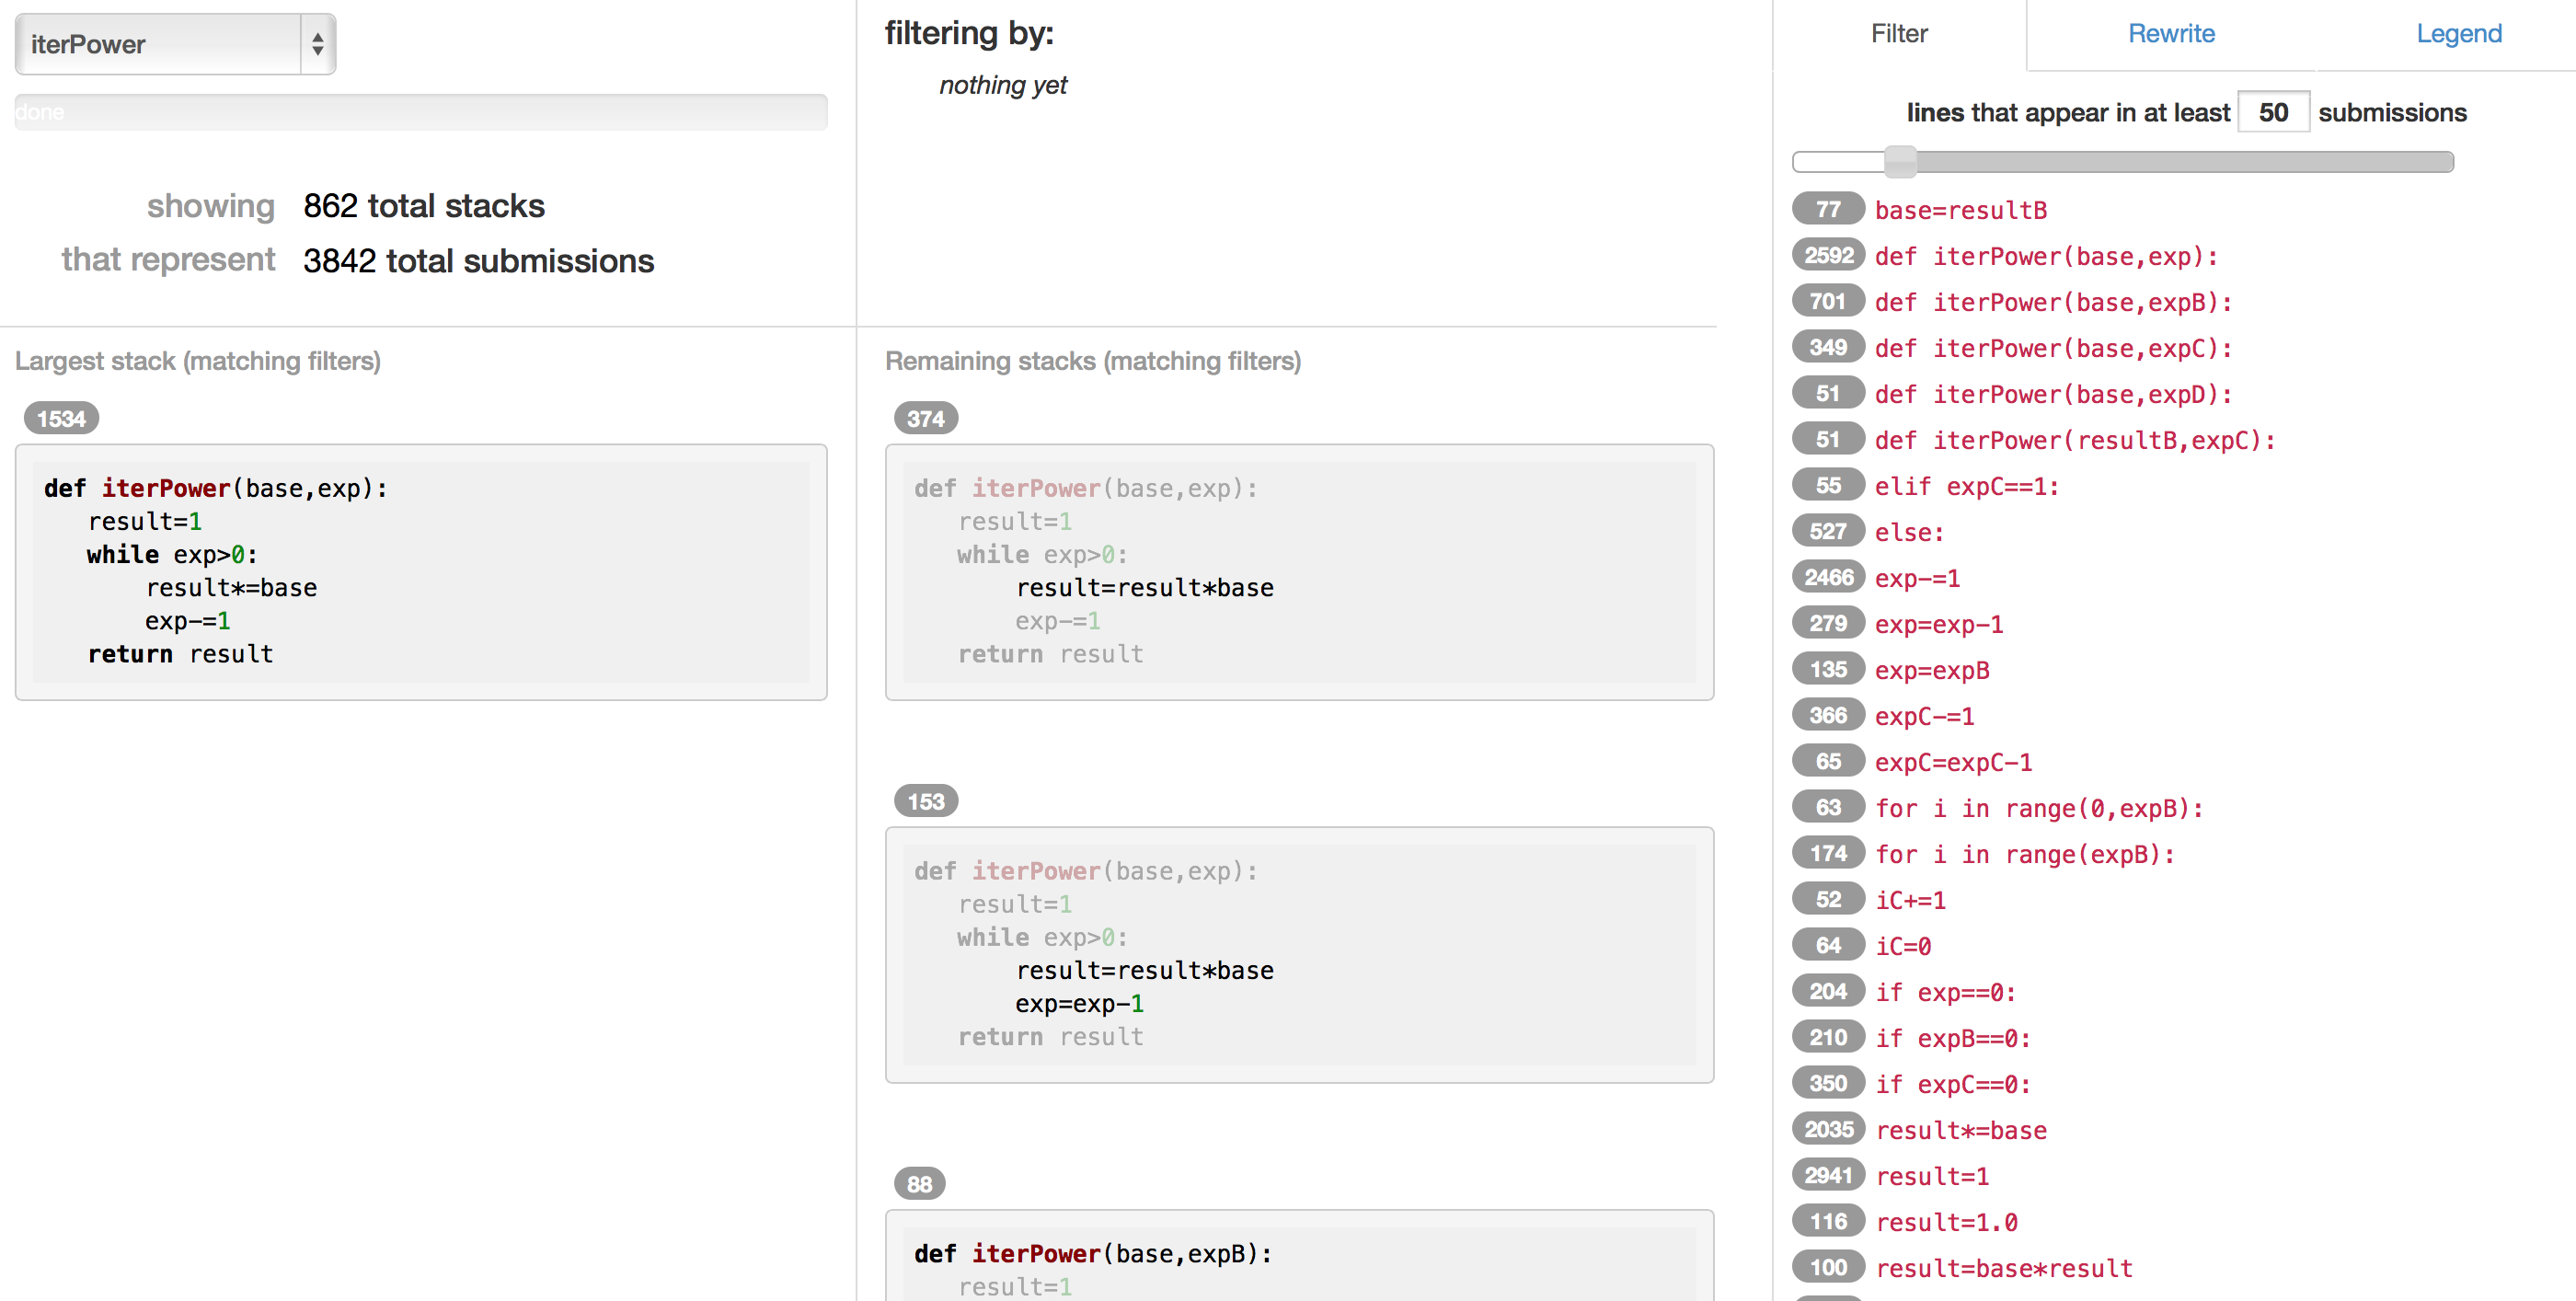
\includegraphics[width=1.0\linewidth]{Body/figures/overcode/interfaceScreenShot.png}
\caption{The OverCode user interface. The top left panel shows the number of clusters, called {\it stacks}, and the total number of solutions visualized. The next panel down in the first column shows the largest stack, while the second column shows the remaining stacks. The third column shows the lines of code \DIFdelbeginFL \DIFdelFL{occurring }\DIFdelendFL in the \DIFdelbeginFL \DIFdelFL{cleaned }\DIFdelendFL \DIFaddbeginFL \DIFaddFL{platonic }\DIFaddendFL solutions \DIFdelbeginFL \DIFdelFL{of the stacks together with }\DIFdelendFL \DIFaddbeginFL \DIFaddFL{and }\DIFaddendFL their frequencies.}
\label{overcode_fullinterface}
\end{figure*}

Sifting through thousands of solutions to understand their variation and find pedagogically valuable examples is a daunting task, even if the programming \DIFdelbegin \DIFdel{exercises }\DIFdelend \DIFaddbegin \DIFadd{problems }\DIFaddend are simple and the solutions are only tens of lines of code long. Without tool support, a teacher may not read more than 50-100 of them before growing frustrated with the tedium of the task. Given this small sample size, teachers cannot be expected to develop a thorough understanding of the variety of strategies used to solve the problem, \DIFdelbegin \DIFdel{or }\DIFdelend produce instructive feedback that is relevant to a large proportion of learners, or find unexpected interesting solutions.

An information visualization approach would enable teachers to explore the variation in solutions at scale. Existing techniques~\cite{gradingsigcse14,MOOCshop,codewebs} use a combination of clustering to group solutions that are semantically similar, and graph visualization to show the variation between these clusters. These clustering algorithms perform pairwise comparisons that are quadratic in both the number of solutions and in the size of each solution, which scales poorly to thousands of solutions. Graph visualization also struggles with how to label the graph node for a cluster, because it has been formed by a complex combination of code features. Without meaningful labels for clusters in the graph, the rich information \DIFdelbegin \DIFdel{of the learners' }\DIFdelend \DIFaddbegin \DIFadd{in student }\DIFaddend solutions is lost and the teacher's ability to understand variation is weakened.

\DIFdelbegin \DIFdel{In this paper we present }\DIFdelend \DIFaddbegin \DIFadd{This chapter presents }\DIFaddend OverCode, a system for visualizing and exploring the variation in thousands of programming solutions. OverCode is designed to visualize correct solutions, in the sense that they already passed the automatic grading tests typically used in a programming class at scale. The autograder cannot offer any further feedback on these correct solutions, and yet there may still be good and bad variations on correct solutions that are pedagogically valuable to highlight and discuss. OverCode aims to help teachers understand solution variation so that they can provide appropriate feedback to students at scale.

OverCode uses a novel \DIFdelbegin \DIFdel{clustering technique that creates clusters of identical cleaned code, in time linear in }\DIFdelend \DIFaddbegin \DIFadd{human-interpretable solution clustering technique. The clustering process is linear in time with respect to }\DIFaddend both the number of solutions and the size of each solution. The \DIFdelbegin \DIFdel{cleaned code }\DIFdelend \DIFaddbegin \DIFadd{platonic solution that represents each cluster }\DIFaddend is readable, executable, and describes every solution in that cluster \DIFdelbegin \DIFdel{.  The cleaned code is }\DIFdelend \DIFaddbegin \DIFadd{in a deterministic way that accounts for both syntax and behavior on test cases. The platonic solutions are }\DIFaddend shown in a visualization that puts code front-and-center (Figure~\ref{overcode_fullinterface}). In \DIFdelbegin \DIFdel{OverCode, the teacher reads through code }\DIFdelend \DIFaddbegin \DIFadd{the OverCode interface, teachers read through platonic }\DIFaddend solutions that each represent \DIFdelbegin \DIFdel{an entire cluster of solutionsthat look and act the same}\DIFdelend \DIFaddbegin \DIFadd{entire clusters of solutions}\DIFaddend . The differences between clusters are highlighted to help teachers discover and understand the variations among \DIFdelbegin \DIFdel{submitted }\DIFdelend solutions. Clusters can be filtered by the lines of code within them.  Clusters can also be merged together with {\em rewrite rules} that collapse variations that the teacher decides are unimportant. 

A cluster in OverCode is a set of solutions that perform the same computations, but may use different variable names or statement order.  OverCode uses a lightweight dynamic analysis to generate clusters, which scales linearly with the number of solutions. It clusters solutions whose variables take the same sequence of values when executed on test inputs and whose set of constituent lines of code are syntactically the same. 
\DIFaddbegin 

\DIFaddend An important component of this analysis is to rename variables that behave the same across different solutions. The renaming of variables serves three main purposes. First, it lets teachers create a mental mapping between variable names and their behavior which is consistent across the entire set of solutions. This may reduce the cognitive load for a teacher to understand different solutions. Second, it helps clustering by reducing variation between similar solutions. Finally, it also helps make the remaining differences between different solutions more salient. 

\DIFdelbegin \DIFdel{In }\DIFdelend \DIFaddbegin \DIFadd{This chapter concludes by presenting }\DIFaddend two user studies with a total of 24 participants who each looked at thousands of solutions from an introductory programming MOOC, \DIFdelbegin \DIFdel{we compared }\DIFdelend the OverCode interface \DIFaddbegin \DIFadd{is compared }\DIFaddend with a baseline interface that showed original unclustered solutions. When using OverCode, participants felt that they were able to develop a better high-level view of the students' understandings and misconceptions. While participants didn't necessarily read more lines of code in the OverCode interface than in the baseline, the code they did read came from clusters containing a greater percentage of all the submitted solutions. Participants also drafted mock class forum posts about common good and bad solutions\DIFdelbegin \DIFdel{that }\DIFdelend \DIFaddbegin \DIFadd{. These forum posts }\DIFaddend were relevant to more \DIFdelbegin \DIFdel{solutions (and the students who wrote them) }\DIFdelend \DIFaddbegin \DIFadd{student solutions }\DIFaddend when using OverCode as compared to the baseline. 

\section{OverCode} \label{overcode}
\DIFdelbegin \DIFdel{We now describe the OverCode user interface. OverCode }\DIFdelend \DIFaddbegin \DIFadd{OverCode }\DIFaddend is an information visualization application for teachers to explore student \DIFdelbegin \DIFdel{program solutions. The OverCode interface allows the user to scroll, filter, and }\emph{\DIFdel{stack}} %DIFAUXCMD
\DIFdel{solutions. OverCode }\DIFdelend \DIFaddbegin \DIFadd{solutions. OverCode }\DIFaddend uses the metaphor of \DIFdelbegin \DIFdel{stacks to denote collections }\DIFdelend \DIFaddbegin \DIFadd{solutions stacked on top of each other to denote a cluster }\DIFaddend of similar solutions\DIFdelbegin \DIFdel{, where each stack shows a }\emph{\DIFdel{cleaned}} %DIFAUXCMD
\DIFdel{solution from the corresponding collection of identical cleaned solutionsit represents. 
These cleaned solutions have strategically renamed variables and }\DIFdelend \DIFaddbegin \DIFadd{. The top solution in the stack is the platonic solution that represents all the other solutions in the stack. The OverCode interface allows the teacher to scroll through, filter, and merge stacks of solutions. 
}

\DIFadd{The platonic solutions that represent stacks are normalized in a novel way. Specifically, they have standardized formatting, no comments, and variable names that reflect the most popular naming choices across all solutions. They }\DIFaddend can be filtered by the \DIFdelbegin \DIFdel{cleaned }\DIFdelend \DIFaddbegin \DIFadd{normalized }\DIFaddend lines of code they contain \DIFdelbegin \DIFdel{. Cleaned solutions can also be rewritten when users compose andapply a }\emph{\DIFdel{rewrite rule}}%DIFAUXCMD
\DIFdel{, which can eliminate differences between cleaned solutions and therefore combine stacks of cleaned solutions that have become identical. }\DIFdelend \DIFaddbegin \DIFadd{and, through rewrite rules, modified and merged. They are the result of the normalization process applied to all student solutions in the OverCode analysis pipeline. %DIF > They can also be rewritten when teachers compose and apply \emph{rewrite rules}, which can eliminate differences between platonic solutions and therefore merge stacks that have become identical after the rewrite. 
}\DIFaddend 

\DIFdelbegin \DIFdel{We iteratively designed and developed the OverCode interface based on continuous evaluation by the authors, feedback from teachers and peers, and by consulting principles from the information visualization literature. }\DIFdelend %DIF > The OverCode interface was iteratively designed and developed based on continuous evaluation by the authors, feedback from teachers and peers, and by consulting principles from the information visualization literature. 
A screenshot of OverCode visualizing \codevar{iterPower}, one of the problems from our dataset, is shown in Figure~\ref{overcode_fullinterface}. In this section, \DIFdelbegin \DIFdel{we describe }\DIFdelend the intended use cases and the user interface \DIFaddbegin \DIFadd{are described}\DIFaddend . In Section \ref{pipeline}, the backend program analysis pipeline is described in detail. 
\DIFdelbegin %DIFDELCMD < \subsection{Target Users and Applications}
%DIFDELCMD < %%%
\DIFdelend \DIFaddbegin \subsection{Target Users and Tasks}
\DIFaddend The target users of OverCode are teaching staff of introductory programming courses. Teaching staff may be undergraduate lab assistants who help students debug their code; graduate students who grade assignments, help students debug, and manage recitations and course forums; and \DIFdelbegin \DIFdel{lecturing professors who also compose the }\DIFdelend \DIFaddbegin \DIFadd{instructors who compose }\DIFaddend major course assessments. Teachers using OverCode may be looking for common misconceptions, creating a grading rubric, or choosing pedagogically valuable examples to review with students in a future lesson.

\DIFdelbegin %DIFDELCMD < \subsubsection{Misconceptions and Holes in Students' Knowledge}
%DIFDELCMD < %%%
\DIFdelend \DIFaddbegin \subsubsection{Misconceptions and Holes in Student Knowledge}
\DIFaddend Students just starting to learn programming can have a difficult time understanding the language constructs and different API methods. They may use them suboptimally, or in non-standard ways. OverCode may help instructors identify these common misconceptions and holes in knowledge, by highlighting the differences between stacks of solutions. Since the visualized solutions have already been tested and found correct by an autograder, these highlighted differences between \DIFdelbegin \DIFdel{cleaned }\DIFdelend \DIFaddbegin \DIFadd{platonic }\DIFaddend solutions may be convoluted variations in construct usage and API method choices that have not been flagged by the Python interpreter or caused the failure of a unit test. Convoluted code may suggest a misconception.

\DIFaddbegin \todo{Rob: it would be great to show example code for these tasks, ideally showing them in OverCode -- can you mine any examples from your thesis defense talk?}

\DIFaddend \subsubsection{Grading Rubrics}
It is a difficult task to create grading rubrics for checking properties such as design and style of solutions. Therefore most autograders resort to checking only functional correctness of solutions by testing them against a test suite of input-output pairs. OverCode enables teachers to identify the style, structure, and relative frequency of the variation within correct solutions. Unlike traditional ways of creating a grading rubric, where an instructor may go through a set of solutions, revising the rubric along the way, instructors can use OverCode to first get a high-level overview of the variations before designing a corresponding rubric. Teachers may also see incorrect solutions not caught by the autograder.

\subsubsection{Pedagogically Valuable Examples} 
There can be a variety of ways to solve a given problem and express it in code. If an assignment allows students to generate different solutions, e.g., recursive or iterative, to fulfill the same input-output behavior, OverCode will show separate stacks for each of these different solutions, as well as stacks for every variant of those solutions. OverCode helps teachers filter through solutions to find different examples of solutions to the same problem, which may be pedagogically valuable. According to \DIFdelbegin \DIFdel{Variation Theory }\DIFdelend \DIFaddbegin \DIFadd{variation theory }\DIFaddend ~\cite{marton13}, students can learn through concrete examples of these multiple solutions, which vary along \DIFdelbegin \DIFdel{various }\DIFdelend \DIFaddbegin \DIFadd{different }\DIFaddend conceptual dimensions.
\subsection{User Interface}

The OverCode user interface is the product of an iterative design process with multiple stages, including paper prototypes and low-fidelity \DIFdelbegin \DIFdel{web-browser-based prototypes }\DIFdelend \DIFaddbegin \DIFadd{prototypes rendered in a web browser}\DIFaddend .  Prototype iterations were used and critiqued by members of our research group and by several teaching staff of an introductory Python programming course. While exploring the low-fidelity prototypes, these teachers talked aloud about their hopes for what the tool could do, frustrations with its current form, and their frustrations with existing solution-viewing tools and processes. This feedback was incorporated into the final design.

The OverCode user interface is divided into three columns. The top-left panel in the first column shows the problem name, the \emph{done} progress bar, the number of stacks, the number of visualized stacks given the current filters and rewrite rules, and the total number of solutions those visualized stacks contain. The panel below shows the largest stack \DIFdelbegin \DIFdel{that represents the most common solution}\DIFdelend \DIFaddbegin \DIFadd{of solutions}\DIFaddend . Side by side with the largest stack, the remaining \DIFdelbegin \DIFdel{solution }\DIFdelend stacks appear in the second panel. Through scrolling, any stack can be horizontally aligned with the largest stack for easier comparison. The third panel has three different tabs that provide static and dynamic information about the solutions, and the ability to filter and combine stacks. 

As shown in Figure~\ref{overcode_fullinterface}, the default tab shows a list of lines of code that occur in different \DIFdelbegin \DIFdel{cleaned }\DIFdelend \DIFaddbegin \DIFadd{platonic }\DIFaddend solutions together with their corresponding frequencies. The stacks can be filtered based on the occurrence of one or more lines (Filter tab). The column also has tabs for \emph{Rewrite} and \emph{Legend}. The Rewrite tab allows a teacher to provide rewrite rules to collapse different stacks with small differences into a larger single stack. The Legend tab shows the dynamic values that different program variables take during the execution of programs over a test case. \DIFdelbegin \DIFdel{We now describe different features of OverCode in more detail.
}\DIFdelend %DIF > We now describe different features of OverCode in more detail.
\DIFaddbegin \todo{ROB:maybe the TOCHI paper didn't have space for screenshots of these, but your thesis needs them}
\DIFaddend 

\subsubsection{Stacks} A stack in OverCode denotes a set of similar solutions that are grouped together based on a similarity criterion defined in Section \ref{pipeline}. For example, a stack for the \codevar{iterPower} problem is shown in Figure~\ref{stacks}(a). The size of each stack\DIFaddbegin \DIFadd{, i.e., the number of solutions in a stack, }\DIFaddend is shown in a pillbox at the top-left corner of the stack. \DIFdelbegin \DIFdel{The count denotes how many solutions are in the stack, and can also be referred to as the stack }%DIFDELCMD < {\it %%%
\DIFdel{size}%DIFDELCMD < }%%%
\DIFdel{. }\DIFdelend Stacks are listed in the scrollable second panel from largest to smallest. The solution on the top of the stack is a \DIFdelbegin \DIFdel{cleaned }\DIFdelend \DIFaddbegin \DIFadd{platonic }\DIFaddend solution that describes all the solutions in the stack. See Section \ref{pipeline} for details on the \DIFdelbegin \DIFdel{cleaning process }\DIFdelend \DIFaddbegin \DIFadd{normalizing process that produces platonic solutions}\DIFaddend .

Each stack can also be clicked. After clicking a stack, the border color of the stack changes and the \emph{done} progress bar is updated to reflect the percentage of total solutions clicked, as shown in Figure~\ref{stacks}(b). This feature is intended to help \DIFdelbegin \DIFdel{users }\DIFdelend \DIFaddbegin \DIFadd{teachers }\DIFaddend remember which stacks they have already read or analyzed, and keep track of their progress. Clicking on a large stack, which represents a significant fraction of the total solutions, is reflected by a large change in the \emph{done} progress bar. \todo{add that now the raw solutions inside the stack are also displayed, but this was not included during user study tests}

\begin{figure*}[htpb]
\begin{tabular}{c | c}
\begin{minipage}{.5\linewidth}
\centering
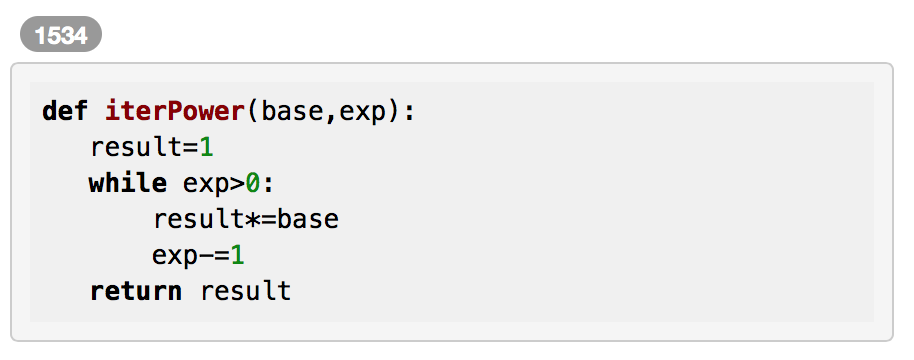
\includegraphics[width=0.95\linewidth]{Body/figures/overcode/stackScreenShot.png}
\end{minipage}
&
\begin{minipage}{.5\linewidth}
\centering
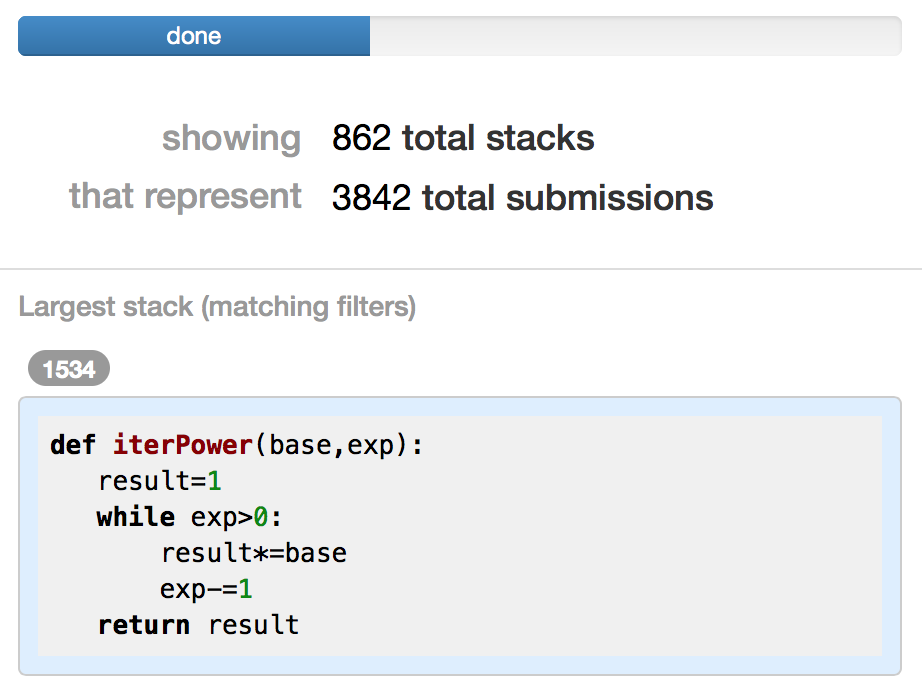
\includegraphics[width=0.95\linewidth]{Body/figures/overcode/checkDone.png}
\end{minipage}
\\
(a) & (b)
\end{tabular}
\caption{(a) A stack \DIFdelbeginFL \DIFdelFL{consisting }\DIFdelendFL of 1534 similar \codevar{iterPower} solutions. (b) After clicking a stack, the border color of the stack changes and the done progress bar denotes the corresponding fraction of solutions that have been checked.}
\label{stacks}
\end{figure*}

\subsubsection{Showing Differences between Stacks} OverCode allows teachers to compare smaller stacks, shown in the second column, with the largest stack, shown in the first column. The lines of code in the second column that also appear in the set of lines in the largest stack are dimmed so that only the differences between the smaller stacks and the largest stack are apparent. For example, Figure~\ref{stackdifferences} shows the differences between the \DIFdelbegin \DIFdel{cleaned }\DIFdelend \DIFaddbegin \DIFadd{platonic }\DIFaddend solutions of the two largest stacks. In earlier iterations of the user interface, lines in stacks that were not shared with the largest stack were highlighted in yellow, but this produced a lot of visual noise. By dimming the lines in stacks that \textit{are} shared with the largest stack, \DIFdelbegin \DIFdel{we reduced }\DIFdelend the visible noise \DIFaddbegin \DIFadd{is reduced}\DIFaddend , while still keeping differences between stacks salient.

\begin{figure*}
\centering
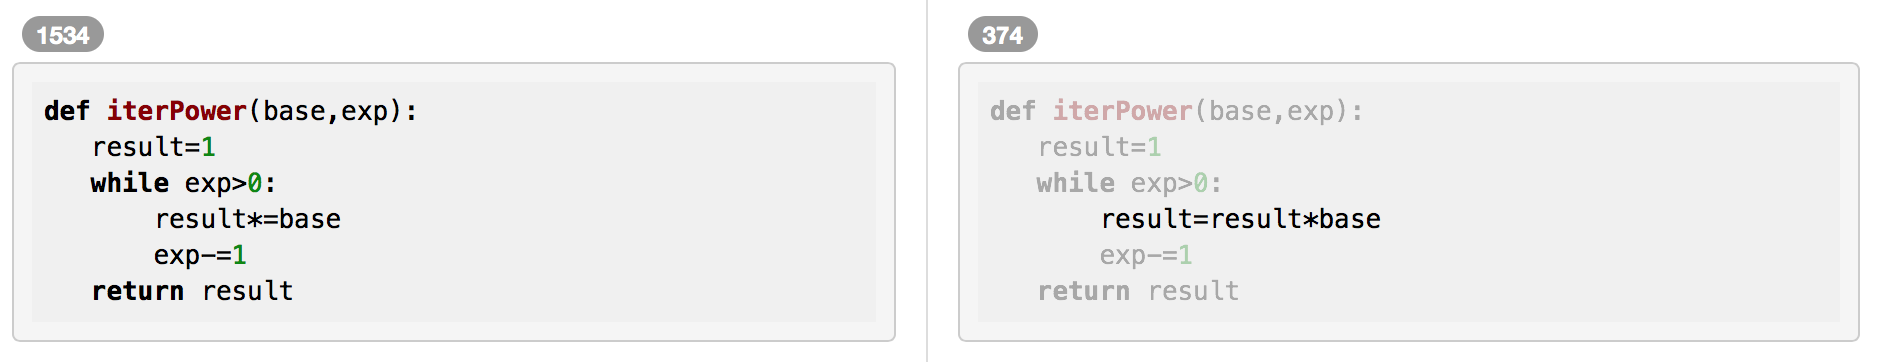
\includegraphics[scale=0.42]{Body/figures/overcode/lineFadingScreenshot}
\caption{Similar lines of code between two stacks are dimmed out such that only differences between the two stacks are apparent.}
\label{stackdifferences}
\end{figure*}



\subsubsection{Filtering Stacks by Lines of Code} The third column of OverCode shows the list of lines of code occurring in the solutions together with their frequencies (numbered pillboxes). The interface has a slider that can be used to change the threshold value, which denotes the number of solutions in which a line should appear for it to be included in the list. For example, by dragging the slider to $200$ in Figure~\ref{linefilter}(a), OverCode only shows lines of code that are present in at least $200$ solutions. This feature was added as a response to the length of the unfiltered list of code lines, which was long enough to make skimming for common code lines difficult.

Users can filter the stacks by selecting one or more lines of code from the list. After each selection, only stacks whose \DIFdelbegin \DIFdel{cleaned }\DIFdelend \DIFaddbegin \DIFadd{platonic }\DIFaddend solutions have those selected lines of code are shown. Figure~\ref{linefilter}(b) shows a filtering of stacks that have a \codevar{for} loop, specifically the line of code \codevar{for i in range(expB)}, and that assign $1$ to the variable \codevar{result}.

\begin{figure*}[htpb]
\begin{tabular}{c | c}
\begin{minipage}{.48\linewidth}
\centering
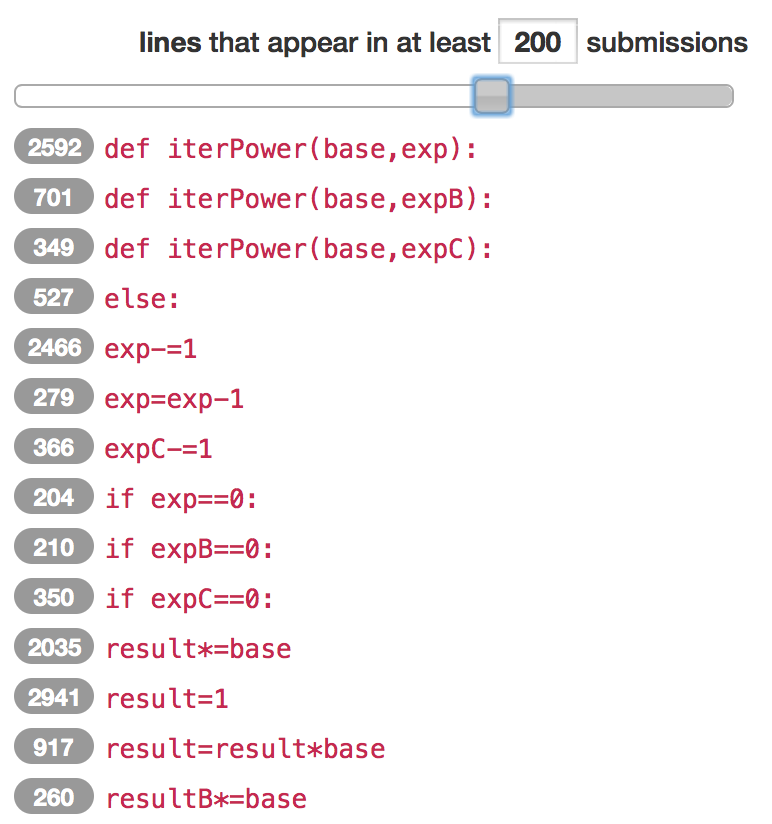
\includegraphics[scale=0.5]{Body/figures/overcode/lineSlider.png}
\end{minipage}
&
\begin{minipage}{.52\linewidth}
\centering
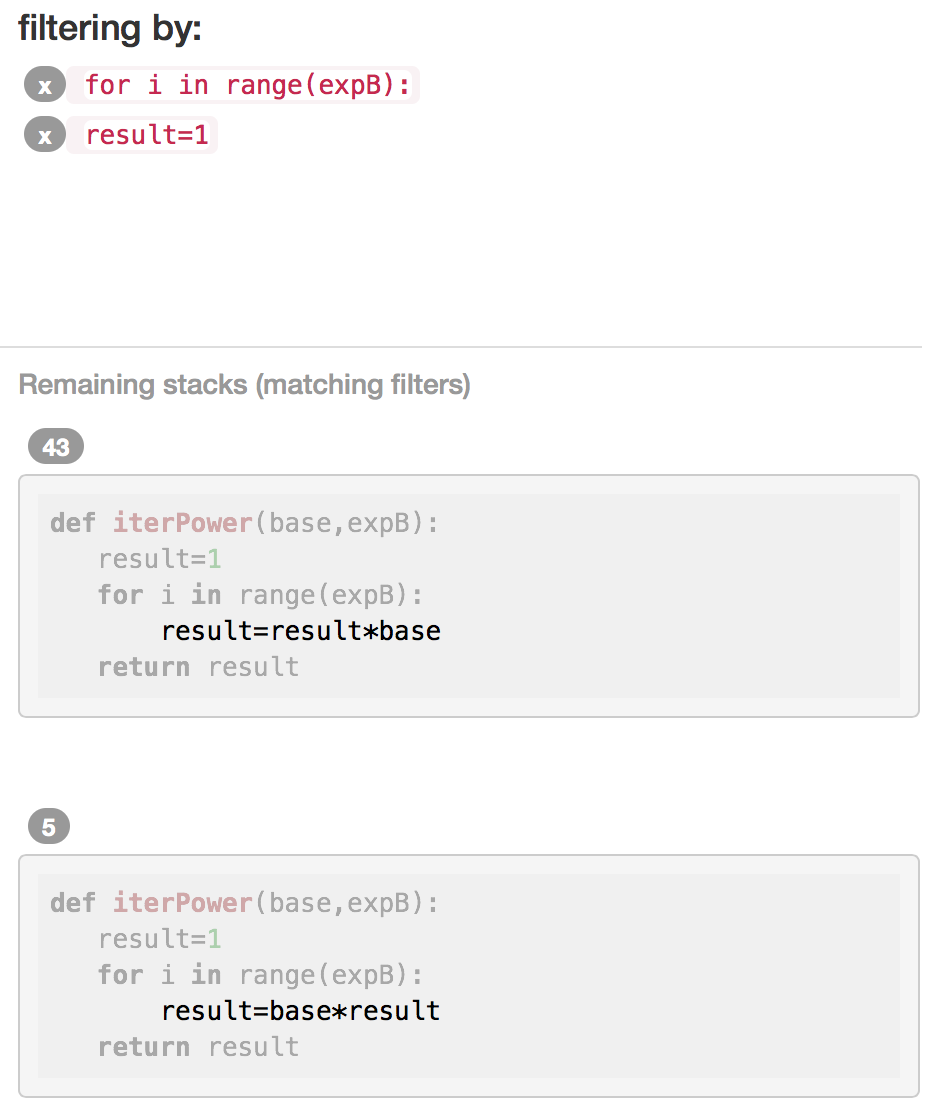
\includegraphics[scale=0.40]{Body/figures/overcode/lineFilter.png}
\end{minipage}
\\
(a) & (b)
\end{tabular}
\caption{(a) The slider allows filtering of the list of lines of code by the number of solutions in which they appear. (b) Clicking on a line of code adds it to the list of lines by which the stacks are filtered.}
\label{linefilter}
\end{figure*}

\subsubsection{Rewrite Rules} There are often small differences between the \DIFdelbegin \DIFdel{cleaned }\DIFdelend \DIFaddbegin \DIFadd{platonic }\DIFaddend solutions that can lead to a large number of stacks for a teacher to review. OverCode provides \emph{rewrite rules} by which \DIFdelbegin \DIFdel{users }\DIFdelend \DIFaddbegin \DIFadd{teachers }\DIFaddend can collapse these differences and ignore variation they do not need to see. This feature comes from experience with early prototypes. After observing a difference between stacks, like the use of \codevar{xrange} instead of \codevar{range}, \DIFdelbegin \DIFdel{users }\DIFdelend \DIFaddbegin \DIFadd{teachers }\DIFaddend wanted to ignore that difference in order to more easily find other differences.

A rewrite rule is described with a left hand side and a right hand side as shown in Figure~\ref{rewriterule}(a). The semantics of a rewrite rule is to replace all occurrences of the \DIFdelbegin \DIFdel{left hand }\DIFdelend \DIFaddbegin \DIFadd{left-hand }\DIFaddend side expression in the \DIFdelbegin \DIFdel{cleaned }\DIFdelend \DIFaddbegin \DIFadd{platonic }\DIFaddend solutions with the corresponding \DIFdelbegin \DIFdel{right hand }\DIFdelend \DIFaddbegin \DIFadd{right-hand }\DIFaddend side. As the rewrite rules are entered, OverCode presents a preview of the changes in the \DIFdelbegin \DIFdel{cleaned }\DIFdelend \DIFaddbegin \DIFadd{platonic }\DIFaddend solutions as shown in Figure~\ref{rewriterule}(b). After the application of the rewrite rules, OverCode collapses stacks that now have the same \DIFdelbegin \DIFdel{cleaned }\DIFdelend \DIFaddbegin \DIFadd{platonic }\DIFaddend solutions because of the rewrites. For example, after the application of the rewrite rule in Figure~\ref{rewriterule}(a), OverCode collapses the two biggest iterPower stacks from Figure~\ref{overcode_fullinterface} of sizes $1534$ and $374$, respectively, into a single stack of size $1908$. Other pairs of stacks whose differences have now been removed by the rewrite rule are also collapsed into single stacks. As shown in Figure~\ref{afterrewrite}(a), the number of stacks now drop from $862$ to $814$.

\begin{figure*}[htpb]
\begin{tabular}{c | c}
\begin{minipage}{.5\linewidth}
\centering
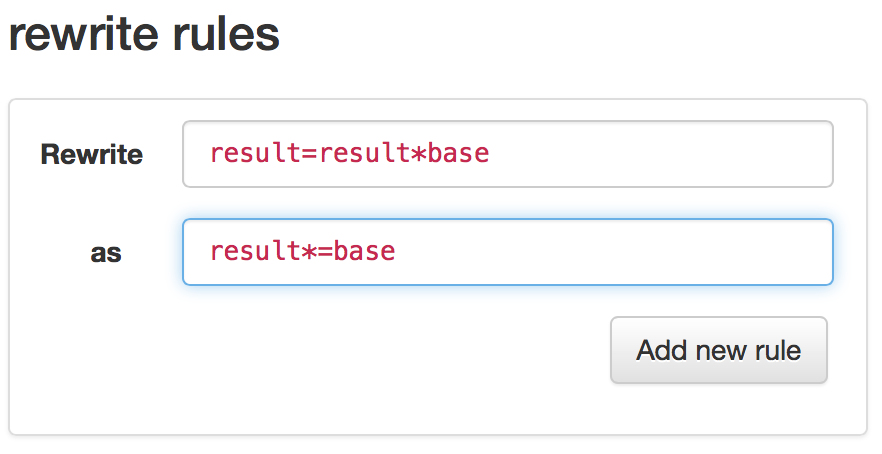
\includegraphics[scale=0.45]{Body/figures/overcode/rewriteRuleScreenshot.png}
\end{minipage}
&
\begin{minipage}{.5\linewidth}
\centering
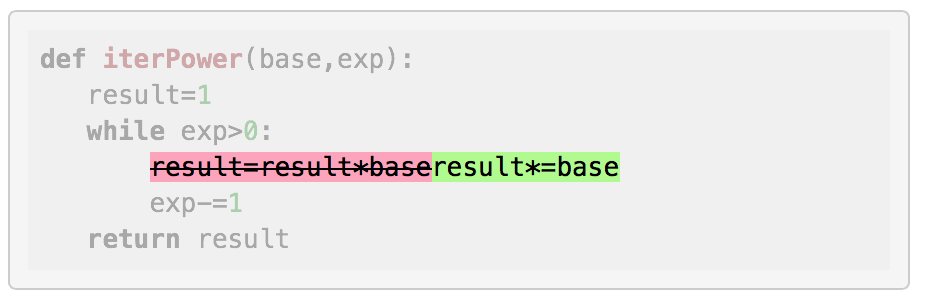
\includegraphics[scale=0.40]{Body/figures/overcode/rewritePreviewScreenShot.png}
\end{minipage}
\\
(a) & (b)
\end{tabular}
\caption{(a) An example rewrite rule to replace all occurrences of statement \codevar{result = base * result} with \codevar{result *= base}. (b) The preview of the changes in the \DIFdelbeginFL \DIFdelFL{cleaned }\DIFdelendFL \DIFaddbeginFL \DIFaddFL{platonic }\DIFaddendFL solutions because of the application of the rewrite rule.}
\label{rewriterule}
\end{figure*}

\begin{figure*}[htpb]
\begin{tabular}{c | c}
\begin{minipage}{.5\linewidth}
\centering
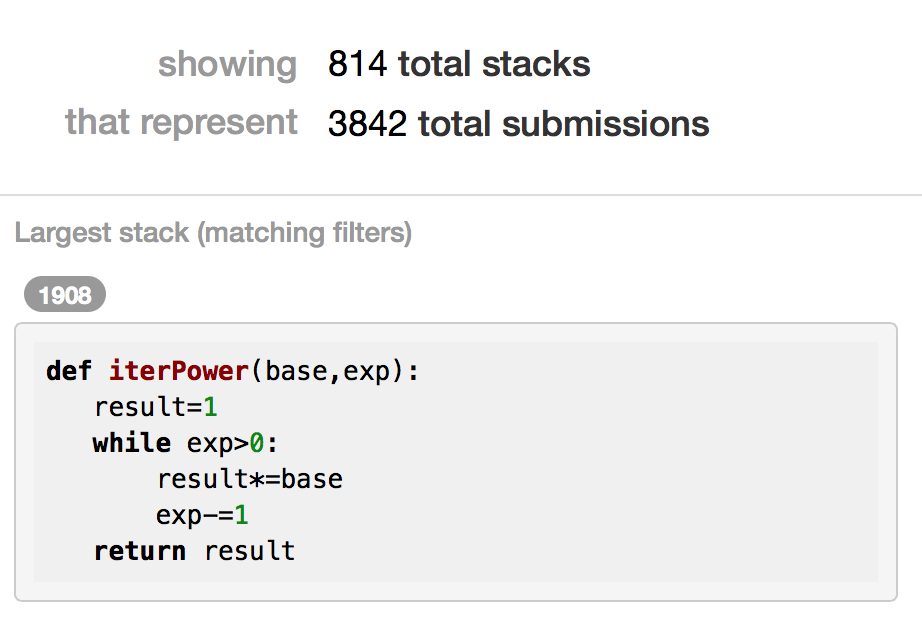
\includegraphics[scale=0.4]{Body/figures/overcode/afterrewrite.png}
\end{minipage}
&
\begin{minipage}{.5\linewidth}
\centering
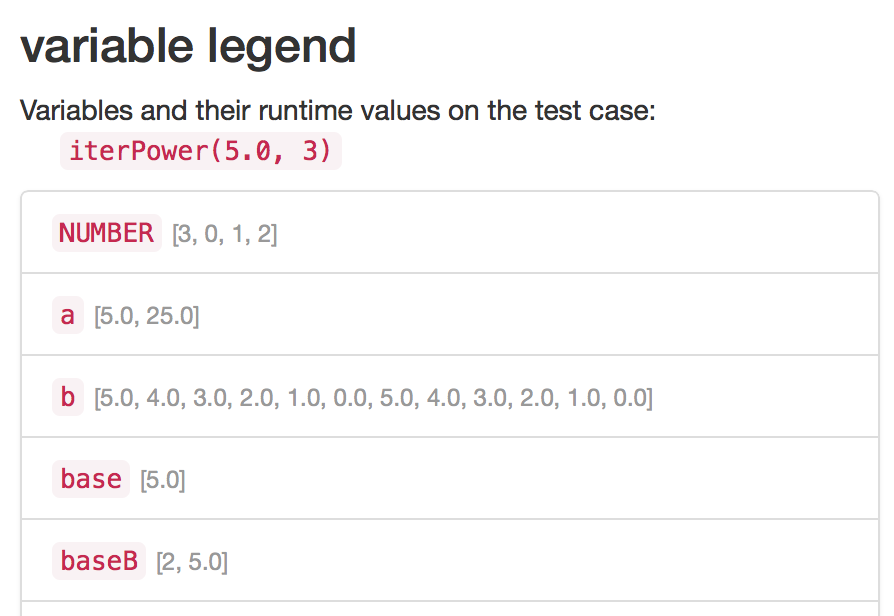
\includegraphics[scale=0.4]{Body/figures/overcode/variableLegend.png}
\end{minipage}
\\
(a) & (b)
\end{tabular}
\caption{(a) The merging of stacks after application of the rewrite rule shown in Figure~\ref{rewriterule}. (b) The variable legend shows the sequence of dynamic values that all program variables in \DIFdelbeginFL \DIFdelFL{cleaned }\DIFdelendFL \DIFaddbeginFL \DIFaddFL{normalized }\DIFaddendFL solutions take over the course of execution on a given test case.}
\label{afterrewrite}
\end{figure*}

\subsubsection{Variable Legends} OverCode also shows the sequence of values that variables in the \DIFdelbegin \DIFdel{cleaned }\DIFdelend \DIFaddbegin \DIFadd{platonic }\DIFaddend solutions take on, over the course of their execution on a test case. As described in Section~\ref{pipeline}, a variable is identified by the sequence of values it takes on during the execution of the test case. Figure~\ref{afterrewrite}(b) shows a snapshot of the variable values for the \codevar{iterPower} problem. The goal of presenting this dynamic information associated with common variable names is \DIFdelbegin \DIFdel{to help users }\DIFdelend \DIFaddbegin \DIFadd{intended to help teachers (1) }\DIFaddend understand the behavior of each \DIFdelbegin \DIFdel{cleaned solution , and }\DIFdelend \DIFaddbegin \DIFadd{platonic solution without having to mentally execute it on a test case and (2) }\DIFaddend further explore the variations among solutions that do not have the same common variables. When this legend was originally added to the user interface, clicking on a common variable name would filter for all solutions that contained an instance of that variable. Some pilot users found this feature confusing, rather than empowering. As a result, it was removed from OverCode before running both user studies. At least one study participant, upon realizing the value of the legend, wished that the original click-to-filter-by-variable functionality existed; it may be \DIFdelbegin \DIFdel{re-instated }\DIFdelend \DIFaddbegin \DIFadd{reinstated }\DIFaddend in future versions.

\section{Implementation} \label{pipeline}
The OverCode user interface depends on an analysis pipeline that \DIFdelbegin \DIFdel{canonicalizes }\DIFdelend \DIFaddbegin \DIFadd{normalizes }\DIFaddend solutions in a manner designed for human readability\DIFdelbegin \DIFdel{, referred to here as }\emph{\DIFdel{cleaning}}%DIFAUXCMD
\DIFdelend . The pipeline then creates stacks of solutions that have become identical through the \DIFdelbegin \DIFdel{cleaning }\DIFdelend \DIFaddbegin \DIFadd{normalizing }\DIFaddend process. The pipeline accepts, as input, a set of solutions, expressed as function definitions for $f(a,...)$, and \DIFdelbegin \DIFdel{one test case $f(a_{1},...)$. We refer to the solutions }\DIFdelend \DIFaddbegin \DIFadd{a set of test cases. Solutions }\DIFaddend that enter the pipeline \DIFaddbegin \DIFadd{are referred to }\DIFaddend as \emph{raw}, and the solutions that exit the pipeline as \emph{\DIFdelbegin \DIFdel{clean}\DIFdelend \DIFaddbegin \DIFadd{normal}\DIFaddend }. \DIFdelbegin \DIFdel{To illustrate this pipeline, we will have a few running examples, }\DIFdelend \DIFaddbegin \DIFadd{Examples, }\DIFaddend beginning with \codevar{iterPower}\DIFaddbegin \DIFadd{, are presented below to illustrate this pipeline}\DIFaddend .

\subsection{Analysis Pipeline}
OverCode is currently implemented for Python, but the pipeline steps described below could be readily generalized to other languages commonly used to teach programming.

{\bf 1. Reformat solutions.} For a consistent appearance, the solutions are reformatted \DIFaddbegin \DIFadd{with the PythonTidy package}\DIFaddend \footnote{\DIFdelbegin \DIFdel{We used the PythonTidy package, }\DIFdelend \DIFaddbegin \DIFadd{Created }\DIFaddend by Charles Curtis Rhode. \url{https://pypi.python.org/pypi/PythonTidy/}\DIFdelbegin \DIFdel{Since our datasets are in Python, we use a Python-specific reformatting script. However, our approach is not language-specific.}\DIFdelend } to have consistent line indentation and token spacing. Comments and empty lines are also removed. These steps not only make solutions more readable, but also allow exact string matches between solutions, after additional \DIFdelbegin \DIFdel{cleaning }\DIFdelend \DIFaddbegin \DIFadd{normalizing }\DIFaddend steps later in the pipeline. Although comments can contain valuable information, the variation in comments is so great that clustering and summarizing them will require significant additional design, which remains future work. \DIFdelbegin %DIFDELCMD < 

%DIFDELCMD < %%%
\DIFdel{The following example }\DIFdelend \DIFaddbegin \DIFadd{Figure~\ref{fig:reformat} }\DIFaddend illustrates the effect of this reformatting\DIFdelbegin \DIFdel{:
}%DIFDELCMD < 

%DIFDELCMD < \begin{tabular}{cc}
%DIFDELCMD < %%%
\DIFdelend \DIFaddbegin \DIFadd{.
}\begin{figure}
\begin{tabular}{ll}
\DIFaddendFL {\bf Student A Raw Code} & {\bf Student A Reformatted} \\
\begin{minipage}{0.5\linewidth}
\DIFdelbeginFL %DIFDELCMD < \begin{lstlisting}[language=python]
%DIFDELCMD < %%%
\DIFdelendFL \DIFaddbeginFL \begin{lstlisting}[basicstyle=\linespread{1.0}\ttfamily\footnotesize,language=python]
\DIFaddendFL def iterPower(base, exp):
    '''
    base: int or float.
    exp: int >= 0
    returns: int or float, base^exp
    '''
    result = 1
    for i in range(exp):
        result *= base
    return result
\end{lstlisting}
\end{minipage}
&
\begin{minipage}{0.5\linewidth}
\DIFdelbeginFL %DIFDELCMD < \begin{lstlisting}[language=python]
%DIFDELCMD < %%%
\DIFdelendFL \DIFaddbeginFL \begin{lstlisting}[basicstyle=\linespread{1.0}\ttfamily\footnotesize,language=python]
\DIFaddendFL def iterPower(base,exp):
    result=1
    for i in range(exp):
        result*=base
    return result
\end{lstlisting}
\end{minipage}
\end{tabular}
\DIFaddbeginFL \caption{\DIFaddFL{A student solution before and after reformatting.}}
\label{fig:reformat}
\end{figure}
\DIFaddend 

{\bf 2. Execute solutions.} Each solution is \DIFdelbegin \DIFdel{executed once, using }\DIFdelend \DIFaddbegin \DIFadd{on }\DIFaddend the same test case\DIFaddbegin \DIFadd{(s)}\DIFaddend . During each step of the execution \DIFaddbegin \DIFadd{for each test case}\DIFaddend , the names and values of local and global variables, and also return values from functions, are recorded as a program trace \DIFaddbegin \DIFadd{using an adaptation of Philip Guo's logger~\mbox{%DIFAUXCMD
\cite{pgbovineOPT}}%DIFAUXCMD
}\DIFaddend . There is one program trace per solution \DIFdelbegin \DIFdel{. For the purposes }\DIFdelend \DIFaddbegin \DIFadd{per test case. Included for the purpose }\DIFaddend of illustrating this pipeline, \DIFdelbegin \DIFdel{we will use the example of }\DIFdelend \DIFaddbegin \DIFadd{the examples in the figures that follow are derived from }\DIFaddend executing definitions of \codevar{iterPower} on a \codevar{base} of $5.0$ and an \codevar{exp} of $3$\DIFdelbegin \DIFdel{. }%DIFDELCMD < \\
%DIFDELCMD < 

%DIFDELCMD < %%%
\DIFdelend \DIFaddbegin \DIFadd{, as illustrated in Figure~\ref{fig:testcase}.
}\begin{figure}
\begin{tabular}{l}
\DIFaddendFL {\bf Student Code with Test Case} \\
\begin{minipage}{0.5\linewidth}
\DIFdelbeginFL %DIFDELCMD < \begin{lstlisting}[language=python]
%DIFDELCMD < %%%
\DIFdelendFL \DIFaddbeginFL \begin{lstlisting}[basicstyle=\linespread{1.0}\ttfamily\footnotesize,language=python]
\DIFaddendFL def iterPower(base,exp):
    #student code here
iterPower(5.0, 3)
\end{lstlisting}
\end{minipage} 
\DIFdelbeginFL %DIFDELCMD < \\
%DIFDELCMD < %%%
\DIFdelendFL \DIFaddbeginFL \end{tabular}
\caption{\DIFaddFL{Illustration of running a (dummy) }\texttt{\DIFaddFL{iterPower}} \DIFaddFL{solution on a test case.}}
\label{fig:testcase}
\end{figure}
\DIFaddend 

{\bf 3. Extract variable sequences.} \DIFdelbegin \DIFdel{During the previous step, the Python execution logger \mbox{%DIFAUXCMD
\cite{pgbovineOPT} }%DIFAUXCMD
records the values of all in-scope variables after every statement execution in the Python program. The resulting log is referred to as the program trace. }\DIFdelend For each variable in a program trace, \DIFdelbegin \DIFdel{we extract the sequence of }\DIFdelend \DIFaddbegin \DIFadd{the pipeline extracts the sequence of distinct }\DIFaddend values it takes on\DIFaddbegin \DIFadd{. Figure~\ref{fig:extractsequence} shows the program trace for a solution run on a test case, as well as the extracted sequences of distinct values for each variable. Variable sequence extraction also works for purely functional programs, in which variables are never reassigned, because each recursive invocation is treated as if new values are given to its parameter variables. For example, in spite of the fact that the }\codevar{iterPower} \DIFadd{problem asked students to compute the exponential $\codevar{base}^\codevar{exp}$ }\textit{\DIFadd{iteratively}}\DIFaddend , \DIFdelbegin \DIFdel{without considering how many statements were executed before the variable 's value changed.
}%DIFDELCMD < \\
%DIFDELCMD < \begin{tabular}{cc}
%DIFDELCMD < %%%
\DIFdelend \DIFaddbegin \DIFadd{$60$ of the $3842$ }\codevar{iterPower} \DIFadd{solutions in the dataset were in fact recursive. One of these recursive examples is shown in Figure~\ref{fig:recursiveTrace}, along with the variable sequences extracted.
}\begin{figure}
\begin{tabular}{ll}
\DIFaddendFL {\bf Student A Code with Test Case} & {\bf Program Trace for Student A Code} \\
\begin{minipage}{0.35\linewidth}
\DIFdelbeginFL %DIFDELCMD < \begin{lstlisting}[language=python]
%DIFDELCMD < %%%
\DIFdelendFL \DIFaddbeginFL \begin{lstlisting}[basicstyle=\linespread{1.0}\ttfamily\footnotesize,language=python]
\DIFaddendFL def iterPower(base,exp):
    result=1
    for i in range(exp):
        result*=base
    return result
iterPower(5.0, 3)
\end{lstlisting}
\end{minipage} &
\begin{minipage}{0.6\linewidth}
\begin{lstlisting}[\DIFaddbeginFL \DIFaddFL{basicstyle=}\linespread{1.0}\ttfamily\footnotesize\DIFaddFL{,}\DIFaddendFL language=python,linebackgroundcolor={\DIFdelbeginFL %DIFDELCMD < \lstcolorlines[lightyellow]{2,4,6,8,10,12,14,16,18}%%%
\DIFdelendFL \DIFaddbeginFL \lstcolorlines[gray!20]{2,4,6,8,10,12,14,16,18}\DIFaddendFL }]
iterPower(5.0, 3)
 base : 5.0, exp : 3
result=1
 base : 5.0, exp : 3, result : 1 
for i in range(exp):
 base : 5.0, exp : 3, result : 1, i : 0
result*=base
 base : 5.0, exp : 3, result : 5.0, i : 0 
for i in range(exp):
 base : 5.0, exp : 3, result : 5.0, i : 1
result*=base 
 base : 5.0, exp : 3, result : 25.0, i : 1 
for i in range(exp):
 base : 5.0, exp : 3, result : 25.0, i : 2 
result*=base
 base : 5.0, exp : 3, result : 125.0, i : 2
return result
 value returned: 125.0
\end{lstlisting}
\end{minipage} 
\\
& {\bf Variable Sequences for Student A Code} \\
&
\begin{minipage}{0.6\linewidth}
\begin{lstlisting}[language=python]
base: 5.0
exp: 3
result: 1, 5.0, 25.0, 125.0
i: 0, 1, 2
\end{lstlisting}
\end{minipage}
\DIFdelbeginFL %DIFDELCMD < \\
%DIFDELCMD < %%%
\DIFdelendFL \end{tabular}
\DIFaddbeginFL \caption{\DIFaddFL{A student solution, its program trace when running on the test case }\texttt{\DIFaddFL{iterPower(5.0,3)}}\DIFaddFL{, and the sequence of values extracted from the trace for each variable.}}
\label{fig:extractsequence}
\end{figure}
\DIFaddend 

\DIFdelbegin \DIFdel{Variable sequence extraction also works for purely functional programs, in which variables are never reassigned, because each recursive invocation is treated as if new values are given to its parameter variables. For example, in spite of the fact that the }%DIFDELCMD < \codevar{iterPower} %%%
\DIFdel{problem asked students to compute the exponential $\codevar{base}^\codevar{exp}$ }\textit{\DIFdel{iteratively}}%DIFAUXCMD
\DIFdel{, $60$ of the $3842$ }%DIFDELCMD < \codevar{iterPower} %%%
\DIFdel{solutions in the dataset were in fact recursive. One of these recursive examples is shown below, along with the variable sequences observed for the recursive function's parameters.
}%DIFDELCMD < 

%DIFDELCMD < \begin{tabular}{cc}
%DIFDELCMD < %%%
\DIFdelend \DIFaddbegin \begin{figure}
\begin{tabular}{ll}
\DIFaddendFL {\bf Recursive Example} & {\bf Program Trace\DIFdelbeginFL \DIFdelFL{for Recursive Example}\DIFdelendFL } \\
 %DIF >  & {\bf for Recursive Example} \\
\begin{minipage}{0.5\linewidth}
\DIFdelbeginFL %DIFDELCMD < \begin{lstlisting}[language=python]
%DIFDELCMD < %%%
\DIFdelendFL \DIFaddbeginFL \begin{lstlisting}[basicstyle=\linespread{1.0}\ttfamily\footnotesize,language=python]
\DIFaddendFL def iterPower(base,exp):
   if exp==0:
       return 1
   else:
       return base*iterPower(base,exp-1)
iterPower(5.0, 3)
\end{lstlisting}
\end{minipage} &
\DIFdelbeginFL %DIFDELCMD < \begin{minipage}{0.5\linewidth}
%DIFDELCMD < \begin{lstlisting}[language=python]
%DIFDELCMD < %%%
\DIFdelendFL \DIFaddbeginFL \begin{minipage}{0.4\linewidth}
\begin{lstlisting}[\DIFaddFL{basicstyle=}\linespread{1.0}\ttfamily\footnotesize\DIFaddFL{,language=python,linebackgroundcolor=}{\lstcolorlines[gray!20]{2,4,6,8,10,12,14,16,18,20,22,24,26,28,30}}]
\DIFaddendFL iterPower(5.0, 3)
 base : 5.0, exp : 3
if exp==0:
 base : 5.0, exp : 3 
return base*iterPower(base,exp-1)
 base : 5.0, exp : 3 
iterPower(5.0, 2)
 base : 5.0, exp : 2
if exp==0: 
 base : 5.0, exp : 2 
return base*iterPower(base,exp-1)
 base : 5.0, exp : 2
iterPower(5.0, 1)
 base : 5.0, exp : 1
if exp==0:
 base : 5.0, exp : 1
return base*iterPower(base,exp-1)
 base : 5.0, exp : 1
iterPower(5.0, 0)
 base : 5.0, exp : 0
if exp==0:
 base : 5.0, exp : 0
return 1
 base : 5.0, exp : 0
return base*1
 base : 5.0, exp : 1
return base*5
 base : 5.0, exp : 2
return base*25
 base : 5.0, exp : 3
value returned: 125.0
\end{lstlisting}
\end{minipage} 
\\
& {\bf Variable Sequences\DIFdelbeginFL \DIFdelFL{for Recursive Example}\DIFdelendFL } \\
%DIF >  & {\bf for Recursive Example} \\
&
\begin{minipage}{0.5\linewidth}
\begin{lstlisting}[language=python]
base: 5.0
exp: 3, 2, 1, 0, 1, 2, 3
\end{lstlisting}
\end{minipage}
\DIFdelbeginFL %DIFDELCMD < \\
%DIFDELCMD < %%%
\DIFdelendFL \end{tabular}
\DIFaddbeginFL \caption{\DIFaddFL{A recursive solution to the same programming problem, its program trace when executing on }\texttt{\DIFaddFL{iterPower(5.0,3)}}\DIFaddFL{, and the extracted sequences of values for each variable.}}
\label{fig:recursiveTrace}
\end{figure}
\DIFaddend 


{\bf 4. Identify common variables.} \DIFdelbegin \DIFdel{We analyze }\DIFdelend \DIFaddbegin \DIFadd{The pipeline analyzes }\DIFaddend all program traces, identifying which variables' sequences are identical. \DIFdelbegin \DIFdel{We define a }%DIFDELCMD < {\it %%%
\DIFdel{common variable}%DIFDELCMD < } %%%
\DIFdel{to denote those variables }\DIFdelend \DIFaddbegin \DIFadd{Variables }\DIFaddend that have identical sequences across two or more program traces \DIFaddbegin \DIFadd{are referred to as }{\it \DIFadd{common variables}}\DIFaddend . Variables which occur in only one program trace are called {\it unique variables}. \DIFdelbegin %DIFDELCMD < 

%DIFDELCMD < \begin{tabular}{cc}
%DIFDELCMD < %%%
\DIFdelend \DIFaddbegin \DIFadd{This is illustrated in Figures~\ref{fig:commik} and~\ref{fig:allvars}.
}\begin{figure}
\begin{tabular}{ll}
\DIFaddendFL {\bf Student B Code with Test Case} & {\bf Variable Sequences for Student B Code} \\
\begin{minipage}{0.5\linewidth}
\DIFdelbeginFL %DIFDELCMD < \begin{lstlisting}[language=python]
%DIFDELCMD < %%%
\DIFdelendFL \DIFaddbeginFL \begin{lstlisting}[basicstyle=\linespread{1.0}\ttfamily\footnotesize,language=python]
\DIFaddendFL def iterPower(base,exp):
    r=1
    for k in xrange(exp):
        r=r*base
    return r
iterPower(5.0, 3)
\end{lstlisting}
\end{minipage}
&
\begin{minipage}{0.5\linewidth}
\begin{lstlisting}[language=python]
base: 5.0
exp: 3
r: 1, 5.0, 25.0, 125.0
k: 0, 1, 2
\end{lstlisting}
\end{minipage} \\
{\bf Student C Code with Test Case} & {\bf Variable Sequences for Student C Code} \\
\begin{minipage}{0.5\linewidth}
\DIFdelbeginFL %DIFDELCMD < \begin{lstlisting}[language=python]
%DIFDELCMD < %%%
\DIFdelendFL \DIFaddbeginFL \begin{lstlisting}[basicstyle=\linespread{1.0}\ttfamily\footnotesize,language=python]
\DIFaddendFL def iterPower(base,exp):
   result=1
   while exp>0:
       result*=base
       exp-=1
   return result
iterPower(5.0, 3)
\end{lstlisting}
\end{minipage}
&
\begin{minipage}{0.5\linewidth}
\begin{lstlisting}[language=python]
base : 5.0
exp: 3
result : 1, 5.0, 25.0, 125.0
exp : 3, 2, 1, 0
\end{lstlisting}
\end{minipage}
\DIFdelbeginFL %DIFDELCMD < \\
%DIFDELCMD < %%%
\DIFdelendFL \end{tabular}
\DIFdelbeginFL %DIFDELCMD < 

%DIFDELCMD < %%%
\DIFdelFL{For example, in Student A's code and Student B's code, }%DIFDELCMD < \codevar{i} %%%
\DIFdelFL{and }%DIFDELCMD < \codevar{k} %%%
\DIFdelFL{take on the same sequence of values: $0$,$1$,$2$. They are therefore considered the same }\DIFdelendFL \DIFaddbeginFL \caption{\codevar{i} \DIFaddFL{and }\codevar{k} \DIFaddFL{take on the same sequence of values in Student A's and Student B's code: $0$,$1$,$2$. They are therefore considered the same }{\it \DIFaddFL{common variable}}\DIFaddFL{.}}
\label{fig:commik}
\end{figure}
\begin{figure}
\DIFaddendFL {\DIFdelbeginFL %DIFDELCMD < \it %%%
\DIFdelFL{common variable}%DIFDELCMD < }%%%
\DIFdelFL{.
}%DIFDELCMD < 

%DIFDELCMD < \begin{tabular}{cc}
%DIFDELCMD < {%%%
\DIFdelendFL \bf Common \DIFdelbeginFL \DIFdelFL{Variables}\DIFdelendFL \DIFaddbeginFL \DIFaddFL{variables}\DIFaddendFL } \DIFdelbeginFL %DIFDELCMD < & {\bf  %%%
\DIFdelFL{Unique Variables}%DIFDELCMD < } \\
%DIFDELCMD < %%%
\DIFdelFL{(across }\DIFdelendFL \DIFaddbeginFL \DIFaddFL{in }\DIFaddendFL Students A, B, and C\DIFdelbeginFL \DIFdelFL{) }%DIFDELCMD < & %%%
\DIFdelFL{(across Students A, B, and C) }%DIFDELCMD < \\
%DIFDELCMD < \begin{minipage}{0.5\linewidth}
%DIFDELCMD < %%%
\DIFdelendFL \DIFaddbeginFL \DIFaddFL{'s code:
}\DIFaddendFL  \begin{itemize} 
\item \texttt{5.0}:
\DIFdelbeginFL %DIFDELCMD < 

%DIFDELCMD < %%%
\DIFdelendFL \DIFaddbeginFL  \begin{itemize} 
\item \DIFaddendFL \texttt{base} (Students A, B, C)
\DIFaddbeginFL  \end{itemize} 
\DIFaddendFL \item \texttt{3}:
\DIFdelbeginFL %DIFDELCMD < 

%DIFDELCMD < %%%
\DIFdelendFL \DIFaddbeginFL  \begin{itemize} 
\item \DIFaddendFL \texttt{exp} (Students A, B) 
\DIFaddbeginFL  \end{itemize} 
\DIFaddendFL \item \texttt{1, 5.0, 25.0, 125.0}: 
\DIFdelbeginFL %DIFDELCMD < 

%DIFDELCMD < %%%
\DIFdelendFL \DIFaddbeginFL  \begin{itemize} 
\item \DIFaddendFL \texttt{result} (Students A, C)
\DIFdelbeginFL %DIFDELCMD < 

%DIFDELCMD < %%%
\DIFdelendFL \DIFaddbeginFL \item \DIFaddendFL \texttt{r} (Student B)
\DIFaddbeginFL  \end{itemize} 
\DIFaddendFL \item \texttt{0,1,2}:
\DIFdelbeginFL %DIFDELCMD < 

%DIFDELCMD < %%%
\DIFdelendFL \DIFaddbeginFL  \begin{itemize} 
\item \DIFaddendFL \texttt{i} (Student A) 
\DIFdelbeginFL %DIFDELCMD < 

%DIFDELCMD < %%%
\DIFdelendFL \DIFaddbeginFL \item \DIFaddendFL \texttt{k} (Student B)
 \end{itemize} 
\DIFdelbeginFL %DIFDELCMD < \end{minipage}
%DIFDELCMD < &
%DIFDELCMD < \begin{minipage}{0.5\linewidth}
%DIFDELCMD < %%%
\DIFdelendFL \DIFaddbeginFL  \end{itemize} 
{\bf \DIFaddFL{Unique variables}} \DIFaddFL{in Students A, B, and C's code:
}\DIFaddendFL  \begin{itemize} 
\item \texttt{3,2,1,0}:
\DIFdelbeginFL %DIFDELCMD < 

%DIFDELCMD < %%%
\DIFdelendFL \DIFaddbeginFL  \begin{itemize} 
\item \DIFaddendFL \texttt{exp} (Student C)
 \end{itemize} 
\DIFdelbeginFL %DIFDELCMD < \end{minipage} \\
%DIFDELCMD < \end{tabular}
%DIFDELCMD < %%%
\DIFdelendFL \DIFaddbeginFL  \end{itemize} 
\caption{\DIFaddFL{Common and uncommon variables found across the solutions in the previous figure.}}
\label{fig:allvars}
\end{figure}
\DIFaddend 

{\bf 5. Rename common and unique variables.} A common variable may have a different name in each program trace. \DIFdelbegin \DIFdel{The name given to each }\DIFdelend \DIFaddbegin \DIFadd{In this step, the }\DIFaddend common variable is \DIFdelbegin \DIFdel{the variable }\DIFdelend \DIFaddbegin \DIFadd{renamed to the }\DIFaddend name that is given most often to that common variable across all program traces. 

There are exceptions made to avoid \DIFdelbegin \DIFdel{three types of name collisionsdescribed in Section \ref{repercussions} that follows. In the running }\DIFdelend \DIFaddbegin \DIFadd{name collisions. For }\DIFaddend example, the unique variable \DIFdelbegin \DIFdel{'s original name, }\DIFdelend \DIFaddbegin \DIFadd{in the previous pipeline step was originally named }\DIFaddend \codevar{exp}\DIFdelbegin \DIFdel{, has }\DIFdelend \DIFaddbegin \DIFadd{. As shown in Figure~\ref{fig:uniqcomm}, OverCode appends }\DIFaddend a double underscore \DIFdelbegin \DIFdel{appended to it }\DIFdelend as a modifier to resolve a name collision with the common variable of the same name\DIFdelbegin \DIFdel{, referred to here as a Unique}\DIFdelend \DIFaddbegin \DIFadd{. This is referred to as a unique}\DIFaddend /\DIFdelbegin \DIFdel{Common Collision.
}%DIFDELCMD < 

%DIFDELCMD < \begin{tabular}{cc}
%DIFDELCMD < %%%
\DIFdelend \DIFaddbegin \DIFadd{common collision.
}\begin{figure}
\begin{tabular}{ll}
\DIFaddendFL {\bf Common Variables, Named} & {\bf Unique Variables, Named} \\
\begin{minipage}{0.5\linewidth}
 \begin{itemize} 
\item \texttt{base: 5.0} 
\item \texttt{exp: 3} 
\item \texttt{result: 1, 5.0, 25.0, 125.0}
\item \texttt{i: 0,1,2} (common name tie broken by random choice)
 \end{itemize} 
\end{minipage}
&
\begin{minipage}{0.5\linewidth}
 \begin{itemize} 
\item \begin{verbatim} exp__: 3,2,1,0 \end{verbatim}
 \end{itemize} 
\end{minipage}

\end{tabular}
\DIFaddbeginFL \caption{\DIFaddFL{The unique variable in the previous pipeline step was originally named }\codevar{exp}\DIFaddFL{. OverCode appends a double underscore as a modifier to resolve a name collision with the common variable of the same name. This is referred to as a unique/common collision.}}
\label{fig:uniqcomm}
\end{figure}
\DIFaddend 

After common and unique variables in the solutions are renamed, the solutions are now called {\it \DIFdelbegin \DIFdel{clean}\DIFdelend \DIFaddbegin \DIFadd{normal}\DIFaddend }\DIFdelbegin \DIFdel{.
}\DIFdelend \DIFaddbegin \DIFadd{, as shown in Figure~\ref{fig:normalcode}.
}\begin{figure}
\begin{tabular}{ll}
\DIFaddendFL 

\DIFdelbeginFL %DIFDELCMD < \begin{tabular}{cc}
%DIFDELCMD < 

%DIFDELCMD < %%%
\DIFdelendFL {\bf \DIFdelbeginFL \DIFdelFL{Clean }\DIFdelendFL \DIFaddbeginFL \DIFaddFL{Normal }\DIFaddendFL Student A Code\DIFdelbeginFL \DIFdelFL{(After Renaming)}\DIFdelendFL } & {\bf \DIFdelbeginFL \DIFdelFL{Clean }\DIFdelendFL \DIFaddbeginFL \DIFaddFL{Normal }\DIFaddendFL Student B Code\DIFdelbeginFL \DIFdelFL{(After Renaming)}\DIFdelendFL } \\ 

\begin{minipage}{0.5\linewidth}
\DIFdelbeginFL %DIFDELCMD < \begin{lstlisting}[language=python]
%DIFDELCMD < %%%
\DIFdelendFL \DIFaddbeginFL \begin{lstlisting}[basicstyle=\linespread{1.0}\ttfamily\footnotesize,language=python]
\DIFaddendFL def iterPower(base,exp):
    result=1
    for i in range(exp):
        result*=base
    return result
\end{lstlisting}
\end{minipage} &
\begin{minipage}{0.5\linewidth}
\DIFdelbeginFL %DIFDELCMD < \begin{lstlisting}[language=python]
%DIFDELCMD < %%%
\DIFdelendFL \DIFaddbeginFL \begin{lstlisting}[basicstyle=\linespread{1.0}\ttfamily\footnotesize,language=python]
\DIFaddendFL def iterPower(base,exp):
    result=1
    for i in xrange(exp):
        result=result*base
    return result
\end{lstlisting}
\end{minipage}
\\
{\bf \DIFdelbeginFL \DIFdelFL{Clean }\DIFdelendFL \DIFaddbeginFL \DIFaddFL{Normal }\DIFaddendFL Student C Code\DIFdelbeginFL \DIFdelFL{(After Renaming)}\DIFdelendFL } &  \\
\begin{minipage}{0.5\linewidth}
\DIFdelbeginFL %DIFDELCMD < \begin{lstlisting}[language=python]
%DIFDELCMD < %%%
\DIFdelendFL \DIFaddbeginFL \begin{lstlisting}[basicstyle=\linespread{1.0}\ttfamily\footnotesize,language=python]
\DIFaddendFL def iterPower(base,exp__):
   result=1
   while exp__>0:
       result*=base
       exp__-=1
   return result
\end{lstlisting}
\end{minipage}
& \\
\end{tabular}
\DIFaddbeginFL \caption{\DIFaddFL{Normalized solutions after variable renaming.}}
\label{fig:normalcode}
\end{figure}
\DIFaddend 

{\bf 6. Make stacks.} \DIFdelbegin \DIFdel{We iterate through the clean }\DIFdelend \DIFaddbegin \DIFadd{The pipeline iterates through the normal }\DIFaddend solutions, making stacks of solutions that share an identical {\it set} of lines of code. \DIFdelbegin \DIFdel{We compare }%DIFDELCMD < {\it %%%
\DIFdel{sets }%DIFDELCMD < } %%%
\DIFdelend \DIFaddbegin \DIFadd{The pipeline compares sets }\DIFaddend of lines of code because then solutions with arbitrarily ordered lines that do not depend on each other can still fall into the same stack. (Recall that the variables in these lines of code have already been renamed based on their dynamic behavior, and all the solutions have already been marked input-output correct by an autograder, prior to this pipeline.) The \DIFaddbegin \DIFadd{platonic }\DIFaddend solution that represents the stack is randomly chosen from within the stack, because all the \DIFdelbegin \DIFdel{clean }\DIFdelend \DIFaddbegin \DIFadd{normal }\DIFaddend solutions within the stack are identical, with the possible exception of the order of their statements. 

In the examples \DIFdelbegin \DIFdel{below, the clean }\DIFdelend \DIFaddbegin \DIFadd{in Figure~\ref{fig:makingstacks}, the normal }\DIFaddend C and D solutions have the \DIFdelbegin \DIFdel{exact }\DIFdelend same set of lines, and both provide correct output, with respect to the autograder. Therefore, \DIFdelbegin \DIFdel{we assume that }\DIFdelend the difference in order of the statements between the two solutions \DIFdelbegin \DIFdel{does not need to be }\DIFdelend \DIFaddbegin \DIFadd{is not }\DIFaddend communicated to the \DIFdelbegin \DIFdel{user}\DIFdelend \DIFaddbegin \DIFadd{teacher}\DIFaddend . The two solutions are put in the same stack, with one solution arbitrarily chosen as the visible \DIFdelbegin \DIFdel{cleaned }\DIFdelend \DIFaddbegin \DIFadd{normalized }\DIFaddend code. However, since Student A and Student B use different functions, i.e., \codevar{xrange} vs. \codevar{range}, and different operators, i.e., \codevar{*=} vs. \codevar{=,*}, the pipeline puts them in separate stacks.
\DIFdelbegin %DIFDELCMD < 

%DIFDELCMD < \begin{tabular}{c|c}
%DIFDELCMD < %%%
\DIFdelend %DIF > \vspace{10mm}
\DIFaddbegin \begin{figure}
\begin{tabular}{l|l}
\DIFaddendFL {\bf Stack 1} \DIFdelbeginFL \DIFdelFL{Clean Student A (After Renaming) }\DIFdelendFL \DIFaddbeginFL \DIFaddFL{Normal Student A }\DIFaddendFL & {\bf Stack 2} \DIFdelbeginFL \DIFdelFL{Clean Student B  (After Renaming)  }\DIFdelendFL \DIFaddbeginFL \DIFaddFL{Normal Student B  }\DIFaddendFL \\
\begin{minipage}{0.5\linewidth}
\begin{lstlisting}[\DIFaddbeginFL \DIFaddFL{basicstyle=}\linespread{1.0}\ttfamily\footnotesize\DIFaddFL{,}\DIFaddendFL language=python,linebackgroundcolor={\DIFdelbeginFL %DIFDELCMD < \lstcolorlines[lightyellow]{3,4}%%%
\DIFdelendFL \DIFaddbeginFL \lstcolorlines[gray!20]{3,4}\DIFaddendFL }]
def iterPower(base,exp):
    result=1
    for i in range(exp):
        result*=base
    return result
\end{lstlisting}
\end{minipage}
&
\begin{minipage}{0.5\linewidth}
\begin{lstlisting}[\DIFaddbeginFL \DIFaddFL{basicstyle=}\linespread{1.0}\ttfamily\footnotesize\DIFaddFL{,}\DIFaddendFL language=python,linebackgroundcolor={\DIFdelbeginFL %DIFDELCMD < \lstcolorlines[lightyellow]{3,4}%%%
\DIFdelendFL \DIFaddbeginFL \lstcolorlines[gray!20]{3,4}\DIFaddendFL }]
def iterPower(base,exp):
    result=1
    for i in xrange(exp):
        result=result*base
    return result
\end{lstlisting}
\end{minipage}
\end{tabular}
\DIFdelbeginFL %DIFDELCMD < \begin{tabular}{cc}
%DIFDELCMD < %%%
\DIFdelendFL \DIFaddbeginFL \begin{tabular}{ll}
\DIFaddendFL \hline
\\
{\bf Stack 3} \DIFdelbeginFL \DIFdelFL{Clean Student C (After Renaming) }\DIFdelendFL \DIFaddbeginFL \DIFaddFL{Normal Student C }\DIFaddendFL & {\bf Stack 3} \DIFdelbeginFL \DIFdelFL{Clean Student D  (After Renaming)  }\DIFdelendFL \DIFaddbeginFL \DIFaddFL{Normal Student D  }\DIFaddendFL \\
\begin{minipage}{0.5\linewidth}
\begin{lstlisting}[\DIFaddbeginFL \DIFaddFL{basicstyle=}\linespread{1.0}\ttfamily\footnotesize\DIFaddFL{,}\DIFaddendFL language=python,linebackgroundcolor={\lstcolorlines[mygray]{4,5}}]
def iterPower(base,exp__):
    result=1
    while exp__>0:
        result=result*base
        exp__-=1
    return result
\end{lstlisting}
\end{minipage}
&
\begin{minipage}{0.5\linewidth}
\begin{lstlisting}[\DIFaddbeginFL \DIFaddFL{basicstyle=}\linespread{1.0}\ttfamily\footnotesize\DIFaddFL{,}\DIFaddendFL language=python,linebackgroundcolor={\lstcolorlines[mygray]{4,5}}]
def iterPower(base,exp__):
    result=1
    while exp__>0:
        exp__-=1
        result=result*base
    return result
\end{lstlisting}
\end{minipage}
\end{tabular}
\DIFdelbeginFL %DIFDELCMD < 

%DIFDELCMD < %%%
\DIFdelFL{Even though }\DIFdelendFL \DIFaddbeginFL \caption{\DIFaddFL{Four solutions collapsed into three stacks.}}
\label{fig:makingstacks}
\end{figure}
\DIFadd{Some programming problems have no deadline, and new solutions are submitted intermittently. The entire pipeline does not need to be rerun to normalize a new solution and restack }\DIFaddend all the solutions \DIFdelbegin \DIFdel{we process in this pipeline have already been marked correct by an autograder, the program }\DIFdelend \DIFaddbegin \DIFadd{in the dataset. The pipeline has been split into two phases: solution preprocessing and batch processing. During preprocessing, each solution formatting is standardized and all comments are removed. It is then executed on one or more test cases, which makes the resulting normalization more robust to any individual poorly chosen test case. The full program trace and output is recorded for every test case. 
}

\DIFadd{This logging of solution execution can be one of the longer steps in the OverCode analysis pipeline, so preprocessing occurs once per solution and is saved in its own pickle file. New solutions can be preprocessed once, without affecting previously preprocessed solutions. Batch processing takes, as input, all the existing preprocessed results and normalizes variable names. This must occur as a batch operation because variable renaming depends on the behavior and name of every variable in every solution.
}

\DIFadd{The program }\DIFaddend tracing \cite{pgbovineOPT} and renaming scripts occasionally generate errors while processing a solution. For example, the script may not have code to handle a particular but rare Python construct. Errors thrown by the scripts drive their development and are helpful for debugging. When errors occur while processing a particular solution, \DIFdelbegin \DIFdel{we exclude the solution }\DIFdelend \DIFaddbegin \DIFadd{they are excluded }\DIFaddend from our analysis. Less than five percent of the solutions in each of \DIFdelbegin \DIFdel{our }\DIFdelend \DIFaddbegin \DIFadd{the }\DIFaddend three problem datasets are excluded.

\subsection{Variable Renaming Details and Limitations} \label{repercussions}

There are three distinct types of name collisions possible when renaming variables to be consistent across multiple solutions. The first, \DIFdelbegin \DIFdel{which we refer to }\DIFdelend \DIFaddbegin \DIFadd{referred to here }\DIFaddend as a {\it common/common} collision, occurs when two common variables (with different variable sequences) have the same common name. The second, referred to here as a {\it multiple instances} collision, occurs when there are multiple different instances of the same common variable in a solution. The third and final collision, referred to as a {\it unique/common} collision, occurs when a unique variable's name collides with a common variable's name.

{\bf Common/common collision.} If common variables $cv_{1}$ and $cv_{2}$ are both most frequently named $i$ across all program traces, \DIFdelbegin \DIFdel{we append }\DIFdelend \DIFaddbegin \DIFadd{the pipeline appends }\DIFaddend a modifier to the name of the less frequently used common variable. For example, if 500 program traces have an instance of $cv_{1}$ and only 250 program traces have an instance of $cv_{2}$, $cv_{1}$ will be named $i$ and $cv_{2}$ will be named $iB$.  

\DIFdelbegin \DIFdel{This is illustrated below. Across all thousand of }%DIFDELCMD < \codevar{iterPower} %%%
\DIFdel{definitions in our dataset}\DIFdelend \DIFaddbegin \DIFadd{For example}\DIFaddend , a subset of \DIFdelbegin \DIFdel{them }\DIFdelend \DIFaddbegin \codevar{iterPower} \DIFadd{solutions }\DIFaddend created a variable that iterated through the values generated by \codevar{range(exp)}. Student A's code is an example. A smaller subset created a variable that iterated through the values generated by \codevar{range(1,exp+1)}, as seen in Student E's code. These are two separate common variables in our pipeline, due to their differing value sequences. The {\it common/common} name collision arises because both common variables are most frequently named \codevar{i} across all solutions to \codevar{iterPower}. To preserve the one-to-one mapping of variable name to value sequence across the entire \codevar{iterPower} problem dataset, the pipeline appends a modifier, \codevar{B}, to the common variable \codevar{i} found in fewer \codevar{iterPower} solutions. A common variable, also most commonly named \codevar{i}, which is found in even fewer \codevar{iterPower} definitions, will have a \codevar{C} appended, etc. \DIFaddbegin \DIFadd{This is illustrated in Figure~\ref{fig:commcommcoll}.
}\begin{figure}
\begin{tabular}{l|l}
\DIFaddendFL 

\DIFdelbeginFL %DIFDELCMD < \begin{tabular}{c|c}
%DIFDELCMD < 

%DIFDELCMD < %%%
\DIFdelendFL {\bf Student A (Represents 500 Solutions\DIFaddbeginFL \DIFaddFL{)}\DIFaddendFL } & {\bf Student E (Represents 250 Solutions\DIFaddbeginFL \DIFaddFL{)}\DIFaddendFL } \\
\begin{minipage}{0.5\linewidth}
\DIFdelbeginFL %DIFDELCMD < \begin{lstlisting}[language=python]
%DIFDELCMD < %%%
\DIFdelendFL \DIFaddbeginFL \begin{lstlisting}[basicstyle=\linespread{1.0}\ttfamily\footnotesize,language=python]
\DIFaddendFL def iterPower(base,exp):
    result=1
    for i in range(exp):
        result*=base
    return result
\end{lstlisting}
\end{minipage}
&
\begin{minipage}{0.5\linewidth}
\begin{lstlisting}[\DIFaddbeginFL \DIFaddFL{basicstyle=}\linespread{1.0}\ttfamily\footnotesize\DIFaddFL{,}\DIFaddendFL language=python,linebackgroundcolor={\DIFdelbeginFL %DIFDELCMD < \lstcolorlines[lightyellow]{3}%%%
\DIFdelendFL \DIFaddbeginFL \lstcolorlines[gray!20]{3}\DIFaddendFL }]
def iterPower(base,exp):
   result=1
   for i in range(1,exp+1):
       result*=base
   return result
\end{lstlisting}
\end{minipage}
\\
{\bf \DIFdelbeginFL \DIFdelFL{Clean }\DIFdelendFL \DIFaddbeginFL \DIFaddFL{Normal }\DIFaddendFL Student A (After Renaming)} & {\bf \DIFdelbeginFL \DIFdelFL{Clean }\DIFdelendFL \DIFaddbeginFL \DIFaddFL{Normal }\DIFaddendFL Student E (After Renaming)} \\
\codevar{(unchanged)} 
&
\begin{minipage}{0.5\linewidth}
\begin{lstlisting}[\DIFaddbeginFL \DIFaddFL{basicstyle=}\linespread{1.0}\ttfamily\footnotesize\DIFaddFL{,}\DIFaddendFL language=python,linebackgroundcolor={\DIFdelbeginFL %DIFDELCMD < \lstcolorlines[lightyellow]{3}%%%
\DIFdelendFL \DIFaddbeginFL \lstcolorlines[gray!20]{3}\DIFaddendFL }]
def iterPower(base,exp):
   result=1
   for iB in range(1,exp+1):
       result*=base
   return result
\end{lstlisting}
\end{minipage}
\end{tabular}
\DIFaddbeginFL \caption{\DIFaddFL{The top row illustrates a name collision of two common variables, both most commonly named }\texttt{\DIFaddFL{i}}\DIFaddFL{, across two stacks. The second row illustrates how the colliding variable name in the smaller stack of solutions is modified with an appended character to resolve the collision.}}
\label{fig:commcommcoll}
\end{figure}
\DIFaddend 

{\bf Multiple-instances collision.} \DIFdelbegin \DIFdel{We identify }\DIFdelend \DIFaddbegin \DIFadd{The pipeline identifies }\DIFaddend variables by their sequence of values (excluding consecutive duplicates), not by their given name in any particular solution. However, without considering the timing of variables' transitions between values, relative to other variables in scope at each step of a function execution, it is not possible to differentiate between multiple instances of a common variable within a single solution. 

Rather than injecting a name collision into an otherwise correct solution, \DIFdelbegin \DIFdel{we chose to preserve the }\DIFdelend \DIFaddbegin \DIFadd{the pipeline preserves the solution }\DIFaddend author's variable name choice for all the instances of that common variable in that solution. If \DIFdelbegin \DIFdel{an }\DIFdelend \DIFaddbegin \DIFadd{a solution }\DIFaddend author's preserved variable name collides with any common variable name in any program trace and does not share that common variable's sequence of values, the pipeline appends a double underscore to the \DIFdelbegin \DIFdel{authors }\DIFdelend \DIFaddbegin \DIFadd{solution author's }\DIFaddend preserved variable name, so that the interface, and the human reader, do not conflate them.

In \DIFdelbegin \DIFdel{the following example}\DIFdelend \DIFaddbegin \DIFadd{Figure~\ref{fig:multiinst}}\DIFaddend , the solution \DIFdelbegin \DIFdel{'s }\DIFdelend author made a copy of the \codevar{exp} variable, called it \codevar{exp1}, and modified neither. Both map to the same common variable, \codevar{expB}. Therefore, both have had their author-given names preserved, with an underscore appended to the local \codevar{exp} so it does not look like common variable \codevar{exp}. 
\DIFdelbegin %DIFDELCMD < \begin{tabular}{cc}
%DIFDELCMD < %%%
\DIFdelend \DIFaddbegin \begin{figure}
\begin{tabular}{ll}
\DIFaddendFL {\bf Code with Multiple Instances\DIFdelbeginFL \DIFdelFL{of a Common Variable}\DIFdelendFL } & {\bf Common Variable Mappings} \\
\DIFdelbeginFL %DIFDELCMD < \begin{minipage}{0.5\linewidth}
%DIFDELCMD < \begin{lstlisting}[language=python]
%DIFDELCMD < %%%
\DIFdelendFL \DIFaddbeginFL {\bf \DIFaddFL{of a Common Variable}} & \\
\begin{minipage}{0.4\linewidth}
\begin{lstlisting}[basicstyle=\linespread{1.0}\ttfamily\footnotesize,language=python]
\DIFaddendFL def iterPower(base,exp):
   result=1
   exp1=abs(exp)
   for i in xrange(exp1):
       result*=base
   if exp<0:
       return 1.0/float(result)
   return result
iterPower(5.0,3)
\end{lstlisting}
\end{minipage}
&
\DIFdelbeginFL %DIFDELCMD < \begin{minipage}{0.5\linewidth}
%DIFDELCMD < \begin{lstlisting}[]
%DIFDELCMD < %%%
\DIFdelendFL \DIFaddbeginFL \begin{minipage}{0.6\linewidth}
\begin{lstlisting}[basicstyle=\linespread{1.0}\ttfamily\footnotesize]
\DIFaddendFL Both exp and exp1 map to
common variable expB:
\DIFdelbeginFL \DIFdelFL{3
}\DIFdelendFL exp: 3 
exp1: 3 

All other variables map to
common variables of same name\DIFaddbeginFL \DIFaddFL{:
}\DIFaddendFL base: 5.0 
i: 0, 1, 2 
result: 1, 5.0, 25.0, 125.0 
\end{lstlisting}
\end{minipage} \\
{\bf Code with Multiple Instances Collision Resolved} & \\
\DIFdelbeginFL %DIFDELCMD < \begin{minipage}{0.5\linewidth}
%DIFDELCMD < %%%
\DIFdelendFL \DIFaddbeginFL \begin{minipage}{0.4\linewidth}
\DIFaddendFL \begin{lstlisting}[\DIFaddbeginFL \DIFaddFL{basicstyle=}\linespread{1.0}\ttfamily\footnotesize\DIFaddFL{,}\DIFaddendFL language=python,linebackgroundcolor={\DIFdelbeginFL %DIFDELCMD < \lstcolorlines[lightyellow]{1,3,6}%%%
\DIFdelendFL \DIFaddbeginFL \lstcolorlines[gray!20]{1,3,6}\DIFaddendFL }]
def iterPower(base,exp__):
   result=1
   exp1=abs(exp__)
   for i in xrange(exp1):
       result*=base
   if exp\DIFdelbeginFL \DIFdelFL{__<0:
       return 1.0/float(result)
   return result
iterPower(5.0,3)
\end{lstlisting}
\end{minipage}
& \\
\end{tabular}

{\bf Unique/common collision.} Unique variables, as defined before, take on a sequence of values that is unique across all program traces. If a unique variable's name collides with any common variable name in any program trace, the pipeline appends a double underscore to the unique variable name, so that the interface, and the human reader, do not conflate them. 

In addition to the example of this collision in the description of common and variable naming in the previous section, we provide the example below. In this solution, the student added $1$ to the exponent variable before entering a \codevar{while} loop. No other students did this. To indicate that the \codevar{exp} variable is {\it unique} and does not share the same behavior as the common variable also named \codevar{exp}, our pipeline appends double underscores to \codevar{exp} in this one solution. 

%{\bf Student Code with Unique Variable}
\begin{minipage}{0.45\linewidth}
\begin{lstlisting}[language=python,linebackgroundcolor={\lstcolorlines[lightyellow]{1,3,4,6}}]
def iterPower(base,exp__):
   result=1
   exp__+=1
   while exp__>}\DIFdelendFL \DIFaddbeginFL \DIFaddFL{__<0:
       return 1.0/float(result)
   return result
iterPower(5.0,3)
\end{lstlisting}
\end{minipage}
& \\
\end{tabular}
\caption{A variable name in a solution with multiple instances of a common variable, i.e., a multiple-instances collision, is modified so that its behavior during execution is unchanged.}
\label{fig:multiinst}
\end{figure}

{\bf Unique/common collision.} Unique variables, as defined before, take on a sequence of values that is unique across all program traces. If a unique variable's name collides with any common variable name in any program trace, the pipeline appends a double underscore to the unique variable name, so that the interface, and the human reader, do not conflate them. 

%In addition to the example of this collision in the description of common and variable naming in the previous section, we provide the example below. 
In Figure~\ref{fig:lastone}, the student added $1$ to the exponent variable before entering a \codevar{while} loop. No other students did this. To indicate that the \codevar{exp} variable is {\it unique} and does not share the same behavior as the common variable also named \codevar{exp}, our pipeline appends double underscores to \codevar{exp} in this one solution. 

%{\bf Student Code with Unique Variable}
\begin{figure}
\begin{minipage}{0.45\linewidth}
\begin{lstlisting}[basicstyle=\linespread{1.0}\ttfamily\footnotesize,language=python,linebackgroundcolor={\lstcolorlines[gray!20]{1,3,4,6}}]
def iterPower(base,exp__):
   result=1
   exp__+=1
   while exp__>}\DIFaddendFL 1:
       result*=base
       exp__-=1
   return result
\end{lstlisting}
\end{minipage}
\DIFaddbeginFL \caption{\DIFaddFL{A student solution with a unique variable, originally named }\texttt{\DIFaddFL{exp}} \DIFaddFL{by the student. Since it does not share the same behavior with the common variable also named }\texttt{\DIFaddFL{exp}}\DIFaddFL{, OverCode appends two underscores to the unique variable }\texttt{\DIFaddFL{exp}}\DIFaddFL{'s name to distinguish it.}}
\label{fig:lastone}
\end{figure}
\DIFaddend 



\subsection{Complexity of the Analysis Pipeline}\label{complexity}
\DIFdelbegin \DIFdel{Unlike previous }\DIFdelend \DIFaddbegin \DIFadd{Clustering methods that use }\DIFaddend pairwise AST edit \DIFdelbegin \DIFdel{distance-based clustering approaches that }\DIFdelend \DIFaddbegin \DIFadd{distance metrics }\DIFaddend have quadratic complexity both in the number of solutions and the size of the ASTs~\cite{MOOCshop}\DIFdelbegin \DIFdel{, our }\DIFdelend \DIFaddbegin \DIFadd{. The OverCode }\DIFaddend analysis pipeline has linear complexity in the number of solutions and in the size of the ASTs. The Reformat step performs a single pass over each solution for removing extra spaces, comments, and empty lines. \DIFdelbegin \DIFdel{Since we only consider correct solutions , we assume that }\DIFdelend \DIFaddbegin \DIFadd{Given the assumption that all solutions in the pipeline are correct, }\DIFaddend each solution can be executed within a constant time that is independent of the number of solutions. The executions performed by the autograder for checking correctness could also be instrumented to obtain the program traces, so code is not unnecessarily re-executed. The identification of all common variables and unique variables across the program traces takes linear time as \DIFdelbegin \DIFdel{we can hash }\DIFdelend the corresponding variable sequences \DIFdelbegin \DIFdel{and then check }\DIFdelend \DIFaddbegin \DIFadd{can be hashed and then checked }\DIFaddend for occurrences of identical sequences. The Renaming step, which includes handling name collisions, also performs a single pass over each solution. Finally, the Stacking step creates stacks of similar solutions by \DIFdelbegin \DIFdel{performing set-based equalityof lines of code that can also }\DIFdelend \DIFaddbegin \DIFadd{testing set equality, which can }\DIFaddend be performed in linear time by hashing the \DIFdelbegin \DIFdel{set of lines of code}\DIFdelend \DIFaddbegin \DIFadd{sets}\DIFaddend .


\section{Dataset} \label{dataset}

For evaluating both the analysis pipeline and the user interface of OverCode, \DIFdelbegin \DIFdel{we use a }\DIFdelend \DIFaddbegin \DIFadd{the }\DIFaddend dataset of solutions \DIFaddbegin \DIFadd{is collected }\DIFaddend from 6.00x, an introductory programming course in Python that was offered on edX in fall 2012. \DIFdelbegin \DIFdel{We chose Python solutions from three exercise problems , and this }\DIFdelend \DIFaddbegin \DIFadd{Three exercise problems were chosen. This }\DIFaddend dataset consists of student solutions submitted within two weeks of \DIFdelbegin \DIFdel{the posting of the those three problems. We obtained thousands of submissions }\DIFdelend \DIFaddbegin \DIFadd{each problem's release date. There are thousands of solutions }\DIFaddend to these problems \DIFaddbegin \DIFadd{in the dataset}\DIFaddend , from which \DIFdelbegin \DIFdel{we selected }\DIFdelend all correct solutions\DIFdelbegin \DIFdel{(}\DIFdelend \DIFaddbegin \DIFadd{, }\DIFaddend tested over a set of test cases\DIFdelbegin \DIFdel{) for our }\DIFdelend \DIFaddbegin \DIFadd{, were selected for }\DIFaddend analysis. The number of solutions analyzed for each problem is shown in Figure~\ref{overcode_solutioncounttable}.



%\caption{Our dataset of problems from an introductory programming course in Python, from Fall 2012.}
%\label{table-edx-probs}

 \begin{itemize} 
\item {\bf \codevar{iterPower}} The \codevar{iterPower} problem asks students to write a function to compute the exponential $\codevar{base}^\codevar{exp}$ iteratively using successive multiplications. This was an in-lecture exercise for the lecture on teaching iteration. See Figure \ref{ipexamples} for examples.
\item {\bf \codevar{hangman}} The \codevar{hangman} problem takes a string \codevar{secretWord} and a list of characters \codevar{lettersGuessed} as input, and asks students to write a function that returns a string where all letters in \codevar{secretWord} that are not present in the list \codevar{lettersGuessed} are replaced with an underscore. This was a part of the third week of problem set exercises. See Figure \ref{hmexamples} for examples.
\item {\bf \codevar{compDeriv}} The \codevar{compDeriv} problem requires students to write a Python function to compute the derivative of a polynomial, where the coefficients of the polynomial are represented as a \DIFdelbegin \DIFdel{python }\DIFdelend \DIFaddbegin \DIFadd{Python }\DIFaddend list. This was also a part of the third week of problem set exercises. See Figure \ref{cdexamples} for examples.
 \end{itemize} 

\DIFdelbegin \DIFdel{We chose these three exercises for our dataset }\DIFdelend \DIFaddbegin \DIFadd{The three exercises were selected for analysis }\DIFaddend because they are representative of the typical exercises students solve in the early weeks of an introductory programming course. The three exercises have varying levels of complexity and ask students to perform loop computation over three fundamental Python data types, integers (\codevar{iterPower}), strings (\codevar{hangman}), and lists (\codevar{compDeriv}). The exercises span the second and third weeks of the course in which they were assigned.

\begin{figure*}
{\begin{center}
\begin{tabular} {|l|r|r|}

\hline
\tabhead{Problem Description} & \tabhead{Total Submissions} & \tabhead {Correct Solutions} \\ \hline \hline
\codevar{iterPower} & 8940 & 3875 \\ \hline
\codevar{hangman} & 1746 & 1118 \\ \hline
\codevar{compDeriv} & 3013 & 1433 \\ \hline
\end{tabular}
\end{center}}
\caption{Number of solutions for the three problems in our 6.00x dataset.}
\label{overcode_solutioncounttable}
\end{figure*}

\begin{figure*}
{\bf IterPower Examples} \\
\begin{tabular}{cc} 
\begin{minipage}{0.4\linewidth}
\begin{lstlisting}[]
def iterPower(base, exp):
    result=1
    i=0
    while i < exp:
        result *= base
        i += 1
    return result
\end{lstlisting}
\end{minipage}
&
\begin{minipage}{0.4\linewidth}
\begin{lstlisting}[]
def iterPower(base, exp):
    t=1
    for i in range(exp):
        t=t*base
    return t
\end{lstlisting}
\end{minipage}
\\
\end{tabular}

\begin{tabular}{c c}
\begin{minipage}{0.4\linewidth}
\begin{lstlisting}]
def iterPower(base, exp):
    x = base
    if exp == 0:
        return 1
    else:
        while exp >1:
            x *= base
            exp -=1
        return x
\end{lstlisting}
\end{minipage}
&
\begin{minipage}{0.4\linewidth}
\begin{lstlisting}]
def iterPower(base, exp):
    x = 1
    for n in [base] * exp:
        x *= n
    return x
\end{lstlisting}
\end{minipage}

\end{tabular}
\caption{Example solutions for the \codevar{iterPower} problem in our 6.00x dataset.}
\label{ipexamples}
\end{figure*}


\begin{figure*}
{\bf Hangman Examples} \\
\begin{tabular}{c}
\begin{minipage}{1.0\linewidth}
\begin{lstlisting}[]

def getGuessedWord(secretWord, lettersGuessed):
    guessedWord = ''
    guessed = False
    for e in secretWord:
        for idx in range(0,len(lettersGuessed)):
            if (e == lettersGuessed[idx]):
                guessed = True
                break
        # guessed = isWordGuessed(e, lettersGuessed)
        if (guessed == True):
            guessedWord = guessedWord + e
        else:
            guessedWord = guessedWord + '_ '
        guessed = False
    return guessedWord
\end{lstlisting}
\end{minipage}
\\
\begin{minipage}{1.0\linewidth}
\begin{lstlisting}[]
def getGuessedWord(secretWord, lettersGuessed):
    if len(secretWord) == 0:
        return ''
    else:
        if lettersGuessed.count(secretWord[0]) > 0:
            return secretWord[0] + ' ' + getGuessedWord(secretWord[1:], lettersGuessed)
        else:
            return '_ ' + getGuessedWord(secretWord[1:], lettersGuessed)
\end{lstlisting}
\end{minipage}
\end{tabular}
\caption{Example solutions for the \codevar{hangman} problem in our 6.00x dataset.}
\label{hmexamples}
\end{figure*}
\begin{figure*}
{\bf CompDeriv Examples}\\
\begin{tabular}{cc} 
\begin{minipage}{0.5\linewidth}
\begin{lstlisting}[]
def computeDeriv(poly):
    der=[]
    for i in range(len(poly)):
        if i>0:
            der.append(float(poly[i]*i))
    if len(der)==0:
        der.append(0.0)
    return der

\end{lstlisting}
\end{minipage}
&
\begin{minipage}{0.5\linewidth}
\begin{lstlisting}[]
def computeDeriv(poly):
    if len(poly) == 1:
        return [0.0]
    fp = poly[1:]
    b = 1
    for a in poly[1:]:
        fp[b-1] = 1.0*a*b
        b += 1
    return fp
\end{lstlisting}
\end{minipage}
\\
\end{tabular}
\begin{tabular}{c c}
\begin{minipage}{0.4\linewidth}
\begin{lstlisting}[]
def computeDeriv(poly):
    if len(poly) < 2:
        return [0.0]
    poly.pop(0)
    for power, value in enumerate(poly):
        poly[power] = value * (power + 1)
    return poly
\end{lstlisting}
\end{minipage}
&
\begin{minipage}{0.4\linewidth}
\begin{lstlisting}[]
def computeDeriv(poly):
    index = 1
    polyLen = len(poly)
    result = []
    while (index < polyLen):
        result.append(float(poly[index]*index))
        index += 1
    if (len(result) == 0):
        result = [0.0]
    return result
\end{lstlisting}
\end{minipage}

\end{tabular}
\caption{Example solutions for the \codevar{compDeriv} problem in our 6.00x dataset.}
\label{cdexamples}
\end{figure*}


\section{OverCode Analysis Pipeline Evaluation}
We now present the evaluation of \DIFdelbegin \DIFdel{OverCode's }\DIFdelend \DIFaddbegin \DIFadd{the OverCode }\DIFaddend analysis pipeline implementation on our Python dataset. We first present the running time of our algorithm and show that it can generate stacks within \DIFaddbegin \DIFadd{a }\DIFaddend few minutes for each problem on a laptop. We then present the distribution of initial stack sizes generated by the pipeline. Finally, we present some examples of the common variables identified by the pipeline and report on the number of cases where name collisions are handled during the \DIFdelbegin \DIFdel{cleaning }\DIFdelend \DIFaddbegin \DIFadd{normalizing }\DIFaddend process. The evaluation was performed on a Macbook Pro 2.6GHz Intel Core i7 with 16GB of RAM. %DIF > \todo{remove we's} 

{\bf Running Time} The complexity of the pipeline that generates stacks of solutions grows linearly in the number of solutions as described in Section~\ref{complexity}. Figure~\ref{backendevaluation} reports the running time of the pipeline on the problems in the dataset as well as the number of stacks and the number of common variables found across each of the problems. As can be seen from the Figure, the pipeline is able to \DIFdelbegin \DIFdel{clean }\DIFdelend \DIFaddbegin \DIFadd{normalize }\DIFaddend thousands of student solutions and generate stacks within \DIFaddbegin \DIFadd{a }\DIFaddend few minutes for each problem.

\begin{figure*}[htpb]
\centering
\begin{tabular}{|l|r|r|r|r|}
\hline
\multirow{2}{*}{\bf Problem} & {\bf Correct} & {\bf Running} & {\bf Initial} & {\bf Common }\\
& {\bf Solutions} & {\bf Time } & {\bf Stacks} & {\bf Variables}\\
\hline\hline
\codevar{iterPower} & 3875 & 15m 28s & 862 & 38\\ \hline
\codevar{hangman} & 1118 & 8m 6s & 552 & 106\\ \hline
\codevar{compDeriv} & 1433 & 10m 20s & 1109 & 50\\ \hline
\end{tabular}
\caption{Running time and the number of stacks and common variables generated by the OverCode backend implementation on our dataset problems.}
\label{backendevaluation}
\end{figure*}

{\bf Distribution of Stacks} The distribution of initial stack sizes generated by the analysis pipeline for different problems is shown in Figure~\ref{stackdistribution}. Note that the two axes of the graph corresponding to the size and the number of stacks are shown on a logarithmic scale. For each problem, we observe that there are a few large stacks and a lot of smaller stacks (particularly of size 1). The largest stack for \codevar{iterPower} problem consists of $1534$ solutions, while the largest stacks for \codevar{hangman} and \codevar{compDeriv} \DIFdelbegin \DIFdel{consists }\DIFdelend \DIFaddbegin \DIFadd{consist }\DIFaddend of $97$ and $22$ solutions\DIFaddbegin \DIFadd{, }\DIFaddend respectively. The two largest stacks \DIFdelbegin \DIFdel{with the corresponding cleaned solutions }\DIFdelend for each problem are shown in Figure~\ref{toptwostacks}. 

The number of stacks consisting of a single solution for \codevar{iterPower}, \codevar{hangman}, and \codevar{compDeriv} are $684$, $452$, and $959$\DIFaddbegin \DIFadd{, }\DIFaddend respectively. Some singleton stacks are the same as one of the largest stacks, except for a unique choice, such as initializing a variable using several \DIFdelbegin \DIFdel{additional }\DIFdelend \DIFaddbegin \DIFadd{more }\DIFaddend significant digits than necessary: \codevar{result=1.000} instead of \codevar{result=1} or \codevar{result=1.0}. Other singleton stacks have convoluted control flow that no other student used. 

These variations are compounded by inclusion of unnecessary statements that do not affect input-output behavior. An existing stack may have all the same lines of code except for the unnecessary line(s), which cause the solution to instead be a singleton. These unnecessary lines may reveal misconceptions, and therefore are potentially interesting to teachers. In future versions, rewrite rules may be expanded to \DIFdelbegin \DIFdel{allow }\DIFdelend include line removal rules, so that teachers can remove inconsequential extra lines and cause singleton(s) to merge with other stacks. 

The tail of singleton solutions is long, and cannot be read in its entirety by teachers. Even so, the user studies indicate that teachers still extracted significant value from OverCode presentation of solutions. It may be that the largest stacks are the primary sources of information, and singletons can be ignored without a significant effect on the value teachers get from OverCode. Future work will explore ways to suggest rewrite and removal rules that maximally collapse stacks.

\begin{figure*}
\centering
\begin{tabular}{c c}
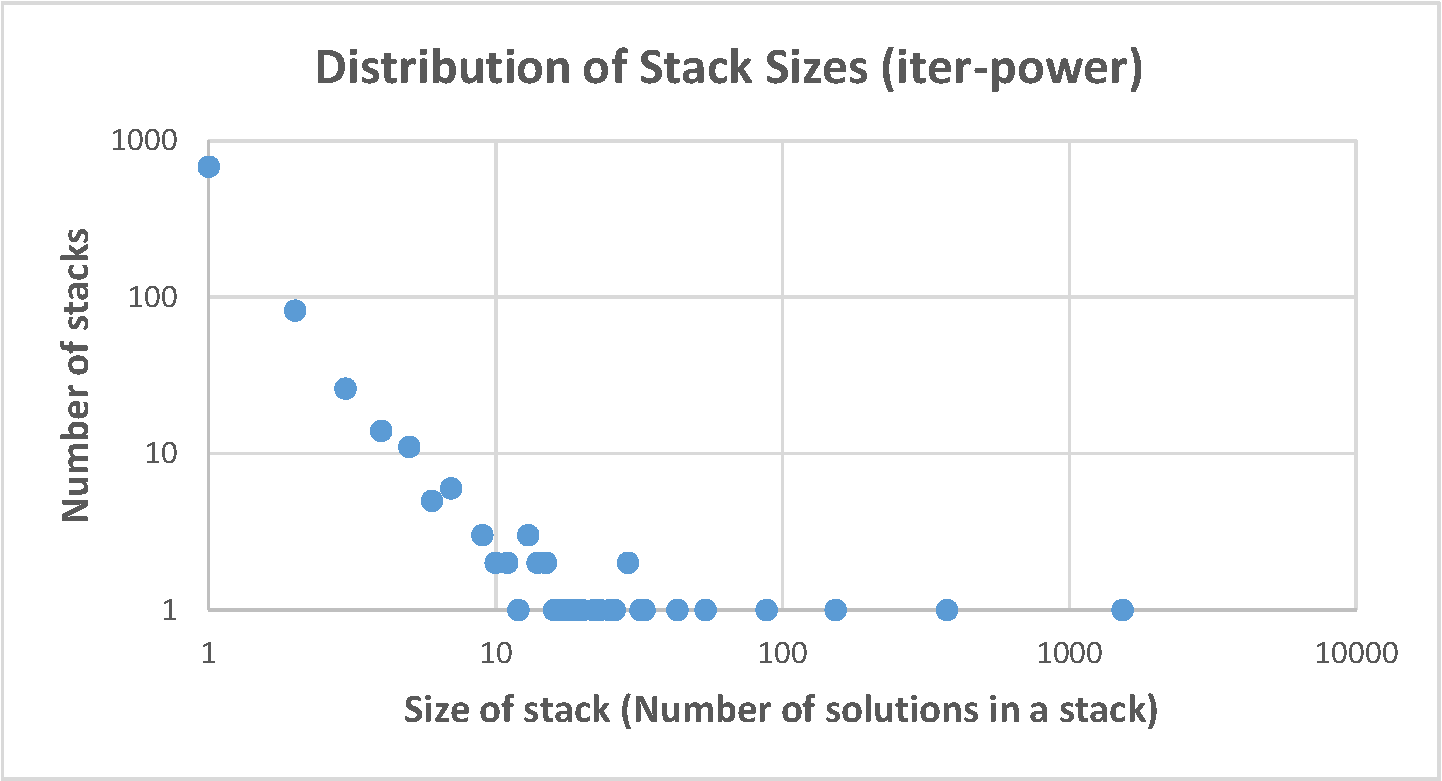
\includegraphics[scale=0.30]{Body/figures/overcode/stacksdistr-iter-power}
&
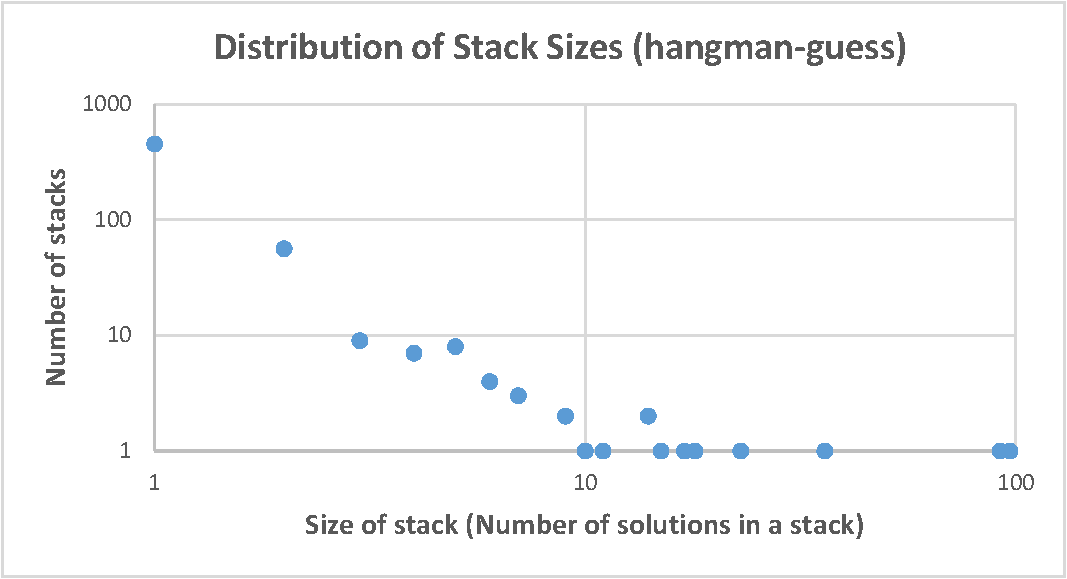
\includegraphics[scale=0.405]{Body/figures/overcode/stacksdistr-hangman}
\end{tabular}
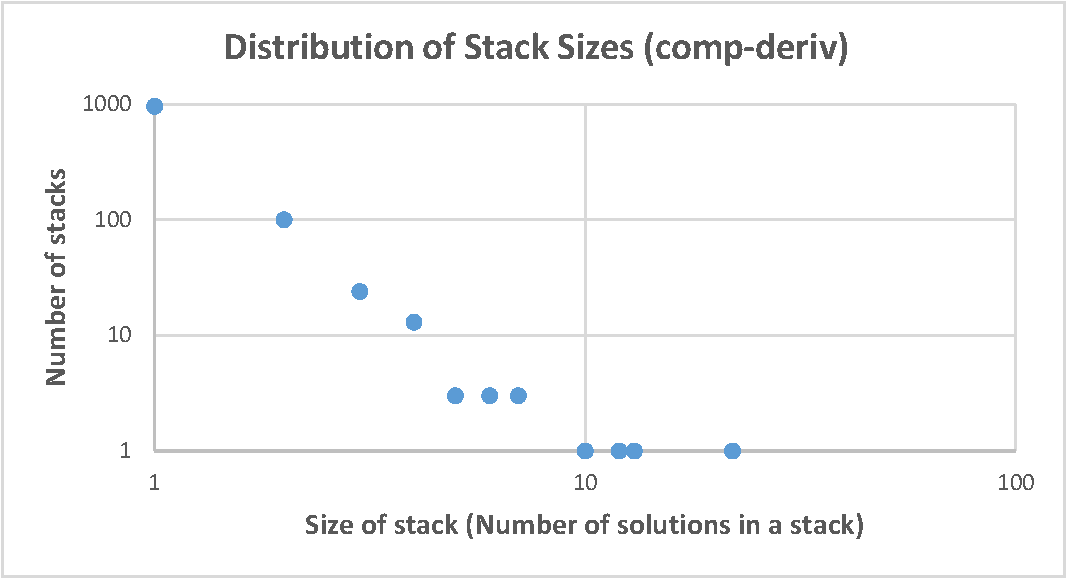
\includegraphics[scale=0.38]{Body/figures/overcode/stacksdistr-comp-deriv}
\caption{The distribution of sizes of the initial stacks generated by our algorithm for each problem\DIFdelbeginFL \DIFdelFL{. We can observe }\DIFdelendFL \DIFaddbeginFL \DIFaddFL{, showing }\DIFaddendFL a long tail distribution with a few large stacks and a lot of small stacks. Note that the two \DIFdelbeginFL \DIFdelFL{axis }\DIFdelendFL \DIFaddbeginFL \DIFaddFL{axes }\DIFaddendFL corresponding to the size of stacks and the number of stacks are in logarithmic scale.}
\label{stackdistribution}
\end{figure*}

\begin{figure}[h!]
\begin{tabular}{c}
\\
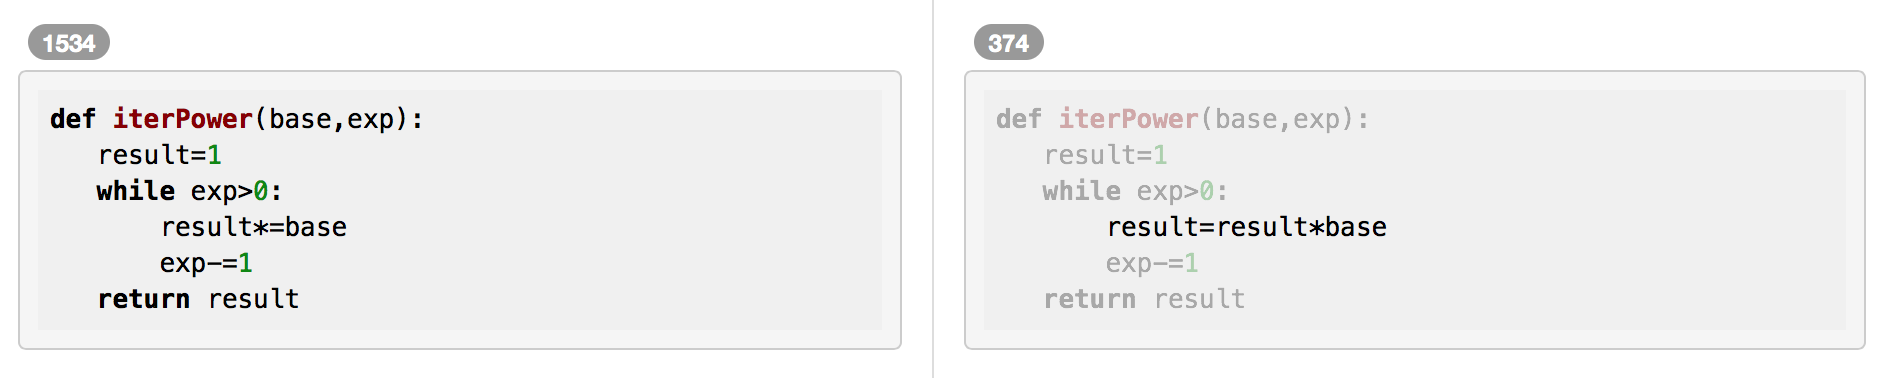
\includegraphics[scale=0.42]{Body/figures/overcode/iterpower-toptwo}
\\ (a) \\ \\
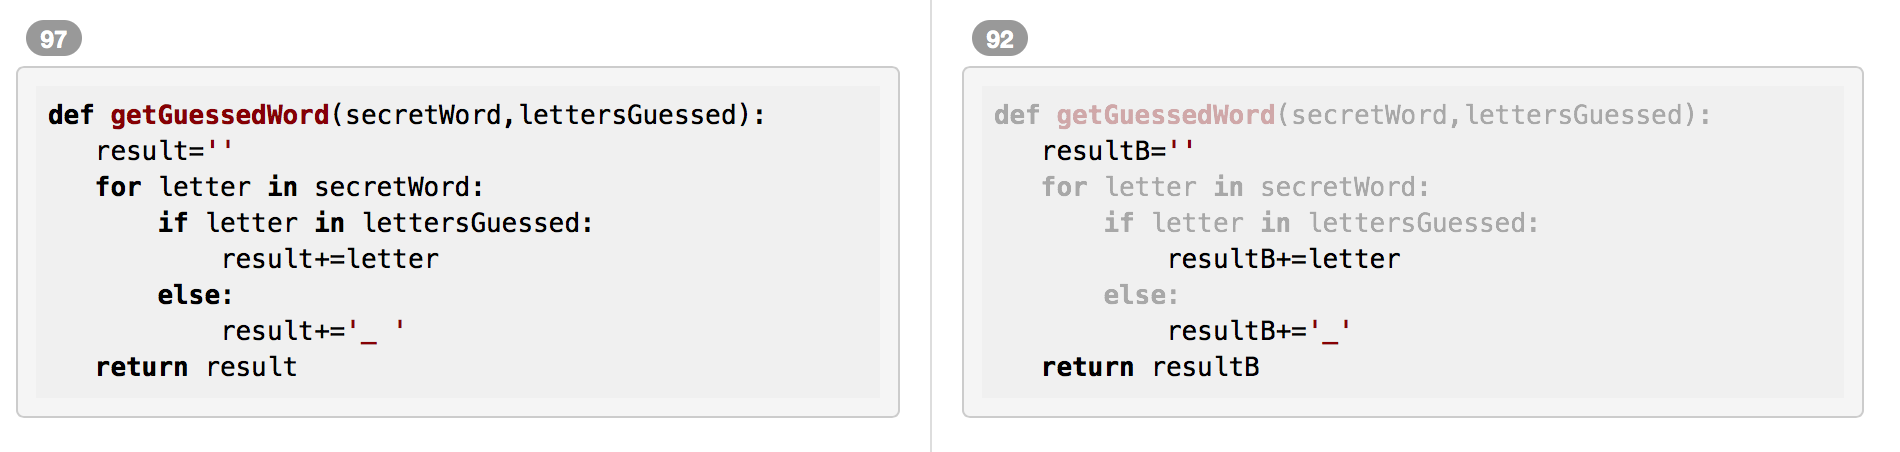
\includegraphics[scale=0.42]{Body/figures/overcode/hangman-toptwo}
\\ (b) \\ \\
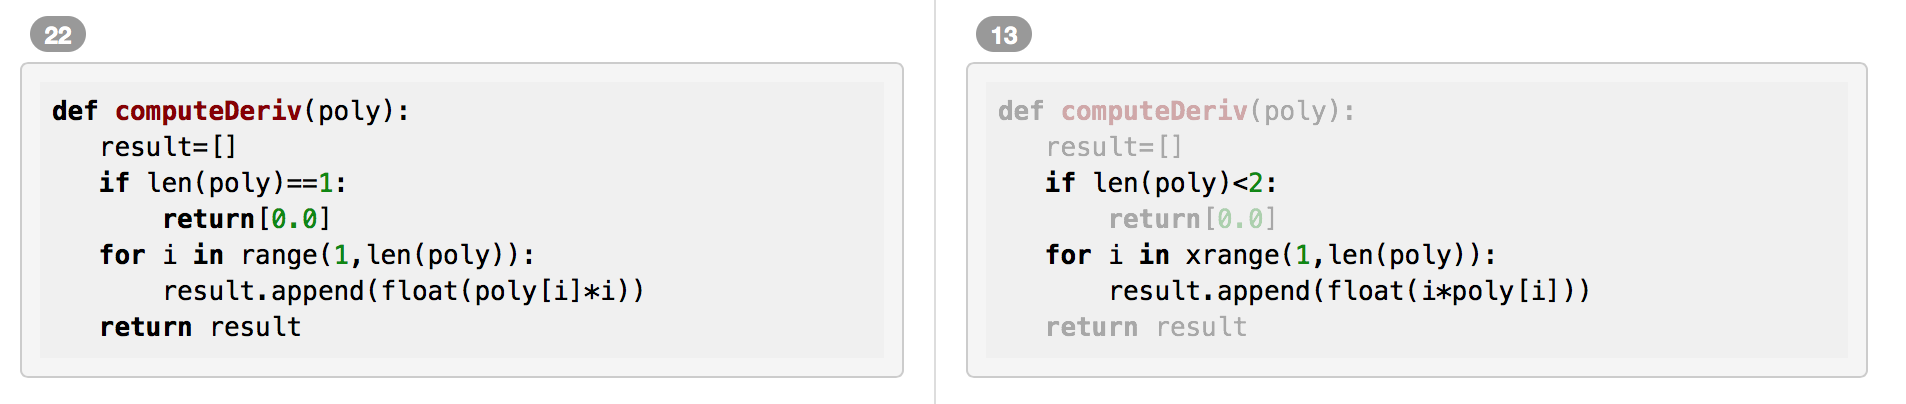
\includegraphics[scale=0.42]{Body/figures/overcode/compderiv-toptwo}
\\ (c) \\
\end{tabular}
\caption{The two largest stacks generated by the OverCode backend algorithm for the (a) \codevar{iterPower}, (b) \codevar{hangman}, and (c)  \codevar{compDeriv} problems.}
\label{toptwostacks}
\end{figure}

{\bf Common Variables} There exists a large variation among the variable names used by students to denote variables that compute the same set of values. The Variable Renaming step of the analysis renames these equivalent variables with the most frequently chosen variable name so that a teacher can easily recognize the role of variables in a given solution. The number of common variables found by the pipeline on the dataset problems is shown in Figure~\ref{backendevaluation} and some examples of these common variable names are shown in Figure~\ref{examplecommonvars}. Figure~\ref{examplecommonvars} also presents the number of times such a variable occurs across the solutions of a given problem, the corresponding variable sequence value on a given test input, and a subset of the original variable names used in the student solutions. 

\begin{figure}
\centering
\scriptsize
\begin{tabular} {|l|r|c|l|}
\hline
{\bf Common} & {\bf Occur} &  \multirow{3}{*}{\bf Sequence of Values} & \multirow{3}{*}{\bf Original Variable Names} \\
{\bf Variable} & {\bf -rence} & & \\
{\bf Name} & {\bf Count} & & \\
 \hline \hline
\multicolumn{4}{|c|}{}\\
\multicolumn{4}{|c|}{\bf iterPower}\\\hline
\codevar{result} & 3081 & [1,5.0,25.0,125.0] & \codevar{result}, \codevar{wynik}, \codevar{out}, \codevar{total}, \codevar{ans}, \codevar{acum}, \codevar{num}, \codevar{mult}, \codevar{output}, $\cdots$\\ \hline
\codevar{exp} & 2744 & [3,2,1,0] & \codevar{exp}, \codevar{iterator}, \codevar{app}, \codevar{ii}, \codevar{num}, \codevar{iterations}, \codevar{times}, \codevar{ctr}, \codevar{b}, $\cdots$\\ \hline
\codevar{exp} & 749 & [3] & \codevar{exp}, \codevar{count}, \codevar{temp}, \codevar{exp3}, \codevar{exp2}, \codevar{exp1}, \codevar{inexp}, \codevar{old\_exp}, $\cdots$\\ \hline
\codevar{i} & 266 & [0,1,2] & \codevar{i}, \codevar{a}, \codevar{count}, \codevar{c}, \codevar{b}, \codevar{iterValue}, \codevar{iter}, \codevar{n}, \codevar{y}, \codevar{inc}, \codevar{x},\codevar{times}, $\cdots$\\ \hline
\multicolumn{4}{|c|}{}\\
\multicolumn{4}{|c|}{\bf hangman}\\\hline
\codevar{letter} & 817 &  [`t',`i',`g',`e',`r'] & \codevar{letter}, \codevar{char}, \codevar{item}, \codevar{i}, \codevar{letS}, \codevar{ch}, \codevar{c}, \codevar{lett}, $\cdots$\\ \hline
\codevar{result} & 291 & [` ',`\_',`\_i',`\_i\_',`\_i\_e',`\_i\_e\_'] & \codevar{result}, \codevar{guessedWord}, \codevar{ans}, \codevar{str1}, \codevar{anss}, \codevar{guessed}, \codevar{string}, $\cdots$\\ \hline
\codevar{i} & 185 & [0,1,2,3,4] & \codevar{i}, \codevar{x}, \codevar{each}, \codevar{b}, \codevar{n}, \codevar{counter}, \codevar{idx}, \codevar{pos} $\cdots$\\ \hline
\codevar{found} & 76 & [0,1,0,1,0] & \codevar{found}, \codevar{n}, \codevar{letterGuessed}, \codevar{contains}, \codevar{k}, \codevar{checker}, \codevar{test}, $\cdots$\\ \hline
\multicolumn{4}{|c|}{}\\
\multicolumn{4}{|c|}{\bf compDeriv}\\ \hline
\codevar{result} & 1186 & [[],[0.0],$\cdots$,[0.0,35.0,9.0,4.0]] & \codevar{result}, \codevar{output}, \codevar{poly\_deriv}, \codevar{res}, \codevar{deriv}, \codevar{resultPoly}, $\cdots$\\ \hline
\codevar{i} & 284 &  [-13.39,0.0,17.5,3.0,1.0] & \codevar{i}, \codevar{each}, \codevar{a}, \codevar{elem}, \codevar{number}, \codevar{value}, \codevar{num}, $\cdots$\\ \hline
\codevar{i} & 261 & [0,1,2,3,4,5] & \codevar{i}, \codevar{power}, \codevar{index}, \codevar{cm}, \codevar{x}, \codevar{count}, \codevar{pwr}, \codevar{counter}, $\cdots$\\ \hline
\codevar{length} & 104 & [5] & \codevar{length}, \codevar{nmax}, \codevar{polyLen}, \codevar{lpoly}, \codevar{lenpoly}, \codevar{z}, \codevar{l}, \codevar{n}, $\cdots$\\ \hline

\end{tabular}
\caption{Some examples of common variables found by our analysis across the problems in the dataset. The table also shows the frequency of occurrence of these variables, the common sequence of values of these variables on a given test case, and a subset of the original variable names used by students.}
\label{examplecommonvars}
\end{figure}

{\bf Collisions in Variable Renaming} The number of Common/Common, Multiple Instances, and Unique/Common collisions discovered and resolved while performing variable renaming is shown in Figure~\ref{collisions}. A large majority of the collisions were Common/Common Collisions. For example, Figure~\ref{examplecommonvars} shows the common variable name \codevar{exp} for two different sequences of values $[3,2,1,0]$ and $[3]$ for the \codevar{iterPower} problem. Similarly, the common variable name \codevar{i} corresponds to sequences $[-13.9, 0.0, 17.5, 3.0, 1.0$ and $[0, 1, 2, 3, 4, 5]$ for the \codevar{compDeriv} problem. There were also a few Multiple Instances collisions and Unique/Common collisions found: 1.5\% for \codevar{iterPower}, 3\% for \codevar{compDeriv}, and 10\% for \codevar{hangman}.

\begin{figure}[htpb]
\centering
\begin{tabular}{|l|r|r|r|r|}
\hline
\multirow{2}{*}{\bf Problem} & {\bf Correct} & {\bf Common/Common} & {\bf Multiple Instances} & {\bf Unique/Common}\\
& {\bf Solutions} & {\bf Collisions } & {\bf Collisions} & {\bf Collisions}\\
\hline \hline
\codevar{iterPower} & 3875 & 1298 & 25 & 32 \\ \hline
\codevar{hangman} & 1118 & 672 & 62 & 49\\ \hline
\codevar{compDeriv} & 1433 & 928 & 21 & 23 \\ \hline
\end{tabular}
\caption{The number of common/common, multiple instances, and unique/common collisions discovered by our algorithm while renaming the variables to common names.}
\label{collisions}
\end{figure}

\DIFdelbegin %DIFDELCMD < \section{User Study 1: Writing a Class Forum Post}
%DIFDELCMD < %%%
\DIFdel{Our }\DIFdelend \DIFaddbegin \section{User Studies}

\DIFadd{The }\DIFaddend goal was to design a system that allows teachers to develop a better understanding of the variation in student solutions, and give feedback that is relevant to more \DIFdelbegin \DIFdel{students' solutions. We designed two user studies }\DIFdelend \DIFaddbegin \DIFadd{student solutions. Two user studies were designed }\DIFaddend to evaluate our progress in two ways: (1) user interface satisfaction and (2) how many solutions teachers could read and produce feedback on in a fixed amount of time. Reading and providing feedback to thousands of \DIFdelbegin \DIFdel{submissions }\DIFdelend \DIFaddbegin \DIFadd{solutions }\DIFaddend is an unrealistically difficult task for \DIFdelbegin \DIFdel{our }\DIFdelend \DIFaddbegin \DIFadd{the }\DIFaddend control condition, so instead of measuring time to finish the entire set of solutions, \DIFdelbegin \DIFdel{we sought to measure what our }\DIFdelend \DIFaddbegin \DIFadd{the experiment measures what }\DIFaddend subjects could accomplish in a fixed amount of time (15 minutes).

\DIFaddbegin \DIFadd{Together, these studies test four hypotheses:
} \begin{itemize} 
\item \textbf{\DIFadd{H1 Interface Satisfaction}} \DIFadd{Subjects will find OverCode easier to use, more helpful and less overwhelming for browsing thousands of solutions, compared to the baseline. 
}

\item {\bf \DIFadd{H2 Read coverage and speed}} \DIFadd{Subjects are able to read code that represents more student solutions at a higher rate using OverCode than with the baseline. 
}

\item {\bf \DIFadd{H3 Feedback coverage}} \DIFadd{Feedback produced when using OverCode is relevant to more student solutions than when feedback is produced using the baseline.
}

\item {\bf \DIFadd{H4 Perceived coverage}} \DIFadd{Subjects feel that they develop a better high-level view of students' understanding and misconceptions, and provide more relevant feedback using OverCode than with the baseline.
}

 \end{itemize} 

\subsection{User Study 1: Writing a Class Forum Post}

\DIFaddend The first study was a 12-person within-subjects evaluation of interface satisfaction when using OverCode for a realistic, relatively unstructured task. Using either OverCode or a baseline interface, subjects were asked to browse student solutions to the programming problems in our dataset and then write a class forum post on the good and bad ways students solved the problem. Through this study, \DIFdelbegin \DIFdel{we sought to test our first hypothesis :
}%DIFDELCMD < \begin{itemize}
 \begin{itemize} %DIFAUXCMD
%DIFDELCMD < \item %%%
\item%DIFAUXCMD
\textbf{\DIFdel{H1 Interface Satisfaction}}%DIFAUXCMD
\DIFdel{: Subjects will find OverCode easier to use, more helpful and less overwhelming for browsing thousands of solutions, compared to the baseline.
}
 \end{itemize} %DIFAUXCMD
%DIFDELCMD < \end{itemize}
%DIFDELCMD < %%%
\DIFdelend \DIFaddbegin \DIFadd{the first hypothesis is tested.
}\DIFaddend 

\DIFdelbegin %DIFDELCMD < \subsection{OverCode and Baseline Interfaces}
%DIFDELCMD < %%%
\DIFdelend \DIFaddbegin \subsubsection{OverCode and Baseline Interfaces}
\DIFaddend 

\DIFdelbegin \DIFdel{We designed two interfaces }\DIFdelend \DIFaddbegin \DIFadd{Two interfaces were designed}\DIFaddend , referred to here as OverCode and the baseline. The OverCode interface and backend are described in detail in Section \ref{overcode}. The baseline interface was a single webpage with all student solutions concatenated in a random order into a flat list (Figure \ref{iterPowerEdXControl}, left). \DIFdelbegin \DIFdel{We chose this design to emulate }\DIFdelend \DIFaddbegin \DIFadd{This design emulates }\DIFaddend existing methods of reviewing solutions, and \DIFaddbegin \DIFadd{aims }\DIFaddend to draw out differences between browsing stacked and unstacked solutions. This is analogous to the ``flat'' interface chosen as a baseline for Basu et al.'s interface for grading clusters of short answers~\cite{basuDivideAndConquer}. Basu et al.'s assumption, that existing options for reviewing solutions are limited to going through solutions one-by-one, is backed by our pilot studies and interviews with teaching staff, and our own grading experiences. In fact, in edX programming MOOCs, teachers are not even provided with an interface for viewing all solutions at once\DIFdelbegin \DIFdel{; they }\DIFdelend \DIFaddbegin \DIFadd{. They }\DIFaddend can only look at one student \DIFdelbegin \DIFdel{'s }\DIFdelend solution at a time. If the solutions can be downloaded locally, some teachers may use \DIFdelbegin \DIFdel{within-file search functions like the command line utility }\DIFdelend \DIFaddbegin \DIFadd{a search tool like }\DIFaddend \codevar{grep}. Our baseline allows \DIFdelbegin \DIFdel{that }\DIFdelend \DIFaddbegin \DIFadd{for search }\DIFaddend too, through the in-browser \DIFdelbegin \DIFdel{find }\DIFdelend \DIFaddbegin \texttt{\DIFadd{Find}} \DIFaddend command. 

In the baseline, solutions appeared visually similar to those in the OverCode interface (boxed, syntax-highlighted code), but the solutions were \DIFdelbegin \emph{\DIFdel{raw}}%DIFAUXCMD
\DIFdelend \DIFaddbegin \DIFadd{raw}\DIFaddend , in the sense that they were not normalized for whitespace or variable naming differences. As in the OverCode condition, subjects were able to use standard web-browser features, such as the within-page \DIFdelbegin \emph{\DIFdel{find}} %DIFAUXCMD
\DIFdelend \DIFaddbegin \texttt{\DIFadd{Find}} \DIFaddend action.


\begin{figure}[h!]
\centering
\begin{tabular}{cc}
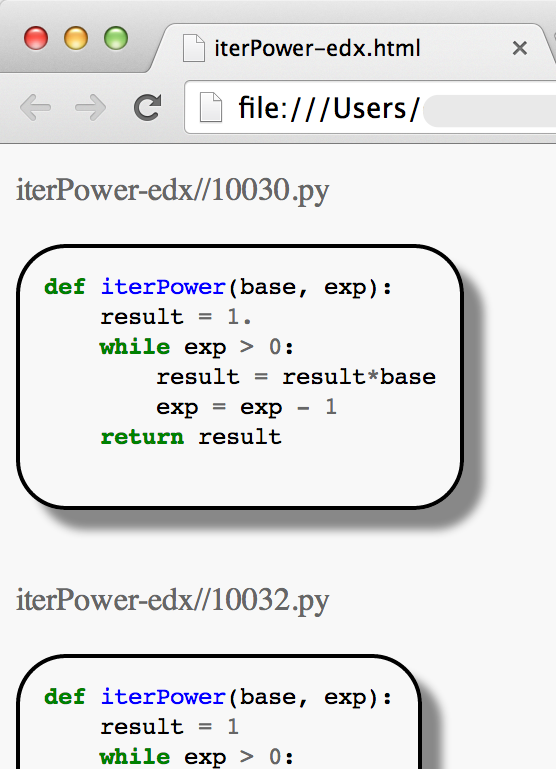
\includegraphics[scale=0.5]{Body/figures/overcode/iterPowerEdXControlStudy1.png} &
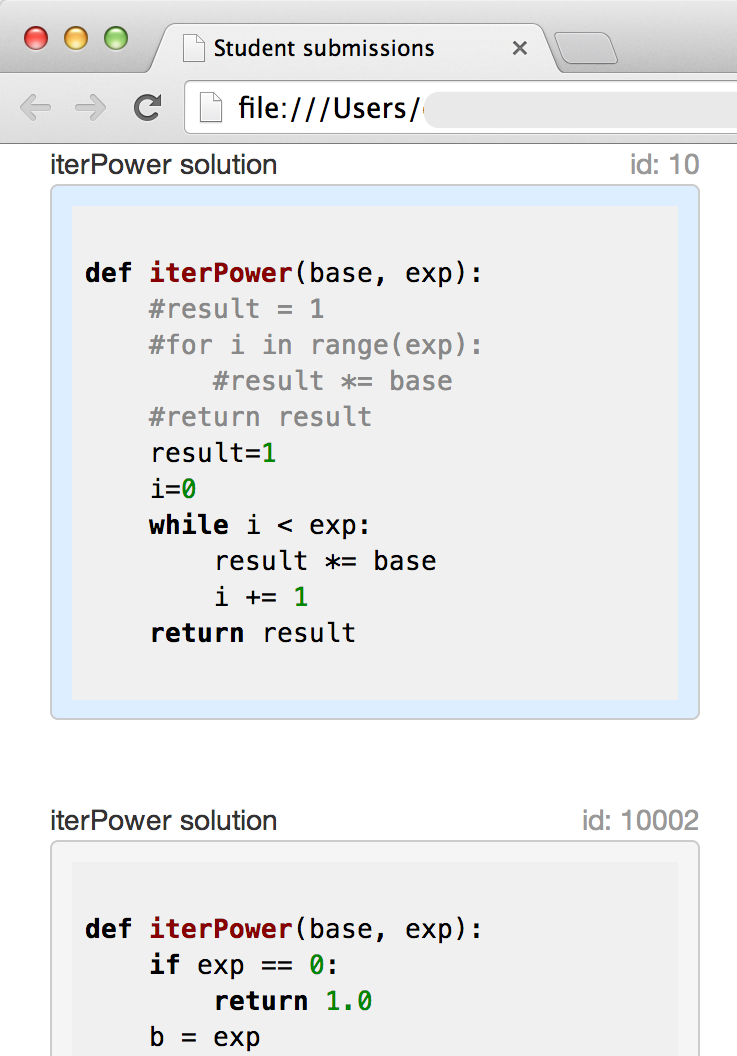
\includegraphics[scale=0.37]{Body/figures/overcode/iterPowerEdXControlStudy2.png} \\
\end{tabular}
\caption{\DIFdelbeginFL \DIFdelFL{The }\DIFdelendFL \DIFaddbeginFL \DIFaddFL{Screenshots of the }\DIFaddendFL baseline interface\DIFdelbeginFL \DIFdelFL{used in }\DIFdelendFL \DIFaddbeginFL \DIFaddFL{. The appearance did not change significantly between }\DIFaddendFL the Forum Post study \DIFdelbeginFL \DIFdelFL{(}\DIFdelendFL \DIFaddbeginFL \DIFaddFL{control interface, shown on the }\DIFaddendFL left\DIFdelbeginFL \DIFdelFL{) }\DIFdelendFL \DIFaddbeginFL \DIFaddFL{, }\DIFaddendFL and the Coverage study \DIFdelbeginFL \DIFdelFL{(}\DIFdelendFL \DIFaddbeginFL \DIFaddFL{control interface, shown on the }\DIFaddendFL right\DIFdelbeginFL \DIFdelFL{)}\DIFdelendFL . \DIFaddbeginFL \DIFaddFL{Functionality did not change at all.}\DIFaddendFL }
\label{iterPowerEdXControl}
\end{figure}
\DIFdelbegin %DIFDELCMD < \subsection{Participants}
%DIFDELCMD < %%%
\DIFdelend 

\DIFdelbegin \DIFdel{We recruited participants }\DIFdelend \DIFaddbegin \subsubsection{Participants}

\DIFadd{Participants were recruited }\DIFaddend by reaching out to past and present programming course staff \DIFaddbegin \DIFadd{at our university}\DIFaddend , and advertising on an \DIFdelbegin \DIFdel{academic computer science research lab's }\DIFdelend \DIFaddbegin \DIFadd{MIT CSAIL }\DIFaddend email list. These individuals were qualified to participate in our study because they met at least one of the following requirements: (1) \DIFdelbegin \DIFdel{were current teaching staff of }\DIFdelend \DIFaddbegin \DIFadd{have taught }\DIFaddend a computer science course (2) \DIFdelbegin \DIFdel{had }\DIFdelend \DIFaddbegin \DIFadd{have }\DIFaddend graded Python code before, or (3) \DIFdelbegin \DIFdel{had }\DIFdelend \DIFaddbegin \DIFadd{have }\DIFaddend significant Python programming experience, making them potential future teaching staff. \DIFaddbegin \DIFadd{Subjects were offered \$20 to participate. 
}\DIFaddend 

Information about the subjects' backgrounds was collected during recruitment and again at the beginning of their \DIFdelbegin \DIFdel{one hour }\DIFdelend \DIFaddbegin \DIFadd{one-hour }\DIFaddend in-lab user study session. 12 people (7 male) participated, with a mean age of 23.5 ($\sigma = 3.8$). Subjects had a mean 4 years of Python programming experience ($\sigma = 1.8$), and $75\%$ of participants had graded student solutions written in Python before. Half of the participants were graduate students \DIFdelbegin \DIFdel{, and }\DIFdelend \DIFaddbegin \DIFadd{and the }\DIFaddend other half were undergraduates.

\DIFdelbegin %DIFDELCMD < \subsection{Apparatus}
%DIFDELCMD < %%%
\DIFdelend \DIFaddbegin \subsubsection{Apparatus}
\DIFaddend 

\DIFdelbegin \DIFdel{Each subject was given \$20 to participate in a 60 minute session with an experimenter, in an on-campus academic lab conference room. They }\DIFdelend \DIFaddbegin \DIFadd{Subjects }\DIFaddend used laptops running MacOS and Linux with screen sizes ranging from 12.5 to 15.6 inches, and viewed the OverCode and baseline interfaces in either Safari or Chrome. Data was recorded with Google Docs and Google Forms filled out by participants.
\DIFdelbegin %DIFDELCMD < \subsection{Conditions}
%DIFDELCMD < %%%
\DIFdelend 

\DIFaddbegin \subsubsection{Conditions}

\DIFaddend Subjects performed the main task of browsing solutions and writing a class forum post twice, once in each interface condition, focusing on one of the three problems in our dataset (Section \ref{dataset}) each time. For each participant, the third remaining problem was used during training, to reduce learning effects when performing the two main tasks. The pairing and ordering of interface and problem conditions were fully counterbalanced, resulting in 12 total conditions. The twelve participants were randomly assigned to one of the 12 conditions, such that all conditions were tested.

\DIFdelbegin %DIFDELCMD < \subsection{Procedure}
%DIFDELCMD < %%%
\DIFdelend \DIFaddbegin \subsubsection{Procedure}
\DIFaddend 

\DIFdelbegin %DIFDELCMD < \subsubsection{Prompt}
%DIFDELCMD < %%%
\DIFdelend \DIFaddbegin {\bf \DIFadd{Prompt}} \DIFaddend The experimenter began by reading the following prompt, to give the participant context for the tasks they would be performing:

\begin{quote}

We want to help TAs [teaching assistants] give feedback to students in programming classes at scale. For each of three problems, we have a large set of students' submissions ($> 1000$). 

All the submissions are correct, in terms of input and output behavior. We're going to ask you to browse the submissions and produce feedback for students in the class. You'll do this primarily in the form of a class forum post.
\end{quote}

To make the task more concrete, participants were given an example\footnote{Our example was drawn from the blog ``Practice Python: 30-minute weekly Python exercises for beginners,'' posted on Thursday, April 24, 2014, and titled ``SOLUTION Exercise 11: Check Primality and Functions.'' (\url{http://practicepython.blogspot.com})} of a class forum post that used examples taken from student solutions to explain different strategies for solving a Python problem. They were also given print-outs of the prompts for each of the three problems in our dataset, to reference when looking at solutions.
\DIFdelbegin %DIFDELCMD < \subsubsection{Training}
%DIFDELCMD < %%%
\DIFdelend 

\DIFaddbegin {\bf \DIFadd{Training}} \DIFaddend Given the subjects' extensive experience with web-browsers, training for the baseline interface was minimal. Prior to using the OverCode interface, subjects watched a 3-4 minute long training video demonstrating the features of OverCode, and were given an opportunity to become familiar with the interface and ask questions. The training session focused on the problem that would not be used in the main tasks, in order to avoid learning effects.

\DIFdelbegin %DIFDELCMD < \subsubsection{Tasks}
%DIFDELCMD < %%%
\DIFdelend \DIFaddbegin {\bf \DIFadd{Tasks}} \DIFaddend Subjects then performed the main tasks twice, once in each interface, focusing on a different programming problem each time. They were given a fixed amount of time to both read solutions and provide feedback, so \DIFdelbegin \DIFdel{we did not measure }\DIFdelend task completion times \DIFaddbegin \DIFadd{were not measured}\DIFaddend , but instead the quality of their experience in providing feedback to students at scale.

 \begin{itemize} 
\item {\it Feedback for Students} (15 minutes) Subjects were asked to write a class forum post on the good and bad ways students solved the problem. The \DIFdelbegin \DIFdel{fifteen minute }\DIFdelend \DIFaddbegin \DIFadd{15-minute }\DIFaddend period included both browsing and writing time, as subjects were free to paste in code examples and write comments as they browsed the solutions.

\item {\it Autograder Bugs} (2 min) Although the datasets of student solutions were marked as correct by an autograder, there may be holes in the autograder \DIFdelbegin \DIFdel{'s }\DIFdelend test cases. Some solutions may deviate from the problem prompt, and therefore be considered incorrect by teachers, e.g., recursive solutions to \codevar{iterPower} when its prompt explicitly calls for an iterative solution. As a secondary task, \DIFdelbegin \DIFdel{we asked subjects }\DIFdelend \DIFaddbegin \DIFadd{subjects were asked }\DIFaddend to write down any bugs in the autograder they came across while browsing solutions. This was often performed concurrently with the primary task by the subject.
 \end{itemize} 
\DIFdelbegin %DIFDELCMD < \subsubsection{Surveys}
%DIFDELCMD < %%%
\DIFdelend \DIFaddbegin {\bf \DIFadd{Surveys}} \DIFaddend Subjects filled out a post-interface condition survey about their experience using the interface. This was a short-answer survey, where they wrote about what they liked, what they did not like, and what they would like to see in a future version of the interface. At the end of the study, subjects rated agreement (on a 7-point Likert scale) with statements about their satisfaction with each interface.

\DIFdelbegin %DIFDELCMD < \subsection{Results}
%DIFDELCMD < %%%
\textbf{\DIFdel{H1}} %DIFAUXCMD
\DIFdel{is supported by ratings from the post-study survey (see }\DIFdelend \DIFaddbegin \subsubsection{Results}
\DIFaddend Figure~\ref{study1Likert} \DIFdelbegin \DIFdel{). Statistical significance was computed using the Wilcoxon Signed Rank test, pairing users' ratings of each interface}\DIFdelend \DIFaddbegin \DIFadd{shows that, compared to the control interface, subjects find OverCode less overwhelming, easier to use, and more helpful for getting a sense of students' understanding}\DIFaddend . After using both interfaces to view thousands of solutions, subjects found OverCode easier to use (\DIFdelbegin \DIFdel{W=52, Z=2.41, p<0.05, r=0.70}\DIFdelend \DIFaddbegin \DIFadd{$W=52, Z=2.41, p<0.05, r=0.70$}\DIFaddend ) and less overwhelming (\DIFdelbegin \DIFdel{W = 0, Z = -2.86, p < 0.005, r = 0.83}\DIFdelend \DIFaddbegin \DIFadd{$W=0, Z=-2.86, p<0.005, r=0.83$}\DIFaddend ) than the baseline interface. Finally, participants felt that OverCode ``helped me get a better sense of my students' understanding'' than the baseline did (\DIFdelbegin \DIFdel{W = 66, Z = 3.04, p < 0.001, r = 0.88). }\DIFdelend \DIFaddbegin \DIFadd{$W=66, Z=3.04, p<0.001, r=0.88$). These differences are statistically significant, as computed by the Wilcoxon Signed Rank test with pairing users' ratings of each interface. This supports }\textbf{\DIFadd{H1}}\DIFadd{.
}\DIFaddend 

\begin{figure}
\centering
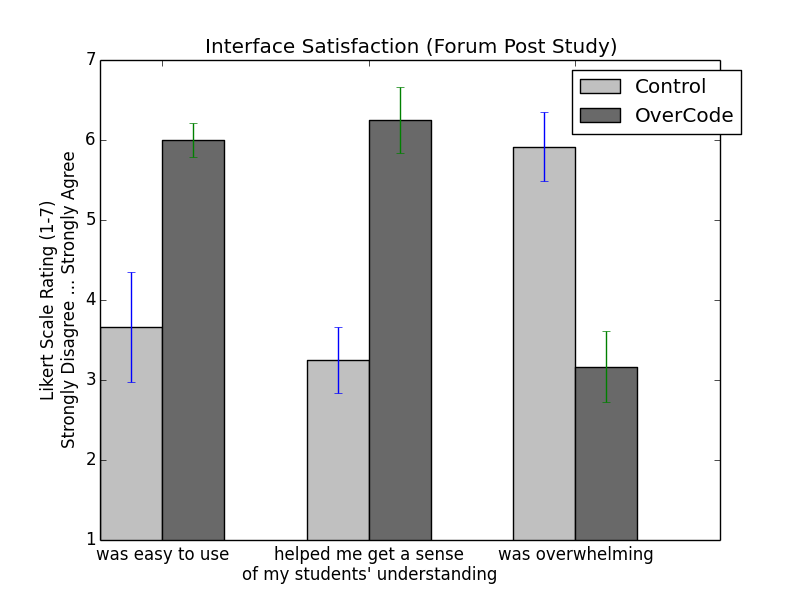
\includegraphics[scale=0.5]{Body/figures/overcode/study1Likert.png}
\caption{{\bf H1: Interface satisfaction} Mean Likert scale ratings (with standard error) for OverCode and baseline interfaces, after subjects used both to perform the forum post writing task.}
\label{study1Likert}
\end{figure}


From the surveys conducted after subjects completed each interface condition, \DIFdelbegin \DIFdel{we found that }\DIFdelend subjects found stacking and the ability to rewrite code to be useful and enjoyable features of OverCode:
 \begin{itemize} 
\item \DIFaddbegin {\it \DIFaddend Stacking is an awesome feature. Rewrite tool is fantastic. Done feature is very rewarding--feels much less overwhelming. "Lines that appear in x submissions" also awesome.\DIFaddbegin }
\DIFaddend 

\item \DIFaddbegin {\it \DIFaddend Really liked the clever approach for variable normalization. Also liked the fact that stacks showed numbers, so I'd know I'm focusing on the highest-impact submissions. Impressed by the rewrite ability... it cut down on work so much!\DIFaddbegin }
\DIFaddend 

\item \DIFaddbegin {\it \DIFaddend I liked having solutions collapsed (not having to deal with variable names, etc), and having rules to allow me to collapse even further. This made it easy to see the \DIFdelbegin \DIFdel{"plurality" }\DIFdelend \DIFaddbegin \DIFadd{``plurality'' }\DIFaddend of solutions right away; I spent most of the time looking at the solutions that only had a few instances.\DIFaddbegin }
\DIFaddend  \end{itemize} 

When asked for suggestions, participants gave many suggestions on stacks, filtering, and rewrite rules, such as:
 \begin{itemize} 
\begin{comment}
\item Augment the stacks with a representation of the output of the code in that stack, since the autograder can consider more than one particular output ``correct.'' 
\end{comment}
\item Enable the \DIFdelbegin \DIFdel{user }\DIFdelend \DIFaddbegin \DIFadd{teacher }\DIFaddend to change the main stack that is being compared against the others.
\item Suggest possible rewrite rules, based on what the \DIFdelbegin \DIFdel{user }\DIFdelend \DIFaddbegin \DIFadd{teacher }\DIFaddend has already written, and will not affect the answers on the test case.
\item Create a filter that shows all stacks that do {\DIFdelbegin %DIFDELCMD < \emph %%%
\DIFdelend \DIFaddbegin \it \DIFaddend not} have a particular statement.
 \end{itemize} 

For both the OverCode and baseline interfaces, the feedback generated about \codevar{iterPower}, \codevar{hangman}, and \codevar{compDeriv} solutions fell into several common themes. One kind of feedback suggested new language features, such as using \codevar{*=} or the keyword \codevar{in}. Another theme identified inefficient, redundant, and convoluted control flow, such as repeated statements and unnecessary statements and variables. It was not always clear what the misconception was, though, as one participant wrote, \textit{``The double iterator solution surely shows some lack of grasp of power of for loop, or range, or something.''} \DIFdelbegin \DIFdel{Participants' }\DIFdelend \DIFaddbegin \DIFadd{Participant }\DIFaddend feedback included comments on the relative goodness of different correct solutions in the dataset. This was a more holistic look at \DIFdelbegin \DIFdel{students' }\DIFdelend \DIFaddbegin \DIFadd{student }\DIFaddend solutions as they varied along the dimensions of conciseness, clarity, and efficiency previously described.

Study participants found both noteworthy correct solutions and solutions they considered incorrect, despite passing the autograder. One participant learned a new Python function, \codevar{enumerate}, while looking at a solution that used it. The participant wrote, \textit{``Cool, but uncalled for. I had to look it up :]. Use, but with comment.''} Participants also found recursive \codevar{iterPower} and \codevar{hangman} solutions, which they found noteworthy. For what should have been an iterative \codevar{iterPower} function, the fact that this recursive solution was considered correct by the \DIFdelbegin \DIFdel{unit-test-based }\DIFdelend autograder was considered an autograder bug by some participants. Using the built-in Python exponentiation operator \codevar{**} was also considered correct by the autograder, even though it subverted the point of the assignment. It was also noted as an autograder bug by some participants who found it.
\DIFdelbegin %DIFDELCMD < \section{User Study 2: Coverage}
%DIFDELCMD < %%%
\DIFdelend 

\DIFdelbegin \DIFdel{We designed a }\DIFdelend \DIFaddbegin \subsection{User Study 2: Coverage}

\DIFadd{A }\DIFaddend second 12-person study \DIFaddbegin \DIFadd{was designed}\DIFaddend , similar in structure to the forum post study, but focused on measuring the coverage achieved by subjects in a fixed amount of time (15 minutes) when browsing and producing feedback on a large number of student solutions. The second study's task was more constrained than the first: instead of writing a freeform post, subjects were asked to identify the five most frequent strategies used by students and rate their confidence that these strategies \DIFdelbegin \DIFdel{occurred frequently }\DIFdelend \DIFaddbegin \DIFadd{were frequently used }\DIFaddend in the student solutions. These changes to the task \DIFdelbegin \DIFdel{, as well as modifications to the OverCode and baseline interfaces, }\DIFdelend enabled us to measure coverage in terms of solutions read, the relevance of written feedback and the subject's perceived coverage. \DIFdelbegin \DIFdel{We sought to test the following hypotheses:
}%DIFDELCMD < 

%DIFDELCMD < \begin{itemize}
%DIFDELCMD < \item {\bf %%%
\DIFdelend \DIFaddbegin \DIFadd{In this study, the rest of the hypotheses, i.e., }\DIFaddend H2\DIFdelbegin \DIFdel{Read coverage and speed}%DIFDELCMD < } %%%
\DIFdel{Subjects are able to read code that represents more student solutions at a higher rate using OverCode than with the baseline. 
}%DIFDELCMD < 

%DIFDELCMD < \item {\bf %%%
\DIFdelend \DIFaddbegin \DIFadd{, }\DIFaddend H3\DIFdelbegin \DIFdel{Feedback coverage}%DIFDELCMD < } %%%
\DIFdel{Feedback produced when using OverCode is relevant to more students' solutions than when feedback is produced using the baseline}\DIFdelend \DIFaddbegin \DIFadd{, and H4, are tested}\DIFaddend .

\DIFdelbegin %DIFDELCMD < \item {\bf %%%
\DIFdel{H4 Perceived coverage}%DIFDELCMD < } %%%
\DIFdel{Subjects feel that they develop a better high-level view of students' understanding and misconceptions, and provide more relevant feedback using OverCode than with the baseline}\DIFdelend \DIFaddbegin \DIFadd{Prior to running the second study, both the OverCode and baseline interfaces were slightly modified. Figure \ref{iterPowerEdXControl} shows the baseline changes that reduce the differences between the rendering of solutions in the baseline and OverCode interfaces. The OverCode interface was changed to show identifiers next to every stack and solutions so that subjects could provide it when asked}\DIFaddend .

\DIFdelbegin %DIFDELCMD < \end{itemize}
%DIFDELCMD < %%%
\DIFdelend \DIFaddbegin \subsubsection{Participants, Apparatus, Conditions}
\DIFaddend 

\DIFdelbegin %DIFDELCMD < \subsection{Participants, Apparatus, Conditions}
%DIFDELCMD < 

%DIFDELCMD < %%%
\DIFdelend The coverage study shared the same methods for recruiting participants, apparatus and conditions as the forum post study. 12 new participants (11 male) participated in the second study (mean age = 25.4, $\sigma = 6.9$). Across those 12 participants, the mean years of Python programming experience was 4.9 ($\sigma = 3.0$) and 9 of them had previously graded code (5 had graded Python code). There were 5 graduate students, 6 undergraduates, and 1 independent computer software professional.


\DIFdelbegin %DIFDELCMD < \subsection{Interface Modifications}
%DIFDELCMD < %%%
\DIFdel{Prior to the second study, both the OverCode and baseline interfaces were slightly modified (see differences in Figure \ref{iterPowerEdXControl}) in order to enable measurements of read coverage, feedback coverage and perceived coverage.
}%DIFDELCMD < \begin{itemize}
 \begin{itemize} %DIFAUXCMD
%DIFDELCMD < \item %%%
\item%DIFAUXCMD
\DIFdel{Clicking on stacks or solutions caused the box of code to be outlined in blue. This enabled the subject to mark them as }\emph{\DIFdel{read}}%DIFAUXCMD
\footnote{\DIFdel{In the OverCode condition, this replaced the }\emph{\DIFdel{done}} %DIFAUXCMD
\DIFdel{checkboxes, in that clicking stacks caused the progress bar to update.}} %DIFAUXCMD
\addtocounter{footnote}{-1}%DIFAUXCMD
\DIFdel{and enabled us to measure read coverage.
}%DIFDELCMD < \item %%%
\item%DIFAUXCMD
\DIFdel{Stacks and solutions were all marked with an identifier, which subjects were asked to include with each piece of feedback they produced. This enabled us to more easily compute feedback coverage, which will be explained further in Section~\ref{coverageResults}.
}%DIFDELCMD < \item %%%
\item%DIFAUXCMD
\DIFdel{All interface interactions were logged in the browser console, allowing us to track both the subject's read coverage over time, as well as their usage of other features, such as the creation of rewrite rules to merge stacks.
}%DIFDELCMD < \item %%%
\item%DIFAUXCMD
\DIFdel{Where it differed slightly before, we changed the styling of code in the baseline condition to exactly match the code in the OverCode condition.
}
 \end{itemize} %DIFAUXCMD
%DIFDELCMD < \end{itemize}
%DIFDELCMD < \subsection{Procedure}
%DIFDELCMD < \subsubsection{Prompt}
%DIFDELCMD < %%%
\DIFdelend \DIFaddbegin \subsubsection{Procedure}
{\bf \DIFadd{Prompt}} \DIFaddend In the coverage study, the prompt was similar to the one used in the forum post study, explaining that the subjects would be tackling the problem of producing feedback for students at scale. The language was modified to shift the focus towards finding frequent strategies used by students, rather than any example of good or bad code used by a student.\DIFaddbegin \todo{find prompt and put it in here}
\DIFaddend 

\DIFdelbegin %DIFDELCMD < \subsubsection{Training}
%DIFDELCMD < %%%
\DIFdelend \DIFaddbegin {\bf \DIFadd{Training}} \DIFaddend As before, subjects were shown a training video and given time to practice using OverCode \DIFdelbegin \DIFdel{'s }\DIFdelend features prior to their trial in the OverCode condition.

\DIFdelbegin %DIFDELCMD < \subsubsection{Task}
%DIFDELCMD < %%%
\DIFdelend \DIFaddbegin {\bf \DIFadd{Task}} \DIFaddend The coverage study \DIFdelbegin \DIFdel{'s }\DIFdelend task consisted of a more constrained feedback task. Given 15 minutes with either the OverCode or baseline interface, subjects were asked to fill out a table, identifying the \DIFdelbegin \DIFdel{5 }\DIFdelend \DIFaddbegin \DIFadd{five }\DIFaddend most frequent strategies used by students to solve the problem. For each strategy they identified, they were asked to fill in the following fields in the table:
 \begin{itemize} 
\item A code example taken from the solution or stack.
\item The identifier of the solution or stack.
\item A short (\DIFdelbegin \DIFdel{1 }\DIFdelend \DIFaddbegin \DIFadd{one }\DIFaddend sentence) annotation of what was good or bad about the strategy.
\item Their confidence, on a scale of 1-7, that the strategy frequently occurred in the student solutions.
 \end{itemize} 
Importantly, subjects were also asked to mark solutions or stacks as \emph{read} by clicking on them after they had \DIFdelbegin \DIFdel{`processed ' }\DIFdelend \DIFaddbegin \DIFadd{processed }\DIFaddend them, even if they \DIFdelbegin \DIFdel{weren't }\DIFdelend \DIFaddbegin \DIFadd{were not }\DIFaddend choosing them as representative strategies. Combined with interaction logging done by the system, this enabled us to measure read coverage.

\DIFdelbegin %DIFDELCMD < \begin{comment}
%DIFDELCMD < \begin{figure}[h!]
%DIFDELCMD < 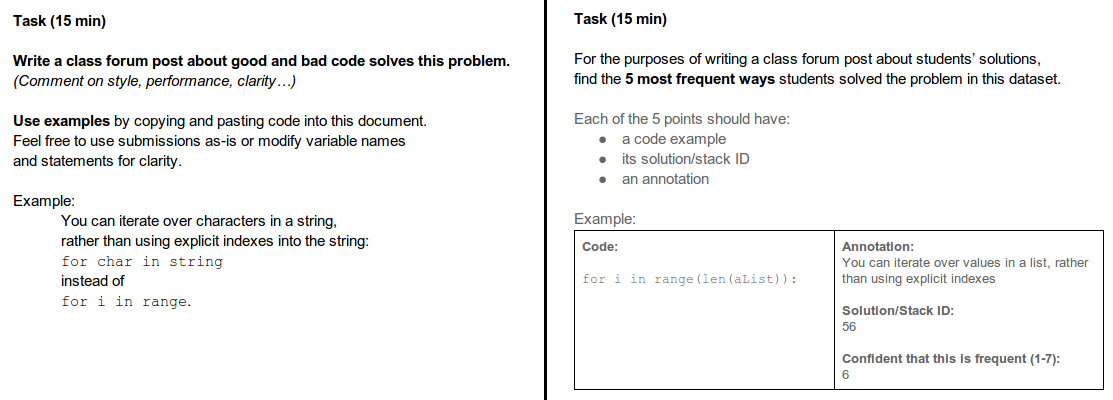
\includegraphics[width=0.6\paperwidth]{figures/study-prompts.png}
%DIFDELCMD < %%%
%DIFDELCMD < \caption{%
{%DIFAUXCMD
\DIFdelFL{Prompts given to subjects in Study 1 (left) and Study 2 (right).}}
%DIFAUXCMD
%DIFDELCMD < %DIFDELCMD < \label{studyPrompts}%%%
%DIFDELCMD < \end{figure}
%DIFDELCMD < \end{comment}
%DIFDELCMD < \subsubsection{Surveys} 
%DIFDELCMD < 

%DIFDELCMD < %%%
\DIFdelend \DIFaddbegin {\bf \DIFadd{Surveys}} \DIFaddend Although we measured interface satisfaction for a realistic task in the forum post study, we also measured interface satisfaction through surveys for this more constrained, coverage-focused task. Subjects filled out a post-interface condition survey in which they rated agreement (on a 7-point Likert scale) with positive and negative adjectives about their experience using the interface, and reflected on task difficulty. At the end of the study, subjects were asked to rate their agreement with statements about the usefulness of specific features of both the OverCode and baseline interfaces, and responded to the same interface satisfaction 7-point Likert scale statements used in the first study.

\DIFdelbegin %DIFDELCMD < \subsection{Results} %%%
\DIFdelend \DIFaddbegin \subsubsection{Results} \DIFaddend \label{coverageResults}
\begin{figure*}[b!]
\begin{tabular}{c | c}
\begin{minipage}{.5\linewidth}
\centering
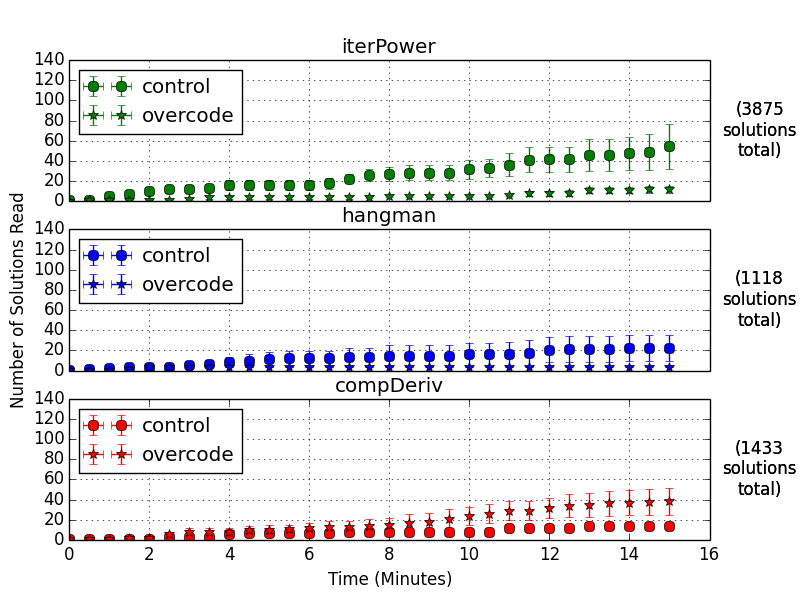
\includegraphics[width=\linewidth]{Body/figures/overcode/prettyReadCoverage.png}
\end{minipage}
&
\begin{minipage}{.5\linewidth}
\centering
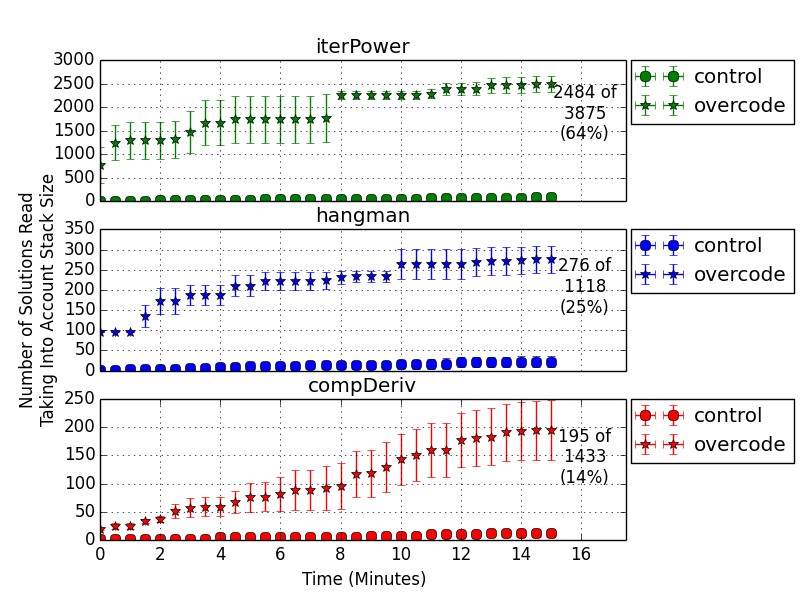
\includegraphics[width=\linewidth]{Body/figures/overcode/prettyPercentCoverage.png}
\end{minipage}
\\
(a) & (b)
\end{tabular}
\caption{In (a), we plot the mean number of \DIFdelbeginFL \DIFdelFL{cleaned }\DIFdelendFL \DIFaddbeginFL \DIFaddFL{platonic }\DIFaddendFL solutions \DIFdelbeginFL \DIFdelFL{representing stacks }\DIFdelendFL read in OverCode over time versus the number of raw solutions read in the baseline interface over time while performing the \DIFdelbeginFL \DIFdelFL{15 minute long }\DIFdelendFL \DIFaddbeginFL \DIFaddFL{15-minute }\DIFaddendFL Coverage Study task. In (b), we replace the mean number of \DIFdelbeginFL \DIFdelFL{cleaned }\DIFdelendFL \DIFaddbeginFL \DIFaddFL{platonic }\DIFaddendFL solutions with the mean number of solutions\DIFdelbeginFL \DIFdelFL{(}\DIFdelendFL \DIFaddbeginFL \DIFaddFL{, i.e., }\DIFaddendFL the \DIFaddbeginFL \DIFaddFL{stack }\DIFaddendFL size\DIFdelbeginFL \DIFdelFL{of the stacks) }\DIFdelendFL \DIFaddbeginFL \DIFaddFL{, }\DIFaddendFL they represent. These are shown for each of the three problems in \DIFdelbeginFL \DIFdelFL{our }\DIFdelendFL \DIFaddbeginFL \DIFaddFL{the }\DIFaddendFL dataset.}
\label{readCoverage}
\end{figure*}
\DIFdelbegin %DIFDELCMD < \subsubsection{H2: Read coverage and speed}
%DIFDELCMD < %%%
\DIFdel{This hypothesis is supported by our measurements of read coverage from this study. For each problem, subjects were able to view more cleaned and stacked solutions by the end of the 15 minute long main task using OverCode than raw solutions when using the baseline interface }\DIFdelend \DIFaddbegin 

{\bf \DIFadd{H2: Read coverage and speed}} \DIFadd{Figure \ref{readCoverage} shows that subjects reading platonic }\texttt{\DIFadd{iterPower}}\DIFadd{, }\texttt{\DIFadd{hangman}}\DIFadd{, and }\texttt{\DIFadd{compDeriv}} \DIFadd{solutions in the OverCode interface covered the equivalent of 64\%, 25\%, and 14\% of all student solutions to those problems }\DIFaddend (Mann--Whitney U = 16, n1 = n2 = 4, p<0.05). \DIFdelbegin \DIFdel{Figure \ref{readCoverage} shows the mean number of solutions read over time for each interface and each problem in our dataset.The curves show that subjects were able to read code that represented more raw solutionsat a higher rate due to the stacking of similar solutions}\DIFdelend \DIFaddbegin \DIFadd{Subjects read through more raw solutions than platonic solutions to the simplest problems, i.e., }\texttt{\DIFadd{iterPower}} \DIFadd{and }\texttt{\DIFadd{hangman}}\DIFadd{, but when problem difficulty increased, i.e., }\texttt{\DIFadd{compDeriv}}\DIFadd{, subjects read through OverCode's platonic solutions faster than raw solutions. This supports the H2 hypothesis}\DIFaddend .

\DIFdelbegin %DIFDELCMD < \subsubsection{H3: Feedback coverage}
%DIFDELCMD < %%%
\DIFdelend %DIF > This hypothesis is supported by our measurements of read coverage from this study. For each problem, subjects were able to view more normalized and stacked solutions by the end of the 15-minute-long main task using OverCode than raw solutions when using the baseline interface (Mann--Whitney U = 16, n1 = n2 = 4, p<0.05). Figure \ref{readCoverage} shows the mean number of solutions read over time for each interface and each problem in our dataset. The curves show that subjects were able to read code that represented more raw solutions at a higher rate due to the stacking of similar solutions.

\DIFdelbegin %DIFDELCMD < \begin{figure}[b!]
%DIFDELCMD < 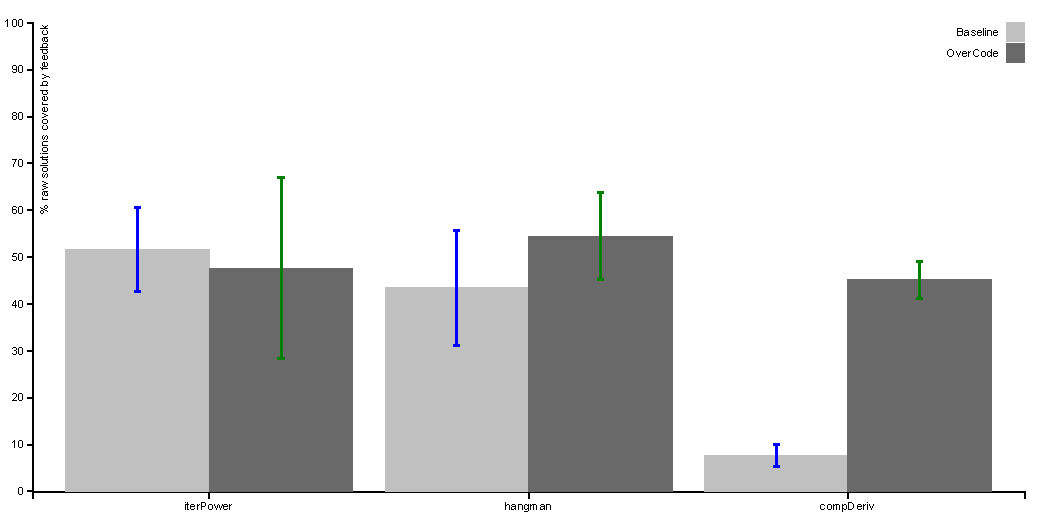
\includegraphics[width=0.6\paperwidth]{Body/figures/overcode/feedbackCoverage.pdf}
%DIFDELCMD < %%%
%DIFDELCMD < \caption{%
{%DIFAUXCMD
\DIFdelFL{Mean feedback coverage (percentage of raw solutions) per trial during the coverage study for each problem, in the OverCode and baseline interfaces.}}
%DIFAUXCMD
%DIFDELCMD < %DIFDELCMD < \label{aveCoveragePerPost}%%%
%DIFDELCMD < \end{figure}
%DIFDELCMD < 

%DIFDELCMD < %%%
\DIFdelend \DIFaddbegin {\bf \DIFadd{H3: Feedback coverage}} \DIFaddend Each subject reported on the \DIFdelbegin \DIFdel{5 }\DIFdelend \DIFaddbegin \DIFadd{five }\DIFaddend most frequent strategies in a set of solutions, by copying both a code example and the identifier of the solution (baseline) or stack (OverCode) that it came from. We define \emph{feedback coverage} as the number of students for which the quoted code is relevant, in the sense that they wrote the same lines of code, ignoring differences in whitespace or variable names. We computed the coverage for each example using the following process:
 \begin{itemize} 
\item Reduce the quoted code down to only the lines referred to in the annotation. Often, the subject's annotation would focus on a specific feature of the quoted code, which sometimes had additional lines that were unrelated to the subject's feedback. For example, comments about iterating over a range function, while also quoting the contents of the for loop. This step meant we would be calculating the coverage of a more general (smaller) set of lines.

\item Find the source stack that the quoted code comes from. This is trivial in the OverCode condition, where the stack ID is included in the subject's post. In the baseline, we used the solution ID included in the subject's post to find the stack that it was merged into by the backend pipeline.

\item Find the \DIFdelbegin \DIFdel{cleaned }\DIFdelend \DIFaddbegin \DIFadd{normalized }\DIFaddend version of each quoted line. The quoted lines of code may be raw code if they come from the baseline condition. By comparing the quoted code with the \DIFdelbegin \DIFdel{cleaned }\DIFdelend \DIFaddbegin \DIFadd{normalized }\DIFaddend code of its source stack, we found the \DIFdelbegin \DIFdel{cleaned }\DIFdelend \DIFaddbegin \DIFadd{normalized }\DIFaddend version of each line, with variable names and whitespace normalized.

\item Find the raw solutions that include the set of \DIFdelbegin \DIFdel{cleaned }\DIFdelend \DIFaddbegin \DIFadd{normalized }\DIFaddend lines, using a map from stacks to raw solutions provided by the backend pipeline.
 \end{itemize} 

\DIFaddbegin \begin{figure}[b!]
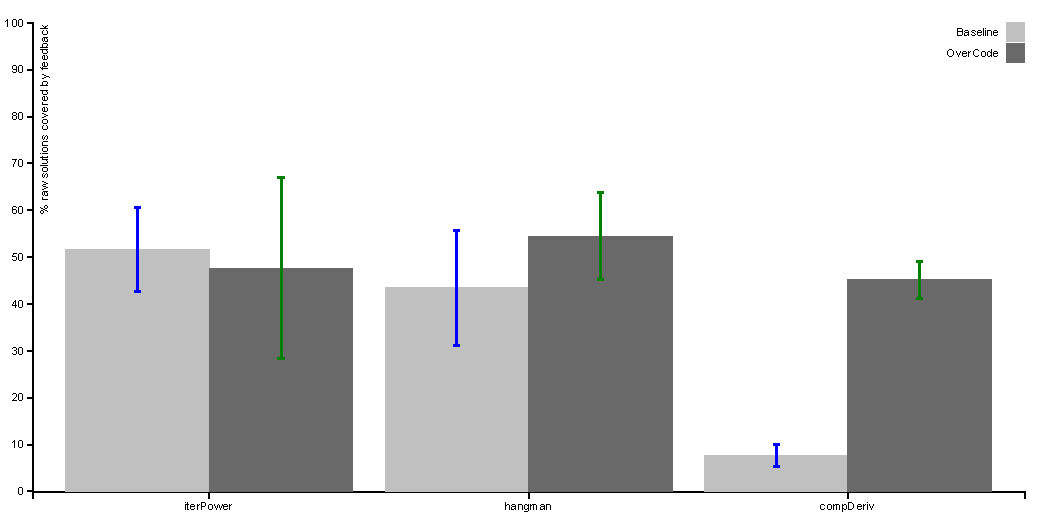
\includegraphics[width=0.6\paperwidth]{Body/figures/overcode/feedbackCoverage.pdf}
\caption{\DIFaddFL{Mean feedback coverage, i.e., the percentage of raw solutions covered, per trial during the coverage study for each problem, in the OverCode and baseline interfaces.}}
\label{aveCoveragePerPost}
\end{figure}
%DIF > \todo{DNHT: what are the error bars?}

\DIFaddend Figure \ref{aveCoveragePerPost} shows the mean coverage of a set of feedback produced by a single subject, across problems and interface conditions. The feedback coverage is shown as the mean percentage of raw solutions for which the feedback was relevant. When giving feedback on the \codevar{iterPower} and \codevar{hangman} problems, there was not a statistically significant difference in the feedback coverage between interface conditions. However, on \codevar{compDeriv}, the problem with the most complex solutions, subjects using OverCode were able to achieve significantly more coverage of student solutions than when using the baseline interface (Mann--Whitney U = 0, n1 = n2 = 4, p< 0.05).

\DIFdelbegin %DIFDELCMD < \subsubsection{H4: Perceived coverage}
%DIFDELCMD < 

%DIFDELCMD < %%%
\DIFdelend \begin{figure*}[t!]
\begin{tabular}{c | c}
\begin{minipage}{.5\linewidth}
\centering
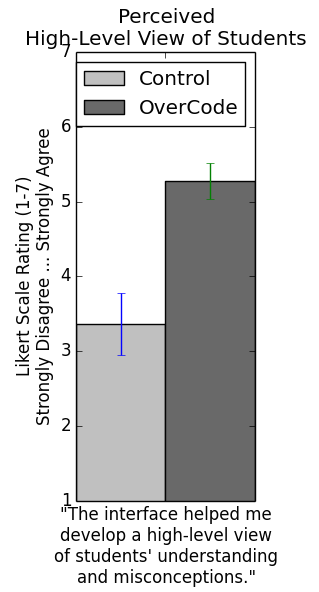
\includegraphics[scale=0.5]{Body/figures/overcode/highLevelViewStudy2.png}
\end{minipage}
&
\begin{minipage}{.5\linewidth}
\centering
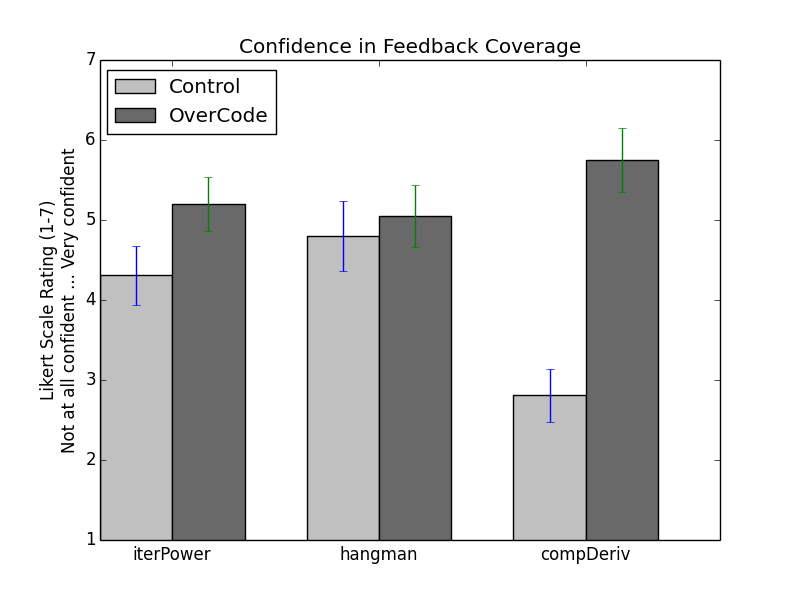
\includegraphics[width=\linewidth]{Body/figures/overcode/coverageConfidence.png}
\end{minipage}
\\
(a) & (b)
\end{tabular}
\caption{\DIFaddbeginFL \DIFaddFL{Mean rating with standard error for }\DIFaddendFL (a) \DIFdelbeginFL \DIFdelFL{Post-condition }\DIFdelendFL \DIFaddbeginFL \DIFaddFL{post-condition }\DIFaddendFL perception of coverage (excluding one participant) and (b) \DIFdelbeginFL \DIFdelFL{Confidence }\DIFdelendFL \DIFaddbeginFL \DIFaddFL{confidence }\DIFaddendFL ratings that identified strategies \DIFaddbeginFL \DIFaddFL{were }\DIFaddendFL frequently \DIFdelbeginFL \DIFdelFL{occurred }\DIFdelendFL \DIFaddbeginFL \DIFaddFL{used }\DIFaddendFL (1-7 scale).}
\label{perceivedCoverage}
\end{figure*}

\DIFdelbegin \DIFdel{Immediately after }\DIFdelend \DIFaddbegin {\bf \DIFadd{H4: Perceived coverage}} \DIFadd{After }\DIFaddend using each interface, we asked participants how strongly they agreed with the statement `This interface helped me develop a high-level view of students' understanding and misconceptions,' which quotes the first part of our third hypothesis. Participants agreed with this statement after using OverCode significantly more than when using the baseline interface (\DIFdelbegin \DIFdel{W=63, Z=2.70,p<0.01,r=0.81}\DIFdelend \DIFaddbegin \DIFadd{$W=63, Z=2.70, p<0.01, r=0.81$}\DIFaddend ). Statistical significance was computed using the Wilcoxon Signed Rank test, pairing users' ratings of each interface. The analysis was done on 11 participants' data, as one participant's data was lost. The mean rating \DIFdelbegin \DIFdel{(}\DIFdelend with standard error \DIFdelbegin \DIFdel{) }\DIFdelend for the responses is shown in Figure~\ref{perceivedCoverage}(a). 

For each strategy identified by subjects, we asked them to rate their confidence, on a scale of 1-7, that the strategy was frequently used by students in the dataset. Mean confidence ratings on a per-problem basis are shown in Figure \ref{perceivedCoverage}(b). We found that for \codevar{compDeriv}, subjects using OverCode were significantly more confident that their annotations were relevant to many students, compared to the baseline (Mann--Whitney \DIFdelbegin \DIFdel{U = 260.5, n1 = 18 n2 = 16, p< 0.0001}\DIFdelend \DIFaddbegin \DIFadd{$U=260.5, n_{1}=18, n_{2}=16, p<0.0001$}\DIFaddend ).

\DIFdelbegin %DIFDELCMD < \subsubsection{H1: Interface satisfaction}
%DIFDELCMD < 

%DIFDELCMD < %%%
\DIFdel{Interface satisfaction}\DIFdelend \DIFaddbegin {\bf \DIFadd{H1: Interface satisfaction}} \DIFadd{Interface satisfaction }\DIFaddend was measured through multiple surveys, (1) immediately after using each interface and (2) after using both interfaces. Statistical significance was computed using the Wilcoxon Signed Rank test, pairing users' ratings of each interface. 

Immediately after finishing the assigned tasks with an interface, participants rated their agreement with statements about the appropriateness of various adjectives to describe the interface they just used, on a 7-point Likert scale. While participants found the baseline to be significantly more simple (\DIFdelbegin \DIFdel{W=2.5, Z=-2.60,p<0.01,r=0.78}\DIFdelend \DIFaddbegin \DIFadd{$W=2.5, Z=-2.60, p<0.01, r=0.78$}\DIFaddend ), they found OverCode to be significantly more flexible (\DIFdelbegin \DIFdel{W=45, Z=2.84, p<0.005, r=0.86}\DIFdelend \DIFaddbegin \DIFadd{$W=45, Z=2.84, p<0.005, r=0.86$}\DIFaddend ), less tedious (\DIFdelbegin \DIFdel{W=3.5, Z=-2.41, p<0.05, r=0.73}\DIFdelend \DIFaddbegin \DIFadd{$W=3.5, Z=-2.41, p<0.05, r=0.73$}\DIFaddend ), more interesting (\DIFdelbegin \DIFdel{W=66, Z=2.96, p<0.001, r=0.89}\DIFdelend \DIFaddbegin \DIFadd{$W=66, Z=2.96, p<0.001, r=0.89$}\DIFaddend ), and more enjoyable (\DIFdelbegin \DIFdel{W=45, Z=2.83, p<0.005, r=0.85}\DIFdelend \DIFaddbegin \DIFadd{$W=45, Z=2.83, p<0.005, r=0.85$}\DIFaddend ). The analysis was done on 11 participants' data, as one participant's data was lost. The mean ratings (with standard error) for the responses \DIFdelbegin \DIFdel{is }\DIFdelend \DIFaddbegin \DIFadd{are }\DIFaddend shown in Figure~\ref{studyLikert1_onPop2}. 

After the completion of the Coverage Study, participants were asked again to rate their agreement with statements about each interface on a 7-point Likert scale. After using both interfaces to view thousands of solutions, there were no significant differences between how overwhelming or easy to use each interface was. However, participants did feel that OverCode ``helped me get a sense of my students' understanding'' more than the baseline (\DIFdelbegin \DIFdel{W=62.5, Z=-2.69, p<0.01, r=0.78}\DIFdelend \DIFaddbegin \DIFadd{$W=62.5, Z=-2.69, p<0.01, r=0.78$}\DIFaddend ). The mean ratings (with standard error) for the responses \DIFdelbegin \DIFdel{is }\DIFdelend \DIFaddbegin \DIFadd{are }\DIFaddend shown in Figure~\ref{studyLikert1_onPop2}.

\begin{figure}
\centering
\begin{tabular}{c c}
\begin{minipage}{.6\linewidth}
\centering
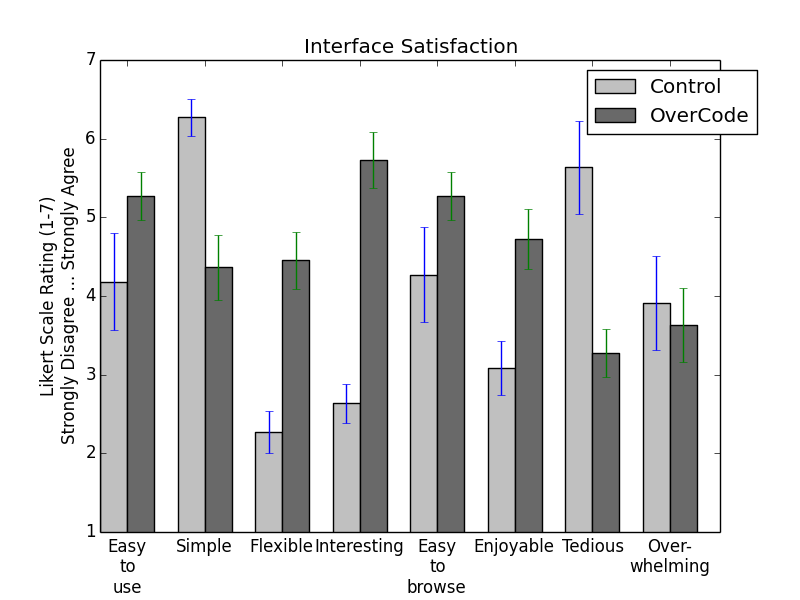
\includegraphics[scale=0.35]{Body/figures/overcode/study2Likert.png}
\end{minipage}
&
\begin{minipage}{.4\linewidth}
\centering
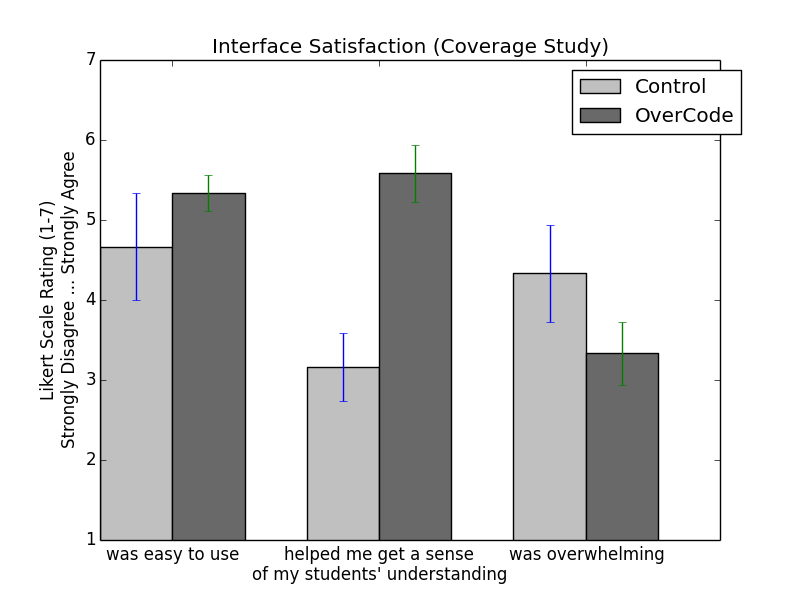
\includegraphics[scale=0.30]{Body/figures/overcode/study1Likert_onPop2.png}
\end{minipage}
\\
(a) & (b)
\end{tabular}
\caption{{\bf H1: Interface satisfaction} Mean Likert scale ratings (with standard error) for  OverCode and baseline, (a) immediately after using the interface for the Coverage Study task, and (b) after using both interfaces.}
\label{studyLikert1_onPop2}
\end{figure}

\DIFdelbegin %DIFDELCMD < \subsubsection{Usage and Usefulness of Interface Features}
%DIFDELCMD < 

%DIFDELCMD < %%%
\DIFdelend \DIFaddbegin {\bf \DIFadd{Usage and Usefulness of Interface Features}} \DIFaddend In the second part of the post-study survey, participants rated their agreement with statements about the helpfulness of various interface features on a 7-point Likert scale. There were only two features to ask about in the baseline interface (in-browser find and viewing raw solutions), which were mixed in with statements about features in the OverCode interface. The OverCode feature of stacking equivalent solutions was found more helpful than the baseline \DIFdelbegin \DIFdel{'s }\DIFdelend features of in-browser find (\DIFdelbegin \DIFdel{W=41, Z=2.07, p<0.05, r=0.60}\DIFdelend \DIFaddbegin \DIFadd{$W=41, Z=2.07, p<0.05, r=0.60$}\DIFaddend ) and viewing raw \DIFdelbegin \DIFdel{students' }\DIFdelend \DIFaddbegin \DIFadd{student }\DIFaddend solutions, comments included (\DIFdelbegin \DIFdel{W=45, Z=2.87,p<0.005,r=0.83}\DIFdelend \DIFaddbegin \DIFadd{$W=45, Z=2.87, p<0.005, r=0.83$}\DIFaddend ). The OverCode feature of variable renaming and previewing rewrite rules were also both found significantly more helpful than seeing \DIFdelbegin \DIFdel{students' raw code (W=65.5,Z=2.09,p<0.05,r=0.61 and W=56.5, Z=2.14, p<0.05, r=0.62, }\DIFdelend \DIFaddbegin \DIFadd{raw student code ($W=65.5, Z=2.09, p<0.05, r=0.61$ and $W=56.5, Z=2.14, p<0.05, r=0.62$, }\DIFaddend respectively). The mean ratings for the features are shown in Figure~\ref{featureHelpfulness}.

\begin{figure}
\centering
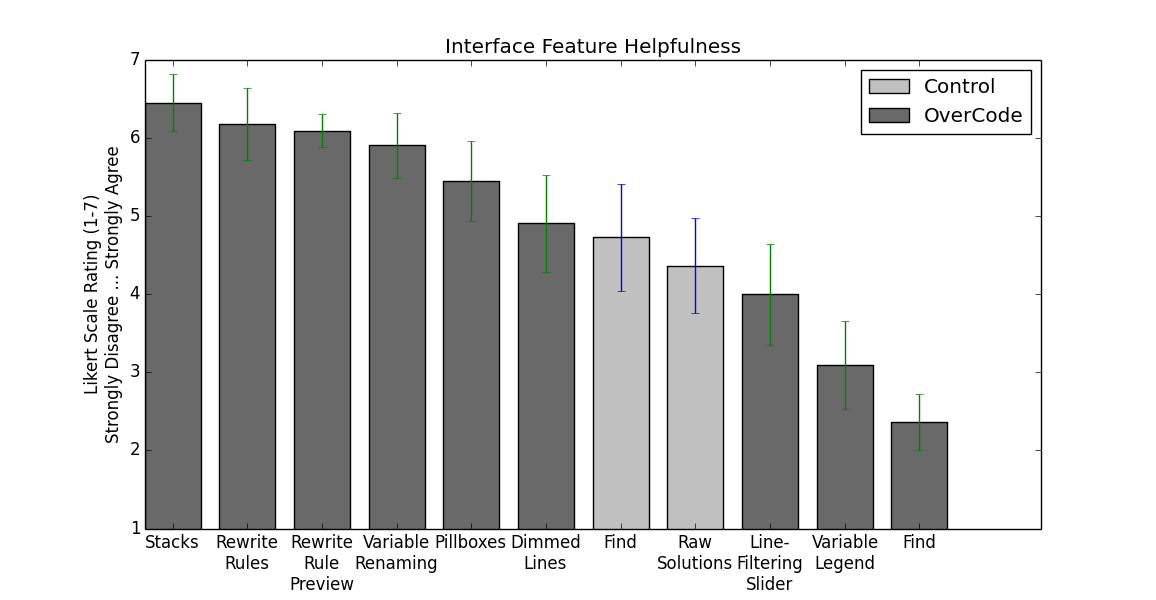
\includegraphics[scale=0.5]{Body/figures/overcode/featureHelpfulness.png}
\caption{Mean Likert scale ratings (with standard error) for the usefulness of features of OverCode and baseline. \DIFdelbeginFL \DIFdelFL{``}\DIFdelendFL \DIFaddbeginFL {\it \DIFaddendFL Find\DIFdelbeginFL \DIFdelFL{'' is }\DIFdelendFL \DIFaddbeginFL } \DIFaddFL{refers to }\DIFaddendFL the \DIFaddbeginFL \DIFaddFL{find function within the }\DIFaddendFL web browser\DIFdelbeginFL \DIFdelFL{'s built-in find, which }\DIFdelendFL \DIFaddbeginFL \DIFaddFL{. }{\it \DIFaddFL{Find}} \DIFaddendFL appears twice \DIFaddbeginFL \DIFaddFL{in this figure }\DIFaddendFL because users rated its usefulness for each condition.}
\label{featureHelpfulness}
\end{figure}

In addition to logging \codevar{read} events, we also recorded usage of interface features, such as creating rewrite rules and filtering stacks. A common usage strategy was to read through the stacks linearly and mark them as \codevar{read}, starting with the largest reference stack, then rewrite trivial variations in expressions to merge smaller \DIFdelbegin \DIFdel{behaviorally-equivalent }\DIFdelend \DIFaddbegin \DIFadd{behaviorally equivalent }\DIFaddend stacks into the largest stack. Stack filtering (Figure~\ref{linefilter}) was sometimes used to review solutions that contained a particularly conspicuous line\DIFdelbegin \DIFdel{(}\DIFdelend \DIFaddbegin \DIFadd{, }\DIFaddend e.g.\DIFaddbegin \DIFadd{, }\DIFaddend a recursive call to solve \codevar{iterPower} \DIFdelbegin \DIFdel{, }\DIFdelend or an extremely long expression\DIFdelbegin \DIFdel{)}\DIFdelend . The filter \DIFdelbegin \DIFdel{'s }\DIFdelend \DIFaddbegin \DIFadd{panel }\DIFaddend frequency slider (Figure~\ref{linefilter}a) and the variable legend (Figure~\ref{afterrewrite}b) were scarcely used.

All subjects wrote at least two rewrite rules, often causing stacks to merge that only differed in some trivial way, like reordering operands in multiplication statements\DIFdelbegin \DIFdel{(}\DIFdelend \DIFaddbegin \DIFadd{, }\DIFaddend e.g.\DIFaddbegin \DIFadd{, }\DIFaddend \codevar{result = result*base} vs. \codevar{result = base*result}\DIFdelbegin \DIFdel{)}\DIFdelend . Some rewrite rules merged Python expressions that behaved similarly but differed in their verbosity\DIFdelbegin \DIFdel{(}\DIFdelend \DIFaddbegin \DIFadd{, }\DIFaddend e.g.\DIFaddbegin \DIFadd{, }\DIFaddend \codevar{for i in range(0, exp)} vs. \codevar{for i in range(exp)}\DIFdelbegin \DIFdel{) - variations that might }\DIFdelend \DIFaddbegin \DIFadd{. These variations may }\DIFaddend be considered noteworthy or trivial by different teachers.
\DIFaddbegin 

\DIFaddend \section{Discussion}

Our three-part evaluation of \DIFdelbegin \DIFdel{OverCode's }\DIFdelend \DIFaddbegin \DIFadd{the OverCode }\DIFaddend backend and user interface demonstrates its usability and usefulness in a realistic teaching scenario. Given that we focused on the first three weeks of an introductory Python programming course, our evaluation is limited to single functions, whose most common solutions were less than ten lines long. Some of these functions were recursive, while most were iterative. Variables were generally limited to booleans, integers, strings, and lists of these basic data types. All solutions had already passed the autograder tests, and study participants still found solutions that suggested \DIFdelbegin \DIFdel{students' }\DIFdelend \DIFaddbegin \DIFadd{student }\DIFaddend misconceptions or knowledge gaps. Future work will address more complex algorithms and data types.

\DIFdelbegin %DIFDELCMD < \subsection{Read coverage}
%DIFDELCMD < %%%
\DIFdelend \DIFaddbegin \subsubsection{Read coverage}
\DIFaddend First, we observed that subjects were able to effectively read less in order to cover more ground (H1, read coverage). This is expected, because in OverCode each read stack represented tens or hundreds of raw solutions, while there was only a 1-to-1 mapping between read solutions and raw solutions in the baseline condition. \DIFdelbegin \DIFdel{OverCode's backend makes it possible to produce a single cleaned piece of code that represents }\DIFdelend \DIFaddbegin \DIFadd{The OverCode backend produces platonic solutions that represent }\DIFaddend many raw solutions, reducing the \DIFdelbegin \DIFdel{normally high }\DIFdelend cognitive load of \DIFaddbegin \DIFadd{mentally }\DIFaddend processing all the raw solutions, \DIFdelbegin \DIFdel{with }\DIFdelend \DIFaddbegin \DIFadd{including }\DIFaddend their variation in formatting and variable naming.

Figure \ref{readCoverage}(a) shows that in some cases, subjects were able to read nearly as many (\codevar{hangman}) or more (\codevar{iterPower}) function definitions in the baseline as in OverCode. In the case of \codevar{iterPower}, the raw solutions are repetitive because of the simplicity of the problem and the relatively small amounts of variation demonstrated by student solutions. This can explain the subjects' ability to move quickly through the set of solutions, reading as many as 90 solutions in 15 minutes.

Figure \ref{readCoverage}(b) shows the effective number of raw solutions read, when accounting for the number of solutions represented by each \DIFdelbegin \DIFdel{stack }\DIFdelend \DIFaddbegin \DIFadd{platonic solution read }\DIFaddend in the OverCode condition. In the case of \DIFdelbegin %DIFDELCMD < \codevar%%%
\DIFdel{(iterPower)}\DIFdelend \DIFaddbegin \codevar{iterPower}\DIFaddend , subjects can say they have effectively read more than 30\% of student solutions after reading the first stack. A similar statement can be made for \codevar{hangman}, where the largest stack \DIFdelbegin \DIFdel{represents }\DIFdelend \DIFaddbegin \DIFadd{includes }\DIFaddend roughly 10\% of solutions. In the case of \codevar{compDeriv}, the small size of its largest stack (22 out of 1433 raw solutions) means that the curve is less steep, but the use of rewrite rules (avg. 4.5 rules written per \codevar{compDeriv} subject) enabled subjects to cover over 10x the solutions covered by subjects in the baseline condition.

\DIFdelbegin %DIFDELCMD < \subsection{Feedback coverage}
%DIFDELCMD < %%%
\DIFdelend \DIFaddbegin \subsubsection{Feedback coverage}
\DIFaddend We also found that subjects' feedback on solutions for the \codevar{compDeriv} problem had significantly higher coverage when produced using OverCode than with the baseline, but that this was not the case for the \codevar{iterPower} and \codevar{hangman} problems. \codevar{compDeriv} was a significantly more complicated problem than both \codevar{iterPower} and \codevar{hangman}, meaning that there was a greater amount of variation between student solutions. This high variation meant that any one piece of feedback might not be relevant to many raw solutions, unless it was produced after viewing the solution space as stacks and creating rewrite rules to simplify the space into larger, more representative stacks. Conversely, the simple nature of \codevar{iterPower} and \codevar{hangman} meant that there was less variation in student solutions. Therefore, regardless of whether the subject was using the OverCode or baseline condition, there was a higher likelihood that they would stumble across a solution that had frequently occurring lines of code, and the feedback coverage for these problems became comparable between the two problems.

\DIFdelbegin %DIFDELCMD < \subsection{Perceived coverage}
%DIFDELCMD < %%%
\DIFdelend \DIFaddbegin \subsubsection{Perceived coverage}
\DIFaddend In addition to the actual read and feedback coverage that subjects achieved, an important finding was that (i) subjects felt they had developed a better high-level understanding of student solutions and (ii) subjects stated they were more confident that identified strategies were frequent issues in the dataset. While a low self-reported confidence score did not necessarily correlate with low feedback coverage, these results suggest that OverCode enables the teacher to gauge the impact that their feedback will have.

\DIFdelbegin %DIFDELCMD < \section{Post-Publication Modifications}
%DIFDELCMD < %%%
\DIFdelend %DIF > \section{Modifications and Extensions}

%\subsection{Handling Multiple Test Cases}
%For the convenience and speed of adding more solutions without unnecessary repeated computation,

\DIFdelbegin %DIFDELCMD < \subsection{Multiple Test Cases and Efficiency} 
%DIFDELCMD < %%%
\DIFdel{Since publication, }\DIFdelend %DIF > \subsection{Multiple Test Cases and Efficiency} 
%DIF > Since publication, the OverCode pipeline has been modified in several ways. 
%DIF > \subsection{Collecting Additional Information per Line}~\label{subsec:morelineinfo}
%DIF > , as described in Section~\ref{subsec:grovercodepipeline}.
%DIF >  is, without being affected a very similar concept, except it is more robust to non-local variations in variable behavior. For example, if the line of code \texttt{for ___ in range(___):}initialization of two common variables 
\DIFaddbegin 

\subsubsection{Clarity in Variable Renaming}
\DIFadd{The modifiers appended to common variables to resolve Common/Common collisions caused some confusion. For example, }\texttt{\DIFadd{iB}} \DIFadd{is a legitimate, but odd, variable name. To indicate that the modifier is not something the student wrote themselves, modifiers are now rendered in the interface as numerical subscripts indicating whether they are the second or third or fourth, etc., most frequently occurring common variable with that name across all the solutions in the collection.
}

\section{GroverCode: OverCode for Grading}\label{sec:grover}

\DIFadd{While understanding the contents of thousands of correct student solutions can be helpful in both residential and online contexts, another application of the OverCode pipeline and interface is supporting the hand-grading of introductory Python programming exam solutions, only some of which are correct. Incorrect solutions are defined as those that do not pass at least one test case in }\DIFaddend the \DIFdelbegin \DIFdel{OverCode pipeline has been modified in several ways.
It has been split into two phases: solution preprocessing and batch processing. During preprocessing, each solution's formatting is standardized and all comments are removed.
It is then executed on one or more test cases, which makes the resulting canonicalization more robust to any individual poorly chosen test case.
The full program trace and output is recorded for every test case. }\DIFdelend \DIFaddbegin \DIFadd{teacher-designed test suite.
}\DIFaddend 

\DIFdelbegin \DIFdel{This logging of solution execution can be one of }\DIFdelend \DIFaddbegin \DIFadd{Hand-reviewing solutions is necessary because test suites can unfairly penalize some students and award undeserved credit to others. For example, a single typo in an otherwise well-written solution can cause it to fail all the test cases and receive no credit. Conversely, a solution that subverts the purpose of the assignment can still receive credit by returning the expected answer to some or all of the test cases.
}

\DIFadd{For the staff of 6.0001, the residential introductory Python programming course at MIT, this can be one of the most time-consuming and exhausting parts of teaching the course. It can take a full workday for the entire staff of eight to ten teachers to sit in a room and review several hundred student solutions by hand in order to assign a single numerical grade to each solution.
}

\DIFadd{Stacey Terman, in partial fulfilment of her Master's of Engineering, worked with me to extend OverCode to a new domain, i.e., incorrect solutions, and a new task, i.e., grading hundreds of incorrect solutions by hand. This new version of OverCode for grading is referred to as GroverCode. GroverCode was iteratively designed and evaluated as a grading tool through two live deployments during the Spring 2016 6.0001 staff exam grading sessions. The following tables, figures, and code samples generated from those deployments are adapted with permission from Stacey Terman's thesis.
}

\DIFadd{GroverCode contains two main technical contributions: a modified pipeline that can normalize both correct and incorrect solutions and an interface designed for grading. Just as the original pipeline used variable behavior to normalize variable names, the modified pipeline uses variable behavior and the syntax of statements containing each variable to normalize variable names in solutions that are not correct. This comes from the insight that a variable in an incorrect solution can be semantically equivalent to a variable in a correct solution but still behave differently. It can behave differently due to a bug in a line of code that directly modifies its value or a bug in a line of code that affects the behavior of another variable that it depends on. Since many of the exam solutions are incorrect and do not get clustered together, }\DIFaddend the \DIFdelbegin \DIFdel{longer steps in the OverCode analysis pipeline, so preprocessing occurs once were solution and is saved in its own pickle file. New solutionscan be preprocessed once, without affecting previously preprocessed solutions.
Batch processing takes, as input, all the existing preprocessed results and canonializes variable names. This must occur as a batch operation because variable renaming depends on the behaviorand name of every variable in every solution }\DIFdelend \DIFaddbegin \DIFadd{new user interface organizes solutions according to their behavior on test cases and compositional similarity to each other, rather than by cluster size.
}

\subsubsection{User Interface}

\DIFadd{The GroverCode interface, shown in Figure~\ref{fig:whole_interface}, has several additions and distinctions from the OverCode interface. As shown in Figure~\ref{fig:correct_and_incorrect_stacks}, both correct solutions and incorrect solutions are displayed, differentiable by their varied background colors and red X's next to every failed test}\DIFaddend . \DIFaddbegin \DIFadd{To better explain each test failure, the solution's differing actual and expected outputs are also displayed. A rubric, shown in Figure~\ref{fig:rubric}, is iteratively developed by the grading staff as they grade.
}\DIFaddend 

\DIFdelbegin %DIFDELCMD < \subsection{Collecting Additional Information per Line}%%%
\DIFdelend \DIFaddbegin \begin{figure}
\centering
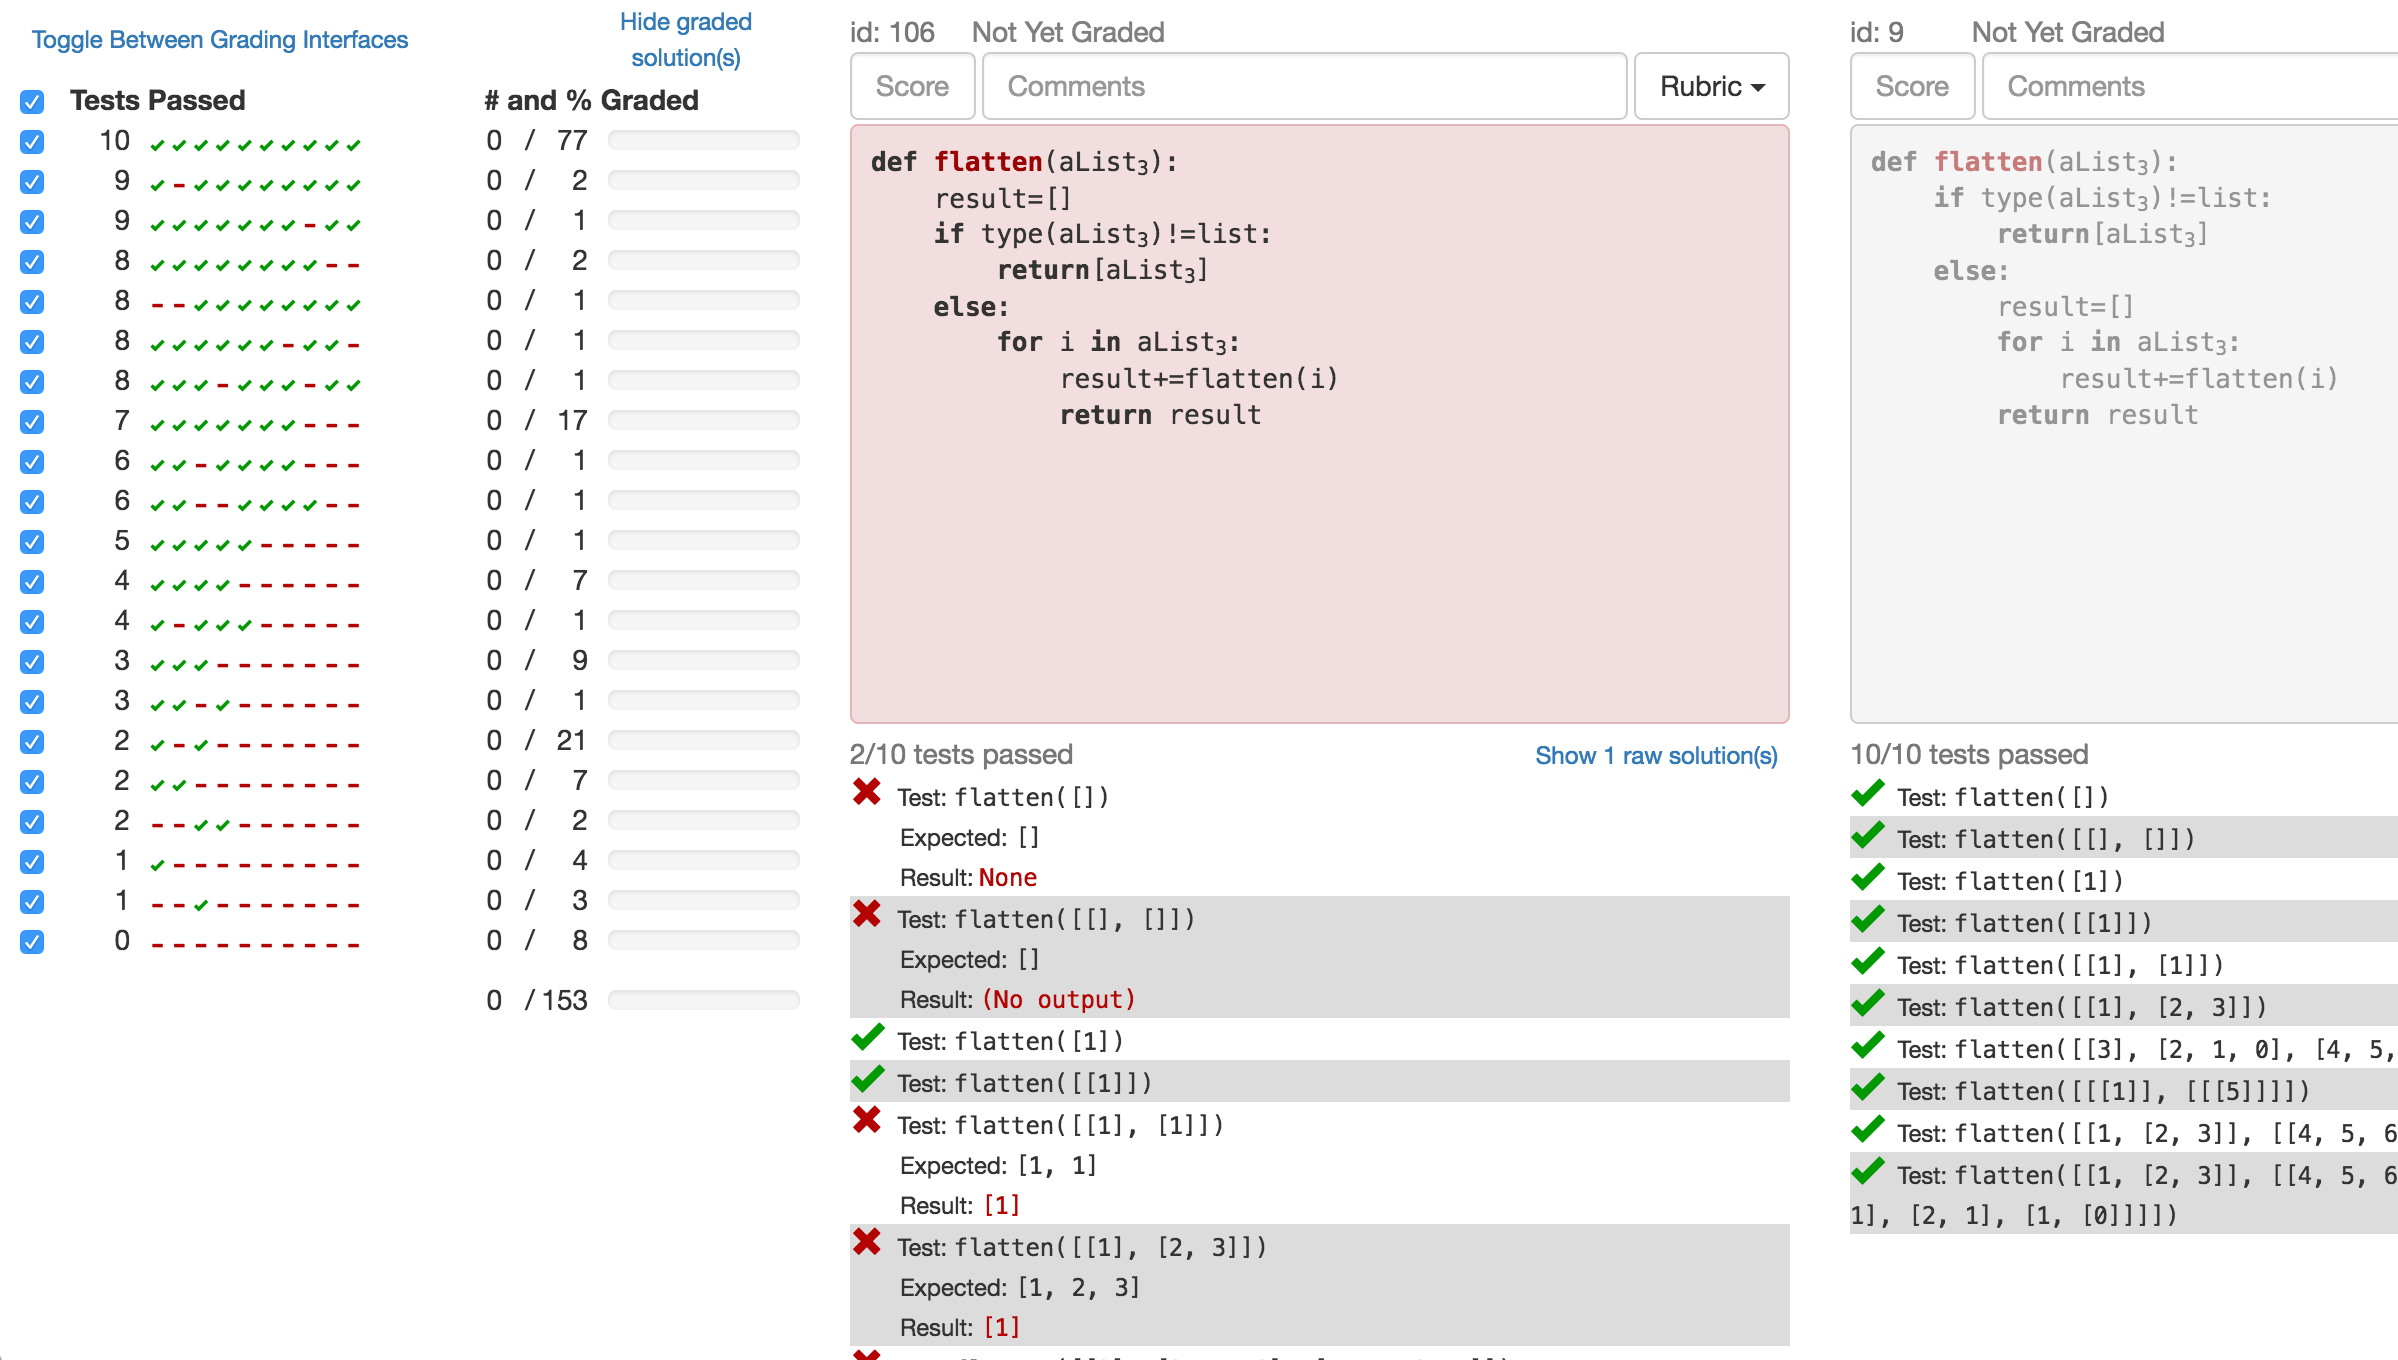
\includegraphics[width=\textwidth]{Body/figures/grovercode/figure_1}
\caption{\DIFaddFL{The GroverCode user interface displaying solutions to an introductory Python programming exam problem, in which students are asked to implement a function to flatten a nested list of arbitrary depth.
}}
\label{fig:whole_interface}
\end{figure} 

\begin{figure*}[t!]
    \centering
    \begin{subfigure}[b]{0.5\textwidth}
        \centering
        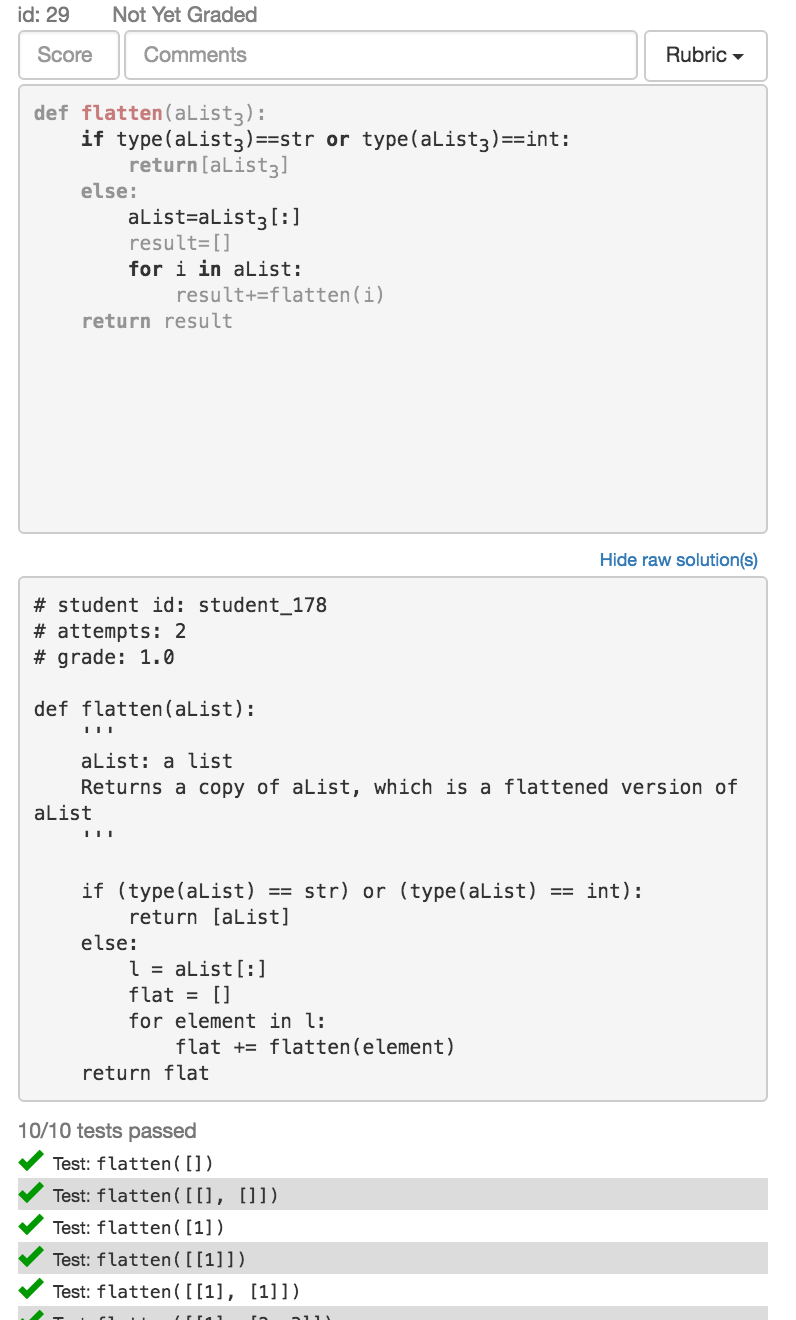
\includegraphics[height=4in]{Body/figures/grovercode/figure_2}
        \caption{\DIFaddFL{A correct solution, its corresponding raw solution, and its performance on test cases, as displayed in GroverCode.}}
        \label{fig:correct_stack}
    \end{subfigure}%DIF > 
    \DIFaddendFL ~ 
    \DIFdelbeginFL %DIFDELCMD < %DIFDELCMD < \label{subsec:morelineinfo}%%%
%DIFDELCMD < %%%
\DIFdelFL{It was also noticed that }\DIFdelendFL \DIFaddbeginFL \begin{subfigure}[b]{0.5\textwidth}
        \centering
        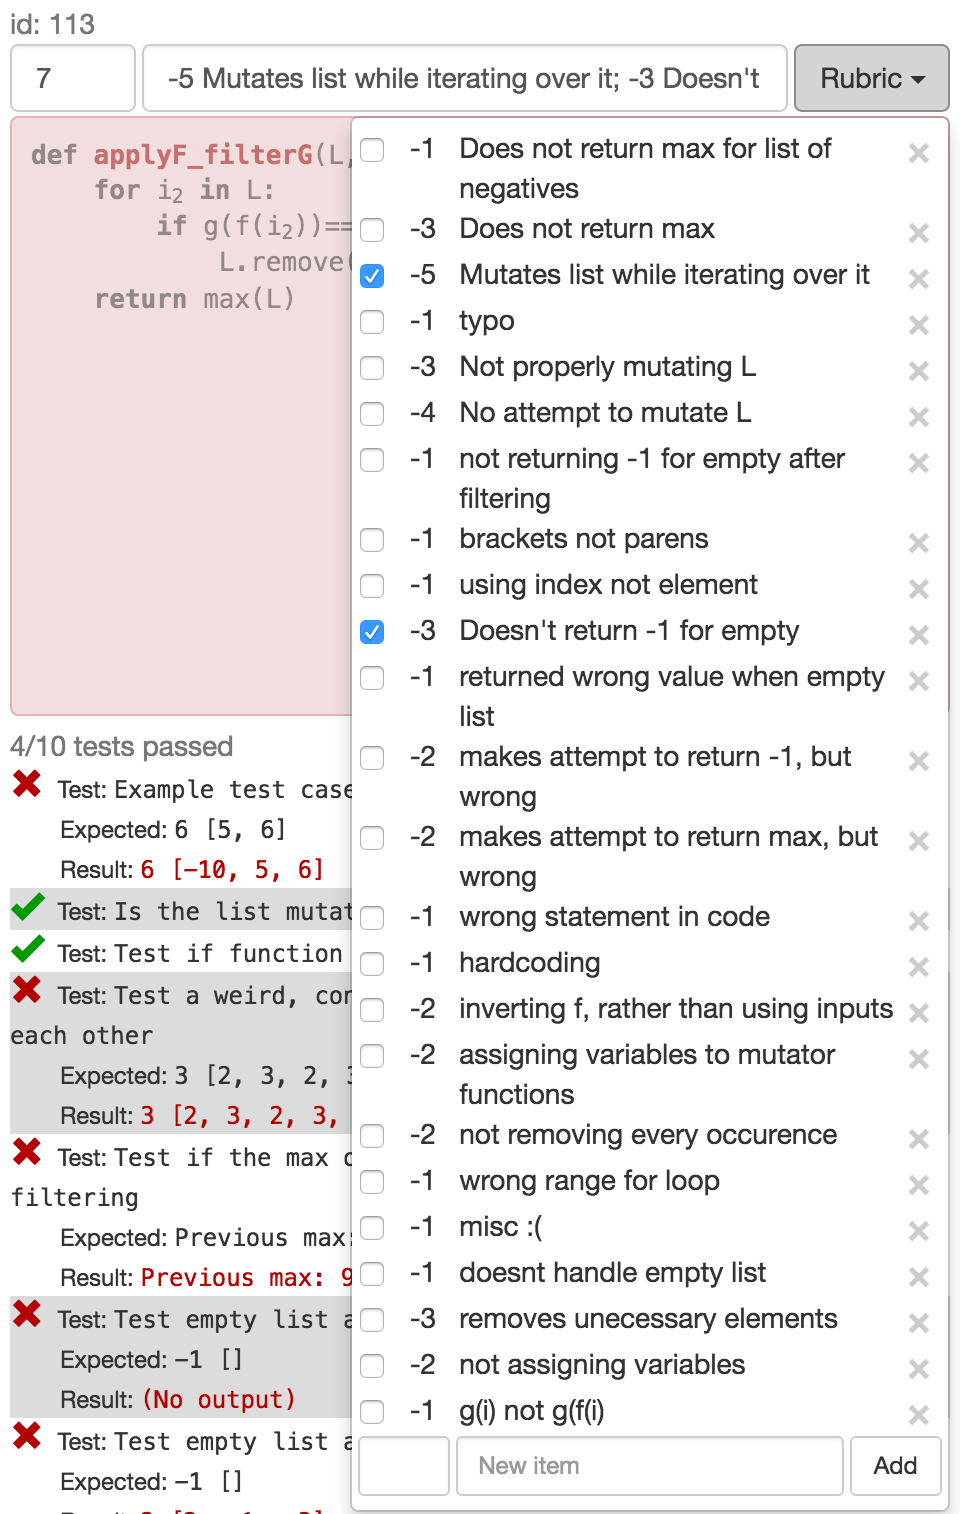
\includegraphics[height=4in]{Body/figures/grovercode/figure_3}
        \caption{\DIFaddFL{An incorrect solution with the rubric dropdown menu open. Text for each of the checked items is automatically inserted in the comment box.}}
        \label{fig:rubric}
    \end{subfigure}
    \caption{\DIFaddFL{Correct and incorrect solutions, as rendered by GroverCode.}}
\label{fig:correct_and_incorrect_stacks}
\end{figure*}

%DIF >  \begin{figure}
%DIF >  \centering
%DIF >  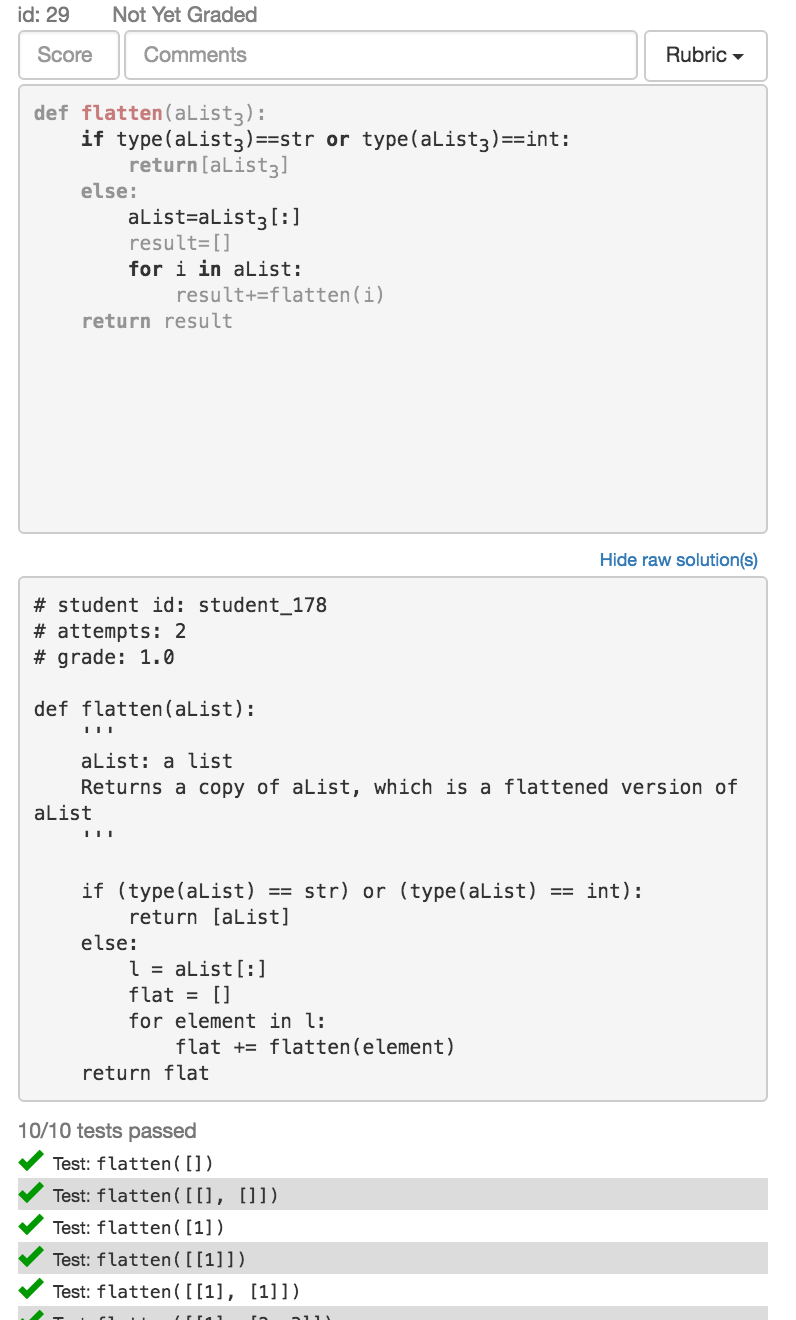
\includegraphics[width=0.5\textwidth]{Body/figures/grovercode/figure_2}
%DIF >  \caption{A correct solution, its corresponding raw solution, and its performance on test cases, as displayed in GroverCode.}
%DIF >  \label{fig:correct_stack}
%DIF >  \end{figure}

%DIF >  \begin{figure}
%DIF >  \centering
%DIF >  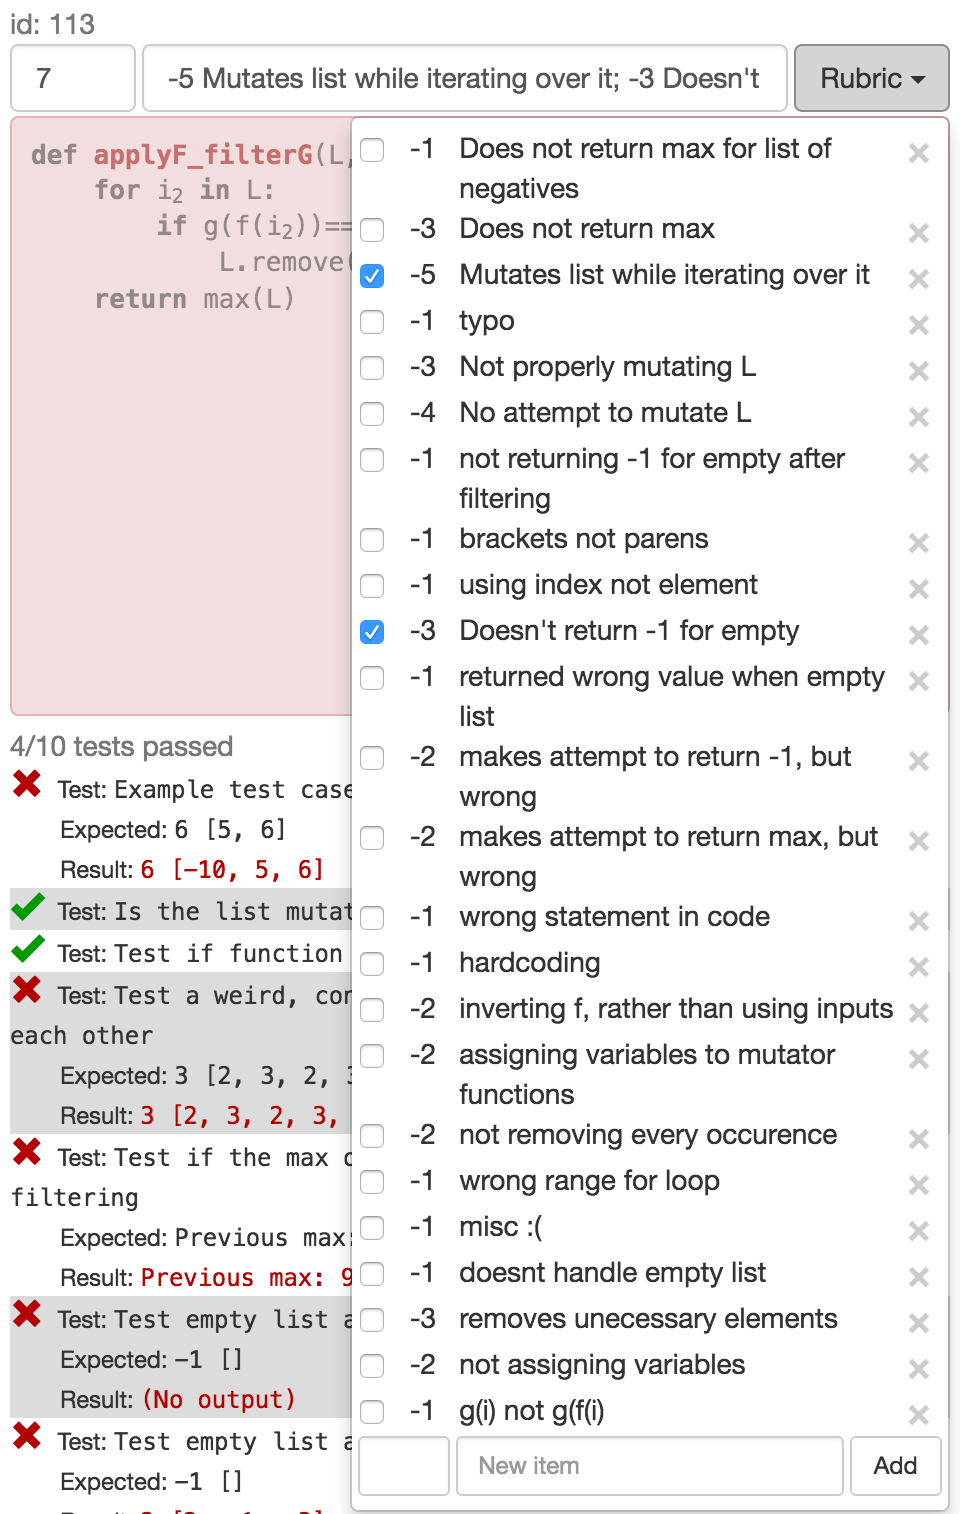
\includegraphics[width=0.5\textwidth]{Body/figures/grovercode/figure_3}
%DIF >  \caption{A stack with the rubric dropdown menu open. Text for each of the checked items is automatically inserted in the comment box.}
%DIF >  \label{fig:rubric}
%DIF >  \end{figure}

\DIFadd{The panel of progress indicators and filters, shown on the left side of Figure~\ref{fig:whole_interface}, helps teachers understand the distribution of solution behavior on test cases, track their grading progress, and grade sets of solutions that fail the same test cases one at a time. The rows of aligned sequences of green checks and red dashes represent error vectors, i.e., the pass/fail results with respect to the ordered list of teacher-specified test cases. The checkbox next to each error vector allows the teacher to selectively view subsets of solutions based on the particular tests they pass and fail. Solutions with the same error vectors may include similar mistakes. 
}

\DIFadd{Like OverCode, GroverCode groups correct solutions into stacks. Grades are propagated to all the solutions in a stack. Incorrect solutions were not also grouped into stacks because the stacking process was new and experimental for field deployment in an actual grading session. GroverCode still normalized all solutions, both correct and incorrect.
}

\DIFadd{The grading performed by the 6.0001 staff was intellectually demanding. For example, many staff members attempted to correct incorrect solutions by hand to better undertstand how far off the student was from a correct answer. When raw solutions are shown in random order, one solution may have a different approach, behavior, and appearance from the next. The transition from grading one solution to the next can mean starting from scratch. In an attempt to minimize the cognitive load of switching from one solution to the next, the GroverCode user interface includes the following features:
} \begin{itemize} 
\item \DIFadd{Horizontally aligned solutions for side-by-side comparison
}\item \DIFadd{Easy filtering of solutions by input-output behavior, i.e., their error vectors
}\item \DIFadd{Normalized variable names
}\item \DIFadd{Solutions ordered to minimize the distance between adjacent solutions with respect to a custom similarity metric defined in Stacey Terman's Master's of Engineering thesis~\mbox{%DIFAUXCMD
\cite{staceythesis}
}%DIFAUXCMD
}\item \DIFadd{Highlighted lines of code in each solution which differ from the previous solution in the horizontal list
} \end{itemize} 

\DIFadd{In OverCode, }\DIFaddend a single-line difference between two solutions could, by affecting a variable's behavior, cause the variable renaming process to propagate that difference as a variable name change throughout all the lines that mention the affected variable. This non-locality of difference made it harder to spot in the user interface where the actual syntactic difference between two \DIFdelbegin \DIFdel{canonicalized }\DIFdelend \DIFaddbegin \DIFadd{platonic }\DIFaddend solutions was. As a result, stacks are rendered in the \DIFaddbegin \DIFadd{GroverCode }\DIFaddend user interface slightly differently. \DIFdelbegin \DIFdel{Now, even if the canonicalized }\DIFdelend \DIFaddbegin \DIFadd{Even if the normalized }\DIFaddend variable names are different between two syntactically identical lines of code in two different stacks, if the variables take on the same sequence of values {\it just within that line of code}, it will not be highlighted as different in the user interface. Only the line with the syntactic difference will be highlighted.


\DIFdelbegin \DIFdel{In order to implement this , the modified }\DIFdelend \DIFaddbegin \subsubsection{Implementation}\DIFadd{~}\label{subsec:grovercodepipeline}

\DIFadd{The GroverCode implementation is a modification of the OverCode pipeline. Solutions which return an expected output for all test cases during the preprocessing step are categorized as correct, and all other solutions, having failed at least one test case, are categorized as incorrect. Correct solutions are normalized by the same process as was used in the original OverCode. 
}

\DIFadd{In the original OverCode pipeline for correct solutions, variable behavior is assumed to hold enough semantic information to be the sole basis on which variable names are normalized. GroverCode applies this rule to incorrect solutions as well, but only for variables whose behavior matches a common variable in the correct solutions. This step may be error prone. Incorrect solutions are known to be wrong with respect to input-output behavior, the behavior of the variables within them is suspect too, even if it happens to match a common variable in a correct solution. %DIF > if a variable in an incorrect solution has the same behavior as a common variable in the correct solutions, GroverCode will rename the variable in the incorrect solution so it matches the common variable's name in the correct solutions.
}

%DIF > However, this renaming strategy may change in future versions of GroverCode because, 

\DIFadd{In incorrect solutions, syntax, e.g., the operations applied to a variable, may be more helpful for normalizing variable names than behavior. For example, in an incorrect solution, a variable $i$ may be operated or depended on exactly the same way as a common variable in a correct solution. However, if an error somewhere else in the solution causes $i$ to behave differently, the original method of identifying common variables will be thrown off. %DIF > Based on this example, variables in incorrect solutions that are not already renamed based on behavior are renamed based on syntax.
}

\DIFadd{The OverCode pipeline is modified for GroverCode to capture this syntactic information. The modified }\DIFaddend pipeline examines the program trace collected during preprocessing and the AST for each solution and compiles the following information for each line of code in each solution:
 \begin{enumerate} 
\item a template, i.e., the line of code with variables replaced by blanks, e.g., \texttt{\underline{\hspace{1em}} += 1} and \texttt{for \underline{\hspace{1em}} in range(\underline{\hspace{1em}}):}
\item an ordered list of the common \DIFdelbegin \DIFdel{variables' behavior and their canonicalized }\DIFdelend \DIFaddbegin \DIFadd{variable behaviors and their normalized }\DIFaddend names corresponding to each blank in the line, e.g., the blank in \texttt{\underline{\hspace{1em}} += 1} can be associated with one of several common variables, depending on the rest of the solution
\item an ordered list of the sequences of values each blanked-out variable in the line took on during execution, e.g., the first blank in \texttt{for \underline{\hspace{1em}} in range(\underline{\hspace{1em}}):} might iterate through \texttt{1,2,3} while, with each visitation of this line during execution, the second blank stays constant at \texttt{[1,2,3],[1,2,3],[1,2,3]}
 \end{enumerate} 
Items 1 and 2 in this list together contain the information in the original \DIFdelbegin \DIFdel{canonicalized }\DIFdelend \DIFaddbegin \DIFadd{normalized }\DIFaddend lines in OverCode and information about the line's syntax, regardless of the variables \DIFdelbegin \DIFdel{' }\DIFdelend identities. Items 1 and 3 capture the information necessary to tell what the variable behavior is just within that one line and whether two lines in two different stacks will be highlighted as different from each other. %DIF <  is, without being affected a very similar concept, except it is more robust to non-local variations in variable behavior. For example, if the line of code \texttt{for ___ in range(___):}initialization of two common variables 
\DIFdelbegin %DIFDELCMD < 

%DIFDELCMD < %%%
\DIFdelend This information is also used for variable renaming in incorrect solutions\DIFdelbegin \DIFdel{, as described in Section~\ref{subsec:grovercodepipeline}}\DIFdelend .

\DIFdelbegin %DIFDELCMD < \begin{comment}
%DIFDELCMD < %%%
\DIFdelend \DIFaddbegin \begin{table}
\centering
%DIF > Copied with permission from Terman~\cite{staceythesis}}\todo{get explicit permission}
\begin{tabular}{l l r}
%DIF > \hline
 &  & {\bf \DIFaddFL{Location}} \\
{\bf \DIFaddFL{Example line of code}} & {\bf \DIFaddFL{Template}} & {\bf \DIFaddFL{of }\texttt{\DIFaddFL{exp}}} \\
\hline
\footnotesize{\texttt{def power(base, exp):}} & \footnotesize{\texttt{def power(\underline{\hspace{1em}}},\underline{\hspace{1em}}):} & \DIFaddFL{1 }\\
%DIF > \hline
\footnotesize{\texttt{while index <= exp:}} & \footnotesize{\texttt{while \underline{\hspace{1em}}<=\underline{\hspace{1em}}:}} & \DIFaddFL{1 }\\
%DIF > \hline
\footnotesize{\texttt{return 1.0*base*power(base, exp-1)}} & \footnotesize{\texttt{return 1.0*\underline{\hspace{1em}}*\underline{\hspace{1em}}*power(\underline{\hspace{1em}},\underline{\hspace{1em}}-1)}} & \DIFaddFL{3 }\\
%DIF > \hline
\footnotesize{\texttt{return base*power(base, exp-1)}} & \footnotesize{\texttt{return \underline{\hspace{1em}}*power(\underline{\hspace{1em}},\underline{\hspace{1em}}-1)}} & \DIFaddFL{2 }\\
%DIF > \hline
\footnotesize{\texttt{return power(base, exp-1)*base}} & \footnotesize{\texttt{return power(\underline{\hspace{1em}},\underline{\hspace{1em}}-1)*\underline{\hspace{1em}}}} & \DIFaddFL{1 }\\
%DIF > \hline
\footnotesize{\texttt{ans = base*power(base, exp-1)}} & \footnotesize{\texttt{\underline{\hspace{1em}}=\underline{\hspace{1em}}*power(\underline{\hspace{1em}},\underline{\hspace{1em}}-1)}} & \DIFaddFL{3 }\\
%DIF > \hline
\footnotesize{\texttt{if exp <= 0:}} & \footnotesize{\texttt{if \underline{\hspace{1em}}<=0:}} & \DIFaddFL{0 }\\
%DIF > \hline
\footnotesize{\texttt{if exp == 0:}} & \footnotesize{\texttt{if \underline{\hspace{1em}}==0:}} & \DIFaddFL{0 }\\
%DIF > \hline
\footnotesize{\texttt{if exp >= 1:}} & \footnotesize{\texttt{if \underline{\hspace{1em}} >= 1:}} & \DIFaddFL{0 }\\
%DIF > \hline
\footnotesize{\texttt{assert type(exp) is int and exp >= 0}} & \footnotesize{\texttt{assert type(\underline{\hspace{1em}}) is int and \underline{\hspace{1em}}>=0}} & \DIFaddFL{0, 1 }\\
%DIF > \hline
\end{tabular}
\caption{\textbf{\DIFaddFL{Example:}} \DIFaddFL{All templates and locations in which the abstract variable }\texttt{\DIFaddFL{exp}}\DIFaddFL{, the second argument to a recursive }\texttt{\DIFaddFL{power}} \DIFaddFL{function, appears. A location represents the index or indices of the blanks that the abstract variable occupies, where the first blank is index 0, the second is index 1, and so on. The second and third columns together form a template-location pair.}} 
\label{tab:templatelocation}
\end{table}
\DIFaddend 

\DIFdelbegin \DIFdel{For example, in the two examples of raw solutionsbelow, there is one syntactic difference: in the second solution }\DIFdelend \DIFaddbegin \DIFadd{The GroverCode normalization process uses this syntactic information, in addition to behavior, to identify and rename common variables. The line's template, e.g., }\texttt{\DIFadd{for }\underline{\DIFadd{\hspace{1em}}} \DIFadd{in }\underline{\DIFadd{\hspace{1em}}}\DIFadd{:}} \DIFadd{is the syntax of the line with variable names removed. For each common variable in correct solutions}\DIFaddend , \DIFdelbegin \texttt{\DIFdel{result}} %DIFAUXCMD
\DIFdel{is initialized as a float instead of an int. Given that, in Python, the difference between }\DIFdelend \DIFaddbegin \DIFadd{GroverCode counts how many times it appears in each template and in which location, represented as an index into the blanks in the template. Examples of templates and locations are shown in Table }\autoref{tab:templatelocation}\DIFadd{. If a yet-unrenamed variable in an incorrect solution appears in the exact same template-locations as a common variable in a correct solution, it will be renamed to match that common variable. If a variable in an incorrect solution is still not normalized, the counts of template-locations associated with each common variable in the correct solutions are used, as described in detail in Terman~\mbox{%DIFAUXCMD
\cite{staceythesis}}%DIFAUXCMD
, to infer the most likely common variable it could be renamed to, as long as a threshold for similarity is met. Otherwise, its original name is kept.
}





\subsubsection{Field Deployment}

\DIFadd{Approximately two hundred students were enrolled in 6.0001, and nine instructors used GroverCode to grade nearly all student solutions. %DIF > Seven programming problems of a variety of difficulties were graded over the course of these two sessions.
The GroverCode analysis pipeline was run on both the midterm and final exam problems from the Spring 2016 semester of 6.0001, which had approximately 200 students enrolled. These exams contained seven programming problems in total, and between 133 and 189 solutions per problem made it through the analysis pipeline to be displayed in the user interface. The midterm problem prompts were:
} \begin{itemize} 
\item \texttt{\DIFadd{power}} \DIFadd{(q4): Write a recursive function to calculate the exponential }\texttt{\DIFadd{base}} \DIFadd{to the power }\texttt{\DIFadd{exp}}\DIFadd{.
}\item \texttt{\DIFadd{give\_and\_take}} \DIFadd{(q5): Given a dictionary }\texttt{\DIFadd{d}} \DIFadd{and a list }\texttt{\DIFadd{L}}\DIFadd{, return a new dictionary that contains the keys of }\texttt{\DIFadd{d}}\DIFadd{. Map each key to its value in }\texttt{\DIFadd{d}} \DIFadd{plus one if the key is contained in }\texttt{\DIFadd{L}}\DIFadd{, and its value in d minus one if the key is not contained in }\texttt{\DIFadd{L}}\DIFadd{.
}\item \texttt{\DIFadd{closest\_power}} \DIFadd{(q6): Given an integer base and a target integer }\texttt{\DIFadd{num}}\DIFadd{, find the integer exponent that minimizes the difference between }\DIFaddend \texttt{\DIFdelbegin \DIFdel{float}%DIFDELCMD < }s %%%
\DIFdel{and }\DIFdelend \DIFaddbegin \DIFadd{num}} \DIFadd{and }\DIFaddend \texttt{\DIFdelbegin \DIFdel{int}\DIFdelend \DIFaddbegin \DIFadd{base}\DIFaddend } \DIFdelbegin \DIFdel{s can cause problems for novice Python students, such as accidental integer division, }\texttt{\DIFdel{1}} %DIFAUXCMD
\DIFdel{and }\DIFdelend \DIFaddbegin \DIFadd{to the power of exponent, choosing the smaller exponent in the case of a tie.
} \end{itemize} 
\DIFadd{The final problem prompts were:
} \begin{itemize} 
\item \texttt{\DIFadd{deep\_reverse}} \DIFadd{(q4): Write a function that takes a list of lists of integers }\texttt{\DIFadd{L}}\DIFadd{, and reverses }\texttt{\DIFadd{L}} \DIFadd{and each element of }\texttt{\DIFadd{L}} \DIFadd{in place.
}\item \texttt{\DIFadd{applyF\_filterG}} \DIFadd{(q5): Write a function that takes three arguments: a list of integers }\texttt{\DIFadd{L}}\DIFadd{, a function }\texttt{\DIFadd{f}} \DIFadd{that takes an integer and returns an integer, and a function }\DIFaddend \texttt{\DIFdelbegin \DIFdel{1.0}\DIFdelend \DIFaddbegin \DIFadd{g}\DIFaddend } \DIFdelbegin \DIFdel{are considered to be different values, and therefore the }\DIFdelend \DIFaddbegin \DIFadd{that takes an integer and returns a boolean. Remove elements from }\texttt{\DIFadd{L}} \DIFadd{such that for each remaining element }\texttt{\DIFadd{i}}\DIFadd{, }\texttt{\DIFadd{f(g(i))}} \DIFadd{returns }\texttt{\DIFadd{True}}\DIFadd{. Return the largest element of the mutated list, or -1 if the list is empty after mutation.
}\item \texttt{\DIFadd{MITCampus}} \DIFadd{(q6): Given the definitions of two classes: }\texttt{\DIFadd{Location}}\DIFadd{, which represents a two-dimensional coordinate point, and }\texttt{\DIFadd{Campus}}\DIFadd{, which represents a college campus centered at a particular }\texttt{\DIFadd{Location}}\DIFadd{, fill in several methods in the }\DIFaddend \texttt{\DIFdelbegin \DIFdel{result}\DIFdelend \DIFaddbegin \DIFadd{MITCampus}\DIFaddend } \DIFdelbegin \DIFdel{variables in each }\DIFdelend \DIFaddbegin \DIFadd{class, a subclass of }\texttt{\DIFadd{Campus}} \DIFadd{that represents a college campus with tents at various }\texttt{\DIFadd{Locations}}\DIFadd{.
}\item \texttt{\DIFadd{longest\_run}} \DIFadd{(q7): Write a function that takes a list of integers }\texttt{\DIFadd{L}}\DIFadd{, finds the longest run of either monotonically increasing or monotonically decreasing integers in }\texttt{\DIFadd{L}}\DIFadd{, and returns the sum of this run.
} \end{itemize} 
\DIFadd{For each problem processed during the field deployments, an example of a staff-written correct solution is included in the Appendix.
}

\DIFadd{Using the GroverCode user interface, nine instructors, including one lecturer and eight teaching assistants (TAs) graded these solutions as part of their official grading responsibilities. Stacey Terman, the Master's of Engineering student who implemented most of GroverCode, was one of these TAs. Solutions that did not successfully pass through the pipeline were graded by hand afterwards. TA grading events, e.g., adding or applying rubric items and point values to solutions, were logged. The observer (the author of this thesis) took extensive notes during each day-long grading session to capture spontaneous feature requests as well as bugs and complaints. 
}

%DIF > \begin{comment}
%DIF >  {\bf Programming Exam Problems}

%DIF > Given the increasing difficulty of these exam problems, the following numbers dropped between the midterm and the final: the number of students present to take the exam, the number of students who submitted any solution to a given problem before the test period ended, and the number of correct solutions that could be clustered.

\subsubsection{Pipeline Evaluation}

\DIFadd{The number of solutions submitted for each problem and the number that were successfully processed by the GroverCode pipeline is shown in Table~\ref{table:num_submissions}. Table~\ref{table:cluster_stats} captures the scale of the variation as well as some clustering statistics. Table~\ref{table:renametype} summarizes the counts of the various mechanims by which variables in incorrect solutions were normalized.
}

\begin{table}[h!]
\centering
\begin{tabular}{l r|r|r|r|r|r|r}
%DIF > \hline
& \multicolumn{3}{c}{Quiz} & \multicolumn{4}{c}{Final} \\
%DIF > \cline{2-8}
& \DIFaddFL{q4 }& \DIFaddFL{q5 }& \DIFaddFL{q6 }& \DIFaddFL{q4 }& \DIFaddFL{q5 }& \DIFaddFL{q6 }& \DIFaddFL{q7 }\\
\hline
\DIFaddFL{Submissions }& \DIFaddFL{193 }& \DIFaddFL{193 }& \DIFaddFL{193 }& \DIFaddFL{175 }& \DIFaddFL{173 }& \DIFaddFL{170 }& \DIFaddFL{165 }\\
\hline
\DIFaddFL{Mean lines per solution }& \DIFaddFL{9.9 }& \DIFaddFL{16.9 }& \DIFaddFL{19.8 }& \DIFaddFL{12.3 }& \DIFaddFL{20.9 }& \DIFaddFL{50.0 }& \DIFaddFL{41.8 }\\
\hline
\DIFaddFL{Solutions }& \DIFaddFL{186 }& \DIFaddFL{189 }& \DIFaddFL{168  }& \DIFaddFL{170 }& \DIFaddFL{166  }& \DIFaddFL{134 }& \DIFaddFL{133 }\\
\DIFaddFL{successfully processed }& \DIFaddFL{96\% }& \DIFaddFL{98\% }& \DIFaddFL{87\% }& \DIFaddFL{97\% }& \DIFaddFL{96\% }& \DIFaddFL{79\% }& \DIFaddFL{81\% }\\
%DIF > \hline
\end{tabular}
\caption{\DIFaddFL{Number of solutions submitted and successfully processed by GroverCode for each problem in the dataset. Reasons why a solution might not make it through the pipeline include syntax errors and memory management issues caused by students' inappropriate function calls.}}
\label{table:num_submissions}
\end{table}

\begin{table}[!ht]
\centering
\begin{tabular}{l r|r|r|r|r|r|r}
%DIF > \hline
& \multicolumn{3}{c}{Quiz} & \multicolumn{4}{c}{Final} \\
%DIF > \cline{2-8}
& \DIFaddFL{q4 }& \DIFaddFL{q5 }& \DIFaddFL{q6 }& \DIFaddFL{q4 }& \DIFaddFL{q5 }& \DIFaddFL{q6 }& \DIFaddFL{q7 }\\
\hline
\DIFaddFL{Correct solutions }& \DIFaddFL{182 }& \DIFaddFL{160 }& \DIFaddFL{94 }& \DIFaddFL{96 }& \DIFaddFL{49 }& \DIFaddFL{16 }& \DIFaddFL{12 }\\
 & \DIFaddFL{94\% }& \DIFaddFL{82\% }& \DIFaddFL{49\% }& \DIFaddFL{55\% }& \DIFaddFL{28\% }& \DIFaddFL{9\% }& \DIFaddFL{7\% }\\
\hline
\DIFaddFL{Incorrect solutions }& \DIFaddFL{4 }& \DIFaddFL{29 }& \DIFaddFL{74 }& \DIFaddFL{74 }& \DIFaddFL{117 }& \DIFaddFL{118 }& \DIFaddFL{121 }\\
\hline
\DIFaddFL{Test cases }& \DIFaddFL{10 }& \DIFaddFL{15 }& \DIFaddFL{25 }& \DIFaddFL{11 }& \DIFaddFL{10 }& \DIFaddFL{17 }& \DIFaddFL{28 }\\
\hline
\DIFaddFL{Distinct error signatures }& \DIFaddFL{6 }& \DIFaddFL{16 }& \DIFaddFL{36 }& \DIFaddFL{12 }& \DIFaddFL{38 }& \DIFaddFL{57 }& \DIFaddFL{42 }\\
\hline
\DIFaddFL{Correct stacks }& \DIFaddFL{40 }& \DIFaddFL{84 }& \DIFaddFL{93 }& \DIFaddFL{47 }& \DIFaddFL{46 }& \DIFaddFL{16 }& \DIFaddFL{12 }\\
\hline
\DIFaddFL{Stacks with > 1 }\DIFaddendFL solution \DIFdelbeginFL \DIFdelFL{will be given distinct names in the canonicalized solutions.
Now, r
}%DIFDELCMD < \begin{tabular}{cc} 
%DIFDELCMD < \begin{minipage}{0.4\linewidth}
%DIFDELCMD < \begin{lstlisting}[]
%DIFDELCMD < %%%
\DIFdelFL{def iterPower(base, exp) :
    result=}\DIFdelendFL \DIFaddbeginFL & \DIFaddFL{13 }& \DIFaddFL{18 }& \DIFaddendFL 1 \DIFdelbeginFL \DIFdelFL{i=}\DIFdelendFL \DIFaddbeginFL & \DIFaddFL{8 }& \DIFaddFL{2 }& \DIFaddendFL 0 \DIFdelbeginFL \DIFdelFL{while i < exp:
        result *= base
        i += 1
    return result
}%DIFDELCMD < \end{lstlisting}
%DIFDELCMD < \end{minipage}
%DIFDELCMD < %%%
\DIFdelendFL & \DIFdelbeginFL %DIFDELCMD < \begin{minipage}{0.4\linewidth}
%DIFDELCMD < \begin{lstlisting}[]
%DIFDELCMD < %%%
\DIFdelFL{def iterPower(base, exp):
    result=1
    i=}\DIFdelendFL 0 \DIFdelbeginFL \DIFdelFL{while i < exp:
        result *= base
        i += }\DIFdelendFL \DIFaddbeginFL \\
\hline
\DIFaddFL{Solutions in stacks }& \DIFaddFL{151 }& \DIFaddFL{94 }& \DIFaddFL{2 }& \DIFaddFL{57 }& \DIFaddFL{5 }& \DIFaddFL{0 }& \DIFaddFL{0 }\\
%DIF > \hline
\end{tabular}
\caption{\DIFaddFL{The degree of variation in input-output behavior and statistics about stack sizes.}}
\label{table:cluster_stats}
\end{table}

\begin{table}
\centering
\begin{tabular}{l c|c|c|c|c|c|c}
%DIF > \hline
& \multicolumn{3}{c}{Quiz} & \multicolumn{4}{c}{Final} \\
%DIF > \cline{2-8}
& \DIFaddFL{q4 }& \DIFaddFL{q5 }& \DIFaddFL{q6 }& \DIFaddFL{q4 }& \DIFaddFL{q5 }& \DIFaddFL{q6 }& \DIFaddFL{q7 }\\
\hline
\DIFaddFL{Variables in incorrect submissions }& \DIFaddFL{15 }& \DIFaddFL{149 }& \DIFaddFL{482 }& \DIFaddFL{289 }& \DIFaddFL{550 }& \DIFaddFL{559 }& \DIFaddFL{859 }\\
\hline
\DIFaddFL{Variables renamed based on values }& \DIFaddFL{14 }& \DIFaddFL{84 }& \DIFaddFL{266 }& \DIFaddFL{97 }& \DIFaddFL{246 }& \DIFaddFL{97 }& \DIFaddFL{187 }\\
\hline
\DIFaddFL{Variables renamed based on templates }& \DIFaddFL{0 }& \DIFaddFL{58 }& \DIFaddFL{166 }& \DIFaddFL{136 }& \DIFaddFL{264 }& \DIFaddFL{188 }& \DIFaddFL{489 }\\
\hline
\DIFaddFL{Variables not renamed }& \DIFaddendFL 1 \DIFdelbeginFL \DIFdelFL{return result * 1.0
}%DIFDELCMD < \end{lstlisting}
%DIFDELCMD < \end{minipage}
%DIFDELCMD < %%%
\DIFdelendFL \DIFaddbeginFL & \DIFaddFL{7 }& \DIFaddFL{50 }& \DIFaddFL{56 }& \DIFaddFL{40 }& \DIFaddFL{274 }& \DIFaddFL{183 }\\
%DIF > \hline
\DIFaddendFL \end{tabular}
\DIFdelbeginFL %DIFDELCMD < \end{comment}
%DIFDELCMD < %%%
\DIFdelendFL \DIFaddbeginFL \caption{\DIFaddFL{Statistics about variables renaming based on different heuristics in the GroverCode normalization process.}}
\label{table:renametype}
\end{table}
%DIF > \end{comment}
 \DIFaddend 

\DIFdelbegin \DIFdel{For clarity in the OverCode user interface, the modifiers appended to common variables to resolve Common/Common collisions are no longer capitalized letters. Instead, they are rendered in the interface as numerical subscripts indicating whether they are the second or third or fourth (etc. ) most frequently occurring common variable with that name across all the solutions in the collection analyzed}\DIFdelend \DIFaddbegin \subsubsection{Discussion}

\DIFadd{GroverCode was particularly appreciated on simpler problems where correct solutions were clustered together and graded by a single action. Under these conditions, the clustering capability GroverCode inherits from OverCode amplified teacher effort.
}

\DIFadd{Variable renaming was, for simpler programming problems, an invisible and possibly slightly confusing helping hand. One grader remarked, out loud: ``Why is everyone naming their iterator variable `i'?'' at which point he had to be reminded of the variable renaming process. 
}

\DIFadd{When applied to more complex solutions, the normalization process was at times more harmful than helpful for teacher comprehension. As solutions became more varied and structurally complex, graders started toggling off normalization because the renaming of variables, removal of comments, and formatting standardization was removing clues they needed in order to understand student intent.
}

\DIFadd{The feature for grouping solutions based on their behavior on test cases was appreciated regardless of solution complexity. While it was difficult to get direct feedback on the helpfulness of pair-wise difference highlighting and optimized solution ordering, graders heavily used and appreciated the ability to filter and grade solutions one error vector at a time. At least one grader remarked aloud that it seemed like many of the solution with the same error vector made similar mistakes. Therefore filtering by error vector may have been one of the stronger contributors to any hypothetical decreased cognitive load due to using GroverCode over the status quo of random assignment to solutions in a CSV file}\DIFaddend .

%DIF > \todo{DNHT: add to related work Appropriately chosen latent variable models have already been used in the past to model open-source code and answers to open-response mathematical questions.}
\DIFaddbegin 

\DIFaddend \section{Conclusion}
\DIFdelbegin \DIFdel{We have designed the OverCode }\DIFdelend \DIFaddbegin \DIFadd{OverCode is a novel }\DIFaddend system for visualizing thousands of Python programming solutions \DIFdelbegin \DIFdel{to help }\DIFdelend \DIFaddbegin \DIFadd{that helps }\DIFaddend teachers explore the variations among them. Unlike previous approaches, OverCode uses a lightweight static and dynamic analysis to generate \DIFaddbegin \DIFadd{platonic solutions that represent }\DIFaddend stacks of similar solutions \DIFdelbegin \DIFdel{and uses variable renaming to present cleaned solutions for each stack }\DIFdelend in an interactive user interface. It allows teachers to filter stacks by \DIFdelbegin \DIFdel{line occurrence }\DIFdelend \DIFaddbegin \DIFadd{normalized lines of code }\DIFaddend and to further merge different stacks by composing rewrite rules. \DIFdelbegin \DIFdel{Based on }\DIFdelend \DIFaddbegin \DIFadd{As observed in }\DIFaddend two user studies with \DIFaddbegin \DIFadd{a total of }\DIFaddend 24 current and potential teaching assistants, \DIFdelbegin \DIFdel{we found }\DIFdelend OverCode allowed teachers to more quickly develop a high-level view of students' understanding and misconceptions, and provide feedback that is relevant to more \DIFdelbegin \DIFdel{students' solutions. 
We believe an information visualization approach is necessary for teachers to explore the variations among solutionsat the scale of MOOCs, and OverCode is an important step towards that goal. }\DIFdelend \DIFaddbegin \DIFadd{student solutions. 
}\DIFaddend 

\DIFaddbegin \DIFadd{GroverCode, an extension of OverCode which handles incorrect solutions, is a new tool for triaging and hand-grading solutions. It was successfully deployed in the field as the tool for grading the midterm and final exams of MIT's 6.0001 course, ``Introduction to Computer Science and Programming in Python''. Based on teachers' appreciation of the interface over the existing alternatives, GroverCode will continue to be deployed in the field to ease the subjective psychological burden of grading hundreds of Python programs. %DIF > I believe an information visualization approach is necessary for teachers to explore the variations among solutions at the scale of MOOCs, and OverCode is an important step towards that goal.
%DIF > \todo{make sure evidence of teacher's appreciate is included}
}\DIFaddend \chapter{Foobaz: Feedback on Variable Names at Scale}\label{chapter:foobaz}

\DIFdelbegin \DIFdel{Current traditional feedback methods, such as hand-grading student code for substance and style, are labor intensive and do not scale. We created a user interface that addresses feedback at scale for a particular and important aspect of code quality: }\DIFdelend \DIFaddbegin \DIFadd{This chapter presents the second example of clustering, visualizing, and giving feedback on an aspect of student solutions, i.e., the variety of student-chosen }\DIFaddend variable names. \DIFdelbegin \DIFdel{We built this user interface on top of an existing back-end that distinguishes variables by their behavior in the program. Therefore ourinterface not only allows teachers to comment on poor variable names, they can comment on names that mislead the reader about the variable's role in the program.
We ran two user studies in which 10 teachers and 6 students created and received feedback , respectively. The interface helped teachers give personalized variable name feedback on thousands }\DIFdelend \DIFaddbegin \DIFadd{It is adapted and updated from a paper presented at the ACM Symposium on User Interface Software and Technology (UIST) in 2015~\mbox{%DIFAUXCMD
\cite{foobaz}}%DIFAUXCMD
. Pronouns like ``we'' and ``our'' refer to the coauthors of the UIST paper.
}

\DIFadd{When providing feedback on the substance and style }\DIFaddend of student solutions\DIFdelbegin \DIFdel{from an edX introductory programming MOOC. In the second study, students composed solutions to the same programming assignments and immediately received personalized quizzes composed by teachers in the previous user study. }%DIFDELCMD < 

%DIFDELCMD < \section{Introduction}
%DIFDELCMD < 

%DIFDELCMD < %%%
\DIFdel{Current traditional feedback methods for solutions to programming assignments include }\DIFdelend \DIFaddbegin \DIFadd{, the status quo is grading by hand. Unfortunately, }\DIFaddend hand-grading \DIFdelbegin \DIFdel{student code for substance and style. Unfortunately, those methods are }\DIFdelend \DIFaddbegin \DIFadd{is }\DIFaddend labor intensive, potentially inconsistent across graders, and \DIFdelbegin \DIFdel{do }\DIFdelend \DIFaddbegin \DIFadd{does }\DIFaddend not scale to the sizes associated with Massive Open Online Courses (MOOCs). \DIFdelbegin \DIFdel{The scaling difficulty is particularly important when considering that  some residential course enrollments at prominent universities, like }\DIFdelend \DIFaddbegin \DIFadd{Residential courses are also becoming massive. For example, }\DIFaddend UC Berkeley's \DIFaddbegin \DIFadd{introduction to programming, }\DIFaddend CS61A, \DIFdelbegin \DIFdel{are rising above the thousand-student mark }\DIFdelend \DIFaddbegin \DIFadd{has had more than a thousand students enrolled per semester~}\DIFaddend \cite{biggestClass}. Some Computer Science teachers, such as MIT's John Guttag and Ana Bell, are simultaneously teaching hundreds of students in residential programming courses and thousands of online students in MOOC versions \DIFaddbegin \DIFadd{of their courses}\DIFaddend .

Variable naming is a specific, important aspect of writing readable, maintainable code, and many teachers want to give feedback on it. The quality of a name is \DIFdelbegin \DIFdel{most easily }\DIFdelend \DIFaddbegin \DIFadd{best }\DIFaddend judged when its role within the surrounding code is known. However, at scale, teachers cannot read every solution. Programming education at scale opens up new challenges for processing and presenting thousands of solutions so that teachers can more easily view them. Teachers also cannot write comments on each solution. This difficulty motivates the creation of tools that help teachers give customized feedback\DIFdelbegin \DIFdel{to subsets of students for whom that feedback is relevant}\DIFdelend .

\DIFdelbegin \DIFdel{We introduce }\DIFdelend \DIFaddbegin \DIFadd{This chapter introduces }\DIFaddend Foobaz, a \DIFdelbegin \DIFdel{user interface }\DIFdelend \DIFaddbegin \DIFadd{system }\DIFaddend for giving tailored feedback on student variable names at scale. Foobaz enables teachers to explore and comment on the quality of student-chosen variable names, given the role the variables play in \DIFdelbegin \DIFdel{students' code (see Figure \ref{fig:figure2})}\DIFdelend \DIFaddbegin \DIFadd{student solutions}\DIFaddend . A variable's \DIFdelbegin \DIFdel{role }\DIFdelend \DIFaddbegin {\it \DIFadd{role}} \DIFaddend is a function of the sequence of values that the variable \DIFdelbegin \DIFdel{contains }\DIFdelend \DIFaddbegin \DIFadd{takes on }\DIFaddend during program execution. The variety of student-chosen variable names for each role makes evaluating every one prohibitive. Using Foobaz, the teacher can \DIFdelbegin \DIFdel{label }\DIFdelend \DIFaddbegin {\it \DIFadd{label}} \DIFaddend a small subset of good and bad names for each role \DIFdelbegin \DIFdel{. 
}\DIFdelend \DIFaddbegin \DIFadd{with judgments like ``too short'' or ``misleading.'' Figure \ref{fig:figure2} shows the teacher interface.
}\DIFaddend 

\DIFaddbegin \begin{figure*}
\centering
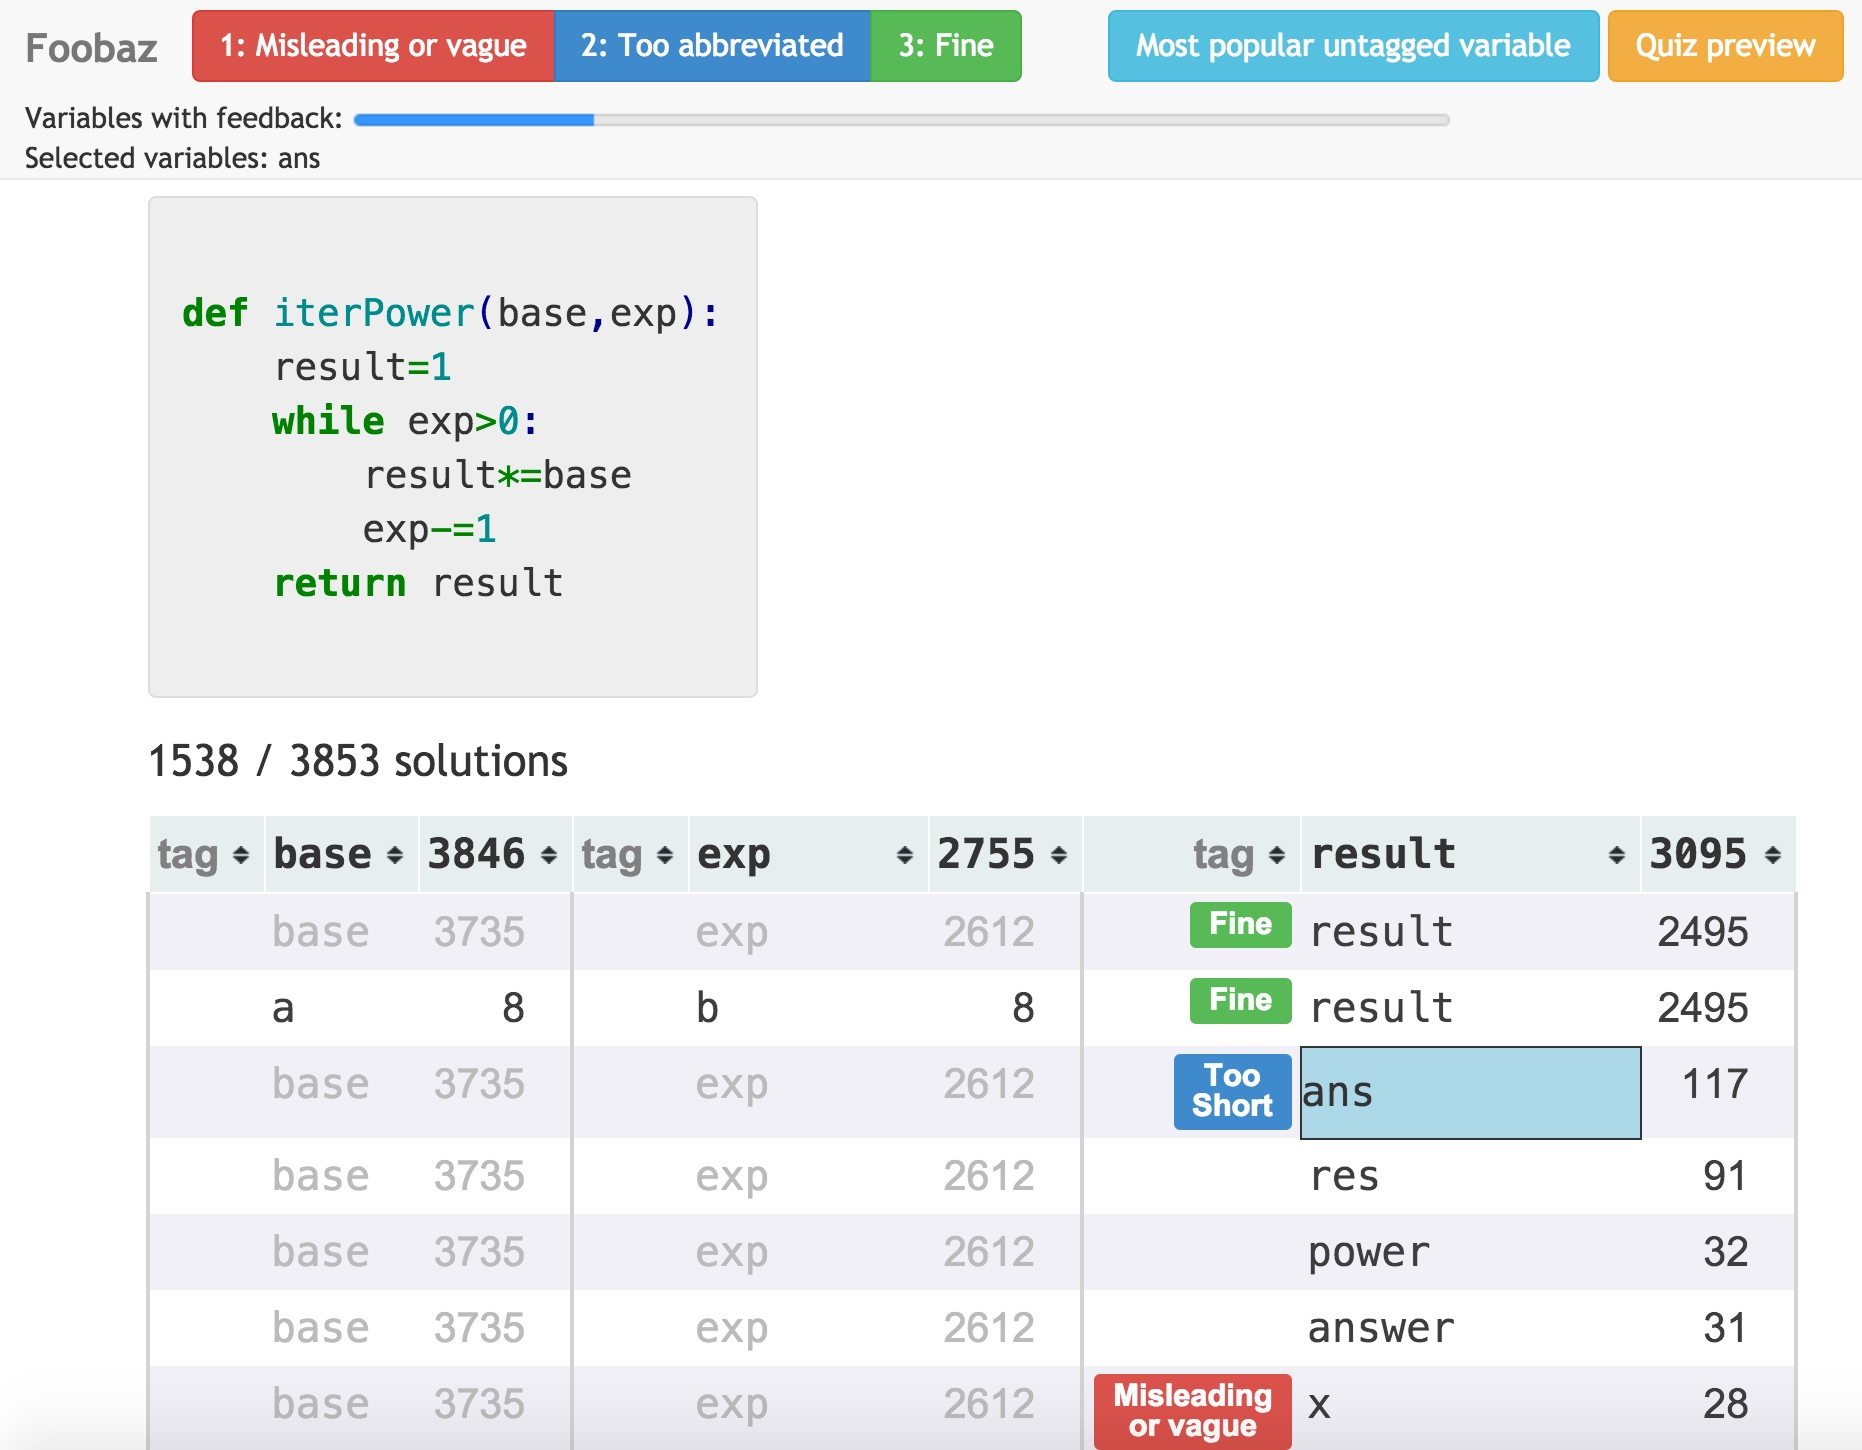
\includegraphics[width=0.75\linewidth]{Body/figures/foobaz/FoobazInitialView4.jpg}
\caption{\DIFaddFL{The Foobaz teacher interface. The teacher is presented with a scrollable list of normalized solutions, each followed by a table of student-chosen variable names. Some names shown here have been labeled by the teacher as ``misleading or vague,'' ``too short,'' or ``fine.''}}
\DIFaddFL{~}\label{fig:figure2}
\end{figure*}

\DIFaddend Foobaz then uses these labeled variable names to create pedagogically valuable active learning exercises in the format of multiple choice quizzes. These quizzes are a form of feedback for many more students than just those whose variable names receive a teacher \DIFdelbegin \DIFdel{'s label. The }\DIFdelend \DIFaddbegin \DIFadd{label. Rather than just receive a label on one of their own names, the }\DIFaddend quizzes also allow students to see examples of good and bad alternatives\DIFdelbegin \DIFdel{, rather than just receive a label on one of their own names. }\DIFdelend \DIFaddbegin \DIFadd{. This moves the feedback closer to the ideals described by variation theory.
}\DIFaddend 

\DIFdelbegin \DIFdel{Foobaz personalizes teacher quizzes for each student, }\DIFdelend \DIFaddbegin \DIFadd{Quizzes are personalized by Foobaz }\DIFaddend so that students \DIFdelbegin \DIFdel{can }\DIFdelend consider good and bad names for variables \DIFdelbegin \DIFdel{that exist }\DIFdelend \DIFaddbegin \DIFadd{with the same role }\DIFaddend in their own solutions. Personalized quizzes render the \DIFdelbegin \DIFdel{student's original code submission }\DIFdelend \DIFaddbegin \DIFadd{original student solution }\DIFaddend with a specific variable replaced by an arbitrary symbol. The quiz presents the student with several variable names as candidate replacements for the symbol, one of which may be the student's original choice. The student selects appropriate labels for the variable names before checking their labels against teacher labels\DIFdelbegin \DIFdel{and comments}\DIFdelend .

In two user studies, \DIFdelbegin \DIFdel{we demonstrate }\DIFdelend the capabilities and workflow enabled by this novel interface \DIFdelbegin \DIFdel{for both teachers and students. In the first study , we show }\DIFdelend \DIFaddbegin \DIFadd{are demonstrated. The first study shows }\DIFaddend that the interface helped teachers give personalized variable name feedback on thousands of student solutions from an introductory programming MOOC on edX. In the second study, students composed solutions to the same programming exercises and \DIFdelbegin \DIFdel{we capture their reactions to the }\DIFdelend \DIFaddbegin \DIFadd{received personalized }\DIFaddend quizzes generated with Foobaz by teachers in the first study.

%DIF > \todo{remove we from the rest of this chapter}
\DIFaddbegin 

\DIFaddend \section{User Interface}

\DIFdelbegin \DIFdel{Consider an introductory programming MOOC where thousands }\DIFdelend \DIFaddbegin \DIFadd{Thousands }\DIFaddend of students submit correct solutions to \DIFdelbegin \DIFdel{a programming exercise. Imagine that many }\DIFdelend \DIFaddbegin \DIFadd{the same programming problem in MOOCs and massive residential courses. Many }\DIFaddend of these solutions include \DIFdelbegin \DIFdel{a variable that takes }\DIFdelend \DIFaddbegin \DIFadd{variables that take }\DIFaddend on the same sequence of values \DIFdelbegin \DIFdel{, like a running sum of the elements in an input argument. While most students decide to name this variable $result$, others decide to give it obscure or less descriptive names like $p$, $val1$}\DIFdelend \DIFaddbegin \DIFadd{when run on the same test cases. Table~\ref{examplecommonvars} in Chapter~\ref{chapter:overcode} shows these common variables, the names students most commonly gave them, and some of the less common names for the same variables}\DIFaddend .

The quality of a variable's name is most easily judged when the teacher understands its algorithmic role and relationship to other variable names within the surrounding code. At scale, this can be difficult and frustrating, because while variable roles can be repetitive across many solutions\DIFdelbegin \DIFdel{(}\DIFdelend \DIFaddbegin \DIFadd{, their names can be unpredictable and vary greatly in quality, }\DIFaddend e.g., \DIFaddbegin \texttt{\DIFadd{result}}\DIFadd{, }\texttt{\DIFadd{val1}}\DIFadd{, or }\texttt{\DIFadd{s}} \DIFadd{as names for }\DIFaddend a particular running sum\DIFdelbegin \DIFdel{), their names can be unpredictable ($result$, $val1$, $s$)}\DIFdelend . Instead of \DIFdelbegin \DIFdel{browsing student submissions in a linear fashion, it would be better if the teacher }\DIFdelend \DIFaddbegin \DIFadd{giving feedback on variable names by browsing student solutions one by one, teachers }\DIFaddend could provide feedback on the basis of variable roles.

In Foobaz, teachers can browse \emph{stacks} of student \DIFdelbegin \DIFdel{submissions}\DIFdelend \DIFaddbegin \DIFadd{solutions represented by platonic solutions}\DIFaddend . A stack is a set of solutions whose code is identical after \DIFdelbegin \DIFdel{normalizing formattingand }\DIFdelend \DIFaddbegin \DIFadd{standardizing formatting, normalizing }\DIFaddend variable names, removing comments, and ignoring the exact order of statements. Within a stack, the teacher can browse the different sets of variable names that students chose, label some of them as, e.g., ``too short'' or ``misleading,'' and add comments. 

\DIFdelbegin \DIFdel{Teacher }\DIFdelend \DIFaddbegin \DIFadd{Foobaz uses teacher }\DIFaddend labels and comments \DIFdelbegin \DIFdel{are used }\DIFdelend to provide students with tailored feedback in the form of personalized quizzes on variable names. \DIFdelbegin \DIFdel{By providing feedback on only a few variable names , personalized quizzes are generated that are potentially relevant to thousands of students. }\DIFdelend \DIFaddbegin \DIFadd{A teacher only needs to label a few student-chosen names for the same variable role. Foobaz will then generate a quiz and every student whose solution contains that variable role can receive a personalized form of that quiz. %DIF > This quiz may be relevant to a significant fraction of students who submitted solutions.
}

%DIF > By providing feedback on only a few variable names, personalized quizzes are generated that are potentially relevant to thousands of students. 
\DIFaddend Foobaz is distinct from powergrading systems\DIFdelbegin \DIFdel{: instead }\DIFdelend \DIFaddbegin \DIFadd{. Instead }\DIFaddend of grading as many names as possible, \DIFdelbegin \DIFdel{the system produces personalized quizzes that have excellent examples }\DIFdelend \DIFaddbegin \DIFadd{teachers work with Foobaz to strategically label a small subset }\DIFaddend of good and bad \DIFdelbegin \DIFdel{variable names students would not otherwise get to see and learn from }\DIFdelend \DIFaddbegin \DIFadd{examples. If powergrading were possible, students might get feedback on their own variable name choices, but with Foobaz, they can learn from others' good and bad choices}\DIFaddend .

\subsection{Producing Stacks and Common Variables}
\DIFdelbegin \DIFdel{Foobaz enables feedback at scale because teachers can browse solutions on the basis of }\emph{\DIFdel{stacks of similar solutions}} %DIFAUXCMD
\DIFdel{and }\emph{\DIFdel{common variables}}%DIFAUXCMD
\DIFdel{. These groupings are automatically produced by the }\DIFdelend \DIFaddbegin \DIFadd{The }\DIFaddend OverCode analysis pipeline \DIFdelbegin \DIFdel{, which starts by executing each student 's }\DIFdelend \DIFaddbegin \DIFadd{executes each student }\DIFaddend solution on a \DIFdelbegin \DIFdel{single }\DIFdelend test case and \DIFdelbegin \DIFdel{tracking }\DIFdelend \DIFaddbegin \DIFadd{tracks }\DIFaddend the sequences of values that variables take on. Common variables are identified as those that behave the same way\DIFdelbegin \DIFdel{(}\DIFdelend \DIFaddbegin \DIFadd{, }\DIFaddend i.e., take on the same sequence of values\DIFdelbegin \DIFdel{) }\DIFdelend \DIFaddbegin \DIFadd{, }\DIFaddend across multiple solutions. \DIFdelbegin \DIFdel{Raw solutions are then normalized by renaming instances of common variables with their most popular names, as well as removing comments and extra whitespace. Normalized solutions that have the same set of lines can be grouped together into a }\emph{\DIFdel{stack}}%DIFAUXCMD
\DIFdel{, with a single representative on top for the teacher to read}\DIFdelend \DIFaddbegin \DIFadd{After executing every solution, the OverCode pipeline groups solutions into stacks of similar solutions. Each stack is represented by a single platonic solution. In the Foobaz teacher view, the teacher browses the platonic solutions and annotates the quality of variable names for common variables}\DIFaddend . 

The stacking performed by the system directly reduces the number of implementations that a teacher needs to analyze in order to provide feedback to the majority of the class. \DIFdelbegin \DIFdel{Furthermore, Foobaz is sensitive to }\emph{\DIFdel{variable roles}}%DIFAUXCMD
\DIFdel{, meaning that variables that }\DIFdelend \DIFaddbegin \DIFadd{Variables that }\DIFaddend behave the same across different stacks are linked together as a single common variable. The result is that feedback provided for a variable in one stack is propagated to variables that play out the same behavior in \emph{other} stacks.

\subsection{Rating Variable Names}

The Foobaz interface lets the teacher rate variable names in the context of their role in the program. Figure \ref{fig:figure2} shows the teacher \DIFdelbegin \DIFdel{'s }\DIFdelend view while they perform this task. 

The teacher is presented with a scrollable list of stacks. Each stack is represented as \DIFdelbegin \DIFdel{normalized stack code }\DIFdelend \DIFaddbegin \DIFadd{a platonic solution }\DIFaddend followed by a table of alternative variable names. Since some of the tables are taller than the screen, the \DIFdelbegin \DIFdel{normalized stack code }\DIFdelend \DIFaddbegin \DIFadd{platonic solution }\DIFaddend is pinned to the screen in such a way that it remains visible until the next stack is scrolled into view.

Each column of the table represents the common variables occurring in the stack, where each common variable's most popular name serves as the column header. Each row of the table represents a unique set of variable names used in a solution\DIFdelbegin \DIFdel{(e. g., $secretWord$, $lettersGuessed$, $guessedWord$, $char$)}\DIFdelend . \DIFaddbegin \DIFadd{For example, }\texttt{\DIFadd{secretWord}}\DIFadd{, }\texttt{\DIFadd{lettersGuessed}}\DIFadd{, }\texttt{\DIFadd{guessedWord}}\DIFadd{, and }\texttt{\DIFadd{char}} \DIFadd{are all the names that were used in one particular raw solution. }\DIFaddend We show \emph{sets} of variable name choices, rather than independent columns of variable names, because we found in early pilot testing that variable names can at times make more sense when seen as a group, rather than as individual naming decisions. This helps give teachers the context and confidence to assign quality judgments.

As the teacher brushes over the names of a common variable in the table, its occurrences in the \DIFdelbegin \DIFdel{normalized code }\DIFdelend \DIFaddbegin \DIFadd{platonic solution }\DIFaddend are highlighted, so they can develop an understanding of the variable's role in the solution. The teacher can then go down the list of student-chosen names, rating as many of them as they desire using three different labels: ``misleading or vague,'' ``too short,'' or ``fine.'' These labels were based on early pilot testing with beginner programmers but future iterations of Foobaz may support teacher-added labels. Next to each name, they can also see how frequently it was given to that common variable across all solutions in the dataset, and can sort the entire table by this frequency. In order to draw teachers' attention to student-chosen variable names, variables with names that match one of given parameter names provided with the homework prompt are greyed out. The long tail of infrequently used names can be a place where both the best and worst examples of names can be found.

It is important to note that each common variable is likely to occur in multiple stacks. When the teacher selects a particular name, or set of names, for a common variable, occurrences in other stacks are highlighted as well. When they assign a label to a name, the label is propagated to all uses of the name for that common variable, across all the stacks. This has the effect of ``filling down'' the teacher \DIFdelbegin \DIFdel{'s }\DIFdelend annotations. As teachers scroll down, they see that much of their feedback has been propagated for them, letting them focus on the remaining best and worst examples they might find. 

A progress bar at the top of the page indicates the coverage of their feedback across all variable names. Since teachers were motivated by the progress bar to maximize their coverage, we provided a button which would select and scroll into view the next most popular, yet unlabeled name for a common variable. Also included to maximize efficiency, the interface supports navigation through the variable names in the table using arrow keys. Teachers can also press hotkeys to rate variables instead of clicking on one of the three quality judgments, e.g., press \DIFdelbegin \DIFdel{$2$ }\DIFdelend \DIFaddbegin \texttt{\DIFadd{2}} \DIFaddend to rate a variable name as ``too short.''

\begin{figure}
\centering
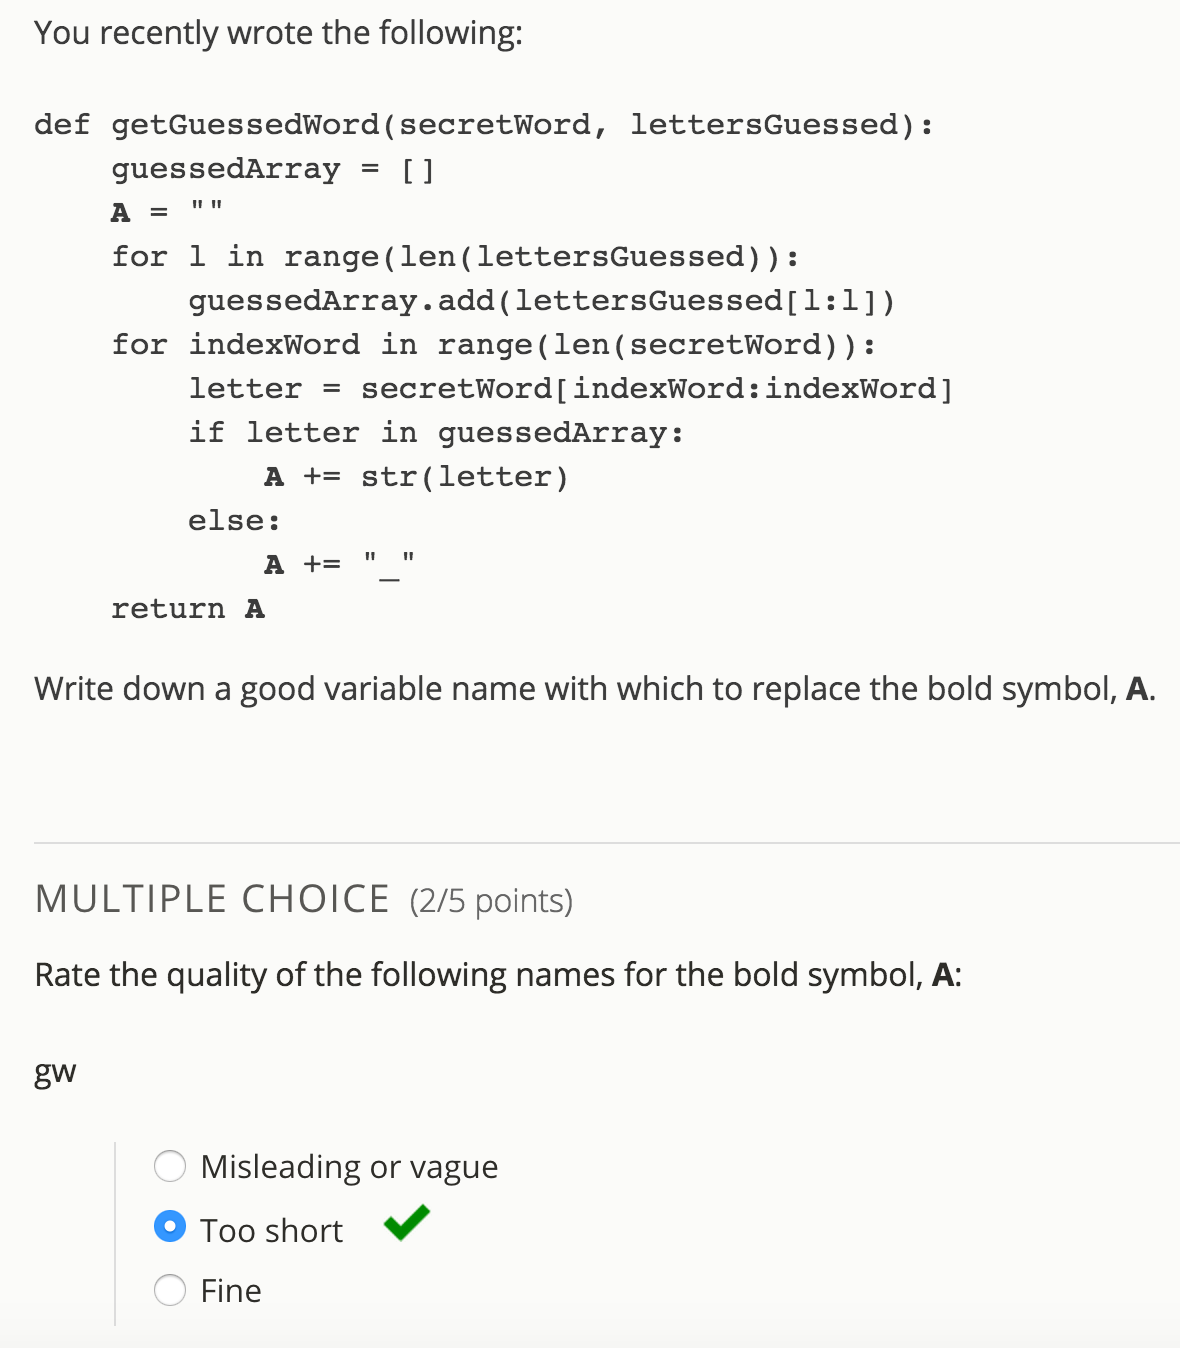
\includegraphics[width=0.95\columnwidth]{Body/figures/foobaz/feedbackQuizExample.png}
\caption{A personalized quiz as seen by the student, delivered by \DIFdelbeginFL \DIFdelFL{an edX-based system maintained by a large university}\DIFdelendFL \DIFaddbeginFL \DIFaddFL{edX infrastructure}\DIFaddendFL . \DIFdelbeginFL \DIFdelFL{Students are }\DIFdelendFL \DIFaddbeginFL \DIFaddFL{The student is }\DIFaddendFL shown their own code, with a variable name replaced by an arbitrary symbol, followed by variable names for the student to consider and label using the same labels that were available to the teacher. After the student has submitted their own judgments, the teacher \DIFdelbeginFL \DIFdelFL{'s }\DIFdelendFL labels are revealed, along with their explanatory comments.}~\label{fig:figure4}
\end{figure}

\begin{figure}
\begin{minipage}{1\columnwidth}
\centering
\DIFdelbeginFL %DIFDELCMD < 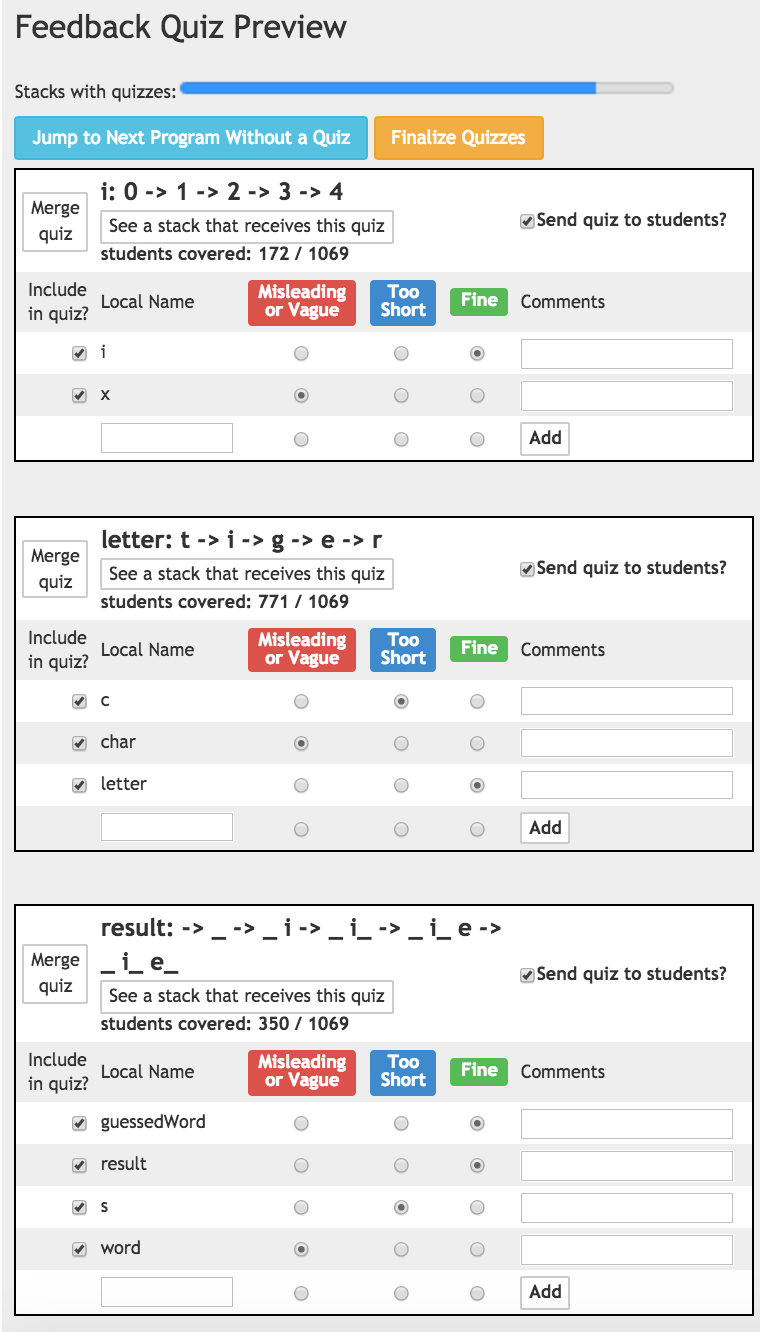
\includegraphics[width=0.85\columnwidth]{Body/figures/foobaz/quizPreviewHangman.png}
%DIFDELCMD < %%%
\DIFdelendFL \DIFaddbeginFL 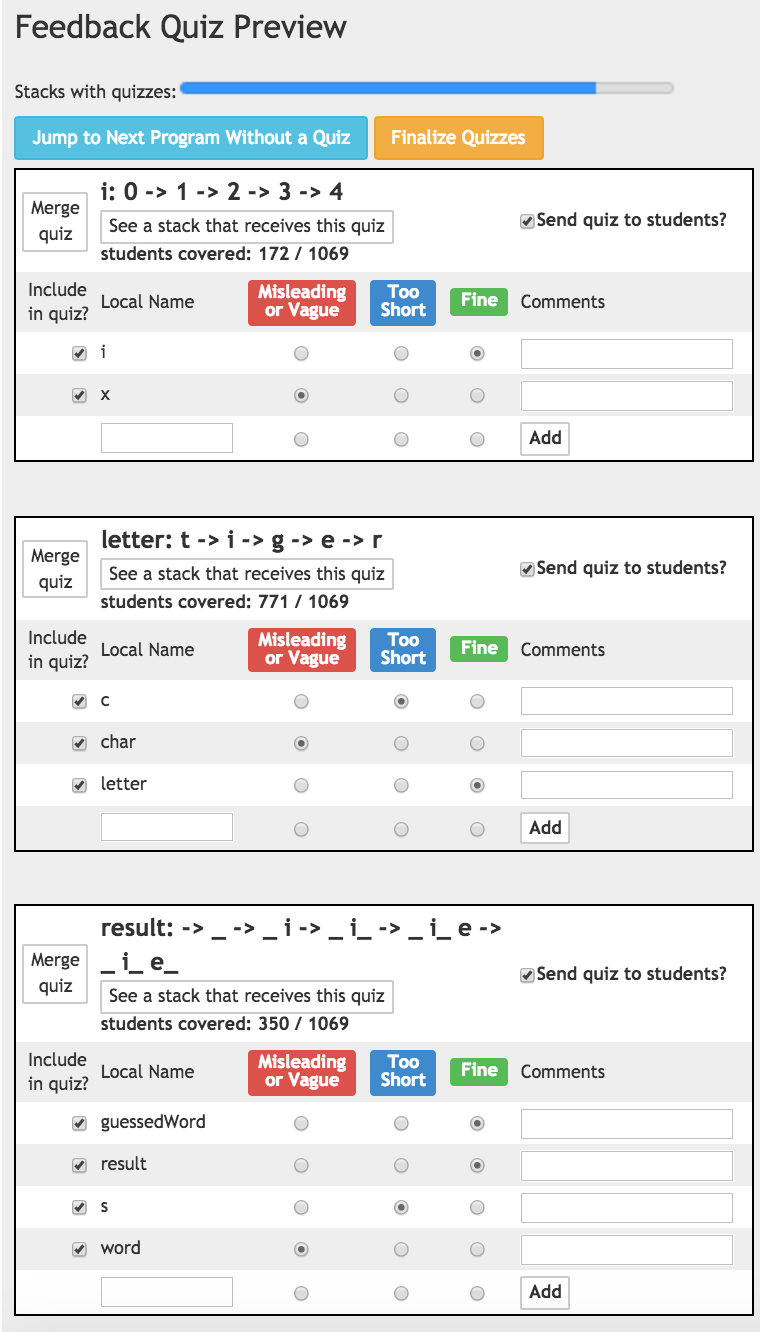
\includegraphics[width=0.7\columnwidth]{Body/figures/foobaz/quizPreviewHangman.png}
\DIFaddendFL \caption{The quiz preview pane of the Foobaz teacher interface. Variable behavior was logged by running all solutions on a common test case. This particular teacher created quizzes for the common variable \DIFdelbeginFL \DIFdelFL{$i$ }\DIFdelendFL \DIFaddbeginFL \texttt{\DIFaddFL{i}} \DIFaddendFL that iterates through indices of a list, the common variable \DIFdelbeginFL \DIFdelFL{$letter$}\DIFdelendFL \DIFaddbeginFL \texttt{\DIFaddFL{letter}}\DIFaddendFL , which iterates through the characters in an input string, and the common variable \DIFdelbeginFL \DIFdelFL{$result$}\DIFdelendFL \DIFaddbeginFL \texttt{\DIFaddFL{result}}\DIFaddendFL , which accumulates one of the acceptable return values, `\DIFdelbeginFL \DIFdelFL{$\_i\_e\_$}\DIFdelendFL \DIFaddbeginFL \texttt{\DIFaddFL{\_i\_e\_}}\DIFaddendFL .'}~\label{fig:figure3}
\end{minipage}
\DIFaddbeginFL \end{figure}
\DIFaddend 

\DIFdelbegin %DIFDELCMD < \bigskip
%DIFDELCMD < %%%
\DIFdelend \DIFaddbegin \begin{figure}
\DIFaddendFL \begin{minipage}{1\columnwidth}
\centering
\begin{tabular} {|l|l|r|}
\hline
\tabhead{Problem Description} & \tabhead{Source} & \tabhead{Solutions} \\ \hline \hline
\codevar{iterPower} & 6.00x (edX) & 3875 \\ \hline
\codevar{hangman} & 6.00x (edX) & 1118 \\ \hline
\codevar{computeDerivative} & 6.00x (edX) & 1433 \\ \hline
\codevar{dotProduct} & 6.0001 (residential) & 229 \\ \hline
\end{tabular}
\caption{Number of solutions in datasets.}
\label{solutioncounttable}
\end{minipage}

\bigskip
\begin{minipage}{1\columnwidth}
\centering
\begin{tabular}{|l|r|r|r|r|}
\hline
\tabhead{Problem} & \tabhead{Misleading} & \tabhead{Too short} & \tabhead{Good} & \tabhead{Total names} \\
& \tabhead{or Vague} & & & \\ \hline \hline
\codevar{iterPower} & 3 & 3 & 15 & 929 \\ \hline
\codevar{hangman} &7 & 4 & 10 & 763 \\ \hline
\codevar{compDeriv} & 6 & 5 & 10 & 670 \\ \hline
\codevar{dotProduct} & 11 & 3 & 17 & 180 \\ \hline
\end{tabular}
\caption{Subjects in \DIFdelbeginFL \DIFdelFL{Study 1}\DIFdelendFL \DIFaddbeginFL \DIFaddFL{the teacher study}\DIFaddendFL , on average, labeled a small fraction of the total names, covering all three provided name categories.}~\label{tab:averageLabeling}
\end{minipage}

\end{figure}

\subsection{Making Quizzes}

Each quiz is an active learning exercise that asks the student to think about good and bad names for a common variable. Quizzes begin by showing a solution with that common variable's name replaced by an arbitrary symbol everywhere it occurs. In a personalized quiz, the solution is the student's own, as shown in Figure \ref{fig:figure4}. The quiz presents the student with several variable names as candidate replacements for the symbol, one of which may be the student's original choice. The student labels these names before checking their labels against the teacher's. If a student \DIFdelbegin \DIFdel{'s }\DIFdelend solution includes a particular common variable, then that student can receive a personalized version of the quiz about that variable.

As teachers rate variables by attaching labels to them, quizzes are created with these names as their good and bad examples. Using the Toggle Quiz Preview button, teachers can see a preview of the quizzes (Figure \ref{fig:figure3}) alongside the scrollable list of stacks and watch the quizzes grow as they rate more names. They can hide the quiz preview to reduce visual clutter while they explore all the stacks, common variables, and interesting alternative names.

If two different common variables perform the same conceptual role in student solutions but do not go through the exact same sequence of values, then the teacher can use the ``Merge'' button to combine the quizzes about each common variable into a single quiz. This quiz becomes relevant to students who have either common variable in their own solution and can be sent out to both groups.

Ultimately, the teachers' goal is to provide pedagogically valuable personalized quizzes to as many of the hundreds or thousands of students in the course as possible. Analogous to the progress bar for variable names, the quiz preview pane includes a progress bar for the number of stacks of solutions that will receive at least one quiz. Like the previously discussed button for selecting the next most popular unlabeled name, the quiz preview pane also includes a button for jumping to the next largest stack of student solutions that do not yet have any quizzes. If the teacher deems one of their automatically populated quizzes to be not pedagogically valuable, then they can uncheck the option to send that quiz back to students. To provide more illustrative examples that might not have been produced in student solutions, teachers can add their own custom good and bad variable name examples and write explanations in the comment field associated with each alternative name.

\section{Evaluation}

We evaluate \DIFdelbegin \DIFdel{Foobaz's teacher and student-facing }\DIFdelend \DIFaddbegin \DIFadd{the Foobaz teacher and student }\DIFaddend interfaces with two consecutive user studies, one for each population. In order to evaluate \DIFdelbegin \DIFdel{Foobaz's scalability }\DIFdelend \DIFaddbegin \DIFadd{the scalability of Foobaz}\DIFaddend , the solutions seen by teachers were collected from MOOCs with thousands of students and a residential college class of several hundred students.

\subsection{Datasets}

We evaluated Foobaz on sets of correct solutions to four different programming \DIFdelbegin \DIFdel{exercises}\DIFdelend \DIFaddbegin \DIFadd{problems}\DIFaddend , ranging in size from a couple hundred to several thousand solutions, collected from 6.00x, an introductory programming course in Python that was offered on edX in the fall of 2012, and 6.0001, a residential introductory programming course in Python offered at MIT in the fall of 2014 (see Figure \ref{solutioncounttable}). The four exercises, referred to here as \codevar{iterPower}, \codevar{hangman}, \codevar{dotProduct}, and \codevar{computeDerivative}, are representative of typical exercises that students solve in the early weeks of an introductory programming course. They have varying levels of complexity and ask students to perform loop computation over three fundamental Python data types, integers, strings, and lists.

%DIF > \textbf{Power-law Distribution of Names} 
%DIF > The approximate power-law-type distribution of stacks from the thousands of edX solutions has already been reported in prior work, such as Figure 12 in \cite{overcode}. 
\DIFaddbegin 

\DIFadd{The distribution of unique combinations of variable names and behaviors does not differ significantly from a power-law distribution. The Kolmogorov-Smirnov test for a difference between the best-fitting power-law distribution and each dataset all gave p-values of at least $0.44$ (i.e., not significantly different), with the best-fitting exponent of the distribution between $1.79$ and $2.13$. Within each stack, the names for any particular variable appear to follow the same distribution.
}

\DIFadd{There is no ground truth for which variable names are ``bad,'' but we can report the counts of variables that the teachers chose to label and the counts of unique names for the top common variables in each problem. In the 3875 }\codevar{iterPower} \DIFadd{solutions, there were 179 different names given to a variable representing the base being exponentiated and 64 different names for a variable representing the exponent. In the 1393 }\codevar{computeDerivative} \DIFadd{solutions, there were 176 different names given for the variable containing the result and 39 different names for the most commonly used iterator variable. In the 1118 }\codevar{hangman} \DIFadd{solutions, there were 50 names given to the variable that iteratively takes on the characters of the secret word input argument and 99 names given to the variable containing the string most commonly returned by solutions as the answer.
}

\DIFaddend \subsection{Teacher Study}

\DIFaddbegin \DIFadd{The teacher study was designed to assess whether teachers could create variable name quizzes with the Foobaz teacher interface. If teachers could create quizzes, the study would measure how well those quizzes covered the student solutions in the dataset. These questions were answered by analyzing logs of each subject's activity while using Foobaz and their responses to survey questions about their experiences.
}

\DIFadd{The hour-long session contained a warm-up exercise, a Foobaz demonstration, and a session where subjects used Foobaz to create as many variable name quizzes for as many students as possible. }\DIFaddend During the initial briefing, teachers were informed that they would be looking at solutions that had already passed an autograder and instructed to focus only on variable names, ignoring other aspects of code style, structure, and correctness. Teachers \DIFdelbegin \DIFdel{were invited to look over a }\DIFdelend \DIFaddbegin \DIFadd{then attempt a warm-up exercise: composing variable name quizzes inspired by the variation in variable names they see in a baseline interface for viewing student solutions to problem $1$. They then watched a demonstration-based tutorial of Foobaz on student solutions to problem $2$, i.e., the training step. Finally they attempted to create variable name quizzes using the Foobaz interface for student solutions to problem $3$, i.e., the experimental condition. Over the course of the session, each teacher saw student solutions to three of the four possible problems, and counterbalancing was used to ensure that the same problems were not always being shown in the same interface. 
}

%DIF > \subsubsection{Warm-up}

\DIFadd{Before interacting with Foobaz, teachers worked on a control task. Teachers reviewed a }\DIFaddend page in a browser with all solutions concatenated in a random order into a flat list of boxed, syntax-highlighted code. \DIFaddbegin \DIFadd{This is the same baseline interface as was used in the OverCode Coverage Study. }\DIFaddend We chose this design as our baseline to emulate existing methods of reviewing student functions. 

Using this baseline interface, teachers were asked first to rate as many good and bad variable names as possible, with an eye toward maximizing coverage of names\DIFdelbegin \DIFdel{(Task Part 1). }\DIFdelend \DIFaddbegin \DIFadd{, i.e., Task Part 1. }\DIFaddend Next, the teachers were shown an example of a quiz and were asked to compose their own by listing variable names and labeling them as good or bad with whatever short descriptors and explanatory comments they wished\DIFdelbegin \DIFdel{(Task Part 2). }\DIFdelend \DIFaddbegin \DIFadd{, i.e., Task Part 2. }\DIFaddend Participants were given 5 minutes for each task, and then asked to fill out a survey about their experience. \DIFdelbegin \DIFdel{(}\DIFdelend The answers to two of these surveys were lost so we only report survey results from 8 of the 10 participants. 
\DIFdelbegin \DIFdel{)
}\DIFdelend 

\DIFaddbegin \DIFadd{The survey questions included both free response and 7-point Likert scale survey questions (1 means strong disagreement and 7 means strong agreement). The free response questions were:
} \begin{enumerate}  
\item \DIFadd{``What did you like about this process of providing feedback on variable names?''
}\item \DIFadd{``What did you NOT like about this process of providing feedback on variable names?'' 
}\item \DIFadd{``What did you wish you could have or achieve during this process of providing feedback on variable names?'' 
}\item \DIFadd{``What, if anything, did you find in the data that surprised you?''
} \end{enumerate} 
\DIFadd{The 7-point Likert scale survey questions were:
} \begin{enumerate} 
\item \DIFadd{``This interface helped me provide feedback to many students.''
}\item \DIFadd{``The interface helped me develop a high-level view of students' variable naming skills.''
}\item \DIFadd{``I saw a large percentage of these students' variable names.''
}\item \DIFadd{``I was able to give specific, personalized feedback to many students.''
}\item \DIFadd{``The system amplified my effort.''
} \end{enumerate} 

%DIF > \subsubsection{Experimental Condition}

\DIFaddend Participants learned about the Foobaz interface by watching a tutorial video. This training process took between 10 and 15 minutes depending on the dataset shown in the video. Participants were encouraged to hold their questions to the end, and answer them by interacting with the interface. 

Participants performed both Task Part 1 and 2 on a third dataset of solutions in the Foobaz teacher interface. Participants were asked to spend 5 minutes to perform each task, though some decided to spend more time. They filled out the same \DIFdelbegin \DIFdel{surveys }\DIFdelend \DIFaddbegin \DIFadd{survey }\DIFaddend about their experience again, followed by a final survey \DIFdelbegin \DIFdel{about which features of the Foobaz interface they found helpful}\DIFdelend \DIFaddbegin \DIFadd{with 7-point Likert scale questions about each Foobaz feature and Foobaz overall}\DIFaddend .

\subsubsection{Apparatus}

In all sessions, we used a laptop with a 15.4-inch 2880x1800 pixel Retina screen. All participants' interactions with the system were logged with timestamps\DIFdelbegin \DIFdel{using Meteor collections}\DIFdelend .

\subsubsection{Participants}

We recruited 10 participants (6 female) with ages between 20 and 29 ($\mu=23.1$, $\sigma=2.7$) through computer science-specific and campus-specific mailing lists and Facebook groups. All participants self-reported that they had been a grader, lab assistant, or teaching assistant for a Python course. 

\subsubsection{Results}

\textbf{Problems with Baseline} \DIFdelbegin \DIFdel{. }\DIFdelend When asked to comment on good and bad variable names based on the baseline interface, most teachers immediately began scrolling through solutions one by one, taking notes as they went, fully aware that they would only be able to skim a small, random fraction of the total number of solutions. The sheer volume of solutions was overwhelming to some. 

Results of the post-baseline survey reinforce critical usability issues with the status quo that Foobaz was designed to address. In these survey responses, teachers expressed an appreciation for the simplicity, readability, and searchability of the baseline interface but wished that the endless stream of often very similar solutions could be summarized or ``de-duped'' before they had to read through them. One teacher requested that variables be automatically identified, so that all references to a variable can be highlighted. This may have been a direct consequence of the fact that it was not possible to search for all the occurrences of the variable name \DIFdelbegin \DIFdel{$i$ }\DIFdelend \DIFaddbegin \texttt{\DIFadd{i}} \DIFaddend without the browser also highlighting all the \DIFdelbegin \DIFdel{$i$}\DIFdelend \DIFaddbegin \texttt{\DIFadd{i}}\DIFaddend 's within the rest of the names and keywords, e.g., the \DIFdelbegin \DIFdel{$i$ }\DIFdelend \DIFaddbegin \texttt{\DIFadd{i}} \DIFaddend in ``if.'' Another teacher requested an automated count of common variable names. These teachers anticipated three critical features of the Foobaz interface: deduplication, variable name counts, and highlighting all occurrences of selected names.

Two teachers commented on the importance of understanding the role a variable takes on within the program. One teacher writes, ``Many times the variable names meant something but I still had to read the code to make sure that it meant what I thought it meant in the context of the code.'' The second teacher observed, ``Whether a variable name is good or bad depends a lot on its function within the code, and since each code block has a somewhat unique structure, I felt like I should be creating separate categories for good vs. bad variables names, e.g., `for the derivative result,' `for a counter in a loop through poly,' etc.'' This is exactly what the Foobaz interface is designed to support. 

\DIFdelbegin \textbf{\DIFdel{Power-law Distribution of Names}}
%DIFAUXCMD
\DIFdel{The approximately power-law-type distribution of stacks of code from the thousands of edX solutions has already been reported in prior work, such as Figure 12 in \mbox{%DIFAUXCMD
\cite{overcode}}%DIFAUXCMD
. In Foobaz, the distribution of unique combinations of variable names and behaviors does not differ
significantly from a power-law distribution; the Kolmogorov-Smirnov test for a difference between the best-fitting power-law distribution and each dataset all gave p-values of at least $0.44$ (i. e., not significantly different), with }\DIFdelend \DIFaddbegin \DIFadd{Teachers did not respond strongly to the Likert scale questions about how much the interfaces helped them until after they used Foobaz. Specifically, after using the baseline interface, teachers did not strongly agree or disagree with the statement ``I was able to give specific, personalized feedback to many students'' ($\mu=3$, $\sigma = 1.4$ on a 7-point scale). Teachers slightly disagreed with the statement ``I saw a large percentage of these students' variable names'' ($\mu=2.6$, $\sigma=1.2$) and slightly agreed with the statement ``This interface helped me provide feedback to many students'' ($\mu=3.6$, $\sigma=2.0$). After using the Foobaz interface, }\DIFaddend the \DIFdelbegin \DIFdel{best-fitting exponent of the distribution between
$1.79$ }\DIFdelend \DIFaddbegin \DIFadd{mean level of agreement with these statements jumped to 5.5 ($\sigma=1.7$), 6.3 ($\sigma=0.46$), }\DIFaddend and \DIFdelbegin \DIFdel{$2.13$. Within each stack, the names for any particular variable appear to follow the same distribution.
}%DIFDELCMD < 

%DIFDELCMD < %%%
\DIFdel{There is no ground truth for which variable names are ``bad,'' but we can report the counts of variables that the users chose to label and the counts of unique names for the top common variables in each problem. In the 3875 }%DIFDELCMD < \codevar{iterPower} %%%
\DIFdel{solutions, there were 179 different names given to a variable representing the base being exponentiated and 64 different names for a variable representing the exponent. In the 1393 }%DIFDELCMD < \codevar{computeDerivative} %%%
\DIFdel{solutions, there were 176 different namesgiven for the variable containing the result and 39 different names for the most commonly used iterator variable. In the 1118 }%DIFDELCMD < \codevar{hangman} %%%
\DIFdel{solutions, there were 50 names given to the variable that iteratively takes on the characters of the `secret word' input argument and 99 names given to the variable containing the string most commonly returned by solutions as the answer. 
}%DIFDELCMD < 

%DIFDELCMD < %%%
\DIFdel{Figure \ref{tab:averageLabeling} shows the fraction of names that subjects labeled in Study 1, and the distribution of those names across various categories of quality. In spite of the unknown underlying distribution of good and bad variable names, the subjects are finding and labeling variables across all available categories in order to make quizzes}\DIFdelend \DIFaddbegin \DIFadd{6.6 ($\sigma=0.5$)}\DIFaddend .

\textbf{Efficiency of Foobaz} \DIFdelbegin \DIFdel{. }\DIFdelend The efficiency of using Foobaz to create feedback came up repeatedly in teachers' survey responses. Teachers appreciated the feeling of doing the task ``at scale.'' One teacher noted that it felt like, ``with each action, I was helping a large number of students'' without ``repeating or wasting effort too much.'' While using the button that highlights and scrolls the next most popular, untagged variable name into view, a teacher told the experimenter, ``I love this button!'' The arrow key-based navigation through tables of variable names was appreciated as well. At least one teacher commented that ``seeing variable names grouped by their role made the process much more efficient.'' 

The efficiency gains of the interface were hampered by, at times, a noticeably sluggish interface response time to some queries that scaled with the size of the dataset. This sluggishness \DIFdelbegin \DIFdel{can be cut down by reducing the many unnecessarily repeated calculationsmade in the current implementation.}\DIFdelend \DIFaddbegin \DIFadd{was significantly reduced by implementing the Foobaz teacher interface in a templating language instead than d3.js, precalculating variable name counts, and removing repeated calculations.%DIF >  as possible.%can be cut down by reducing the repeated calculations made in the current implementation.
}\DIFaddend 

\textbf{Quiz Composition} \DIFdelbegin \DIFdel{. }\DIFdelend In both interfaces, teachers appreciated the potential pedagogical value of making quizzes: ``I \DIFdelbegin \DIFdel{… }\DIFdelend \DIFaddbegin \DIFadd{... }\DIFaddend liked that with the [quiz] I made, students can actually learn about good alternatives. ... [T]hey can change their variable names after putting extra thought into it.'' A teacher expressed appreciation that, using the Foobaz interface, they could generate quizzes based on actual submitted code as well as their own comments. 

\DIFdelbegin \textbf{\DIFdel{Coverage}}%DIFAUXCMD
\DIFdel{. Immediately after using the baseline interface, teachers did not strongly agree or disagree with the statement ``I was able to give specific, personalized feedback to many students'' ($\mu =3$, $\sigma = 1.4$ on a 7-point Likert scale with 1: strong disagreement and 7: strong agreement). Teachers slightly disagreed with the statement ``I saw a large percentage of these students' variable names '' ($\mu=2.6$, $\sigma = 1.2$) and slightly agreed with the statement ``This interface helped me provide feedback to many students'' ($\mu=3.6$, $\sigma = 2.0$).After using the Foobaz interface, the mean level of agreement with these statements jumped to 5.5 ($\sigma = 1.7$), 6.3 ($\sigma = 0.46$), and 6.6 ($\sigma = 0.5$)}\DIFdelend \DIFaddbegin \DIFadd{In spite of the unknown underlying distribution of good and bad variable names, the teachers find and label variables across all available categories in order to make quizzes. Figure \ref{tab:averageLabeling} shows that teachers labeled only a small fraction of the total number of unique names and still found multiple examples for each of the categories of quality, i.e., misleading/vague, too short, and fine/good}\DIFaddend .

\DIFdelbegin \DIFdel{Figure \ref{fig:comboquizcoverage} shows that most }\DIFdelend \DIFaddbegin \textbf{\DIFadd{Coverage}} \DIFadd{Most }\DIFaddend solutions in the edX datasets received at least one or two quizzes\DIFdelbegin \DIFdel{. Solutions }\DIFdelend \DIFaddbegin \DIFadd{, as shown }\DIFaddend in Figure \ref{fig:comboquizcoverage}\DIFdelbegin \DIFdel{have multiple common variables on which they could potentially be quizzed (3, 3, and 4 on average in subfigures (a ), (b), and (c), respectively).
One teacher }\DIFdelend \DIFaddbegin \DIFadd{. Figure \ref{fig:variableCoverage} illustrates that, within minutes of their first interaction with the system, a teacher can label a significant portion of student-chosen variable names in a dataset. Their progress trails off as they encounter the long tail of names for particular roles and transition to creating better quizzes.
}

\DIFadd{Due to technical difficulties, only one of the ten teachers }\DIFaddend used Foobaz to create quizzes for \DIFdelbegin \DIFdel{a much smaller }\DIFdelend \DIFaddbegin \DIFadd{the 6.0001 }\DIFaddend dataset, collected from the residential class of only several hundred students. They achieved a similar percentage of coverage\DIFdelbegin \DIFdel{(}\DIFdelend \DIFaddbegin \DIFadd{, i.e., }\DIFaddend 87\% of student solutions received at least one quiz\DIFdelbegin \DIFdel{) }\DIFdelend \DIFaddbegin \DIFadd{, }\DIFaddend in a similar amount of time, showing that the Foobaz workflow and output \DIFdelbegin \DIFdel{appears }\DIFdelend \DIFaddbegin \DIFadd{may be }\DIFaddend relatively invariant to the size of the dataset.
\DIFdelbegin \DIFdel{Figure \ref{fig:variableCoverage} illustrates that, within minutes of their first interaction with the system, teachers can label a significant portion of student-chosen variable names in a dataset, though their progress trails off as they encounter the long tail of names for particular roles and transition to creating better quizzes.
}\DIFdelend 

Combined with Figure \ref{tab:averageLabeling}, Figure \ref{fig:comboquizcoverage} also shows that, by only labeling approximately 20 variable names in each of the edX datasets with thousands of student solutions, teachers cover at least 85\% of the class with personalized feedback quizzes. Even though Figure \ref{fig:variableCoverage} shows that the coverage of individual variable names with feedback is high, it matters less for Foobaz than in powergrading systems. What matters more is the coverage of students with quizzes that have \DIFdelbegin \DIFdel{excellent }\DIFdelend examples of good and bad variable names students would not otherwise get to see and learn from.

\begin{figure}
\begin{minipage}{1\columnwidth}
\centering
\DIFdelbeginFL %DIFDELCMD < 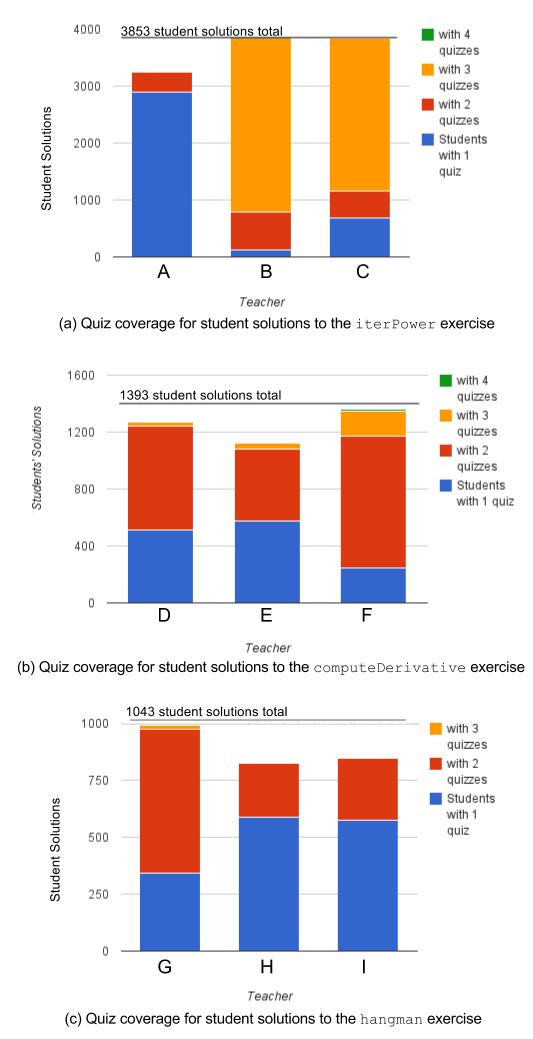
\includegraphics[width=1.0\columnwidth]{Body/figures/foobaz/ComboQuizCoverageFigure2.png}
%DIFDELCMD < %%%
\DIFdelendFL \DIFaddbeginFL 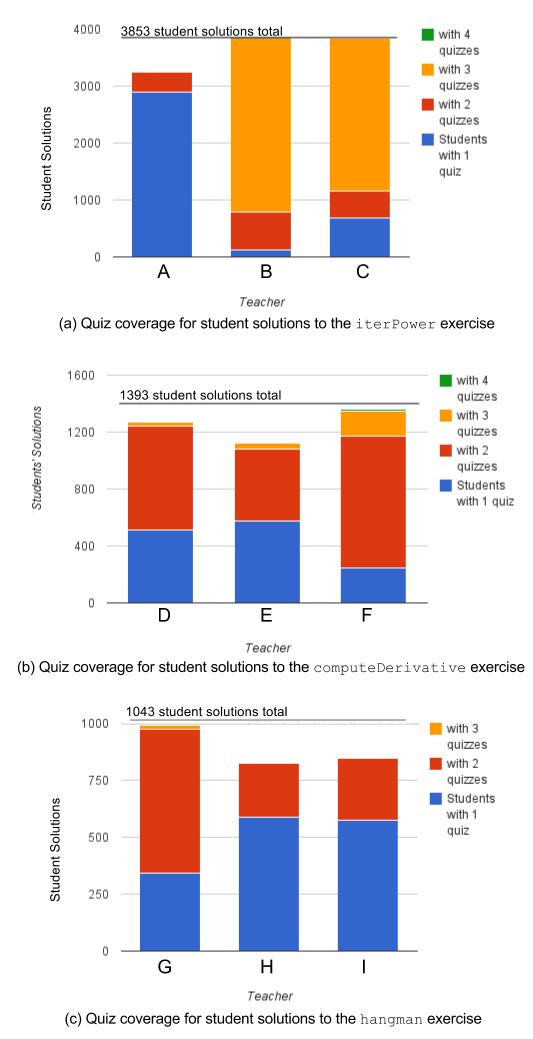
\includegraphics[width=0.7\columnwidth]{Body/figures/foobaz/ComboQuizCoverageFigure2.png}
\DIFaddendFL \caption{Quiz coverage of student solutions across three datasets.}~\label{fig:comboquizcoverage}
%DIF < \end{figure}
\DIFdelbeginFL %DIFDELCMD < \end{minipage}
%DIFDELCMD < %%%
\DIFdelendFL 

\DIFaddbeginFL \end{minipage}
\end{figure}
\begin{figure}
\DIFaddendFL \begin{minipage}{1\columnwidth}
%DIF < \begin{figure}
\DIFaddbeginFL 

\DIFaddendFL \centering
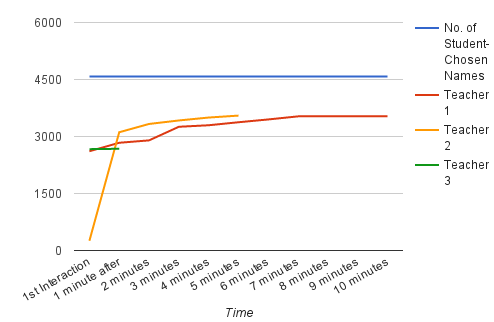
\includegraphics[width=0.9\columnwidth]{Body/figures/foobaz/variableCoverageNoTitle.png}
\caption{Variables in \DIFdelbeginFL \DIFdelFL{iterPower }\DIFdelendFL \DIFaddbeginFL \texttt{\DIFaddFL{iterPower}} \DIFaddendFL solutions labeled by each teacher.}~\label{fig:variableCoverage}
\end{minipage}
\end{figure}



\subsection{Student Study}

We ran a second study on the student side of the workflow in order to (1) find out if the teachers' efforts in the previous study produces quizzes that are relevant to these new students and (2) better understand student reactions to this novel form of feedback. In order to do this, we targeted beginner programming students and invited them into the lab \DIFaddbegin \DIFadd{for a one-hour session }\DIFaddend to receive personalized quizzes generated by the teachers in our previous study. \DIFaddbegin \DIFadd{Two experimenters, including the author of this thesis, separately ran students through the study in parallel, using two different machines.
}\DIFaddend 

Before the start of the study, quizzes composed by teachers using Foobaz in the first user study were rendered using the edX framework, ready to be personalized. Since pilot testing with beginner programming students indicated that six alternative variable names in a quiz is too many, teachers' quizzes were randomly subsampled to include a maximum of five alternative names for students to consider. 

Students came into the lab for one hour and composed solutions to one of the four exercises. After receiving each solution, the experimenter mentally executed the solution and compared the behavior of its variables to the variable behavior covered by the teachers' quizzes. If there was a match to one or more teachers' quizzes, one quiz was randomly selected. 
\DIFaddbegin 

\DIFadd{While quiz personalization is now automated, during the study this feature was demonstrated to subjects using the wizard of oz technique. }\DIFaddend The experimenter made a copy of the student \DIFdelbegin \DIFdel{'s code }\DIFdelend \DIFaddbegin \DIFadd{solution }\DIFaddend and replaced every instance of the variable to be quizzed on by an arbitrary symbol, \DIFdelbegin \DIFdel{e.g.}\DIFdelend \DIFaddbegin \DIFadd{i.e.}\DIFaddend , a bold letter \DIFdelbegin \DIFdel{A}\DIFdelend \DIFaddbegin {\bf \DIFadd{A}}\DIFaddend . The experimenter then appended the quiz to the modified copy of the student \DIFdelbegin \DIFdel{'s }\DIFdelend solution and delivered it to the student as a personalized quiz. If there was no match to one or more teachers' quizzes, then the student received a generic quiz, about a variable name in a solution other than their own.

After the student completed their personalized quizzes, they took a survey about their experience. Students who \DIFdelbegin \DIFdel{were able to complete }\DIFdelend \DIFaddbegin \DIFadd{completed }\DIFaddend the coding exercise and quizzes with significant time left in their \DIFaddbegin \DIFadd{one-hour }\DIFaddend session repeated this process for a second programming \DIFdelbegin \DIFdel{assignment}\DIFdelend \DIFaddbegin \DIFadd{problem}\DIFaddend .

\subsubsection{Apparatus}

In all sessions, we used laptops with 15.4-inch or 13.3-inch screens. All participants' interactions with the system were logged using the edX platform infrastructure.

\subsubsection{Participants}

We recruited 6 participants (4 female) who were either undergraduate or graduate students, through computer science-specific and campus-specific mailing lists, Facebook groups, and word of mouth advertising. Their ages were between 18 and 27 ($\mu=20.4$, $\sigma=3.2$). Four of the participants had taken one or two introductory programming courses on Coursera or at their high school or college campus. The remaining two participants had taken three or four classes that involved learning programming languages or computer science concepts, and had some experience with Python.

\subsubsection{Results}
\DIFdelbegin %DIFDELCMD < 

%DIFDELCMD < %%%
\DIFdelend %DIF > \todo{DNHT: do I have examples?}
Six students took a total of 12 quizzes, 11 of which were able to be personalized, even though their solutions were, in some cases, significantly different from the prior student solutions seen by teachers during quiz creation. Correspondingly, in the surveys that followed, students agreed with the statement ``This quiz felt relevant to me'' at an average level of 5.4 ($\sigma = 1.0$) on a 7-point scale. One student \DIFdelbegin \DIFdel{'s }\DIFdelend solution did not receive a personalized quiz because its variables behaved in ways that no teacher in the previous study considered. That student was able to understand the new solution and take the quiz, though it had little relation to their own solution.

Students were asked in the post-quiz surveys about what they learned from the exercise. One student replied, ``Possible variable names are pretty much synonyms, but the more detailed/specific ones are better.'' Another wrote, ``It's worthwhile to pick good variable names.'' Students' average level of agreement with the statement ``The quiz made me think about what makes variable names good or bad'' was 6.2 ($\sigma = 0.9$) on a 7-point scale. Mean levels of agreement with statements about the quizzes being confusing or tedious were 2.9 ($\sigma = 1.5$) and 3.4 ($\sigma = 1.2$), respectively, on a 7-point scale.

Some students observed that this was a very subjective quality of their code to be quizzed on, but all students were able to understand and complete the quizzes they were assigned. Some students disagreed with the instructor-provided ratings. When this occurred and the teacher left no explanation, students had at least one of three reactions: (1) They tried to imagine what the teacher was thinking. (2) They expressed displeasure at the lack of explanation. (3) They decided that they still disagreed with the teacher's judgment. Students did pick up on the teachers' preferred naming conventions through the quizzes. As evidence for this, two students correctly wondered aloud whether a different teacher made each of the quizzes they saw during their session. Given the subjectivity of the task, it may be necessary to grade only on participation, rather than absolute agreement with the teacher.

Students were not informed that quizzes were populated largely by fellow student variable names, but one student volunteered their appreciation for a ``wide spectrum'' of variable names to consider. However, randomly sampling teachers' quizzes down to 5 variable names created some student confusion when there were no positive naming examples in the resulting quiz. This is evidence that sampling should be constrained to include both good and bad examples and the user interface should provide some additional guidance to remind teachers that students highly value a balance of examples, each paired with an explanatory comment.

%DIF > \section{Limitations}
\DIFaddbegin 

%DIF > The first study establishes the usability, learnability, and efficacy of the main Foobaz interface for teachers. The second study is intended to show that students can understand and use the personalized quizzes that Foobaz produces. However, this evaluation of the student experience does not measure pedagogical benefit. %To measure learning benefits, we plan to deploy the tool in a large Python programming course this fall.

\DIFaddend \section{Limitations}

\DIFdelbegin \DIFdel{The first study establishes the usability, learnability, and efficacy of
the main Foobaz interface for teachers. The second study is intended to show that students can understand and use the personalized quizzes that
Foobaz produces. However, this evaluation of the student experience does not yet show pedagogical benefit. To measure learning benefits, we plan to deploy the tool in a
large Python programming course this fall.
}\DIFdelend \DIFaddbegin \DIFadd{Foobaz may require significant additional work to handle more complex programming problems. OverCode and Foobaz both use the same underlying technique for recognizing common variables across solutions. Programming problems that require more complex solutions may have a great diversity of solutions and a greater diversity of variable behaviors in those solutions. This may reduce the number of student solutions that share common variables. While the Foobaz teacher interface supports merging similar common variables together for the purpose of making quizzes about a more general variable role, it may become too tedious for solutions to more complex programming problems. Fully or semi-supervised methods of merging common variables may need to be developed, which would also help OverCode scale to more complex programming problems.
}\DIFaddend 

\section{Conclusion}

\DIFdelbegin \DIFdel{We have designed and studied both the teacher and student sides of a novel interface and workflow for providing feedback on student variable names at scale. We hope it will serve as an example and a design pattern for future work on user interfaces for teaching programming to thousands of students at once. %DIF < \chapter{Statistical Modeling of Solutions}\label{chapter:bayesian}







\section{LDA}


\subsection{Features} 

%Fortunately, programs are also executable. Features from dynamic analysis can complement static token-level features, as was demonstrated in \cite{glassmankimtechreport}. Of particular interest in this work are the features produced by the OverCode program analysis method \cite{glassmantochi}.

%{\bf Common Variables} The OverCode \cite{glassmantochi} analysis pipeline was initially developed to deduplicating Python programs that differ only by variable names, statement order, formatting, and comments. In the process of this deduplication process, 



%\subsection{Model Choice}









%\begin{figure}[ht]
%%\vskip 0.2in
%%\begin{center}
%\includegraphics[width=0.5\columnwidth]{lda_plate_model}
%\caption{Plate model for LDA}
%\label{lda_plate_model}
%%\end{center}
%%\vskip -0.2in
%\end{figure} 



%If we ignored the interdependence of decision choices on each other,  %One can think of this as a tree-structured solution space, where the number of choices that can be made at each decision point

%\section{Feature Choice}

 % rather do not necessarily even stay constant as solution complexity goes up; it may decrease because fewer students are able to compose a correct solution.
%For every additional dimension, one may need many more solutions in order keep the same level of density.





% well suited to summarizing the major design decisions


%Given the relatively small set of underlying design decisions, the common structures shared by many student solutions, and the availability of feature vectors already computed by the OverCode pipeline, appropriately chosen latent variable models may be well suited to summarizing the major design decisions. %and earlier promising experimentation with Bayesian non-parametric methods as part of a collaboration with \citet{beenthesis}, Bayesian non-parametric methods may be key to fulfilling the original vision for OverCode.



%\section{Empirical Qualities of Solution Clusters}





%\section{Model Choice}





\begin{comment}
\section{Plan for Applying Models to Solution Collections}

\begin{enumerate}

\item I implemented a DP-stick-breaking/GEM distribution generator.
\item I studied and understood the stick-breaking construction of the Hierarchical Dirichlet Process found in Section 4.1 of the article Hierarchical Dirichlet Processes by \citet{hdp05}.
\item By April 22nd, I will implement and test, in python, either (1) the Gibbs sampler for CRPs implemented in R and demonstrated in the third MLSS '15 lecture on Bayesian nonparametric statistics or (2) the second algorithm in \citet{neal2000markov}, which performs Gibbs sampling on DPMMs with conjugate priors.
\item By May 4th, I will then generalize the same implementation from the previous step to add a level of hierarchy, in order to perform clustering by Hierarchical Dirichlet Processes. 
\item By May 10th, I will write up the algorithm and its performance on python solutions.
\end{enumerate}

I do have stretch goals, as incentives to finish more quickly, specifically: (1) adding the subspace-learning feature of BCMs to my implementation and (2) predicting rubric labels teaching assistants will apply, based on the labels actually applied by teaching assistants during grading with OverCode.
\end{comment}

%\section{Predicting Rubric Labels}



}\chapter{\DIFdel{ClassOverflow: Learnersourcing Debugging and Design Hints}}%DIFAUXCMD
\addtocounter{chapter}{-1}%DIFAUXCMD
%DIFDELCMD < %DIFDELCMD < \label{chapter:classoverflow}%%%
%DIFDELCMD < %%%
\DIFdelend \DIFaddbegin \DIFadd{Foobaz demonstrates how a teacher can efficiently give feedback on subjective aspects of solution variation, i.e., variable naming, to students in massive programming classes. These variable name quizzes can be authored in less than 20 minutes and they are reusable as long as the programming problem does not change. 
}\DIFaddend 

\DIFdelbegin \DIFdel{Personalized support for students is a gold standard in education, but it scales poorly with the number of students. Prior work on }\textit{\DIFdel{learnersourcing}} %DIFAUXCMD
\DIFdel{presented an approach for learners to engage in human computation tasks while trying to learn a new skill.
Our key insight is that students, through their own experience struggling with a particular problem, can become experts on the particular optimizations they implement or bugs they resolve.These students can then generate hints for fellow students based on their new expertise.We present workflows that harvest and organize students ' collective knowledge and advice for helping fellow novices through design problems in engineering. Systems embodying each workflow were evaluated in the context of a college-level computer architecture class with an enrollment of more than two hundred students each semester. We show that, given our design choices, students can create helpful hints for their peers that augment or even replace teachers' personalized assistance, when that assistance is not available}\DIFdelend \DIFaddbegin \DIFadd{Foobaz also gives the teacher a high-level view of the distribution of student variable naming choices. In addition to composing feedback, the teacher may be able to revise their teaching materials about variable naming to better reflect common student mistakes}\DIFaddend .




\DIFdelbegin %DIFDELCMD < \section{Introduction}
%DIFDELCMD < %%%
\DIFdelend %DIF > \chapter{Statistical Modeling of Solutions}\label{chapter:bayesian}







\section{LDA}


\subsection{Features} 

%Fortunately, programs are also executable. Features from dynamic analysis can complement static token-level features, as was demonstrated in \cite{glassmankimtechreport}. Of particular interest in this work are the features produced by the OverCode program analysis method \cite{glassmantochi}.

%{\bf Common Variables} The OverCode \cite{glassmantochi} analysis pipeline was initially developed to deduplicating Python programs that differ only by variable names, statement order, formatting, and comments. In the process of this deduplication process, 



%\subsection{Model Choice}









%\begin{figure}[ht]
%%\vskip 0.2in
%%\begin{center}
%\includegraphics[width=0.5\columnwidth]{lda_plate_model}
%\caption{Plate model for LDA}
%\label{lda_plate_model}
%%\end{center}
%%\vskip -0.2in
%\end{figure} 



%If we ignored the interdependence of decision choices on each other,  %One can think of this as a tree-structured solution space, where the number of choices that can be made at each decision point

%\section{Feature Choice}

 % rather do not necessarily even stay constant as solution complexity goes up; it may decrease because fewer students are able to compose a correct solution.
%For every additional dimension, one may need many more solutions in order keep the same level of density.





% well suited to summarizing the major design decisions


%Given the relatively small set of underlying design decisions, the common structures shared by many student solutions, and the availability of feature vectors already computed by the OverCode pipeline, appropriately chosen latent variable models may be well suited to summarizing the major design decisions. %and earlier promising experimentation with Bayesian non-parametric methods as part of a collaboration with \citet{beenthesis}, Bayesian non-parametric methods may be key to fulfilling the original vision for OverCode.



%\section{Empirical Qualities of Solution Clusters}





%\section{Model Choice}





\begin{comment}
\section{Plan for Applying Models to Solution Collections}

\begin{enumerate}

\item I implemented a DP-stick-breaking/GEM distribution generator.
\item I studied and understood the stick-breaking construction of the Hierarchical Dirichlet Process found in Section 4.1 of the article Hierarchical Dirichlet Processes by \citet{hdp05}.
\item By April 22nd, I will implement and test, in python, either (1) the Gibbs sampler for CRPs implemented in R and demonstrated in the third MLSS '15 lecture on Bayesian nonparametric statistics or (2) the second algorithm in \citet{neal2000markov}, which performs Gibbs sampling on DPMMs with conjugate priors.
\item By May 4th, I will then generalize the same implementation from the previous step to add a level of hierarchy, in order to perform clustering by Hierarchical Dirichlet Processes. 
\item By May 10th, I will write up the algorithm and its performance on python solutions.
\end{enumerate}

I do have stretch goals, as incentives to finish more quickly, specifically: (1) adding the subspace-learning feature of BCMs to my implementation and (2) predicting rubric labels teaching assistants will apply, based on the labels actually applied by teaching assistants during grading with OverCode.
\end{comment}

%\section{Predicting Rubric Labels}



\DIFaddbegin \chapter{\DIFadd{Learnersourcing Debugging and Design Hints}}\label{chapter:classoverflow}
\DIFaddend 

One-on-one human tutoring is a costly gold standard in education. As established in Bloom's seminal work on tutoring, mastery-based instruction with corrective feedback can offer a substantial improvement in learning outcomes over conventional classroom teaching \DIFdelbegin \DIFdel{\mbox{%DIFAUXCMD
\cite{bloom19842}}%DIFAUXCMD
}\DIFdelend \DIFaddbegin \DIFadd{\mbox{%DIFAUXCMD
\cite{bloom}}%DIFAUXCMD
}\DIFaddend . However, personalized support does not scale well with the number of students enrolled. In large classes, it is often not feasible for students to get personalized hints from a teacher in a timely manner. Massive open online courses (MOOCs) can have even worse teacher-to-student ratios, by orders of magnitude. Intelligent tutoring systems have strived to simulate the type of personalized support received in one-on-one tutoring, but they are expensive and time-consuming to build. 

\DIFdelbegin %DIFDELCMD < \begin{figure}
%DIFDELCMD < \centering
%DIFDELCMD < \includegraphics[width=0.75\columnwidth]{Body/figures/classoverflow/CombinedWorkflow_CameraReady.png}
%DIFDELCMD < %%%
%DIFDELCMD < \caption{%
{%DIFAUXCMD
\DIFdelFL{In the }\textit{\DIFdelFL{self-reflection}} %DIFAUXCMD
\DIFdelFL{workflow, students generate hints by reflecting on an obstacle they themselves have recently overcome. In the }\textit{\DIFdelFL{comparison}} %DIFAUXCMD
\DIFdelFL{workflow, students compare their own solutions to those of other students, generating a hint as a byproduct of explaining how one might get from one solution to the other.}}
%DIFAUXCMD
%DIFDELCMD < %DIFDELCMD < \label{fig:workflow}%%%
%DIFDELCMD < \end{figure}
%DIFDELCMD < 

%DIFDELCMD < %%%
\DIFdel{In this paper, we ask learners }\DIFdelend \DIFaddbegin \DIFadd{In this chapter, students are asked }\DIFaddend to generate personalized hints for each other. Prior work on \textit{learnersourcing} demonstrates how \DIFdelbegin \DIFdel{learners }\DIFdelend \DIFaddbegin \DIFadd{students }\DIFaddend can collectively generate educational content for future \DIFdelbegin \DIFdel{learners}\DIFdelend \DIFaddbegin \DIFadd{students}\DIFaddend , such as video outlines and exam questions, while engaging in a meaningful learning experience themselves \cite{kim2013learnersourcing,weir2015,mitros2015}. The proposed benefit of learnersourcing is that learners are not only more intrinsically motivated to engage with the learning content to begin with, but may also benefit pedagogically from the task itself.

\DIFdelbegin \DIFdel{Our }\DIFdelend \DIFaddbegin \DIFadd{This }\DIFaddend work builds upon learnersourcing by exploring how it can be applied to the generation of personalized hints during more complex problem solving. \DIFdelbegin \DIFdel{Whereas }\DIFdelend \DIFaddbegin \DIFadd{While }\DIFaddend prior work determined which \DIFaddbegin \DIFadd{learnersourcing }\DIFaddend task to present to the \DIFdelbegin \DIFdel{learner depending }\DIFdelend \DIFaddbegin \DIFadd{student based }\DIFaddend on what information \DIFdelbegin \DIFdel{was still }\DIFdelend \DIFaddbegin \DIFadd{the }{\it \DIFadd{system}} \DIFaddend needed \cite{weir2015}, many educational topics like digital circuit design require \DIFdelbegin \DIFdel{more domain expertise , raising }\DIFdelend \DIFaddbegin \DIFadd{some domain expertise that students are not equally well versed in. This raises }\DIFaddend the question of \DIFaddbegin \DIFadd{learnersourcing task routing. More specifically, }\DIFaddend which learners should be assigned to generate which hints\DIFdelbegin \DIFdel{. Beyond learnersourcing subgoals for how-to videos, we tackle the core }\DIFdelend \DIFaddbegin \DIFadd{? This work takes on the }\DIFaddend challenge of generating content that is tailored to both the \textit{hint-receiver}'s current progress and the \textit{hint-author}'s likely level of understanding. 

\DIFdelbegin \DIFdel{We present }\DIFdelend \DIFaddbegin \DIFadd{This chapter describes }\DIFaddend two workflows for learnersourcing hints that assign hint-generating tasks to \DIFdelbegin \DIFdel{learners }\DIFdelend \DIFaddbegin \DIFadd{students }\DIFaddend based on what problems the \DIFdelbegin \DIFdel{learner }\DIFdelend \DIFaddbegin \DIFadd{student }\DIFaddend has recently solved. In the \textit{self-reflection} workflow, students generate hints by reflecting on an obstacle they themselves have recently overcome. In the \textit{comparison} workflow, students compare their own solutions to those of other students, generating a hint as a byproduct of explaining how one might get from one solution to the other. The second workflow can operate on the output of the first, as shown in Figure \ref{fig:workflow}. In both workflows, the key insight is that, through their own experience struggling with a particular problem, \DIFdelbegin \DIFdel{learners }\DIFdelend \DIFaddbegin \DIFadd{students }\DIFaddend can become experts on the particular optimizations they implement and bugs they resolve. The workflows can take pressure off teaching staff while giving students the valuable educational experiences of reflection and generating explanations. 

While such workflows could have many applications, this \DIFdelbegin \DIFdel{paper }\DIFdelend \DIFaddbegin \DIFadd{chapter }\DIFaddend presents a specific application within a college-level computer architecture class. In this course, students implement, debug, and optimize simulated processors by constructing digital circuits. During both the debugging and optimization process, hints are one mechanism for teachers to help students fix and optimize their circuits. This paper applies our learnersourcing workflows to two kinds of hints: \textit{debugging hints} and \textit{optimization hints}. A debugging hint is a student's attempt to help a future student change their solution so it generates the expected output for a particular input. An optimization hint is a student's attempt to help a future student get from one correct solution to another, more optimal solution. When hint-receivers encounter that particular situation during their problem-solving process, the hints can be shown to them as if they are the personalized hints an intelligent tutoring system might generate, or that a teacher might provide during a one-on-one interaction. 

\section{System Design}
\DIFdelbegin \DIFdel{We faced }\DIFdelend \DIFaddbegin \DIFadd{There are }\DIFaddend a number of \DIFdelbegin \DIFdel{decisions }\DIFdelend \DIFaddbegin \DIFadd{necessary decisions to make }\DIFaddend when designing interventions to collect and deliver hints. \DIFdelbegin \DIFdel{Here we discuss these decisions, some alternatives, and the final workflow designs}\DIFdelend \DIFaddbegin \DIFadd{This chapter provides some answers to key design questions in the context of two systems deployed within a computer architecture class: Dear Beta for learnersourcing debugging hints and Dear Gamma for learnersourcing optimization hints}\DIFaddend .

\DIFaddbegin \subsection{Design Questions} 

\DIFaddend {\DIFdelbegin %DIFDELCMD < \it %%%
\DIFdel{When should learners }\DIFdelend \DIFaddbegin \bf \DIFadd{When should students }\DIFaddend be asked to provide hints?} As soon as a student has resolved a bug, they may have some expertise about that bug that they can share with other students. If too much time has passed between resolving the bug and writing a hint, the student may forget necessary details and context, or forget the bug altogether. A previous learnersourcing system also prompted students to contribute content immediately after having experienced it themselves, for similar reasons\DIFaddbegin \DIFadd{~}\DIFaddend \cite{weir2015}.

{\DIFdelbegin %DIFDELCMD < \it %%%
\DIFdel{How should learners }\DIFdelend \DIFaddbegin \bf \DIFadd{How should students }\DIFaddend access hints?} Hints can be distributed using either a \textit{push} or \textit{pull} model, and can involve displaying either \textit{all} or \textit{some} of the hints. For example, a push model might display hints as a constantly updating resource, whereas a pull model could dispense hints to individual students just-in-time, when a student \DIFdelbegin \DIFdel{needs }\DIFdelend \DIFaddbegin \DIFadd{requests }\DIFaddend help. The hints could be algorithmically selected based on the student's work so far and the hints they have already received. \DIFdelbegin \DIFdel{We explored both }\DIFdelend \DIFaddbegin \DIFadd{This chapter demonstrates both the }\DIFaddend push and pull models, using the push-all model for distributing debugging hints and the pull-some model for distributing optimization hints. Generating optimization hints was a required reflection activity, so the volume and redundancy of these hints made a push-all model potentially overwhelming.

{\DIFdelbegin %DIFDELCMD < \it %%%
\DIFdelend \DIFaddbegin \bf \DIFaddend What hints can \DIFdelbegin \DIFdel{we }\DIFdelend \DIFaddbegin \DIFadd{the system designer }\DIFaddend ask, or allow, a student to generate?} In cases where the student \DIFdelbegin \DIFdel{'s }\DIFdelend \textit{start state} \DIFdelbegin \DIFdel{(}\DIFdelend prior to overcoming an obstacle \DIFdelbegin \DIFdel{) }\DIFdelend and \textit{end state} \DIFdelbegin \DIFdel{(after overcoming an obstacle ) are known , such as when a student fixes a bug, we }\DIFdelend \DIFaddbegin \DIFadd{after overcoming the obstacle are known or inferred, the system can }\DIFaddend ask the student to \DIFdelbegin \DIFdel{create a hint helping other students encountering a similar bug or start state}\DIFdelend \DIFaddbegin \DIFadd{write a hint that would help someone else overcome the same obstacle}\DIFaddend . For example, in the case of circuit design, \DIFdelbegin \DIFdel{we consider }\DIFdelend a student who has recently fixed a bug \DIFaddbegin \DIFadd{by }\DIFaddend resolving a particular \DIFdelbegin \DIFdel{verification errorto }\DIFdelend \DIFaddbegin {\it \DIFadd{autograder error}} \DIFadd{may }\DIFaddend be capable of writing a debugging hint \DIFdelbegin \DIFdel{associated with that verification error. }\DIFdelend \DIFaddbegin \DIFadd{for other students who get that autograder error. An autograder error occurs when a student solution does not return the expected values. 
%DIF > e.g., based on a solution failing one less test case since its last run, e.g., stop failing the same test case
}\DIFaddend 

In many cases, however, a student might not face any explicit obstacle, or their start state may not be known. For example, a student might naturally arrive at a highly optimal circuit design without having first tried a less optimal design. Regardless of the path to their solution, the student could generate hints by comparing their own solution to a more optimal solution, or to a less optimal solution. \DIFdelbegin \DIFdel{In this paper, we explored }\DIFdelend \DIFaddbegin \DIFadd{This chapter explores }\DIFaddend both of these directions by asking each student to do both comparisons. To keep hint generation relevant to the \DIFdelbegin \DIFdel{learner}\DIFdelend \DIFaddbegin \DIFadd{student}\DIFaddend 's current task and to minimize cognitive load, \DIFdelbegin \DIFdel{we did not ask students }\DIFdelend \DIFaddbegin \DIFadd{students were not asked }\DIFaddend to generate hints between pairs of solutions when they were familiar with neither solution.

{\DIFdelbegin %DIFDELCMD < \it %%%
\DIFdelend \DIFaddbegin \bf \DIFaddend How should hints be indexed?} \DIFaddbegin \DIFadd{There are many possible ways to index the hints for more accurate retrieval later by students in need. For example, debugging hints could be indexed by the autograder error they are intended to resolve. Optimization hints could be indexed by the student start state, end state, or both with respect to performance. }\DIFaddend Indexing hints by a meaningful feature of student solutions allows students to more easily find relevant hints in a push model of hint distribution and allows the system to deliver more relevant hints to each student in a pull model of hint distribution. 
\DIFdelbegin \DIFdel{Optimization hints could be indexed by the learner's start state, end state, or both with respect to performance. Debugging hints could be indexed by verification errors. 
}\DIFdelend 

During debugging, \DIFdelbegin \DIFdel{students' }\DIFdelend \DIFaddbegin \DIFadd{student }\DIFaddend solutions are run through sequences of teacher-designed test inputs. \DIFdelbegin \DIFdel{A }%DIFDELCMD < {\it %%%
\DIFdel{verification error}%DIFDELCMD < } %%%
\DIFdel{occurs when a student's solution does not return the expected values. }\DIFdelend Because test cases have a specification of actual and expected outputs for each input, we decided to index debugging hints by the tests for which the solution deviates from the expected output. In other words, debugging hints are associated with the \DIFdelbegin \DIFdel{verification }\DIFdelend \DIFaddbegin \DIFadd{autograder }\DIFaddend error that disappears if the bug is resolved. 

During optimization, the goal is not simply to attain a correct solution, but rather to arrive at a more optimal correct solution. We decided to index optimization hints by both start and end states: the leap from a less optimal solution to a more optimal solution that the hint is intended to inspire. These states, the solutions themselves, are complex circuit objects\DIFdelbegin \DIFdel{; we }\DIFdelend \DIFaddbegin \DIFadd{. We }\DIFaddend use the number of transistors in a solution as a metric of its optimality. In this indexing scheme, all hints written with the intent of helping a student with a 114-transistor solution create a 96-transistor solution are binned together.

{\DIFdelbegin %DIFDELCMD < \it %%%
\DIFdelend \DIFaddbegin \bf \DIFaddend Which hints should a student receive?} In the push-all model of hint distribution, this question is not relevant, but in the pull-some model of hint distribution, it may be critical. Ideally, students would receive a progression of increasingly specific hints, following patterns of adaptive scaffolding established in intelligent tutoring system literature \cite{andes}, helping them reach a more correct or optimal solution on the spectrum. 

This ideal still leaves room for design choices about exactly which hints to deliver in a pull model of distribution. For example, during the optimization stage of \DIFdelbegin \DIFdel{a student's }\DIFdelend \DIFaddbegin \DIFadd{an }\DIFaddend assignment, the system could \textit{always} give the student hints that help them create the \textit{next optimal solution} found by other students\DIFdelbegin \DIFdel{(see Figure \ref{fig:sankey})}\DIFdelend . This would hopefully be an optimization challenge that falls within the student's zone of proximal development \cite{ZMP}. However, this may be too cautious. If a student's solution is far less optimal than the \DIFdelbegin \textit{\DIFdel{most common solution}}%DIFAUXCMD
\DIFdelend \DIFaddbegin \DIFadd{most common solution}\DIFaddend , then the system could give the student hints to help them leap directly to that most common solution, without first creating any intermediate solutions. This strategy ignores how large a leap outside their zone of proximal development this might be, but it ensures that the student is exposed to the ideas, presented in those hints, that are necessary for implementing a solution at least as optimal as the most common one. We chose this latter option, both hinting students toward the most common solution and hinting students with the most common solution toward the most optimal solution.

\DIFdelbegin %DIFDELCMD < \begin{figure}
%DIFDELCMD < \centering
%DIFDELCMD < \includegraphics[width=1.0\columnwidth]{Body/figures/classoverflow/annotated_Sankey_onecolumn.png}
%DIFDELCMD < %%%
%DIFDELCMD < \caption{%
{%DIFAUXCMD
\DIFdelFL{Sankey diagram of hints composed between types of correct solutions, binned by the number of transistors they contain. The optimal solution has only 21 gates and 96 transistors while the most common solution generated by students has 24 gates and 114 transistors.}}
%DIFAUXCMD
%DIFDELCMD < %DIFDELCMD < \label{fig:sankey}%%%
%DIFDELCMD < \end{figure}
%DIFDELCMD < 

%DIFDELCMD < %%%
\DIFdelend {\DIFdelbegin %DIFDELCMD < \it %%%
\DIFdelend \DIFaddbegin \bf \DIFaddend Should hint creation be a required task?} As discussed in Related Work, generating hints can be a valuable part of the learning process. We required all students to generate optimization hints as part of a reflection activity immediately after submitting their first correct circuit. We did not require students to generate debugging hints. This is because the number of bugs encountered could be large, and unlike optimizations, many bugs also may not lead to significant conceptual gain upon reflection. Because debugging hints are immediately pushed out to all students, we keep \DIFdelbegin \DIFdel{both hint creation and upvotes }\DIFdelend \DIFaddbegin \DIFadd{hint creation }\DIFaddend voluntary to minimize the signal-to-noise ratio in hint quality.

{\DIFdelbegin %DIFDELCMD < \it %%%
\DIFdelend \DIFaddbegin \bf \DIFaddend How should the variation in hint quality be handled?} \DIFdelbegin \DIFdel{In the push model of hint distribution}\DIFdelend \DIFaddbegin \DIFadd{Allowing students to upvote hints they find helpful provides one signal of quality. When available}\DIFaddend , we used \DIFdelbegin \DIFdel{users' }\DIFdelend \DIFaddbegin \DIFadd{student }\DIFaddend upvotes to sort hints\DIFdelbegin \DIFdel{by quality. In the pull model of hint distribution, we took advantage of the redundancy of the hints , and }\DIFdelend \DIFaddbegin \DIFadd{. When we required every student to independently generate hints and there was no affordance for upvoting helpful hints, we }\DIFaddend presented five hints at \DIFdelbegin \DIFdel{once. If }\DIFdelend \DIFaddbegin \DIFadd{a time to students in need of help. Even if }\DIFaddend one or more \DIFdelbegin \DIFdel{redundant }\DIFdelend hints were of poor quality, their aggregate message might still be helpful for a student. If most of the hints were about a feature that is irrelevant to the student receiving the hints, the remaining hint(s) might be about something different and more relevant. We limited each set of hints to a size of five to avoid overwhelming the \DIFdelbegin \DIFdel{learner }\DIFdelend \DIFaddbegin \DIFadd{student }\DIFaddend with too many hints.

{\DIFdelbegin %DIFDELCMD < \it %%%
\DIFdelend \DIFaddbegin \bf \DIFaddend How public should the hint-author be?} Many systems for question-answering have a reputation system, where the author is known and recognized for contributing answers. Previous work at CSCW has examined whether reputation would improve class forum participation \cite{reputation}. For simplicity, we chose to leave student identities hidden.

\DIFdelbegin %DIFDELCMD < {\bf %%%
\DIFdel{Final Workflows}%DIFDELCMD < } %%%
\DIFdelend \DIFaddbegin \subsection{Self-Reflection Workflow} 

\DIFaddend In the self-reflection workflow, students iteratively modify their solutions to pass as many teacher-created tests as possible. For any \DIFdelbegin \DIFdel{verification }\DIFdelend \DIFaddbegin \DIFadd{autograder }\DIFaddend error revealed by those tests, students can look up hints for what modifications might cause their solution to pass that test case instead. The hints are stored in a database indexed by the \DIFdelbegin \DIFdel{verification }\DIFdelend \DIFaddbegin \DIFadd{autograder }\DIFaddend errors they are intended to address. When students fix a bug in their own solution, they can reflect on their fix and contribute a hint to the database for others struggling with the same \DIFdelbegin \DIFdel{verification }\DIFdelend \DIFaddbegin \DIFadd{autograder }\DIFaddend error. The self-reflection step turns a successful bug fix into a shareable hint. It is effectively a self-explanation exercise, since the hint is not a conversation starter\DIFdelbegin \DIFdel{; it }\DIFdelend \DIFaddbegin \DIFadd{. It }\DIFaddend is meant to stand alone for any future student to consult. As studied in prior work \cite{selfexplanation}, self-explanation helps students integrate new information into existing knowledge.

\DIFaddbegin \subsection{Comparison Workflow} 

\DIFaddend In the comparison workflow, students compare their correct solution to alternative correct solutions previously submitted by other students or teachers. They are prompted to compare their solution to a solution \textit{W} with worse performance and generate an optimization hint for students who have solutions like \textit{W}. They are then prompted to compare their solution to a solution \textit{B} with better performance and generate an optimization hint for students who have solutions like their own, which are not yet as performant as solutions like \textit{B}. In each case, the student is generating an optimization hint to help students increase the performance of their solutions. Students who receive these hints use them as guidance while optimizing their own solutions. Figure \ref{fig:workflow} illustrates both workflows.

\DIFaddbegin \begin{figure}
\centering
\includegraphics[width=0.75\columnwidth]{Body/figures/classoverflow/CombinedWorkflow_CameraReady.png}
\caption{\DIFaddFL{In the }\textit{\DIFaddFL{self-reflection}} \DIFaddFL{workflow, students generate hints by reflecting on an obstacle they themselves have recently overcome. In the }\textit{\DIFaddFL{comparison}} \DIFaddFL{workflow, students compare their own solutions to those of other students, generating a hint as a byproduct of explaining how one might get from one solution to the other.}}
\label{fig:workflow}
\end{figure}
%DIF > \todo{DNHT: Redo this figure}

\DIFaddend \section{User Interfaces} 
We designed two user interfaces, one for each workflow. To learnersource debugging hints with the self-reflection workflow, we built and deployed {\it Dear Beta}, a Meteor web application that serves as a central repository of debugging advice for and by students in the class. The name alludes to both the ``Dear Abby'' advice column and the Beta processor that students create in the class. To learnersource optimization hints with the comparison workflow, we \DIFdelbegin \DIFdel{built and deployed }\DIFdelend \DIFaddbegin \DIFadd{designed }\DIFaddend {\it Dear Gamma}, a web interface students were required to fill out as a reflection activity after submitting their final correct circuit for a class assignment.

\subsection{Dear Beta}

We applied the self-reflection workflow to processor debugging. Consider students working on their Beta processors within the digital circuit development environment provided by the computer architecture class. Students run a staff-designed test file {\it x} on their circuit. The development environment alerts them to a \DIFdelbegin \DIFdel{verification }\DIFdelend \DIFaddbegin \DIFadd{autograder }\DIFaddend error: for a particular input (test number {\it n}), {\it y} was the expected output and the student's circuit returned {\it z}. 

Students eliminate \DIFdelbegin \DIFdel{verification }\DIFdelend \DIFaddbegin \DIFadd{autograder }\DIFaddend errors by fixing bugs in their circuits. They may use trial and error, methodically examine internal simulated voltages, or experience a flash of insight. On the Dear Beta website, they can post a hint for others derived from their insight and indexed by the \DIFdelbegin \DIFdel{verification }\DIFdelend \DIFaddbegin \DIFadd{autograder }\DIFaddend error it caused. In the process of creating a hint, students have a chance to reflect on their own process of resolving the error.  Other students encountering that \DIFdelbegin \DIFdel{verification }\DIFdelend \DIFaddbegin \DIFadd{autograder }\DIFaddend error can look up these hints, upvote helpful hints, and contribute new hints. Hints for each error are sorted by the number of upvotes they receive.

After further examining their malfunctioning processor with no success, some students may open the Dear Beta website in order to get help (Figure \ref{fig:hints}). Dear Beta displays all errors and hints, sorted by test file name {\it x}, then test number {\it n}. The student can either scroll to find hints for their \DIFdelbegin \DIFdel{verification }\DIFdelend \DIFaddbegin \DIFadd{autograder }\DIFaddend error or jump directly to them by entering {\it x} and {\it n} into the bar pinned to the top of the page. If the error was not yet in the Dear Beta system, the error will be added and scrolled into view. 

If there are no hints yet, or if the hints are unhelpful, the student can click the ``Request'' button to the left of the error, which increments a counter. This button helps communicate the need for hints for a particular \DIFdelbegin \DIFdel{verification }\DIFdelend \DIFaddbegin \DIFadd{autograder }\DIFaddend error to potential hint writers. This is analogous to the ``Want Answers'' button and counter on Quora, a popular question-and-answer site. 

If the student resolves their \DIFdelbegin \DIFdel{verification }\DIFdelend \DIFaddbegin \DIFadd{autograder }\DIFaddend error and feels that the existing hints were insufficient or incomplete, they can click in the text box labeled ``Add a hint!'' so that it expands into a larger textbox sufficient for typing out a paragraph of their own hint text (Figure \ref{fig:contrib}). Their new hint may be a clearer rephrase of an existing hint or hint at yet another way to resolve the \DIFdelbegin \DIFdel{verification }\DIFdelend \DIFaddbegin \DIFadd{autograder }\DIFaddend error. Given the variety of processor designs and implementations, there may be several ways any given \DIFdelbegin \DIFdel{verification }\DIFdelend \DIFaddbegin \DIFadd{autograder }\DIFaddend error may be thrown. 

\begin{figure}
\centering
\includegraphics[width=1.0\columnwidth]{Body/figures/classoverflow/hints_modified.png}
\caption{{\it Dear Beta} serves as a central repository of debugging advice for and by students, indexed by \DIFdelbeginFL \DIFdelFL{verification }\DIFdelendFL \DIFaddbeginFL \DIFaddFL{autograder }\DIFaddendFL errors. In this figure, there are three learnersourced hints, sorted by upvotes, for a \DIFdelbeginFL \DIFdelFL{verification }\DIFdelendFL \DIFaddbeginFL \DIFaddFL{autograder }\DIFaddendFL error on test no. 33 in the `lab5/beta' checkoff file.}
\label{fig:hints}

\bigskip
\centering
\includegraphics[width=1.0\columnwidth]{Body/figures/classoverflow/contrib_shortened.png}
\caption{After fixing a bug, students can add a hint for others, addressing what mistake prevented their own solution from passing this particular verification test.}
\label{fig:contrib}
\end{figure}

\subsubsection{Teacher Feedback on Early Prototypes of Dear Beta}

%DIF > \todo{finish removing we's}
\DIFaddbegin 

\DIFaddend After deploying initial prototypes of Dear Beta for two semesters, we invited Teaching Assistants to share their complaints, requests, and experiences with us. Four TAs were interviewed, in person or by email, and their feedback and experiences informed Dear Beta's final design.

Both $TA_{1}$ and $TA_{3}$ adapted to \DIFdelbegin \DIFdel{Dear Beta's }\DIFdelend \DIFaddbegin \DIFadd{the Dear Beta }\DIFaddend deployment by first asking each help-seeking student if they had already consulted Dear Beta. If they had not, $TA_{1}$ came back to them after visiting everyone else in the lab help queue. By then, they had often already resolved their problem with Dear Beta \DIFdelbegin \DIFdel{'s }\DIFdelend hints, and had a new bug they wanted help debugging. 

Dear Beta was used as a debugging aid for both students and teachers. $TA_{2}$ described Dear Beta as a ``starting point'' for students, many of whom used it diligently during debugging. $TA_{2}$ appreciated that students who did ask for her help no longer said, ``My Beta isn't working. Tell me why.'' Instead, they used Dear Beta as a starting point, to help them identify potential locations of a bug in many pages of code. Not just helpful for students, $TA_{3}$ was able to describe with specific examples how Dear Beta \textit{helped him} help students quickly resolve common bugs.

$TA_{2}$ wondered if the extra hints were making it too easy to complete the lab, possibly letting students pass without understanding. $TA_{3}$ echoed this concern, but he made sure each student actually understood the Dear Beta hints whenever he personally guided them through the debugging process.

TAs identified both strengths and weakness in \DIFdelbegin \DIFdel{Dear Beta's }\DIFdelend \DIFaddbegin \DIFadd{the Dear Beta }\DIFaddend design. $TA_{1}$ strongly supported Dear Beta's existing design as a single scannable sorted list for quickly finding hints, rather than a purely search-based hint retrieval mechanism or the more general class forum. However, the affordances for contributing new hints in the initial prototype were not obvious and rarely visible on small screens. As a result, $TA_{2}$ was concerned that the level of student involvement in producing hints might be too low. The final Dear Beta design is more externally consistent with other participatory Q\&A systems, has more salient buttons for contributing new hints, and a responsive design that accommodates screens as small as that of a cell phone. 

$TA_{4}$ was absent during most of \DIFdelbegin \DIFdel{Dear Beta's }\DIFdelend \DIFaddbegin \DIFadd{the Dear Beta }\DIFaddend deployment but still regularly recommended Dear Beta to students who asked for her help over email. A fifth TA declined to be interviewed\DIFdelbegin \DIFdel{; she }\DIFdelend \DIFaddbegin \DIFadd{. She }\DIFaddend felt that she had not interacted with Dear Beta enough.

\subsection{Dear Gamma}

In order to learnersource optimization hints, we caught students at a different stage in their learning process: right after they passed all verification tests for a particular digital circuit, the Full Adder. Because students may have arrived at their solution without encountering any particular optimization obstacles, Dear Gamma uses the comparison workflow for learnersourcing rather than the self-reflection workflow. 

\DIFdelbegin \DIFdel{The comparison workflow is modified slightly, to accommodate the requirements of the course lecturer, who wanted to make sure that all students get a chance to consider both the most common and the most optimal solutions. The collection of previous student solutions in Figure \ref{fig:workflow} was also curated by the lecturer. If a student's solution is larger than the most common solution, they are not shown solutions larger than their own; instead, they are asked to consider both the most common and the most optimal solutions, so they benefit from seeing both without doing extra work overall. Students with the most optimal solution only consider alternative solutions that are worse than theirs. Figure \ref{fig:deargamma} shows an example of the page for a student with a 114-transistor solution.
}\DIFdelend \DIFaddbegin \begin{figure}
\centering
\includegraphics[width=0.70\columnwidth]{Body/figures/classoverflow/deargamma_shortened.png}
\caption{\DIFaddFL{Dear Gamma interface for a student with a solution containing 114 transistors. In the first comparison, they are asked to write a hint for a future student with a larger (less optimal) correct solution. In the second comparison, they are asked to write a hint for a future student with a solution similar to their own so that they may reach the smallest (most optimal) correct solution.}}
\label{fig:deargamma}
\end{figure}
\DIFaddend 

\DIFdelbegin \DIFdel{In this activity}\DIFdelend \DIFaddbegin \DIFadd{To collect Dear Gamma hints}\DIFaddend , students are given a pair of solutions and asked to give a hint to future students about how to improve from the less optimal solution to the more optimal solution. Students write hints for two such pairs of solutions. In each pair, one of the solutions is always their own. When the student's own solution is the better solution in the pair, then the student can hint at what the \DIFdelbegin \DIFdel{peer }\DIFdelend \DIFaddbegin \DIFadd{author of the less optimal solution }\DIFaddend might have missed. For example, \DIFaddbegin \DIFadd{the student might write, }\DIFaddend {\it Remember DeMorgan's Law: you could replace the `OR' of `ANDs' with a `NAND' of `NANDs.'} When the \DIFdelbegin \DIFdel{students'}\DIFdelend \DIFaddbegin \DIFadd{student's }\DIFaddend own solution is the poorer solution in the pair, they are challenged to first understand how the better solution uses fewer transistors, and then write a hint about the insight for a \DIFdelbegin \DIFdel{peer. To aid the student in comparing solutions, the Dear Gamma interface displays the student's own solution as a reminder of their design, as well as an alternative picked from among other students' solutions}\DIFdelend \DIFaddbegin \DIFadd{future student who authored a suboptimal solution like their own}\DIFaddend . 

\DIFdelbegin \DIFdel{Specifically, if a student's solution }%DIFDELCMD < {\it %%%
\DIFdel{S}%DIFDELCMD < } %%%
\DIFdel{is just as or more optimal than the most common solution, they are asked to (1) write a hint to help a future student with a less optimal solution reach solution }%DIFDELCMD < {\it %%%
\DIFdel{S}%DIFDELCMD < } %%%
\DIFdel{and (2) write a hint to help a student with solution }%DIFDELCMD < {\it %%%
\DIFdel{S}%DIFDELCMD < } %%%
\DIFdel{reach }\DIFdelend \DIFaddbegin \DIFadd{The comparison workflow was modified slightly, to accommodate the requirements of the course lecturer, who wanted to make sure that all students get a chance to consider both the most common and }\DIFaddend the most optimal \DIFdelbegin \DIFdel{solution. }\DIFdelend \DIFaddbegin \DIFadd{solutions. The collection of previous student solutions in Figure \ref{fig:workflow} was also curated by the lecturer. }\DIFaddend If a student's solution \DIFdelbegin %DIFDELCMD < {\it %%%
\DIFdel{S}%DIFDELCMD < } %%%
\DIFdel{is less optimal }\DIFdelend \DIFaddbegin \DIFadd{is larger }\DIFaddend than the most common solution, they are \DIFdelbegin \DIFdel{asked to write a hint to help a student with solution }%DIFDELCMD < {\it %%%
\DIFdel{S}%DIFDELCMD < } %%%
\DIFdel{reach (1) }\DIFdelend \DIFaddbegin \DIFadd{not shown solutions larger than their own. Instead, they are asked to consider both }\DIFaddend the most common \DIFdelbegin \DIFdel{solution and (2) }\DIFdelend \DIFaddbegin \DIFadd{and }\DIFaddend the most optimal \DIFdelbegin \DIFdel{solution. This scheme ensures that all students are familiar }\DIFdelend \DIFaddbegin \DIFadd{solutions, so they benefit from seeing both without doing extra work overall. Students }\DIFaddend with the most \DIFdelbegin \DIFdel{common solution and the most optimal solutionand have written two hints to help future students improve the optimality of their solutions . 
}\DIFdelend \DIFaddbegin \DIFadd{optimal solution only consider alternative solutions that are worse than theirs. Figure \ref{fig:deargamma} shows an example of the page for a student with a 114-transistor solution. This was a required activity for all students during one semester of the course and 435 student-written hints were collected from approximately two hundred students who were enrolled in the course. The results of this deployment of the modified workflow is shown in Figure \ref{fig:sankey} as a Sankey diagram of the distribution of solutions connected with student-written hints. %DIF > To aid the student in comparing solutions, the Dear Gamma interface displays the student's own solution as a reminder of their design, as well as an alternative picked from among other student solutions.
}\DIFaddend 

%DIF > Specifically, if a student's solution {\it S} is just as or more optimal than the most common solution, they are asked to (1) write a hint to help a future student with a less optimal solution reach solution {\it S} and (2) write a hint to help a student with solution {\it S} reach the most optimal solution. If a student's solution {\it S} is less optimal than the most common solution, they are asked to write a hint to help a student with solution {\it S} reach (1) the most common solution and (2) the most optimal solution. This scheme ensures that all students are familiar with the most common solution and the most optimal solution and have written two hints to help future students improve the optimality of their solutions. 
\DIFaddbegin 




\DIFaddend \begin{figure}
\centering
\DIFdelbeginFL %DIFDELCMD < \includegraphics[width=0.70\columnwidth]{Body/figures/classoverflow/deargamma_shortened.png}
%DIFDELCMD < %%%
\DIFdelendFL \DIFaddbeginFL \includegraphics[width=1.0\columnwidth]{Body/figures/classoverflow/annotated_Sankey_onecolumn.png}
\DIFaddendFL \caption{\DIFdelbeginFL \DIFdelFL{This is }\DIFdelendFL \DIFaddbeginFL \DIFaddFL{Sankey diagram of hints composed between types of correct solutions, binned by }\DIFaddendFL the \DIFdelbeginFL \DIFdelFL{Dear Gamma interface for a student with a solution containing 114 }\DIFdelendFL \DIFaddbeginFL \DIFaddFL{number of }\DIFaddendFL transistors \DIFdelbeginFL \DIFdelFL{. In the first comparison, }\DIFdelendFL they \DIFdelbeginFL \DIFdelFL{are asked to write a hint for a future student with a larger (less }\DIFdelendFL \DIFaddbeginFL \DIFaddFL{contain. The }\DIFaddendFL optimal \DIFdelbeginFL \DIFdelFL{) correct }\DIFdelendFL solution \DIFdelbeginFL \DIFdelFL{. In }\DIFdelendFL \DIFaddbeginFL \DIFaddFL{has only 21 gates and 96 transistors while }\DIFaddendFL the \DIFdelbeginFL \DIFdelFL{second comparison, they are asked to write a hint for a future student with a solution similar to their own so that they may reach the smallest (}\DIFdelendFL most \DIFdelbeginFL \DIFdelFL{optimal) correct }\DIFdelendFL \DIFaddbeginFL \DIFaddFL{common }\DIFaddendFL solution \DIFaddbeginFL \DIFaddFL{generated by students has 24 gates and 114 transistors}\DIFaddendFL .}
\DIFdelbeginFL %DIFDELCMD < %DIFDELCMD < \label{fig:deargamma}%%%
%DIFDELCMD < %%%
\DIFdelendFL \DIFaddbeginFL \label{fig:sankey}
\DIFaddendFL \end{figure}


\section{Evaluation}

To evaluate the extent to which learnersourced hints can support problem solving, we deployed Dear Beta and Dear Gamma to the computer architecture class, which had an enrollment of more than two hundred students. Dear Beta was deployed for 6 weeks, during which we collected student-generated debugging hints and observed the simultaneous usage of those hints in a real-world setting. \DIFdelbegin \DIFdel{Dear Gamma's }\DIFdelend \DIFaddbegin \DIFadd{The Dear Gamma }\DIFaddend optimization hint collection interface was released to students as part of a particular lab. We then conducted a lab study with nine students to understand how they solve a typical engineering problem using these learnersourced optimization hints. \DIFdelbegin %DIFDELCMD < 

%DIFDELCMD < %%%
\DIFdelend The questions our evaluation sought to answer are: (1) {\it What are the characteristics of student-generated hints?} and (2) {\it Can \DIFdelbegin \DIFdel{learners }\DIFdelend \DIFaddbegin \DIFadd{students }\DIFaddend solve problems using those hints?}

\DIFdelbegin %DIFDELCMD < \section{Dear Beta}
%DIFDELCMD < %%%
\DIFdelend \DIFaddbegin \subsection{Dear Beta}
\DIFaddend The Dear Beta website was released as a stand-alone additional resource for students one week prior to the due date for the final circuit design lab. Students were made aware of its existence through a class forum announcement and signs on chalkboards in the course \DIFdelbegin \DIFdel{'s }\DIFdelend computer lab. It was left up for the remainder of the semester for students to refer to, if completing work late. We tracked student logins and engagement with \DIFdelbegin \DIFdel{the site 's }\DIFdelend \DIFaddbegin \DIFadd{site }\DIFaddend features. An initial prototype of Dear Beta was deployed for two consecutive semesters prior to this final system design and study, as well.

\DIFdelbegin %DIFDELCMD < \section{Dear Gamma}
%DIFDELCMD < %%%
\DIFdelend \DIFaddbegin \subsection{Dear Gamma}
\DIFaddend 

\subsubsection{Hint Succession and Categorization}
\DIFaddbegin 

\DIFaddend While Dear Beta makes all hints available at all times, Dear Gamma is modeled on the hint-giving mechanism of an intelligent tutoring system. In prior work, sequences of hints have been posited to facilitate learning due to their similarity with sequences used in expert human tutoring, as well as their support of human memory processes \cite{sottilare2014design}. Therefore, we further decomposed the hints collected with Dear Gamma into the three kinds of hints that typically comprise a hint sequence: 1) \textit{pointing hints} direct the student's attention to the location of error in case the student understood the general principle but did not know to apply it; 2) \textit{teaching hints} explain why a better solution exists by stating the relevant principle or concept; 3) \textit{bottom-out hints} indicate concretely what the student should do \cite{andes}. 

Two researchers independently categorized the 435 collected Dear Gamma hints into six different categories: pure pointing hints ($p$), pointing and teaching hints ($pt$), pure teaching hints ($t$), teaching and bottom-out hints ($tb$), pure bottom-out hints ($b$), and hints that are irrelevant or clearly not helpful. They first independently labeled the first 30 hints. After discussing disagreements and iterating on their understanding of the hint categories, the coders then categorized the remaining 405 hints. 

If one coder labeled a hint as a hybrid between two categories (i.e., teaching and pointing) while the other coder labeled it with only one category (i.e., pointing), we assigned the hint to the pure category (i.e., pointing) that was in common between the two coders' labels. If there was no shared category across the two coders, the hint was discarded. We also excluded the minority of hints (3.2\%) that were labeled as irrelevant or unhelpful.

\subsubsection{Lab Study}

Nine out of the 226 current students in the computer architecture course participated in the study. These students were recruited through a course forum post. Participants were given \$30 for the study, which lasted one hour. We informed students that we were studying the effectiveness of hints for optimizing circuits so that they use fewer transistors.

During the study, we presented the \DIFdelbegin \DIFdel{hints }\DIFdelend \DIFaddbegin \DIFadd{Dear Gamma hints, which were collected from students in a previous semester, }\DIFaddend as anonymous, potentially helpful messages. Three batches of hints were shown in the order of pointing, teaching, and bottom-out, but randomly selected within each category. \DIFdelbegin \DIFdel{Students began }\DIFdelend \DIFaddbegin \DIFadd{The lab for which the Dear Gamma hints applied was due earlier in the semester and all recruited students had completed it. Students began the study }\DIFaddend by opening up their previously completed lab and reviewing their solution. The experimenter noted down the number of transistors in their solution, and randomly selected five pointing-type hints for a solution of that size from the Dear Gamma collection. For example, if the student had 114 transistors in their solution, they received five hints previously generated by students who had written a hint to help improve a 114-transistor solution. Because hints may be of variable quality, the researcher presented hints in batches of five to increase the chances that one of them might be helpful.

The experimenter then asked the student to reduce the number of transistors in their solution. The experimenter explained that there were two more batches of five hints ready for them if they became stuck. These two batches were teaching hints and bottom-out hints. Students could consult outside resources like the course website and Google as well. 

After receiving each batch of hints, participants answered the following 7-point Likert-scale questions about each hint (1: strongly disagree, 7: strongly agree): (1) {\it ``This hint taught me something.''} (2) {\it ``This hint helped me get to a more optimal circuit.''} and (3) {\it ``I feel more confident that I could solve a similar problem in the future.''} We placed these questions immediately after each batch of hints to capture user perception of hints at the time they occurred. However, to avoid slowing down the problem-solving process, participants were asked to explain their answers in writing only after the study, in the post-study questionnaire. This rating process was repeated for the teaching hints and bottom-out hints, even if students were able to solve the problem without asking for these hints.

After the study, users completed a post-study questionnaire regarding their overall impressions. Because users were shown a batch of hints at a time, all of which were student-generated, in the post-study questionnaire we added additional Likert-scale items, ``I was able to find the most helpful hints and ignore the rest'' and ``Many hints felt repetitive,'' to understand whether users felt they could adequately ignore irrelevant hints. 

\DIFdelbegin %DIFDELCMD < \section{Limitations}
%DIFDELCMD < %%%
\DIFdel{Because these }\DIFdelend \DIFaddbegin \subsection{Limitations}
\DIFadd{These }\DIFaddend studies do not have control groups, \DIFdelbegin \DIFdel{we cannot conclude on the magnitude of the effect on }\DIFdelend \DIFaddbegin \DIFadd{so we cannot make any claims about }\DIFaddend student learning. We can only report qualitative and quantitative measures of \DIFdelbegin \DIFdel{teachers' and students' }\DIFdelend \DIFaddbegin \DIFadd{student }\DIFaddend engagement with the system. Some of those observed behaviors and opinions may be derived from the participants' sense of novelty, rather than the underlying value of the system. We deployed Dear Beta in a real classroom setting, and in the context of a real assignment, for the purpose of observing natural interaction with the system. 


\section{Results}

\subsection{Dear Beta Study}

For the week prior to the lab assignment due date, the number of registered unique users in the Dear Beta system rose linearly from 20 to 166. It plateaued at 180 by one week after the lab was due. For comparison, the total number of students in the class was 226. 119 students logged in more than once and many students logged in repeatedly.

In the 9 days between \DIFdelbegin \DIFdel{Dear Beta's release }\DIFdelend \DIFaddbegin \DIFadd{the Dear Beta release date }\DIFaddend and the lab \DIFdelbegin \DIFdel{'s }\DIFdelend due date, users added 76 \DIFdelbegin \DIFdel{verification }\DIFdelend \DIFaddbegin \DIFadd{autograder }\DIFaddend errors and 57 hints as a response to those errors. Half of the errors received at least one hint. Seven errors received as many as three hints. Figure \ref{fig:betaengagement} shows \DIFdelbegin \DIFdel{users' }\DIFdelend \DIFaddbegin \DIFadd{user }\DIFaddend engagement with the system over time. As soon as the initial stock of hints were available, students began upvoting them.

Users contributed 61 upvotes and 10 downvotes on the hints during the same period. The highest number of upvotes (10) was given to the hint {\it ``When entering constants, 1\#4 is 1111 and 1'4 is the 4-bit representation of 1.''} Remember that, while this is a teaching-type hint, it is provided as a targeted troubleshooting hint for students whose solution fails to pass a specific test case. The second most upvoted hint (5 upvotes) was {\it ``Make sure your ASEL logic is correct - don't allow the supervisor bit to be illegally set.''} 

None of the hints appear to be incorrect, though this is difficult to verify, since the teachers do not have copies of the solutions from which these hints were generated. Even within a collection of hints for the same error, not all will be relevant to any particular solution.


\begin{figure}
\centering
\includegraphics[width=1.0\columnwidth]{Body/figures/classoverflow/cumulativeErrorsAndHints.png}
\caption{Between \DIFaddbeginFL \DIFaddFL{the }\DIFaddendFL Dear Beta \DIFdelbeginFL \DIFdelFL{'s }\DIFdelendFL release \DIFaddbeginFL \DIFaddFL{date }\DIFaddendFL (4/2) and the lab \DIFdelbeginFL \DIFdelFL{'s }\DIFdelendFL due date (4/10), \DIFdelbeginFL \DIFdelFL{verification }\DIFdelendFL \DIFaddbeginFL \DIFaddFL{autograder }\DIFaddendFL errors were consistently being entered into the system. The addition of hints followed close behind.}
\label{fig:betaengagement}
\end{figure}


\subsection{Dear Gamma Study}

With the Dear Gamma hints, six of the nine laboratory subjects were able to improve the optimality of their circuits within the hour that the study took place. Figure \ref{fig:gammaresults} illustrates the subjects' revisions. One student only needed one set of pointing hints. Five students successfully revised their circuits after one set of pointing and one set of teaching hints. Four students received a set of final bottom-out hints as well. Three of those four students ($S_2$, $S_5$, and $S_9$) were still unable to successfully revise their circuits. 

{\bf Hint Distribution} Figure \ref{fig:sankey} is \DIFdelbegin \DIFdel{a }\DIFdelend \DIFaddbegin \DIFadd{the }\DIFaddend Sankey diagram of the optimization hints collected by Dear Gamma. The number of hints between certain key transitions, such as between the most common and the most optimal solutions, was far greater because of the lecturer's requests for pedagogically valuable hint prompts that introduced hint-writers to the common and optimal solutions. 

The most common solution size was 114 transistors. Students with that common solution were randomly assigned to generate hints from one of the many different larger solutions down to theirs. These hints are pooled together with the hints written by students with solutions larger than 114 transistors who are seeing the common 114-transistor solution for the first time. Less than five percent of \DIFdelbegin \DIFdel{students' }\DIFdelend \DIFaddbegin \DIFadd{student }\DIFaddend solutions were the most optimal (96 transistors), but, at the request of the lecturer, every student was asked to consider that most optimal solution and write a hint for a fellow student on how to optimize their solution into that most optimal solution.

Students in the study were drawn from the same population as the hint-generating students, and all study subjects were offered the same number of hints (5 pointing hints, followed by 5 teaching hints, followed by 5 bottom-out hints) over the course of the hour-long session, regardless of the solution they started with. 

\begin{table*}[t]
\DIFaddbeginFL \footnotesize
  \DIFaddendFL \begin{center}
    \begin{tabular}{|l|r|r|l|}
\hline
      {\bf Hint type} & {\bf Count} & {\bf (\%)} & {\bf Representative examples} \\
\hline
      Pointing ($p$) & 62 & 14\% & ``You don't have to keep S and Cout as two  \DIFaddbeginFL \\
       & & & \DIFaddendFL separate/independent CMOS gates.'' \\
      \hline
      Pointing and  \DIFdelbeginFL \DIFdelFL{teaching ($pt$) }\DIFdelendFL & 81 & 19\% & ``Instead of making the S and Cout components individual, \\
\DIFaddbeginFL \DIFaddFL{teaching ($pt$) }\DIFaddendFL & & & combine them together to save computation power.'' \\
\DIFaddbeginFL 

\DIFaddendFL \hline
      Teaching ($t$) & 111 & 26\% & ``Instead of recalculating values,  \DIFaddbeginFL \\
      & & & \DIFaddendFL save computation results to save time!'' \\
\hline
      Teaching and & 19 & 4\% & ``Via application of demorgan's theorem, \DIFaddbeginFL \DIFaddFL{NAND2 (XOR A B) Cin }\DIFaddendFL \\
bottom-out ($tb$) & & & \DIFdelbeginFL \DIFdelFL{NAND2 (XOR A B) Cin }\DIFdelendFL is equivalent to NAND3(NAND2 A B) Cin.''\\
\hline
      Bottom-out ($b$) & 78 & 18\% & ``Use the output of a xor b for one of the nand2 gates.'' \\
\hline
      Unhelpful \DIFdelbeginFL \DIFdelFL{/irrelevant }\DIFdelendFL & 14 & 3\% & ``Use the hints provided by the lab, but try to improve on them.'' \\
      \DIFaddbeginFL \DIFaddFL{or irrelevant }& & & \\
\DIFaddendFL \hline
No coder \DIFdelbeginFL \DIFdelFL{agreement }\DIFdelendFL & 70 & 16\% & \\
\DIFaddbeginFL \DIFaddFL{agreement }& & & \\
\DIFaddendFL \hline
    \end{tabular}
 \caption{Breakdown of Dear Gamma hints by type. Students in the Dear Gamma lab study initially received 5 pointing hints ($p$), followed by 5 pure teaching hints ($t$), and finally 5 pure bottom-out hints ($b$), delivered whenever the student was stuck and asked for more help. }
 \label{tab:hintTypes}
  \end{center}

\end{table*}


{\bf Hint Types} Table \ref{tab:hintTypes} shows the breakdown of hints by type, along with representative examples. The Cohen's $\kappa$ \cite{cohen1960coefficient} inter-rater reliability was 0.54, which indicated that the two coders had moderate agreement across the six hint categories \cite{viera2005understanding}. 

{\bf Hint Prompt} Hint-authors interpreted the prompt to create a hint in different ways. Some addressed the hint-receiver directly ({\it ``Keep in mind that...''}), while others addressed the teaching staff ({\it ``I would mention [to the student]...''}). Some hint-authors did not directly write a hint, but instead wrote about how they would approach the situation of being a lab assistant for the hint-receiver: {\it ``I think first I'd ask to make sure they knew what a NAND3 was, because I think a solution like this might come from not totally understanding how it works.''} Still others took a conversational approach, as if they were having an unfolding conversation with the hint-receiver. Interestingly, a number of hint-authors referred to ``here'' or ``my circuit'' in their hints, as if the hint-receiver would be looking at the Dear Gamma interface, with all its examples, rather than just the text generated by the hint-author. This particular assumption on the part of the hint-author was confusing for hint-receivers.

{\bf Optimization Issues} $S_5$ was the only student who had a standard, optimizable solution, received hints, and had no insights about how to optimize the circuit within the allotted hour. $S_1$, $S_2$, and $S_9$'s forward progress was confounded by having near-optimal top-level architecture and very large (suboptimal) implementations of the underlying modules. Dear Gamma only shows hint-authors the top-level architecture, not the underlying gate implementations, for the alternative solutions they compare their own solutions to. They therefore found the hints, which were often about fixing high-level architecture, irrelevant and unhelpful. Even so, $S_1$ was still able to revisit the hints and correctly extract the lesson that only inverting gates should be used. As a result, $S_1$ successfully optimized their circuit.

While working through their optimizations and hints, $S_6$ was the one student who significantly deviated from the correct line of thought by removing all inverting gates. \DIFdelbegin \footnote{\DIFdel{Optimal solutions have }%DIFDELCMD < {\it %%%
\DIFdel{only}%DIFDELCMD < } %%%
\DIFdel{inverting gates.}} %DIFAUXCMD
\addtocounter{footnote}{-1}%DIFAUXCMD
\DIFdelend \DIFaddbegin \DIFadd{Optimal solutions have }{\it \DIFadd{only}} \DIFadd{inverting gates. }\DIFaddend As soon as $S_6$ saw that their transistor count had increased rather than decreased, they revisited the hints, realized their mistake, and correctly optimized their circuit. None of the hints themselves were incorrect, though some were deemed irrelevant or unhelpful.

{\bf Hint Progression} One student successfully optimized their solution from 150 transistors to the most common solution, 114 transistors, using only pointing and teaching hints. With some time left in the hour-long session, the student opted to optimize their circuit further. The experimenter gave the student one last set of hints, for the transition from 114 to the optimal 96-transistor solution. However, the experimenter did not restart the progression for this next transition\DIFdelbegin \DIFdel{; the }\DIFdelend \DIFaddbegin \DIFadd{. The }\DIFaddend student was given a set of bottom-out hints \DIFaddbegin \DIFadd{instead}\DIFaddend . Based on these hints, the student got the final optimization step without understanding, and appeared to feel cheated \DIFdelbegin \DIFdel{from }\DIFdelend \DIFaddbegin \DIFadd{out of }\DIFaddend the satisfaction of figuring it out himself. 

{\bf Student Reactions} The six subjects without suboptimal gates agreed with the statement {\it ``Overall, these hints helped me get to a more optimal circuit''} ($\mu$=6, $\sigma$=1.1 on a 7-point Likert scale). The remaining three subjects with suboptimal gates disagreed with the same statement ($\mu$=2.6, $\sigma$=2.1 on a 7-point Likert scale). Regardless of whether a subject's solution included suboptimal gates, subjects on average agreed with the statement {\it ``Hints helped me think differently about the problem, even if they didn't directly help me solve the problem'' } ($\mu$=5.4, $\sigma$=1.6).



\begin{figure}
\centering
\includegraphics[width=1.0\columnwidth]{Body/figures/classoverflow/dearGammaResults.png}
\caption{Six of the nine lab study subjects were able to improve the optimality of their circuits with the help of the Dear Gamma hints. Subject S7 was able to make two leaps--one to a common solution with 114 transistors and another from the common solution to the most optimal solution at 96 transistors.}
\label{fig:gammaresults}
\end{figure}

Some subjects commented on the redundancy within each set of five hints of a particular type. This was sometimes expressed as a negative, as in {\it ``These are all hinting at the same thing but I want new information,''} and sometimes expressed as a positive, as in {\it ``Several hints are mentioning X.... I should look into it.''} One student told the experimenter that, while the individual hints were hard to understand, together they formed a clearer picture in her mind about what to do.


\section{Discussion}
In this section, we first address the research questions the evaluation was intended to answer. We then explain that, of the design decisions made during the design of Dear Beta and Dear Gamma, the critical factors for success included prompt clarity, the index chosen for hints, how alternative solutions are represented, and the use of hint progressions.

\subsection{Answers to Research Questions}

Our study sought to evaluate the characteristics of student-generated hints. We can see from Table \ref{tab:hintTypes} that students, without coaching, can naturally produce hints that point, teach, give a bottom-out direction, or provide some combination of those elements. However, the number of pointing hints labeled by {\it both} coders as purely pointing-type (22) was much smaller than the number of such hints in the teaching (75) and bottom-out (64) categories. Because students were not informed that their hint would be slotted into a progression, it is possible they may have felt that if they were going to give a future student one hint, it would need to be more substantial than just pointing to a particular location in the solution and hoping the hint-receiver would see the possibility of optimization.

\DIFdelbegin \DIFdel{Secondly}\DIFdelend \DIFaddbegin \DIFadd{Second}\DIFaddend , the studies sought to evaluate whether \DIFdelbegin \DIFdel{learners }\DIFdelend \DIFaddbegin \DIFadd{students }\DIFaddend can solve problems using these hints. Both studies suggest that these student-written hints are helpful. The aggregate activity of students and teachers on Dear Beta indicate that the resource was populated with helpful hints. The Dear Gamma lab study was set up based on the observed sub-optimality of \DIFdelbegin \DIFdel{students' }\DIFdelend \DIFaddbegin \DIFadd{student }\DIFaddend circuits at the level of choosing and arranging gates. Students whose solutions were suboptimal in that anticipated way rated the hints as helpful. Students whose solutions were suboptimal in unanticipated ways, i.e., at the level of the gates themselves, were not well-served by the hints. Future optimization hint workflows will need both (1) an optimality metric that accounts for multiple common types of suboptimality and (2) a representation of solutions with an appropriate level of detail about the difference between any two solutions. Regardless, the Dear Gamma study suggests that students are helped by the hints when the optimality metric and representation are appropriate.

\subsection{Lessons for Self-Reflection and Comparison Workflows}

Prompt clarity appears to be critical for soliciting the highest possible quality of hints from students. In Dear Gamma, hint collection and delivery were separate processes. Some students misunderstood the prompt and wrote hints as if their audience was still the teacher, not a fellow student. Others did not understand that the hint-receiver would only see the text of their hint, not the diagrams it was based on. In Dear Beta, hint collection and delivery were all mediated through the same, constantly updated interface. The appropriate audience for a hint was clear. Future instantiations of the self-reflection and comparison workflows should clarify who the audience is for hint-authors, perhaps by displaying what \DIFdelbegin \DIFdel{learners }\DIFdelend \DIFaddbegin \DIFadd{students }\DIFaddend will see. 

The selection of an index for hints in the self-reflection workflow matters. In Dear Beta, the choice of test file name and test number as an index for hints worked well for a class of hundreds of students. In a MOOC-sized course, the index may need to include an indicator that specifies how the test failed as well. Indices in future systems should have sufficient information to group related hints into clusters of a manageable size.

The success of the comparison workflow depends not only on the index for solutions, but also on how these solutions are represented in the workflow \DIFdelbegin \DIFdel{'s }\DIFdelend prompt for hints. In the comparison workflow, we found that transistor counts sometimes did not account for lower-level reasons for a suboptimal circuit, resulting in hints that were unhelpful for solutions with lower-level suboptimality. Students will not generate hints that account for what has been abstracted away in the representation of solutions in the hint prompt. Likewise, if the definition of optimality used to index solutions does not account for a certain kind of suboptimality, the hints generated will be unlikely to help future students with that kind of suboptimality. 

Lastly, when students request hints as they did in the Dear Gamma lab study, conforming to the intelligent tutoring system model of providing progressively specific hints is recommended. To automatically create hint progressions in the future, we could apply machine learning methods to estimate a given hint's type. Alternatively, we could learnersource hint classification. 

\subsection{Generalization}
Although we applied these workflows to computer architecture problems, the self-reflection and comparison workflows could be extended to other domains. The workflows can be most readily applied to solutions that can be objectively tested for satisfying a set of requirements, e.g., passing unit tests, or whose optimality can be objectively measured. In domains without objective test cases or definitions for optimality, it may be more difficult to establish indices for clustering hints. In these cases, students could be asked to write what challenge they overcame or select from a growing list, enabling others to search for those terms. The comparison workflow could be modified to simply pair students with solutions different than their own, letting them judge for themselves which they think is better, the alternative solution or their own, and write hints based on that judgment.

\DIFdelbegin %DIFDELCMD < \todo{add this: "In the next academic year, we plan to expand our deployment of Dear Beta to two new classes: a MOOC version of the computer architecture class in this paper and a residential college-level software engineering course taken by several hundred students each term. Solutions in the software engineering course are written in Java and tested against teacher-designed test suites. Each error could be specified by the problem set number, test name, and line number. The implementation of Dear Beta has been written generally so that it can simultaneously support both classes, each with their own schema for describing an error."}
%DIFDELCMD < %%%
\DIFdelend %DIF > \todo{add this: "In the next academic year, we plan to expand our deployment of Dear Beta to two new classes: a MOOC version of the computer architecture class in this paper and a residential college-level software engineering course taken by several hundred students each term. Solutions in the software engineering course are written in Java and tested against teacher-designed test suites. Each error could be specified by the problem set number, test name, and line number. The implementation of Dear Beta has been written generally so that it can simultaneously support both classes, each with their own schema for describing an error."}

\section{Conclusions}
This paper enriches learnersourcing by shaping the design space for learnersourcing personalized hints, and presenting two workflows that engage \DIFdelbegin \DIFdel{learners }\DIFdelend \DIFaddbegin \DIFadd{students }\DIFaddend in hint creation while reflecting on their own work as well as that of peers. We built Dear Beta and Dear Gamma, which apply these workflows to the creation of debugging and optimization hints, matching students to the appropriate hint creation task given their current progress. Results from our deployment study and subsequent lab study demonstrate the feasibility of these workflows, and indicate that \DIFdelbegin \DIFdel{learner-generated }\DIFdelend \DIFaddbegin \DIFadd{student-generated }\DIFaddend hints are helpful to \DIFdelbegin \DIFdel{learners}\DIFdelend \DIFaddbegin \DIFadd{students}\DIFaddend . They also shed light on critical factors that may impact the quality of learnersourced hints, laying the groundwork for future systems in this area.
\chapter{\DIFdelbegin \DIFdel{Extensions of OverCode }\DIFdelend \DIFaddbegin \DIFadd{Bayesian }\DIFaddend Clustering \DIFaddbegin \DIFadd{of Student Solutions}\DIFaddend }\label{chapter:grovercode}

The original vision of OverCode was to discover pedagogically valuable themes of variation within thousands of student solutions to the same programming \DIFdelbegin \DIFdel{exercise. While OverCode does canonicalize and cluster correct solutions so that they can be more easily understood as a group, it does not pull out larger themes of variation as clearly as initially hoped for, nor does it handle incorrect solutions . This chapter describes more recent efforts to address both these shortcomings.
}%DIFDELCMD < 

%DIFDELCMD < \section{Clustering Solutions with Statistical Models}%DIFDELCMD < \label{sec:latent}%%%
%DIFDELCMD < 

%DIFDELCMD < %%%
\DIFdel{One approach to pulling out larger themes of variation within solutionsis to cluster more aggressively. OverCode's existing }\DIFdelend \DIFaddbegin \DIFadd{problem. Each Python solution is normalized before clustering and represented as a sequence of normalized lines of code. All solutions that share the same set of normalized lines of code are clustered together. The clustering is a strict partition of the solutions. This clustering process is hard and agglomerative but not hierarchical. It was designed with interpretability in mind. Hierarchical clustering may also be appropriate in this context, as long as human interpretability does not suffer. The OverCode }\DIFaddend clustering pipeline is \DIFdelbegin \DIFdel{a form of deterministic interpretable clustering. What }\DIFdelend \DIFaddbegin \DIFadd{also interactive, because the results are shown in an interface that allows the human to tell the system that some lines of code are not different in meaningful ways. If any clusters differ only by those lines of code that the human considers to be the same, those clusters will be merged. 
}

\DIFadd{In OverCode, what }\DIFaddend can vary and what is invariant across all the solutions within a \DIFdelbegin \DIFdel{cluster }\DIFdelend \DIFaddbegin \DIFadd{stack }\DIFaddend is clear, just by reading the \DIFdelbegin \DIFdel{canonicalized }\DIFdelend \DIFaddbegin \DIFadd{platonic }\DIFaddend solution that represents the \DIFdelbegin \DIFdel{cluster. Because it faithfully represents the syntax students used in each cluster, solutions are split apart into smaller clusters by small syntactic differences. 
}%DIFDELCMD < 

%DIFDELCMD < %%%
\DIFdel{One promising set of methods for more aggressive groupings of solutions are bottom-up and rule-based: they define rules for which solutions or }\DIFdelend \DIFaddbegin \DIFadd{stack. Syntactic differences split apart }\DIFaddend groups of solutions \DIFdelbegin \DIFdel{can be merged into a single cluster. Probablistic semantic equality or equality with respect to a teacher's test suite, which is already used by OverCode for variable names, can be used for subexpressions as well~\mbox{%DIFAUXCMD
\cite{}}%DIFAUXCMD
. Programming language-based methods, e.g., compiler optimizations, could collapse OverCode clusters based on known semantic equality. As a system designer, one must decide or give the teacher control over how many different, semantically equivalent solutions are collapsed into a single cluster since, at the highest level, all correct solutions to the same programming exercise are semantically equivalent. These methods are discussed again in the future work, because the second set of methods were chosen for future investigation in this chapter}\DIFdelend \DIFaddbegin \DIFadd{into smaller stacks so that each stack's platonic solution matches the syntax used in the solutions in represents. This can also produce more stacks than teachers can read. OverCode does normalize and cluster correct solutions so that they can be more easily understood as a group, but it does not pull out larger themes of variation as clearly as initially hoped}\DIFaddend .

\DIFdelbegin \DIFdel{The second set of methods leverage statistical properties of the entire corpus of solutions}\DIFdelend %DIF > \section{Clustering Solutions with Statistical Models}\label{sec:latent}
\DIFaddbegin 

%DIF > One approach to pulling out larger themes of variation within solutions is to cluster more aggressively. 

%DIF > The current OverCode pipeline performs deterministic interpretable unsupervised clustering in order to produce stacks of similar solutions. 

%DIF >  In the interface, the human can step in and indicate which syntactic differences they do not care about, but  %Only in the interface can a human step in and tell the system to ignore certain syntactic differences.

%DIF > There are several promising methods that may help merge stacks in future versions of the OverCode pipeline. 

%DIF > Once a set of semantically equivalent and probabististically semantically equivalent could be used to identify semantically equivalent subexpressions across many solutions

%DIF > Probablistic semantic equalivalence (PSE)~\cite{codewebs} is a similar concept applied to subexpressions. Overcode renames variables to their most common name across all solutions. OverCode could, in the future, also replace PSE subexpressions with their most common form across all solutions.

%DIF > OverCode already uses its own form of probablistic semantic equality (PSE)~\cite{codewebs}, i.e., equality with respect to a test suite, to normalize variable names. This can be extended to subexpressions as well. Overcode renames PSE variables to their most common name across all solutions. OverCode could also replace PSE subespressions with their most common form across all solutions.

%DIF > Compiler optimizations could be used to merge OverCode clusters. However, as a system designer, one must decide or give the teacher control over how many different, semantically equivalent solutions are collapsed into a single cluster since. %These methods are discussed again in the future work, because the second set of methods were chosen for future investigation in this chapter.

\DIFadd{However, OverCode's normalized stacks do exhibit statistical regularity}\DIFaddend . Given that \DIFdelbegin \DIFdel{Variation Theory }\DIFdelend \DIFaddbegin \DIFadd{variation theory }\DIFaddend is interested in dimensions of variation \DIFdelbegin \DIFdel{(and consistency ) }\DIFdelend \DIFaddbegin \DIFadd{and consistency }\DIFaddend that characterize all possible instantiations of an idea, statistical methods warrant further investigation. Latent variable models are a type of statistical model that attempt to explain variation in a dataset based on underlying factors. With the right choice of features and model, a latent variable model may be able to capture underlying design choices. In this section, two latent variable models have been explored in a preliminary way for this purpose: the Bayesian Case Model (BCM)~\DIFdelbegin \DIFdel{\mbox{%DIFAUXCMD
\cite{} }%DIFAUXCMD
}\DIFdelend \DIFaddbegin \DIFadd{\mbox{%DIFAUXCMD
\cite{bcm} }%DIFAUXCMD
}\DIFaddend and Latent Dirichlet Allocation (LDA)~\DIFdelbegin \DIFdel{\mbox{%DIFAUXCMD
\cite}%DIFAUXCMD
}\DIFdelend \DIFaddbegin \DIFadd{\mbox{%DIFAUXCMD
\cite{lda}}%DIFAUXCMD
}\DIFaddend . 

BCM was selected because, like the original OverCode pipeline, it clusters solutions and produces a single solution to represent the entire cluster. Like OverCode, it also indicates the features that characterize each cluster. While OverCode displays the \DIFdelbegin \DIFdel{set of canonicalized lines that all members of a clusterdeterministically share}\DIFdelend \DIFaddbegin \DIFadd{platonic solution that shares the same set of normalized lines with all other members of the cluster}\DIFaddend , BCM learns a subspace of features that \DIFaddbegin \DIFadd{it determines }\DIFaddend are most characteristic of the solutions within \DIFdelbegin \DIFdel{cluster, in a probabilistic sense. 
It also }\DIFdelend \DIFaddbegin \DIFadd{that cluster. 
}

\DIFadd{BCM }\DIFaddend has an interactive variant called iBCM\DIFdelbegin \DIFdel{, which allows the user }\DIFdelend \DIFaddbegin \DIFadd{. iBCM allows the teacher }\DIFaddend to directly modify the prototype and the subspace chosen by BCM if it disagrees with their domain knowledge or preferences. This \DIFdelbegin \DIFdel{user modification }\DIFdelend \DIFaddbegin \DIFadd{teacher action }\DIFaddend triggers a rerun of BCM with the modifications taken into account.%is taken into account by the algorithm 

Internally, BCM depends on a mixture model with a Dirichlet prior. Rather than find a cluster for each entire solution, mixture models can learn clusters of features that co-exist across some subset of all solutions. The concentration parameter of \DIFdelbegin \DIFdel{BCM's }\DIFdelend \DIFaddbegin \DIFadd{the BCM }\DIFaddend Dirichlet prior is set to promote sparsity, i.e., mixture distributions over solutions that have the majority of their probability mass on a single mixture component. BCM then assigns each solution to a cluster according to its most probable mixture component. %In other words, after fitting the model to the data, each solution will likely have a single dominant mixture component associated with it. If data points were documents instead of solutions, one would say that each document is determined to have a single dominating topic.

\DIFdelbegin \DIFdel{LDA }\DIFdelend \DIFaddbegin \DIFadd{Since teachers can be poor at clustering solutions, i.e., inconsistent with each other~\mbox{%DIFAUXCMD
\cite{ACESthesis}}%DIFAUXCMD
, it may also be difficult for any algorithm to find a clustering that appeals to most teachers. However, there are a statistical models, lie LDA, that cluster components of solutions instead of entire solutions. LDA }\DIFaddend was selected as an alternative \DIFdelbegin \DIFdel{statistical approach to BCM because of evidence collected at UCBerkeley~\mbox{%DIFAUXCMD
\cite{} }%DIFAUXCMD
that experts were themselves not particularly consistent about how to cluster solutions. While LDA's output is not as optimized for interpretability as BCM 's, it preserves the ability to examine solutions through the lens of their mixture components, rather than clusters. LDA learns both mixture components, which are distribution over features, and the distributions of those mixtures over each solution in the set it is trained on. Depending on the featureschosen to represent solutions, it may }\DIFdelend \DIFaddbegin \DIFadd{to BCM in order to explore how solution component clustering might better support teachers who do not agree on whole-solution clusterings.
}

%DIF > LDA clusters components of solutions, rather than assigning entire solutions to a particular cluster. This is an appealing model choice . % or even deciding which solutions are more similar to each other than others~\cite{}. 

\DIFadd{BCM was built explicitly with interpretability in mind, but it is still not clear whether LDA or BCM are more interpretable in the context of clustering OverCode stacks. LDA has some known interpretability problems. As part of its training process, LDA learns distributions over features, also known as }{\it \DIFadd{mixture components}}\DIFadd{. It can }\DIFaddend be difficult to interpret exactly what \DIFdelbegin \DIFdel{a mixture component is }\DIFdelend \DIFaddbegin \DIFadd{an LDA mixture component means }\DIFaddend just by looking at its distribution over features.
\DIFdelbegin \DIFdel{However, sorting solutions based on the degree to which a particular topic is associated with them may pull out a distinctive, human-interpretable themes. }\DIFdelend \DIFaddbegin 

%DIF > and distributions of those mixtures over each solution in the set it is trained on. 

%DIF > However, sorting solutions based on the degree to which a particular topic is associated with them may pull out a distinctive, human-interpretable themes. 

\DIFaddend %Furthermore, when using LDA, the concentration parameter of the Dirichlet prior need not promote for sparsity; it can be tuned by a human or a heuristic, to maximize the usefulness of the resulting breakdown into mixture components. This parameter's optimal value may be problem-specific and teacher-specific. 

\DIFdelbegin %DIFDELCMD < \subsection{Interpretable Clustering Solutions with BCM}
%DIFDELCMD < %%%
\DIFdelend \DIFaddbegin \section{Clustering Solutions with BCM}
\DIFaddend 

BCM was applied to the \DIFdelbegin \DIFdel{canonicalized cluster-representing }\DIFdelend \DIFaddbegin \DIFadd{platonic }\DIFaddend solutions generated by OverCode. \DIFdelbegin \DIFdel{These canonicalized }\DIFdelend \DIFaddbegin \DIFadd{The platonic }\DIFaddend solutions encode both static and dynamic information\DIFdelbegin \DIFdel{in a readable function}\DIFdelend , i.e., the syntax carries the static information and the variable \DIFdelbegin \DIFdel{name }\DIFdelend \DIFaddbegin \DIFadd{naming }\DIFaddend encodes dynamic information. The \DIFdelbegin \DIFdel{canonicalized function body }\DIFdelend \DIFaddbegin \DIFadd{platonic solution }\DIFaddend is tokenized and represented as \DIFdelbegin \DIFdel{binary vectors }\DIFdelend \DIFaddbegin \DIFadd{a binary vector }\DIFaddend indicating the existence of the features, including renamed variables and language-specific keywords, such as \DIFdelbegin \DIFdel{specific canonicalized }\DIFdelend \DIFaddbegin \DIFadd{normalized }\DIFaddend variable names like \texttt{listA} and Python keywords like \texttt{assert} and \texttt{while}. The result is a \DIFdelbegin \DIFdel{BCM }\DIFdelend clustering of OverCode \DIFdelbegin \DIFdel{clusters}\DIFdelend \DIFaddbegin \DIFadd{platonic solutions}\DIFaddend . 

\DIFdelbegin \DIFdel{In a small pilot study, three introductory Python teachers were each given sets of Python solutions to three }\DIFdelend \DIFaddbegin \begin{figure}[ht]
\includegraphics[width=0.75\columnwidth]{Body/figures/grovercode/overcode_ibcm}
\caption{\DIFaddFL{This interface displays iBCM clusterings of OverCode platonic solutions and affords user feedback on cluster quality. The solutions on the left are cluster prototypes. The blue solution is the selected cluster whose members are shown in a scrollable list on the right-hand side. The tokens contained in red boxes are features that BCM identifies as characteristic of the cluster represented by that prototype. When a user hovers their cursor over a keyword or variable name, e.g., }\texttt{\DIFaddFL{len}}\DIFaddFL{, it is highlighted in a blue rectangle, indicating that it can be clicked.}}
\label{overcode_ibcm}
\end{figure}

\subsection{Preliminary Evaluation}

\DIFadd{BCM was run on three }\DIFaddend different programming problems selected from those previously analyzed in \DIFdelbegin \DIFdel{the chapter on OverCode. For each problem, they were asked to create a grading rubric and provide helpful comments for the students, based on interacting with solutions in one of three different interfaces. The three interfaces were: (1) raw solutions in the browser, similar to }\DIFdelend \DIFaddbegin \DIFadd{Chapter~\ref{chapter:overcode}. An interface, shown in Figure~\ref{overcode_ibcm}, displayed the results, with iBCM continuing to run in }\DIFaddend the \DIFdelbegin \DIFdel{control used in the OverCode studies, (2) OverCode's canonicalized cluster-representating solutions, and (3) a BCM clustering of OverCode clusters, i. e., the prototypes and characteristic features of each BCM cluster, as well as its cluster members. The BCM interface , shown in Figure~\ref{overcode_ibcm}, was running the iBCM variant of the algorithm, so teachers could promote }\DIFdelend \DIFaddbegin \DIFadd{backend, ready to update the clustering in response to teacher feedback. The interface afforded promoting }\DIFaddend a member of a cluster to be its prototype \DIFdelbegin \DIFdel{or click }\DIFdelend \DIFaddbegin \DIFadd{and clicking }\DIFaddend on a token within a \DIFdelbegin \DIFdel{prototype--a }\DIFdelend \DIFaddbegin \DIFadd{prototype, such as a }\DIFaddend variable name or \DIFdelbegin \DIFdel{keyword--to }\DIFdelend \DIFaddbegin \DIFadd{keyword, to }\DIFaddend toggle whether or not it is \DIFdelbegin \DIFdel{considered }\DIFdelend \DIFaddbegin \DIFadd{labeled }\DIFaddend a characteristic feature of that cluster.
\DIFdelbegin \DIFdel{Both these modifications triggered BCM running in the backend to rerun and send a new clustering to the front end for display}\DIFdelend \DIFaddbegin 

\DIFadd{In order to determine whether or not these clusterings and interface affordances are useful to teachers, a small pilot study was run on three teachers of introductory Python programming. For the pilot, two more interfaces were introduced as controls. One is a duplicate of the control interface used in the OverCode studies, i.e., a long list of syntax highlighted raw solutions in a random order in the browser. The second interface differs from the previous control by one factor: the raw solutions are replaced with their platonic equivalents.
}

\DIFadd{The teachers were each given sets of Python solutions to view in each of the three interfaces. For each problem, they were asked to create a grading rubric and provide helpful comments for the students of the type that might be mentioned in a class-wide forum post}\DIFaddend .

\DIFdelbegin \DIFdel{Pilot users }\DIFdelend %DIF > , based on interacting with solutions in one of three different interfaces. The three interfaces were: (1) raw solutions in the browser, similar to the control used in the OverCode studies, (2) the OverCode platonic solutions, and (3) a BCM clustering of OverCode clusters, i.e., the prototypes and characteristic features of each BCM cluster, as well as its cluster members. 
\DIFaddbegin 

 %DIF > Both these modifications triggered BCM running in the backend to rerun and send a new clustering to the front end for display. 

\DIFadd{The teachers }\DIFaddend appreciated the fact that BCM gave some structure to the space of solutions\DIFdelbegin \DIFdel{; rather }\DIFdelend \DIFaddbegin \DIFadd{. Rather }\DIFaddend than a long list of solutions, the interface suggested distinct subpopulations of solutions within the list. However, subjects did not fully understand the probabilistic nature of the clustering method. The presence of a single \DIFdelbegin \DIFdel{"intruder"}\DIFdelend \DIFaddbegin \DIFadd{intruder}\DIFaddend , i.e., a solution that the teacher believed did not belong in a cluster, caused confusion. This could be ameliorated by giving \DIFdelbegin \DIFdel{users }\DIFdelend \DIFaddbegin \DIFadd{teachers }\DIFaddend more ways to modify the clustering, e.g., allowing \DIFdelbegin \DIFdel{users }\DIFdelend \DIFaddbegin \DIFadd{teachers }\DIFaddend the option to kick an intruder out of a cluster and rerun BCM\DIFdelbegin \DIFdel{, or by introducing the tool as a mechanism for "discovery" instead of "organization. " }\DIFdelend \DIFaddbegin \DIFadd{. }\DIFaddend Subjects also requested richer or higher-level features than variable names and keywords. \DIFaddbegin \DIFadd{Been }\DIFaddend Kim's PhD thesis~\cite{beenthesis} describes a follow-up full user study comparing the efficacy of BCM \DIFdelbegin \DIFdel{vs. }\DIFdelend \DIFaddbegin \DIFadd{and }\DIFaddend iBCM on clustering OverCode \DIFdelbegin \DIFdel{cluster-representing }\DIFdelend \DIFaddbegin \DIFadd{platonic }\DIFaddend solutions. 

\DIFdelbegin %DIFDELCMD < \begin{figure}[ht]
%DIFDELCMD < \includegraphics[width=0.75\columnwidth]{Body/figures/grovercode/overcode_ibcm}
%DIFDELCMD < %%%
%DIFDELCMD < \caption{%
{%DIFAUXCMD
\DIFdelFL{The solutions on the left are cluster prototypes. The blue solution is the selected cluster whose members are shown in a scrollable list on the right hand side. The tokens contained in red boxes are features that BCM "believes" characterize the cluster represented by that prototype. When a user hovers their cursor over a keyword or variable name, e.g., }\texttt{\DIFdelFL{len}}%DIFAUXCMD
\DIFdelFL{, it is highlighted in a blue rectangle, indicating that it can be interacted with, i.e., clicked.}}
%DIFAUXCMD
%DIFDELCMD < \label{overcode_ibcm}
%DIFDELCMD < \end{figure} 
%DIFDELCMD < %%%
\DIFdelend \DIFaddbegin \section{Clustering Solution Components with LDA}
\DIFaddend 

\DIFdelbegin %DIFDELCMD < \subsection{Mixture Modeling Solutions with LDA}
%DIFDELCMD < 

%DIFDELCMD < %%%
\DIFdel{As described in the chapter on related work, other }\DIFdelend \DIFaddbegin \DIFadd{Other }\DIFaddend researchers have documented a lack of agreement across human-made clusters of student \DIFdelbegin \DIFdel{code}\DIFdelend \DIFaddbegin \DIFadd{solutions~\mbox{%DIFAUXCMD
\cite{ACESthesis}}%DIFAUXCMD
}\DIFaddend . One possible explanation for \DIFdelbegin \DIFdel{this low consistency across teacher-made clusterings of student code }\DIFdelend \DIFaddbegin \DIFadd{poor consistency }\DIFaddend is that solutions are mixtures of design choices and teachers care \DIFdelbegin \DIFdel{about different things. As described in~\mbox{%DIFAUXCMD
\cite{berkeleymastersthesis}}%DIFAUXCMD
: the clusters can be as straight forward as "1 pt", "2 pts" and "3 pts". }\DIFdelend \DIFaddbegin \DIFadd{differently about various aspects of solutions. }\DIFaddend If student A writes a solution with a well-written loop and extraneous statements while student B writes a solution with extra loops but otherwise very clean code, teachers can reasonably disagree about which cluster each whole solution should be placed in, depending on whether they believe inefficient control flow or extraneous statements are worse.

Instead of trying to approximate clusterings that humans do not even agree on, it may be more useful to model solutions as mixtures of good and bad design choices. While more sophisticated mixture models' assumptions may ultimately be more appropriate, LDA \cite{lda} as implemented in the Gensim toolbox \cite{gensim} was chosen as the model to evaluate in this preliminary work. 

Like BCM, LDA was run on the \DIFdelbegin \DIFdel{canonicalized cluster-representing solutions, not raw solutions}\DIFdelend \DIFaddbegin \DIFadd{platonic solutions}\DIFaddend . However, the representation of these solutions was also changed: in order to pull out higher-level patterns in approach, rather than lower-level patterns in syntax, solutions were represented solely by the behavior of the variables within them. 

As described in the chapter on OverCode, the OverCode analysis pipeline executes all programs on a common set of test cases and records the sequence of values taken on by each variable in the program. OverCode assumes that variables in different programs that transition through the same sequence of values on the same test cases are in fact fulfilling the same semantic role in the program. %This sequence of values taken on by each variable in each program becomes a signature, i.e., the key to recognizing semantically equivalent variables across programs.  % and can therefore be considered the same {\bf common variable} uniquely defined by that sequence of values.



\begin{figure}[ht]
\includegraphics[width=0.75\columnwidth]{Body/figures/grovercode/recursive_example}
\caption{Example of a recursive student solution.}
\label{recursive_example}
\DIFdelbeginFL %DIFDELCMD < \vspace*{\floatsep}
%DIFDELCMD < %%%
\DIFdelendFL \DIFaddbeginFL \end{figure}
\begin{figure}[ht]
\DIFaddendFL \includegraphics[width=0.45\columnwidth]{Body/figures/grovercode/whilestandard}
\caption{Example of a \DIFdelbeginFL \texttt{\DIFdelFL{while}}%DIFAUXCMD
\DIFdelFL{-based }\DIFdelendFL student solution \DIFaddbeginFL \DIFaddFL{using the Python keyword }\texttt{\DIFaddFL{while}}\DIFaddendFL .}
\label{whilestandard}
\DIFdelbeginFL %DIFDELCMD < \vspace*{\floatsep}
%DIFDELCMD < %%%
\DIFdelendFL \DIFaddbeginFL \end{figure}
\begin{figure}[ht]
\DIFaddendFL \includegraphics[width=0.5\columnwidth]{Body/figures/grovercode/augmentedwhile}
\caption{Example of a \DIFdelbeginFL \texttt{\DIFdelFL{while}}%DIFAUXCMD
\DIFdelFL{-based }\DIFdelendFL student solution \DIFaddbeginFL \DIFaddFL{using the Python keyword }\texttt{\DIFaddFL{while}}\DIFaddendFL , where the student has not modified any input arguments, i.e., better programming style.}
\label{augmentedwhile}
\end{figure} 

\DIFdelbegin \DIFdel{Below are }\DIFdelend \DIFaddbegin \DIFadd{Figure~\ref{fig:seqvarvals} shows }\DIFaddend the sequences of variable values recorded by OverCode while executing \texttt{iterPower(5,3)} as defined in Figures \ref{recursive_example}, \ref{whilestandard}, and \ref{augmentedwhile}:
\DIFaddbegin \begin{figure}
\DIFaddendFL  \begin{itemize} 
  \item {\bf Figure \ref{recursive_example}}
   \begin{itemize} 
  \setlength\itemsep{0.05em}
  \item \texttt{exp: 3, 2, 1, 0, 1, 2, 3}
  \item \texttt{base: 5}
   \end{itemize} 
  \item {\bf Figure \ref{whilestandard}}
   \begin{itemize} 
  \item \texttt{exp: 3, 2, 1, 0}
  \item \texttt{base: 5}
  \item \texttt{result: 1, 5, 25, 125}
   \end{itemize} 
  \item {\bf Figure \ref{augmentedwhile}}
   \begin{itemize} 
  \item \texttt{exp: 3}
  \item \texttt{base: 5}
  \item \texttt{iter: 3, 2, 1, 0}
  \item \texttt{result: 1, 5, 25, 125}
   \end{itemize} 
 \end{itemize} 
\DIFaddbeginFL \caption{\DIFaddFL{The sequences of variable values recorded by OverCode while executing }\texttt{\DIFaddFL{iterPower(5,3)}}\DIFaddFL{.}}
\label{fig:seqvarvals}
\end{figure}
\DIFaddend 

In \DIFdelbegin \DIFdel{the previous }\DIFdelend \DIFaddbegin \DIFadd{these }\DIFaddend examples, the input argument \texttt{base} would be considered \DIFaddbegin \DIFadd{a }\DIFaddend variable common to all three programs, but the input argument \texttt{exp} would not be. The variable \texttt{result} would also be considered a common variable shared across just the definitions in Figure \ref{whilestandard} and Figure \ref{augmentedwhile}. This allows us to distinguish between programs that calculate the answer in semantically distinct ways, without discriminating between the low-level \DIFdelbegin \DIFdel{syntax-based design decisions }\DIFdelend \DIFaddbegin \DIFadd{design decisions about syntax}\DIFaddend . 

LDA is often applied to \DIFdelbegin \DIFdel{corpuses }\DIFdelend \DIFaddbegin \DIFadd{corpora }\DIFaddend of textual documents, where the corpus is represented as a $W \times N$ term-by-document matrix of counts, where $W$ is the vocabulary size across all documents and $N$ is the number of documents. In this representation, the document is represented a bag of word counts, i.e., how many times each word appears in the document. Following this analogy, solutions are represented as a bag of variable behaviors. The matrix representing the solutions in Figures \ref{recursive_example} through \ref{augmentedwhile} executed on \texttt{iterPower(5,3)} is shown in Table \ref{varbydocmat}.

\begin{table}[t]
\caption{Variable-by-Solution Matrix for Programs, where variables are uniquely identified by their sequence of values while run on a set of test case(s)}
\label{varbydocmat}
%\vskip 0.15in
\begin{center}
\begin{small}
\begin{sc}
\begin{tabular}{| l | c | c | c | c | c |}
\hline
%\abovespace\belowspace
Sol- & \texttt{5} & \texttt{1,5,...} & \texttt{3,2,1,0,} & \texttt{3,2,1,0} & \texttt{3} \\
ution& & \texttt{25,125} & \texttt{...1,2,3} & &  \\
\hline
%\abovespace
\DIFdelbeginFL \DIFdelFL{Fig. }\DIFdelendFL \DIFaddbeginFL \DIFaddFL{Figure }\DIFaddendFL \ref{recursive_example} & 1 & 0 & 1 & 0 & 0 \\
\DIFdelbeginFL \DIFdelFL{Fig. }\DIFdelendFL \DIFaddbeginFL \DIFaddFL{Figure }\DIFaddendFL \ref{whilestandard}     & 1 & 1 & 0 & 1 & 0 \\
\DIFdelbeginFL \DIFdelFL{Fig. }\DIFdelendFL \DIFaddbeginFL \DIFaddFL{Figure }\DIFaddendFL \ref{augmentedwhile}    & 1 & 1 & 0 & 1 & 1 \\
\hline
\end{tabular}
\end{sc}
\end{small}
\end{center}
%\vskip -0.1in
\end{table}

Note that, while the entries in Table \ref{varbydocmat} only take on values $0$ or $1$, more complicated definitions may have $n$ instances of, e.g., a variable that takes on the sequence of values \texttt{3,2,1,0}. In that case, there could be an $n$ in the \texttt{3,2,1,0} column for the row corresponding to that solution, or it can be left as a binary indicator. %In other words, true to the assumptions made by LDA, these are occurrence counts, not binary indicators.

%DIF < \subsection{Procedure}
%DIF > \section{Procedure}

In order to run LDA, \DIFdelbegin \DIFdel{3875 }\DIFdelend student solutions to \DIFdelbegin \texttt{\DIFdel{iterPower}} %DIFAUXCMD
\DIFdel{were }\DIFdelend \DIFaddbegin \DIFadd{a particular problem are }\DIFaddend first run on a set of test cases within the OverCode analysis pipeline. The OverCode pipeline \DIFdelbegin \DIFdel{produced }\DIFdelend \DIFaddbegin \DIFadd{produces }\DIFaddend a set of \DIFdelbegin \DIFdel{977 cluster-representing }\DIFdelend \DIFaddbegin \DIFadd{platonic }\DIFaddend solutions and a set of features for each solution, including which variable sequences were observed during execution. \DIFdelbegin \DIFdel{Another script turned this output into a }\DIFdelend \DIFaddbegin \DIFadd{A script extracts the }\DIFaddend variable-by-solution matrix\DIFdelbegin \DIFdel{for the 977 cluster-representing solutions, which were then fed into LDA for analysis. LDA was }\DIFdelend \DIFaddbegin \DIFadd{. LDA is then }\DIFaddend run repeatedly with \DIFdelbegin \DIFdel{multiple }\DIFdelend \DIFaddbegin \DIFadd{different }\DIFaddend values for the parameter that sets the number of latent mixture components \DIFaddbegin \DIFadd{and then inspected by hand}\DIFaddend . The results \DIFdelbegin \DIFdel{were examined by hand since }\DIFdelend \DIFaddbegin \DIFadd{of running LDA on platonic solutions is inspected by hand because cluster validity metrics like }\DIFaddend perplexity and held-out likelihoods are not necessarily good proxies for human interpretability \cite{readingtealeaves}. 

\DIFdelbegin \DIFdel{Since the learned mixture components }\DIFdelend \DIFaddbegin \DIFadd{Inspection by hand can also be challenging. When LDA learns mixture components in this context, those components }\DIFaddend are distributions over variable behaviors\DIFdelbegin \DIFdel{, it is easier to inspect solutions which have high "amounts " }\DIFdelend \DIFaddbegin \DIFadd{. Rather than inspect these distributions, entire solutions containing high amounts }\DIFaddend of that mixture component \DIFdelbegin \DIFdel{"within" them and infer a theme by comparing them to solutions that contain high "amounts " of a different mixture component. These comparisons were done by hand for a subset of popular mixture components for each LDA model.
}\DIFdelend \DIFaddbegin \DIFadd{were inspected instead. By comparing entire solutions with high and low amounts of each component, one can infer what each learned component captured. This method for understanding the results is similar to the recommendations of variation theory. 
}

\subsection{Preliminary Evaluation}
\DIFadd{3875 student solutions to }\texttt{\DIFadd{iterPower}} \DIFadd{were run on a set of test cases within the OverCode analysis pipeline. The OverCode pipeline produced a set of 977 platonic solutions and sets of features for each solution. LDA was run on the resulting variable-by-solution matrix, using different parameter values.
}

\DIFadd{The LDA results were inspected by hand. }\DIFaddend One topic comparison captured the difference between solutions like Figure ~\ref{augmentedwhile} and ~\ref{whilestandard}. Another topic comparison exposed the difference between the subpopulation of solutions with \DIFdelbegin \DIFdel{extra (unnecessary ) }\DIFdelend \DIFaddbegin \DIFadd{unnecessary }\DIFaddend conditional statements and the common, more concise solution. 
\DIFdelbegin \DIFdel{In the future, a user interface would be very helpful for this task, especially one which made it easier to compare the output of models with different parameter values. 
}\DIFdelend 

\DIFaddbegin \section{Discussion and Future Work}

\DIFaddend LDA applied to a variable-by-solution matrix is a promising method for identifying variation within \DIFdelbegin \DIFdel{corpuses }\DIFdelend \DIFaddbegin \DIFadd{corpora }\DIFaddend of solutions to the same programming \DIFdelbegin \DIFdel{exercise}\DIFdelend \DIFaddbegin \DIFadd{problem}\DIFaddend . However, \DIFdelbegin \DIFdel{LDA's assumptions }\DIFdelend \DIFaddbegin \DIFadd{the assumptions made in LDA}\DIFaddend , such as the independence of mixture components, and requirements, such as explicitly setting the number of mixture components beforehand, may mean that other mixture models, such as the Correlated Topic Model~\DIFdelbegin \DIFdel{\mbox{%DIFAUXCMD
\cite{} }%DIFAUXCMD
}\DIFdelend \DIFaddbegin \DIFadd{\mbox{%DIFAUXCMD
\cite{ctm} }%DIFAUXCMD
}\DIFaddend or the Hierarchical Dirichlet Process~\DIFdelbegin \DIFdel{\mbox{%DIFAUXCMD
\cite{} }%DIFAUXCMD
}\DIFdelend \DIFaddbegin \DIFadd{\mbox{%DIFAUXCMD
\cite{hdp05} }%DIFAUXCMD
}\DIFaddend will ultimately be a better model fit for this purpose. \DIFdelbegin %DIFDELCMD < 

%DIFDELCMD < \section{GroverCode: Clustering and Canonicalizing Incorrect Solutions}%DIFDELCMD < \label{sec:grover}%%%
%DIFDELCMD < 

%DIFDELCMD < %%%
\DIFdel{While understanding the contents of thousands of correct student solutions can be helpful in both residential and online contexts, another application of OverCode's pipeline and interface is supporting the hand-grading of introductory Python programming exam solutions, only some of which are correct. Incorrect solutions are defined as those that do not pass at least one test case in the teacher-designed test suite.
}%DIFDELCMD < 

%DIFDELCMD < %%%
\DIFdel{Hand-reviewing solutions is necessary because teacher-designed test suites were found to unfairly penalize some students and award undeserved credit to others. For example, a single typo in an otherwise well-written solution can cause it to fail all the test cases and receive no credit. Conversely, a solution that subverts the purpose of the assignment can still receive credit by returning the expected answer to some or all of the test cases.
}%DIFDELCMD < 

%DIFDELCMD < %%%
\DIFdel{For the staff of 6.0001, the residential introductory Python programming courses at MIT, this can be one of the most time-consuming and exhausting parts of teaching the course. It can take an full workday for the entire staff of eight to ten teachers to sit in a room and review several hundred students' solutions by hand in order to assign a single numerical grade to each solution. 
}%DIFDELCMD < 

%DIFDELCMD < %%%
\DIFdel{There are two main technical contributions found in the GroverCode extension of OverCode: a modified pipeline that can canonicalize both correct and incorrect solutions and an interface designed for grading. Just as the original pipeline used variable behavior to canonicalize variable names, the modified pipeline uses variable behavior and the syntax of statements containing each variable to canonicalize variable names in solutions that are not correct. This comes from the insight that a variable in an incorrect solution can be semantically equivalent to a variable in a correct solution but still behave differently; it can behave differently due to a bug in a line of code that directly modifies its value or a bug in a line of code that affects the behavior of another variable that it depends on. Since many of the exam solutions are incorrect and do not get clustered together, the new user interface organizes solutions according to their behavior on test cases and compositional similarity to each other, rather than by cluster size.
}%DIFDELCMD < 

%DIFDELCMD < %%%
\DIFdel{GroverCode was iteratively designed and evaluated as a grading tool through two live deployments during the Spring 2016 6.0001 staff exam grading sessions. Approximately two hundred students were enrolled in the course, and nine instructors used GroverCode to grade nearly all student code submissions. A total of seven programming exercises of a variety of difficulties were graded over the course of these two sessions. GroverCode was particularly appreciated on simpler problems where correct solutions were clustered together and graded by a single teacher's action. The canonicalization process applied to more complex solutions, especially those which included student-written objects, was at times more harmful than helpful for teacher's comprehension of student code. Conversely, the feature for grouping solutions based on their behavior on test cases was appreciated regardless of solution complexity.
}%DIFDELCMD < 

%DIFDELCMD < \subsection{User Interface}
%DIFDELCMD < 

%DIFDELCMD < %%%
\DIFdel{Figures~\ref{fig:whole_interface},~\ref{fig:correct_stack}, and~\ref{fig:rubric} capture the GroverCode user interface during the second and final deployment of the Spring 2016 term. Unlike OverCode, there are both correct and incorrect solutions in view; they are differentiable by their different background colors, as well as a red "X" next to every failed test. To better explain each test failure, the solution's differing actual and expected outputs are also displayed. 
}%DIFDELCMD < 

%DIFDELCMD < %%%
\DIFdel{The panel of progress indicators and filters is always in view. The rows of aligned sequences of green checks and red dashes represent "error vectors", the pass/fail results with respect to the ordered list of teacher-specified test cases. The checkbox next to each error vector allows the teacher to selectively view subsets of solutions based on the particular tests they pass and fail. Solutions with the same error vectors may include similar mistakes.
}%DIFDELCMD < 

%DIFDELCMD < %%%
\DIFdel{Correct solutions are stacked the same way they are in OverCode. In contrast, incorrect solutions were canonicalized but not stacked, even if they were identical after canonicalization. Grades are propagated to all the solutions in a stack; propagating actual student grades based on a probabilistic canonicalization process that was not thoroughly vetted before deployment would be unfair to students. 
}%DIFDELCMD < 

%DIFDELCMD < %%%
\DIFdel{The user interface includes the following features in an attempt to minimize the cognitive load experienced by teachers rapidly switching between grading one solution and the next:
}%DIFDELCMD < \begin{itemize}
 \begin{itemize} %DIFAUXCMD
%DIFDELCMD < \item %%%
\item%DIFAUXCMD
\DIFdel{Horizontally aligned solutions for side-by-side comparison
}%DIFDELCMD < \item %%%
\item%DIFAUXCMD
\DIFdel{Easy filtering of solutions by input-output behavior, i.e., their error vectors
}%DIFDELCMD < \item %%%
\item%DIFAUXCMD
\DIFdel{Canonicalized variable names
}%DIFDELCMD < \item %%%
\item%DIFAUXCMD
\DIFdel{Solutions ordered to minimize the distance between adjacent solutions with respect to a custom similarity metric defined in Terman~\ref{staceythesis}
}%DIFDELCMD < \item %%%
\item%DIFAUXCMD
\DIFdel{Highlighted lines of code in each solution which differ from the previous solution in the horizontal list
}
 \end{itemize} %DIFAUXCMD
%DIFDELCMD < \end{itemize}
%DIFDELCMD < 

%DIFDELCMD < %%%
\DIFdel{The hope is that canonicalization helps teachers switch between solutions more often than it harms reability.
}%DIFDELCMD < 

%DIFDELCMD < \begin{figure}
%DIFDELCMD < \centering
%DIFDELCMD < \includegraphics[width=\textwidth]{Body/figures/grovercode/figure_1}
%DIFDELCMD < %%%
%DIFDELCMD < \caption{%
{%DIFAUXCMD
\DIFdelFL{The GroverCode user interface displaying solutions to an introductory Python programming exam problem, in which students are asked to implement a function to flatten a nested list of arbitrary depth.
}}
%DIFAUXCMD
%DIFDELCMD < \label{fig:whole_interface}
%DIFDELCMD < \end{figure} \todo{cite Stacey's thesis and Been's thesis for any borrowed figures}
%DIFDELCMD < 

%DIFDELCMD < \begin{figure}
%DIFDELCMD < \centering
%DIFDELCMD < \includegraphics[width=0.5\textwidth]{Body/figures/grovercode/figure_2}
%DIFDELCMD < %%%
%DIFDELCMD < \caption{%
{%DIFAUXCMD
\DIFdelFL{A correct solution, its corresponding raw submission, and its performance on test cases, as displayed in GroverCode.}}
%DIFAUXCMD
%DIFDELCMD < \label{fig:correct_stack}
%DIFDELCMD < \end{figure}
%DIFDELCMD <  

%DIFDELCMD < \begin{figure}
%DIFDELCMD < \centering
%DIFDELCMD < \includegraphics[width=0.5\textwidth]{Body/figures/grovercode/figure_3}
%DIFDELCMD < %%%
%DIFDELCMD < \caption{%
{%DIFAUXCMD
\DIFdelFL{A stack with the rubric dropdown menu open. Text for each of the checked items is automatically inserted in the comment box.}}
%DIFAUXCMD
%DIFDELCMD < %DIFDELCMD < \label{fig:rubric}%%%
%DIFDELCMD < \end{figure}
%DIFDELCMD < 

%DIFDELCMD < \subsection{Implementation}%%%
\DIFdel{~}%DIFDELCMD < %DIFDELCMD < \label{subsec:grovercodepipeline}%%%
%DIFDELCMD < 

%DIFDELCMD < %%%
\DIFdel{The GroverCode implementation is a modification of the OverCode pipeline, including the updates described in Section~\ref{subsec:morelineinfo}. Solutions which return an expected output for all test cases during the preprocessing step are categorized as "correct", and all other solutions, having failed at least one test case, are categorized as "incorrect". Correct solutions are canonicalized by the same process as was used in the original OverCode. 
}%DIFDELCMD < 

%DIFDELCMD < %%%
\DIFdel{In the original OverCode pipeline for correct solutions, variable behavior is assumed to hold enough semantic information to be the sole basis on which variable names are canonicalized. In this first version of GroverCode, applies this rule to incorrect solutions as well, but only for variables whose behavior matches a common variable in the correct solutions. %DIF < if a variable in an incorrect solution has the same behavior as a common variable in the correct solutions, GroverCode will rename the variable in the incorrect solution so it matches the common variable's name in the correct solutions.
}%DIFDELCMD < 

%DIFDELCMD < %%%
\DIFdel{However, that purely behavior-based renaming strategy may change in future versions of GroverCode because, given that incorrect solutions are known to be wrong with respect to input-output behavior, the behavior of the variables within them is suspect too, regardless of whether it happens to match a common variable in a correct solution.
}%DIFDELCMD < 

%DIFDELCMD < %%%
\DIFdel{Consider the following example: in the syntax of an incorrect solution, a variable $i$ may be operated or depended on exactly the same way as a common variable in a correct solution. However, if an error somewhere else in the solution causes $i$ to behave differently, the original method of variable renaming will be thrown off. Based on this example, variables in incorrect solutions that are not already renamed based on behavior are renamed based on syntax.
}%DIFDELCMD < 

%DIFDELCMD < %%%
\DIFdel{The most recently updated OverCode pipeline represents each line's syntax and variables in a separable way (see Section~\ref{subsec:morelineinfo}). The line's syntax, e.g., }\texttt{\DIFdel{for }\underline{\DIFdel{\hspace{1em}}} %DIFAUXCMD
\DIFdel{in }\underline{\DIFdel{\hspace{1em}}}%DIFAUXCMD
\DIFdel{:}}%DIFAUXCMD
\DIFdel{, is referred to as a template. For each common variable in correct solutions, GroverCode counts how many times it appears in each template and in which location, represented as an index into the blanks in the template. Examples of templates and locations are shown in Table~\ref{table:template-location}. 
}%DIFDELCMD < 

%DIFDELCMD < \begin{table}
%DIFDELCMD < \centering
%DIFDELCMD < \caption*{\textbf{Example:} All templates and locations in which the abstract variable \texttt{exp}, the second argument to a recursive \texttt{power} function, appears. A location represents the index or indices of the blanks that the abstract variable occupies, where the first blank is index 0, the second is index 1, and so on. The second and third columns together form a template-location pair. Copied with permission from Terman~\cite{staceythesis}}\todo{get explicit permission}
%DIFDELCMD < \begin{tabular}{|c|c|c|}
%DIFDELCMD < \hline
%DIFDELCMD < %%%
\DIFdelFL{Example line of code }%DIFDELCMD < & %%%
\DIFdelFL{Template }%DIFDELCMD < & %%%
\DIFdelFL{Location }%DIFDELCMD < \\
%DIFDELCMD < \hline
%DIFDELCMD < %%%
\texttt{\DIFdelFL{def power(base, exp):}} %DIFAUXCMD
%DIFDELCMD < & %%%
\texttt{\DIFdelFL{def power(}\underline{\DIFdelFL{\hspace{1em}}}%DIFAUXCMD
\DIFdelFL{,}\underline{\DIFdelFL{\hspace{1em}}}%DIFAUXCMD
\DIFdelFL{):}} %DIFAUXCMD
%DIFDELCMD < & %%%
\DIFdelFL{1 }%DIFDELCMD < \\
%DIFDELCMD < \hline
%DIFDELCMD < %%%
\texttt{\DIFdelFL{while index <= exp:}} %DIFAUXCMD
%DIFDELCMD < & %%%
\texttt{\DIFdelFL{while }\underline{\DIFdelFL{\hspace{1em}}}%DIFAUXCMD
\DIFdelFL{<=}\underline{\DIFdelFL{\hspace{1em}}}%DIFAUXCMD
\DIFdelFL{:}} %DIFAUXCMD
%DIFDELCMD < & %%%
\DIFdelFL{1 }%DIFDELCMD < \\
%DIFDELCMD < \hline
%DIFDELCMD < %%%
\texttt{\DIFdelFL{return 1.0*base*power(base, exp-1)}} %DIFAUXCMD
%DIFDELCMD < & %%%
\texttt{\DIFdelFL{return 1.0*}\underline{\DIFdelFL{\hspace{1em}}}%DIFAUXCMD
\DIFdelFL{*}\underline{\DIFdelFL{\hspace{1em}}}%DIFAUXCMD
\DIFdelFL{*power(}\underline{\DIFdelFL{\hspace{1em}}}%DIFAUXCMD
\DIFdelFL{,}\underline{\DIFdelFL{\hspace{1em}}}%DIFAUXCMD
\DIFdelFL{-1)}} %DIFAUXCMD
%DIFDELCMD < & %%%
\DIFdelFL{3 }%DIFDELCMD < \\
%DIFDELCMD < \hline
%DIFDELCMD < %%%
\texttt{\DIFdelFL{return base*power(base, exp-1)}} %DIFAUXCMD
%DIFDELCMD < & %%%
\texttt{\DIFdelFL{return }\underline{\DIFdelFL{\hspace{1em}}}%DIFAUXCMD
\DIFdelFL{*power(}\underline{\DIFdelFL{\hspace{1em}}}%DIFAUXCMD
\DIFdelFL{,}\underline{\DIFdelFL{\hspace{1em}}}%DIFAUXCMD
\DIFdelFL{-1)}} %DIFAUXCMD
%DIFDELCMD < & %%%
\DIFdelFL{2 }%DIFDELCMD < \\
%DIFDELCMD < \hline
%DIFDELCMD < %%%
\texttt{\DIFdelFL{return power(base, exp-1)*base}} %DIFAUXCMD
%DIFDELCMD < & %%%
\texttt{\DIFdelFL{return power(}\underline{\DIFdelFL{\hspace{1em}}}%DIFAUXCMD
\DIFdelFL{,}\underline{\DIFdelFL{\hspace{1em}}}%DIFAUXCMD
\DIFdelFL{-1)*}\underline{\DIFdelFL{\hspace{1em}}}%DIFAUXCMD
} %DIFAUXCMD
%DIFDELCMD < & %%%
\DIFdelFL{1 }%DIFDELCMD < \\
%DIFDELCMD < \hline
%DIFDELCMD < %%%
\texttt{\DIFdelFL{ans = base*power(base, exp-1)}} %DIFAUXCMD
%DIFDELCMD < & %%%
\texttt{\underline{\DIFdelFL{\hspace{1em}}}%DIFAUXCMD
\DIFdelFL{=}\underline{\DIFdelFL{\hspace{1em}}}%DIFAUXCMD
\DIFdelFL{*power(}\underline{\DIFdelFL{\hspace{1em}}}%DIFAUXCMD
\DIFdelFL{,}\underline{\DIFdelFL{\hspace{1em}}}%DIFAUXCMD
\DIFdelFL{-1)}} %DIFAUXCMD
%DIFDELCMD < & %%%
\DIFdelFL{3 }%DIFDELCMD < \\
%DIFDELCMD < \hline
%DIFDELCMD < %%%
\texttt{\DIFdelFL{if exp <= 0:}} %DIFAUXCMD
%DIFDELCMD < & %%%
\texttt{\DIFdelFL{if }\underline{\DIFdelFL{\hspace{1em}}}%DIFAUXCMD
\DIFdelFL{<=0:}} %DIFAUXCMD
%DIFDELCMD < & %%%
\DIFdelFL{0 }%DIFDELCMD < \\
%DIFDELCMD < \hline
%DIFDELCMD < %%%
\texttt{\DIFdelFL{if exp == 0:}} %DIFAUXCMD
%DIFDELCMD < & %%%
\texttt{\DIFdelFL{if }\underline{\DIFdelFL{\hspace{1em}}}%DIFAUXCMD
\DIFdelFL{==0:}} %DIFAUXCMD
%DIFDELCMD < & %%%
\DIFdelFL{0 }%DIFDELCMD < \\
%DIFDELCMD < \hline
%DIFDELCMD < %%%
\texttt{\DIFdelFL{if exp >= 1:}} %DIFAUXCMD
%DIFDELCMD < & %%%
\texttt{\DIFdelFL{if }\underline{\DIFdelFL{\hspace{1em}}} %DIFAUXCMD
\DIFdelFL{>= 1:}} %DIFAUXCMD
%DIFDELCMD < & %%%
\DIFdelFL{0 }%DIFDELCMD < \\
%DIFDELCMD < \hline
%DIFDELCMD < %%%
\texttt{\DIFdelFL{assert type(exp) is int and exp >= 0}} %DIFAUXCMD
%DIFDELCMD < & %%%
\texttt{\DIFdelFL{assert type(}\underline{\DIFdelFL{\hspace{1em}}}%DIFAUXCMD
\DIFdelFL{) is int and }\underline{\DIFdelFL{\hspace{1em}}}%DIFAUXCMD
\DIFdelFL{>=0}} %DIFAUXCMD
%DIFDELCMD < & %%%
\DIFdelFL{0, 1 }%DIFDELCMD < \\
%DIFDELCMD < \hline
%DIFDELCMD < \end{tabular}
%DIFDELCMD < %DIFDELCMD < \label{table:template-location}%%%
%DIFDELCMD < \end{table}
%DIFDELCMD < 

%DIFDELCMD < %%%
\DIFdel{If a yet-unrenamed variable in an incorrect solution appears in the exact same template-locations as a common variable in a correct solution, it will be renamed to match that common variable.
}%DIFDELCMD < 

%DIFDELCMD < %%%
\DIFdel{If a variable in an incorrect solution is still not canoncialized, the counts of template-locations associated with each common variable in the correct solutions are used, as described in detail in Terman~\mbox{%DIFAUXCMD
\cite{staceythesis}}%DIFAUXCMD
, to infer the most likely common variable it could be renamed to, as long as a threshold for similarity is met. Otherwise, its original name is kept. 
}%DIFDELCMD < 

%DIFDELCMD < \subsection{Field Deployment}
%DIFDELCMD < 

%DIFDELCMD < %%%
\DIFdel{The GroverCode analysis pipeline was run on both the midterm and final exam problems from the Spring 2016 semester of 6.0001, which had approximately 200 students enrolled. These exams contained seven programming problems in total, and between 133 and 189 solutions per problem made it through the analysis pipeline to be displayed in the user interface. 
}%DIFDELCMD < 

%DIFDELCMD < %%%
\DIFdel{Using the GroverCode user interface, nine instructors, including one lecturer and eight teaching assistants (TAs) graded these solutions as part of their official grading responsibilities. Those solutions that did not successfully pass through the pipeline were graded by hand afterwards.
}%DIFDELCMD < 

%DIFDELCMD < %%%
\DIFdel{The TAs' grading events, e.g., adding or applying rubric items and point valuesto solutions, were logged.
An observer took extensive notes during each day-long grading session to capture spontaneous feature requests as well as bugs and complaints. For full disclosure, one of the TAs in these grading sessions was the Masters of Engineering student who implemented most of GroverCode, and the observer was the author of this thesis.
}%DIFDELCMD < 

%DIFDELCMD < %%%
%DIF < \begin{comment}
%DIFDELCMD < \subsubsection{Programming Exam Problems}
%DIFDELCMD < 

%DIFDELCMD < %%%
\DIFdel{For each problem processed during the field deployments, an example of a staff-written correct solution is included below. Given the increasing difficulty of these exam problems, the following numbers dropped between the midterm and the final: the number of students present to take the exam, the number of students who submitted any solution to a given problem before the test period ended, and the number of correct solutions that could be clustered.
}%DIFDELCMD < 

%DIFDELCMD < {\bf %%%
\DIFdel{Midterm Problems}%DIFDELCMD < }
%DIFDELCMD < 

%DIFDELCMD < \begin{itemize}
%DIFDELCMD < \item %%%
\DIFdel{Question 4: }\texttt{\DIFdel{power}}%DIFAUXCMD
\DIFdel{. Write a recursive function to calculate the exponential }\texttt{\DIFdel{base}} %DIFAUXCMD
\DIFdel{to the power }\texttt{\DIFdel{exp}}%DIFAUXCMD
\DIFdelend \DIFaddbegin \DIFadd{In the future, new user interfaces would be helpful for this task, especially one which helps humans compare the output of models with different parameter values}\DIFaddend .



\DIFdelbegin %DIFDELCMD < \includegraphics[scale=0.65]{Body/figures/grovercode/fig_power}
%DIFDELCMD < 

%DIFDELCMD < \item %%%
\DIFdel{Question 5: }\texttt{\DIFdel{give\_and\_take}}%DIFAUXCMD
\DIFdel{. Given a dictionary }\texttt{\DIFdel{d}} %DIFAUXCMD
\DIFdel{and a list }\texttt{\DIFdel{L}}%DIFAUXCMD
\DIFdel{, return a new dictionary that contains the keys of }\texttt{\DIFdel{d}}%DIFAUXCMD
\DIFdel{. Map each key to its value in }\texttt{\DIFdel{d}} %DIFAUXCMD
\DIFdel{plus one if the key is contained in }\texttt{\DIFdel{L}}%DIFAUXCMD
\DIFdel{, and its value in d minus one if the key is not contained in }\texttt{\DIFdel{L}}%DIFAUXCMD
\DIFdel{.
}%DIFDELCMD < 

%DIFDELCMD < \includegraphics[scale=0.65]{Body/figures/grovercode/fig_give_and_take}
%DIFDELCMD < 

%DIFDELCMD < \item %%%
\DIFdel{Question 6: }\texttt{\DIFdel{closest\_power}}%DIFAUXCMD
\DIFdel{. Given an integer base and a target integer }\texttt{\DIFdel{num}}%DIFAUXCMD
\DIFdel{, find the integer exponent that minimizes the difference between }\texttt{\DIFdel{num}} %DIFAUXCMD
\DIFdel{and }\texttt{\DIFdel{base}} %DIFAUXCMD
\DIFdel{to the power of exponent, choosing the smaller exponent in the case of a tie.
}%DIFDELCMD < 

%DIFDELCMD < \includegraphics[scale=0.65]{Body/figures/grovercode/fig_closest_power}
%DIFDELCMD < \end{itemize}
%DIFDELCMD < 

%DIFDELCMD < {\bf %%%
\DIFdel{Final Exam Problems}%DIFDELCMD < }
%DIFDELCMD < 

%DIFDELCMD < \begin{itemize}
 \begin{itemize} %DIFAUXCMD
%DIFDELCMD < \item %%%
\item%DIFAUXCMD
\DIFdel{Question 4: }\texttt{\DIFdel{deep\_reverse}}%DIFAUXCMD
\DIFdel{. Write a function that takes a list of lists of integers }\texttt{\DIFdel{L}}%DIFAUXCMD
\DIFdel{, and reverses }\texttt{\DIFdel{L}} %DIFAUXCMD
\DIFdel{and each element of }\texttt{\DIFdel{L}} %DIFAUXCMD
\DIFdel{in place.
}%DIFDELCMD < 

%DIFDELCMD < \includegraphics[scale=0.65]{Body/figures/grovercode/fig_deep_reverse}
%DIFDELCMD < 

%DIFDELCMD < \item %%%
\item%DIFAUXCMD
\DIFdel{Question 5: }\texttt{\DIFdel{applyF\_filterG}}%DIFAUXCMD
\DIFdel{. Write a function that takes three arguments: a list of integers }\texttt{\DIFdel{L}}%DIFAUXCMD
\DIFdel{, a function }\texttt{\DIFdel{f}} %DIFAUXCMD
\DIFdel{that takes an integer and returns an integer, and a function }\texttt{\DIFdel{g}} %DIFAUXCMD
\DIFdel{that takes an integer and returns a boolean. Remove elements from }\texttt{\DIFdel{L}} %DIFAUXCMD
\DIFdel{such that for each remaining element }\texttt{\DIFdel{i}}%DIFAUXCMD
\DIFdel{, }\texttt{\DIFdel{f(g(i))}} %DIFAUXCMD
\DIFdel{returns }\texttt{\DIFdel{True}}%DIFAUXCMD
\DIFdel{. Return the largest element of the mutated list, or -1 if the list is empty after mutation.
}%DIFDELCMD < 

%DIFDELCMD < \includegraphics[scale=0.65]{Body/figures/grovercode/fig_applyF_filterG}
%DIFDELCMD < 

%DIFDELCMD < \item %%%
\item%DIFAUXCMD
\DIFdel{Question 6: }\texttt{\DIFdel{MITCampus}}%DIFAUXCMD
\DIFdel{. Given the definitions of two classes: }\texttt{\DIFdel{Location}}%DIFAUXCMD
\DIFdel{, which represents a two-dimensional coordinate point, and }\texttt{\DIFdel{Campus}}%DIFAUXCMD
\DIFdel{, which represents a college campus centered at a particular }\texttt{\DIFdel{Location}}%DIFAUXCMD
\DIFdel{, fill in several methods in the }\texttt{\DIFdel{MITCampus}} %DIFAUXCMD
\DIFdel{class, a subclass of }\texttt{\DIFdel{Campus}} %DIFAUXCMD
\DIFdel{that represents a college campus with tents at various }\texttt{\DIFdel{Locations}}%DIFAUXCMD
\DIFdel{.
}%DIFDELCMD < 

%DIFDELCMD < \includegraphics[scale=0.65]{Body/figures/grovercode/fig_mitcampus}
%DIFDELCMD < 

%DIFDELCMD < \item %%%
\item%DIFAUXCMD
\DIFdel{Question 7: }\texttt{\DIFdel{longest\_run}}%DIFAUXCMD
\DIFdel{. Write a function that takes a list of integers }\texttt{\DIFdel{L}}%DIFAUXCMD
\DIFdel{, finds the longest run of either monotonically increasing or monotonically decreasing integers in }\texttt{\DIFdel{L}}%DIFAUXCMD
\DIFdel{, and returns the sum of this run.
}%DIFDELCMD < 

%DIFDELCMD < \includegraphics[scale=0.65]{Body/figures/grovercode/fig_longest_run}

 \end{itemize} %DIFAUXCMD
%DIFDELCMD < \end{itemize}
%DIFDELCMD < 

%DIFDELCMD < \subsubsection{Pipeline Evaluation}
%DIFDELCMD < 

%DIFDELCMD < %%%
\DIFdel{The number of submissions submitted for each problem and the number that were successfully processed by the GroverCode pipeline is shown in Table~\ref{table:num_submissions}.
}%DIFDELCMD < 

%DIFDELCMD < \begin{table}[h!]
%DIFDELCMD < \centering
%DIFDELCMD < \begin{tabular}{|c|c|c|c|c|c|c|c|}
%DIFDELCMD < \hline
%DIFDELCMD < & \multicolumn{3}{c|}{Quiz} & \multicolumn{4}{c|}{Final} \\
%DIFDELCMD < \cline{2-8}
%DIFDELCMD < & %%%
\DIFdelFL{q4 }%DIFDELCMD < & %%%
\DIFdelFL{q5 }%DIFDELCMD < & %%%
\DIFdelFL{q6 }%DIFDELCMD < & %%%
\DIFdelFL{q4 }%DIFDELCMD < & %%%
\DIFdelFL{q5 }%DIFDELCMD < & %%%
\DIFdelFL{q6 }%DIFDELCMD < & %%%
\DIFdelFL{q7 }%DIFDELCMD < \\
%DIFDELCMD < \hline
%DIFDELCMD < %%%
\DIFdelFL{Submissions }%DIFDELCMD < & %%%
\DIFdelFL{193 }%DIFDELCMD < & %%%
\DIFdelFL{193 }%DIFDELCMD < & %%%
\DIFdelFL{193 }%DIFDELCMD < & %%%
\DIFdelFL{175 }%DIFDELCMD < & %%%
\DIFdelFL{173 }%DIFDELCMD < & %%%
\DIFdelFL{170 }%DIFDELCMD < & %%%
\DIFdelFL{165 }%DIFDELCMD < \\
%DIFDELCMD < \hline
%DIFDELCMD < %%%
\DIFdelFL{Mean lines per submission }%DIFDELCMD < & %%%
\DIFdelFL{9.9 }%DIFDELCMD < & %%%
\DIFdelFL{16.9 }%DIFDELCMD < & %%%
\DIFdelFL{19.8 }%DIFDELCMD < & %%%
\DIFdelFL{12.3 }%DIFDELCMD < & %%%
\DIFdelFL{20.9 }%DIFDELCMD < & %%%
\DIFdelFL{50.0 }%DIFDELCMD < & %%%
\DIFdelFL{41.8 }%DIFDELCMD < \\
%DIFDELCMD < \hline
%DIFDELCMD < %%%
\DIFdelFL{Solutions successfully processed }%DIFDELCMD < & %%%
\DIFdelFL{186 }%DIFDELCMD < & %%%
\DIFdelFL{189 }%DIFDELCMD < & %%%
\DIFdelFL{168  }%DIFDELCMD < & %%%
\DIFdelFL{170 }%DIFDELCMD < & %%%
\DIFdelFL{166  }%DIFDELCMD < & %%%
\DIFdelFL{134 }%DIFDELCMD < & %%%
\DIFdelFL{133 }%DIFDELCMD < \\
%DIFDELCMD <  & %%%
\DIFdelFL{(96\%) }%DIFDELCMD < & %%%
\DIFdelFL{(98\%) }%DIFDELCMD < & %%%
\DIFdelFL{(87\%) }%DIFDELCMD < & %%%
\DIFdelFL{(97\%) }%DIFDELCMD < & %%%
\DIFdelFL{(96\%) }%DIFDELCMD < & %%%
\DIFdelFL{(79\%) }%DIFDELCMD < & %%%
\DIFdelFL{(81\%) }%DIFDELCMD < \\
%DIFDELCMD < \hline
%DIFDELCMD < \end{tabular}
%DIFDELCMD < %%%
%DIFDELCMD < \caption{%
{%DIFAUXCMD
\DIFdelFL{Number of submissions submitted and successfully processed  by GroverCode for each problem in the dataset. Reasons why a solution might not make it through the pipeline include syntax errors and memory management issues caused by students' inappropriate function calls.}}
%DIFAUXCMD
%DIFDELCMD < \label{table:num_submissions}
%DIFDELCMD < \end{table}
%DIFDELCMD < 

%DIFDELCMD < %%%
\DIFdel{Table~\ref{table:cluster_stats} captures the scale of the variation as well as some clustering statistics.
}%DIFDELCMD < 

%DIFDELCMD < \begin{table}[!ht]
%DIFDELCMD < \centering
%DIFDELCMD < \begin{tabular}{|l|c|c|c|c|c|c|c|}
%DIFDELCMD < \hline
%DIFDELCMD < & \multicolumn{3}{c|}{Quiz} & \multicolumn{4}{c|}{Final} \\
%DIFDELCMD < \cline{2-8}
%DIFDELCMD < & %%%
\DIFdelFL{q4 }%DIFDELCMD < & %%%
\DIFdelFL{q5 }%DIFDELCMD < & %%%
\DIFdelFL{q6 }%DIFDELCMD < & %%%
\DIFdelFL{q4 }%DIFDELCMD < & %%%
\DIFdelFL{q5 }%DIFDELCMD < & %%%
\DIFdelFL{q6 }%DIFDELCMD < & %%%
\DIFdelFL{q7 }%DIFDELCMD < \\
%DIFDELCMD < \hline
%DIFDELCMD < %%%
\DIFdelFL{Correct submissions }%DIFDELCMD < & %%%
\DIFdelFL{182 }%DIFDELCMD < & %%%
\DIFdelFL{160 }%DIFDELCMD < & %%%
\DIFdelFL{94 }%DIFDELCMD < & %%%
\DIFdelFL{96 }%DIFDELCMD < & %%%
\DIFdelFL{49 }%DIFDELCMD < & %%%
\DIFdelFL{16 }%DIFDELCMD < & %%%
\DIFdelFL{12 }%DIFDELCMD < \\
%DIFDELCMD <  & %%%
\DIFdelFL{(94\%) }%DIFDELCMD < & %%%
\DIFdelFL{(82\%) }%DIFDELCMD < & %%%
\DIFdelFL{(49\%) }%DIFDELCMD < & %%%
\DIFdelFL{(55\%) }%DIFDELCMD < & %%%
\DIFdelFL{(28\%) }%DIFDELCMD < & %%%
\DIFdelFL{(9\%) }%DIFDELCMD < & %%%
\DIFdelFL{(7\%) }%DIFDELCMD < \\
%DIFDELCMD < \hline
%DIFDELCMD < %%%
\DIFdelFL{Incorrect submissions }%DIFDELCMD < & %%%
\DIFdelFL{4 }%DIFDELCMD < & %%%
\DIFdelFL{29 }%DIFDELCMD < & %%%
\DIFdelFL{74 }%DIFDELCMD < & %%%
\DIFdelFL{74 }%DIFDELCMD < & %%%
\DIFdelFL{117 }%DIFDELCMD < & %%%
\DIFdelFL{118 }%DIFDELCMD < & %%%
\DIFdelFL{121 }%DIFDELCMD < \\
%DIFDELCMD < \hline
%DIFDELCMD < %%%
\DIFdelFL{Test cases }%DIFDELCMD < & %%%
\DIFdelFL{10 }%DIFDELCMD < & %%%
\DIFdelFL{15 }%DIFDELCMD < & %%%
\DIFdelFL{25 }%DIFDELCMD < & %%%
\DIFdelFL{11 }%DIFDELCMD < & %%%
\DIFdelFL{10 }%DIFDELCMD < & %%%
\DIFdelFL{17 }%DIFDELCMD < & %%%
\DIFdelFL{28 }%DIFDELCMD < \\
%DIFDELCMD < \hline
%DIFDELCMD < %%%
\DIFdelFL{Distinct error signatures }%DIFDELCMD < & %%%
\DIFdelFL{6 }%DIFDELCMD < & %%%
\DIFdelFL{16 }%DIFDELCMD < & %%%
\DIFdelFL{36 }%DIFDELCMD < & %%%
\DIFdelFL{12 }%DIFDELCMD < & %%%
\DIFdelFL{38 }%DIFDELCMD < & %%%
\DIFdelFL{57 }%DIFDELCMD < & %%%
\DIFdelFL{42 }%DIFDELCMD < \\
%DIFDELCMD < \hline
%DIFDELCMD < %%%
\DIFdelFL{Correct stacks }%DIFDELCMD < & %%%
\DIFdelFL{40 }%DIFDELCMD < & %%%
\DIFdelFL{84 }%DIFDELCMD < & %%%
\DIFdelFL{93 }%DIFDELCMD < & %%%
\DIFdelFL{47 }%DIFDELCMD < & %%%
\DIFdelFL{46 }%DIFDELCMD < & %%%
\DIFdelFL{16 }%DIFDELCMD < & %%%
\DIFdelFL{12 }%DIFDELCMD < \\
%DIFDELCMD < \hline
%DIFDELCMD < %%%
\DIFdelFL{Stacks containing > 1 submission }%DIFDELCMD < & %%%
\DIFdelFL{13 }%DIFDELCMD < & %%%
\DIFdelFL{18 }%DIFDELCMD < & %%%
\DIFdelFL{1 }%DIFDELCMD < & %%%
\DIFdelFL{8 }%DIFDELCMD < & %%%
\DIFdelFL{2 }%DIFDELCMD < & %%%
\DIFdelFL{0 }%DIFDELCMD < & %%%
\DIFdelFL{0 }%DIFDELCMD < \\
%DIFDELCMD < \hline
%DIFDELCMD < %%%
\DIFdelFL{Solutions collapsed into stacks }%DIFDELCMD < & %%%
\DIFdelFL{151 }%DIFDELCMD < & %%%
\DIFdelFL{94 }%DIFDELCMD < & %%%
\DIFdelFL{2 }%DIFDELCMD < & %%%
\DIFdelFL{57 }%DIFDELCMD < & %%%
\DIFdelFL{5 }%DIFDELCMD < & %%%
\DIFdelFL{0 }%DIFDELCMD < & %%%
\DIFdelFL{0 }%DIFDELCMD < \\
%DIFDELCMD < \hline
%DIFDELCMD < \end{tabular}
%DIFDELCMD < %%%
%DIFDELCMD < \caption{%
{%DIFAUXCMD
\DIFdelFL{The degree of variation in input-output behavior and statistics about stack sizes.}}
%DIFAUXCMD
%DIFDELCMD < \label{table:cluster_stats}
%DIFDELCMD < \end{table}
%DIFDELCMD < 

%DIFDELCMD < %%%
%DIF < \begin{comment}
\DIFdel{Table~\ref{table:renametype} summarizes the counts of the various mechanims by which variables in incorrect solutions were canonicalized.
}%DIFDELCMD < 

%DIFDELCMD < \begin{table}
%DIFDELCMD < \centering
%DIFDELCMD < \begin{tabular}{|l|c|c|c|c|c|c|c|}
%DIFDELCMD < \hline
%DIFDELCMD < & \multicolumn{3}{c|}{Quiz} & \multicolumn{4}{c|}{Final} \\
%DIFDELCMD < \cline{2-8}
%DIFDELCMD < & %%%
\DIFdelFL{q4 }%DIFDELCMD < & %%%
\DIFdelFL{q5 }%DIFDELCMD < & %%%
\DIFdelFL{q6 }%DIFDELCMD < & %%%
\DIFdelFL{q4 }%DIFDELCMD < & %%%
\DIFdelFL{q5 }%DIFDELCMD < & %%%
\DIFdelFL{q6 }%DIFDELCMD < & %%%
\DIFdelFL{q7 }%DIFDELCMD < \\
%DIFDELCMD < \hline
%DIFDELCMD < %%%
\DIFdelFL{Vars. in incorrect submissions }%DIFDELCMD < & %%%
\DIFdelFL{15 }%DIFDELCMD < & %%%
\DIFdelFL{149 }%DIFDELCMD < & %%%
\DIFdelFL{482 }%DIFDELCMD < & %%%
\DIFdelFL{289 }%DIFDELCMD < & %%%
\DIFdelFL{550 }%DIFDELCMD < & %%%
\DIFdelFL{559 }%DIFDELCMD < & %%%
\DIFdelFL{859 }%DIFDELCMD < \\
%DIFDELCMD < \hline
%DIFDELCMD < %%%
\DIFdelFL{Vars. renamed based on values }%DIFDELCMD < & %%%
\DIFdelFL{14 }%DIFDELCMD < & %%%
\DIFdelFL{84 }%DIFDELCMD < & %%%
\DIFdelFL{266 }%DIFDELCMD < & %%%
\DIFdelFL{97 }%DIFDELCMD < & %%%
\DIFdelFL{246 }%DIFDELCMD < & %%%
\DIFdelFL{97 }%DIFDELCMD < & %%%
\DIFdelFL{187 }%DIFDELCMD < \\
%DIFDELCMD < \hline
%DIFDELCMD < %%%
\DIFdelFL{Vars. renamed based on templates }%DIFDELCMD < & %%%
\DIFdelFL{0 }%DIFDELCMD < & %%%
\DIFdelFL{58 }%DIFDELCMD < & %%%
\DIFdelFL{166 }%DIFDELCMD < & %%%
\DIFdelFL{136 }%DIFDELCMD < & %%%
\DIFdelFL{264 }%DIFDELCMD < & %%%
\DIFdelFL{188 }%DIFDELCMD < & %%%
\DIFdelFL{489 }%DIFDELCMD < \\
%DIFDELCMD < \hline
%DIFDELCMD < %%%
\DIFdelFL{Vars. not renamed }%DIFDELCMD < & %%%
\DIFdelFL{1 }%DIFDELCMD < & %%%
\DIFdelFL{7 }%DIFDELCMD < & %%%
\DIFdelFL{50 }%DIFDELCMD < & %%%
\DIFdelFL{56 }%DIFDELCMD < & %%%
\DIFdelFL{40 }%DIFDELCMD < & %%%
\DIFdelFL{274 }%DIFDELCMD < & %%%
\DIFdelFL{183 }%DIFDELCMD < \\
%DIFDELCMD < \hline
%DIFDELCMD < \end{tabular}
%DIFDELCMD < %%%
%DIFDELCMD < \caption{%
{%DIFAUXCMD
\DIFdelFL{Statistics about variables renaming based on different heuristics in the GroverCode canonicalization process.}}
%DIFAUXCMD
%DIFDELCMD < %DIFDELCMD < \label{table:renametype}%%%
%DIFDELCMD < \end{table}
%DIFDELCMD < %%%
%DIF < \end{comment}
 %DIFDELCMD < 

%DIFDELCMD < \subsubsection{Discussion}
%DIFDELCMD < %%%
\DIFdel{For simpler solutions, variable renaming was an invisible and possibly slightly confusing helping hand. One grader remarked, outloud: "Why is everyone naming their iterator variable 'i'?" at which point he had to be reminded of the variable renaming process. As solutions became more varied and structurally complex, graders started immediately looking the raw solutions because the renaming of variables, removal of comments, and standardization of whitespace in the canonicalized solutions was removing clues they needed in order to understand the student's intent.
}%DIFDELCMD < 

%DIFDELCMD < %%%
\DIFdel{While it was difficult to get direct feedback on the helpfulness of pair-wise difference highlighting and optimized solution ordering, graders heavily used and appreciated the ability to filter and grade solutions one error vector at a time. At least one grader remarked aloud that it seemed like many of the solution with the same error vector made similar mistakes. Therefore filtering by error vector may have been one of the stronger contributors to any hypothetical decreased cognitive load due to using GroverCode over the status quo of random assignment to solutions in a CSV file.
}%DIFDELCMD < 

%DIFDELCMD < \todo{add to related work Appropriately chosen latent variable models have already been used in the past to model open-source code and answers to open-response mathematical questions.}
%DIFDELCMD < 

%DIFDELCMD < %%%
\DIFdelend \section{Conclusion}
The clustering described in the original OverCode work was relatively limited in scope, but it did produce \DIFdelbegin \DIFdel{, at least for simple introductory Python programming problems, a concise standardized representation of }\DIFdelend \DIFaddbegin \DIFadd{platonic }\DIFaddend solutions that can be used for more statistically sophisticated clustering techniques and as a starting point for helping graders understand and grade incorrect student solutions by hand.


\chapter{Discussion}\label{chapter:discussion}

The systems in this thesis give teachers more awareness about the content generated by students in large programming classes and enable styles of teaching that are usually only feasible in smaller classes, such as discussions of variation and style that are directly driven by what the students have already written. These systems also \DIFdelbegin \DIFdel{to }\DIFdelend scale up automated compare-contrast, self-explanation, and formative assessment-style exercises whose content is generated by students and curated by teachers. \DIFdelbegin %DIFDELCMD < \todo{add citations for value of formative assessment to related work} %%%
\DIFdelend The current state of the art in theories of how humans learn predict that these supported interactions between teachers and students will enhance learning.
%DIF > \todo{DNHT:add citations for value of formative assessment to related work}
%DIF > \todo{DNHT: add section about clustering, "OverCode, of course, outliers aren't just annoying or noise -- they could
%DIF > represent that amazing optimization, or the 10 pages of code instead of
%DIF > the six lines most other kids generated."}

%DIF < the recognized value of strategic variation within examples presented to students. 
\DIFdelbegin %DIFDELCMD < 

%DIFDELCMD < %%%
%DIF < \todo{Find a place for this: OverCode is designed for thousands of correct solutions to introductory Python programming problems. The focus began with correct solutions because many residential and online exercises now afford automatic, immediate feedback about the correctness of a solution. Given that feedback, nearly all the final student solutions are correct, but it is clear from reading through them that some students have better command of programming than others, or even underlying misconceptions revealed in their correct code, just based on compositional quality. }
%DIFDELCMD < 

%DIFDELCMD < %%%
%DIF < \todo{make sure I revisit or at least cover my thesis statement: "Clustering and visualizing solution variation collected from programming courses can help teachers gain insights into student design choices, detect autograder failures, award partial credit, use targeted learnersourcing to collect hints for other students, and give personalized style feedback at scale."}
%DIFDELCMD < 

%DIFDELCMD < %%%
\DIFdelend \section{Design Decisions and Choices}

%As the complexity of code increases, students face more design decisions.

This thesis work began with the vision that a teacher would someday be able to look at a display summarizing hundreds or thousands of student solutions to the same problem and immediately see---and comment on---good and bad design decisions that students made. The number of possible distinct student solutions grows rapidly with the number of design decisions and design choices students can make. 

The solution space could be imagined as \DIFdelbegin \DIFdel{a large n-dimensional spacewhere each solution has a single coordinate. Each }\DIFdelend \DIFaddbegin \DIFadd{an $n$-dimensional space, where each dimension corresponds to a }\DIFaddend design decision, e.g., whether to solve a problem iteratively or recursively\DIFdelbegin \DIFdel{, would be a dimension in the solution space. The }\DIFdelend \DIFaddbegin \DIFadd{. The design }\DIFaddend choices students make could be thought of as discrete points along \DIFdelbegin \DIFdel{that dimension in }\DIFdelend \DIFaddbegin \DIFadd{each dimension in that }\DIFaddend solution space. While the number of distinct combinations of design choices students choose can be large, the number of dimensions in this space, i.e., the underlying design decisions, grows \DIFdelbegin \DIFdel{much }\DIFdelend more slowly. 

However, the structure of this hypothetical solution space ignores how design choices affect each other. Some design decisions are mutually exclusive, e.g., looping over a particular array with \DIFdelbegin \DIFdel{a for or a while}\DIFdelend \DIFaddbegin \texttt{\DIFadd{for}} \DIFadd{or }\texttt{\DIFadd{while}}\DIFaddend , some decisions are correlated with one another, and some decisions are completely independent. A tree-like description of the solution space can capture some of these relationships between decisions. If a node represents a design choice, e.g., to loop over an array, there may be two or more choices, e.g., a \texttt{for} or a \texttt{while} loop, that can be represented as child nodes. The choice to use a \texttt{for} loop poses an additional design design, e.g., whether to use \texttt{range} or \texttt{xrange}: \texttt{for i in [x]range(input)}. The average depth of the tree would correspond to the average number of design decisions the students faced and the average branching factor would correspond to the average number of distinct choices students in the corpus make at each decision point.

The curse of dimensionality predicts that, as we add more and more dimensions to the solution space, the density of solutions will decrease and the \DIFdelbegin \DIFdel{liklihood }\DIFdelend \DIFaddbegin \DIFadd{likelihood }\DIFaddend that any two solutions occupy the same location in that space will go down. The regularity of code discussed in \DIFdelbegin \DIFdel{the chapter on related work }\DIFdelend \DIFaddbegin \DIFadd{Related Work }\DIFaddend should help ameliorate the curse of dimensionality, but only partly. In other domains, it is often necessary to collect more data as the dimensionality of the space increases. However, given that the solutions are generated by students, the number of correct solutions are more likely to go down rather than up as the complexity of solutions, and the associated dimensionality of the solution space, increases.

This \DIFdelbegin \DIFdel{difficulties posed by high-dimensional spaces have been addressed, in each problem tackled, }\DIFdelend \DIFaddbegin \DIFadd{vision of the solution space inspired and is shaped by the concrete systems built and described in this thesis. In each system, the dimensions of solution variety have been tamed and orderd }\DIFaddend by choosing what \DIFdelbegin \DIFdel{information }\DIFdelend \DIFaddbegin \DIFadd{features }\DIFaddend to ignore and \DIFdelbegin \DIFdel{, in some cases, what information }\DIFdelend \DIFaddbegin \DIFadd{what features }\DIFaddend to index by. For example, OverCode ignores white space, comments, variable names, and statement orders. It indexes by \DIFdelbegin \DIFdel{canonicalized }\DIFdelend \DIFaddbegin \DIFadd{normalized }\DIFaddend lines. In order to assign a variable name quiz, Foobaz looks at the behavior of the variables in the student \DIFdelbegin \DIFdel{'s }\DIFdelend solution, ignoring everything else about \DIFdelbegin \DIFdel{the solution's composition. ClassOverflow }\DIFdelend \DIFaddbegin \DIFadd{it. Dear Beta }\DIFaddend and GroverCode forget what values cause a solution to fail a test case, preserving only that the test case has failed. \DIFdelbegin \DIFdel{The optimization hint-collecting workflow within ClassOverflow }\DIFdelend \DIFaddbegin \DIFadd{Dear Gamma }\DIFaddend ignores circuit topology and indexes by the number of transistors.

\DIFdelbegin \DIFdel{It is important to note that this work is not intended to capture an enumeration of all possible design choices and resulting solutions. It is intended to capture the design choices students are actually making. The relative popularity of these choices is discussed in the section that follows.
}\DIFdelend %DIF > It is important to note that this work is not intended to capture an enumeration of all possible design choices and resulting solutions. It is intended to capture the design choices students are actually making. The relative popularity of these choices is discussed in the section that follows.

\section{Capturing the Underlying Distribution}

There will be some design decisions within each solution that are rare and some that are common, some that exemplify good programming practices and others that do not. These decisions might create inefficient solutions, reveal a student's fundamental misunderstanding, or use a feature of the language in a creative way. The distribution of solutions along these dimensions of variation may reflect student prior knowledge, teacher explanations, and common misconceptions. 

\DIFdelbegin \DIFdel{During Hannah Wallach's invited talk at the interpretable machine learning workshop at ICML 2016, she made the following observation: computer }\DIFdelend \DIFaddbegin \DIFadd{Computer }\DIFaddend scientists are often looking for better ways to find needles in haystacks and computationally-minded social scientists are trying to characterize the haystack\DIFaddbegin \DIFadd{~\mbox{%DIFAUXCMD
\cite{wallachHaystack}}%DIFAUXCMD
}\DIFaddend . One could think of \DIFdelbegin \DIFdel{work like }\DIFdelend Codex~\cite{codex} \DIFdelbegin \DIFdel{and }\DIFdelend \DIFaddbegin \DIFadd{as a mechanism for finding needles, i.e., particular code fragments, in haystacks, i.e., large collections of open source code. One could also think of }\DIFaddend Webzeitgeist~\cite{webzeitgeist} as \DIFdelbegin \DIFdel{mechanisms }\DIFdelend \DIFaddbegin \DIFadd{a mechanism }\DIFaddend for finding needles\DIFdelbegin \DIFdel{in haystacks through creative indexing of Ruby code and webpages, respectively.}\DIFdelend \DIFaddbegin \DIFadd{, i.e., web design choices, in haystacks, i.e., large collections of web pages. }\DIFaddend OverCode, Foobaz, \DIFdelbegin \DIFdel{and ClassOverflow }\DIFdelend \DIFaddbegin \DIFadd{Dear Beta, Dear Gamma, and GroverCode }\DIFaddend are trying to faithfully represent the haystack\DIFdelbegin \DIFdel{itself, }\DIFdelend \DIFaddbegin \DIFadd{, i.e., the distribution of student solutions and bugs, }\DIFaddend while also supporting needle-finding.

\DIFaddbegin \DIFadd{OverCode characterizes the haystack by identifying and displaying the relative popularity of different correct solutions. It also provides filtering and cluster-merging tools that help teachers find needles, e.g., interesting and unusal solutions. Similarly, GroverCode helps teachers understand the haystack of correct and incorrect solutions by displaying the distribution of solutions as a function of their correctness on test cases.
}

\DIFadd{Foobaz characterizes the haystack of variable naming choices by diplaying the relative popularity of different names in each OverCode stack of solutions and across the entire dataset of solutions. The feature of sorting by popularity allows teachers to see the common names as well as the needles, i.e., uncommon names that might be excellent or terrible. 
}

\DIFadd{The learnersourcing workflows helped students, in addition to teachers, understand the distribution of solutions and bugs. Dear Beta reveals some information about the distribution of failed test cases. The variety of student debugging hints for each failed test case reveals some information about how many different possible problems might cause each failed test case. In Dear Gamma, the optimality of circuit solutions was quantified as the number of transistors. The haystack was characterized by visualizing the distribution of solutions from least to most optimal. This distribution was examined by teachers and given to students after they completed their own solution. The distribution helped teachers identify the most optimal solution, which represented a needle, i.e., a very small proportion of all solutions.
}

\section{Helping Teachers Generate Solution-Driven Content}

\DIFadd{The future generations of tools like OverCode, Foobaz, Dear Beta and Dear Gamma might allow teachers to continuously mine the solutions of their thousands of current and previous students, generating days worth of lessons just by extracting themes from both the innovative and problematic design decisions found in the growing pile of student solutions. This would be an opportunity to discuss and reflect on the various trade-offs that exist in each different solution or optimization. 
}

\DIFadd{Turning teacher actions and annotations into personalized feedback for students need not be restricted to variable names. For example, when a teacher writes a rewrite rule in OverCode, OverCode could treat that as an implicit annotation that one sytactic form is semantically quivalent and stylistically superior to another. Like Foobaz's variable name quizzes, the teacher's implicit or explicit commentary could be sent to current and future students as a personalized quiz or just a helpful suggestion. Ideally, all the work that a teacher does in an interface to make sense of student solutions could be automatically translated into solution-driven discussion content and rich feedback.
}

\DIFadd{These solution-driven lessons and feedback would be reuseable as long as the problem specifications do not change. This aligns well with the lifecycle of many courses that are eventually offered at scale. First, the material is iteratively developed and debugged in residential, face-to-face teaching environments. When the course is stable, it can be put up online for a larger number of remote students to engage with. Finally, the course can be archived in such a way that any new student can move through the material at their own pace, but there is no guarantee of staff or a cohort of fellow students moving through the material synchronously. Tools like OverCode, Foobaz, Dear Beta, and Dear Gamma accumulate solutions, commentary, and hints in such a way that, after enough students and teachers have used them for a given problem, new students can benefit from them without synchronous peers or teachers.
}

%DIF > The OverCode and Foobaz systems could harness teacher interactions with the variety of solutions to automatically generate lecture examples and feedback for students. This would quitely translate the teacher's work of making sense of solutions into solution-driven content and rich feedback. %Most of the teacher's effort would be spent examining the variety of solutions.

%DIF > The idea that first turns teacher annotations into personalized feedback, 

%DIF > It is also possible that the annotations and rewrite rules that the teacher is composing in the process of making sense of the solution variation with systems like OverCode and Foobaz can be automatically turned into small reflective exercises. This would be a generalization of the 

%DIF > assign a large software engineering assignment to ever student in the class and then, as students create their own solutions  In future programming classes, one could imagine assigning a complext

\DIFaddend \section{Writing Solutions Well}

The focus on introductory Python programming courses is often just correctness. The MIT EECS introductory Python programming course whose staff used GroverCode makes it a policy not to penalize students on how their solution is written. This means that they sometimes have to hand out full marks to a solution that makes them groan.

This policy may exist for several reasons. The first is the clarity of the policy: if it is correct, it gets full credit. Second is the clarity of the evaluation: if it passes the suite of test cases, it is correct. Third is the apparent appropriateness of the objective for novices: it may be too hard for novices to write a solution well in addition to achieving correctness. % worry about writing well in addition to writing correctly.% bear both the cognitive load of writing a solution well in addition to correctly.

However, it can also be very hard to achieve a correct solution if it is not written well. Something as simple as poor variable names, such as giving an array index a name that suggests it holds the value of the array at that index, can cause students to produce incorrect code.

Just as there is no silver bullet for writing prose well, there is no silver bullet for writing solutions well. Solutions, prose, products, buildings etc., are all designed, and each community has its own ways \DIFdelbegin \DIFdel{for how }\DIFdelend to help students make good design decisions. For example, in \DIFdelbegin \DIFdel{Steven Pinker's book "}\DIFdelend \DIFaddbegin {\it \DIFaddend The Sense of Style\DIFdelbegin \DIFdel{", he suggests and then demonstrates how to pick }\DIFdelend \DIFaddbegin }\DIFadd{, Steven Pinker suggests picking }\DIFaddend apart examples of good writing to understand what makes them good\DIFdelbegin \DIFdel{. Students of a particular design form may attend }\DIFdelend \DIFaddbegin \DIFadd{~\mbox{%DIFAUXCMD
\cite{pinkersense}}%DIFAUXCMD
. The software industry uses one-on-one peer review, often called code review, to find bugs and judge design decisions. This may also serve as an informal teaching opportunity for software engineers. Some communities create }\DIFaddend design studios, where \DIFdelbegin \DIFdel{they discuss each of their work in turn and }\DIFdelend \DIFaddbegin \DIFadd{students }\DIFaddend give and receive constructive criticism from peers. \DIFdelbegin \DIFdel{In both these examples of prose and design, the designed }\DIFdelend \DIFaddbegin \DIFadd{Designed }\DIFaddend objects are examined individually and also as a group, emulating the conditions for learning from variation espoused by the theories of learning reviewed in the related work. 

\DIFdelbegin \DIFdel{Perhaps because software can be marvelously complex, there is less of a design studio culture for software. Many }\DIFdelend \DIFaddbegin \DIFadd{Written rubrics can serve as a complement to peer review and design studio practices. For example, some }\DIFaddend software companies compose and maintain prescriptive style guides against which new code is carefully compared. \DIFdelbegin \DIFdel{These guides }\DIFdelend \DIFaddbegin \DIFadd{However, these guides may be more prescriptive than descriptive. In other words, they }\DIFaddend are not necessarily built on data about how software engineers actually design \DIFaddbegin \DIFadd{and write }\DIFaddend their code. %DIF > Code reviews, where peers give feedback on newly written code, are a standard practice in this industry. 

\DIFdelbegin \DIFdel{While peer review is not a design studio, they are closer to that mode of education. Peer }\DIFdelend \DIFaddbegin \DIFadd{Design studios and peer reviews are not yet a standard practice in programming education. However, peer }\DIFaddend review practices are now \DIFdelbegin \DIFdel{being }\DIFdelend \DIFaddbegin \DIFadd{starting to be }\DIFaddend used in large online courses \DIFdelbegin \DIFdel{in order }\DIFdelend to make up for small teacher-to-student ratios. Some residential software engineering courses, e.g., MIT's 6.005, also set up infrastructure for peer review\DIFdelbegin \DIFdel{, even when the number of staff members is sufficient. This }\DIFdelend \DIFaddbegin \DIFadd{. Peer review }\DIFaddend forces students to engage with some \DIFdelbegin \DIFdel{(usually random) sampling of how other students solved a problem}\DIFdelend \DIFaddbegin \DIFadd{sampling of other student solutions}\DIFaddend . 

\DIFdelbegin \DIFdel{However, the }\DIFdelend \DIFaddbegin \DIFadd{The }\DIFaddend work in this thesis takes this idea farther. Rather than hope that the randomly assigned peer review experiences provides students with a sufficient variety of examples, the work in this thesis attempts to pull out the design dimensions as well as concrete examples along those dimensions and, when possible, ask students to engage with them in a targeted, personalized way. 

This may be helpful even at the level of introductory programming. For example, according to \DIFdelbegin \DIFdel{Variation Theory}\DIFdelend \DIFaddbegin \DIFadd{variation theory}\DIFaddend , a student will understand the concept of a loop in a more generalized, robust way if they have seen all the different ways in which their peers have written that loop. The teacher can quickly and easily provide an expert \DIFdelbegin \DIFdel{'s }\DIFdelend perspective by commenting on the popular and rare choices. Students can be overwhelmed by choices\DIFdelbegin \DIFdel{, e. g., "}\DIFdelend \DIFaddbegin \DIFadd{. For example, they might ask themselves, }{\it \DIFaddend Should I use \texttt{range} or \texttt{xrange}? Does it matter?\DIFdelbegin \DIFdel{" }\DIFdelend \DIFaddbegin } \DIFaddend With concrete examples, teachers can help students identify what matters and what does not. 

\DIFdelbegin \DIFdel{Many students now taking introductory programming courses will take these skills with them to other majors. While computer science majors can acquire the skills of writing code well in more advanced software engineering classes, the lessons in introductory courses on writing code well may be the only ones non-majors ever get.
}\DIFdelend %DIF > Many students now taking introductory programming courses will take these skills with them to other majors. While computer science majors can acquire the skills of writing code well in more advanced software engineering classes, the lessons in introductory courses on writing code well may be the only ones non-majors ever get.


%DIF < Many software companies put each commit to the company code respository through a thorough code review after it has passed all the required test suites. Rather than looking at other solutions written by , they may rely heavily on carefully composed prescriptive style guides.
\DIFdelbegin %DIFDELCMD < 

%DIFDELCMD < %%%
%DIF < In order to write well, 
%DIFDELCMD < 

%DIFDELCMD < %%%
%DIF < Software is designed. 
%DIFDELCMD < 

%DIFDELCMD < %%%
%DIF < because that is a large hurdle in of itself, especially for novices. This is reinforced by the ease of automatically checking a student solution against a suite of test cases, compared to automating the analysis of its inner design. However, even at the most basic levels, presenting students with examples that vary in particular ways
%DIFDELCMD < 

%DIFDELCMD < %%%
%DIF < Teaching People How to Write Well
%DIFDELCMD < 

%DIFDELCMD < %%%
%DIF < Enabling Design Studio-style Instruction
%DIFDELCMD < 

%DIFDELCMD < %%%
%DIF < This approach is intended to support both a design studio style of instruction, e.g., discussions of design trade-offs while looking at the space of solutions, as well as help teachers pluck pedagogically valuable examples from the distribution.% that support better learning outcomes.
%DIFDELCMD < 

%DIFDELCMD < %%%
%DIF < semi- or fully-automatically prompting students to engage with the types of solution variation predicted by theories of learning to support better learning outcomes.
%DIFDELCMD < 

%DIFDELCMD < %%%
%DIF < Foobaz demonstrated how this could be done, on a smaller scale, just in the context of variable names. It is not unreasonable to assume that it can also be achieved at the level of entire programs. 
%DIFDELCMD < 

%DIFDELCMD < %%%
%DIF < Hundreds or thousands of solutions to the same introductory python programming prompt can share a lot of structure and behavior. Empirically, the number of different design decisions made by students can be relatively small, or at least distributed in such a way that the majority of students' decisions fall into a small number of categories, with the remaining students making much more unique design choices. 
%DIFDELCMD < 

%DIFDELCMD < %%%
%DIF < The OverCode pipeline reduces the number of distinct solutions by collapsing dimensions that exist only because of differences in variable names or behaviorally equivalent statement orders. The pipeline helps reduce the number of student solutions a teacher needs to consider, but it does not fulfill the original vision: turning thousands of solutions into a small set of solution exemplars or facets of solutions that exemplify the common underlying student design decisions. 
%DIFDELCMD < 

%DIFDELCMD < %%%
%DIF < While the number of distinct combinations of design choices students choose can be large, the number of underlying design decisions grows much more slowly. %This chapter explores how latent variable models can capture and communicate design decisions within the solutions. 
%DIFDELCMD < 

%DIFDELCMD <  %%%
%DIF < In other words, the systems in this thesis are in large part an interest in exposing, for commentary and reflection, what students actually write. %, not what the, not what they "should" do.% actually produce, not what they should produce.% what students "should" do, but what they
%DIFDELCMD < 

%DIFDELCMD < %%%
%DIF < Finding the Needle vs. Characterizing the Haystack: Codex, etc. is needle finding; my methods characterize the haystack
%DIF < \todo{read "to explain or to predict" paper, add design studio education to related work}
%DIFDELCMD < 

%DIFDELCMD < %%%
\DIFdelend \section{Clustering and Visualizing Solution Variation}
\DIFdelbegin %DIFDELCMD < 

%DIFDELCMD < %%%
\DIFdel{OverCode is a form of }\DIFdelend %DIF > The OverCode interface add supervised, interactive component.
\DIFaddbegin \DIFadd{The OverCode pipeline performs }\DIFaddend unsupervised clustering. \DIFdelbegin \DIFdel{Clustering is a function of similiarity measures and mechanisms for grouping or splitting clusters of data points. There is no true correct answer, but there }\DIFdelend \DIFaddbegin \DIFadd{There }\DIFaddend are distinct failure modes when using \DIFdelbegin \DIFdel{it }\DIFdelend \DIFaddbegin \DIFadd{clustering }\DIFaddend in the context of teachers reviewing solutions. Two are most relevant in this work. First, the representation of the solution and \DIFdelbegin \DIFdel{/or }\DIFdelend the measure of similiarity between solutions can ignore, hide, or otherwise fail to capture what the teacher cares about. Second, when \DIFaddbegin \DIFadd{(1) }\DIFaddend the teacher cannot \DIFdelbegin \DIFdel{infer }\DIFdelend \DIFaddbegin \DIFadd{easily decide }\DIFaddend what a cluster \DIFdelbegin \DIFdel{"means " }\DIFdelend \DIFaddbegin \DIFadd{means to them }\DIFaddend based on its members and \DIFaddbegin \DIFadd{(2) }\DIFaddend the clustering algorithm cannot explicitly communicate why the cluster exists, the teacher may not trust the clustering and may not feel comfortable using it for propagating feedback and grades back to students. This is exacerbated when the teacher discovers a member of a cluster that seems not to belong.

The OverCode clustering pipeline attempts to escape the first clustering failure mode: erasing distinctions that the teacher may care about. For reasons discussed in detail in the OverCode chapter, OverCode is designed to reveal to the teacher what their students' solutions actually look like, modulo white space and comments. These solutions are rendered for the teacher using the most common variable names and statement orders. \DIFdelbegin %DIFDELCMD < \todo{check the statement order} %%%
\DIFdelend To stay true to what students actually wrote, this process preserves syntactic differences. For example, when iteratively exponentiating \texttt{base} to an exponent, there are multiple ways to multiply an accummulating variable \texttt{result} by \texttt{base} and save the product back into \texttt{result}, such as \texttt{result *= base} and \texttt{result = result * base}. If the teacher just gave a lecture on common forms of syntactic sugar, OverCode will be sensitive to whether or not students use it. OverCode would allow teachers to observe whether students absorbed the lesson on syntactic sugar based on the way they write their subsequent solutions. The fact that even small differences in syntax creates separate clusters within the OverCode pipeline nearly ensures that any syntactic choices a teacher is interested in has been preserved and can be filtered for in the interface.

 %ignored during the OverCode pipeline %decide for themselves what they want to ignore and 

%\section{Visualization}

The second clustering failure \DIFdelbegin \DIFdel{mode--producing }\DIFdelend \DIFaddbegin \DIFadd{mode---producing }\DIFaddend clusters that the teacher does not \DIFdelbegin \DIFdel{trust--is }\DIFdelend \DIFaddbegin \DIFadd{trust---is }\DIFaddend avoided in several complementary ways. First, \DIFdelbegin \DIFdel{their }\DIFdelend \DIFaddbegin \DIFadd{there }\DIFaddend is a clear interpretation of what an OverCode cluster can and cannot include, based on \DIFdelbegin \DIFdel{the canonicalized solutionthat represents it}\DIFdelend \DIFaddbegin \DIFadd{its platonic solution}\DIFaddend . Specifically, all solutions in the cluster have the same set of lines \DIFdelbegin \DIFdel{after the behavior-based canonicalization of their }\DIFdelend \DIFaddbegin \DIFadd{as the platonic solution after normalizing }\DIFaddend variable names, \DIFdelbegin \DIFdel{regularization of white space, and removal of }\DIFdelend \DIFaddbegin \DIFadd{standardizing formatting, and removing }\DIFaddend comments. Second, the differences between clusters is made clear by highlighting which lines make the non-reference clusters different from the reference cluster. Third, \DIFdelbegin \DIFdel{OverCode's }\DIFdelend \DIFaddbegin \DIFadd{the OverCode }\DIFaddend filtering features and rewrite rules help teachers change their view of solutions into one that preserves the differences they are explicitly interested in and ignores those they are not interested in. Note that filtering by semantic choices may only be possible when the work on Bayesian modeling of these solutions becomes more mature. 

\DIFdelbegin %DIFDELCMD < \todo{add "Users do not notice renamed variables unless the names are inappropriate or do not look like they are human generated. Variable names as corpus-wide unique identifiers of a particular variable behavior is externally inconsistent and has low learnability."}
%DIFDELCMD < %%%
\DIFdelend %DIF > \todo{dnht: add "Users do not notice renamed variables unless the names are inappropriate or do not look like they are human generated. Variable names as corpus-wide unique identifiers of a particular variable behavior is externally inconsistent and has low learnability."}

In general, the interfaces in this thesis cluster complex objects and visualize those clusters so that there is little guesswork about what is included and excluded in a group and what the boundary between groups is. There are no outliers that are grouped with something else without explanation. Rather than losing faith in the clustering process, outliers can be used as the teacher sees fit to spur improvements either to the software infrastructure of the course, e.g., the input-output testing harness, or the examples students are asked to engage with. 

%DIF < \section{Processing Code}
\DIFdelbegin %DIFDELCMD < 

%DIFDELCMD < %%%
%DIF < Just as statistical natural language processing (NLP) techniques rose to prominence alongside more traditional linguist rule-based NLP techniques when more data was available, the literature on processing large corpuses of code reflects both rule-based and statistics-based techniques. The systems in this thesis are both statistical and based on  rule-based, and, as explained in the future work section of the next chapter, are not incompatible with several other 
%DIFDELCMD < 

%DIFDELCMD < %%%
%DIF < rules e.g. compilers vs. statistical methods
%DIF < Much of the contemporary work on processing student solutions is 
%DIFDELCMD < 

%DIFDELCMD < %%%
\DIFdelend \section{Language Agnosticism}

It is not surprising that the evolving values of variables would carry significant semantic meaning in code written by students at the introductory level in languages like Python and Matlab, especially if the style of programming is procedural. This thesis confirms that within the context of introductory procedural Python programs. According to Taherkhani et al.~\cite{taherkhani2010recognizing}, variables carry useful semantic meaning in object-oriented and functional programming styles as well. \DIFdelbegin \DIFdel{Taherkhani et al.~\mbox{%DIFAUXCMD
\cite{}}%DIFAUXCMD
, }\DIFdelend Gulwani et al.~\cite{gulwani_fse14} \DIFdelbegin \DIFdel{, }\DIFdelend and ~\cite{sajaniemi2002empirical} have \DIFdelbegin \DIFdel{all authored variable-behavior-based semantic analysesof Java, }\DIFdelend \DIFaddbegin \DIFadd{also authored semantic analyses, i.e., of the }\DIFaddend C++ \DIFdelbegin \DIFdel{, }\DIFdelend and Pascal programming languages, \DIFdelbegin \DIFdel{respectively. One could think of it as behavior-based semantic variable duck typing. }%DIFDELCMD < 

%DIFDELCMD < %%%
\DIFdelend \DIFaddbegin \DIFadd{with a focus on variable behavior. }\DIFaddend OverCode and Foobaz could also be applied to other \DIFdelbegin \DIFdel{more }\DIFdelend programming languages. For a language to be displayable in OverCode, one would need (1) a logger of variable values inside tested functions, (2) a variable renamer and (3) a formatting standardization script.
\DIFdelbegin \DIFdel{For non-variable-centric languages like Haskell, other dynamic characteristics of execution would likely need to be tracked.
}\DIFdelend 

%DIF > One could think of it as semantic variable duck typing based on variable behavior. 
\DIFaddbegin 

%DIF > For non-variable-centric languages like Haskell, other dynamic characteristics of execution would likely need to be tracked.

\DIFaddend \section{Limitations}

The thesis presents a series of case studies about how to present the variety of programming solutions in a human-interpretable way and make use of it in pedagogically valuable, scalable ways. The methods described only work in a particular domain of solutions: \DIFdelbegin \DIFdel{those that are executable and }\DIFdelend \DIFaddbegin \DIFadd{executable programs that }\DIFaddend solve the same programming \DIFdelbegin \DIFdel{exercise}\DIFdelend \DIFaddbegin \DIFadd{problem}\DIFaddend . This excludes natural language, for example. These case studies embody the design principles espoused, but there is no validated unifying recipe by which a corpus of student solutions can be processed and used. Each corpus and set of \DIFdelbegin \DIFdel{teachers' }\DIFdelend \DIFaddbegin \DIFadd{teacher }\DIFaddend values were considered together in order to engineer a representation of solutions--both in the pipeline and in the user interface--that would empower teachers and benefit students. There are many specific technical limitations of the approaches described in the previous chapters. \DIFdelbegin \DIFdel{In the next chapter, the section on future work describes these limitations and suggests next steps.
}\DIFdelend %DIF > In the next chapter, the section on future work describes these limitations and suggests next steps.

\DIFdelbegin \DIFdel{I am not aware of any complex domain where this kind of feature engineering and design has been automated. General guidelines and trial-and-error are accepted practice. Before the resurgence of deep neural nets training on massive data sets, one could reasonable argue that carefully human-designed features are were responsible for a great deal of the performance of machine learning systems. Otherwise, systems fall into the failure mode of garbage in, garbage out.
}\DIFdelend %DIF > I am not aware of any complex domain where this kind of feature engineering and design has been automated. General guidelines and trial-and-error are accepted practice. Before the resurgence of deep neural nets training on massive data sets, one could reasonable argue that carefully human-designed features are were responsible for a great deal of the performance of machine learning systems. Otherwise, systems fall into the failure mode of garbage in, garbage out.

\DIFaddbegin \begin{comment}
\DIFaddend \section{Design Recommendations}

While this thesis does not offer a unifying recipe, these are some design recommendations based on experience accumulated since the start of this thesis:
 \begin{enumerate} 
\item When possible to do with high confidence, propagate human-assigned labels to similar data points.% automatically by the interface, such as grading a single solution and finding out that now an additional 39 solutions will appropriately receive the same grade and feedback.
\item Avoid outliers within clusters at all costs\DIFdelbegin \DIFdel{; }\DIFdelend \DIFaddbegin \DIFadd{, because }\DIFaddend they cause doubt and confusion. 
 \end{enumerate} 
%DIF < Just as successful deployments of machine learning often depend a great deal on encoding domain knowledge into the design of the features This work does not present any formal process by which to apply similar methods to new programming classrooms or domains. 
\DIFdelbegin %DIFDELCMD < 

%DIFDELCMD < \begin{comment}
%DIFDELCMD < \section{Human Evaluator Consistency Issues}
%DIFDELCMD < 

%DIFDELCMD < %%%
%DIF < \todo{add  and text from kim and glassman tech report and perspective from icml talk}
%DIFDELCMD < 

%DIFDELCMD < %%%
\DIFdel{Clustering python solutions has a strong subjective component. In early pilot studies, python programming teachers given the same set of solutions partitioned the space of solutions in a variety of ways, producing different numbers and/or compositions of clusters. }%DIFDELCMD < \todo{add glassman at scale poster info and citation} %%%
\DIFdel{Since teachers found multiple reasonable clusterings, the pilot results can be explained by one or both of the following reasons: (1) Teachers have different internal clustering metrics. (2) Given a clustering metric, solutions can still belong to multiple clusters.
}%DIFDELCMD < 

%DIFDELCMD < %%%
\DIFdel{It is also reasonable to assume that, given additional solutions to the same programming problem, some solutions would fall into existing clusters and some would represent wholly new solution successes or failures. It is reasonable to assume there is not some true total number of clusters that one reaches if one sees enough data.
}\DIFdelend \end{comment}

%DIF < that supports filtering, comparison between clusters, and the addition of problem-specific equivalence rules that allow  may merge clusters .
\DIFdelbegin %DIFDELCMD < 

%DIFDELCMD < %%%
%DIF < --clustering without human-interpretable explanations or with outliers mixed in that surprise the teacher--
%DIFDELCMD < 

%DIFDELCMD < %%%
%DIF < When presented to an MIT lecturer for the residential and online versions of the class OverCode was built to handle, she did not react to the 
%DIFDELCMD < 

%DIFDELCMD < %%%
%DIF < It uses canonicalization and equivalence rules to determine which solutions should be in the same cluster.
%DIFDELCMD < 

%DIFDELCMD < %%%
%DIF < Clustering fails to be useful when the similarity measure or mechanism for grouping or spliting solutions ignores or fails to capture what the teacher cares about.
%DIFDELCMD < 

%DIFDELCMD < %%%
%DIF < This clustering process intentionally preserves low-level differences;
%DIFDELCMD < 

%DIFDELCMD < %%%
%DIF < The  so that it is flexible enough to accommodate a 
%DIFDELCMD < 

%DIFDELCMD < %%%
%DIF < the needs of the teacher are not fully known. One could think of this base level of clustering as the most minimal possible. The OverCode user interface picks up where the clustering pipeline 
%DIFDELCMD < 

%DIFDELCMD < %%%
%DIF < Efforts to cluster complex objects like Python programs can fail to be useful when the metric fails to capture some aspect of the data points  
%DIFDELCMD < 

%DIFDELCMD < %%%
%DIF < One could think of OverCode as the lowest possible level of unsupervised clustering that could reasonably be performed on the solutions in our dataset. 
%DIFDELCMD < 

%DIFDELCMD < %%%
%DIF < The canonicalization process embeds information in each line The equivalence rules recognize  stop short of 
%DIFDELCMD < 

%DIFDELCMD < %%%
%DIF < OverCode performs unsupervised clustering using equivalence rules  based on the  could be thought of as unsupervised clustering with a binary similarity metric.
%DIFDELCMD < 

%DIFDELCMD < %%%
%DIF < \section{Representing Solutions}
%DIFDELCMD < 

%DIFDELCMD < %%%
%DIF < \section{Unsupervised Clustering: No One Right Answer}
%DIF < \section{Grouping and Filtering}
%DIF < A second major challenge of this work is designing 
%DIFDELCMD < 

%DIFDELCMD < %%%
%DIF < \section{Rendering}
%DIF < While the order of arguments to a commutative operation 
%DIFDELCMD < 

%DIFDELCMD < %%%
%DIF < Interpretability
%DIFDELCMD < 

%DIFDELCMD < %%%
%DIF < trusting clusters, saving cognitive load on human viewers
%DIF < One of the key principles 
%DIFDELCMD < 

%DIFDELCMD < %%%
%DIF < \section{Theories of Learning}
%DIFDELCMD < 

%DIFDELCMD < %%%
%DIF < \section{Design Mining}
%DIFDELCMD < 

%DIFDELCMD < %%%
%DIF < One could think of OverCode and Foobaz's reliance on variable behavior signatures to establish semantic equivalence as a type of semantic duck typing that is an alternative to the two other recently published variable-behavior-based semantic analyses by Taherkhani et al.~\cite{} and Gulwani et al.~\cite{gulwani_fse14}.%, and ~\cite{sajaniemi2002empirical}, which have been used for the Java, C++, and Pascal programming languages, respectively. 
%DIFDELCMD < \begin{comment}
%DIFDELCMD < \section{Objectives}
%DIFDELCMD < 

%DIFDELCMD < %%%
\DIFdel{-compose for the benefit of others and yourself
-productive confusion
-feedback as if you had a small classroom
}%DIFDELCMD < \subsection{teacher insight}
%DIFDELCMD < \subsection{Readable code}
%DIFDELCMD < %%%
\DIFdel{Writing readable code is an important part of learning how to code. especially since many students now enrolling in introductory programming courses will not go on to become computer scientists. Students syntactic choices are preserved
Since most solutions are correct with respect to the teacher-provided test cases. The input-output behavior was no longer so informative; the quality of the written solution was still very revealing. Typically, when the solution passes all test cases, there is no more feedback, unless an additional peer evaluation system is set up.
}%DIFDELCMD < 

%DIFDELCMD < \section{Limitations}
%DIFDELCMD < 

%DIFDELCMD < %%%
\DIFdel{There are many limitations to the current work. 
}%DIFDELCMD < 

%DIFDELCMD < %%%
\DIFdel{What about non-primitive data-types?
}%DIFDELCMD < 

%DIFDELCMD < \end{comment}
%DIFDELCMD < 

%DIFDELCMD < %%%
%DIF < While the regularity of code that was discussed in the chapter on related work does have some protective effect from the curse of dimensionality, it is still the case that, without an increase in the number of solutions, an increase in code complexity  
%DIFDELCMD < 

%DIFDELCMD < %%%
%DIF < and the number of design decisions that comes with it will  unless the number of correct solutions submitted by students also increases, the stacks that represent each combination of design choices become smaller. 
%DIFDELCMD < 

%DIFDELCMD < %%%
%DIF < One of the first such poster abstracts 
%DIFDELCMD < 

%DIFDELCMD < %%%
%DIF < I wrote an \todo{describe learning at scale poster that inspired berkeley stuff}
%DIFDELCMD < 

%DIFDELCMD < %%%
%DIF < OverCode was built for the final correct solutions generated by students in large introductory Python programming courses. Typically, in these courses, thousands of students test their solutions against a teacher-designed test suite until it is correct. The only feedback they get along the way is which test cases their solution fails. There is much more feedback that can be given, and OverCode was designed to empower teachers to give that feedback, informed by the distribution of semantic and syntactic choices made across all student solutions.
%DIFDELCMD < 

%DIFDELCMD < %%%
%DIF < Foobaz demonstrated another way to leverage the distribution of student choices in order to provide 
%DIFDELCMD < 

%DIFDELCMD < \begin{comment}
%DIFDELCMD < \section{Commonality and Variability with Respect to What?}
%DIFDELCMD < 

%DIFDELCMD < %%%
\DIFdel{One of the main challenges of this work is designing an appropriate similarity measure, one that captures what the users--teachers, students, or both--care about and ignores or hides everything else. As discussed in the chapter on related work, there are a variety of ways to quantify the similarity between two solutions.
}%DIFDELCMD < 

%DIFDELCMD < %%%
\DIFdel{In order to be sensitive to the very basic syntactic choices that introductory Python programming students are learning to make, the OverCode 
}%DIFDELCMD < \end{comment}
%DIFDELCMD < 

%DIFDELCMD < %%%
%DIF < Once a collection of solutions to the same problem have been processed by the OverCode pipeline, there are a variety of features that can be used to describe each solution, including but not limited to canonicalized variables and lines. 
%DIFDELCMD < 

%DIFDELCMD < %%%
%DIF < The OverCode pipeline produces many sets of features for each solution, such as the behavior of variables, the syntax of each line, and the canonicalized lines that encode both behavioral and syntactic information in a single string. However, not all sets of features need to be used, depending on  %It can be useful to throw away some of these features, such as those that encode syntactic information, when focusing on %Choosing subsets of these features, such as just the variable behavior features, can cut down on the dimensionality of the solution space. % because syntactic differences are no longer explicitly captured.
%DIFDELCMD < 

%DIFDELCMD < %%%
%DIF < -accurate cluster naming
%DIF < -differences between clusters
%DIF < -filtering for discovery rather than aggregation
%DIF < -rewrite rules for basic aggregation
%DIFDELCMD < 

%DIFDELCMD < %%%
%DIF < by building a user interface on top of the OverCode clustering pipeline that allows teacher to see all the syntactic and algorithmic variety and gives them tools, i.e., filtering and rewrite rules, to focus on what matters to them. It is designed for exploring student solutions, not generating a small number of coherent clusters.
%DIFDELCMD < 

%DIFDELCMD < %%%
%DIF < \section{Computer Science vs. Social Science}
%DIFDELCMD < 

%DIFDELCMD < %%%
%DIF < \section{Semantic Duck Typing}
%DIFDELCMD < 

%DIFDELCMD < %%%
\DIFdelend \chapter{Conclusion}\label{chapter:conclusion}

This thesis demonstrates several ways to capture distributions of student solutions and make this information useful to teachers and students in large programming \DIFdelbegin \DIFdel{classes}\DIFdelend \DIFaddbegin \DIFadd{courses}\DIFaddend . Capturing commonalities can save teachers time and exhaustion by summarizing many solutions with a single representative. It can also direct teachers to where the majority of the class is within the space of solutions or errors, so they can respond to student needs based on data, not hunches. Capturing variation allows teachers to see how students deviate from the common choices in ways that are superior and deserving celebration or inferior and requiring corrective feedback. These deviations can be used to inspire or directly seed exercises based on modern theories of how students learn generalizeable knowledge from concrete examples. It also saves teachers the time and effort of generating pedagogically valuable examples themselves. Systems in this thesis also demonstrate how the inherent variation in student solutions can be automatically presented back to students, as an active reflection exercise that can benefit both current and future students. 

The technical challenges tackled in order to capture and display distributions of solutions include designing solution representations, measures of similarity between solutions, mechanisms for grouping or filtering them, and human-interpretable displays. Challenges in workflow design centered around simple, minimally-intrusive ways to perform targeted learnersourcing in an on-going programming \DIFdelbegin \DIFdel{class}\DIFdelend \DIFaddbegin \DIFadd{course}\DIFaddend .

\section{Summary of Contributions}

The original OverCode system included a novel visualization that shows similarity and variation among thousands of Python solutions, backed by an algorithm that uses the behavior of variables to help cluster Python solutions and generate human-interpretable \DIFdelbegin \DIFdel{canonicalized code }\DIFdelend \DIFaddbegin \DIFadd{platonic solutions }\DIFaddend for each cluster of solutions. The Foobaz system demonstrated how, even when an aspect of variation is hidden in one view of a distribution of solutions, it can be exposed, in context, in a separate view. Additional follow-on work expanded \DIFdelbegin \DIFdel{OverCode's canonicalization }\DIFdelend \DIFaddbegin \DIFadd{the OverCode normalization }\DIFaddend process to incorrect solutions and explored additional human-interpretable mechanisms for identifying population-level design alternatives.

Foobaz contributed a workflow for generating personalized active learning exercises, emulating how a teacher might socratically discuss good and bad choices with a student while they review the student's solution together. The Foobaz system demonstrates one concrete way in which a conversation about design decisions, i.e., variable naming, that might only happen in one-on-one interactions with an instructor, can be scaled up to an arbitrarily large class, personalized to each student, be based on the distribution of naming choices found in solutions composed by the teacher's current class or previous classes, and deployed to future classes who assign the same programming \DIFdelbegin \DIFdel{exercise}\DIFdelend \DIFaddbegin \DIFadd{problem}\DIFaddend .

Finally, \DIFdelbegin \DIFdel{ClassOverflow, which collectively refers to the Dear Beta and Dear Gamma workflows , contributes the concept }\DIFdelend \DIFaddbegin \DIFadd{the self-reflection and comparison workflows demonstrate the potential }\DIFaddend of targeted learnersourcing. The \DIFdelbegin \DIFdel{Dear Beta }\DIFdelend self-reflection workflow allows students to generate hints for each other by reflecting on an obstacle they themselves have recently overcome while debugging their own solution. The \DIFdelbegin \DIFdel{Dear Gamma }\DIFdelend comparison workflow prompts students to generate design hints for each other by comparing their own solutions to alternative designs submitted by other students. \DIFdelbegin \DIFdel{Results from these studies }\DIFdelend \DIFaddbegin \DIFadd{Studies of the Dear Beta and Dear Gamma systems }\DIFaddend show that personalized hints \DIFaddbegin \DIFadd{collected through these workflows }\DIFaddend can be viably learnersourced, and that these hints serve as helpful guides to fellow students encountering the same obstacle or attempting to reach the same goal.

\section{Future Work}
\DIFdelbegin \DIFdel{"}\DIFdelend \DIFaddbegin \DIFadd{``}\DIFaddend One never notices what has been done; one can only see what remains to be done...\DIFdelbegin \DIFdel{" }\DIFdelend \DIFaddbegin \DIFadd{'' }\DIFaddend - Marie Curie (1984)

There are many directions in which this work can be grown. Some of the research that has been published in parallel with this work can be directly incorporated into future systems. At the same time, many of the existing features can be improved without incorporating any new techniques, based on already collected feedback during user studies, deployments, and other design critiques.

\subsection{OverCode}

OverCode was designed for thousands of correct solutions to introductory Python programming problems. Many residential and online exercises now afford automatic, immediate feedback about the correctness of a solution. Under these conditions, nearly all the final solutions are correct, but it is clear from reading through them that some students have better command of programming than others, just based on compositional quality. As a result, OverCode was designed to reveal to the teacher what their students' solutions actually look like, modulo white space and comments. These solutions are rendered for the teacher using most common variable names and statement orders.\DIFdelbegin %DIFDELCMD < \todo{check the statement order} 
%DIFDELCMD < %%%
\DIFdelend %DIF > \todo{check the statement order} 

However, as programming \DIFdelbegin \DIFdel{exercises }\DIFdelend \DIFaddbegin \DIFadd{problems }\DIFaddend escalate from the simple to the complex, OverCode's utility breaks down. It can still create \DIFdelbegin \DIFdel{canonicalized cluster-representing }\DIFdelend \DIFaddbegin \DIFadd{platonic }\DIFaddend solutions and display them in a way that helps teachers spot contrasts, but the clusters themselves become smaller and smaller. As programming \DIFdelbegin \DIFdel{exercises }\DIFdelend \DIFaddbegin \DIFadd{problems }\DIFaddend require more complex solutions, there is also an increasing need to go beyond representing what students actually wrote and toward human-interpretable representations of larger clusters. There are two promising complementary avenues for implementing this next step.

The first avenue is more bottom-up clustering. \DIFdelbegin \DIFdel{Just as the variation in variable names was hidden by recognizing that variables across programs were semantically equivalentand could be replaced with their most popular student-given name, it may be possible to do the same with respect to semantically-equivalent subexpressions. There two promising ways to determine the semantic equivalence of subexpressions or lines of code in large corpuses of student solutions: (1) semantic equivalence based on the rules of the programming language (2) probablistic semantic equivalence based on the dynamic }\DIFdelend \DIFaddbegin \DIFadd{A critical part of forming OverCode stacks is identifying which variables are semantically equivalent, based on their }\DIFaddend behavior during execution on \DIFdelbegin \DIFdel{test cases, as defined in Nguyen et al.}\DIFdelend \DIFaddbegin \DIFadd{the same test cases. Overcode then renames variables to their most common name across all solutions. This normalization process could be extended to subexpressions and code blocks as well, using semantics-preserving transformations, e.g., compiler optimizations, and probablistic semantic equalivalence (PSE)}\DIFaddend ~\cite{codewebs}. OverCode could\DIFdelbegin \DIFdel{feature an additional button which collapses these detected equivalences, showing the most popular choice in the solution representing the new, larger clusters}\DIFdelend \DIFaddbegin \DIFadd{, in the future, replace semantically equivalent or PSE subexpressions with their most common form across all solutions. Alternatively, this process could be controlled by the user, who decides the degree to which they would like to hide less common semantically equivalent subexpressions}\DIFaddend . An interface \DIFdelbegin \DIFdel{, perhaps like the teacher interface in Foobaz , can }\DIFdelend \DIFaddbegin \DIFadd{like Foobaz could }\DIFaddend allow teachers to view and compose feedback \DIFdelbegin \DIFdel{that dimension of variation, if they wish}\DIFdelend \DIFaddbegin \DIFadd{on the distribution of semantically equivalent subexpressions, just as Foobaz allowed teachers to do for variable names}\DIFaddend .

%DIF > Just as the variation in variable names was hidden by recognizing that variables across programs were semantically equivalent and could be replaced with their most popular student-given name, it may be possible to do the same with respect to semantically-equivalent subexpressions. There two promising ways to determine the semantic equivalence of subexpressions or lines of code in large corpora of student solutions: (1) semantic equivalence based on the rules of the programming language (2) probablistic semantic equivalence based on the dynamic behavior during execution on test cases, as defined in Nguyen et al.~\cite{codewebs}. 
\DIFaddbegin 

%DIF > OverCode could feature an additional button which collapses these detected equivalences, showing the most popular choice in the solution representing the new, larger clusters. An interface, perhaps like the teacher interface in Foobaz, can allow teachers to view and compose feedback that dimension of variation, if they wish. 

\DIFaddend The second promising avenue for creating larger clusters is continuing to model the corpus of solutions to the same programming \DIFdelbegin \DIFdel{exercise }\DIFdelend \DIFaddbegin \DIFadd{problem }\DIFaddend as samples from an underlying distribution of solutions shaped by \DIFdelbegin \DIFdel{the teacher 's }\DIFdelend \DIFaddbegin \DIFadd{teacher }\DIFaddend explanations, student \DIFdelbegin \DIFdel{'s }\DIFdelend prior knowledge, common novice misconceptions, and the constraints of the language itself. Depending on the model chosen, larger clusters could be groups of whole solutions or groups of sub-components the co-occur within many solutions. Iterating on solution representation, model choice, interface, and interaction will hopefully allow teachers to understand their students' design choices, give style feedback, and assign grades with confidence. 

Even simple additions to the OverCode interface could approximate what more sophisticated statistical methods would do. For example, LDA may pull out distributions of commonly co-occuring variable behaviors \DIFdelbegin \DIFdel{(as described in the chapter on OverCode extensions), }\DIFdelend but the current OverCode interface could be modified to suggest and filter by common sets of strictly co-occurring variable behaviors. This approximation is less robust in the face of noise, but it is at least easier for the \DIFdelbegin \DIFdel{user }\DIFdelend \DIFaddbegin \DIFadd{teacher }\DIFaddend to interpret using the language of filtering. %mechanisms. rather than relying on LDA , applied to identify common types of solutions, the OverCode interface could suggest and support filtering for solutions that have a common set of strictly co-occuring variable behaviors. 

When visualizing the resulting clusters, it is important to keep in mind the ease with which \DIFdelbegin \DIFdel{users }\DIFdelend \DIFaddbegin \DIFadd{teachers }\DIFaddend can interpret the results. Simple modifications to the OverCode interface can go a long way, such as highlighting the sub-expressions or \DIFdelbegin \DIFdel{canonicalized }\DIFdelend \DIFaddbegin \DIFadd{normalized }\DIFaddend variable names within lines of code, rather than the entire lines, that separate one cluster from another. Another modification would increase the interpretability of the \DIFdelbegin \DIFdel{canonicalized }\DIFdelend \DIFaddbegin \DIFadd{normalized }\DIFaddend variables. Since the variable behavior is used to \DIFdelbegin \DIFdel{canonicalize }\DIFdelend \DIFaddbegin \DIFadd{normalize }\DIFaddend variable names, the values of variables and sub-expressions during execution on a test case could be displayed just beneath or alongside the code, as demonstrated in \DIFdelbegin \DIFdel{an experimental Python notebook ~\mbox{%DIFAUXCMD
\cite{kevinkwokdemo}}%DIFAUXCMD
}\DIFdelend \DIFaddbegin \DIFadd{Kevin Kwok's (unpublished) Python notebook demo}\DIFaddend , in addition to the way it is currently shown, as a legend mapping each variable name to its behavior beneath a tab that many user study subjects did not consult. 


%\todo{Interface upgrades: talk about beneath-line value annotation like that cool notebook and showing differences at the level of subexpressions, and filtering by sets of common variables in solutions which is like cheap version of lda on variables}

When the program tracing, renaming, or reformatting scripts generate an error while processing a solution, the solution is removed from the pipeline. This percentage of correct edX solutions that did not make it through the pipeline was less than five percent of solutions were excluded from each problem, but that can be reduced further by adding support for handling more special cases and language constructs to these library functions. As solutions get more complex, it will also be necessary to expand the OverCode pipeline to more gracefully handle user-created objects and helper functions. Complementary efforts, like ~\cite{choudhury2016autostyle}, also cannot yet handle more than a single function. This remains a difficult but important hurdle to expanding beyond introductory Python programming courses. As part of this expansion, it may be helpful to adopt the \texttt{observe} construct introduced by Gulwani et al.~\cite{gulwani_fse14} and support teacher annotation of solutions with the observe construct within the OverCode user interface. By soliciting human annotation of important variable values, two variables would not need to behave identically in order to be considered by OverCode as semantically the same.% reduces the need for variables

OverCode could also be integrated with the autograder that tests student solutions for input-output correctness. The execution could be performed once in such a way that it serves both systems, since both OverCode and many autograders require actually executing the code on specified test cases. If integrated into the autograder, teachers could give \DIFdelbegin \DIFdel{`power feedback ' }\DIFdelend \DIFaddbegin \DIFadd{feedback }\DIFaddend by writing line- or stack-specific feedback to be sent to students alongside the input-output test results. The OverCode interface may also provide benefit to students, in addition to teaching staff, after students have solved the problem on their own. Cody is a standing example of the value of this kind of design/style feedback. However, the current interface may need to be adjusted for use by non-expert students, instead of teachers. %This would require pipeline and user interface modifications, in order to account for the fact that not all solutions would be returning the same values for each test case.

Simple interface enhancements would give teachers, and potentially students, more freedom to explore. For example, many user study subjects requested the ability to promote any cluster to be the reference cluster. A student might want to see their solution as the reference, at least as a starting point. Similar to \DIFdelbegin \DIFdel{GroverCode's }\DIFdelend \DIFaddbegin \DIFadd{the GroverCode }\DIFaddend sorting mechanism, the OverCode interface could support sorting clusters by their similarity to the reference as well as by cluster size. 

\DIFdelbegin %DIFDELCMD < \todo{add text about boolean variables not being renamable, require more information, perhaps even more than GroverCode collections}
%DIFDELCMD < %%%
\DIFdelend %DIF > \todo{add text about boolean variables not being renamable, require more information, perhaps even more than GroverCode collections}

\subsection{GroverCode}

\DIFdelbegin \DIFdel{GroverCode's canonicalization }\DIFdelend \DIFaddbegin \DIFadd{The normalization }\DIFaddend of incorrect solutions is based on heuristics about co-occurrences of syntax and variable behavior in both correct and incorrect solutions. This was an attempt to see how far the OverCode features could go toward \DIFdelbegin \DIFdel{canonicalizing }\DIFdelend \DIFaddbegin \DIFadd{normalizing }\DIFaddend incorrect solutions in addition to correct solutions, without using any additional technology. 
\DIFdelbegin \DIFdel{However, there is pre-existing technology, i.e., }\DIFdelend \DIFaddbegin 

\DIFaddend AutoGrader~\cite{autograder} \DIFdelbegin \DIFdel{, that could }\DIFdelend \DIFaddbegin \DIFadd{could also }\DIFaddend be added to the pipeline. \DIFdelbegin %DIFDELCMD < 

%DIFDELCMD < %%%
\DIFdelend The AutoGrader understands a language for expressing corrections in introductory Python programs. The authors created a list of such possible corrections\DIFdelbegin \DIFdel{, and if applying }\DIFdelend \DIFaddbegin \DIFadd{. If }\DIFaddend a small subset of those corrections changes a solution's input-output behavior to match a reference solution, \DIFdelbegin \DIFdel{the Autograder }\DIFdelend \DIFaddbegin \DIFadd{Autograder has diagnosed the bug(s) and }\DIFaddend can automatically correct the solution. It does not take into account which sets of corrections are more common, unlike the design philosophy the defines OverCode. \DIFdelbegin %DIFDELCMD < \todo{check this} %%%
\DIFdelend However, the corrections that are applied are guaranteed to convert the incorrect solutions into correct ones. The correct solutions can move through the OverCode pipeline to be \DIFdelbegin \DIFdel{canonicalized }\DIFdelend \DIFaddbegin \DIFadd{normalized }\DIFaddend and clustered without heuristics. 

If the AutoGrader is added to the pipeline, it will likely move some but not all solutions from the incorrect to the correct category. The corrections that have been automatically applied could be displayed alongside the corrected code in the GroverCode interface, for transparency. The GroverCode process for analyzing and displaying solutions that are still incorrect after being analyzed by the AutoGrader would be unchanged. If the language for expressing corrections is simple and expressive enough that it can be used by graders to write new rules while they are grading, the combined AutoGrader-OverCode pipeline could be rerun to correct any other yet ungraded solutions that are not already automatically corrected. 

\DIFdelbegin \DIFdel{There are also a }\DIFdelend \DIFaddbegin \DIFadd{A }\DIFaddend variety of interface updates \DIFdelbegin \DIFdel{that have also }\DIFdelend \DIFaddbegin \DIFadd{have }\DIFaddend been requested by the teachers who used GroverCode during live deployments\DIFdelbegin \DIFdel{, such as }\DIFdelend \DIFaddbegin \DIFadd{. For example, some teachers requested }\DIFaddend the ability to \DIFaddbegin \DIFadd{dynamically }\DIFaddend add new tests to the test suite \DIFdelbegin \DIFdel{. These requests have been catalogued and added the the project as feature requests. }\DIFdelend \DIFaddbegin \DIFadd{and to edit student solutions in the interface without switching to an external editor. %DIF > These requests have been catalogued and added the the project as feature requests. 
}\DIFaddend 

\subsection{Foobaz}

%This is a step on a clear path toward user interfaces that allow teachers to give meaningful feedback to students at scale about a variety of at least partially subjective but important aspects of code. We believe that 
The approach taken in designing Foobaz may be generalizable to other aspects of programming style. Just as OverCode establishes the equivalency of variables based on their behavior during test cases, one could establish the behavior equivalency of larger or more abstract entities, such as student-written lines of code, sets of lines of code, or entire functions. We consider this a class of problems that Foobaz, and similar systems built after it, can tackle. Future iterations of Foobaz-inspired interfaces could also include additional constraints and affordances to encourage teachers to leave more explanations for their assessments, accompanied by better support for reusing common comments. Teachers could also be given the option to augment or overwrite existing labels, e.g., ``too short,'' to match their own preferences. %Finally, based on usage logs and Likert scale ratings on the helpfulness of various features, we will simplify the interface by removing unappreciated features and improve average response times by eliminating redundant computation.

\DIFdelbegin %DIFDELCMD < \subsection{ClassOverflow}
%DIFDELCMD < %%%
\DIFdelend \DIFaddbegin \subsection{Targeted Learnersourcing}
\DIFaddend 

\DIFdelbegin \DIFdel{The primarily difficulty of iterating on the two workflows, }\DIFdelend Dear Beta and Dear Gamma \DIFdelbegin \DIFdel{, that are collectively referred to in this thesis as ClassOverflow, is that they are }\DIFdelend \DIFaddbegin \DIFadd{were }\DIFaddend most successful when \DIFdelbegin \DIFdel{they are }\DIFdelend directly integrated into \DIFdelbegin \DIFdel{teacher' s own systems and endorsed or }\DIFdelend \DIFaddbegin \DIFadd{teachers' existing mandatory assignments or actively }\DIFaddend promoted by staff. \DIFdelbegin \DIFdel{Sometimes the support is there, and sometimes it is not. For classes with sufficiently supportive teachersin the future, a 'prompting' }\DIFdelend \DIFaddbegin \DIFadd{In future classes with supportive teachers, a }\DIFaddend module can be added to the Dear Beta workflow \DIFdelbegin \DIFdel{which }\DIFdelend \DIFaddbegin \DIFadd{that }\DIFaddend identifyies when a student is in a good place to supply a hint \DIFaddbegin \DIFadd{and prompts them to do so}\DIFaddend . This would be an improvement over the current stand-alone website that students are explicitly directed to when they need help, but not when they can give help. Future work on Dear Gamma should include improving the metric for optimality and the rendering of solutions such that all the differences between more and less optimal solutions are visible to reflecting, hint-writing students. One potential future incarnation of the Dear Beta \DIFdelbegin \DIFdel{+ }\DIFdelend \DIFaddbegin \DIFadd{and }\DIFaddend Dear Gamma workflow is a crowd-sourced intelligent tutor that helps students get to a correct solution and then optimize that solution, completely driven by student-written hints. %To make this happen, the infrastructure to connect these systems to each other and to an existing course needs to be built. 



%DIF <  on common errors and on strategies to convert less optimal student-written correct solutions into more optimal ones. %ranked by an  We will also explore what Dear Gamma in the context of the software engineering course could look like, e.g., prompting students to write hints about the style and correctness of code written by other students. We plan to continue deploying iterations of these workflows in classes for students' immediate benefit, and to demonstrate that it can enrich the learning experience across multiple engineering domains.
\DIFaddbegin \clearpage
\appendix
\addcontentsline{toc}{part}{\DIFadd{Appendix}}
\DIFaddend 

%DIF < \todo{use a platform like http://lalitjain.com/files/next.pdf}
\DIFaddbegin \chapter{\DIFadd{GroverCode Deployment Programming Problems}}
\section{Midterm Problems}
\DIFaddend 

%DIF < \subsection{Mathematical Expressions}
\DIFaddbegin  \begin{itemize} 
\item \DIFadd{Question 4: }\texttt{\DIFadd{power}}\DIFadd{. Write a recursive function to calculate the exponential }\texttt{\DIFadd{base}} \DIFadd{to the power }\texttt{\DIFadd{exp}}\DIFadd{. 
}

\DIFadd{A staff solution is:
}\DIFaddend 

%DIF < they may be able to add new correction rules to the AutoGrader's list as they grade. 
\DIFaddbegin \includegraphics[scale=0.65]{Body/figures/grovercode/fig_power}
\DIFaddend 

%DIF < It is also possible that the gap between automatically corrected solutions and those solutions that could not be automatically corrected could be exposed in the inter
\DIFaddbegin \item \DIFadd{Question 5: }\texttt{\DIFadd{give\_and\_take}}\DIFadd{. Given a dictionary }\texttt{\DIFadd{d}} \DIFadd{and a list }\texttt{\DIFadd{L}}\DIFadd{, return a new dictionary that contains the keys of }\texttt{\DIFadd{d}}\DIFadd{. Map each key to its value in }\texttt{\DIFadd{d}} \DIFadd{plus one if the key is contained in }\texttt{\DIFadd{L}}\DIFadd{, and its value in d minus one if the key is not contained in }\texttt{\DIFadd{L}}\DIFadd{. 
}\DIFaddend 

%DIF <  and has demonstrated  correction rates of ;  have used that language to create an error model for  that can correct incorrect solutions automatically if a small number of items in the error model can; utoGrader searches the space of all possible applications of those 
\DIFaddbegin \DIFadd{A staff solution is:
}\DIFaddend 

%DIF < two ways come from the field of Bayesian inference, and specifically, latent variable models that find (1) clusters of solutions or (2) topics that cut across solutions. The benefit of the existing OverCode clustering pipeline is that, when looking at the cluster representative solution, the teacher knows exactly which ways the solutions beneath it vary and in which ways they do not. 
\DIFaddbegin \includegraphics[scale=0.65]{Body/figures/grovercode/fig_give_and_take}
\DIFaddend 

%DIF < Traditional The challenge of displaying clusters 
\DIFaddbegin \item \DIFadd{Question 6: }\texttt{\DIFadd{closest\_power}}\DIFadd{. Given an integer base and a target integer }\texttt{\DIFadd{num}}\DIFadd{, find the integer exponent that minimizes the difference between }\texttt{\DIFadd{num}} \DIFadd{and }\texttt{\DIFadd{base}} \DIFadd{to the power of exponent, choosing the smaller exponent in the case of a tie. 
}\DIFaddend 

%DIF < interpretable clustering methods. 
\DIFaddbegin \DIFadd{A staff solution is:
}\DIFaddend 

%DIF < Latent variable models 
\DIFaddbegin \includegraphics[scale=0.65]{Body/figures/grovercode/fig_closest_power}
 \end{itemize} 
\DIFaddend 

%DIF < \todo{skim and add later: "As new solutions are submitted by students, the number of observed distinct student design decisions may grow without bound, and each solution may be a mixture of multiple design decisions. Therefore, a Hierarchical Dirichlet Process \cite{hdp} for learning these underlying design decisions may be a good model choice for this data. However, since some design decisions may be correlated with each other, it may be even more accurate to replace the (conveniently conjugate) Dirichlet prior with a (non-conjugate) logistic normal prior that can model correlated topics in addition to uncorrelated topics. This would be a non-parametric version of the Correlated Topic Model \cite{ctm}. If, as is likely, the chosen features can belong to multiple design decisions, it may be useful to add in elements of the Indian Buffett Process \cite{ibp}. Since (1) we do not know how many clusters will exist in the data ahead of time and (2) new solutions may introduce new clusters (there is no finite limit on the number of clusters as more solutions are received), models built on Dirichlet Processes are a good fit. Since solutions may contain multiple design decisions, it is preferable to be able to assign each of those design decisions separately, rather than assigning the entire solution to a cluster. HDPs are a good fit. If different design decisions share common features, IBPs may be an even better fit.Since the output of LDA and its infinite cousin, the HDP, can be difficult to interpret, BCM or MGM's optimizations for interpretability may make them more appropriate choices.Since teachers develop their own internal rubric for which differences matter and which do not, models which can incorporate and adjust based on feedback from the user, like iBCM, may be good model choices.Each of these models have favorable properties, and some properties can be super-imposed, while others are mutually exclusive. There is also previously ignored factors like the difficulty of implementing an inference algorithm for the model and the scalability and time requirements of running the chosen inference algorithm on the chosen representation of the solutions."}
\DIFaddbegin \section{Final Exam Problems}
\DIFaddend 

\DIFdelbegin %DIFDELCMD < \begin{comment}
%DIFDELCMD < %%%
\DIFdelend \DIFaddbegin  \begin{itemize} 
\item \DIFadd{Question 4: }\texttt{\DIFadd{deep\_reverse}}\DIFadd{. Write a function that takes a list of lists of integers }\texttt{\DIFadd{L}}\DIFadd{, and reverses }\texttt{\DIFadd{L}} \DIFadd{and each element of }\texttt{\DIFadd{L}} \DIFadd{in place. 
}\DIFaddend 

\DIFdelbegin \DIFdel{A generative model specifically for this kind of dataset may be worth designing and building around. Encoding solutions in a variable-by-solution matrix only allows the mixture model to separate solutions based on variable behavior. Variable behavior carries a lot of information about how a student approached computing the solution, but this representation ignores the important differences between solutions using, e. 
g., idiomatic Python syntax vs. tangled syntax that, by some ``miracle,'' still works. A pedagogical tool that supports teachers at both levels would be ideal. Adding an additional layer of hierarchy to the LDA plate model might allow for modeling distribution of variables in solutions, as well as the syntax responsible for that behavior.
}\DIFdelend \DIFaddbegin \DIFadd{A staff solution is:
}\DIFaddend 

\DIFdelbegin \DIFdel{Consider the plate model of LDA. If one adds one more level of hierarchy, then one level can capture the distribution over combinations of variables in a solution and the next level can capture the distribution over the possible syntax to create the execution behavior that defined those variables. 
What isobserved is a set of lines of syntax that manipulate the variables. 
Future work includes exploring whether inference based on this generative model istractable.
}\DIFdelend \DIFaddbegin \includegraphics[scale=0.65]{Body/figures/grovercode/fig_deep_reverse}
\DIFaddend 

\DIFdelbegin %DIFDELCMD < \begin{figure}[ht]
%DIFDELCMD < %%%
%DIF < \vskip 0.2in
%DIF < \begin{center}
%DIFDELCMD < \includegraphics[width=0.75\columnwidth]{figures/LDA_inspired_new_plate_model}
%DIFDELCMD < %%%
%DIFDELCMD < \caption{%
{%DIFAUXCMD
\DIFdelFL{Alternative plate model for modeling Python solutions}}
%DIFAUXCMD
%DIFDELCMD < \label{LDA_inspired_new_plate_model}
%DIFDELCMD < %%%
%DIF < \end{center}
%DIF < \vskip -0.2in
%DIFDELCMD < \end{figure}
%DIFDELCMD < %%%
\DIFdelend \DIFaddbegin \item \DIFadd{Question 5: }\texttt{\DIFadd{applyF\_filterG}}\DIFadd{. Write a function that takes three arguments: a list of integers }\texttt{\DIFadd{L}}\DIFadd{, a function }\texttt{\DIFadd{f}} \DIFadd{that takes an integer and returns an integer, and a function }\texttt{\DIFadd{g}} \DIFadd{that takes an integer and returns a boolean. Remove elements from }\texttt{\DIFadd{L}} \DIFadd{such that for each remaining element }\texttt{\DIFadd{i}}\DIFadd{, }\texttt{\DIFadd{f(g(i))}} \DIFadd{returns }\texttt{\DIFadd{True}}\DIFadd{. Return the largest element of the mutated list, or -1 if the list is empty after mutation. 
}\DIFaddend 

%DIF < OverCode can canonicalize variables primitive variable types, e.g., strings and numbers, but has not been extended to handle objects.\todo{how does it handle dictionaries?} 
\DIFaddbegin \DIFadd{A staff solution is:
}\DIFaddend 

%DIF < OverCode enabled higher feedback coverage on one of the two more complicated problems in the Coverage Study; applying the OverCode system to even more complicated code will demonstrate how well it scales up, and may also expose the need for new pipeline and interface features that be addressed. One foreseeable complication is the need to handle complex variable values.
\DIFaddbegin \includegraphics[scale=0.65]{Body/figures/grovercode/fig_applyF_filterG}
\DIFaddend 

\DIFdelbegin \DIFdel{Our user study participants produced a variety of suggestions for additional features. In addition to those but unmentioned by users, variable renaming obscures pedagogically relevant information. The user-tested UI does not include access to raw solutions represented by a stack's cleaned code, or to the original variable names represented by a common variable name. 
This can be accomplished by adding tooltips and dropdown menus. This may also be part of better communicating to users that they are looking at cleaned, not raw, code}\DIFdelend \DIFaddbegin \item \DIFadd{Question 6: }\texttt{\DIFadd{MITCampus}}\DIFadd{. Given the definitions of two classes: }\texttt{\DIFadd{Location}}\DIFadd{, which represents a two-dimensional coordinate point, and }\texttt{\DIFadd{Campus}}\DIFadd{, which represents a college campus centered at a particular }\texttt{\DIFadd{Location}}\DIFadd{, fill in several methods in the }\texttt{\DIFadd{MITCampus}} \DIFadd{class, a subclass of }\texttt{\DIFadd{Campus}} \DIFadd{that represents a college campus with tents at various }\texttt{\DIFadd{Locations}}\DIFaddend . 

\DIFdelbegin %DIFDELCMD < \end{comment}
%DIFDELCMD < %%%
\DIFdelend \DIFaddbegin \DIFadd{A staff solution is:
}\DIFaddend 

%DIF < "finger exercises" to exam questions, the complexity of solutions increases. 
\DIFaddbegin \includegraphics[scale=0.65]{Body/figures/grovercode/fig_mitcampus}
\DIFaddend 

\DIFdelbegin %DIFDELCMD < \clearpage
%DIFDELCMD < \appendix
%DIFDELCMD < %%%
%DIF < \addcontentsline{toc}{part}{Appendix}
\DIFdelend \DIFaddbegin \item \DIFadd{Question 7: }\texttt{\DIFadd{longest\_run}}\DIFadd{. Write a function that takes a list of integers }\texttt{\DIFadd{L}}\DIFadd{, finds the longest run of either monotonically increasing or monotonically decreasing integers in }\texttt{\DIFadd{L}}\DIFadd{, and returns the sum of this run. 
}\DIFaddend 

\DIFdelbegin \chapter{\DIFdel{Abbreviations and reference data}}
%DIFAUXCMD
\addtocounter{chapter}{-1}%DIFAUXCMD
\DIFdelend \DIFaddbegin \DIFadd{A staff solution is:
}\DIFaddend 

\DIFdelbegin %DIFDELCMD < \section{Basic molecular biology data}
%DIFDELCMD < 

%DIFDELCMD < \clearpage
%DIFDELCMD < 

%DIFDELCMD < \section{Supplementary data and analyses}
%DIFDELCMD < 

%DIFDELCMD < %%%
\DIFdelend \DIFaddbegin \includegraphics[scale=0.65]{Body/figures/grovercode/fig_longest_run}
 \end{itemize} 
\DIFaddend %\import{./Body/appb/}{appb.tex}
%\input{Body/appc}
%% This defines the bibliography file (main.bib) and the bibliography style.
%% If you want to create a bibliography file by hand, change the contents of
%% this file to a `thebibliography' environment.  For more information 
%% see section 4.3 of the LaTeX manual.
%\bibliographystyle{plainnat}
\bibliographystyle{abbrvnat}

\clearpage
%\addcontentsline{toc}{chapter}{Bibliography}
\DIFdelbegin %DIFDELCMD < \begin{thebibliography}{115}
%DIFDELCMD < %%%
\DIFdelend \DIFaddbegin \begin{thebibliography}{135}
\DIFaddend \providecommand{\natexlab}[1]{#1}
\providecommand{\url}[1]{\texttt{#1}}
\expandafter\ifx\csname urlstyle\endcsname\relax
  \providecommand{\doi}[1]{doi: #1}\else
  \providecommand{\doi}{doi: \begingroup \urlstyle{rm}\Url}\fi

\bibitem[Alharbi and Yeh(2015)]{Alharbi}
K.~Alharbi and T.~Yeh.
\newblock Collect, decompile, extract, stats, and diff: Mining design pattern
  changes in android apps.
\newblock In \emph{Proceedings of the 17th International Conference on
  Human-Computer Interaction with Mobile Devices and Services}, MobileHCI '15,
  pages 515--524, New York, NY, USA, 2015. ACM.
\newblock ISBN 978-1-4503-3652-9.
\newblock \doi{10.1145/2785830.2785892}.
\newblock URL \url{http://doi.acm.org/10.1145/2785830.2785892}.

\bibitem[Allamanis and Sutton(2014)]{allamanis2014mining}
M.~Allamanis and C.~Sutton.
\newblock Mining idioms from source code.
\newblock In \emph{Proceedings of the 22nd ACM SIGSOFT International Symposium
  on Foundations of Software Engineering}, pages 472--483. ACM, 2014.

\bibitem[Ammons et~al.(2002)Ammons, Bod{\'\i}k, and Larus]{ammons2002mining}
G.~Ammons, R.~Bod{\'\i}k, and J.~R. Larus.
\newblock Mining specifications.
\newblock \emph{ACM Sigplan Notices}, 37\penalty0 (1):\penalty0 4--16, 2002.

\DIFdelbegin %DIFDELCMD < \bibitem[Basu et~al.()Basu, Jacobs, and Vanderwende]{basupowergrading}
%DIFDELCMD < %%%
\DIFdelend \DIFaddbegin \bibitem[Basu et~al.(2013)Basu, Jacobs, and Vanderwende]{basupowergrading}
\DIFaddend S.~Basu, C.~Jacobs, and L.~Vanderwende.
\newblock Powergrading: a clustering approach to amplify human effort for short
  answer grading.
\DIFaddbegin \newblock \emph{\DIFadd{TACL}}\DIFadd{, 1:}\penalty0 \DIFadd{391--402, 2013.
}\DIFaddend 

\bibitem[Baxter et~al.(1998)Baxter, Yahin, Moura, Sant'Anna, and Bier]{baxter}
I.~D. Baxter, A.~Yahin, L.~Moura, M.~Sant'Anna, and L.~Bier.
\newblock Clone detection using abstract syntax trees.
\newblock In \emph{Proceedings of the International Conference on Software
  Maintenance}, ICSM '98, pages 368--377, Washington, DC, USA, 1998. IEEE
  Computer Society.

\bibitem[Biegel et~al.(2011)Biegel, Soetens, Hornig, Diehl, and
  Demeyer]{Biegel}
B.~Biegel, Q.~D. Soetens, W.~Hornig, S.~Diehl, and S.~Demeyer.
\newblock Comparison of similarity metrics for refactoring detection.
\newblock In \emph{Proceedings of the 8th Working Conference on Mining Software
  Repositories}, MSR '11, pages 53--62, New York, NY, USA, 2011. ACM.
\newblock ISBN 978-1-4503-0574-7.
\newblock \doi{10.1145/1985441.1985452}.
\newblock URL \url{http://doi.acm.org/10.1145/1985441.1985452}.

\bibitem[Binkley et~al.(2014)Binkley, Heinz, Lawrie, and
  Overfelt]{binkley2014understanding}
D.~Binkley, D.~Heinz, D.~Lawrie, and J.~Overfelt.
\newblock Understanding lda in source code analysis.
\newblock In \emph{Proceedings of the 22Nd International Conference on Program
  Comprehension}, pages 26--36. ACM, 2014.

\DIFdelbegin %DIFDELCMD < \bibitem[Birch and Bloom(2007)]{birch2007curse}
%DIFDELCMD < %%%
\DIFdel{S.~A. Birch and P.~Bloom}\DIFdelend \DIFaddbegin \bibitem[Blei and Lafferty(2006)]{ctm}
\DIFadd{D.~Blei and J.~Lafferty}\DIFaddend .
\newblock \DIFdelbegin \DIFdel{The curse of knowledge in reasoning about false beliefs}\DIFdelend \DIFaddbegin \DIFadd{Correlated topic models}\DIFaddend .
\newblock \emph{\DIFdelbegin \DIFdel{Psychological Science}\DIFdelend \DIFaddbegin \DIFadd{Advances in neural information processing systems}\DIFaddend },
  18\DIFaddbegin \DIFadd{:}\DIFaddend \penalty0 \DIFdelbegin \DIFdel{(5)}\DIFdelend \DIFaddbegin \DIFadd{147, 2006.
}

\bibitem[Blei et~al.(2003)Blei, Ng, and Jordan]{lda}
\DIFadd{D.~M. Blei, A.~Y. Ng, and M.~I. Jordan.
}\newblock \DIFadd{Latent dirichlet allocation.
}\newblock \emph{\DIFadd{J. Mach. Learn. Res.}}\DIFadd{, 3}\DIFaddend :\penalty0 \DIFdelbegin \DIFdel{382--386, 2007.
}\DIFdelend \DIFaddbegin \DIFadd{993--1022, Mar. 2003.
}\newblock \DIFadd{ISSN 1532-4435.
}\newblock \DIFadd{URL }\url{http://dl.acm.org/citation.cfm?id=944919.944937}\DIFadd{.
}\DIFaddend 

\bibitem[Bloom(1984)]{bloom}
B.~S. Bloom.
\newblock The 2 sigma problem: The search for methods of group instruction as
  effective as one-to-one tutoring.
\newblock \emph{Educational researcher}, pages pp. 4--16, 1984.

\bibitem[Broder et~al.(1997)Broder, Glassman, Manasse, and
  Zweig]{BRODER19971157}
A.~Z. Broder, S.~C. Glassman, M.~S. Manasse, and G.~Zweig.
\newblock Papers from the sixth international world wide web conference
  syntactic clustering of the web.
\newblock \emph{Computer Networks and ISDN Systems}, 29\penalty0 (8):\penalty0
  1157 -- 1166, 1997.
\newblock ISSN 0169-7552.
\newblock \doi{http://dx.doi.org/10.1016/S0169-7552(97)00031-7}.
\newblock URL
  \url{http://www.sciencedirect.com/science/article/pii/S0169755297000317}.

\bibitem[Brooks et~al.(2014)Brooks, Basu, Jacobs, and
  Vanderwende]{basuDivideAndConquer}
M.~Brooks, S.~Basu, C.~Jacobs, and L.~Vanderwende.
\newblock Divide and correct: using clusters to grade short answers at scale.
\newblock In \emph{Learning at Scale}, pages 89--98, 2014.

\bibitem[Buse and Weimer(2012)]{buse2012synthesizing}
R.~P. Buse and W.~Weimer.
\newblock Synthesizing api usage examples.
\newblock In \emph{Software Engineering (ICSE), 2012 34th International
  Conference on}, pages 782--792. IEEE, 2012.

\bibitem[Bussey et~al.(2013)Bussey, Orgill, and Crippen]{C2RP20145C}
T.~J. Bussey, M.~Orgill, and K.~J. Crippen.
\newblock Variation theory: A theory of learning and a useful theoretical
  framework for chemical education research.
\newblock \emph{Chem. Educ. Res. Pract.}, 14:\penalty0 9--22, 2013.
\newblock \doi{10.1039/C2RP20145C}.
\newblock URL \url{http://dx.doi.org/10.1039/C2RP20145C}.

\DIFaddbegin \bibitem[Camerer et~al.(1989)Camerer, Loewenstein, and Weber]{curse}
\DIFadd{C.~Camerer, G.~Loewenstein, and M.~Weber.
}\newblock \DIFadd{The curse of knowledge in economic settings: An experimental
  analysis.
}\newblock \emph{\DIFadd{Journal of Political Economy}}\DIFadd{, 97}\penalty0 \DIFadd{(5):}\penalty0 \DIFadd{pp.
  1232--1254, 1989.
}\newblock \DIFadd{ISSN 00223808.
}\newblock \DIFadd{URL }\url{http://www.jstor.org/stable/1831894}\DIFadd{.
}

\DIFaddend \bibitem[Carstensen and Bernhard(2004)]{carstensen2004laplace}
A.-K. Carstensen and J.~Bernhard.
\newblock Laplace transforms: Too difficult to teach, learn, and apply, or just
  a matter of how to do it?
\newblock 2004.

\bibitem[Case(2008)]{case2008education}
J.~Case.
\newblock Education theories on learning: an informal guide for the engineering
  education scholar.
\newblock 2008.

\bibitem[Catrambone and Holyoak(1989)]{catrambone1989overcoming}
R.~Catrambone and K.~J. Holyoak.
\newblock Overcoming contextual limitations on problem-solving transfer.
\newblock \emph{Journal of Experimental Psychology: Learning, Memory, and
  Cognition}, 15\penalty0 (6):\penalty0 1147, 1989.

\DIFaddbegin \bibitem[Chang et~al.(2009)Chang, Gerrish, Wang, Boyd-Graber, and
  Blei]{readingtealeaves}
\DIFadd{J.~Chang, S.~Gerrish, C.~Wang, J.~L. Boyd-Graber, and D.~M. Blei.
}\newblock \DIFadd{Reading tea leaves: How humans interpret topic models.
}\newblock \DIFadd{In }\emph{\DIFadd{Advances in neural information processing systems}}\DIFadd{, pages
  288--296, 2009.
}

\DIFaddend \bibitem[Chen et~al.(2006)Chen, Whittinghill, and Kadlowec]{ieeeRapidFeedback}
J.~C. Chen, D.~C. Whittinghill, and J.~A. Kadlowec.
\newblock Using rapid feedback to enhance student learning and satisfaction.
\newblock In \emph{Proceedings. Frontiers in Education. 36th Annual
  Conference}, pages 13--18, Oct 2006.
\newblock \doi{10.1109/FIE.2006.322306}.

\bibitem[Chi et~al.(1994)Chi, De~Leeuw, Chiu, and Lavancher]{selfexplanation}
M.~T. Chi, N.~De~Leeuw, M.-H. Chiu, and C.~Lavancher.
\newblock Eliciting self-explanations improves understanding.
\newblock \emph{Cognitive Science}, 18\penalty0 (3):\penalty0 pp. 439--477,
  1994.
\newblock ISSN 1551-6709.
\newblock \doi{10.1207/s15516709cog1803_3}.
\newblock URL \url{http://dx.doi.org/10.1207/s15516709cog1803_3}.

\bibitem[Chi et~al.(2001)Chi, Siler, Jeong, Yamauchi, and
  Hausmann]{chi2001learning}
M.~T. Chi, S.~A. Siler, H.~Jeong, T.~Yamauchi, and R.~G. Hausmann.
\newblock Learning from human tutoring.
\newblock \emph{Cognitive Science}, 25\penalty0 (4):\penalty0 471--533, 2001.

\bibitem[Choudhury et~al.(2016)Choudhury, Yin, Moghadam, and
  Fox]{choudhury2016autostyle}
R.~R. Choudhury, H.~Yin, J.~Moghadam, and A.~Fox.
\newblock Autostyle: Toward coding style feedback at scale.
\newblock In \emph{Proceedings of the 19th ACM Conference on Computer Supported
  Cooperative Work and Social Computing Companion}, pages 21--24. ACM, 2016.

\bibitem[Coetzee et~al.(2014)Coetzee, Fox, Hearst, and Hartmann]{reputation}
D.~Coetzee, A.~Fox, M.~A. Hearst, and B.~Hartmann.
\newblock Should your mooc forum use a reputation system?
\newblock In \emph{Proceedings of the 17th ACM Conference on Computer Supported
  Cooperative Work and Social Computing}, CSCW '14, pages 1176--1187, New York,
  NY, USA, 2014. ACM.
\newblock ISBN 978-1-4503-2540-0.

\bibitem[Cohen(1960)]{cohen1960coefficient}
J.~Cohen.
\newblock A coefficient of agreement for nominal scales.
\newblock \emph{Educational and Psychological Measurement}, 20\penalty0
  (1):\penalty0 37--46, 1960.

\bibitem[Deslauriers et~al.(2011)Deslauriers, Schelew, and
  Wieman]{Deslauriers862}
L.~Deslauriers, E.~Schelew, and C.~Wieman.
\newblock Improved learning in a large-enrollment physics class.
\newblock \emph{Science}, 332\penalty0 (6031):\penalty0 862--864, 2011.
\newblock ISSN 0036-8075.
\newblock \doi{10.1126/science.1201783}.
\newblock URL \url{http://science.sciencemag.org/content/332/6031/862}.

\bibitem[Dewey(1933)]{dewey1933}
J.~Dewey.
\newblock How we think: A restatement of the relation of reflective thinking to
  the educational process.
\newblock \emph{Lexington, MA: Heath}, 1933.

\DIFaddbegin \bibitem[Diziol et~al.(2010)Diziol, Walker, Rummel, and Koedinger]{diziol}
\DIFadd{D.~Diziol, E.~Walker, N.~Rummel, and K.~R. Koedinger.
}\newblock \DIFadd{Using intelligent tutor technology to implement adaptive support for
  student collaboration.
}\newblock \emph{\DIFadd{Educational Psychology Review}}\DIFadd{, 22}\penalty0 \DIFadd{(1):}\penalty0
  \DIFadd{89--102, 2010.
}

\DIFaddend \bibitem[D'Mello et~al.(2014)D'Mello, Lehman, Pekrun, and
  Graesser]{productiveconfusion}
S.~D'Mello, B.~Lehman, R.~Pekrun, and A.~Graesser.
\newblock Confusion can be beneficial for learning.
\newblock \emph{Learning and Instruction}, 29\penalty0 (0):\penalty0 pp.
  153--170, 2014.
\newblock ISSN 0959-4752.
\newblock \doi{http://dx.doi.org/10.1016/j.learninstruc.2012.05.003}.
\newblock URL
  \url{http://www.sciencedirect.com/science/article/pii/S0959475212000357}.

\DIFdelbegin %DIFDELCMD < \bibitem[Doshi-Velez et~al.(2009)]{doshi2009indian}
%DIFDELCMD < %%%
\DIFdel{F.~Doshi-Velez et~al.
}%DIFDELCMD < \newblock %%%
\DIFdel{The indian buffet process: Scalable inference and extensions.
}%DIFDELCMD < \newblock %%%
\emph{\DIFdel{Master's thesis, The University of Cambridge}}%DIFAUXCMD
\DIFdel{, 2009.
}%DIFDELCMD < 

%DIFDELCMD < %%%
\DIFdelend \bibitem[Driver et~al.(2015)Driver, Elliott, and
  Wilson]{doi:10.1108/IJLLS-10-2014-0038}
A.~Driver, K.~Elliott, and A.~Wilson.
\newblock Variation theory based approaches to teaching subject-specific
  vocabulary within differing practical subjects.
\newblock \emph{International Journal for Lesson and Learning Studies},
  4\penalty0 (1):\penalty0 72--90, 2015.
\newblock \doi{10.1108/IJLLS-10-2014-0038}.

\bibitem[Drummond et~al.(2014)Drummond, Lu, Chaudhuri, Jermaine, Warren, and
  Rixner]{drummond2014learning}
A.~Drummond, Y.~Lu, S.~Chaudhuri, C.~M. Jermaine, J.~Warren, and S.~Rixner.
\newblock Learning to grade student programs in a massive open online course.
\newblock In \emph{ICDM}, pages 785--790, 2014.

\bibitem[Ehrlich and Soloway(1984)]{variableplans}
K.~Ehrlich and E.~Soloway.
\newblock An empirical investigation of the tacit plan knowledge in
  programming.
\newblock In \emph{Human factors in computer systems}, pages 113--133. Norwood,
  NJ: Ablex Publishing Co, 1984.

\bibitem[Elenbogen and Seliya(2008)]{Elenbogen}
B.~S. Elenbogen and N.~Seliya.
\newblock Detecting outsourced student programming assignments.
\newblock \emph{J. Comput. Sci. Coll.}, 23\penalty0 (3):\penalty0 50--57, Jan.
  2008.
\newblock ISSN 1937-4771.
\newblock URL \url{http://dl.acm.org/citation.cfm?id=1295109.1295123}.

\bibitem[et~al.()]{6005notes}
R.~M. et~al.
\newblock 6.005 software construction.

\bibitem[Fast et~al.(2014)Fast, Steffee, Wang, Brandt, and Bernstein]{codex}
E.~Fast, D.~Steffee, L.~Wang, J.~R. Brandt, and M.~S. Bernstein.
\newblock Emergent, crowd-scale programming practice in the ide.
\newblock In \emph{Proceedings of the 32nd annual ACM conference on Human
  factors in computing systems}, pages 2491--2500. ACM, 2014.

\DIFdelbegin %DIFDELCMD < \bibitem[Fox et~al.(2013)Fox, Patterson, and Joseph]{fox2013engineering}
%DIFDELCMD < %%%
\DIFdel{A.~Fox, D.~A. Patterson, and S.~Joseph.
}%DIFDELCMD < \newblock %%%
\emph{\DIFdel{Engineering software as a service: An Agile approach using
  Cloud Computing}}%DIFAUXCMD
\DIFdel{.
}%DIFDELCMD < \newblock %%%
\DIFdel{Strawberry Canyon LLC, 2013.
}%DIFDELCMD < 

%DIFDELCMD < %%%
\DIFdelend \bibitem[Gaudencio et~al.(2014{\natexlab{a}})Gaudencio, Dantas, and
  Guerrero]{Gaudencio}
M.~Gaudencio, A.~Dantas, and D.~D. Guerrero.
\newblock Can computers compare student code solutions as well as teachers?
\newblock In \emph{Proceedings of the 45th ACM Technical Symposium on Computer
  Science Education}, SIGCSE '14, pages 21--26, New York, NY, USA,
  2014{\natexlab{a}}. ACM.
\newblock ISBN 978-1-4503-2605-6.
\newblock \doi{10.1145/2538862.2538973}.
\newblock URL \url{http://doi.acm.org/10.1145/2538862.2538973}.

\bibitem[Gaudencio et~al.(2014{\natexlab{b}})Gaudencio, Dantas, and
  Guerrero]{gradingsigcse14}
M.~Gaudencio, A.~Dantas, and D.~D. Guerrero.
\newblock Can computers compare student code solutions as well as teachers?
\newblock In \emph{Proceedings of the 45th ACM Technical Symposium on Computer
  Science Education}, SIGCSE '14, pages 21--26, New York, NY, USA,
  2014{\natexlab{b}}. ACM.

\bibitem[Glassman et~al.(2013)Glassman, Gulley, and Miller]{ICERGlassman}
E.~L. Glassman, N.~Gulley, and R.~C. Miller.
\newblock Toward facilitating assistance to students attempting engineering
  design problems.
\newblock In \emph{Proceedings of the Tenth Annual International Conference on
  International Computing Education Research}, ICER '13, New York, NY, USA,
  2013. ACM.
\DIFdelbegin %DIFDELCMD < \newblock \doi{http://dx.doi.org/10.1145/2493394.2493400}%%%
\DIFdel{.
}\DIFdelend 

\DIFdelbegin %DIFDELCMD < \bibitem[Glassman et~al.(2014)Glassman, Singh, and Miller]{glassman2014feature}
%DIFDELCMD < %%%
\DIFdelend \DIFaddbegin \bibitem[Glassman et~al.(2015{\natexlab{a}})Glassman, Fischer, Scott, and
  Miller]{foobaz}
\DIFaddend E.~L. Glassman, \DIFdelbegin \DIFdel{R.~Singh, }\DIFdelend \DIFaddbegin \DIFadd{L.~Fischer, J.~Scott, }\DIFaddend and R.~C. Miller.
\newblock \DIFdelbegin \DIFdel{Feature engineering for clustering student solutions}\DIFdelend \DIFaddbegin \DIFadd{Foobaz: Variable name feedback for student code at scale}\DIFaddend .
\newblock In \emph{Proceedings of the \DIFdelbegin \DIFdel{first }\DIFdelend \DIFaddbegin \DIFadd{28th annual }\DIFaddend ACM \DIFdelbegin \DIFdel{conference }\DIFdelend \DIFaddbegin \DIFadd{symposium }\DIFaddend on \DIFdelbegin \DIFdel{Learning@ scale
  conference}\DIFdelend \DIFaddbegin \DIFadd{User
  Interface Software and Technology}\DIFaddend }, \DIFdelbegin \DIFdel{pages 171--172. ACM, 2014.
}\DIFdelend \DIFaddbegin \DIFadd{UIST '15, New York, NY, USA,
  2015}{\natexlab{a}}\DIFadd{. ACM.
}\DIFaddend 

\DIFdelbegin %DIFDELCMD < \bibitem[Glassman et~al.(2015)Glassman, Scott, Singh, Guo, and
%DIFDELCMD <   Miller]{overcode}
%DIFDELCMD < %%%
\DIFdelend \DIFaddbegin \bibitem[Glassman et~al.(2015{\natexlab{b}})Glassman, Scott, Singh, Guo, and
  Miller]{overcode}
\DIFaddend E.~L. Glassman, J.~Scott, R.~Singh, P.~\DIFdelbegin \DIFdel{J. }\DIFdelend Guo, and R.~C. Miller.
\newblock Overcode: \DIFdelbegin \DIFdel{Visualizing }\DIFdelend \DIFaddbegin \DIFadd{visualizing }\DIFaddend variation in student solutions to programming
  problems at scale.
\newblock \emph{\DIFdelbegin \DIFdel{ACM }\DIFdelend Transactions on Computer-Human Interaction\DIFdelbegin \DIFdel{(TOCHI)}\DIFdelend },
  \DIFdelbegin \DIFdel{22}%DIFDELCMD < \penalty0 %%%
\DIFdel{(2):}%DIFDELCMD < \penalty0 %%%
\DIFdel{7, 2015.
}\DIFdelend \DIFaddbegin \DIFadd{2015}{\natexlab{b}}\DIFadd{.
}\DIFaddend 

\bibitem[Gobet(2012)]{Gobet2012}
F.~Gobet.
\newblock \emph{Deliberate Practice and Its Role in Expertise Development},
  pages 917--919.
\newblock Springer US, Boston, MA, 2012.
\newblock ISBN 978-1-4419-1428-6.
\newblock \doi{10.1007/978-1-4419-1428-6_104}.
\newblock URL \url{http://dx.doi.org/10.1007/978-1-4419-1428-6_104}.

\DIFaddbegin \bibitem[Gross et~al.(2012)Gross, Mokbel, Hammer, and
  Pinkwart]{gross2012feedback}
\DIFadd{S.~Gross, B.~Mokbel, B.~Hammer, and N.~Pinkwart.
}\newblock \DIFadd{Feedback provision strategies in intelligent tutoring systems based
  on clustered solution spaces.
}\newblock \emph{\DIFadd{DeLFI 2012: Die 10. e-Learning Fachtagung Informatik}}\DIFadd{, 2012.
}

\DIFaddend \bibitem[Gulwani et~al.(2014)Gulwani, Radi\v{c}ek, and Zuleger]{gulwani_fse14}
S.~Gulwani, I.~Radi\v{c}ek, and F.~Zuleger.
\newblock Feedback generation for performance problems in introductory
  programming assignments.
\newblock In \emph{Proceedings of the 22Nd ACM SIGSOFT International Symposium
  on Foundations of Software Engineering}, FSE 2014, pages 41--51, New York,
  NY, USA, 2014. ACM.
\newblock ISBN 978-1-4503-3056-5.
\newblock \doi{10.1145/2635868.2635912}.
\newblock URL \url{http://doi.acm.org/10.1145/2635868.2635912}.

\bibitem[Gulwani et~al.(2016)Gulwani, Radi{\v{c}}ek, and
  Zuleger]{gulwani2016automated}
S.~Gulwani, I.~Radi{\v{c}}ek, and F.~Zuleger.
\newblock Automated clustering and program repair for introductory programming
  assignments.
\newblock \emph{arXiv preprint arXiv:1603.03165}, 2016.

\bibitem[Guo(2013)]{pgbovineOPT}
P.~J. Guo.
\newblock {Online Python Tutor}: Embeddable web-based program visualization for
  {CS} education.
\newblock In \emph{Proceeding of the 44th ACM Technical Symposium on Computer
  Science Education}, SIGCSE '13, pages 579--584, New York, NY, USA, 2013. ACM.
\newblock ISBN 978-1-4503-1868-6.

\DIFaddbegin \bibitem[Hartmann et~al.(2010)Hartmann, MacDougall, Brandt, and
  Klemmer]{helpmeout}
\DIFadd{B.~Hartmann, D.~MacDougall, J.~Brandt, and S.~R. Klemmer.
}\newblock \DIFadd{What would other programmers do: suggesting solutions to error
  messages.
}\newblock \DIFadd{In }\emph{\DIFadd{Proceedings of the SIGCHI Conference on Human Factors in
  Computing Systems}}\DIFadd{, pages pp. 1019--1028. ACM, 2010.
}

\DIFaddend \bibitem[Hindle et~al.(2012)Hindle, Barr, Su, Gabel, and Devanbu]{Hindle2012}
A.~Hindle, E.~T. Barr, Z.~Su, M.~Gabel, and P.~Devanbu.
\newblock On the naturalness of software.
\newblock In \emph{Proceedings of the 34th International Conference on Software
  Engineering}, ICSE '12, pages 837--847, Piscataway, NJ, USA, 2012. IEEE
  Press.
\newblock ISBN 978-1-4673-1067-3.
\newblock URL \url{http://dl.acm.org/citation.cfm?id=2337223.2337322}.

\bibitem[H{\o}st and {\O}stvold(2008)]{host2008java}
E.~W. H{\o}st and B.~M. {\O}stvold.
\newblock The java programmer’s phrase book.
\newblock In \emph{Software Language Engineering}, pages 322--341. Springer,
  2008.

\bibitem[H{\o}st and {\O}stvold(2009)]{host2009debugging}
E.~W. H{\o}st and B.~M. {\O}stvold.
\newblock Debugging method names.
\newblock In \emph{ECOOP 2009--Object-Oriented Programming}, pages 294--317.
  Springer, 2009.

\bibitem[Huang et~al.(2013)Huang, Piech, Nguyen, and Guibas]{MOOCshop}
J.~Huang, C.~Piech, A.~Nguyen, and L.~J. Guibas.
\newblock Syntactic and functional variability of a million code submissions in
  a machine learning mooc.
\newblock In \emph{AIED Workshops}, 2013.

\DIFaddbegin \bibitem[Jain(2010)]{Jain50}
\DIFadd{A.~K. Jain.
}\newblock \DIFadd{Data clustering: 50 years beyond k-means.
}\newblock \emph{\DIFadd{Pattern Recognition Letters}}\DIFadd{, 31}\penalty0 \DIFadd{(8):}\penalty0 \DIFadd{651 --
  666, 2010.
}\newblock \DIFadd{ISSN 0167-8655.
}\newblock \doi{http://dx.doi.org/10.1016/j.patrec.2009.09.011}\DIFadd{.
}\newblock \DIFadd{URL
  }\url{http://www.sciencedirect.com/science/article/pii/S0167865509002323}\DIFadd{.
}\newblock \DIFadd{Award winning papers from the 19th International Conference on
  Pattern Recognition (ICPR)19th International Conference in Pattern
  Recognition (ICPR).
}

\DIFaddend \bibitem[Jones(2008)]{jones2008operand}
D.~M. Jones.
\newblock Operand names influence operator precedence decisions (part.
\newblock 2008.

\bibitem[Kaleeswaran et~al.(2016)Kaleeswaran, Santhiar, Kanade, and
  Gulwani]{kaleeswaran2016semi}
S.~Kaleeswaran, A.~Santhiar, A.~Kanade, and S.~Gulwani.
\newblock Semi-supervised verified feedback generation.
\newblock \emph{arXiv preprint arXiv:1603.04584}, 2016.

\bibitem[Kamiya et~al.(2002)Kamiya, Kusumoto, and Inoue]{CCFinder}
T.~Kamiya, S.~Kusumoto, and K.~Inoue.
\newblock Ccfinder: a multilinguistic token-based code clone detection system
  for large scale source code.
\newblock \emph{IEEE Transactions on Software Engineering}, 28\penalty0
  (7):\penalty0 654--670, Jul 2002.
\newblock ISSN 0098-5589.
\newblock \doi{10.1109/TSE.2002.1019480}.

\bibitem[Kavanagh and O'Moore(2008)]{kavanagh}
L.~Kavanagh and L.~O'Moore.
\newblock Reflecting on reflection-10 years, engineering, and uq.
\newblock In \emph{Proceedings of the 19th Annual Conference of the
  Australasian Association for Engineering Education: To Industry and Beyond}.
  Institution of Engineers, Australia, 2008.

\bibitem[Kibler(2011)]{disequilibrium}
J.~Kibler.
\newblock Cognitive disequilibrium.
\newblock In S.~Goldstein and J.~Naglieri, editors, \emph{Encyclopedia of Child
  Behavior and Development}, pages pp. 380--380. Springer US, 2011.
\newblock ISBN 978-0-387-77579-1.
\newblock \doi{10.1007/978-0-387-79061-9_598}.
\newblock URL \url{http://dx.doi.org/10.1007/978-0-387-79061-9_598}.

\bibitem[Kim(2015)]{beenthesis}
B.~Kim.
\newblock Interactive and interpretable machine learning models for human
  machine collaboration, 2015.
\newblock PhD thesis.

\DIFdelbegin %DIFDELCMD < \bibitem[Kim et~al.(2014)Kim, Rudin, and Shah]{beenNIPS}
%DIFDELCMD < %%%
\DIFdelend \DIFaddbegin \bibitem[Kim et~al.(2014)Kim, Rudin, and Shah]{bcm}
\DIFaddend B.~Kim, C.~Rudin, and J.~A. Shah.
\newblock The bayesian case model: A generative approach for case-based
  reasoning and prototype classification.
\newblock In \DIFdelbegin \DIFdel{Z.~Ghahramani, M.~Welling, C.~Cortes, N.~Lawrence, and
  K.~Weinberger, editors, }\emph{\DIFdel{Advances in Neural Information Processing
  Systems 27}}%DIFAUXCMD
\DIFdel{, }\DIFdelend \DIFaddbegin \emph{\DIFadd{Advances in Neural Information Processing Systems}}\DIFadd{, }\DIFaddend pages
  1952--1960\DIFdelbegin \DIFdel{. Curran Associates, Inc., }\DIFdelend \DIFaddbegin \DIFadd{, }\DIFaddend 2014.

\DIFdelbegin %DIFDELCMD < \bibitem[Kim et~al.(2015)Kim, Shah, and Doshi-Velez]{kim2015mind}
%DIFDELCMD < %%%
\DIFdel{B.~Kim, J.~A. Shah, and F.~Doshi-Velez.
}%DIFDELCMD < \newblock %%%
\DIFdel{Mind the gap: A generative approach to interpretable feature
  selection and extraction.
}%DIFDELCMD < \newblock %%%
\DIFdel{In }\emph{\DIFdel{Advances in Neural Information Processing Systems}}%DIFAUXCMD
\DIFdel{, pages
  2251--2259, 2015.
}%DIFDELCMD < 

%DIFDELCMD < %%%
\DIFdelend \bibitem[Kim et~al.(2013)Kim, Miller, and Gajos]{kim2013learnersourcing}
J.~Kim, R.~C. Miller, and K.~Z. Gajos.
\newblock Learnersourcing subgoal labeling to support learning from how-to
  videos.
\newblock In \emph{CHI'13 Extended Abstracts on Human Factors in Computing
  Systems}, pages 685--690. ACM, 2013.

\bibitem[Klemmer(2012)]{Klemmer}
S.~Klemmer.
\newblock Scaling studio critique: success, bruises, and future directions.
\newblock MIT CSAIL Seminar, 2012.

\bibitem[Kolodner(1997)]{Kolodner}
J.~L. Kolodner.
\newblock Educational implications of analogy: A view from case-based
  reasoning.
\newblock \emph{American psychologist}, 52\penalty0 (1):\penalty0 57, 1997.

\bibitem[Kulkarni et~al.(2015)Kulkarni, Cambre, Kotturi, Bernstein, and
  Klemmer]{talkabout}
C.~Kulkarni, J.~Cambre, Y.~Kotturi, M.~S. Bernstein, and S.~R. Klemmer.
\newblock Talkabout: Making distance matter with small groups in massive
  classes.
\newblock In \emph{Proceedings of the 18th ACM Conference on Computer Supported
  Cooperative Work and Social Computing}, CSCW '15, pages 1116--1128, New York,
  NY, USA, 2015. ACM.
\newblock ISBN 978-1-4503-2922-4.

\DIFaddbegin \bibitem[Kumar et~al.(2007)Kumar, Ros{\'e}, Wang, Joshi, and
  Robinson]{kumar2007tutorial}
\DIFadd{R.~Kumar, C.~P. Ros}{\DIFadd{\'e}}\DIFadd{, Y.-C. Wang, M.~Joshi, and A.~Robinson.
}\newblock \DIFadd{Tutorial dialogue as adaptive collaborative learning support.
}\newblock \emph{\DIFadd{Frontiers in Artificial Intelligence and Applications}}\DIFadd{,
  158:}\penalty0 \DIFadd{383, 2007.
}

\DIFaddend \bibitem[Kumar et~al.(2013)Kumar, Satyanarayan, Torres, Lim, Ahmad, Klemmer,
  and Talton]{webzeitgeist}
R.~Kumar, A.~Satyanarayan, C.~Torres, M.~Lim, S.~Ahmad, S.~R. Klemmer, and
  J.~O. Talton.
\newblock Webzeitgeist: Design mining the web.
\newblock In \emph{Proceedings of the SIGCHI Conference on Human Factors in
  Computing Systems}, pages 3083--3092. ACM, 2013.

\bibitem[Kurtz et~al.(2001{\natexlab{a}})Kurtz, Miao, and Gentner]{Kurtz}
K.~J. Kurtz, C.-H. Miao, and D.~Gentner.
\newblock Learning by analogical bootstrapping.
\newblock \emph{The Journal of the Learning Sciences}, 10\penalty0
  (4):\penalty0 417--446, 2001{\natexlab{a}}.

\bibitem[Kurtz et~al.(2001{\natexlab{b}})Kurtz, Miao, and
  Gentner]{kurtz01learning}
K.~J. Kurtz, C.-H. Miao, and D.~Gentner.
\newblock Learning by analogical bootstrapping.
\newblock \emph{The Journal of the Learning Sciences}, 10\penalty0
  (4):\penalty0 417--446, 2001{\natexlab{b}}.

\bibitem[Lim et~al.(2012)Lim, Kumar, Satyanarayan, Torres, Talton, and
  Klemmer]{lim2012learning}
M.~Lim, R.~Kumar, A.~Satyanarayan, C.~Torres, J.~Talton, and S.~Klemmer.
\newblock Learning structural semantics for the web.
\newblock Technical report, Tech. rep. CSTR 2012-03. Stanford University, 2012.

\bibitem[Ling et~al.(2006)Ling, Chik, and Pang]{Ling2006}
L.~M. Ling, P.~Chik, and M.~F. Pang.
\newblock Patterns of variation in teaching the colour of light to primary 3
  students.
\newblock \emph{Instructional Science}, 34\penalty0 (1):\penalty0 1--19, 2006.
\newblock ISSN 1573-1952.
\newblock \doi{10.1007/s11251-005-3348-y}.
\newblock URL \url{http://dx.doi.org/10.1007/s11251-005-3348-y}.

\bibitem[Ling~Lo(2012)]{ling2012variation}
M.~Ling~Lo.
\newblock \emph{Variation theory and the improvement of teaching and learning}.
\newblock G{\"o}teborg: Acta Universitatis Gothoburgensis, 2012.

\bibitem[Linstead et~al.(2007)Linstead, Rigor, Bajracharya, Lopes, and
  Baldi]{Linstead}
E.~Linstead, P.~Rigor, S.~Bajracharya, C.~Lopes, and P.~Baldi.
\newblock Mining concepts from code with probabilistic topic models.
\newblock In \emph{Proceedings of the Twenty-second IEEE/ACM International
  Conference on Automated Software Engineering}, ASE '07, pages 461--464, New
  York, NY, USA, 2007. ACM.
\newblock ISBN 978-1-59593-882-4.
\newblock \doi{10.1145/1321631.1321709}.
\newblock URL \url{http://doi.acm.org/10.1145/1321631.1321709}.

\bibitem[Lo et~al.(2005)Lo, Pong, and Chik]{lo2005each}
M.~L. Lo, W.~Y. Pong, and P.~P.~M. Chik.
\newblock \emph{For each and everyone: Catering for individual differences
  through learning studies}, volume~1.
\newblock Hong Kong University Press, 2005.

\bibitem[Loewenstein et~al.(2003{\natexlab{a}})Loewenstein, Thompson, and
  Gentner]{Loewenstein}
J.~Loewenstein, L.~Thompson, and D.~Gentner.
\newblock Analogical learning in negotiation teams: Comparing cases promotes
  learning and transfer.
\newblock \emph{Academy of Management Learning \& Education}, 2\penalty0
  (2):\penalty0 119--127, 2003{\natexlab{a}}.

\bibitem[Loewenstein et~al.(2003{\natexlab{b}})Loewenstein, Thompson, and
  Gentner]{loewenstein2003analogical}
J.~Loewenstein, L.~Thompson, and D.~Gentner.
\newblock Analogical learning in negotiation teams: Comparing cases promotes
  learning and transfer.
\newblock \emph{Academy of Management Learning \& Education}, 2\penalty0
  (2):\penalty0 119--127, 2003{\natexlab{b}}.

\bibitem[Luxton-Reilly et~al.(2013)Luxton-Reilly, Denny, Kirk, Tempero, and
  Yu]{Luxton13}
A.~Luxton-Reilly, P.~Denny, D.~Kirk, E.~Tempero, and S.-Y. Yu.
\newblock On the differences between correct student solutions.
\newblock In \emph{Proceedings of the 18th ACM conference on Innovation and
  technology in computer science education}, ITiCSE '13, pages 177--182, New
  York, NY, USA, 2013. ACM.
\newblock ISBN 978-1-4503-2078-8.
\DIFaddbegin 

\bibitem[Mabanta et~al.(2013)Mabanta, Hunt, Najmabadi, and
  Ridenoure]{biggestClass}
\DIFadd{A.~Mabanta, C.~Hunt, S.~Najmabadi, and K.~Ridenoure.
}\DIFaddend \newblock \DIFdelbegin %DIFDELCMD < \doi{10.1145/2462476.2462505}%%%
\DIFdel{.}\DIFdelend \DIFaddbegin \DIFadd{How big is uc berkeley’s biggest class?, 2013.
}\DIFaddend \newblock
  \DIFdelbegin \DIFdel{URL }%DIFDELCMD < \url{http://doi.acm.org/10.1145/2462476.2462505}%%%
\DIFdelend \DIFaddbegin \url{http://www.dailycal.org/2013/09/03/how-big-is-uc-berkeleys-biggest-class/}\DIFaddend .

\bibitem[Marton and Booth(1997)]{marton1997learning}
F.~Marton and S.~A. Booth.
\newblock \emph{Learning and awareness}.
\newblock Psychology Press, 1997.

\bibitem[Marton and Pang(2006)]{marton2006some}
F.~Marton and M.~F. Pang.
\newblock On some necessary conditions of learning.
\newblock \emph{The Journal of the Learning sciences}, 15\penalty0
  (2):\penalty0 193--220, 2006.

\bibitem[Marton et~al.(2004)Marton, Tsui, Chik, Ko, and
  Lo]{marton2004classroom}
F.~Marton, A.~B. Tsui, P.~P. Chik, P.~Y. Ko, and M.~L. Lo.
\newblock \emph{Classroom discourse and the space of learning}.
\newblock Routledge, 2004.

\bibitem[Marton et~al.(2013)Marton, Tsui, Chik, Ko, and Lo]{marton13}
F.~Marton, A.~Tsui, P.~Chik, P.~Ko, and M.~Lo.
\newblock \emph{Classroom Discourse and the Space of Learning}.
\newblock Taylor \& Francis, 2013.
\newblock ISBN 9781135642334.
\DIFdelbegin %DIFDELCMD < \newblock %%%
\DIFdel{URL }%DIFDELCMD < \url{http://books.google.com/books?id=zNWwqdhL5AYC}%%%
\DIFdel{.
}\DIFdelend 

\bibitem[Mazur(1997)]{mazur}
E.~Mazur.
\newblock \emph{Peer Instruction: A User's Manual}.
\newblock Series in Educational Innovation. Prentice Hall, 1997.
\newblock URL
  \url{http://mazur-www.harvard.edu/publications.php?function=display&rowid=0}.

\bibitem[Mhlolo(2013)]{Pythagoras233}
M.~Mhlolo.
\newblock The merits of teaching mathematics with variation.
\newblock \emph{Pythagoras}, 34\penalty0 (2), 2013.
\newblock ISSN 2223-7895.
\newblock URL
  \url{http://pythagoras.org.za/index.php/pythagoras/article/view/233}.

\DIFaddbegin \bibitem[Miller(1956)]{chunking}
\DIFadd{G.~A. Miller.
}\newblock \DIFadd{The magical number seven, plus or minus two: Some limits on our
  capacity for processing information.
}\newblock \emph{\DIFadd{Psychological review}}\DIFadd{, 63}\penalty0 \DIFadd{(2):}\penalty0 \DIFadd{81, 1956.
}

\DIFaddend \bibitem[Mitros(2015)]{mitros2015}
P.~Mitros.
\newblock Learnersourcing of complex assessments.
\newblock In \emph{Proceedings of the Second (2015) ACM Conference on Learning
  @ Scale}, L@S '15, pages 317--320, New York, NY, USA, 2015. ACM.
\newblock ISBN 978-1-4503-3411-2.

\DIFaddbegin \bibitem[Muralidharan and Hearst(2011)]{wordseerhcir11}
\DIFadd{A.~Muralidharan and M.~Hearst.
}\newblock \DIFadd{Wordseer: Exploring language use in literary text.
}\newblock \emph{\DIFadd{Fifth Workshop on Human-Computer Interaction and Information
  Retrieval}}\DIFadd{, 2011.
}

\bibitem[Muralidharan and Hearst(2013)]{wordseerlitcomp13}
\DIFadd{A.~Muralidharan and M.~A. Hearst.
}\newblock \DIFadd{Supporting exploratory text analysis in literature study.
}\newblock \emph{\DIFadd{Literary and linguistic computing}}\DIFadd{, 28}\penalty0 \DIFadd{(2):}\penalty0
  \DIFadd{283--295, 2013.
}

\bibitem[Muralidharan et~al.(2013)Muralidharan, Hearst, and
  Fan]{wordseercikm13}
\DIFadd{A.~S. Muralidharan, M.~A. Hearst, and C.~Fan.
}\newblock \DIFadd{Wordseer: a knowledge synthesis environment for textual data.
}\newblock \DIFadd{In }\emph{\DIFadd{CIKM}}\DIFadd{, pages 2533--2536, 2013.
}

\DIFaddend \bibitem[Nguyen et~al.(2014)Nguyen, Piech, Huang, and Guibas]{codewebs}
A.~Nguyen, C.~Piech, J.~Huang, and L.~J. Guibas.
\newblock Codewebs: scalable homework search for massive open online
  programming courses.
\newblock In \emph{WWW}, pages 491--502, 2014.

\bibitem[Noble et~al.(1998)Noble, Tabar, and Scott]{noble1998contents}
G.~Noble, P.~Tabar, and P.~Scott.
\newblock Contents image of publication peer reviewed citation only bookmark
  and share more information about this publication'if anyone called me a wog,
  they wouldn't be speaking to me alone'.
\newblock 1998.

\bibitem[{Paas} and van {Merrienboer}(1994)]{workedexamplesvariability}
F.~G. {Paas} and J.~J. van {Merrienboer}.
\newblock Variability of worked examples and transfer of geometrical
  problem-solving skills : a cognitive-load approach.
\newblock \emph{Journal of Educational Psychology}, 86\penalty0 (1):\penalty0
  122--133, 1994.
\newblock URL \url{http://doc.utwente.nl/26427/}.

\DIFaddbegin \bibitem[Papadopoulos et~al.(2014)Papadopoulos, Sritanyaratana, and
  Klemmer]{communityTAs}
\DIFadd{K.~Papadopoulos, L.~Sritanyaratana, and S.~R. Klemmer.
}\newblock \DIFadd{Community tas scale high-touch learning, provide student-staff
  brokering, and build esprit de corps.
}\newblock \DIFadd{In }\emph{\DIFadd{Proceedings of the First ACM Conference on Learning @
  Scale}}\DIFadd{, L@S '14, pages 163--164, New York, NY, USA, 2014. ACM.
}\newblock \DIFadd{ISBN 978-1-4503-2669-8.
}

\DIFaddend \bibitem[Peters(2010)]{peters2010zen}
T.~Peters.
\newblock The zen of python.
\newblock In \emph{Pro Python}, pages 301--302. Springer, 2010.

\DIFaddbegin \bibitem[Pinker(2015)]{pinkersense}
\DIFadd{S.~Pinker.
}\newblock \emph{\DIFadd{The sense of style: The thinking person's guide to writing in
  the 21st century}}\DIFadd{.
}\newblock \DIFadd{Penguin Books, 2015.
}

\DIFaddend \bibitem[Quilici and Mayer(1996)]{quilicimayer}
J.~L. Quilici and R.~E. Mayer.
\newblock Role of examples in how students learn to categorize statistics word
  problems.
\newblock \emph{Journal of Educational Psychology}, 88\penalty0 (1):\penalty0
  144, 1996.

\bibitem[Rees(1982)]{Rees:1982}
M.~J. Rees.
\newblock Automatic assessment aids for pascal programs.
\newblock \emph{SIGPLAN Not.}, 17\penalty0 (10):\penalty0 33--42, Oct. 1982.
\newblock ISSN 0362-1340.
\newblock \doi{10.1145/948086.948088}.
\newblock URL \url{http://doi.acm.org/10.1145/948086.948088}.

\DIFaddbegin \bibitem[{\v R}eh{\r u}{\v r}ek and Sojka(2010)]{gensim}
\DIFadd{R.~}{\DIFadd{\v R}}\DIFadd{eh}{\DIFadd{\r u}}{\DIFadd{\v r}}\DIFadd{ek and P.~Sojka.
}\newblock {\DIFadd{Software Framework for Topic Modelling with Large Corpora}}\DIFadd{.
}\newblock \DIFadd{In }\emph{{\DIFadd{Proceedings of the LREC 2010 Workshop on New Challenges for
  NLP Frameworks}}}\DIFadd{, pages 45--50, Valletta, Malta, May 2010. ELRA.
}\newblock \url{http://is.muni.cz/publication/884893/en}\DIFadd{.
}

\DIFaddend \bibitem[Ritchie et~al.(2011)Ritchie, Kejriwal, and Klemmer]{ritchie2011d}
D.~Ritchie, A.~A. Kejriwal, and S.~R. Klemmer.
\newblock d. tour: Style-based exploration of design example galleries.
\newblock In \emph{Proceedings of the 24th annual ACM symposium on User
  interface software and technology}, pages 165--174. ACM, 2011.

\bibitem[Rittle-Johnson and Star(2007)]{rittle2007does}
B.~Rittle-Johnson and J.~R. Star.
\newblock Does comparing solution methods facilitate conceptual and procedural
  knowledge? an experimental study on learning to solve equations.
\newblock \emph{Journal of Educational Psychology}, 99\penalty0 (3):\penalty0
  561, 2007.

\DIFaddbegin \bibitem[Rivers and Koedinger(2013)]{riversaied}
\DIFadd{K.~Rivers and K.~R. Koedinger.
}\newblock \DIFadd{Automatic generation of programming feedback; a data-driven approach.
}\newblock \DIFadd{In }\emph{\DIFadd{AIED Workshops}}\DIFadd{, 2013.
}

\DIFaddend \bibitem[Rivers and Koedinger(2015)]{rivers2015data}
K.~Rivers and K.~R. Koedinger.
\newblock Data-driven hint generation in vast solution spaces: a self-improving
  python programming tutor.
\newblock \emph{International Journal of Artificial Intelligence in Education},
  pages 1--28, 2015.

\bibitem[Robinson and Soffa(1980)]{Robinson:1980}
S.~S. Robinson and M.~L. Soffa.
\newblock An instructional aid for student programs.
\newblock \emph{SIGCSE Bull.}, 12\penalty0 (1):\penalty0 118--129, Feb. 1980.
\newblock ISSN 0097-8418.
\newblock \doi{10.1145/953032.804623}.
\newblock URL \url{http://doi.acm.org/10.1145/953032.804623}.

\bibitem[Rogers et~al.(2014)Rogers, Garcia, Canny, Tang, and Kang]{ACESthesis}
S.~Rogers, D.~Garcia, J.~F. Canny, S.~Tang, and D.~Kang.
\newblock \DIFdelbegin \emph{\DIFdel{ACES: Automatic evaluation of coding style}}%DIFAUXCMD
\DIFdelend \DIFaddbegin \DIFadd{Aces: Automatic evaluation of coding style}\DIFaddend .
\newblock \DIFdelbegin \DIFdel{PhD thesis, Master?\DIFdelend \DIFaddbegin \DIFadd{Master'}\DIFaddend s thesis, EECS Department, University of California, Berkeley,
  \DIFaddbegin \DIFadd{May }\DIFaddend 2014.
\DIFaddbegin \newblock \DIFadd{URL
  }\url{http://www.eecs.berkeley.edu/Pubs/TechRpts/2014/EECS-2014-77.html}\DIFadd{.
}\DIFaddend 

\DIFdelbegin %DIFDELCMD < \bibitem[Roy et~al.(2009)Roy, Cordy, and Koschke]{roy2009comparison}
%DIFDELCMD < %%%
\DIFdel{C.
~K. Roy, }\DIFdelend \DIFaddbegin \bibitem[Rzeszotarski and Kittur(2012)]{crowdscape}
\DIFaddend J.~\DIFdelbegin \DIFdel{R. Cordy, and R.~Koschke}\DIFdelend \DIFaddbegin \DIFadd{M. Rzeszotarski and A.~Kittur}\DIFaddend .
\newblock \DIFdelbegin \DIFdel{Comparison and evaluation of code clone detection techniques and
  tools: A qualitative approach}\DIFdelend \DIFaddbegin \DIFadd{Crowdscape: interactively visualizing user behavior and output}\DIFaddend .
\newblock \DIFaddbegin \DIFadd{In }\DIFaddend \emph{\DIFdelbegin \DIFdel{Science of Computer Programming}\DIFdelend \DIFaddbegin \DIFadd{UIST}\DIFaddend }, \DIFdelbegin \DIFdel{74}%DIFDELCMD < \penalty0 %%%
\DIFdel{(7):}%DIFDELCMD < \penalty0
%DIFDELCMD <   %%%
\DIFdel{470--495, 2009.
}\DIFdelend \DIFaddbegin \DIFadd{pages 55--62, 2012.
}\DIFaddend 

\bibitem[Sahami~Shirazi et~al.(2013)Sahami~Shirazi, Henze, Schmidt, Goldberg,
  Schmidt, and Schmauder]{Shirazi}
A.~Sahami~Shirazi, N.~Henze, A.~Schmidt, R.~Goldberg, B.~Schmidt, and
  H.~Schmauder.
\newblock Insights into layout patterns of mobile user interfaces by an
  automatic analysis of android apps.
\newblock In \emph{Proceedings of the 5th ACM SIGCHI Symposium on Engineering
  Interactive Computing Systems}, EICS '13, pages 275--284, New York, NY, USA,
  2013. ACM.
\newblock ISBN 978-1-4503-2138-9.
\newblock \doi{10.1145/2494603.2480308}.
\newblock URL \url{http://doi.acm.org/10.1145/2494603.2480308}.

\bibitem[Sajaniemi(2002)]{sajaniemi2002empirical}
J.~Sajaniemi.
\newblock An empirical analysis of roles of variables in novice-level
  procedural programs.
\newblock In \emph{null}, page~37. IEEE, 2002.

\bibitem[Schleimer et~al.(2003)Schleimer, Wilkerson, and
  Aiken]{schleimer2003winnowing}
S.~Schleimer, D.~S. Wilkerson, and A.~Aiken.
\newblock Winnowing: local algorithms for document fingerprinting.
\newblock In \emph{Proceedings of the 2003 ACM SIGMOD international conference
  on Management of data}, pages 76--85. ACM, 2003.

\bibitem[Shasha et~al.(1994)Shasha, Wang, Zhang, and Shih]{shasha1994exact}
D.~Shasha, J.-L. Wang, K.~Zhang, and F.~Y. Shih.
\newblock Exact and approximate algorithms for unordered tree matching.
\newblock \emph{\DIFaddbegin \DIFadd{IEEE Transactions on }\DIFaddend Systems, Man and Cybernetics\DIFdelbegin \DIFdel{, IEEE Transactions on}\DIFdelend }, 24\penalty0
  (4):\penalty0 668--678, 1994.

\bibitem[Shute(2008)]{formative}
V.~J. Shute.
\newblock Focus on formative feedback.
\newblock \emph{Review of educational research}, 78\penalty0 (1):\penalty0
  153--189, 2008.

\DIFdelbegin %DIFDELCMD < \bibitem[Singh et~al.(2013)Singh, Gulwani, and Solar-Lezama]{autograder}
%DIFDELCMD < %%%
\DIFdelend \DIFaddbegin \bibitem[Singh et~al.(2013{\natexlab{a}})Singh, Gulwani, and
  Solar-Lezama]{autograder}
\DIFaddend R.~Singh, S.~Gulwani, and A.~Solar-Lezama.
\newblock Automated feedback generation for introductory programming
  assignments.
\newblock In \emph{Proceedings of the 34th ACM SIGPLAN Conference on
  Programming Language Design and Implementation}, PLDI '13, pages 15--26, New
  York, NY, USA, \DIFdelbegin \DIFdel{2013. }\DIFdelend \DIFaddbegin \DIFadd{2013}{\natexlab{a}}\DIFadd{. }\DIFaddend ACM.
\newblock ISBN 978-1-4503-2014-6.
\newblock \doi{10.1145/2491956.2462195}.
\newblock URL \url{http://doi.acm.org/10.1145/2491956.2462195}.

\DIFaddbegin \bibitem[Singh et~al.(2013{\natexlab{b}})Singh, Gulwani, and
  Solar-Lezama]{rishabh}
\DIFadd{R.~Singh, S.~Gulwani, and A.~Solar-Lezama.
}\newblock \DIFadd{Automated feedback generation for introductory programming
  assignments.
}\newblock \DIFadd{In }\emph{\DIFadd{PLDI}}\DIFadd{, pages 15--26, 2013}{\natexlab{b}}\DIFadd{.
}

\DIFaddend \bibitem[Soloway and Ehrlich(1984)]{Soloway1984}
E.~Soloway and K.~Ehrlich.
\newblock Empirical studies of programming knowledge.
\newblock \emph{IEEE Trans. Softw. Eng.}, 10\penalty0 (5):\penalty0 595--609,
  Sept. 1984.
\newblock ISSN 0098-5589.

\bibitem[Sottilare et~al.(2014)Sottilare, Graesser, Hu, and
  Goldberg]{sottilare2014design}
R.~A. Sottilare, A.~Graesser, X.~Hu, and B.~Goldberg.
\newblock \emph{Design Recommendations for Intelligent Tutoring Systems: Volume
  2-Instructional Management}, volume~2.
\newblock US Army Research Laboratory, 2014.

\bibitem[Sridhara et~al.(2016)Sridhara, Hou, Lu, and DeNero]{fuzztesting}
S.~Sridhara, B.~Hou, J.~Lu, and J.~DeNero.
\newblock Fuzz testing projects in massive courses.
\newblock In \emph{Proceedings of the Third (2016) ACM Conference on Learning@
  Scale}, pages 361--367. ACM, 2016.

\bibitem[Srikant and Aggarwal(2014)]{srikant2014system}
S.~Srikant and V.~Aggarwal.
\newblock A system to grade computer programming skills using machine learning.
\newblock In \emph{Proceedings of the 20th ACM SIGKDD international conference
  on Knowledge discovery and data mining}, pages 1887--1896. ACM, 2014.

\bibitem[Suhonen et~al.(2007)Suhonen, Davies, Thompson,
  et~al.]{suhonen2007applications}
J.~Suhonen, J.~Davies, E.~Thompson, et~al.
\newblock Applications of variation theory in computing education.
\newblock In \emph{Proceedings of the Seventh Baltic Sea Conference on
  Computing Education Research-Volume 88}, pages 217--220. Australian Computer
  Society, Inc., 2007.

\bibitem[Taherkhani et~al.(2010)Taherkhani, Korhonen, and
  Malmi]{taherkhani2010recognizing}
A.~Taherkhani, A.~Korhonen, and L.~Malmi.
\newblock Recognizing algorithms using language constructs, software metrics
  and roles of variables: An experiment with sorting algorithms.
\newblock \emph{The Computer Journal}, page bxq049, 2010.

\DIFaddbegin \bibitem[Teh et~al.(2005)Teh, Jordan, Beal, and Blei]{hdp05}
\DIFadd{Y.~W. Teh, M.~I. Jordan, M.~J. Beal, and D.~M. Blei.
}\newblock \DIFadd{Hierarchical dirichlet processes, 2005.
}\newblock \DIFadd{URL }\url{http://www.cs.berkeley.edu/~jordan/papers/hdp.pdf}\DIFadd{.
}

\bibitem[Terman(2016)]{staceythesis}
\DIFadd{S.~Terman.
}\newblock \emph{\DIFadd{GroverCode: Code Canonicalization and Clustering Applied to
  Grading}}\DIFadd{.
}\newblock \DIFadd{PhD thesis, MASSACHUSETTS INSTITUTE OF TECHNOLOGY, 2016.
}

\DIFaddend \bibitem[Topping(1998)]{peerassessment}
K.~Topping.
\newblock Peer assessment between students in colleges and universities.
\newblock \emph{Review of Educational Research}, 68\penalty0 (3):\penalty0 pp.
  249--276, 1998.

\bibitem[Turns et~al.(2014)Turns, Sattler, Yasuhara, Borgford-Parnell, and
  Atman]{asee}
J.~Turns, B.~Sattler, K.~Yasuhara, J.~Borgford-Parnell, and C.~Atman.
\newblock Integrating reflection into engineering education.
\newblock In \emph{Proceedings of the ASEE Annual Conference and Exposition}.
  ACM, 2014.

\bibitem[Van~Merri{\"e}nboer et~al.(2002)Van~Merri{\"e}nboer, Clark, and
  De~Croock]{van2002blueprints}
J.~J. Van~Merri{\"e}nboer, R.~E. Clark, and M.~B. De~Croock.
\newblock Blueprints for complex learning: The 4c/id-model.
\newblock \emph{Educational technology research and development}, 50\penalty0
  (2):\penalty0 39--61, 2002.

\bibitem[van Merri{\"e}nboer(2012)]{Variabilityofpractice}
J.~J.~G. van Merri{\"e}nboer.
\newblock \emph{Variability of Practice}, pages 3389--3390.
\newblock Springer US, Boston, MA, 2012.
\newblock ISBN 978-1-4419-1428-6.
\newblock \doi{10.1007/978-1-4419-1428-6_415}.
\newblock URL \url{http://dx.doi.org/10.1007/978-1-4419-1428-6_415}.

\bibitem[Vanlehn et~al.(2005)Vanlehn, Lynch, Schulze, Shapiro, Shelby, Taylor,
  Treacy, Weinstein, and Wintersgill]{andes}
K.~Vanlehn, C.~Lynch, K.~Schulze, J.~A. Shapiro, R.~Shelby, L.~Taylor,
  D.~Treacy, A.~Weinstein, and M.~Wintersgill.
\newblock The andes physics tutoring system: Lessons learned.
\newblock \emph{International Journal of Artificial Intelligence in Education},
  15\penalty0 (3):\penalty0 147--204, 2005.

\bibitem[Viera and Garrett(2005)]{viera2005understanding}
A.~J. Viera and J.~M. Garrett.
\newblock Understanding interobserver agreement: the kappa statistic.
\newblock \emph{Fam Med}, 37\penalty0 (5):\penalty0 360--363, 2005.

\bibitem[Vygotsky(1987)]{ZMP}
L.~Vygotsky.
\newblock Zone of proximal development.
\newblock \emph{Mind in society: The development of higher psychological
  processes}, 5291, 1987.

\bibitem[Walberg(1984)]{walberg1984improving}
H.~J. Walberg.
\newblock Improving the productivity of america's schools.
\newblock \emph{Educational leadership}, 41\penalty0 (8):\penalty0 19--27,
  1984.

\DIFaddbegin \bibitem[Wallach(2014)]{wallachHaystack}
\DIFadd{H.~Wallach.
}\newblock \DIFadd{Big data, machine learning, and the social sciences: Fairness,
  accountability, and transparency, 2014.
}\newblock \DIFadd{URL
  }\url{https://medium.com/@hannawallach/big-data-machine-learning-and-the-social-sciences-927a8e20460d#.tls6r9ixy}\DIFadd{.
}

\DIFaddend \bibitem[Wass and Golding(2014)]{zpd14}
R.~Wass and C.~Golding.
\newblock Sharpening a tool for teaching: the zone of proximal development.
\newblock \emph{Teaching in Higher Education}, 19\penalty0 (6):\penalty0
  671--684, 2014.
\newblock \doi{10.1080/13562517.2014.901958}.

\bibitem[Weir et~al.(2015)Weir, Kim, Gajos, and Miller]{weir2015}
S.~Weir, J.~Kim, K.~Z. Gajos, and R.~C. Miller.
\newblock Learnersourcing subgoal labels for how-to videos.
\newblock In \emph{Proceedings of the 18th ACM Conference on Computer Supported
  Cooperative Work and Social Computing}, CSCW '15, pages 405--416, New York,
  NY, USA, 2015. ACM.
\newblock ISBN 978-1-4503-2922-4.

\bibitem[Weld et~al.(2012)Weld, Adar, Chilton, Hoffmann, Horvitz, Koch, Landay,
  Lin, and Mausam]{WeldHcomp12}
D.~Weld, E.~Adar, L.~Chilton, R.~Hoffmann, E.~Horvitz, M.~Koch, J.~Landay,
  C.~Lin, and Mausam.
\newblock Personalized online education -- a crowdsourcing challenge.
\newblock In \emph{Proceedings of the 4th Human Computation Workshop (HCOMP
  '12) at AAAI}, 2012.

\DIFaddbegin \bibitem[Wikipedia(2016)]{wiki:clustering}
\DIFadd{Wikipedia.
}\newblock \DIFadd{Cluster analysis --- }{\DIFadd{W}}\DIFadd{ikipedia}{\DIFadd{,}} \DIFadd{the free encyclopedia, 2016.
}\newblock \DIFadd{URL }\url{https://en.wikipedia.org/wiki/Cluster_analysis}\DIFadd{.
}\newblock [\DIFadd{Online; accessed 4-August-2016}]\DIFadd{.
}

\DIFaddend \bibitem[Wood et~al.(1976)Wood, Bruner, and Ross]{woodscaffolding}
D.~Wood, J.~S. Bruner, and G.~Ross.
\newblock The role of tutoring in problem solving*.
\newblock \emph{Journal of child psychology and psychiatry}, 17\penalty0
  (2):\penalty0 89--100, 1976.

\bibitem[Wood and Tanner(2012)]{wood2012role}
W.~B. Wood and K.~D. Tanner.
\newblock The role of the lecturer as tutor: doing what effective tutors do in
  a large lecture class.
\newblock \emph{CBE-Life Sciences Education}, 11\penalty0 (1):\penalty0 3--9,
  2012.
\DIFaddbegin 

\bibitem[Xu and Wunsch(2005)]{xu2005survey}
\DIFadd{R.~Xu and D.~Wunsch.
}\newblock \DIFadd{Survey of clustering algorithms.
}\newblock \emph{\DIFadd{IEEE Transactions on neural networks}}\DIFadd{, 16}\penalty0
  \DIFadd{(3):}\penalty0 \DIFadd{645--678, 2005.
}\DIFaddend 

\bibitem[Xu and Chee(2003)]{xutransformation}
S.~Xu and Y.~S. Chee.
\newblock Transformation-based diagnosis of student programs for programming
  tutoring systems.
\newblock \emph{IEEE Trans. Softw. Eng.}, 29\penalty0 (4):\penalty0 360--384,
  2003.

\bibitem[Yin et~al.(2015)Yin, Moghadam, and Fox]{yin2015clustering}
H.~Yin, J.~Moghadam, and A.~Fox.
\newblock Clustering student programming assignments to multiply instructor
  leverage.
\newblock In \emph{Proceedings of the Second (2015) ACM Conference on Learning@
  Scale}, pages 367--372. ACM, 2015.

\end{thebibliography}


%%\index{structure!protein|see{protein, structure}}

\clearpage
\printindex

\end{document}

